\chapter{The neutrino}
\label{sec:theory}

%%% Some explanation of what is in the chapter
This chapter will discuss the theory, history and current experimental knowledge of the neutrino and specifically the phenomenon of neutrino oscillations.
In \citesec{sec:theory:theory}, the theory of neutrino oscillations will be covered.
In \citesec{sec:theory:history}, a brief history of neutrino physics will be given, while in \citesec{sec:theory:currentState} there is a discussion of the current state of the neutrino mixing parameters.

\section{Theory}
\label{sec:theory:theory}

The Standard Model of particle physics currently provides our best description of physics at the fundamental level.
Within this model, there exist two types of fundamental particles: fermions (those particles which have half-integer values of `spin') and bosons (those particles which have integer values of `spin').
Neutrinos fall into the former category along with the other fundamental particles that make up everyday matter.
The fundamental bosons (apart from the Higgs) mediate interactions between the various particles.
Three fundamental forces are described by the Standard Model: the electromagnetic force (mediated by the photon), the strong force (mediated by the gluon) and the weak force (mediated by the \wpm and \zboson bosons).
The various particles of the Standard Model are shown in \citefig{fig:SMParticles}.
Here one can see that the fermions can be further divided into quarks (particles that feel the strong force) and leptons (those that do not).
One can see that neutrinos fall into the latter category.

\begin{figure}
	\centering
	\includegraphics[width=.6\linewidth]{files/figures/theory/SMParticles}
	\caption[Graphic showing the fundamental particles of the Standard Model]{Graphic showing the fundamental particles of the Standard Model, from~\cite{SMImage}.}
	\label{fig:SMParticles}
\end{figure}

Additionally, neutrinos carry no electric or colour charge and therefore interact only via the weak force and gravity (the interaction with gravity is not described in the Standard Model).
Therefore in the Standard Model they may only interact with other fermions via the exchange of either a \wpm boson, in the case of charged current (CC) interactions, or a \zboson, in the case of neutral current (NC) interactions.
Examples of these interactions are shown in \citefig{fig:nuIntEx}.

\begin{figure}[h]
  \centering
  \begin{subfigure}[t]{.49\textwidth}
    \centering
    \feynmandiagram [vertical=a to b] {
      i1 [particle=\nul]  -- [fermion] a -- [fermion] i2 [particle=\(l^{-}\)],
      a -- [boson, edge label = \wplus] b,
      f1 [particle=\(n\)] -- [anti fermion] b -- [anti fermion] f2 [particle=\(p\)]
    };
    \caption{Example of a neutrino charged current interaction with a neutron}
  \end{subfigure}
  \hfill
  \begin{subfigure}[t]{.49\textwidth}
    \centering
    \feynmandiagram [vertical=a to b] {
      i1 [particle=\nul]  -- [fermion] a -- [fermion] i2 [particle=\nul],
      a -- [boson, edge label = \zboson] b,
      f1 [particle=\(p\)]  -- [anti fermion] b -- [anti fermion] f2 [particle=\(p\)]
    };    
    \caption{Example of a neutrino neutral current interaction with a proton}
  \end{subfigure}
  \caption[Examples of diagrams for charged (CC) and neutral (NC) neutrino interactions.]{Examples of diagrams for charged (CC) and neutral (NC) neutrino interactions.}
  \label{fig:nuIntEx}
\end{figure}

Neutrinos exist in 3 flavours ($\nu_{e}$, $\nu_{\mu}$ and $\nu_{\tau}$), each corresponding to one of the charged leptons in the standard model.
These flavours are defined by the charged lepton produced by the neutrino when interacting in a charged current interaction.

%%%% Actual theory stuff %%%%%%%%%%
\subsection{Neutrino oscillations}
\label{sec:theory:theory:oscillations}

%%%% START BORIS KAYSER STUFF HERE %%%%%

The Standard Model describes the coupling of leptons to the \wboson boson with the Lagrangian
\begin{equation}
  \lagr_{W} = - \frac{g}{\sqrt{2}} \sum_{\substack{\alpha = e, \mu, \tau \\ i = 1, 2, 3}}
  \left( \overline{l_{L\alpha}} \gamma^{\lambda} U_{\alpha i} \nu_{Li} \wminus_{\lambda} +
  \overline{\nu_{Li}} \gamma^{\lambda} U^{*}_{\alpha i} l_{L\alpha} \wplus_{\lambda} \right) \, ,
  \label{eq:lagr}
\end{equation}
where a subscripted $L$ refers to a left-handed chiral projection, $l_{\alpha}$ are charged leptons of flavour $\alpha$, $\nu_{i}$ are mass eigenstates, $g$ is the semiweak coupling constant and $U$ is the lepton mixing matrix.

Here we will assume that $U$ is a unitary $3 \times 3$ matrix (and that there are therefore only 3 ``active'' neutrino flavours (neutrinos that couple to the $W$ and $Z$ bosons) and 3 neutrino mass eigenstates.
This matrix, also sometimes known as the Pontecorvo-Maki-Nakagawa-Sakata (PMNS) matrix, can be written as
\begin{equation}
  U =
  \begin{pmatrix}
    U_{e1}     & U_{e2}     & U_{e3} \\
    U_{\mu 1}  & U_{\mu 2}  & U_{\mu 3} \\
    U_{\tau 1} & U_{\tau 2} & U_{\tau 3}
  \end{pmatrix} \, .
\end{equation}
From the properties of unitary matrices it can be determined that a complex $N \times N$ matrix, contains at most $N^{2}$ independent parameters.
These are commonly represented as a combination of real mixing angles and complex phases.

It is possible to reduce the number of physically meaningful parameters further by redefining the charge lepton states in the manner $\bra{l_{\alpha}} \rightarrow \bra{l_{\alpha}'} = \bra{l_{\alpha}} e^{-i\phi_{\alpha}}$ which does not affect the physics.
Each of the $N$ charged lepton states may be redefined in this fashion, resulting in the removal of $N$ physically meaningful parameters~\cite{kayser2008neutrino}.
Therefore $U$ has $N(N-1)$ physically meaningful parameters of which $N(N-1)/2$ are real ``mixing angles'' while the remainder are complex phases.

As a result, $U$ can be represented as the following product of matrices:
\begin{align}
\begin{split}
  U &=
  \begin{pmatrix}
    1 & 0       & 0 \\
    0 & c_{23}  & s_{23} \\
    0 & -s_{23} & c_{23}  
  \end{pmatrix}
  \times
  \begin{pmatrix}
    c_{13}             & 0 & s_{13}e^{-i\delta} \\
    0                  & 1 & 0 \\
    -s_{13}e^{i\delta} & 0 & c_{13}
  \end{pmatrix}
  \times
  \begin{pmatrix}
    c_{12}  & s_{12} & 0 \\
    -s_{12} & c_{12} & 0 \\
    0       & 0      & 1
  \end{pmatrix}
  \\
  &\times
  \begin{pmatrix}
    e^{i\omega_{1}/2} & 0                 & 0 \\
    0                 & e^{i\omega_{2}/2} & 0 \\
    0                 & 0                 & 1
  \end{pmatrix} \, ,
\end{split}
\end{align}
where $c_{ij} \equiv \cthetai{ij}$, $s_{ij} \equiv \sthetai{ij}$ and $\thetai{13}$, $\thetai{12}$, $\thetai{23}$ are the mixing angles.
The complex phases here are $\delta$, $\omega_{1}$ and $\omega_{2}$.

Unlike the other fermions it is possible that neutrinos may be their own antiparticles, due to their lack of electric charge.
In this case, neutrinos would be termed Majorana particles (in the case that neutrinos are not their own antiparticles they are referred to as Dirac particles).
In the case that $\overline{\nu}_{i} \neq \nu_{i}$ it is possible to redefine the $\nu_{i}$ such that $\delta$ is the only remaining physically significant complex phase~\cite{cpvMajorana}.
In this case it is possible to write $U$ as
\begin{equation}
  \begin{pmatrix}
    c_{12}c_{13} & s_{12}c_{13} & s_{13} e^{-i\delta} \\
    -s_{12}c_{23}-c_{12}s_{23}s_{13}e^{i\delta} & c_{12}c_{23}-s_{12}s_{23}s_{13}e^{i\delta} & s_{23}c_{13} \\
    s_{12}s_{23}-c_{12}c_{23}s_{13}e^{i\delta} & -c_{12}s_{23}-s_{12}c_{23}s_{13}e^{i\delta} & c_{23}c_{13} 
  \end{pmatrix} \, .
\end{equation}
Thus the angles can be expressed in terms of the elements of the mixing matrix in the following way~\cite{pdg2018}:
\begin{equation}
\begin{gathered}
  \csthetai{12} = \frac{|U_{e1}|^{2}}{1 - |U_{e3}|^{2}}, \quad \ssthetai{12} = \frac{|U_{e2}|^{2}}{1 - |U_{e3}|^{2}}, \\
  \ssthetai{13} = |U_{e3}|^{2}, \quad \ssthetai{23} = \frac{|U_{\mu 3}|^{2}}{1 - |U_{e3}|^{2}}, \\
  \csthetai{23} = \frac{|U_{\tau 3}|^{2}}{1 - |U_{e3}|^{2}} \, .
\end{gathered}
\end{equation}

From \citeeq{eq:lagr} we can see that the amplitude for the decay $\wplus \rightarrow \overline{l_{\alpha}} + \nu_{i}$ is proportional to the matrix element $U_{\alpha i}^{*}$.
If we then define the neutrino of flavour $\alpha$ (where $\alpha = e, \mu, \tau$) to be the state produced with a charged lepton $\overline{l_{\alpha}}$ we find that,
\begin{equation}
  \ket{\nu_{\alpha}} = \sum_{i=1}^{3} U^{*}_{\alpha i} \ket{\nu_{i}} \, .
\end{equation}
This can be inverted to give the mass eigenstate in terms of the flavour states
\begin{equation}
  \ket{\nu_{i}} = \sum_{\alpha=e, \mu, \tau} U_{\alpha i} \ket{\nu_{\alpha}} \, ,
\end{equation}
where the fractional flavour content of the state is $|U_{\alpha i}|^{2}$.

We then consider this neutrino interacting and producing some lepton $l_{\beta}$.
From \citeeq{eq:lagr}, we can see that the amplitude for this process is proportional to
\begin{equation}
  \sum_{i=1}^{3} U_{\beta i}U_{\alpha i}^{*} = \delta_{\beta \alpha}
\end{equation}
where the unitarity of $U$ has been used.
Here we can see that if a neutrino is produced with an associated lepton of flavour $\alpha$ and this neutrino interacts to produce a charged lepton, this charged lepton must also be of flavour $\alpha$.

\subsubsection{Vacuum oscillation case}

Let us now calculate the interaction probability for a neutrino that is created as flavour $\alpha$ and then interacts, after propagating a distance $L$, as though it is a neutrino of flavour $\beta$.
If $\alpha \neq \beta$, the neutrino has oscillated.

The amplitude of this reaction can be visualised using \citefig{fig:oscillationDiag1}.
Here a neutrino of flavour $\alpha$ is initially produced along with a charged lepton $\overline{l_{\alpha}}$.
The neutrino then propagates some distance $L$ before interacting in a target, resulting in the emission of charged lepton $l_{\beta}$

\begin{figure}[h]
  \centering
  \begin{tikzpicture}
    \begin{feynman}
      \vertex (w1);
      \vertex [below left=of w1] (source1) {Source};
      \vertex [above left=of w1] (source2) {};
      \vertex [right=of w1, dot, label=270:\(\nu_{\alpha}\)] (nuAlpha) {};
      \vertex [above=of nuAlpha] (lAlpha) {\( \overline{l_{\alpha}} \)};
      \vertex [right=3cm of nuAlpha, dot, label=270:\(\nu_{\beta}\)] (nuBeta) {};
      \vertex [above=of nuBeta] (lBeta) {\( l_{\beta} \)};
      \vertex [right=of nuBeta] (w2);
      \vertex [below right=of w2] (target1) {Target};
      \vertex [above right=of w2] (target2) {}; 
      
      \diagram* {
        (source1) -- [fermion] (w1) -- [fermion] (source2),
        (w1) -- [boson, edge label'=\(W\)] (nuAlpha),
        (nuAlpha) -- [fermion] (lAlpha),
        (nuAlpha) -- [fermion, edge label=\(\nu\)] (nuBeta),
        (nuBeta) -- [fermion] (lBeta),
        (nuBeta) -- [boson, edge label'=\(W\)] (w2),
        (target1) -- [fermion] (w2) -- [fermion] (target2)
      };

      \draw [decoration={brace, mirror}, decorate] ([yshift=-15pt]nuAlpha.south) -- ([yshift=-15pt]nuBeta.south) node [pos=0.5, below] {\(L\)};
      %\draw [decoration={brace}, decorate] (source1.south west) -- (source2.north west) node [pos=0.5, left] {\(L\)};      
    \end{feynman}
  \end{tikzpicture}
  \caption[Simplified diagram showing neutrino oscillation]{Simplified diagram showing neutrino oscillation.}
  \label{fig:oscillationDiag1}
\end{figure}

If we choose to move to the mass eigenstate basis, in order to calculate the amplitude we must now sum over the various mass eigenstates.
The diagram for the propagation of the mass eigenstate $\nu_{i}$ is shown in \citefig{fig:oscillationDiag2}.
As mentioned above, the amplitude for a neutrino of mass eigenstate $i$ to be produced in association with a lepton $\overline{l_{\alpha}}$ is given by $U_{\alpha i}^{*}$.
Upon reaching the target and interacting, the amplitude for the state $\nu_{i}$ to produce a lepton $l_{\beta}$ is given $U_{\beta i}$.

\begin{figure}[h]
  \centering
  \begin{tikzpicture}
    \begin{feynman}
      \vertex (w1);
      \vertex [below left=of w1] (source1) {Source};
      \vertex [above left=of w1] (source2) {};
      \vertex [right=of w1, dot, label=270:\( U_{\alpha i}^{*} \)] (nuAlpha) {};
      \vertex [above=of nuAlpha] (lAlpha) {\( \overline{l_{\alpha}} \)};
      \vertex [right=3cm of nuAlpha, dot, label=270:\( U_{\beta i} \)] (nuBeta) {};
      \vertex [above=of nuBeta] (lBeta) {\( l_{\beta} \)};
      \vertex [right=of nuBeta] (w2);
      \vertex [below right=of w2] (target1) {Target};
      \vertex [above right=of w2] (target2) {}; 
      
      \diagram* {
        (source1) -- [fermion] (w1) -- [fermion] (source2),
        (w1) -- [boson, edge label'=\(W\)] (nuAlpha),
        (nuAlpha) -- [fermion] (lAlpha),
        (nuAlpha) -- [fermion, edge label=\(\nu\)] (nuBeta),
        (nuBeta) -- [fermion] (lBeta),
        (nuBeta) -- [boson, edge label'=\(W\)] (w2),
        (target1) -- [fermion] (w2) -- [fermion] (target2)
      };

      \draw [decoration={brace, mirror}, decorate] ([yshift=-17pt]nuAlpha.south) -- ([yshift=-17pt]nuBeta.south) node [pos=0.5, below] {\( \text{Prop}(\nu_{i}) \)};
      %\draw [decoration={brace}, decorate] (source1.south west) -- (source2.north west) node [pos=0.5, left] {\(L\)};      
    \end{feynman}
  \end{tikzpicture}
  \caption[Simplified diagram showing propagation of a mass eigenstate]{Simplified diagram showing propagation of a mass eigenstate, showing the factors picked up at the neutrino vertices.}
  \label{fig:oscillationDiag2}
\end{figure}

The final factor that must be taken into consideration in order to calculate this amplitude is the mass eigenstate propagator $\text{Prop}(\nu_{i})$.
From quantum mechanics, this can be given as $e^{-i \lambda \tau}$ where $\lambda = m - i \Gamma /2$ where $m$ is the mass of the particle, $\Gamma$ is the width of the particle and $\tau$ is the proper time that elapses for the particle in its rest frame during propagation. 
Here we assume that neutrinos are stable and therefore, that $\Gamma = 0$ to find
\begin{equation}
  \text{Prop}(\nu_{i}) = e^{-i m_{i} \tau_{i}} \, .
\end{equation}
Using Lorentz invariance, we can transform to the lab frame to find
\begin{equation}
  \text{Prop}(\nu_{i}) = e^{-i (E_{i}t - p_{i}L) } \, 
\end{equation}
where $L$ is the lab frame distance of propagation and $E_{i}$ and $p_{i}$ are the lab frame energy and momentum respectively.

The amplitude for the oscillation process, $\text{Amp}(\nu_{\alpha} \rightarrow \nu_{\beta})$ can therefore be expressed as
\begin{equation}
  \text{Amp}(\nu_{\alpha} \rightarrow \nu_{\beta}) = \sum_{i=1}^{3} U^{*}_{\alpha i} e^{-i (E_{i}t - p_{i}L) } U_{\beta i}
  \label{eq:oscAmp}
\end{equation}
and the probability of oscillation, $\text{P}(\nu_{\alpha} \rightarrow \nu_{\beta})$ is just $|\text{Amp}(\nu_{\alpha} \rightarrow \nu_{\beta})|^{2}$.

We can see from the above that $\text{P}(\nu_{\alpha} \rightarrow \nu_{\beta})$ will depend on the phase differences between the propagators.
Therefore, we can express the phase difference between two neutrino mass eigenstates $i$ and $j$ in the pion rest frame as
\begin{equation}
  m_{i}\tau_{i} - m_{j}\tau_{j} = \left( E_{i} - E_{j} \right)t - \left( p_{i} - p_{j} \right) L_{0}  =  \left[ \left( E_{i} - E_{j} \right) - \left( p_{i} - p_{j} \right) \right]L_{0}
  \label{eq:phaseDiff}
\end{equation}
where in the last part we have used the ultrarelativistic nature of neutrinos to take $t=L_{0}$.
Now we must determine the values of $E_{i} - E_{j}$ and $p_{i} - p_{j}$.

In order to do this, consider the production of a neutrino and a muon from pion decay in the rest frame of the pion.
Here, for a given neutrino mass, $m_{i}^{\nu}$ the energy of the produced neutrino will be
\begin{equation}
  E^{\nu} = \frac{ (m^{\pi})^{2} + (m^{\nu})^{2} - (m^{\mu})^{2} }{ 2m^{\pi} }
\end{equation}
where the superscripts indicate the masses of each particle.
Therefore, we can now calculate the difference in energy for two different neutrinos, $\nu_{i}$ and $\nu_{j}$ to find
\begin{equation}
  E^{\nu}_{i} - E^{\nu}_{j} = \frac{ m_{i}^{\nu} - m_{j}^{\nu} }{ 2m^{\pi} } = \frac{\Delta m_{ij}^{2}}{2m^{\pi}} \, .
  \label{eq:nuDeltaE}
\end{equation}

Furthermore, the momentum for a neutrino of mass $m^{\nu}$ can be written as $(p^{\nu})^{2} = (E^{\nu})^{2} - (m^{\nu})^{2}$.
From here one can then find that
\begin{equation}
  \frac{ dp^{\nu} }{ d[(m^{\nu})^{2}] } = \frac{ 1 }{ 2p^{\nu} } \left[ \frac{ E^{\nu}}{ m^{\pi} } - 1 \right] \, .
\end{equation}
If we then take $m^{\nu} = 0$ and define $E_{0}^{\nu} = [(m^{\pi})^{2} - (m^{\mu})^{2}]/2m^{\pi}$ and $E_{0}^{\mu} = m^{\pi} - E_{0}^{\nu}$ as the energies of the neutrino and muon in the pion rest frame, assuming a massless neutrino, we find
\begin{equation}
  \frac{ dp^{\nu} }{ d[(m^{\nu})^{2}] }\bigg|_{m^{\nu}=0} = -\frac{ E^{\mu}_{0} }{ 2E^{\nu}_{0}m^{\pi} } \, .
\end{equation}

Therefore, to lowest order we find that the difference in momentum between the neutrino mass eigenstates is
\begin{equation}
  p_{i} - p_{j} = -\frac{ E^{\mu}_{0} \Delta m_{ij}^{2} }{ 2E^{\nu}_{0}m^{\pi} } \, 
\end{equation}
which can then be inserted, along with \citeeq{eq:nuDeltaE} into \citeeq{eq:phaseDiff} to give
\begin{equation}
  m_{i}\tau_{i} - m_{j}\tau_{j} = \frac{ \Delta m_{ij}^{2} }{ 2m^{\pi} }\left(1 + \frac{ E_{0}^{\mu} }{ E_{0}^{\nu} } \right) = \Delta m_{ij}^{2} \frac{L_{0}}{2E_{0}^{\nu}} \, .
\end{equation}

We can therefore insert this into the neutrino propagation amplitude of \citeeq{eq:oscAmp} to get
\begin{equation}
  \text{Amp}(\nu_{\alpha} \rightarrow \nu_{\beta}) = \sum_{i=1}^{3} U_{\alpha i}^{*} e^{ -i(m_{i}^{\nu})^{2}\frac{L_{0}}{2E^{\nu}_{0}} } U_{\beta i} \, .
\end{equation}
However, this amplitude is expressed in the rest frame variables of a decaying pion rather than the desired lab frame variables.
Both energy and length transform in the same manner under Lorentz transformations
\begin{align}
  L &= \gamma (1 + \beta) L_{0} \\
  E &= \gamma (1 + \beta) E_{0}
\end{align}
which means that we may write
\begin{equation}
\frac{L}{E} = \frac{L_{0}}{E_{0}^{\nu}} \, .
\end{equation}
In turn this allows us to write our oscillation amplitude as
\begin{equation}
  \text{Amp}(\nu_{\alpha} \rightarrow \nu_{\beta}) = \sum_{i=1}^{3} U_{\alpha i}^{*} e^{ -i(m_{i}^{\nu})^{2}\frac{L}{2E} } U_{\beta i} \, .
\end{equation}
This can then be used to write the oscillation probability as
\begin{align}
  \text{P}(\nu_{\alpha} \rightarrow \nu_{\beta}) &= | \text{Amp}(\nu_{\alpha} \rightarrow \nu_{\beta}) |^{2} \nonumber \\
  &= \delta_{\alpha \beta} - 4 \sum_{i > j} \text{Re}( U^{*}_{\alpha i} U_{\beta i} U_{\alpha j} U^{*}_{\beta j} ) \sin^{2}(\deltami{ij}L/4E) \nonumber \\
  & + 2 \sum_{i>j} \text{Im}( U^{*}_{\alpha i} U_{\beta i} U_{\alpha j} U^{*}_{\beta j} ) \sin (\deltami{ij}L/2E) \, .
  \label{eq:oscProbAllOut}
\end{align}

What does \citeeq{eq:oscProbAllOut} tell us about neutrino oscillations?
We can see that two conditions must be present in order for oscillations to be observed.
Firstly, there must be mass differences between the various mass eigenstates which tells us that neutrinos have non-zero mass.
Secondly, we must be non-trivial mixing between the lepton generations.
That is to say, $U$ cannot be diagonal if neutrino oscillations are observed.
Additionally, we see that neutrino oscillations can only tell us about the relative difference in neutrino mass eigenstates, they cannot tell us the absolute values of the mass eigenstates.

The phase difference $\deltami{ij}L/4E$ defines the length and energy scales at which oscillations come into play.
If we reinsert the missing factors of $\hbar$ and $c$ we find
\begin{equation}
  \frac{ \deltami{ij} L }{ 4E } = 1.27 \frac{ \deltami{ij} [\si{\electronvolt}]^{2} L [\si{\kilo\metre}]}{ E [\si{\giga\electronvolt}] } \, .
  \label{eq:phaseDiffM2}
\end{equation}
For example, consider a \SI{1}{\giga\electronvolt} atmospheric neutrino travelling the diameter of the Earth (approximately \SI{12000}{\kilo\metre}).
The effects of oscillations will be visible if \citeeq{eq:phaseDiffM2} is $\geq \order{1}$.
Therefore, such an experiment can probe mass splittings down to the level of around \SI{7d-5}{\electronvolt\squared}.

\citeeq{eq:oscProbAllOut} shows the oscillation probability for neutrinos only.
For antineutrinos the equivalent probability is written as
\begin{align}
  \text{P}(\overline{\nu}_{\alpha} \rightarrow \overline{\nu}_{\beta}) &= | \text{Amp}(\nu_{\alpha} \rightarrow \nu_{\beta}) |^{2} \nonumber \\
  &= \delta_{\alpha \beta} - 4 \sum_{i > j} \text{Re}( U^{*}_{\alpha i} U_{\beta i} U_{\alpha j} U^{*}_{\beta j} ) \sin^{2}(\deltami{ij}L/4E) \nonumber \\
  & - 2 \sum_{i>j} \text{Im}( U^{*}_{\alpha i} U_{\beta i} U_{\alpha j} U^{*}_{\beta j} ) \sin (\deltami{ij}L/2E) \, .
\end{align}
Thus we can see that, in order for $\text{P}(\nu_{\alpha} \rightarrow \nu_{\beta}) \neq \text{P}(\overline{\nu}_{\alpha} \rightarrow \overline{\nu}_{\beta})$, $U$ cannot be real.
Given that the process $\overline{\nu}_{\alpha} \rightarrow \overline{\nu}_{\beta}$ is the Charge-Parity (CP) mirror of $\nu_{\alpha} \rightarrow \nu_{\beta}$, if $\text{P}(\nu_{\alpha} \rightarrow \nu_{\beta}) \neq \text{P}(\overline{\nu}_{\alpha} \rightarrow \overline{\nu}_{\beta})$ then we have CP-violation in the lepton sector.

We can define the CP-violating difference for two flavours, $\alpha$ and $\beta$, as
\begin{equation}
  \Delta_{\alpha \beta} = \text{P}(\nu_{\alpha} \rightarrow \nu_{\beta}) - \text{P}(\overline{\nu}_{\alpha} \rightarrow \overline{\nu}_{\beta}) \, .
  \label{eq:cpViolation}
\end{equation}
Under Charge-Parity-Time (CPT) transformation, the process $\nu_{\alpha} \rightarrow \nu_{\beta}$ becomes $\overline{\nu}_{\beta} \rightarrow \overline{\nu}_{\alpha}$.
If CPT invariance holds then the probability of these two processes should be equal.
Using this fact we can rewrite \citeeq{eq:cpViolation} as
\begin{equation}
  \Delta_{\alpha \beta} = \text{P}(\overline{\nu}_{\beta} \rightarrow \overline{\nu}_{\alpha}) - \text{P}(\nu_{\beta} \rightarrow \nu_{\alpha}) = -\Delta_{\beta \alpha} \, .
\end{equation}
From the above, one can see that $\Delta_{\alpha \alpha} = 0$.
Thus one cannot observe CP violating differences by making so-called `disappearance' measurements.
  
\subsubsection{Two neutrino case}
\label{sec:theory:theory:twoNeutrino}

The consequences of this are more easily understood in the situation where only two neutrinos participate in the mixing.
In this case, the neutrino mixing matrix, $U$ can be written as a simple rotation matrix with one mixing angle, $\theta$,
\begin{equation}
  U =
  \begin{pmatrix}
    \cos\theta  & \sin\theta \\
    -\sin\theta & \cos\theta
  \end{pmatrix} \, .
\end{equation}
Using this and \citeeq{eq:oscProbAllOut}, we find that
\begin{equation}
  \text{P}(\nu_{\alpha}\rightarrow\nu_{\beta}) = \sstwothetai{} \sin^{2} \left(\frac{\deltami{} L}{4E} \right) \, ,
\end{equation}
for $\alpha \neq \beta$ where \deltami{} is the mass difference between the mass eigenstates.
Restoring factors of $\hbar$ and $c$, this becomes
\begin{equation}
  \text{P}(\nu_{\alpha}\rightarrow\nu_{\beta}) = \sstwothetai{} \sin^{2} \left( 1.27 \frac{\deltami{} \left[\si{\eV\squared}\right] L [\si{\kilo\metre}]}{E\left[\si{\GeV}\right]} \right) \, .
  \label{eq:twoNuProb}
\end{equation}

One can visualise the effect of this equation graphically as is shown in \citefig{fig:twoNeutrino}. 
In this case we take $\deltami{} = 2.5 \times 10^{-3}~\text{eV}^{2}$ and $\thetai{} = 50^{\circ}$.
The length at which the first oscillation maximum occurs can be found by setting $1.27 \frac{\deltami{}L}{E} = \frac{\pi}{2}$ and rearranging for $L$ to give
\begin{equation}
  L_{\text{osc}} = \frac{E \pi}{2.54 \deltami{}} \, .
\end{equation}
Similarly, the energy at which the oscillation maximum occurs for a given baseline can be found by setting $1.27 \frac{\deltami{}L}{E} = \frac{\pi}{2}$ and rearranging to give
\begin{equation}
  E_{\text{osc}} = 2.54 \frac{\deltami{} L}{\pi} \,
\end{equation}
where the same units are used as in \citeeq{eq:twoNuProb}.
One can see that the strength of the oscillations is controlled by \sstwothetai{} while the period of the oscillations is controlled by \deltami{}.

\begin{figure}[h]
  \centering
  \begin{subfigure}[t]{0.49\textwidth}
    \begin{adjustbox}{max totalsize={\textwidth}, center}
      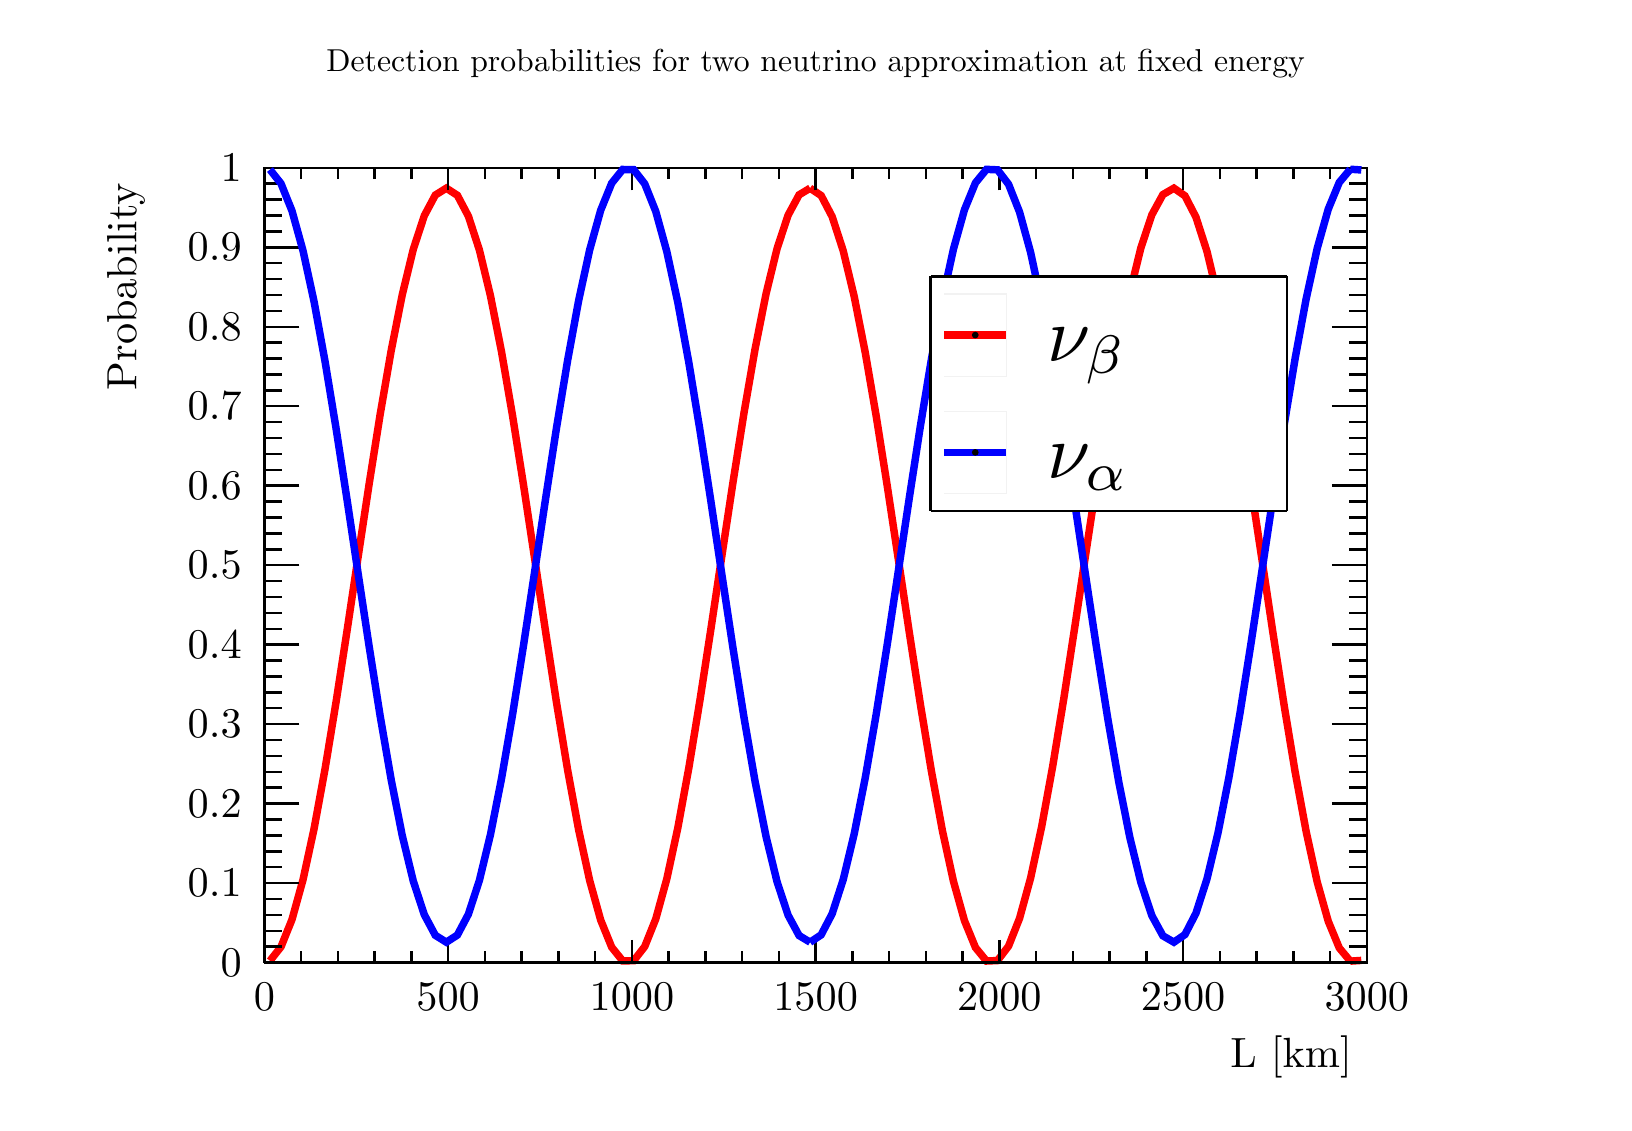
\begin{tikzpicture}
\pgfdeclareplotmark{cross} {
\pgfpathmoveto{\pgfpoint{-0.3\pgfplotmarksize}{\pgfplotmarksize}}
\pgfpathlineto{\pgfpoint{+0.3\pgfplotmarksize}{\pgfplotmarksize}}
\pgfpathlineto{\pgfpoint{+0.3\pgfplotmarksize}{0.3\pgfplotmarksize}}
\pgfpathlineto{\pgfpoint{+1\pgfplotmarksize}{0.3\pgfplotmarksize}}
\pgfpathlineto{\pgfpoint{+1\pgfplotmarksize}{-0.3\pgfplotmarksize}}
\pgfpathlineto{\pgfpoint{+0.3\pgfplotmarksize}{-0.3\pgfplotmarksize}}
\pgfpathlineto{\pgfpoint{+0.3\pgfplotmarksize}{-1.\pgfplotmarksize}}
\pgfpathlineto{\pgfpoint{-0.3\pgfplotmarksize}{-1.\pgfplotmarksize}}
\pgfpathlineto{\pgfpoint{-0.3\pgfplotmarksize}{-0.3\pgfplotmarksize}}
\pgfpathlineto{\pgfpoint{-1.\pgfplotmarksize}{-0.3\pgfplotmarksize}}
\pgfpathlineto{\pgfpoint{-1.\pgfplotmarksize}{0.3\pgfplotmarksize}}
\pgfpathlineto{\pgfpoint{-0.3\pgfplotmarksize}{0.3\pgfplotmarksize}}
\pgfpathclose
\pgfusepathqstroke
}
\pgfdeclareplotmark{cross*} {
\pgfpathmoveto{\pgfpoint{-0.3\pgfplotmarksize}{\pgfplotmarksize}}
\pgfpathlineto{\pgfpoint{+0.3\pgfplotmarksize}{\pgfplotmarksize}}
\pgfpathlineto{\pgfpoint{+0.3\pgfplotmarksize}{0.3\pgfplotmarksize}}
\pgfpathlineto{\pgfpoint{+1\pgfplotmarksize}{0.3\pgfplotmarksize}}
\pgfpathlineto{\pgfpoint{+1\pgfplotmarksize}{-0.3\pgfplotmarksize}}
\pgfpathlineto{\pgfpoint{+0.3\pgfplotmarksize}{-0.3\pgfplotmarksize}}
\pgfpathlineto{\pgfpoint{+0.3\pgfplotmarksize}{-1.\pgfplotmarksize}}
\pgfpathlineto{\pgfpoint{-0.3\pgfplotmarksize}{-1.\pgfplotmarksize}}
\pgfpathlineto{\pgfpoint{-0.3\pgfplotmarksize}{-0.3\pgfplotmarksize}}
\pgfpathlineto{\pgfpoint{-1.\pgfplotmarksize}{-0.3\pgfplotmarksize}}
\pgfpathlineto{\pgfpoint{-1.\pgfplotmarksize}{0.3\pgfplotmarksize}}
\pgfpathlineto{\pgfpoint{-0.3\pgfplotmarksize}{0.3\pgfplotmarksize}}
\pgfpathclose
\pgfusepathqfillstroke
}
\pgfdeclareplotmark{newstar} {
\pgfpathmoveto{\pgfqpoint{0pt}{\pgfplotmarksize}}
\pgfpathlineto{\pgfqpointpolar{44}{0.5\pgfplotmarksize}}
\pgfpathlineto{\pgfqpointpolar{18}{\pgfplotmarksize}}
\pgfpathlineto{\pgfqpointpolar{-20}{0.5\pgfplotmarksize}}
\pgfpathlineto{\pgfqpointpolar{-54}{\pgfplotmarksize}}
\pgfpathlineto{\pgfqpointpolar{-90}{0.5\pgfplotmarksize}}
\pgfpathlineto{\pgfqpointpolar{234}{\pgfplotmarksize}}
\pgfpathlineto{\pgfqpointpolar{198}{0.5\pgfplotmarksize}}
\pgfpathlineto{\pgfqpointpolar{162}{\pgfplotmarksize}}
\pgfpathlineto{\pgfqpointpolar{134}{0.5\pgfplotmarksize}}
\pgfpathclose
\pgfusepathqstroke
}
\pgfdeclareplotmark{newstar*} {
\pgfpathmoveto{\pgfqpoint{0pt}{\pgfplotmarksize}}
\pgfpathlineto{\pgfqpointpolar{44}{0.5\pgfplotmarksize}}
\pgfpathlineto{\pgfqpointpolar{18}{\pgfplotmarksize}}
\pgfpathlineto{\pgfqpointpolar{-20}{0.5\pgfplotmarksize}}
\pgfpathlineto{\pgfqpointpolar{-54}{\pgfplotmarksize}}
\pgfpathlineto{\pgfqpointpolar{-90}{0.5\pgfplotmarksize}}
\pgfpathlineto{\pgfqpointpolar{234}{\pgfplotmarksize}}
\pgfpathlineto{\pgfqpointpolar{198}{0.5\pgfplotmarksize}}
\pgfpathlineto{\pgfqpointpolar{162}{\pgfplotmarksize}}
\pgfpathlineto{\pgfqpointpolar{134}{0.5\pgfplotmarksize}}
\pgfpathclose
\pgfusepathqfillstroke
}
\definecolor{c}{rgb}{1,1,1};
\draw [color=c, fill=c] (0,0) rectangle (20,13.639);
\draw [color=c, fill=c] (3,1.77307) rectangle (17,11.8659);
\definecolor{c}{rgb}{0,0,0};
\draw [c,line width=0.9] (3,1.77307) -- (3,11.8659) -- (17,11.8659) -- (17,1.77307) -- (3,1.77307);
\definecolor{c}{rgb}{1,1,1};
\draw [color=c, fill=c] (3,1.77307) rectangle (17,11.8659);
\definecolor{c}{rgb}{0,0,0};
\draw [c,line width=0.9] (3,1.77307) -- (3,11.8659) -- (17,11.8659) -- (17,1.77307) -- (3,1.77307);
\definecolor{c}{rgb}{1,0,0};
\draw [c,line width=2.7] (3.07,1.79535) -- (3.21,1.97246) -- (3.35,2.32025) -- (3.49,2.82616) -- (3.63,3.47188) -- (3.77,4.23404) -- (3.91,5.08507) -- (4.05,5.99418) -- (4.19,6.92847) -- (4.33,7.85415) -- (4.47,8.73772) -- (4.61,9.54721) --
 (4.75,10.2533) -- (4.89,10.8306) -- (5.03,11.258) -- (5.17,11.5201) -- (5.31,11.6075) -- (5.45,11.517) -- (5.59,11.2519) -- (5.73,10.8217) -- (5.87,10.2421) -- (6.01,9.53393) -- (6.15,8.72289) -- (6.29,7.83831) -- (6.43,6.91219) -- (6.57,5.97805) --
 (6.71,5.06967) -- (6.85,4.21993) -- (6.99,3.45957) -- (7.13,2.8161) -- (7.27,2.31281) -- (7.41,1.96789) -- (7.55,1.79383) -- (7.69,1.79693) -- (7.83,1.97708) -- (7.97,2.32775) -- (8.11,2.83626) -- (8.25,3.48422) -- (8.39,4.24817) -- (8.53,5.10048)
 -- (8.67,6.01032) -- (8.81,6.94475) -- (8.95,7.86998) -- (9.09,8.75253) -- (9.23,9.56046) -- (9.37,10.2646) -- (9.51,10.8393) -- (9.65,11.264) -- (9.79,11.5232) -- (9.93,11.6075);
\draw [c,line width=2.7] (9.93,11.6075) -- (10.07,11.5139) -- (10.21,11.2458) -- (10.35,10.8129) -- (10.49,10.2308) -- (10.63,9.52062) -- (10.77,8.70804) -- (10.91,7.82245) -- (11.05,6.89591) -- (11.19,5.96192) -- (11.33,5.05429) -- (11.47,4.20585)
 -- (11.61,3.4473) -- (11.75,2.80609) -- (11.89,2.30541) -- (12.03,1.96337) -- (12.17,1.79236) -- (12.31,1.79856) -- (12.45,1.98175) -- (12.59,2.3353) -- (12.73,2.84641) -- (12.87,3.4966) -- (13.01,4.26233) -- (13.15,5.11592) -- (13.29,6.02646) --
 (13.43,6.96103) -- (13.57,7.8858) -- (13.71,8.76731) -- (13.85,9.57368) -- (13.99,10.2757) -- (14.13,10.8481) -- (14.27,11.2699) -- (14.41,11.5261) -- (14.55,11.6074) -- (14.69,11.5107) -- (14.83,11.2396) -- (14.97,10.804) -- (15.11,10.2195) --
 (15.25,9.50727) -- (15.39,8.69316) -- (15.53,7.80659) -- (15.67,6.87962) -- (15.81,5.94581) -- (15.95,5.03893) -- (16.09,4.1918) -- (16.23,3.43507) -- (16.37,2.79611) -- (16.51,2.29805) -- (16.65,1.95891) -- (16.79,1.79095);
\draw [c,line width=2.7] (16.79,1.79095) -- (16.93,1.80025);
\definecolor{c}{rgb}{0,0,0};
\draw [c,line width=0.9] (3,1.77307) -- (17,1.77307);
\draw [c,line width=0.9] (3,2.05948) -- (3,1.77307);
\draw [c,line width=0.9] (3.46667,1.91628) -- (3.46667,1.77307);
\draw [c,line width=0.9] (3.93333,1.91628) -- (3.93333,1.77307);
\draw [c,line width=0.9] (4.4,1.91628) -- (4.4,1.77307);
\draw [c,line width=0.9] (4.86667,1.91628) -- (4.86667,1.77307);
\draw [c,line width=0.9] (5.33333,2.05948) -- (5.33333,1.77307);
\draw [c,line width=0.9] (5.8,1.91628) -- (5.8,1.77307);
\draw [c,line width=0.9] (6.26667,1.91628) -- (6.26667,1.77307);
\draw [c,line width=0.9] (6.73333,1.91628) -- (6.73333,1.77307);
\draw [c,line width=0.9] (7.2,1.91628) -- (7.2,1.77307);
\draw [c,line width=0.9] (7.66667,2.05948) -- (7.66667,1.77307);
\draw [c,line width=0.9] (8.13333,1.91628) -- (8.13333,1.77307);
\draw [c,line width=0.9] (8.6,1.91628) -- (8.6,1.77307);
\draw [c,line width=0.9] (9.06667,1.91628) -- (9.06667,1.77307);
\draw [c,line width=0.9] (9.53333,1.91628) -- (9.53333,1.77307);
\draw [c,line width=0.9] (10,2.05948) -- (10,1.77307);
\draw [c,line width=0.9] (10.4667,1.91628) -- (10.4667,1.77307);
\draw [c,line width=0.9] (10.9333,1.91628) -- (10.9333,1.77307);
\draw [c,line width=0.9] (11.4,1.91628) -- (11.4,1.77307);
\draw [c,line width=0.9] (11.8667,1.91628) -- (11.8667,1.77307);
\draw [c,line width=0.9] (12.3333,2.05948) -- (12.3333,1.77307);
\draw [c,line width=0.9] (12.8,1.91628) -- (12.8,1.77307);
\draw [c,line width=0.9] (13.2667,1.91628) -- (13.2667,1.77307);
\draw [c,line width=0.9] (13.7333,1.91628) -- (13.7333,1.77307);
\draw [c,line width=0.9] (14.2,1.91628) -- (14.2,1.77307);
\draw [c,line width=0.9] (14.6667,2.05948) -- (14.6667,1.77307);
\draw [c,line width=0.9] (15.1333,1.91628) -- (15.1333,1.77307);
\draw [c,line width=0.9] (15.6,1.91628) -- (15.6,1.77307);
\draw [c,line width=0.9] (16.0667,1.91628) -- (16.0667,1.77307);
\draw [c,line width=0.9] (16.5333,1.91628) -- (16.5333,1.77307);
\draw [c,line width=0.9] (17,2.05948) -- (17,1.77307);
\draw [anchor=base] (3,1.15931) node[scale=1.52731, color=c, rotate=0]{0};
\draw [anchor=base] (5.33333,1.15931) node[scale=1.52731, color=c, rotate=0]{500};
\draw [anchor=base] (7.66667,1.15931) node[scale=1.52731, color=c, rotate=0]{1000};
\draw [anchor=base] (10,1.15931) node[scale=1.52731, color=c, rotate=0]{1500};
\draw [anchor=base] (12.3333,1.15931) node[scale=1.52731, color=c, rotate=0]{2000};
\draw [anchor=base] (14.6667,1.15931) node[scale=1.52731, color=c, rotate=0]{2500};
\draw [anchor=base] (17,1.15931) node[scale=1.52731, color=c, rotate=0]{3000};
\draw [anchor= east] (17,0.572837) node[scale=1.52731, color=c, rotate=0]{L [km]};
\draw [c,line width=0.9] (3,11.8659) -- (17,11.8659);
\draw [c,line width=0.9] (3,11.5795) -- (3,11.8659);
\draw [c,line width=0.9] (3.46667,11.7227) -- (3.46667,11.8659);
\draw [c,line width=0.9] (3.93333,11.7227) -- (3.93333,11.8659);
\draw [c,line width=0.9] (4.4,11.7227) -- (4.4,11.8659);
\draw [c,line width=0.9] (4.86667,11.7227) -- (4.86667,11.8659);
\draw [c,line width=0.9] (5.33333,11.5795) -- (5.33333,11.8659);
\draw [c,line width=0.9] (5.8,11.7227) -- (5.8,11.8659);
\draw [c,line width=0.9] (6.26667,11.7227) -- (6.26667,11.8659);
\draw [c,line width=0.9] (6.73333,11.7227) -- (6.73333,11.8659);
\draw [c,line width=0.9] (7.2,11.7227) -- (7.2,11.8659);
\draw [c,line width=0.9] (7.66667,11.5795) -- (7.66667,11.8659);
\draw [c,line width=0.9] (8.13333,11.7227) -- (8.13333,11.8659);
\draw [c,line width=0.9] (8.6,11.7227) -- (8.6,11.8659);
\draw [c,line width=0.9] (9.06667,11.7227) -- (9.06667,11.8659);
\draw [c,line width=0.9] (9.53333,11.7227) -- (9.53333,11.8659);
\draw [c,line width=0.9] (10,11.5795) -- (10,11.8659);
\draw [c,line width=0.9] (10.4667,11.7227) -- (10.4667,11.8659);
\draw [c,line width=0.9] (10.9333,11.7227) -- (10.9333,11.8659);
\draw [c,line width=0.9] (11.4,11.7227) -- (11.4,11.8659);
\draw [c,line width=0.9] (11.8667,11.7227) -- (11.8667,11.8659);
\draw [c,line width=0.9] (12.3333,11.5795) -- (12.3333,11.8659);
\draw [c,line width=0.9] (12.8,11.7227) -- (12.8,11.8659);
\draw [c,line width=0.9] (13.2667,11.7227) -- (13.2667,11.8659);
\draw [c,line width=0.9] (13.7333,11.7227) -- (13.7333,11.8659);
\draw [c,line width=0.9] (14.2,11.7227) -- (14.2,11.8659);
\draw [c,line width=0.9] (14.6667,11.5795) -- (14.6667,11.8659);
\draw [c,line width=0.9] (15.1333,11.7227) -- (15.1333,11.8659);
\draw [c,line width=0.9] (15.6,11.7227) -- (15.6,11.8659);
\draw [c,line width=0.9] (16.0667,11.7227) -- (16.0667,11.8659);
\draw [c,line width=0.9] (16.5333,11.7227) -- (16.5333,11.8659);
\draw [c,line width=0.9] (17,11.5795) -- (17,11.8659);
\draw [c,line width=0.9] (3,1.77307) -- (3,11.8659);
\draw [c,line width=0.9] (3.444,1.77307) -- (3,1.77307);
\draw [c,line width=0.9] (3.222,1.97492) -- (3,1.97492);
\draw [c,line width=0.9] (3.222,2.17678) -- (3,2.17678);
\draw [c,line width=0.9] (3.222,2.37864) -- (3,2.37864);
\draw [c,line width=0.9] (3.222,2.58049) -- (3,2.58049);
\draw [c,line width=0.9] (3.444,2.78235) -- (3,2.78235);
\draw [c,line width=0.9] (3.222,2.98421) -- (3,2.98421);
\draw [c,line width=0.9] (3.222,3.18606) -- (3,3.18606);
\draw [c,line width=0.9] (3.222,3.38792) -- (3,3.38792);
\draw [c,line width=0.9] (3.222,3.58978) -- (3,3.58978);
\draw [c,line width=0.9] (3.444,3.79163) -- (3,3.79163);
\draw [c,line width=0.9] (3.222,3.99349) -- (3,3.99349);
\draw [c,line width=0.9] (3.222,4.19535) -- (3,4.19535);
\draw [c,line width=0.9] (3.222,4.3972) -- (3,4.3972);
\draw [c,line width=0.9] (3.222,4.59906) -- (3,4.59906);
\draw [c,line width=0.9] (3.444,4.80092) -- (3,4.80092);
\draw [c,line width=0.9] (3.222,5.00277) -- (3,5.00277);
\draw [c,line width=0.9] (3.222,5.20463) -- (3,5.20463);
\draw [c,line width=0.9] (3.222,5.40649) -- (3,5.40649);
\draw [c,line width=0.9] (3.222,5.60834) -- (3,5.60834);
\draw [c,line width=0.9] (3.444,5.8102) -- (3,5.8102);
\draw [c,line width=0.9] (3.222,6.01206) -- (3,6.01206);
\draw [c,line width=0.9] (3.222,6.21391) -- (3,6.21391);
\draw [c,line width=0.9] (3.222,6.41577) -- (3,6.41577);
\draw [c,line width=0.9] (3.222,6.61763) -- (3,6.61763);
\draw [c,line width=0.9] (3.444,6.81948) -- (3,6.81948);
\draw [c,line width=0.9] (3.222,7.02134) -- (3,7.02134);
\draw [c,line width=0.9] (3.222,7.2232) -- (3,7.2232);
\draw [c,line width=0.9] (3.222,7.42505) -- (3,7.42505);
\draw [c,line width=0.9] (3.222,7.62691) -- (3,7.62691);
\draw [c,line width=0.9] (3.444,7.82877) -- (3,7.82877);
\draw [c,line width=0.9] (3.222,8.03062) -- (3,8.03062);
\draw [c,line width=0.9] (3.222,8.23248) -- (3,8.23248);
\draw [c,line width=0.9] (3.222,8.43434) -- (3,8.43434);
\draw [c,line width=0.9] (3.222,8.6362) -- (3,8.6362);
\draw [c,line width=0.9] (3.444,8.83805) -- (3,8.83805);
\draw [c,line width=0.9] (3.222,9.03991) -- (3,9.03991);
\draw [c,line width=0.9] (3.222,9.24177) -- (3,9.24177);
\draw [c,line width=0.9] (3.222,9.44362) -- (3,9.44362);
\draw [c,line width=0.9] (3.222,9.64548) -- (3,9.64548);
\draw [c,line width=0.9] (3.444,9.84733) -- (3,9.84733);
\draw [c,line width=0.9] (3.222,10.0492) -- (3,10.0492);
\draw [c,line width=0.9] (3.222,10.251) -- (3,10.251);
\draw [c,line width=0.9] (3.222,10.4529) -- (3,10.4529);
\draw [c,line width=0.9] (3.222,10.6548) -- (3,10.6548);
\draw [c,line width=0.9] (3.444,10.8566) -- (3,10.8566);
\draw [c,line width=0.9] (3.222,11.0585) -- (3,11.0585);
\draw [c,line width=0.9] (3.222,11.2603) -- (3,11.2603);
\draw [c,line width=0.9] (3.222,11.4622) -- (3,11.4622);
\draw [c,line width=0.9] (3.222,11.664) -- (3,11.664);
\draw [c,line width=0.9] (3.444,11.8659) -- (3,11.8659);
\draw [anchor= east] (2.9,1.77307) node[scale=1.52731, color=c, rotate=0]{0};
\draw [anchor= east] (2.9,2.78235) node[scale=1.52731, color=c, rotate=0]{0.1};
\draw [anchor= east] (2.9,3.79163) node[scale=1.52731, color=c, rotate=0]{0.2};
\draw [anchor= east] (2.9,4.80092) node[scale=1.52731, color=c, rotate=0]{0.3};
\draw [anchor= east] (2.9,5.8102) node[scale=1.52731, color=c, rotate=0]{0.4};
\draw [anchor= east] (2.9,6.81948) node[scale=1.52731, color=c, rotate=0]{0.5};
\draw [anchor= east] (2.9,7.82877) node[scale=1.52731, color=c, rotate=0]{0.6};
\draw [anchor= east] (2.9,8.83805) node[scale=1.52731, color=c, rotate=0]{0.7};
\draw [anchor= east] (2.9,9.84733) node[scale=1.52731, color=c, rotate=0]{0.8};
\draw [anchor= east] (2.9,10.8566) node[scale=1.52731, color=c, rotate=0]{0.9};
\draw [anchor= east] (2.9,11.8659) node[scale=1.52731, color=c, rotate=0]{1};
\draw [anchor= east] (1.24,11.8659) node[scale=1.52731, color=c, rotate=90]{Probability};
\draw [c,line width=0.9] (17,1.77307) -- (17,11.8659);
\draw [c,line width=0.9] (16.556,1.77307) -- (17,1.77307);
\draw [c,line width=0.9] (16.778,1.97492) -- (17,1.97492);
\draw [c,line width=0.9] (16.778,2.17678) -- (17,2.17678);
\draw [c,line width=0.9] (16.778,2.37864) -- (17,2.37864);
\draw [c,line width=0.9] (16.778,2.58049) -- (17,2.58049);
\draw [c,line width=0.9] (16.556,2.78235) -- (17,2.78235);
\draw [c,line width=0.9] (16.778,2.98421) -- (17,2.98421);
\draw [c,line width=0.9] (16.778,3.18606) -- (17,3.18606);
\draw [c,line width=0.9] (16.778,3.38792) -- (17,3.38792);
\draw [c,line width=0.9] (16.778,3.58978) -- (17,3.58978);
\draw [c,line width=0.9] (16.556,3.79163) -- (17,3.79163);
\draw [c,line width=0.9] (16.778,3.99349) -- (17,3.99349);
\draw [c,line width=0.9] (16.778,4.19535) -- (17,4.19535);
\draw [c,line width=0.9] (16.778,4.3972) -- (17,4.3972);
\draw [c,line width=0.9] (16.778,4.59906) -- (17,4.59906);
\draw [c,line width=0.9] (16.556,4.80092) -- (17,4.80092);
\draw [c,line width=0.9] (16.778,5.00277) -- (17,5.00277);
\draw [c,line width=0.9] (16.778,5.20463) -- (17,5.20463);
\draw [c,line width=0.9] (16.778,5.40649) -- (17,5.40649);
\draw [c,line width=0.9] (16.778,5.60834) -- (17,5.60834);
\draw [c,line width=0.9] (16.556,5.8102) -- (17,5.8102);
\draw [c,line width=0.9] (16.778,6.01206) -- (17,6.01206);
\draw [c,line width=0.9] (16.778,6.21391) -- (17,6.21391);
\draw [c,line width=0.9] (16.778,6.41577) -- (17,6.41577);
\draw [c,line width=0.9] (16.778,6.61763) -- (17,6.61763);
\draw [c,line width=0.9] (16.556,6.81948) -- (17,6.81948);
\draw [c,line width=0.9] (16.778,7.02134) -- (17,7.02134);
\draw [c,line width=0.9] (16.778,7.2232) -- (17,7.2232);
\draw [c,line width=0.9] (16.778,7.42505) -- (17,7.42505);
\draw [c,line width=0.9] (16.778,7.62691) -- (17,7.62691);
\draw [c,line width=0.9] (16.556,7.82877) -- (17,7.82877);
\draw [c,line width=0.9] (16.778,8.03062) -- (17,8.03062);
\draw [c,line width=0.9] (16.778,8.23248) -- (17,8.23248);
\draw [c,line width=0.9] (16.778,8.43434) -- (17,8.43434);
\draw [c,line width=0.9] (16.778,8.6362) -- (17,8.6362);
\draw [c,line width=0.9] (16.556,8.83805) -- (17,8.83805);
\draw [c,line width=0.9] (16.778,9.03991) -- (17,9.03991);
\draw [c,line width=0.9] (16.778,9.24177) -- (17,9.24177);
\draw [c,line width=0.9] (16.778,9.44362) -- (17,9.44362);
\draw [c,line width=0.9] (16.778,9.64548) -- (17,9.64548);
\draw [c,line width=0.9] (16.556,9.84733) -- (17,9.84733);
\draw [c,line width=0.9] (16.778,10.0492) -- (17,10.0492);
\draw [c,line width=0.9] (16.778,10.251) -- (17,10.251);
\draw [c,line width=0.9] (16.778,10.4529) -- (17,10.4529);
\draw [c,line width=0.9] (16.778,10.6548) -- (17,10.6548);
\draw [c,line width=0.9] (16.556,10.8566) -- (17,10.8566);
\draw [c,line width=0.9] (16.778,11.0585) -- (17,11.0585);
\draw [c,line width=0.9] (16.778,11.2603) -- (17,11.2603);
\draw [c,line width=0.9] (16.778,11.4622) -- (17,11.4622);
\draw [c,line width=0.9] (16.778,11.664) -- (17,11.664);
\draw [c,line width=0.9] (16.556,11.8659) -- (17,11.8659);
\definecolor{c}{rgb}{0,0,1};
\draw [c,line width=2.7] (3.07,11.8436) -- (3.21,11.6665) -- (3.35,11.3187) -- (3.49,10.8128) -- (3.63,10.1671) -- (3.77,9.40493) -- (3.91,8.5539) -- (4.05,7.64479) -- (4.19,6.7105) -- (4.33,5.78482) -- (4.47,4.90125) -- (4.61,4.09176) --
 (4.75,3.38563) -- (4.89,2.80841) -- (5.03,2.381) -- (5.17,2.11884) -- (5.31,2.03143) -- (5.45,2.12192) -- (5.59,2.38706) -- (5.73,2.81723) -- (5.87,3.39688) -- (6.01,4.10504) -- (6.15,4.91608) -- (6.29,5.80066) -- (6.43,6.72678) -- (6.57,7.66092) --
 (6.71,8.5693) -- (6.85,9.41904) -- (6.99,10.1794) -- (7.13,10.8229) -- (7.27,11.3262) -- (7.41,11.6711) -- (7.55,11.8451) -- (7.69,11.842) -- (7.83,11.6619) -- (7.97,11.3112) -- (8.11,10.8027) -- (8.25,10.1547) -- (8.39,9.3908) -- (8.53,8.53848) --
 (8.67,7.62865) -- (8.81,6.69422) -- (8.95,5.76899) -- (9.09,4.88644) -- (9.23,4.07851) -- (9.37,3.37442) -- (9.51,2.79964) -- (9.65,2.37498) -- (9.79,2.1158) -- (9.93,2.03148);
\draw [c,line width=2.7] (9.93,2.03148) -- (10.07,2.12506) -- (10.21,2.39317) -- (10.35,2.82609) -- (10.49,3.40817) -- (10.63,4.11835) -- (10.77,4.93093) -- (10.91,5.81652) -- (11.05,6.74306) -- (11.19,7.67705) -- (11.33,8.58468) -- (11.47,9.43312)
 -- (11.61,10.1917) -- (11.75,10.8329) -- (11.89,11.3336) -- (12.03,11.6756) -- (12.17,11.8466) -- (12.31,11.8404) -- (12.45,11.6572) -- (12.59,11.3037) -- (12.73,10.7926) -- (12.87,10.1424) -- (13.01,9.37664) -- (13.15,8.52305) -- (13.29,7.61251) --
 (13.43,6.67794) -- (13.57,5.75317) -- (13.71,4.87166) -- (13.85,4.06529) -- (13.99,3.36324) -- (14.13,2.79092) -- (14.27,2.36902) -- (14.41,2.11282) -- (14.55,2.03159) -- (14.69,2.12826) -- (14.83,2.39933) -- (14.97,2.835) -- (15.11,3.4195) --
 (15.25,4.1317) -- (15.39,4.94581) -- (15.53,5.83238) -- (15.67,6.75935) -- (15.81,7.69316) -- (15.95,8.60004) -- (16.09,9.44717) -- (16.23,10.2039) -- (16.37,10.8429) -- (16.51,11.3409) -- (16.65,11.6801) -- (16.79,11.848);
\draw [c,line width=2.7] (16.79,11.848) -- (16.93,11.8387);
\definecolor{c}{rgb}{1,1,1};
\draw [color=c, fill=c] (2,12.8206) rectangle (18,13.5708);
\definecolor{c}{rgb}{0,0,0};
\draw (10,13.1957) node[scale=1.14549, color=c, rotate=0]{Detection probabilities for two neutrino approximation at fixed energy};
\definecolor{c}{rgb}{1,1,1};
\draw [color=c, fill=c] (11.4613,7.50716) rectangle (15.9885,10.4871);
\definecolor{c}{rgb}{0,0,0};
\draw [c,line width=0.9] (11.4613,7.50716) -- (15.9885,7.50716);
\draw [c,line width=0.9] (15.9885,7.50716) -- (15.9885,10.4871);
\draw [c,line width=0.9] (15.9885,10.4871) -- (11.4613,10.4871);
\draw [c,line width=0.9] (11.4613,10.4871) -- (11.4613,7.50716);
\draw [anchor=base west] (12.5931,9.40688) node[scale=2.80008, color=c, rotate=0]{$\nu_{\beta}$};
\definecolor{c}{rgb}{0.95,0.95,0.95};
\draw [c] (11.6311,9.22063) -- (12.4234,9.22063) -- (12.4234,10.2636) -- (11.6311,10.2636);
\definecolor{c}{rgb}{1,0,0};
\draw [c,line width=2.7] (11.6311,9.74212) -- (12.4234,9.74212);
\definecolor{c}{rgb}{0,0,0};
\foreach \P in {(12.0272,9.74212)}{\draw[mark options={color=c,fill=c},mark size=2.402402pt,mark=*,mark size=1pt] plot coordinates {\P};}
\draw [anchor=base west] (12.5931,7.91691) node[scale=2.80008, color=c, rotate=0]{$\nu_{\alpha}$};
\definecolor{c}{rgb}{0.95,0.95,0.95};
\draw [c] (11.6311,7.73066) -- (12.4234,7.73066) -- (12.4234,8.77364) -- (11.6311,8.77364);
\definecolor{c}{rgb}{0,0,1};
\draw [c,line width=2.7] (11.6311,8.25215) -- (12.4234,8.25215);
\definecolor{c}{rgb}{0,0,0};
\foreach \P in {(12.0272,8.25215)}{\draw[mark options={color=c,fill=c},mark size=2.402402pt,mark=*,mark size=1pt] plot coordinates {\P};}
\end{tikzpicture}

    \end{adjustbox}
    \caption{Probability of detecting an initial $\nu_{\alpha}$ as a particular flavour as a function of baseline, $L$. Here, the energy of the neutrino is 1~GeV.}
  \end{subfigure}
  \hfill
  \begin{subfigure}[t]{0.49\textwidth}
    \begin{adjustbox}{max totalsize={\textwidth}, center}
      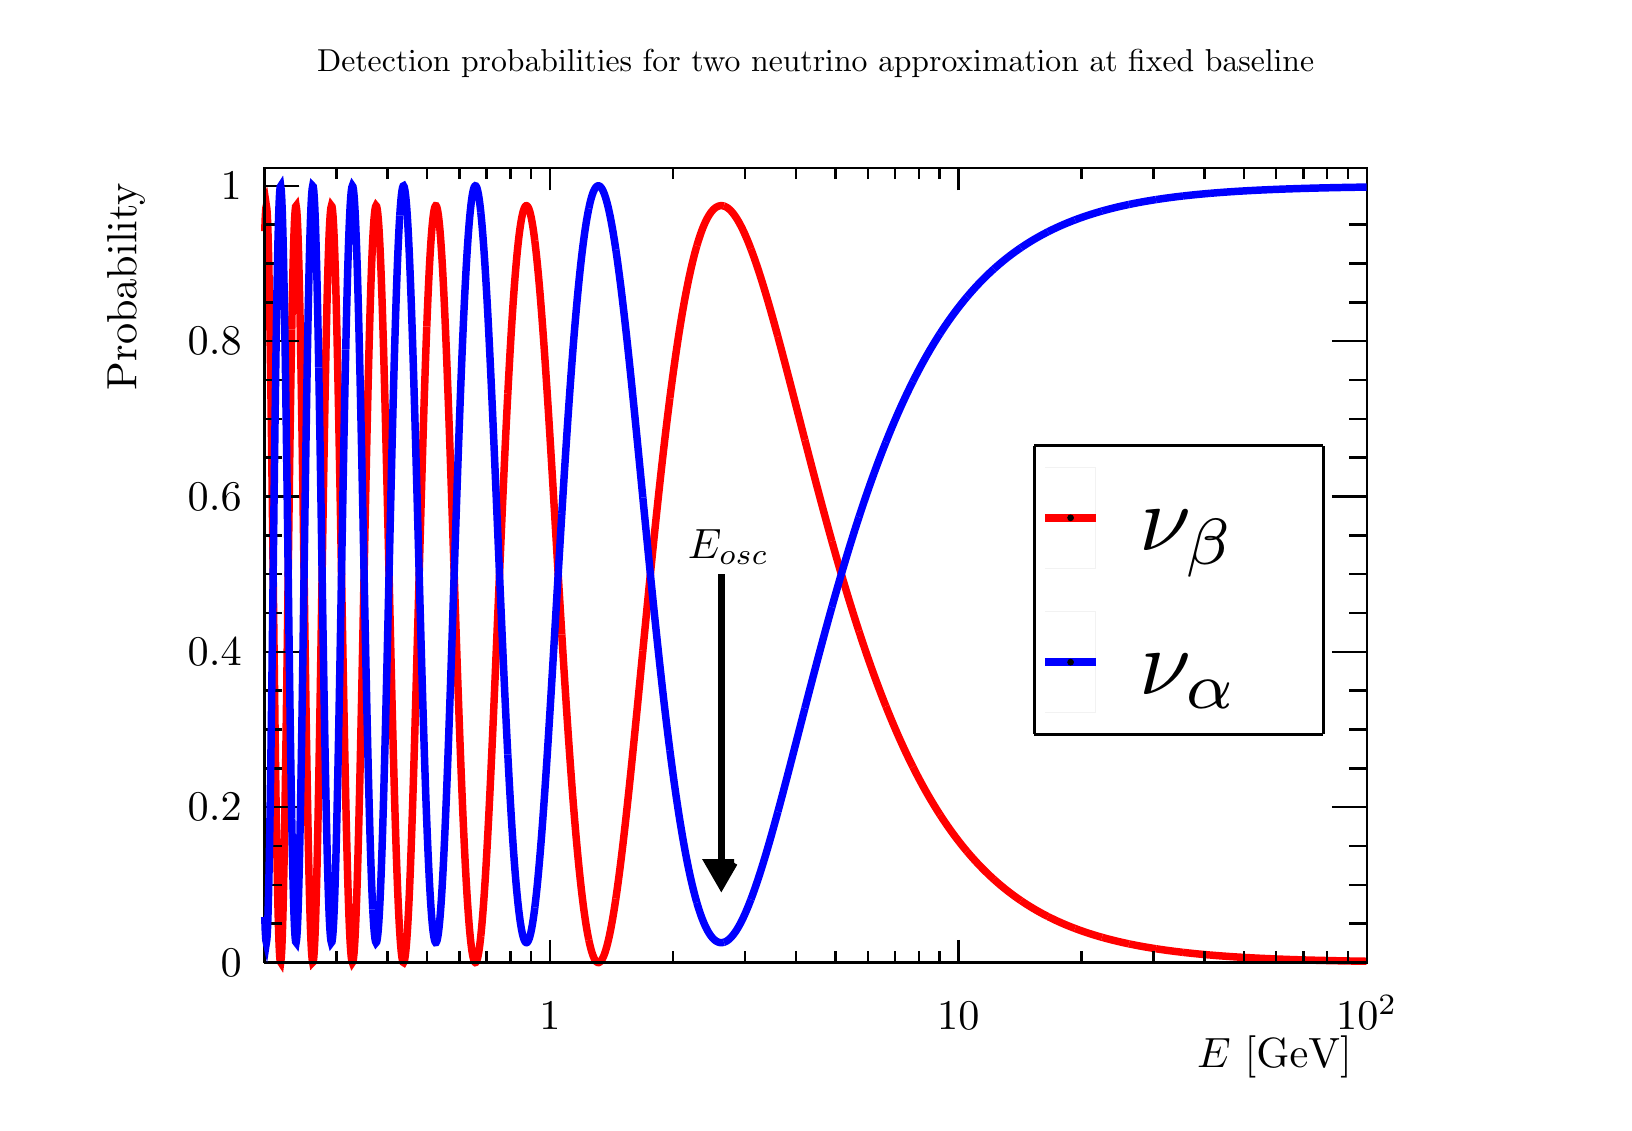
\begin{tikzpicture}
\pgfdeclareplotmark{cross} {
\pgfpathmoveto{\pgfpoint{-0.3\pgfplotmarksize}{\pgfplotmarksize}}
\pgfpathlineto{\pgfpoint{+0.3\pgfplotmarksize}{\pgfplotmarksize}}
\pgfpathlineto{\pgfpoint{+0.3\pgfplotmarksize}{0.3\pgfplotmarksize}}
\pgfpathlineto{\pgfpoint{+1\pgfplotmarksize}{0.3\pgfplotmarksize}}
\pgfpathlineto{\pgfpoint{+1\pgfplotmarksize}{-0.3\pgfplotmarksize}}
\pgfpathlineto{\pgfpoint{+0.3\pgfplotmarksize}{-0.3\pgfplotmarksize}}
\pgfpathlineto{\pgfpoint{+0.3\pgfplotmarksize}{-1.\pgfplotmarksize}}
\pgfpathlineto{\pgfpoint{-0.3\pgfplotmarksize}{-1.\pgfplotmarksize}}
\pgfpathlineto{\pgfpoint{-0.3\pgfplotmarksize}{-0.3\pgfplotmarksize}}
\pgfpathlineto{\pgfpoint{-1.\pgfplotmarksize}{-0.3\pgfplotmarksize}}
\pgfpathlineto{\pgfpoint{-1.\pgfplotmarksize}{0.3\pgfplotmarksize}}
\pgfpathlineto{\pgfpoint{-0.3\pgfplotmarksize}{0.3\pgfplotmarksize}}
\pgfpathclose
\pgfusepathqstroke
}
\pgfdeclareplotmark{cross*} {
\pgfpathmoveto{\pgfpoint{-0.3\pgfplotmarksize}{\pgfplotmarksize}}
\pgfpathlineto{\pgfpoint{+0.3\pgfplotmarksize}{\pgfplotmarksize}}
\pgfpathlineto{\pgfpoint{+0.3\pgfplotmarksize}{0.3\pgfplotmarksize}}
\pgfpathlineto{\pgfpoint{+1\pgfplotmarksize}{0.3\pgfplotmarksize}}
\pgfpathlineto{\pgfpoint{+1\pgfplotmarksize}{-0.3\pgfplotmarksize}}
\pgfpathlineto{\pgfpoint{+0.3\pgfplotmarksize}{-0.3\pgfplotmarksize}}
\pgfpathlineto{\pgfpoint{+0.3\pgfplotmarksize}{-1.\pgfplotmarksize}}
\pgfpathlineto{\pgfpoint{-0.3\pgfplotmarksize}{-1.\pgfplotmarksize}}
\pgfpathlineto{\pgfpoint{-0.3\pgfplotmarksize}{-0.3\pgfplotmarksize}}
\pgfpathlineto{\pgfpoint{-1.\pgfplotmarksize}{-0.3\pgfplotmarksize}}
\pgfpathlineto{\pgfpoint{-1.\pgfplotmarksize}{0.3\pgfplotmarksize}}
\pgfpathlineto{\pgfpoint{-0.3\pgfplotmarksize}{0.3\pgfplotmarksize}}
\pgfpathclose
\pgfusepathqfillstroke
}
\pgfdeclareplotmark{newstar} {
\pgfpathmoveto{\pgfqpoint{0pt}{\pgfplotmarksize}}
\pgfpathlineto{\pgfqpointpolar{44}{0.5\pgfplotmarksize}}
\pgfpathlineto{\pgfqpointpolar{18}{\pgfplotmarksize}}
\pgfpathlineto{\pgfqpointpolar{-20}{0.5\pgfplotmarksize}}
\pgfpathlineto{\pgfqpointpolar{-54}{\pgfplotmarksize}}
\pgfpathlineto{\pgfqpointpolar{-90}{0.5\pgfplotmarksize}}
\pgfpathlineto{\pgfqpointpolar{234}{\pgfplotmarksize}}
\pgfpathlineto{\pgfqpointpolar{198}{0.5\pgfplotmarksize}}
\pgfpathlineto{\pgfqpointpolar{162}{\pgfplotmarksize}}
\pgfpathlineto{\pgfqpointpolar{134}{0.5\pgfplotmarksize}}
\pgfpathclose
\pgfusepathqstroke
}
\pgfdeclareplotmark{newstar*} {
\pgfpathmoveto{\pgfqpoint{0pt}{\pgfplotmarksize}}
\pgfpathlineto{\pgfqpointpolar{44}{0.5\pgfplotmarksize}}
\pgfpathlineto{\pgfqpointpolar{18}{\pgfplotmarksize}}
\pgfpathlineto{\pgfqpointpolar{-20}{0.5\pgfplotmarksize}}
\pgfpathlineto{\pgfqpointpolar{-54}{\pgfplotmarksize}}
\pgfpathlineto{\pgfqpointpolar{-90}{0.5\pgfplotmarksize}}
\pgfpathlineto{\pgfqpointpolar{234}{\pgfplotmarksize}}
\pgfpathlineto{\pgfqpointpolar{198}{0.5\pgfplotmarksize}}
\pgfpathlineto{\pgfqpointpolar{162}{\pgfplotmarksize}}
\pgfpathlineto{\pgfqpointpolar{134}{0.5\pgfplotmarksize}}
\pgfpathclose
\pgfusepathqfillstroke
}
\definecolor{c}{rgb}{1,1,1};
\draw [color=c, fill=c] (0,0) rectangle (20,13.639);
\draw [color=c, fill=c] (3,1.77307) rectangle (17,11.8659);
\definecolor{c}{rgb}{0,0,0};
\draw [c,line width=0.9] (3,1.77307) -- (3,11.8659) -- (17,11.8659) -- (17,1.77307) -- (3,1.77307);
\definecolor{c}{rgb}{1,1,1};
\draw [color=c, fill=c] (3,1.77307) rectangle (17,11.8659);
\definecolor{c}{rgb}{0,0,0};
\draw [c,line width=0.9] (3,1.77307) -- (3,11.8659) -- (17,11.8659) -- (17,1.77307) -- (3,1.77307);
\definecolor{c}{rgb}{1,0,0};
\draw [c,line width=2.7] (3.0035,11.0598) -- (3.0105,11.2449) -- (3.0175,11.3537) -- (3.0245,11.385) -- (3.0315,11.339) -- (3.0385,11.2174) -- (3.0455,11.0225) -- (3.0525,10.7583) -- (3.0595,10.4295) -- (3.0665,10.0417) -- (3.0735,9.60166) --
 (3.0805,9.1165) -- (3.0875,8.5941) -- (3.0945,8.04273) -- (3.1015,7.47098) -- (3.1085,6.88764) -- (3.1155,6.30149) -- (3.1225,5.72127) -- (3.1295,5.15547) -- (3.1365,4.61223) -- (3.1435,4.09924) -- (3.1505,3.62366) -- (3.1575,3.19196) --
 (3.1645,2.80992) -- (3.1715,2.48248) -- (3.1785,2.21376) -- (3.1855,2.00699) -- (3.1925,1.86448) -- (3.1995,1.7876) -- (3.2065,1.7768) -- (3.2135,1.83162) -- (3.2205,1.95071) -- (3.2275,2.13186) -- (3.2345,2.37207) -- (3.2415,2.66759) --
 (3.2485,3.01398) -- (3.2555,3.40621) -- (3.2625,3.83872) -- (3.2695,4.30551) -- (3.2765,4.80022) -- (3.2835,5.31623) -- (3.2905,5.84676) -- (3.2975,6.38493) -- (3.3045,6.9239) -- (3.3115,7.45687) -- (3.3185,7.97729) -- (3.3255,8.4788) --
 (3.3325,8.95542) -- (3.3395,9.40155) -- (3.3465,9.81205);
\draw [c,line width=2.7] (3.3465,9.81205) -- (3.3535,10.1823) -- (3.3605,10.5082) -- (3.3675,10.7862) -- (3.3745,11.0136) -- (3.3815,11.1882) -- (3.3885,11.3083) -- (3.3955,11.373) -- (3.4025,11.3822) -- (3.4095,11.3363) -- (3.4165,11.2362) --
 (3.4235,11.0836) -- (3.4305,10.8808) -- (3.4375,10.6304) -- (3.4445,10.3357) -- (3.4515,10.0004) -- (3.4585,9.62854) -- (3.4655,9.22451) -- (3.4725,8.79302) -- (3.4795,8.33898) -- (3.4865,7.86749) -- (3.4935,7.38372) -- (3.5005,6.89293) --
 (3.5075,6.40036) -- (3.5145,5.91118) -- (3.5215,5.43046) -- (3.5285,4.96308) -- (3.5355,4.51374) -- (3.5425,4.08686) -- (3.5495,3.68656) -- (3.5565,3.31665) -- (3.5635,2.98054) -- (3.5705,2.68128) -- (3.5775,2.42149) -- (3.5845,2.20337) --
 (3.5915,2.02866) -- (3.5985,1.89865) -- (3.6055,1.8142) -- (3.6125,1.77569) -- (3.6195,1.78306) -- (3.6265,1.83582) -- (3.6335,1.93305) -- (3.6405,2.07343) -- (3.6475,2.25525) -- (3.6545,2.47644) -- (3.6615,2.7346) -- (3.6685,3.02703) --
 (3.6755,3.35077) -- (3.6825,3.70258) -- (3.6895,4.07907);
\draw [c,line width=2.7] (3.6895,4.07907) -- (3.6965,4.47663) -- (3.7035,4.89156) -- (3.7105,5.32004) -- (3.7175,5.75819) -- (3.7245,6.20211) -- (3.7315,6.64791) -- (3.7385,7.09174) -- (3.7455,7.52983) -- (3.7525,7.95852) -- (3.7595,8.37427) --
 (3.7665,8.77373) -- (3.7735,9.15371) -- (3.7805,9.51126) -- (3.7875,9.84363) -- (3.7945,10.1483) -- (3.8015,10.4232) -- (3.8085,10.6662) -- (3.8155,10.8757) -- (3.8225,11.0505) -- (3.8295,11.1893) -- (3.8365,11.2914) -- (3.8435,11.3564) --
 (3.8505,11.3842) -- (3.8575,11.3748) -- (3.8645,11.3287) -- (3.8715,11.2465) -- (3.8785,11.1292) -- (3.8855,10.9781) -- (3.8925,10.7945) -- (3.8995,10.5802) -- (3.9065,10.337) -- (3.9135,10.067) -- (3.9205,9.77235) -- (3.9275,9.45548) --
 (3.9345,9.11886) -- (3.9415,8.76511) -- (3.9485,8.39689) -- (3.9555,8.01696) -- (3.9625,7.62811) -- (3.9695,7.23313) -- (3.9765,6.83483) -- (3.9835,6.436) -- (3.9905,6.03939) -- (3.9975,5.64769) -- (4.0045,5.2635) -- (4.0115,4.88936) --
 (4.0185,4.52768) -- (4.0255,4.18074) -- (4.0325,3.85072);
\draw [c,line width=2.7] (4.0325,3.85072) -- (4.0395,3.53964) -- (4.0465,3.24934) -- (4.0535,2.98152) -- (4.0605,2.73771) -- (4.0675,2.51925) -- (4.0745,2.3273) -- (4.0815,2.16283) -- (4.0885,2.02663) -- (4.0955,1.91927) -- (4.1025,1.84117) --
 (4.1095,1.79254) -- (4.1165,1.77307) -- (4.1235,1.7836) -- (4.1305,1.8228) -- (4.1375,1.89049) -- (4.1445,1.98601) -- (4.1515,2.10854) -- (4.1585,2.25708) -- (4.1655,2.43053) -- (4.1725,2.62765) -- (4.1795,2.84706) -- (4.1865,3.08729) --
 (4.1935,3.34676) -- (4.2005,3.62383) -- (4.2075,3.91675) -- (4.2145,4.22372) -- (4.2215,4.5429) -- (4.2285,4.87239) -- (4.2355,5.21027) -- (4.2425,5.55461) -- (4.2495,5.90347) -- (4.2565,6.2549) -- (4.2635,6.60699) -- (4.2705,6.95784) --
 (4.2775,7.3056) -- (4.2845,7.64844) -- (4.2915,7.9846) -- (4.2985,8.3124) -- (4.3055,8.63019) -- (4.3125,8.93644) -- (4.3195,9.22967) -- (4.3265,9.5085) -- (4.3335,9.77166) -- (4.3405,10.018) -- (4.3475,10.2463) -- (4.3545,10.4558) --
 (4.3615,10.6455) -- (4.3685,10.8147) -- (4.3755,10.9627);
\draw [c,line width=2.7] (4.3755,10.9627) -- (4.3825,11.089) -- (4.3895,11.1933) -- (4.3965,11.2751) -- (4.4035,11.3344) -- (4.4105,11.3711) -- (4.4175,11.3851) -- (4.4245,11.3767) -- (4.4315,11.3461) -- (4.4385,11.2937) -- (4.4455,11.2198) --
 (4.4525,11.125) -- (4.4595,11.0099) -- (4.4665,10.8753) -- (4.4735,10.722) -- (4.4805,10.5507) -- (4.4875,10.3625) -- (4.4945,10.1582) -- (4.5015,9.939) -- (4.5085,9.70592) -- (4.5155,9.46012) -- (4.5225,9.20275) -- (4.5295,8.93504) --
 (4.5365,8.65821) -- (4.5435,8.37351) -- (4.5505,8.08222) -- (4.5575,7.78559) -- (4.5645,7.48491) -- (4.5715,7.18146) -- (4.5785,6.8765) -- (4.5855,6.57128) -- (4.5925,6.26704) -- (4.5995,5.96498) -- (4.6065,5.66631) -- (4.6135,5.37215) --
 (4.6205,5.08364) -- (4.6275,4.80185) -- (4.6345,4.52781) -- (4.6415,4.26251) -- (4.6485,4.00689) -- (4.6555,3.76184) -- (4.6625,3.52818) -- (4.6695,3.3067) -- (4.6765,3.0981) -- (4.6835,2.90306) -- (4.6905,2.72216) -- (4.6975,2.55594) --
 (4.7045,2.40487) -- (4.7115,2.26935) -- (4.7185,2.14975);
\draw [c,line width=2.7] (4.7185,2.14975) -- (4.7255,2.04633) -- (4.7325,1.95931) -- (4.7395,1.88886) -- (4.7465,1.83506) -- (4.7535,1.79795) -- (4.7605,1.77751) -- (4.7675,1.77307) -- (4.7745,1.78623) -- (4.7815,1.81505) -- (4.7885,1.85987) --
 (4.7955,1.92039) -- (4.8025,1.99626) -- (4.8095,2.08708) -- (4.8165,2.19241) -- (4.8235,2.31177) -- (4.8305,2.44465) -- (4.8375,2.59048) -- (4.8445,2.74867) -- (4.8515,2.9186) -- (4.8585,3.09963) -- (4.8655,3.29106) -- (4.8725,3.4922) --
 (4.8795,3.70234) -- (4.8865,3.92072) -- (4.8935,4.14661) -- (4.9005,4.37924) -- (4.9075,4.61782) -- (4.9145,4.86159) -- (4.9215,5.10976) -- (4.9285,5.36154) -- (4.9355,5.61615) -- (4.9425,5.8728) -- (4.9495,6.13073) -- (4.9565,6.38916) --
 (4.9635,6.64734) -- (4.9705,6.90452) -- (4.9775,7.15998) -- (4.9845,7.413) -- (4.9915,7.66288) -- (4.9985,7.90896) -- (5.0055,8.15056) -- (5.0125,8.38707) -- (5.0195,8.61787) -- (5.0265,8.84239) -- (5.0335,9.06006) -- (5.0405,9.27035) --
 (5.0475,9.47278) -- (5.0545,9.66686) -- (5.0615,9.85216);
\draw [c,line width=2.7] (5.0615,9.85216) -- (5.0685,10.0283) -- (5.0755,10.1948) -- (5.0825,10.3514) -- (5.0895,10.4978) -- (5.0965,10.6336) -- (5.1035,10.7587) -- (5.1105,10.8728) -- (5.1175,10.9757) -- (5.1245,11.0673) -- (5.1315,11.1474) --
 (5.1385,11.216) -- (5.1455,11.2729) -- (5.1525,11.3182) -- (5.1595,11.3519) -- (5.1665,11.3739) -- (5.1735,11.3844) -- (5.1805,11.3833) -- (5.1875,11.3709) -- (5.1945,11.3472) -- (5.2015,11.3125) -- (5.2085,11.2668) -- (5.2155,11.2105) --
 (5.2225,11.1437) -- (5.2295,11.0667) -- (5.2365,10.9797) -- (5.2435,10.8831) -- (5.2505,10.7771) -- (5.2575,10.6622) -- (5.2645,10.5385) -- (5.2715,10.4065) -- (5.2785,10.2666) -- (5.2855,10.1191) -- (5.2925,9.96439) -- (5.2995,9.80291) --
 (5.3065,9.63506) -- (5.3135,9.46126) -- (5.3205,9.28193) -- (5.3275,9.0975) -- (5.3345,8.9084) -- (5.3415,8.71507) -- (5.3485,8.51796) -- (5.3555,8.3175) -- (5.3625,8.11414) -- (5.3695,7.90831) -- (5.3765,7.70045) -- (5.3835,7.49101) --
 (5.3905,7.28042) -- (5.3975,7.0691) -- (5.4045,6.85747);
\draw [c,line width=2.7] (5.4045,6.85747) -- (5.4115,6.64596) -- (5.4185,6.43498) -- (5.4255,6.22493) -- (5.4325,6.01621) -- (5.4395,5.8092) -- (5.4465,5.60428) -- (5.4535,5.40182) -- (5.4605,5.20218) -- (5.4675,5.0057) -- (5.4745,4.81272) --
 (5.4815,4.62356) -- (5.4885,4.43854) -- (5.4955,4.25795) -- (5.5025,4.08208) -- (5.5095,3.9112) -- (5.5165,3.74557) -- (5.5235,3.58543) -- (5.5305,3.43103) -- (5.5375,3.28257) -- (5.5445,3.14026) -- (5.5515,3.00429) -- (5.5585,2.87484) --
 (5.5655,2.75206) -- (5.5725,2.63611) -- (5.5795,2.52711) -- (5.5865,2.42519) -- (5.5935,2.33045) -- (5.6005,2.24298) -- (5.6075,2.16286) -- (5.6145,2.09015) -- (5.6215,2.02491) -- (5.6285,1.96716) -- (5.6355,1.91693) -- (5.6425,1.87423) --
 (5.6495,1.83907) -- (5.6565,1.81142) -- (5.6635,1.79126) -- (5.6705,1.77855) -- (5.6775,1.77307) -- (5.6845,1.77528) -- (5.6915,1.78459) -- (5.6985,1.80109) -- (5.7055,1.82468) -- (5.7125,1.85527) -- (5.7195,1.89274) -- (5.7265,1.93698) --
 (5.7335,1.98786) -- (5.7405,2.04524) -- (5.7475,2.10898);
\draw [c,line width=2.7] (5.7475,2.10898) -- (5.7545,2.17892) -- (5.7615,2.25491) -- (5.7685,2.33678) -- (5.7755,2.42436) -- (5.7825,2.51748) -- (5.7895,2.61594) -- (5.7965,2.71957) -- (5.8035,2.82818) -- (5.8105,2.94155) -- (5.8175,3.05951) --
 (5.8245,3.18183) -- (5.8315,3.30833) -- (5.8385,3.43877) -- (5.8455,3.57297) -- (5.8525,3.71069) -- (5.8595,3.85173) -- (5.8665,3.99587) -- (5.8735,4.14289) -- (5.8805,4.29258) -- (5.8875,4.44471) -- (5.8945,4.59907) -- (5.9015,4.75545) --
 (5.9085,4.91361) -- (5.9155,5.07336) -- (5.9225,5.23446) -- (5.9295,5.39672) -- (5.9365,5.55991) -- (5.9435,5.72383) -- (5.9505,5.88828) -- (5.9575,6.05304) -- (5.9645,6.21791) -- (5.9715,6.3827) -- (5.9785,6.54721) -- (5.9855,6.71125) --
 (5.9925,6.87462) -- (5.9995,7.03715) -- (6.0065,7.19865) -- (6.0135,7.35894) -- (6.0205,7.51785) -- (6.0275,7.67522) -- (6.0345,7.83087) -- (6.0415,7.98465) -- (6.0485,8.13641) -- (6.0555,8.28598) -- (6.0625,8.43323) -- (6.0695,8.57802) --
 (6.0765,8.72021) -- (6.0835,8.85966) -- (6.0905,8.99626);
\draw [c,line width=2.7] (6.0905,8.99626) -- (6.0975,9.12988) -- (6.1045,9.26041) -- (6.1115,9.38774) -- (6.1185,9.51176) -- (6.1255,9.63237) -- (6.1325,9.74948) -- (6.1395,9.86301) -- (6.1465,9.97286) -- (6.1535,10.079) -- (6.1605,10.1812) --
 (6.1675,10.2796) -- (6.1745,10.374) -- (6.1815,10.4644) -- (6.1885,10.5508) -- (6.1955,10.633) -- (6.2025,10.7111) -- (6.2095,10.785) -- (6.2165,10.8546) -- (6.2235,10.92) -- (6.2305,10.9811) -- (6.2375,11.038) -- (6.2445,11.0905) --
 (6.2515,11.1387) -- (6.2585,11.1825) -- (6.2655,11.2221) -- (6.2725,11.2573) -- (6.2795,11.2882) -- (6.2865,11.3148) -- (6.2935,11.3371) -- (6.3005,11.3552) -- (6.3075,11.369) -- (6.3145,11.3786) -- (6.3215,11.384) -- (6.3285,11.3852) --
 (6.3355,11.3824) -- (6.3425,11.3755) -- (6.3495,11.3645) -- (6.3565,11.3495) -- (6.3635,11.3307) -- (6.3705,11.3079) -- (6.3775,11.2813) -- (6.3845,11.251) -- (6.3915,11.2169) -- (6.3985,11.1792) -- (6.4055,11.1379) -- (6.4125,11.0931) --
 (6.4195,11.0449) -- (6.4265,10.9933) -- (6.4335,10.9384);
\draw [c,line width=2.7] (6.4335,10.9384) -- (6.4405,10.8802) -- (6.4475,10.8189) -- (6.4545,10.7546) -- (6.4615,10.6872) -- (6.4685,10.6169) -- (6.4755,10.5438) -- (6.4825,10.468) -- (6.4895,10.3895) -- (6.4965,10.3084) -- (6.5035,10.2248) --
 (6.5105,10.1388) -- (6.5175,10.0505) -- (6.5245,9.95991) -- (6.5315,9.8672) -- (6.5385,9.77243) -- (6.5455,9.67568) -- (6.5525,9.57705) -- (6.5595,9.47663) -- (6.5665,9.3745) -- (6.5735,9.27075) -- (6.5805,9.16548) -- (6.5875,9.05876) --
 (6.5945,8.95068) -- (6.6015,8.84134) -- (6.6085,8.73082) -- (6.6155,8.61921) -- (6.6225,8.50659) -- (6.6295,8.39305) -- (6.6365,8.27868) -- (6.6435,8.16356) -- (6.6505,8.04776) -- (6.6575,7.93139) -- (6.6645,7.81451) -- (6.6715,7.69721) --
 (6.6785,7.57957) -- (6.6855,7.46166) -- (6.6925,7.34357) -- (6.6995,7.22538) -- (6.7065,7.10715) -- (6.7135,6.98897) -- (6.7205,6.87091) -- (6.7275,6.75303) -- (6.7345,6.63542) -- (6.7415,6.51814) -- (6.7485,6.40126) -- (6.7555,6.28484) --
 (6.7625,6.16896) -- (6.7695,6.05368) -- (6.7765,5.93906);
\draw [c,line width=2.7] (6.7765,5.93906) -- (6.7835,5.82516) -- (6.7905,5.71204) -- (6.7975,5.59977) -- (6.8045,5.4884) -- (6.8115,5.37799) -- (6.8185,5.26859) -- (6.8255,5.16025) -- (6.8325,5.05303) -- (6.8395,4.94698) -- (6.8465,4.84214) --
 (6.8535,4.73856) -- (6.8605,4.6363) -- (6.8675,4.53538) -- (6.8745,4.43587) -- (6.8815,4.33779) -- (6.8885,4.24119) -- (6.8955,4.1461) -- (6.9025,4.05257) -- (6.9095,3.96063) -- (6.9165,3.87031) -- (6.9235,3.78164) -- (6.9305,3.69466) --
 (6.9375,3.60939) -- (6.9445,3.52587) -- (6.9515,3.44412) -- (6.9585,3.36416) -- (6.9655,3.28602) -- (6.9725,3.20973) -- (6.9795,3.1353) -- (6.9865,3.06275) -- (6.9935,2.99211) -- (7.0005,2.92338) -- (7.0075,2.85659) -- (7.0145,2.79175) --
 (7.0215,2.72887) -- (7.0285,2.66796) -- (7.0355,2.60904) -- (7.0425,2.55212) -- (7.0495,2.4972) -- (7.0565,2.44429) -- (7.0635,2.3934) -- (7.0705,2.34453) -- (7.0775,2.29769) -- (7.0845,2.25288) -- (7.0915,2.21009) -- (7.0985,2.16934) --
 (7.1055,2.13061) -- (7.1125,2.09392) -- (7.1195,2.05925);
\draw [c,line width=2.7] (7.1195,2.05925) -- (7.1265,2.0266) -- (7.1335,1.99598) -- (7.1405,1.96736) -- (7.1475,1.94075) -- (7.1545,1.91615) -- (7.1615,1.89353) -- (7.1685,1.8729) -- (7.1755,1.85424) -- (7.1825,1.83754) -- (7.1895,1.8228) --
 (7.1965,1.80999) -- (7.2035,1.79912) -- (7.2105,1.79015) -- (7.2175,1.78309) -- (7.2245,1.77791) -- (7.2315,1.7746) -- (7.2385,1.77307) -- (7.2455,1.77307) -- (7.2525,1.77572) -- (7.2595,1.77973) -- (7.2665,1.78551) -- (7.2735,1.79306) --
 (7.2805,1.80236) -- (7.2875,1.81338) -- (7.2945,1.82611) -- (7.3015,1.84052) -- (7.3085,1.8566) -- (7.3155,1.87432) -- (7.3225,1.89366) -- (7.3295,1.91459) -- (7.3365,1.9371) -- (7.3435,1.96117) -- (7.3505,1.98676) -- (7.3575,2.01386) --
 (7.3645,2.04244) -- (7.3715,2.07248) -- (7.3785,2.10396) -- (7.3855,2.13684) -- (7.3925,2.17111) -- (7.3995,2.20674) -- (7.4065,2.2437) -- (7.4135,2.28197) -- (7.4205,2.32152) -- (7.4275,2.36233) -- (7.4345,2.40438) -- (7.4415,2.44763) --
 (7.4485,2.49207) -- (7.4555,2.53766) -- (7.4625,2.58438);
\draw [c,line width=2.7] (7.4625,2.58438) -- (7.4695,2.6322) -- (7.4765,2.6811) -- (7.4835,2.73105) -- (7.4905,2.78203) -- (7.4975,2.834) -- (7.5045,2.88695) -- (7.5115,2.94085) -- (7.5185,2.99567) -- (7.5255,3.05138) -- (7.5325,3.10796) --
 (7.5395,3.16539) -- (7.5465,3.22364) -- (7.5535,3.28268) -- (7.5605,3.34248) -- (7.5675,3.40303) -- (7.5745,3.46429) -- (7.5815,3.52625) -- (7.5885,3.58887) -- (7.5955,3.65213) -- (7.6025,3.71601) -- (7.6095,3.78048) -- (7.6165,3.84552) --
 (7.6235,3.9111) -- (7.6305,3.9772) -- (7.6375,4.0438) -- (7.6445,4.11086) -- (7.6515,4.17838) -- (7.6585,4.24632) -- (7.6655,4.31467) -- (7.6725,4.38339) -- (7.6795,4.45247) -- (7.6865,4.52188) -- (7.6935,4.5916) -- (7.7005,4.66162) --
 (7.7075,4.7319) -- (7.7145,4.80243) -- (7.7215,4.87318) -- (7.7285,4.94414) -- (7.7355,5.01528) -- (7.7425,5.08658) -- (7.7495,5.15803) -- (7.7565,5.2296) -- (7.7635,5.30127) -- (7.7705,5.37302) -- (7.7775,5.44484) -- (7.7845,5.51671) --
 (7.7915,5.5886) -- (7.7985,5.66049) -- (7.8055,5.73238);
\draw [c,line width=2.7] (7.8055,5.73238) -- (7.8125,5.80424) -- (7.8195,5.87606) -- (7.8265,5.94781) -- (7.8335,6.01949) -- (7.8405,6.09106) -- (7.8475,6.16253) -- (7.8545,6.23386) -- (7.8615,6.30505) -- (7.8685,6.37608) -- (7.8755,6.44693) --
 (7.8825,6.51759) -- (7.8895,6.58805) -- (7.8965,6.65828) -- (7.9035,6.72828) -- (7.9105,6.79804) -- (7.9175,6.86753) -- (7.9245,6.93674) -- (7.9315,7.00566) -- (7.9385,7.07429) -- (7.9455,7.1426) -- (7.9525,7.21058) -- (7.9595,7.27822) --
 (7.9665,7.34551) -- (7.9735,7.41245) -- (7.9805,7.479) -- (7.9875,7.54518) -- (7.9945,7.61096) -- (8.0015,7.67633) -- (8.0085,7.74129) -- (8.0155,7.80583) -- (8.0225,7.86992) -- (8.0295,7.93358) -- (8.0365,7.99678) -- (8.0435,8.05952) --
 (8.0505,8.12179) -- (8.0575,8.18358) -- (8.0645,8.24488) -- (8.0715,8.30569) -- (8.0785,8.36599) -- (8.0855,8.42579) -- (8.0925,8.48506) -- (8.0995,8.54381) -- (8.1065,8.60203) -- (8.1135,8.65972) -- (8.1205,8.71686) -- (8.1275,8.77345) --
 (8.1345,8.82948) -- (8.1415,8.88495) -- (8.1485,8.93986);
\draw [c,line width=2.7] (8.1485,8.93986) -- (8.1555,8.9942) -- (8.1625,9.04796) -- (8.1695,9.10113) -- (8.1765,9.15372) -- (8.1835,9.20573) -- (8.1905,9.25713) -- (8.1975,9.30794) -- (8.2045,9.35815) -- (8.2115,9.40776) -- (8.2185,9.45675) --
 (8.2255,9.50513) -- (8.2325,9.5529) -- (8.2395,9.60005) -- (8.2465,9.64658) -- (8.2535,9.69249) -- (8.2605,9.73778) -- (8.2675,9.78243) -- (8.2745,9.82646) -- (8.2815,9.86986) -- (8.2885,9.91263) -- (8.2955,9.95476) -- (8.3025,9.99626) --
 (8.3095,10.0371) -- (8.3165,10.0774) -- (8.3235,10.117) -- (8.3305,10.1559) -- (8.3375,10.1942) -- (8.3445,10.2319) -- (8.3515,10.2689) -- (8.3585,10.3053) -- (8.3655,10.3411) -- (8.3725,10.3762) -- (8.3795,10.4107) -- (8.3865,10.4446) --
 (8.3935,10.4778) -- (8.4005,10.5103) -- (8.4075,10.5423) -- (8.4145,10.5736) -- (8.4215,10.6043) -- (8.4285,10.6343) -- (8.4355,10.6637) -- (8.4425,10.6925) -- (8.4495,10.7206) -- (8.4565,10.7482) -- (8.4635,10.7751) -- (8.4705,10.8014) --
 (8.4775,10.827) -- (8.4845,10.852) -- (8.4915,10.8765);
\draw [c,line width=2.7] (8.4915,10.8765) -- (8.4985,10.9003) -- (8.5055,10.9235) -- (8.5125,10.9461) -- (8.5195,10.968) -- (8.5265,10.9894) -- (8.5335,11.0102) -- (8.5405,11.0304) -- (8.5475,11.0499) -- (8.5545,11.0689) -- (8.5615,11.0873) --
 (8.5685,11.1051) -- (8.5755,11.1223) -- (8.5825,11.139) -- (8.5895,11.155) -- (8.5965,11.1705) -- (8.6035,11.1854) -- (8.6105,11.1998) -- (8.6175,11.2135) -- (8.6245,11.2267) -- (8.6315,11.2394) -- (8.6385,11.2515) -- (8.6455,11.263) --
 (8.6525,11.274) -- (8.6595,11.2845) -- (8.6665,11.2944) -- (8.6735,11.3038) -- (8.6805,11.3126) -- (8.6875,11.3209) -- (8.6945,11.3287) -- (8.7015,11.336) -- (8.7085,11.3428) -- (8.7155,11.349) -- (8.7225,11.3547) -- (8.7295,11.36) --
 (8.7365,11.3647) -- (8.7435,11.3689) -- (8.7505,11.3726) -- (8.7575,11.3759) -- (8.7645,11.3786) -- (8.7715,11.3809) -- (8.7785,11.3827) -- (8.7855,11.384) -- (8.7925,11.3849) -- (8.7995,11.3853) -- (8.8065,11.3852) -- (8.8135,11.3847) --
 (8.8205,11.3837) -- (8.8275,11.3823) -- (8.8345,11.3805);
\draw [c,line width=2.7] (8.8345,11.3805) -- (8.8415,11.3782) -- (8.8485,11.3754) -- (8.8555,11.3723) -- (8.8625,11.3687) -- (8.8695,11.3647) -- (8.8765,11.3603) -- (8.8835,11.3554) -- (8.8905,11.3502) -- (8.8975,11.3445) -- (8.9045,11.3385) --
 (8.9115,11.3321) -- (8.9185,11.3252) -- (8.9255,11.318) -- (8.9325,11.3104) -- (8.9395,11.3024) -- (8.9465,11.2941) -- (8.9535,11.2854) -- (8.9605,11.2763) -- (8.9675,11.2669) -- (8.9745,11.2571) -- (8.9815,11.2469) -- (8.9885,11.2364) --
 (8.9955,11.2256) -- (9.0025,11.2144) -- (9.0095,11.2029) -- (9.0165,11.1911) -- (9.0235,11.1789) -- (9.0305,11.1664) -- (9.0375,11.1536) -- (9.0445,11.1405) -- (9.0515,11.127) -- (9.0585,11.1133) -- (9.0655,11.0993) -- (9.0725,11.0849) --
 (9.0795,11.0703) -- (9.0865,11.0554) -- (9.0935,11.0402) -- (9.1005,11.0247) -- (9.1075,11.009) -- (9.1145,10.9929) -- (9.1215,10.9766) -- (9.1285,10.9601) -- (9.1355,10.9433) -- (9.1425,10.9262) -- (9.1495,10.9089) -- (9.1565,10.8913) --
 (9.1635,10.8735) -- (9.1705,10.8554) -- (9.1775,10.8371);
\draw [c,line width=2.7] (9.1775,10.8371) -- (9.1845,10.8186) -- (9.1915,10.7998) -- (9.1985,10.7808) -- (9.2055,10.7616) -- (9.2125,10.7421) -- (9.2195,10.7225) -- (9.2265,10.7026) -- (9.2335,10.6826) -- (9.2405,10.6623) -- (9.2475,10.6418) --
 (9.2545,10.6212) -- (9.2615,10.6003) -- (9.2685,10.5793) -- (9.2755,10.558) -- (9.2825,10.5366) -- (9.2895,10.515) -- (9.2965,10.4932) -- (9.3035,10.4713) -- (9.3105,10.4492) -- (9.3175,10.4269) -- (9.3245,10.4044) -- (9.3315,10.3818) --
 (9.3385,10.3591) -- (9.3455,10.3362) -- (9.3525,10.3131) -- (9.3595,10.2899) -- (9.3665,10.2665) -- (9.3735,10.243) -- (9.3805,10.2194) -- (9.3875,10.1957) -- (9.3945,10.1718) -- (9.4015,10.1477) -- (9.4085,10.1236) -- (9.4155,10.0993) --
 (9.4225,10.0749) -- (9.4295,10.0504) -- (9.4365,10.0258) -- (9.4435,10.0011) -- (9.4505,9.97626) -- (9.4575,9.95132) -- (9.4645,9.92628) -- (9.4715,9.90114) -- (9.4785,9.8759) -- (9.4855,9.85057) -- (9.4925,9.82515) -- (9.4995,9.79964) --
 (9.5065,9.77404) -- (9.5135,9.74836) -- (9.5205,9.7226);
\draw [c,line width=2.7] (9.5205,9.7226) -- (9.5275,9.69676) -- (9.5345,9.67085) -- (9.5415,9.64487) -- (9.5485,9.61881) -- (9.5555,9.59268) -- (9.5625,9.56649) -- (9.5695,9.54024) -- (9.5765,9.51392) -- (9.5835,9.48755) -- (9.5905,9.46111) --
 (9.5975,9.43463) -- (9.6045,9.40809) -- (9.6115,9.38151) -- (9.6185,9.35487) -- (9.6255,9.32819) -- (9.6325,9.30147) -- (9.6395,9.27471) -- (9.6465,9.2479) -- (9.6535,9.22106) -- (9.6605,9.19419) -- (9.6675,9.16728) -- (9.6745,9.14035) --
 (9.6815,9.11338) -- (9.6885,9.08639) -- (9.6955,9.05937) -- (9.7025,9.03233) -- (9.7095,9.00527) -- (9.7165,8.97818) -- (9.7235,8.95109) -- (9.7305,8.92397) -- (9.7375,8.89684) -- (9.7445,8.8697) -- (9.7515,8.84256) -- (9.7585,8.8154) --
 (9.7655,8.78823) -- (9.7725,8.76106) -- (9.7795,8.73389) -- (9.7865,8.70671) -- (9.7935,8.67954) -- (9.8005,8.65236) -- (9.8075,8.62519) -- (9.8145,8.59803) -- (9.8215,8.57086) -- (9.8285,8.54371) -- (9.8355,8.51657) -- (9.8425,8.48944) --
 (9.8495,8.46231) -- (9.8565,8.43521) -- (9.8635,8.40811);
\draw [c,line width=2.7] (9.8635,8.40811) -- (9.8705,8.38104) -- (9.8775,8.35398) -- (9.8845,8.32694) -- (9.8915,8.29992) -- (9.8985,8.27292) -- (9.9055,8.24595) -- (9.9125,8.219) -- (9.9195,8.19207) -- (9.9265,8.16517) -- (9.9335,8.1383) --
 (9.9405,8.11146) -- (9.9475,8.08464) -- (9.9545,8.05786) -- (9.9615,8.03112) -- (9.9685,8.0044) -- (9.9755,7.97772) -- (9.9825,7.95108) -- (9.9895,7.92447) -- (9.9965,7.8979) -- (10.0035,7.87137) -- (10.0105,7.84488) -- (10.0175,7.81843) --
 (10.0245,7.79203) -- (10.0315,7.76566) -- (10.0385,7.73934) -- (10.0455,7.71307) -- (10.0525,7.68684) -- (10.0595,7.66065) -- (10.0665,7.63452) -- (10.0735,7.60843) -- (10.0805,7.58239) -- (10.0875,7.55641) -- (10.0945,7.53047) -- (10.1015,7.50458)
 -- (10.1085,7.47875) -- (10.1155,7.45297) -- (10.1225,7.42725) -- (10.1295,7.40158) -- (10.1365,7.37596) -- (10.1435,7.3504) -- (10.1505,7.3249) -- (10.1575,7.29946) -- (10.1645,7.27407) -- (10.1715,7.24875) -- (10.1785,7.22348) -- (10.1855,7.19827)
 -- (10.1925,7.17313) -- (10.1995,7.14805) -- (10.2065,7.12302);
\draw [c,line width=2.7] (10.2065,7.12302) -- (10.2135,7.09806) -- (10.2205,7.07317) -- (10.2275,7.04834) -- (10.2345,7.02357) -- (10.2415,6.99887) -- (10.2485,6.97423) -- (10.2555,6.94966) -- (10.2625,6.92516) -- (10.2695,6.90072) --
 (10.2765,6.87635) -- (10.2835,6.85205) -- (10.2905,6.82781) -- (10.2975,6.80365) -- (10.3045,6.77955) -- (10.3115,6.75553) -- (10.3185,6.73157) -- (10.3255,6.70769) -- (10.3325,6.68388) -- (10.3395,6.66013) -- (10.3465,6.63646) -- (10.3535,6.61286)
 -- (10.3605,6.58934) -- (10.3675,6.56589) -- (10.3745,6.5425) -- (10.3815,6.5192) -- (10.3885,6.49596) -- (10.3955,6.47281) -- (10.4025,6.44972) -- (10.4095,6.42671) -- (10.4165,6.40377) -- (10.4235,6.38091) -- (10.4305,6.35813) -- (10.4375,6.33542)
 -- (10.4445,6.31279) -- (10.4515,6.29023) -- (10.4585,6.26775) -- (10.4655,6.24534) -- (10.4725,6.22302) -- (10.4795,6.20077) -- (10.4865,6.17859) -- (10.4935,6.1565) -- (10.5005,6.13448) -- (10.5075,6.11254) -- (10.5145,6.09067) --
 (10.5215,6.06889) -- (10.5285,6.04718) -- (10.5355,6.02555) -- (10.5425,6.004) -- (10.5495,5.98253);
\draw [c,line width=2.7] (10.5495,5.98253) -- (10.5565,5.96114) -- (10.5635,5.93982) -- (10.5705,5.91859) -- (10.5775,5.89743) -- (10.5845,5.87635) -- (10.5915,5.85535) -- (10.5985,5.83443) -- (10.6055,5.81359) -- (10.6125,5.79283) --
 (10.6195,5.77215) -- (10.6265,5.75155) -- (10.6335,5.73103) -- (10.6405,5.71059) -- (10.6475,5.69022) -- (10.6545,5.66994) -- (10.6615,5.64974) -- (10.6685,5.62961) -- (10.6755,5.60957) -- (10.6825,5.5896) -- (10.6895,5.56972) -- (10.6965,5.54991)
 -- (10.7035,5.53019) -- (10.7105,5.51054) -- (10.7175,5.49097) -- (10.7245,5.47149) -- (10.7315,5.45208) -- (10.7385,5.43275) -- (10.7455,5.4135) -- (10.7525,5.39433) -- (10.7595,5.37524) -- (10.7665,5.35623) -- (10.7735,5.3373) -- (10.7805,5.31845)
 -- (10.7875,5.29968) -- (10.7945,5.28099) -- (10.8015,5.26237) -- (10.8085,5.24384) -- (10.8155,5.22538) -- (10.8225,5.207) -- (10.8295,5.1887) -- (10.8365,5.17049) -- (10.8435,5.15234) -- (10.8505,5.13428) -- (10.8575,5.1163) -- (10.8645,5.09839)
 -- (10.8715,5.08056) -- (10.8785,5.06281) -- (10.8855,5.04514) -- (10.8925,5.02754);
\draw [c,line width=2.7] (10.8925,5.02754) -- (10.8995,5.01003) -- (10.9065,4.99259) -- (10.9135,4.97523) -- (10.9205,4.95794) -- (10.9275,4.94073) -- (10.9345,4.9236) -- (10.9415,4.90655) -- (10.9485,4.88957) -- (10.9555,4.87267) --
 (10.9625,4.85585) -- (10.9695,4.8391) -- (10.9765,4.82243) -- (10.9835,4.80583) -- (10.9905,4.78931) -- (10.9975,4.77287) -- (11.0045,4.7565) -- (11.0115,4.74021) -- (11.0185,4.72399) -- (11.0255,4.70785) -- (11.0325,4.69178) -- (11.0395,4.67578) --
 (11.0465,4.65986) -- (11.0535,4.64402) -- (11.0605,4.62825) -- (11.0675,4.61255) -- (11.0745,4.59693) -- (11.0815,4.58138) -- (11.0885,4.5659) -- (11.0955,4.5505) -- (11.1025,4.53517) -- (11.1095,4.51991) -- (11.1165,4.50473) -- (11.1235,4.48962) --
 (11.1305,4.47458) -- (11.1375,4.45961) -- (11.1445,4.44471) -- (11.1515,4.42989) -- (11.1585,4.41513) -- (11.1655,4.40045) -- (11.1725,4.38584) -- (11.1795,4.3713) -- (11.1865,4.35683) -- (11.1935,4.34243) -- (11.2005,4.3281) -- (11.2075,4.31384) --
 (11.2145,4.29965) -- (11.2215,4.28553) -- (11.2285,4.27148) -- (11.2355,4.2575);
\draw [c,line width=2.7] (11.2355,4.2575) -- (11.2425,4.24359) -- (11.2495,4.22974) -- (11.2565,4.21597) -- (11.2635,4.20226) -- (11.2705,4.18862) -- (11.2775,4.17505) -- (11.2845,4.16154) -- (11.2915,4.1481) -- (11.2985,4.13473) -- (11.3055,4.12143)
 -- (11.3125,4.10819) -- (11.3195,4.09502) -- (11.3265,4.08192) -- (11.3335,4.06888) -- (11.3405,4.05591) -- (11.3475,4.043) -- (11.3545,4.03016) -- (11.3615,4.01738) -- (11.3685,4.00467) -- (11.3755,3.99202) -- (11.3825,3.97944) -- (11.3895,3.96692)
 -- (11.3965,3.95446) -- (11.4035,3.94207) -- (11.4105,3.92974) -- (11.4175,3.91748) -- (11.4245,3.90527) -- (11.4315,3.89313) -- (11.4385,3.88106) -- (11.4455,3.86904) -- (11.4525,3.85709) -- (11.4595,3.8452) -- (11.4665,3.83337) -- (11.4735,3.8216)
 -- (11.4805,3.80989) -- (11.4875,3.79824) -- (11.4945,3.78666) -- (11.5015,3.77513) -- (11.5085,3.76366) -- (11.5155,3.75226) -- (11.5225,3.74091) -- (11.5295,3.72962) -- (11.5365,3.71839) -- (11.5435,3.70722) -- (11.5505,3.69611) --
 (11.5575,3.68506) -- (11.5645,3.67407) -- (11.5715,3.66313) -- (11.5785,3.65225);
\draw [c,line width=2.7] (11.5785,3.65225) -- (11.5855,3.64143) -- (11.5925,3.63066) -- (11.5995,3.61996) -- (11.6065,3.60931) -- (11.6135,3.59871) -- (11.6205,3.58817) -- (11.6275,3.57769) -- (11.6345,3.56727) -- (11.6415,3.5569) --
 (11.6485,3.54658) -- (11.6555,3.53632) -- (11.6625,3.52611) -- (11.6695,3.51596) -- (11.6765,3.50587) -- (11.6835,3.49582) -- (11.6905,3.48584) -- (11.6975,3.4759) -- (11.7045,3.46602) -- (11.7115,3.45619) -- (11.7185,3.44642) -- (11.7255,3.43669)
 -- (11.7325,3.42702) -- (11.7395,3.4174) -- (11.7465,3.40784) -- (11.7535,3.39832) -- (11.7605,3.38886) -- (11.7675,3.37945) -- (11.7745,3.37009) -- (11.7815,3.36078) -- (11.7885,3.35152) -- (11.7955,3.34231) -- (11.8025,3.33316) --
 (11.8095,3.32405) -- (11.8165,3.31499) -- (11.8235,3.30598) -- (11.8305,3.29702) -- (11.8375,3.28811) -- (11.8445,3.27925) -- (11.8515,3.27043) -- (11.8585,3.26167) -- (11.8655,3.25295) -- (11.8725,3.24428) -- (11.8795,3.23566) -- (11.8865,3.22709)
 -- (11.8935,3.21856) -- (11.9005,3.21008) -- (11.9075,3.20165) -- (11.9145,3.19326) -- (11.9215,3.18492);
\draw [c,line width=2.7] (11.9215,3.18492) -- (11.9285,3.17663) -- (11.9355,3.16838) -- (11.9425,3.16018) -- (11.9495,3.15202) -- (11.9565,3.14391) -- (11.9635,3.13584) -- (11.9705,3.12782) -- (11.9775,3.11984) -- (11.9845,3.11191) --
 (11.9915,3.10402) -- (11.9985,3.09618) -- (12.0055,3.08838) -- (12.0125,3.08062) -- (12.0195,3.0729) -- (12.0265,3.06523) -- (12.0335,3.05761) -- (12.0405,3.05002) -- (12.0475,3.04248) -- (12.0545,3.03498) -- (12.0615,3.02752) -- (12.0685,3.0201) --
 (12.0755,3.01273) -- (12.0825,3.00539) -- (12.0895,2.9981) -- (12.0965,2.99085) -- (12.1035,2.98364) -- (12.1105,2.97647) -- (12.1175,2.96934) -- (12.1245,2.96225) -- (12.1315,2.9552) -- (12.1385,2.94819) -- (12.1455,2.94122) -- (12.1525,2.93429) --
 (12.1595,2.9274) -- (12.1665,2.92055) -- (12.1735,2.91373) -- (12.1805,2.90696) -- (12.1875,2.90022) -- (12.1945,2.89352) -- (12.2015,2.88686) -- (12.2085,2.88024) -- (12.2155,2.87366) -- (12.2225,2.86711) -- (12.2295,2.8606) -- (12.2365,2.85413) --
 (12.2435,2.84769) -- (12.2505,2.84129) -- (12.2575,2.83493) -- (12.2645,2.8286);
\draw [c,line width=2.7] (12.2645,2.8286) -- (12.2715,2.82231) -- (12.2785,2.81606) -- (12.2855,2.80984) -- (12.2925,2.80366) -- (12.2995,2.79751) -- (12.3065,2.79139) -- (12.3135,2.78532) -- (12.3205,2.77927) -- (12.3275,2.77327) --
 (12.3345,2.76729) -- (12.3415,2.76135) -- (12.3485,2.75545) -- (12.3555,2.74958) -- (12.3625,2.74374) -- (12.3695,2.73794) -- (12.3765,2.73217) -- (12.3835,2.72643) -- (12.3905,2.72072) -- (12.3975,2.71505) -- (12.4045,2.70941) -- (12.4115,2.70381)
 -- (12.4185,2.69824) -- (12.4255,2.69269) -- (12.4325,2.68718) -- (12.4395,2.68171) -- (12.4465,2.67626) -- (12.4535,2.67085) -- (12.4605,2.66546) -- (12.4675,2.66011) -- (12.4745,2.65479) -- (12.4815,2.6495) -- (12.4885,2.64424) --
 (12.4955,2.63901) -- (12.5025,2.63381) -- (12.5095,2.62864) -- (12.5165,2.62351) -- (12.5235,2.6184) -- (12.5305,2.61332) -- (12.5375,2.60827) -- (12.5445,2.60325) -- (12.5515,2.59826) -- (12.5585,2.5933) -- (12.5655,2.58836) -- (12.5725,2.58346) --
 (12.5795,2.57858) -- (12.5865,2.57374) -- (12.5935,2.56892) -- (12.6005,2.56413) -- (12.6075,2.55937);
\draw [c,line width=2.7] (12.6075,2.55937) -- (12.6145,2.55463) -- (12.6215,2.54992) -- (12.6285,2.54524) -- (12.6355,2.54059) -- (12.6425,2.53597) -- (12.6495,2.53137) -- (12.6565,2.5268) -- (12.6635,2.52225) -- (12.6705,2.51774) --
 (12.6775,2.51324) -- (12.6845,2.50878) -- (12.6915,2.50434) -- (12.6985,2.49993) -- (12.7055,2.49554) -- (12.7125,2.49118) -- (12.7195,2.48684) -- (12.7265,2.48253) -- (12.7335,2.47825) -- (12.7405,2.47399) -- (12.7475,2.46976) -- (12.7545,2.46555)
 -- (12.7615,2.46136) -- (12.7685,2.4572) -- (12.7755,2.45307) -- (12.7825,2.44896) -- (12.7895,2.44487) -- (12.7965,2.44081) -- (12.8035,2.43677) -- (12.8105,2.43275) -- (12.8175,2.42876) -- (12.8245,2.42479) -- (12.8315,2.42085) --
 (12.8385,2.41693) -- (12.8455,2.41303) -- (12.8525,2.40915) -- (12.8595,2.4053) -- (12.8665,2.40147) -- (12.8735,2.39767) -- (12.8805,2.39388) -- (12.8875,2.39012) -- (12.8945,2.38638) -- (12.9015,2.38266) -- (12.9085,2.37897) -- (12.9155,2.37529)
 -- (12.9225,2.37164) -- (12.9295,2.36801) -- (12.9365,2.36441) -- (12.9435,2.36082) -- (12.9505,2.35725);
\draw [c,line width=2.7] (12.9505,2.35725) -- (12.9575,2.35371) -- (12.9645,2.35018) -- (12.9715,2.34668) -- (12.9785,2.3432) -- (12.9855,2.33974) -- (12.9925,2.3363) -- (12.9995,2.33288) -- (13.0065,2.32948) -- (13.0135,2.3261) -- (13.0205,2.32274)
 -- (13.0275,2.3194) -- (13.0345,2.31608) -- (13.0415,2.31278) -- (13.0485,2.3095) -- (13.0555,2.30624) -- (13.0625,2.303) -- (13.0695,2.29978) -- (13.0765,2.29658) -- (13.0835,2.29339) -- (13.0905,2.29023) -- (13.0975,2.28708) -- (13.1045,2.28395)
 -- (13.1115,2.28085) -- (13.1185,2.27776) -- (13.1255,2.27469) -- (13.1325,2.27163) -- (13.1395,2.2686) -- (13.1465,2.26558) -- (13.1535,2.26258) -- (13.1605,2.2596) -- (13.1675,2.25664) -- (13.1745,2.2537) -- (13.1815,2.25077) -- (13.1885,2.24786)
 -- (13.1955,2.24497) -- (13.2025,2.24209) -- (13.2095,2.23923) -- (13.2165,2.23639) -- (13.2235,2.23357) -- (13.2305,2.23076) -- (13.2375,2.22797) -- (13.2445,2.2252) -- (13.2515,2.22244) -- (13.2585,2.2197) -- (13.2655,2.21698) -- (13.2725,2.21427)
 -- (13.2795,2.21158) -- (13.2865,2.2089) -- (13.2935,2.20625);
\draw [c,line width=2.7] (13.2935,2.20625) -- (13.3005,2.2036) -- (13.3075,2.20098) -- (13.3145,2.19836) -- (13.3215,2.19577) -- (13.3285,2.19319) -- (13.3355,2.19062) -- (13.3425,2.18808) -- (13.3495,2.18554) -- (13.3565,2.18302) --
 (13.3635,2.18052) -- (13.3705,2.17803) -- (13.3775,2.17556) -- (13.3845,2.1731) -- (13.3915,2.17066) -- (13.3985,2.16823) -- (13.4055,2.16581) -- (13.4125,2.16341) -- (13.4195,2.16103) -- (13.4265,2.15866) -- (13.4335,2.1563) -- (13.4405,2.15396) --
 (13.4475,2.15163) -- (13.4545,2.14932) -- (13.4615,2.14702) -- (13.4685,2.14473) -- (13.4755,2.14246) -- (13.4825,2.1402) -- (13.4895,2.13795) -- (13.4965,2.13572) -- (13.5035,2.1335) -- (13.5105,2.1313) -- (13.5175,2.12911) -- (13.5245,2.12693) --
 (13.5315,2.12476) -- (13.5385,2.12261) -- (13.5455,2.12047) -- (13.5525,2.11835) -- (13.5595,2.11623) -- (13.5665,2.11413) -- (13.5735,2.11204) -- (13.5805,2.10997) -- (13.5875,2.10791) -- (13.5945,2.10586) -- (13.6015,2.10382) -- (13.6085,2.10179)
 -- (13.6155,2.09978) -- (13.6225,2.09778) -- (13.6295,2.09579) -- (13.6365,2.09381);
\draw [c,line width=2.7] (13.6365,2.09381) -- (13.6435,2.09185) -- (13.6505,2.0899) -- (13.6575,2.08795) -- (13.6645,2.08602) -- (13.6715,2.08411) -- (13.6785,2.0822) -- (13.6855,2.08031) -- (13.6925,2.07842) -- (13.6995,2.07655) -- (13.7065,2.07469)
 -- (13.7135,2.07284) -- (13.7205,2.071) -- (13.7275,2.06918) -- (13.7345,2.06736) -- (13.7415,2.06556) -- (13.7485,2.06376) -- (13.7555,2.06198) -- (13.7625,2.06021) -- (13.7695,2.05845) -- (13.7765,2.0567) -- (13.7835,2.05496) -- (13.7905,2.05323)
 -- (13.7975,2.05151) -- (13.8045,2.0498) -- (13.8115,2.0481) -- (13.8185,2.04642) -- (13.8255,2.04474) -- (13.8325,2.04307) -- (13.8395,2.04141) -- (13.8465,2.03977) -- (13.8535,2.03813) -- (13.8605,2.0365) -- (13.8675,2.03489) -- (13.8745,2.03328)
 -- (13.8815,2.03168) -- (13.8885,2.03009) -- (13.8955,2.02852) -- (13.9025,2.02695) -- (13.9095,2.02539) -- (13.9165,2.02384) -- (13.9235,2.0223) -- (13.9305,2.02077) -- (13.9375,2.01925) -- (13.9445,2.01774) -- (13.9515,2.01623) --
 (13.9585,2.01474) -- (13.9655,2.01325) -- (13.9725,2.01178) -- (13.9795,2.01031);
\draw [c,line width=2.7] (13.9795,2.01031) -- (13.9865,2.00885) -- (13.9935,2.00741) -- (14.0005,2.00596) -- (14.0075,2.00453) -- (14.0145,2.00311) -- (14.0215,2.0017) -- (14.0285,2.00029) -- (14.0355,1.9989) -- (14.0425,1.99751) -- (14.0495,1.99613)
 -- (14.0565,1.99476) -- (14.0635,1.99339) -- (14.0705,1.99204) -- (14.0775,1.99069) -- (14.0845,1.98935) -- (14.0915,1.98803) -- (14.0985,1.9867) -- (14.1055,1.98539) -- (14.1125,1.98408) -- (14.1195,1.98279) -- (14.1265,1.9815) -- (14.1335,1.98021)
 -- (14.1405,1.97894) -- (14.1475,1.97767) -- (14.1545,1.97642) -- (14.1615,1.97516) -- (14.1685,1.97392) -- (14.1755,1.97269) -- (14.1825,1.97146) -- (14.1895,1.97024) -- (14.1965,1.96902) -- (14.2035,1.96782) -- (14.2105,1.96662) --
 (14.2175,1.96543) -- (14.2245,1.96424) -- (14.2315,1.96307) -- (14.2385,1.9619) -- (14.2455,1.96074) -- (14.2525,1.95958) -- (14.2595,1.95843) -- (14.2665,1.95729) -- (14.2735,1.95616) -- (14.2805,1.95503) -- (14.2875,1.95391) -- (14.2945,1.9528) --
 (14.3015,1.95169) -- (14.3085,1.95059) -- (14.3155,1.9495) -- (14.3225,1.94841);
\draw [c,line width=2.7] (14.3225,1.94841) -- (14.3295,1.94733) -- (14.3365,1.94626) -- (14.3435,1.94519) -- (14.3505,1.94413) -- (14.3575,1.94308) -- (14.3645,1.94203) -- (14.3715,1.94099) -- (14.3785,1.93996) -- (14.3855,1.93893) --
 (14.3925,1.93791) -- (14.3995,1.93689) -- (14.4065,1.93588) -- (14.4135,1.93488) -- (14.4205,1.93388) -- (14.4275,1.93289) -- (14.4345,1.93191) -- (14.4415,1.93093) -- (14.4485,1.92996) -- (14.4555,1.92899) -- (14.4625,1.92803) -- (14.4695,1.92707)
 -- (14.4765,1.92612) -- (14.4835,1.92518) -- (14.4905,1.92424) -- (14.4975,1.92331) -- (14.5045,1.92239) -- (14.5115,1.92147) -- (14.5185,1.92055) -- (14.5255,1.91964) -- (14.5325,1.91874) -- (14.5395,1.91784) -- (14.5465,1.91695) --
 (14.5535,1.91606) -- (14.5605,1.91518) -- (14.5675,1.9143) -- (14.5745,1.91343) -- (14.5815,1.91257) -- (14.5885,1.91171) -- (14.5955,1.91085) -- (14.6025,1.91) -- (14.6095,1.90916) -- (14.6165,1.90832) -- (14.6235,1.90749) -- (14.6305,1.90666) --
 (14.6375,1.90583) -- (14.6445,1.90501) -- (14.6515,1.9042) -- (14.6585,1.90339) -- (14.6655,1.90259);
\draw [c,line width=2.7] (14.6655,1.90259) -- (14.6725,1.90179) -- (14.6795,1.901) -- (14.6865,1.90021) -- (14.6935,1.89942) -- (14.7005,1.89864) -- (14.7075,1.89787) -- (14.7145,1.8971) -- (14.7215,1.89633) -- (14.7285,1.89557) -- (14.7355,1.89482)
 -- (14.7425,1.89407) -- (14.7495,1.89332) -- (14.7565,1.89258) -- (14.7635,1.89184) -- (14.7705,1.89111) -- (14.7775,1.89038) -- (14.7845,1.88966) -- (14.7915,1.88894) -- (14.7985,1.88822) -- (14.8055,1.88751) -- (14.8125,1.8868) -- (14.8195,1.8861)
 -- (14.8265,1.8854) -- (14.8335,1.88471) -- (14.8405,1.88402) -- (14.8475,1.88334) -- (14.8545,1.88266) -- (14.8615,1.88198) -- (14.8685,1.88131) -- (14.8755,1.88064) -- (14.8825,1.87998) -- (14.8895,1.87932) -- (14.8965,1.87866) --
 (14.9035,1.87801) -- (14.9105,1.87736) -- (14.9175,1.87672) -- (14.9245,1.87608) -- (14.9315,1.87544) -- (14.9385,1.87481) -- (14.9455,1.87418) -- (14.9525,1.87356) -- (14.9595,1.87294) -- (14.9665,1.87232) -- (14.9735,1.87171) -- (14.9805,1.8711)
 -- (14.9875,1.87049) -- (14.9945,1.86989) -- (15.0015,1.86929) -- (15.0085,1.8687);
\draw [c,line width=2.7] (15.0085,1.8687) -- (15.0155,1.86811) -- (15.0225,1.86752) -- (15.0295,1.86694) -- (15.0365,1.86636) -- (15.0435,1.86578) -- (15.0505,1.86521) -- (15.0575,1.86464) -- (15.0645,1.86408) -- (15.0715,1.86351) --
 (15.0785,1.86295) -- (15.0855,1.8624) -- (15.0925,1.86185) -- (15.0995,1.8613) -- (15.1065,1.86075) -- (15.1135,1.86021) -- (15.1205,1.85967) -- (15.1275,1.85914) -- (15.1345,1.85861) -- (15.1415,1.85808) -- (15.1485,1.85755) -- (15.1555,1.85703) --
 (15.1625,1.85651) -- (15.1695,1.856) -- (15.1765,1.85549) -- (15.1835,1.85498) -- (15.1905,1.85447) -- (15.1975,1.85397) -- (15.2045,1.85347) -- (15.2115,1.85297) -- (15.2185,1.85248) -- (15.2255,1.85199) -- (15.2325,1.8515) -- (15.2395,1.85102) --
 (15.2465,1.85053) -- (15.2535,1.85005) -- (15.2605,1.84958) -- (15.2675,1.84911) -- (15.2745,1.84864) -- (15.2815,1.84817) -- (15.2885,1.84771) -- (15.2955,1.84724) -- (15.3025,1.84679) -- (15.3095,1.84633) -- (15.3165,1.84588) -- (15.3235,1.84543)
 -- (15.3305,1.84498) -- (15.3375,1.84454) -- (15.3445,1.84409) -- (15.3515,1.84366);
\draw [c,line width=2.7] (15.3515,1.84366) -- (15.3585,1.84322) -- (15.3655,1.84279) -- (15.3725,1.84235) -- (15.3795,1.84193) -- (15.3865,1.8415) -- (15.3935,1.84108) -- (15.4005,1.84066) -- (15.4075,1.84024) -- (15.4145,1.83982) --
 (15.4215,1.83941) -- (15.4285,1.839) -- (15.4355,1.83859) -- (15.4425,1.83819) -- (15.4495,1.83779) -- (15.4565,1.83739) -- (15.4635,1.83699) -- (15.4705,1.83659) -- (15.4775,1.8362) -- (15.4845,1.83581) -- (15.4915,1.83542) -- (15.4985,1.83504) --
 (15.5055,1.83465) -- (15.5125,1.83427) -- (15.5195,1.8339) -- (15.5265,1.83352) -- (15.5335,1.83315) -- (15.5405,1.83277) -- (15.5475,1.8324) -- (15.5545,1.83204) -- (15.5615,1.83167) -- (15.5685,1.83131) -- (15.5755,1.83095) -- (15.5825,1.83059) --
 (15.5895,1.83024) -- (15.5965,1.82988) -- (15.6035,1.82953) -- (15.6105,1.82918) -- (15.6175,1.82884) -- (15.6245,1.82849) -- (15.6315,1.82815) -- (15.6385,1.82781) -- (15.6455,1.82747) -- (15.6525,1.82713) -- (15.6595,1.8268) -- (15.6665,1.82647)
 -- (15.6735,1.82614) -- (15.6805,1.82581) -- (15.6875,1.82548) -- (15.6945,1.82516);
\draw [c,line width=2.7] (15.6945,1.82516) -- (15.7015,1.82484) -- (15.7085,1.82452) -- (15.7155,1.8242) -- (15.7225,1.82388) -- (15.7295,1.82357) -- (15.7365,1.82325) -- (15.7435,1.82294) -- (15.7505,1.82264) -- (15.7575,1.82233) --
 (15.7645,1.82202) -- (15.7715,1.82172) -- (15.7785,1.82142) -- (15.7855,1.82112) -- (15.7925,1.82082) -- (15.7995,1.82053) -- (15.8065,1.82024) -- (15.8135,1.81994) -- (15.8205,1.81965) -- (15.8275,1.81937) -- (15.8345,1.81908) -- (15.8415,1.81879)
 -- (15.8485,1.81851) -- (15.8555,1.81823) -- (15.8625,1.81795) -- (15.8695,1.81767) -- (15.8765,1.8174) -- (15.8835,1.81712) -- (15.8905,1.81685) -- (15.8975,1.81658) -- (15.9045,1.81631) -- (15.9115,1.81604) -- (15.9185,1.81578) --
 (15.9255,1.81551) -- (15.9325,1.81525) -- (15.9395,1.81499) -- (15.9465,1.81473) -- (15.9535,1.81447) -- (15.9605,1.81422) -- (15.9675,1.81396) -- (15.9745,1.81371) -- (15.9815,1.81346) -- (15.9885,1.81321) -- (15.9955,1.81296) -- (16.0025,1.81271)
 -- (16.0095,1.81247) -- (16.0165,1.81222) -- (16.0235,1.81198) -- (16.0305,1.81174) -- (16.0375,1.8115);
\draw [c,line width=2.7] (16.0375,1.8115) -- (16.0445,1.81126) -- (16.0515,1.81103) -- (16.0585,1.81079) -- (16.0655,1.81056) -- (16.0725,1.81033) -- (16.0795,1.8101) -- (16.0865,1.80987) -- (16.0935,1.80964) -- (16.1005,1.80941) -- (16.1075,1.80919)
 -- (16.1145,1.80896) -- (16.1215,1.80874) -- (16.1285,1.80852) -- (16.1355,1.8083) -- (16.1425,1.80808) -- (16.1495,1.80787) -- (16.1565,1.80765) -- (16.1635,1.80744) -- (16.1705,1.80723) -- (16.1775,1.80701) -- (16.1845,1.8068) -- (16.1915,1.8066)
 -- (16.1985,1.80639) -- (16.2055,1.80618) -- (16.2125,1.80598) -- (16.2195,1.80577) -- (16.2265,1.80557) -- (16.2335,1.80537) -- (16.2405,1.80517) -- (16.2475,1.80497) -- (16.2545,1.80477) -- (16.2615,1.80458) -- (16.2685,1.80438) --
 (16.2755,1.80419) -- (16.2825,1.804) -- (16.2895,1.8038) -- (16.2965,1.80361) -- (16.3035,1.80342) -- (16.3105,1.80324) -- (16.3175,1.80305) -- (16.3245,1.80286) -- (16.3315,1.80268) -- (16.3385,1.8025) -- (16.3455,1.80231) -- (16.3525,1.80213) --
 (16.3595,1.80195) -- (16.3665,1.80178) -- (16.3735,1.8016) -- (16.3805,1.80142);
\draw [c,line width=2.7] (16.3805,1.80142) -- (16.3875,1.80125) -- (16.3945,1.80107) -- (16.4015,1.8009) -- (16.4085,1.80073) -- (16.4155,1.80055) -- (16.4225,1.80038) -- (16.4295,1.80021) -- (16.4365,1.80005) -- (16.4435,1.79988) --
 (16.4505,1.79971) -- (16.4575,1.79955) -- (16.4645,1.79939) -- (16.4715,1.79922) -- (16.4785,1.79906) -- (16.4855,1.7989) -- (16.4925,1.79874) -- (16.4995,1.79858) -- (16.5065,1.79842) -- (16.5135,1.79827) -- (16.5205,1.79811) -- (16.5275,1.79795)
 -- (16.5345,1.7978) -- (16.5415,1.79765) -- (16.5485,1.7975) -- (16.5555,1.79734) -- (16.5625,1.79719) -- (16.5695,1.79704) -- (16.5765,1.7969) -- (16.5835,1.79675) -- (16.5905,1.7966) -- (16.5975,1.79646) -- (16.6045,1.79631) -- (16.6115,1.79617)
 -- (16.6185,1.79602) -- (16.6255,1.79588) -- (16.6325,1.79574) -- (16.6395,1.7956) -- (16.6465,1.79546) -- (16.6535,1.79532) -- (16.6605,1.79518) -- (16.6675,1.79505) -- (16.6745,1.79491) -- (16.6815,1.79478) -- (16.6885,1.79464) --
 (16.6955,1.79451) -- (16.7025,1.79438) -- (16.7095,1.79424) -- (16.7165,1.79411) -- (16.7235,1.79398);
\draw [c,line width=2.7] (16.7235,1.79398) -- (16.7305,1.79385) -- (16.7375,1.79372) -- (16.7445,1.7936) -- (16.7515,1.79347) -- (16.7585,1.79334) -- (16.7655,1.79322) -- (16.7725,1.79309) -- (16.7795,1.79297) -- (16.7865,1.79285) --
 (16.7935,1.79272) -- (16.8005,1.7926) -- (16.8075,1.79248) -- (16.8145,1.79236) -- (16.8215,1.79224) -- (16.8285,1.79212) -- (16.8355,1.792) -- (16.8425,1.79189) -- (16.8495,1.79177) -- (16.8565,1.79165) -- (16.8635,1.79154) -- (16.8705,1.79142) --
 (16.8775,1.79131) -- (16.8845,1.7912) -- (16.8915,1.79109) -- (16.8985,1.79097) -- (16.9055,1.79086) -- (16.9125,1.79075) -- (16.9195,1.79064) -- (16.9265,1.79054) -- (16.9335,1.79043) -- (16.9405,1.79032) -- (16.9475,1.79021) -- (16.9545,1.79011)
 -- (16.9615,1.79) -- (16.9685,1.7899) -- (16.9755,1.78979) -- (16.9825,1.78969) -- (16.9895,1.78959) -- (16.9965,1.78948);
\definecolor{c}{rgb}{0,0,0};
\draw [c,line width=0.9] (3,1.77307) -- (17,1.77307);
\draw [c,line width=0.9] (3.00001,1.91628) -- (3.00001,1.77307);
\draw [c,line width=0.9] (3.91342,1.91628) -- (3.91342,1.77307);
\draw [c,line width=0.9] (4.5615,1.91628) -- (4.5615,1.77307);
\draw [c,line width=0.9] (5.06418,1.91628) -- (5.06418,1.77307);
\draw [c,line width=0.9] (5.47491,1.91628) -- (5.47491,1.77307);
\draw [c,line width=0.9] (5.82217,1.91628) -- (5.82217,1.77307);
\draw [c,line width=0.9] (6.12299,1.91628) -- (6.12299,1.77307);
\draw [c,line width=0.9] (6.38832,1.91628) -- (6.38832,1.77307);
\draw [c,line width=0.9] (6.62568,2.05948) -- (6.62568,1.77307);
\draw [anchor=base] (6.62568,0.92063) node[scale=1.52731, color=c, rotate=0]{1};
\draw [c,line width=0.9] (8.18717,1.91628) -- (8.18717,1.77307);
\draw [c,line width=0.9] (9.10058,1.91628) -- (9.10058,1.77307);
\draw [c,line width=0.9] (9.74866,1.91628) -- (9.74866,1.77307);
\draw [c,line width=0.9] (10.2513,1.91628) -- (10.2513,1.77307);
\draw [c,line width=0.9] (10.6621,1.91628) -- (10.6621,1.77307);
\draw [c,line width=0.9] (11.0093,1.91628) -- (11.0093,1.77307);
\draw [c,line width=0.9] (11.3102,1.91628) -- (11.3102,1.77307);
\draw [c,line width=0.9] (11.5755,1.91628) -- (11.5755,1.77307);
\draw [c,line width=0.9] (11.8128,2.05948) -- (11.8128,1.77307);
\draw [anchor=base] (11.8128,0.92063) node[scale=1.52731, color=c, rotate=0]{10};
\draw [c,line width=0.9] (13.3743,1.91628) -- (13.3743,1.77307);
\draw [c,line width=0.9] (14.2877,1.91628) -- (14.2877,1.77307);
\draw [c,line width=0.9] (14.9358,1.91628) -- (14.9358,1.77307);
\draw [c,line width=0.9] (15.4385,1.91628) -- (15.4385,1.77307);
\draw [c,line width=0.9] (15.8492,1.91628) -- (15.8492,1.77307);
\draw [c,line width=0.9] (16.1965,1.91628) -- (16.1965,1.77307);
\draw [c,line width=0.9] (16.4973,1.91628) -- (16.4973,1.77307);
\draw [c,line width=0.9] (16.7626,1.91628) -- (16.7626,1.77307);
\draw [c,line width=0.9] (17,2.05948) -- (17,1.77307);
\draw [anchor=base] (17,0.92063) node[scale=1.52731, color=c, rotate=0]{$10^{2}$};
\draw [anchor= east] (17,0.572837) node[scale=1.52731, color=c, rotate=0]{$E$ [GeV]};
\draw [c,line width=0.9] (3,11.8659) -- (17,11.8659);
\draw [c,line width=0.9] (3.00001,11.7227) -- (3.00001,11.8659);
\draw [c,line width=0.9] (3.91342,11.7227) -- (3.91342,11.8659);
\draw [c,line width=0.9] (4.5615,11.7227) -- (4.5615,11.8659);
\draw [c,line width=0.9] (5.06418,11.7227) -- (5.06418,11.8659);
\draw [c,line width=0.9] (5.47491,11.7227) -- (5.47491,11.8659);
\draw [c,line width=0.9] (5.82217,11.7227) -- (5.82217,11.8659);
\draw [c,line width=0.9] (6.12299,11.7227) -- (6.12299,11.8659);
\draw [c,line width=0.9] (6.38832,11.7227) -- (6.38832,11.8659);
\draw [c,line width=0.9] (6.62568,11.5795) -- (6.62568,11.8659);
\draw [c,line width=0.9] (8.18717,11.7227) -- (8.18717,11.8659);
\draw [c,line width=0.9] (9.10058,11.7227) -- (9.10058,11.8659);
\draw [c,line width=0.9] (9.74866,11.7227) -- (9.74866,11.8659);
\draw [c,line width=0.9] (10.2513,11.7227) -- (10.2513,11.8659);
\draw [c,line width=0.9] (10.6621,11.7227) -- (10.6621,11.8659);
\draw [c,line width=0.9] (11.0093,11.7227) -- (11.0093,11.8659);
\draw [c,line width=0.9] (11.3102,11.7227) -- (11.3102,11.8659);
\draw [c,line width=0.9] (11.5755,11.7227) -- (11.5755,11.8659);
\draw [c,line width=0.9] (11.8128,11.5795) -- (11.8128,11.8659);
\draw [c,line width=0.9] (13.3743,11.7227) -- (13.3743,11.8659);
\draw [c,line width=0.9] (14.2877,11.7227) -- (14.2877,11.8659);
\draw [c,line width=0.9] (14.9358,11.7227) -- (14.9358,11.8659);
\draw [c,line width=0.9] (15.4385,11.7227) -- (15.4385,11.8659);
\draw [c,line width=0.9] (15.8492,11.7227) -- (15.8492,11.8659);
\draw [c,line width=0.9] (16.1965,11.7227) -- (16.1965,11.8659);
\draw [c,line width=0.9] (16.4973,11.7227) -- (16.4973,11.8659);
\draw [c,line width=0.9] (16.7626,11.7227) -- (16.7626,11.8659);
\draw [c,line width=0.9] (17,11.5795) -- (17,11.8659);
\draw [c,line width=0.9] (3,1.77307) -- (3,11.8659);
\draw [c,line width=0.9] (3.444,1.77307) -- (3,1.77307);
\draw [c,line width=0.9] (3.222,2.2663) -- (3,2.2663);
\draw [c,line width=0.9] (3.222,2.75954) -- (3,2.75954);
\draw [c,line width=0.9] (3.222,3.25278) -- (3,3.25278);
\draw [c,line width=0.9] (3.444,3.74602) -- (3,3.74602);
\draw [c,line width=0.9] (3.222,4.23926) -- (3,4.23926);
\draw [c,line width=0.9] (3.222,4.7325) -- (3,4.7325);
\draw [c,line width=0.9] (3.222,5.22574) -- (3,5.22574);
\draw [c,line width=0.9] (3.444,5.71897) -- (3,5.71897);
\draw [c,line width=0.9] (3.222,6.21221) -- (3,6.21221);
\draw [c,line width=0.9] (3.222,6.70545) -- (3,6.70545);
\draw [c,line width=0.9] (3.222,7.19869) -- (3,7.19869);
\draw [c,line width=0.9] (3.444,7.69193) -- (3,7.69193);
\draw [c,line width=0.9] (3.222,8.18517) -- (3,8.18517);
\draw [c,line width=0.9] (3.222,8.67841) -- (3,8.67841);
\draw [c,line width=0.9] (3.222,9.17165) -- (3,9.17165);
\draw [c,line width=0.9] (3.444,9.66488) -- (3,9.66488);
\draw [c,line width=0.9] (3.222,10.1581) -- (3,10.1581);
\draw [c,line width=0.9] (3.222,10.6514) -- (3,10.6514);
\draw [c,line width=0.9] (3.222,11.1446) -- (3,11.1446);
\draw [c,line width=0.9] (3.444,11.6378) -- (3,11.6378);
\draw [c,line width=0.9] (3.444,11.6378) -- (3,11.6378);
\draw [anchor= east] (2.9,1.77307) node[scale=1.52731, color=c, rotate=0]{0};
\draw [anchor= east] (2.9,3.74602) node[scale=1.52731, color=c, rotate=0]{0.2};
\draw [anchor= east] (2.9,5.71897) node[scale=1.52731, color=c, rotate=0]{0.4};
\draw [anchor= east] (2.9,7.69193) node[scale=1.52731, color=c, rotate=0]{0.6};
\draw [anchor= east] (2.9,9.66488) node[scale=1.52731, color=c, rotate=0]{0.8};
\draw [anchor= east] (2.9,11.6378) node[scale=1.52731, color=c, rotate=0]{1};
\draw [anchor= east] (1.24,11.8659) node[scale=1.52731, color=c, rotate=90]{Probability};
\draw [c,line width=0.9] (17,1.77307) -- (17,11.8659);
\draw [c,line width=0.9] (16.556,1.77307) -- (17,1.77307);
\draw [c,line width=0.9] (16.778,2.2663) -- (17,2.2663);
\draw [c,line width=0.9] (16.778,2.75954) -- (17,2.75954);
\draw [c,line width=0.9] (16.778,3.25278) -- (17,3.25278);
\draw [c,line width=0.9] (16.556,3.74602) -- (17,3.74602);
\draw [c,line width=0.9] (16.778,4.23926) -- (17,4.23926);
\draw [c,line width=0.9] (16.778,4.7325) -- (17,4.7325);
\draw [c,line width=0.9] (16.778,5.22574) -- (17,5.22574);
\draw [c,line width=0.9] (16.556,5.71897) -- (17,5.71897);
\draw [c,line width=0.9] (16.778,6.21221) -- (17,6.21221);
\draw [c,line width=0.9] (16.778,6.70545) -- (17,6.70545);
\draw [c,line width=0.9] (16.778,7.19869) -- (17,7.19869);
\draw [c,line width=0.9] (16.556,7.69193) -- (17,7.69193);
\draw [c,line width=0.9] (16.778,8.18517) -- (17,8.18517);
\draw [c,line width=0.9] (16.778,8.67841) -- (17,8.67841);
\draw [c,line width=0.9] (16.778,9.17165) -- (17,9.17165);
\draw [c,line width=0.9] (16.556,9.66488) -- (17,9.66488);
\draw [c,line width=0.9] (16.778,10.1581) -- (17,10.1581);
\draw [c,line width=0.9] (16.778,10.6514) -- (17,10.6514);
\draw [c,line width=0.9] (16.778,11.1446) -- (17,11.1446);
\draw [c,line width=0.9] (16.556,11.6378) -- (17,11.6378);
\draw [c,line width=0.9] (16.556,11.6378) -- (17,11.6378);
\definecolor{c}{rgb}{0,0,1};
\draw [c,line width=2.7] (3.0035,2.35112) -- (3.0105,2.16599) -- (3.0175,2.05725) -- (3.0245,2.02594) -- (3.0315,2.07186) -- (3.0385,2.19355) -- (3.0455,2.38838) -- (3.0525,2.65261) -- (3.0595,2.98145) -- (3.0665,3.36918) -- (3.0735,3.80924) --
 (3.0805,4.2944) -- (3.0875,4.8168) -- (3.0945,5.36818) -- (3.1015,5.93992) -- (3.1085,6.52327) -- (3.1155,7.10941) -- (3.1225,7.68963) -- (3.1295,8.25544) -- (3.1365,8.79868) -- (3.1435,9.31166) -- (3.1505,9.78724) -- (3.1575,10.2189) --
 (3.1645,10.601) -- (3.1715,10.9284) -- (3.1785,11.1971) -- (3.1855,11.4039) -- (3.1925,11.5464) -- (3.1995,11.6233) -- (3.2065,11.6341) -- (3.2135,11.5793) -- (3.2205,11.4602) -- (3.2275,11.279) -- (3.2345,11.0388) -- (3.2415,10.7433) --
 (3.2485,10.3969) -- (3.2555,10.0047) -- (3.2625,9.57218) -- (3.2695,9.1054) -- (3.2765,8.61069) -- (3.2835,8.09467) -- (3.2905,7.56414) -- (3.2975,7.02597) -- (3.3045,6.48701) -- (3.3115,5.95403) -- (3.3185,5.43362) -- (3.3255,4.9321) --
 (3.3325,4.45548) -- (3.3395,4.00935) -- (3.3465,3.59886);
\draw [c,line width=2.7] (3.3465,3.59886) -- (3.3535,3.22863) -- (3.3605,2.90274) -- (3.3675,2.62466) -- (3.3745,2.39725) -- (3.3815,2.22273) -- (3.3885,2.10264) -- (3.3955,2.03787) -- (3.4025,2.02868) -- (3.4095,2.07464) -- (3.4165,2.17472) --
 (3.4235,2.32729) -- (3.4305,2.53013) -- (3.4375,2.78051) -- (3.4445,3.07519) -- (3.4515,3.4105) -- (3.4585,3.78237) -- (3.4655,4.18639) -- (3.4725,4.61788) -- (3.4795,5.07192) -- (3.4865,5.54342) -- (3.4935,6.02718) -- (3.5005,6.51797) --
 (3.5075,7.01054) -- (3.5145,7.49972) -- (3.5215,7.98045) -- (3.5285,8.44782) -- (3.5355,8.89716) -- (3.5425,9.32404) -- (3.5495,9.72434) -- (3.5565,10.0943) -- (3.5635,10.4304) -- (3.5705,10.7296) -- (3.5775,10.9894) -- (3.5845,11.2075) --
 (3.5915,11.3822) -- (3.5985,11.5122) -- (3.6055,11.5967) -- (3.6125,11.6352) -- (3.6195,11.6278) -- (3.6265,11.5751) -- (3.6335,11.4779) -- (3.6405,11.3375) -- (3.6475,11.1557) -- (3.6545,10.9345) -- (3.6615,10.6763) -- (3.6685,10.3839) --
 (3.6755,10.0601) -- (3.6825,9.70832) -- (3.6895,9.33184);
\draw [c,line width=2.7] (3.6895,9.33184) -- (3.6965,8.93427) -- (3.7035,8.51934) -- (3.7105,8.09086) -- (3.7175,7.65272) -- (3.7245,7.2088) -- (3.7315,6.763) -- (3.7385,6.31917) -- (3.7455,5.88107) -- (3.7525,5.45239) -- (3.7595,5.03663) --
 (3.7665,4.63718) -- (3.7735,4.25719) -- (3.7805,3.89965) -- (3.7875,3.56727) -- (3.7945,3.26256) -- (3.8015,2.98772) -- (3.8085,2.7447) -- (3.8155,2.53516) -- (3.8225,2.36045) -- (3.8295,2.22164) -- (3.8365,2.11949) -- (3.8435,2.05445) --
 (3.8505,2.0267) -- (3.8575,2.0361) -- (3.8645,2.08224) -- (3.8715,2.16441) -- (3.8785,2.28167) -- (3.8855,2.4328) -- (3.8925,2.61636) -- (3.8995,2.83068) -- (3.9065,3.07388) -- (3.9135,3.34391) -- (3.9205,3.63855) -- (3.9275,3.95543) --
 (3.9345,4.29204) -- (3.9415,4.6458) -- (3.9485,5.01401) -- (3.9555,5.39394) -- (3.9625,5.7828) -- (3.9695,6.17778) -- (3.9765,6.57607) -- (3.9835,6.9749) -- (3.9905,7.37151) -- (3.9975,7.76321) -- (4.0045,8.1474) -- (4.0115,8.52154) --
 (4.0185,8.88323) -- (4.0255,9.23016) -- (4.0325,9.56018);
\draw [c,line width=2.7] (4.0325,9.56018) -- (4.0395,9.87127) -- (4.0465,10.1616) -- (4.0535,10.4294) -- (4.0605,10.6732) -- (4.0675,10.8917) -- (4.0745,11.0836) -- (4.0815,11.2481) -- (4.0885,11.3843) -- (4.0955,11.4916) -- (4.1025,11.5697) --
 (4.1095,11.6184) -- (4.1165,11.6375) -- (4.1235,11.6273) -- (4.1305,11.5881) -- (4.1375,11.5204) -- (4.1445,11.4249) -- (4.1515,11.3024) -- (4.1585,11.1538) -- (4.1655,10.9804) -- (4.1725,10.7833) -- (4.1795,10.5638) -- (4.1865,10.3236) --
 (4.1935,10.0641) -- (4.2005,9.78708) -- (4.2075,9.49416) -- (4.2145,9.18718) -- (4.2215,8.86801) -- (4.2285,8.53852) -- (4.2355,8.20063) -- (4.2425,7.85629) -- (4.2495,7.50744) -- (4.2565,7.156) -- (4.2635,6.80391) -- (4.2705,6.45306) --
 (4.2775,6.10531) -- (4.2845,5.76247) -- (4.2915,5.4263) -- (4.2985,5.09851) -- (4.3055,4.78071) -- (4.3125,4.47447) -- (4.3195,4.18124) -- (4.3265,3.9024) -- (4.3335,3.63924) -- (4.3405,3.39294) -- (4.3475,3.16457) -- (4.3545,2.9551) --
 (4.3615,2.76541) -- (4.3685,2.59624) -- (4.3755,2.44822);
\draw [c,line width=2.7] (4.3755,2.44822) -- (4.3825,2.32188) -- (4.3895,2.21763) -- (4.3965,2.13577) -- (4.4035,2.07647) -- (4.4105,2.03981) -- (4.4175,2.02576) -- (4.4245,2.03416) -- (4.4315,2.06477) -- (4.4385,2.11725) -- (4.4455,2.19115) --
 (4.4525,2.28593) -- (4.4595,2.40096) -- (4.4665,2.53556) -- (4.4735,2.68892) -- (4.4805,2.86019) -- (4.4875,3.04844) -- (4.4945,3.25269) -- (4.5015,3.47191) -- (4.5085,3.70498) -- (4.5155,3.95079) -- (4.5225,4.20815) -- (4.5295,4.47586) --
 (4.5365,4.75269) -- (4.5435,5.03739) -- (4.5505,5.32869) -- (4.5575,5.62531) -- (4.5645,5.92599) -- (4.5715,6.22944) -- (4.5785,6.53441) -- (4.5855,6.83962) -- (4.5925,7.14387) -- (4.5995,7.44592) -- (4.6065,7.7446) -- (4.6135,8.03875) --
 (4.6205,8.32726) -- (4.6275,8.60906) -- (4.6345,8.8831) -- (4.6415,9.14839) -- (4.6485,9.40401) -- (4.6555,9.64907) -- (4.6625,9.88272) -- (4.6695,10.1042) -- (4.6765,10.3128) -- (4.6835,10.5078) -- (4.6905,10.6887) -- (4.6975,10.855) --
 (4.7045,11.006) -- (4.7115,11.1416) -- (4.7185,11.2612);
\draw [c,line width=2.7] (4.7185,11.2612) -- (4.7255,11.3646) -- (4.7325,11.4516) -- (4.7395,11.522) -- (4.7465,11.5758) -- (4.7535,11.613) -- (4.7605,11.6334) -- (4.7675,11.6373) -- (4.7745,11.6247) -- (4.7815,11.5958) -- (4.7885,11.551) --
 (4.7955,11.4905) -- (4.8025,11.4146) -- (4.8095,11.3238) -- (4.8165,11.2185) -- (4.8235,11.0991) -- (4.8305,10.9663) -- (4.8375,10.8204) -- (4.8445,10.6622) -- (4.8515,10.4923) -- (4.8585,10.3113) -- (4.8655,10.1198) -- (4.8725,9.9187) --
 (4.8795,9.70857) -- (4.8865,9.49018) -- (4.8935,9.26429) -- (4.9005,9.03167) -- (4.9075,8.79308) -- (4.9145,8.54931) -- (4.9215,8.30114) -- (4.9285,8.04936) -- (4.9355,7.79476) -- (4.9425,7.5381) -- (4.9495,7.28017) -- (4.9565,7.02174) --
 (4.9635,6.76356) -- (4.9705,6.50638) -- (4.9775,6.25092) -- (4.9845,5.9979) -- (4.9915,5.74802) -- (4.9985,5.50195) -- (5.0055,5.26034) -- (5.0125,5.02383) -- (5.0195,4.79303) -- (5.0265,4.56852) -- (5.0335,4.35085) -- (5.0405,4.14055) --
 (5.0475,3.93812) -- (5.0545,3.74404) -- (5.0615,3.55874);
\draw [c,line width=2.7] (5.0615,3.55874) -- (5.0685,3.38264) -- (5.0755,3.2161) -- (5.0825,3.05949) -- (5.0895,2.91311) -- (5.0965,2.77726) -- (5.1035,2.65217) -- (5.1105,2.53808) -- (5.1175,2.43516) -- (5.1245,2.34358) -- (5.1315,2.26347) --
 (5.1385,2.1949) -- (5.1455,2.13795) -- (5.1525,2.09266) -- (5.1595,2.05901) -- (5.1665,2.03699) -- (5.1735,2.02654) -- (5.1805,2.02758) -- (5.1875,2.04) -- (5.1945,2.06366) -- (5.2015,2.09841) -- (5.2085,2.14407) -- (5.2155,2.20041) --
 (5.2225,2.26722) -- (5.2295,2.34423) -- (5.2365,2.4312) -- (5.2435,2.52781) -- (5.2505,2.63377) -- (5.2575,2.74874) -- (5.2645,2.8724) -- (5.2715,3.00438) -- (5.2785,3.14431) -- (5.2855,3.29182) -- (5.2925,3.44651) -- (5.2995,3.60799) --
 (5.3065,3.77584) -- (5.3135,3.94964) -- (5.3205,4.12898) -- (5.3275,4.31341) -- (5.3345,4.50251) -- (5.3415,4.69583) -- (5.3485,4.89294) -- (5.3555,5.0934) -- (5.3625,5.29677) -- (5.3695,5.5026) -- (5.3765,5.71045) -- (5.3835,5.91989) --
 (5.3905,6.13049) -- (5.3975,6.34181) -- (5.4045,6.55343);
\draw [c,line width=2.7] (5.4045,6.55343) -- (5.4115,6.76494) -- (5.4185,6.97592) -- (5.4255,7.18597) -- (5.4325,7.3947) -- (5.4395,7.60171) -- (5.4465,7.80663) -- (5.4535,8.00908) -- (5.4605,8.20873) -- (5.4675,8.40521) -- (5.4745,8.59818) --
 (5.4815,8.78734) -- (5.4885,8.97236) -- (5.4955,9.15295) -- (5.5025,9.32883) -- (5.5095,9.49971) -- (5.5165,9.66534) -- (5.5235,9.82547) -- (5.5305,9.97988) -- (5.5375,10.1283) -- (5.5445,10.2706) -- (5.5515,10.4066) -- (5.5585,10.5361) --
 (5.5655,10.6588) -- (5.5725,10.7748) -- (5.5795,10.8838) -- (5.5865,10.9857) -- (5.5935,11.0805) -- (5.6005,11.1679) -- (5.6075,11.248) -- (5.6145,11.3208) -- (5.6215,11.386) -- (5.6285,11.4437) -- (5.6355,11.494) -- (5.6425,11.5367) --
 (5.6495,11.5718) -- (5.6565,11.5995) -- (5.6635,11.6196) -- (5.6705,11.6324) -- (5.6775,11.6377) -- (5.6845,11.6356) -- (5.6915,11.6263) -- (5.6985,11.6098) -- (5.7055,11.5862) -- (5.7125,11.5556) -- (5.7195,11.5182) -- (5.7265,11.4739) --
 (5.7335,11.423) -- (5.7405,11.3657) -- (5.7475,11.3019);
\draw [c,line width=2.7] (5.7475,11.3019) -- (5.7545,11.232) -- (5.7615,11.156) -- (5.7685,11.0741) -- (5.7755,10.9865) -- (5.7825,10.8934) -- (5.7895,10.795) -- (5.7965,10.6913) -- (5.8035,10.5827) -- (5.8105,10.4693) -- (5.8175,10.3514) --
 (5.8245,10.2291) -- (5.8315,10.1026) -- (5.8385,9.97213) -- (5.8455,9.83794) -- (5.8525,9.70021) -- (5.8595,9.55917) -- (5.8665,9.41503) -- (5.8735,9.26801) -- (5.8805,9.11832) -- (5.8875,8.96619) -- (5.8945,8.81183) -- (5.9015,8.65546) --
 (5.9085,8.49729) -- (5.9155,8.33755) -- (5.9225,8.17644) -- (5.9295,8.01419) -- (5.9365,7.85099) -- (5.9435,7.68707) -- (5.9505,7.52263) -- (5.9575,7.35787) -- (5.9645,7.19299) -- (5.9715,7.0282) -- (5.9785,6.86369) -- (5.9855,6.69966) --
 (5.9925,6.53628) -- (5.9995,6.37376) -- (6.0065,6.21226) -- (6.0135,6.05196) -- (6.0205,5.89305) -- (6.0275,5.73568) -- (6.0345,5.58003) -- (6.0415,5.42625) -- (6.0485,5.2745) -- (6.0555,5.12492) -- (6.0625,4.97767) -- (6.0695,4.83288) --
 (6.0765,4.6907) -- (6.0835,4.55124) -- (6.0905,4.41464);
\draw [c,line width=2.7] (6.0905,4.41464) -- (6.0975,4.28102) -- (6.1045,4.15049) -- (6.1115,4.02316) -- (6.1185,3.89914) -- (6.1255,3.77853) -- (6.1325,3.66142) -- (6.1395,3.5479) -- (6.1465,3.43805) -- (6.1535,3.33195) -- (6.1605,3.22968) --
 (6.1675,3.1313) -- (6.1745,3.03688) -- (6.1815,2.94647) -- (6.1885,2.86012) -- (6.1955,2.77789) -- (6.2025,2.69982) -- (6.2095,2.62594) -- (6.2165,2.55629) -- (6.2235,2.49089) -- (6.2305,2.42977) -- (6.2375,2.37295) -- (6.2445,2.32044) --
 (6.2515,2.27224) -- (6.2585,2.22838) -- (6.2655,2.18883) -- (6.2725,2.15361) -- (6.2795,2.1227) -- (6.2865,2.0961) -- (6.2935,2.07378) -- (6.3005,2.05573) -- (6.3075,2.04192) -- (6.3145,2.03232) -- (6.3215,2.02692) -- (6.3285,2.02566) --
 (6.3355,2.02852) -- (6.3425,2.03545) -- (6.3495,2.04641) -- (6.3565,2.06136) -- (6.3635,2.08023) -- (6.3705,2.10299) -- (6.3775,2.12958) -- (6.3845,2.15993) -- (6.3915,2.19399) -- (6.3985,2.23169) -- (6.4055,2.27297) -- (6.4125,2.31777) --
 (6.4195,2.36601) -- (6.4265,2.41763) -- (6.4335,2.47254);
\draw [c,line width=2.7] (6.4335,2.47254) -- (6.4405,2.53068) -- (6.4475,2.59197) -- (6.4545,2.65633) -- (6.4615,2.72369) -- (6.4685,2.79396) -- (6.4755,2.86706) -- (6.4825,2.94291) -- (6.4895,3.02142) -- (6.4965,3.10252) -- (6.5035,3.18611) --
 (6.5105,3.27211) -- (6.5175,3.36044) -- (6.5245,3.451) -- (6.5315,3.54371) -- (6.5385,3.63848) -- (6.5455,3.73522) -- (6.5525,3.83385) -- (6.5595,3.93427) -- (6.5665,4.0364) -- (6.5735,4.14015) -- (6.5805,4.24543) -- (6.5875,4.35215) --
 (6.5945,4.46022) -- (6.6015,4.56956) -- (6.6085,4.68008) -- (6.6155,4.79169) -- (6.6225,4.90431) -- (6.6295,5.01785) -- (6.6365,5.13222) -- (6.6435,5.24735) -- (6.6505,5.36314) -- (6.6575,5.47952) -- (6.6645,5.5964) -- (6.6715,5.7137) --
 (6.6785,5.83134) -- (6.6855,5.94924) -- (6.6925,6.06733) -- (6.6995,6.18553) -- (6.7065,6.30375) -- (6.7135,6.42193) -- (6.7205,6.54) -- (6.7275,6.65787) -- (6.7345,6.77548) -- (6.7415,6.89277) -- (6.7485,7.00965) -- (6.7555,7.12606) --
 (6.7625,7.24194) -- (6.7695,7.35723) -- (6.7765,7.47185);
\draw [c,line width=2.7] (6.7765,7.47185) -- (6.7835,7.58574) -- (6.7905,7.69886) -- (6.7975,7.81113) -- (6.8045,7.9225) -- (6.8115,8.03291) -- (6.8185,8.14232) -- (6.8255,8.25065) -- (6.8325,8.35787) -- (6.8395,8.46393) -- (6.8465,8.56877) --
 (6.8535,8.67234) -- (6.8605,8.77461) -- (6.8675,8.87552) -- (6.8745,8.97503) -- (6.8815,9.07311) -- (6.8885,9.16971) -- (6.8955,9.2648) -- (6.9025,9.35833) -- (6.9095,9.45028) -- (6.9165,9.5406) -- (6.9235,9.62927) -- (6.9305,9.71625) --
 (6.9375,9.80151) -- (6.9445,9.88504) -- (6.9515,9.96679) -- (6.9585,10.0467) -- (6.9655,10.1249) -- (6.9725,10.2012) -- (6.9795,10.2756) -- (6.9865,10.3482) -- (6.9935,10.4188) -- (7.0005,10.4875) -- (7.0075,10.5543) -- (7.0145,10.6192) --
 (7.0215,10.682) -- (7.0285,10.7429) -- (7.0355,10.8019) -- (7.0425,10.8588) -- (7.0495,10.9137) -- (7.0565,10.9666) -- (7.0635,11.0175) -- (7.0705,11.0664) -- (7.0775,11.1132) -- (7.0845,11.158) -- (7.0915,11.2008) -- (7.0985,11.2416) --
 (7.1055,11.2803) -- (7.1125,11.317) -- (7.1195,11.3517);
\draw [c,line width=2.7] (7.1195,11.3517) -- (7.1265,11.3843) -- (7.1335,11.4149) -- (7.1405,11.4435) -- (7.1475,11.4701) -- (7.1545,11.4948) -- (7.1615,11.5174) -- (7.1685,11.538) -- (7.1755,11.5567) -- (7.1825,11.5734) -- (7.1895,11.5881) --
 (7.1965,11.6009) -- (7.2035,11.6118) -- (7.2105,11.6208) -- (7.2175,11.6278) -- (7.2245,11.633) -- (7.2315,11.6363) -- (7.2385,11.6378) -- (7.2455,11.6374) -- (7.2525,11.6352) -- (7.2595,11.6312) -- (7.2665,11.6254) -- (7.2735,11.6178) --
 (7.2805,11.6085) -- (7.2875,11.5975) -- (7.2945,11.5848) -- (7.3015,11.5704) -- (7.3085,11.5543) -- (7.3155,11.5366) -- (7.3225,11.5172) -- (7.3295,11.4963) -- (7.3365,11.4738) -- (7.3435,11.4497) -- (7.3505,11.4241) -- (7.3575,11.397) --
 (7.3645,11.3685) -- (7.3715,11.3384) -- (7.3785,11.3069) -- (7.3855,11.2741) -- (7.3925,11.2398) -- (7.3995,11.2042) -- (7.4065,11.1672) -- (7.4135,11.1289) -- (7.4205,11.0894) -- (7.4275,11.0486) -- (7.4345,11.0065) -- (7.4415,10.9633) --
 (7.4485,10.9188) -- (7.4555,10.8732) -- (7.4625,10.8265);
\draw [c,line width=2.7] (7.4625,10.8265) -- (7.4695,10.7787) -- (7.4765,10.7298) -- (7.4835,10.6799) -- (7.4905,10.6289) -- (7.4975,10.5769) -- (7.5045,10.524) -- (7.5115,10.4701) -- (7.5185,10.4152) -- (7.5255,10.3595) -- (7.5325,10.3029) --
 (7.5395,10.2455) -- (7.5465,10.1873) -- (7.5535,10.1282) -- (7.5605,10.0684) -- (7.5675,10.0079) -- (7.5745,9.94661) -- (7.5815,9.88466) -- (7.5885,9.82204) -- (7.5955,9.75877) -- (7.6025,9.6949) -- (7.6095,9.63043) -- (7.6165,9.56539) --
 (7.6235,9.49981) -- (7.6305,9.4337) -- (7.6375,9.36711) -- (7.6445,9.30004) -- (7.6515,9.23252) -- (7.6585,9.16458) -- (7.6655,9.09624) -- (7.6725,9.02752) -- (7.6795,8.95844) -- (7.6865,8.88903) -- (7.6935,8.8193) -- (7.7005,8.74929) --
 (7.7075,8.67901) -- (7.7145,8.60848) -- (7.7215,8.53772) -- (7.7285,8.46677) -- (7.7355,8.39563) -- (7.7425,8.32432) -- (7.7495,8.25288) -- (7.7565,8.18131) -- (7.7635,8.10964) -- (7.7705,8.03788) -- (7.7775,7.96606) -- (7.7845,7.8942) --
 (7.7915,7.82231) -- (7.7985,7.75041) -- (7.8055,7.67852);
\draw [c,line width=2.7] (7.8055,7.67852) -- (7.8125,7.60666) -- (7.8195,7.53484) -- (7.8265,7.46309) -- (7.8335,7.39142) -- (7.8405,7.31984) -- (7.8475,7.24838) -- (7.8545,7.17704) -- (7.8615,7.10585) -- (7.8685,7.03482) -- (7.8755,6.96397) --
 (7.8825,6.89331) -- (7.8895,6.82285) -- (7.8965,6.75262) -- (7.9035,6.68262) -- (7.9105,6.61287) -- (7.9175,6.54338) -- (7.9245,6.47416) -- (7.9315,6.40524) -- (7.9385,6.33662) -- (7.9455,6.26831) -- (7.9525,6.20033) -- (7.9595,6.13268) --
 (7.9665,6.06539) -- (7.9735,5.99846) -- (7.9805,5.9319) -- (7.9875,5.86573) -- (7.9945,5.79995) -- (8.0015,5.73457) -- (8.0085,5.66961) -- (8.0155,5.60508) -- (8.0225,5.54098) -- (8.0295,5.47732) -- (8.0365,5.41412) -- (8.0435,5.35138) --
 (8.0505,5.28911) -- (8.0575,5.22733) -- (8.0645,5.16602) -- (8.0715,5.10522) -- (8.0785,5.04491) -- (8.0855,4.98512) -- (8.0925,4.92584) -- (8.0995,4.86709) -- (8.1065,4.80887) -- (8.1135,4.75119) -- (8.1205,4.69405) -- (8.1275,4.63746) --
 (8.1345,4.58142) -- (8.1415,4.52595) -- (8.1485,4.47104);
\draw [c,line width=2.7] (8.1485,4.47104) -- (8.1555,4.41671) -- (8.1625,4.36295) -- (8.1695,4.30977) -- (8.1765,4.25718) -- (8.1835,4.20518) -- (8.1905,4.15377) -- (8.1975,4.10296) -- (8.2045,4.05275) -- (8.2115,4.00315) -- (8.2185,3.95415) --
 (8.2255,3.90577) -- (8.2325,3.858) -- (8.2395,3.81085) -- (8.2465,3.76432) -- (8.2535,3.71841) -- (8.2605,3.67313) -- (8.2675,3.62847) -- (8.2745,3.58444) -- (8.2815,3.54104) -- (8.2885,3.49827) -- (8.2955,3.45614) -- (8.3025,3.41464) --
 (8.3095,3.37377) -- (8.3165,3.33354) -- (8.3235,3.29395) -- (8.3305,3.255) -- (8.3375,3.21668) -- (8.3445,3.17901) -- (8.3515,3.14197) -- (8.3585,3.10557) -- (8.3655,3.0698) -- (8.3725,3.03468) -- (8.3795,3.00019) -- (8.3865,2.96635) --
 (8.3935,2.93314) -- (8.4005,2.90056) -- (8.4075,2.86862) -- (8.4145,2.83731) -- (8.4215,2.80664) -- (8.4285,2.7766) -- (8.4355,2.74719) -- (8.4425,2.71841) -- (8.4495,2.69026) -- (8.4565,2.66273) -- (8.4635,2.63583) -- (8.4705,2.60955) --
 (8.4775,2.58389) -- (8.4845,2.55885) -- (8.4915,2.53443);
\draw [c,line width=2.7] (8.4915,2.53443) -- (8.4985,2.51062) -- (8.5055,2.48743) -- (8.5125,2.46484) -- (8.5195,2.44286) -- (8.5265,2.42149) -- (8.5335,2.40071) -- (8.5405,2.38054) -- (8.5475,2.36096) -- (8.5545,2.34198) -- (8.5615,2.32359) --
 (8.5685,2.30579) -- (8.5755,2.28857) -- (8.5825,2.27193) -- (8.5895,2.25588) -- (8.5965,2.2404) -- (8.6035,2.22549) -- (8.6105,2.21115) -- (8.6175,2.19737) -- (8.6245,2.18416) -- (8.6315,2.17151) -- (8.6385,2.15941) -- (8.6455,2.14786) --
 (8.6525,2.13686) -- (8.6595,2.12641) -- (8.6665,2.11649) -- (8.6735,2.10712) -- (8.6805,2.09827) -- (8.6875,2.08995) -- (8.6945,2.08216) -- (8.7015,2.0749) -- (8.7085,2.06814) -- (8.7155,2.06191) -- (8.7225,2.05618) -- (8.7295,2.05095) --
 (8.7365,2.04623) -- (8.7435,2.04201) -- (8.7505,2.03828) -- (8.7575,2.03503) -- (8.7645,2.03228) -- (8.7715,2.03) -- (8.7785,2.0282) -- (8.7855,2.02687) -- (8.7925,2.02601) -- (8.7995,2.02561) -- (8.8065,2.02568) -- (8.8135,2.02619) --
 (8.8205,2.02716) -- (8.8275,2.02858) -- (8.8345,2.03044);
\draw [c,line width=2.7] (8.8345,2.03044) -- (8.8415,2.03273) -- (8.8485,2.03546) -- (8.8555,2.03862) -- (8.8625,2.04221) -- (8.8695,2.04621) -- (8.8765,2.05064) -- (8.8835,2.05547) -- (8.8905,2.06071) -- (8.8975,2.06636) -- (8.9045,2.0724) --
 (8.9115,2.07884) -- (8.9185,2.08567) -- (8.9255,2.09288) -- (8.9325,2.10048) -- (8.9395,2.10846) -- (8.9465,2.1168) -- (8.9535,2.12552) -- (8.9605,2.1346) -- (8.9675,2.14404) -- (8.9745,2.15384) -- (8.9815,2.16398) -- (8.9885,2.17448) --
 (8.9955,2.18532) -- (9.0025,2.19649) -- (9.0095,2.208) -- (9.0165,2.21985) -- (9.0235,2.23201) -- (9.0305,2.2445) -- (9.0375,2.25731) -- (9.0445,2.27043) -- (9.0515,2.28386) -- (9.0585,2.29759) -- (9.0655,2.31163) -- (9.0725,2.32596) --
 (9.0795,2.34058) -- (9.0865,2.3555) -- (9.0935,2.3707) -- (9.1005,2.38618) -- (9.1075,2.40193) -- (9.1145,2.41796) -- (9.1215,2.43425) -- (9.1285,2.45081) -- (9.1355,2.46764) -- (9.1425,2.48471) -- (9.1495,2.50204) -- (9.1565,2.51962) --
 (9.1635,2.53745) -- (9.1705,2.55551) -- (9.1775,2.57382);
\draw [c,line width=2.7] (9.1775,2.57382) -- (9.1845,2.59235) -- (9.1915,2.61112) -- (9.1985,2.63011) -- (9.2055,2.64932) -- (9.2125,2.66876) -- (9.2195,2.6884) -- (9.2265,2.70826) -- (9.2335,2.72833) -- (9.2405,2.7486) -- (9.2475,2.76907) --
 (9.2545,2.78974) -- (9.2615,2.8106) -- (9.2685,2.83165) -- (9.2755,2.85289) -- (9.2825,2.8743) -- (9.2895,2.8959) -- (9.2965,2.91768) -- (9.3035,2.93962) -- (9.3105,2.96174) -- (9.3175,2.98402) -- (9.3245,3.00647) -- (9.3315,3.02907) --
 (9.3385,3.05183) -- (9.3455,3.07474) -- (9.3525,3.09781) -- (9.3595,3.12101) -- (9.3665,3.14437) -- (9.3735,3.16786) -- (9.3805,3.19149) -- (9.3875,3.21525) -- (9.3945,3.23914) -- (9.4015,3.26316) -- (9.4085,3.28731) -- (9.4155,3.31158) --
 (9.4225,3.33597) -- (9.4295,3.36047) -- (9.4365,3.38509) -- (9.4435,3.40981) -- (9.4505,3.43465) -- (9.4575,3.45959) -- (9.4645,3.48463) -- (9.4715,3.50977) -- (9.4785,3.535) -- (9.4855,3.56034) -- (9.4925,3.58576) -- (9.4995,3.61127) --
 (9.5065,3.63686) -- (9.5135,3.66254) -- (9.5205,3.6883);
\draw [c,line width=2.7] (9.5205,3.6883) -- (9.5275,3.71414) -- (9.5345,3.74005) -- (9.5415,3.76604) -- (9.5485,3.7921) -- (9.5555,3.81822) -- (9.5625,3.84441) -- (9.5695,3.87067) -- (9.5765,3.89698) -- (9.5835,3.92336) -- (9.5905,3.94979) --
 (9.5975,3.97627) -- (9.6045,4.00281) -- (9.6115,4.0294) -- (9.6185,4.05603) -- (9.6255,4.08271) -- (9.6325,4.10943) -- (9.6395,4.1362) -- (9.6465,4.163) -- (9.6535,4.18984) -- (9.6605,4.21671) -- (9.6675,4.24362) -- (9.6745,4.27056) --
 (9.6815,4.29752) -- (9.6885,4.32452) -- (9.6955,4.35154) -- (9.7025,4.37858) -- (9.7095,4.40564) -- (9.7165,4.43272) -- (9.7235,4.45982) -- (9.7305,4.48693) -- (9.7375,4.51406) -- (9.7445,4.5412) -- (9.7515,4.56835) -- (9.7585,4.59551) --
 (9.7655,4.62267) -- (9.7725,4.64984) -- (9.7795,4.67702) -- (9.7865,4.70419) -- (9.7935,4.73137) -- (9.8005,4.75854) -- (9.8075,4.78571) -- (9.8145,4.81288) -- (9.8215,4.84004) -- (9.8285,4.86719) -- (9.8355,4.89433) -- (9.8425,4.92147) --
 (9.8495,4.94859) -- (9.8565,4.9757) -- (9.8635,5.00279);
\draw [c,line width=2.7] (9.8635,5.00279) -- (9.8705,5.02987) -- (9.8775,5.05692) -- (9.8845,5.08396) -- (9.8915,5.11098) -- (9.8985,5.13798) -- (9.9055,5.16496) -- (9.9125,5.19191) -- (9.9195,5.21883) -- (9.9265,5.24573) -- (9.9335,5.2726) --
 (9.9405,5.29945) -- (9.9475,5.32626) -- (9.9545,5.35304) -- (9.9615,5.37979) -- (9.9685,5.4065) -- (9.9755,5.43318) -- (9.9825,5.45983) -- (9.9895,5.48643) -- (9.9965,5.513) -- (10.0035,5.53953) -- (10.0105,5.56602) -- (10.0175,5.59247) --
 (10.0245,5.61888) -- (10.0315,5.64524) -- (10.0385,5.67156) -- (10.0455,5.69784) -- (10.0525,5.72407) -- (10.0595,5.75025) -- (10.0665,5.77639) -- (10.0735,5.80247) -- (10.0805,5.82851) -- (10.0875,5.8545) -- (10.0945,5.88043) -- (10.1015,5.90632)
 -- (10.1085,5.93215) -- (10.1155,5.95793) -- (10.1225,5.98366) -- (10.1295,6.00933) -- (10.1365,6.03494) -- (10.1435,6.0605) -- (10.1505,6.086) -- (10.1575,6.11144) -- (10.1645,6.13683) -- (10.1715,6.16216) -- (10.1785,6.18742) -- (10.1855,6.21263)
 -- (10.1925,6.23777) -- (10.1995,6.26286) -- (10.2065,6.28788);
\draw [c,line width=2.7] (10.2065,6.28788) -- (10.2135,6.31284) -- (10.2205,6.33773) -- (10.2275,6.36257) -- (10.2345,6.38733) -- (10.2415,6.41204) -- (10.2485,6.43667) -- (10.2555,6.46124) -- (10.2625,6.48575) -- (10.2695,6.51018) --
 (10.2765,6.53455) -- (10.2835,6.55886) -- (10.2905,6.58309) -- (10.2975,6.60725) -- (10.3045,6.63135) -- (10.3115,6.65537) -- (10.3185,6.67933) -- (10.3255,6.70321) -- (10.3325,6.72703) -- (10.3395,6.75077) -- (10.3465,6.77444) -- (10.3535,6.79804)
 -- (10.3605,6.82157) -- (10.3675,6.84502) -- (10.3745,6.8684) -- (10.3815,6.89171) -- (10.3885,6.91494) -- (10.3955,6.9381) -- (10.4025,6.96118) -- (10.4095,6.98419) -- (10.4165,7.00713) -- (10.4235,7.02999) -- (10.4305,7.05277) -- (10.4375,7.07548)
 -- (10.4445,7.09812) -- (10.4515,7.12067) -- (10.4585,7.14316) -- (10.4655,7.16556) -- (10.4725,7.18789) -- (10.4795,7.21014) -- (10.4865,7.23231) -- (10.4935,7.25441) -- (10.5005,7.27643) -- (10.5075,7.29837) -- (10.5145,7.32023) --
 (10.5215,7.34202) -- (10.5285,7.36372) -- (10.5355,7.38535) -- (10.5425,7.4069) -- (10.5495,7.42837);
\draw [c,line width=2.7] (10.5495,7.42837) -- (10.5565,7.44977) -- (10.5635,7.47108) -- (10.5705,7.49232) -- (10.5775,7.51347) -- (10.5845,7.53455) -- (10.5915,7.55555) -- (10.5985,7.57647) -- (10.6055,7.59731) -- (10.6125,7.61807) --
 (10.6195,7.63875) -- (10.6265,7.65935) -- (10.6335,7.67987) -- (10.6405,7.70032) -- (10.6475,7.72068) -- (10.6545,7.74096) -- (10.6615,7.76117) -- (10.6685,7.78129) -- (10.6755,7.80134) -- (10.6825,7.8213) -- (10.6895,7.84119) -- (10.6965,7.86099)
 -- (10.7035,7.88072) -- (10.7105,7.90036) -- (10.7175,7.91993) -- (10.7245,7.93942) -- (10.7315,7.95883) -- (10.7385,7.97815) -- (10.7455,7.9974) -- (10.7525,8.01657) -- (10.7595,8.03566) -- (10.7665,8.05467) -- (10.7735,8.0736) -- (10.7805,8.09245)
 -- (10.7875,8.11122) -- (10.7945,8.12992) -- (10.8015,8.14853) -- (10.8085,8.16707) -- (10.8155,8.18552) -- (10.8225,8.2039) -- (10.8295,8.2222) -- (10.8365,8.24042) -- (10.8435,8.25856) -- (10.8505,8.27662) -- (10.8575,8.29461) -- (10.8645,8.31251)
 -- (10.8715,8.33034) -- (10.8785,8.34809) -- (10.8855,8.36577) -- (10.8925,8.38336);
\draw [c,line width=2.7] (10.8925,8.38336) -- (10.8995,8.40088) -- (10.9065,8.41832) -- (10.9135,8.43568) -- (10.9205,8.45296) -- (10.9275,8.47017) -- (10.9345,8.4873) -- (10.9415,8.50435) -- (10.9485,8.52133) -- (10.9555,8.53823) --
 (10.9625,8.55506) -- (10.9695,8.5718) -- (10.9765,8.58848) -- (10.9835,8.60507) -- (10.9905,8.62159) -- (10.9975,8.63803) -- (11.0045,8.6544) -- (11.0115,8.6707) -- (11.0185,8.68691) -- (11.0255,8.70306) -- (11.0325,8.71913) -- (11.0395,8.73512) --
 (11.0465,8.75104) -- (11.0535,8.76688) -- (11.0605,8.78265) -- (11.0675,8.79835) -- (11.0745,8.81398) -- (11.0815,8.82952) -- (11.0885,8.845) -- (11.0955,8.8604) -- (11.1025,8.87573) -- (11.1095,8.89099) -- (11.1165,8.90618) -- (11.1235,8.92129) --
 (11.1305,8.93633) -- (11.1375,8.9513) -- (11.1445,8.96619) -- (11.1515,8.98102) -- (11.1585,8.99577) -- (11.1655,9.01045) -- (11.1725,9.02506) -- (11.1795,9.0396) -- (11.1865,9.05407) -- (11.1935,9.06847) -- (11.2005,9.0828) -- (11.2075,9.09706) --
 (11.2145,9.11125) -- (11.2215,9.12537) -- (11.2285,9.13942) -- (11.2355,9.15341);
\draw [c,line width=2.7] (11.2355,9.15341) -- (11.2425,9.16732) -- (11.2495,9.18116) -- (11.2565,9.19494) -- (11.2635,9.20865) -- (11.2705,9.22229) -- (11.2775,9.23586) -- (11.2845,9.24936) -- (11.2915,9.2628) -- (11.2985,9.27617) --
 (11.3055,9.28947) -- (11.3125,9.30271) -- (11.3195,9.31588) -- (11.3265,9.32899) -- (11.3335,9.34202) -- (11.3405,9.355) -- (11.3475,9.3679) -- (11.3545,9.38075) -- (11.3615,9.39352) -- (11.3685,9.40623) -- (11.3755,9.41888) -- (11.3825,9.43147) --
 (11.3895,9.44399) -- (11.3965,9.45644) -- (11.4035,9.46883) -- (11.4105,9.48116) -- (11.4175,9.49343) -- (11.4245,9.50563) -- (11.4315,9.51777) -- (11.4385,9.52985) -- (11.4455,9.54186) -- (11.4525,9.55381) -- (11.4595,9.56571) -- (11.4665,9.57754)
 -- (11.4735,9.58931) -- (11.4805,9.60101) -- (11.4875,9.61266) -- (11.4945,9.62425) -- (11.5015,9.63577) -- (11.5085,9.64724) -- (11.5155,9.65865) -- (11.5225,9.66999) -- (11.5295,9.68128) -- (11.5365,9.69251) -- (11.5435,9.70368) --
 (11.5505,9.71479) -- (11.5575,9.72584) -- (11.5645,9.73684) -- (11.5715,9.74777) -- (11.5785,9.75865);
\draw [c,line width=2.7] (11.5785,9.75865) -- (11.5855,9.76947) -- (11.5925,9.78024) -- (11.5995,9.79095) -- (11.6065,9.8016) -- (11.6135,9.81219) -- (11.6205,9.82273) -- (11.6275,9.83321) -- (11.6345,9.84364) -- (11.6415,9.85401) --
 (11.6485,9.86432) -- (11.6555,9.87458) -- (11.6625,9.88479) -- (11.6695,9.89494) -- (11.6765,9.90504) -- (11.6835,9.91508) -- (11.6905,9.92507) -- (11.6975,9.935) -- (11.7045,9.94488) -- (11.7115,9.95471) -- (11.7185,9.96449) -- (11.7255,9.97421) --
 (11.7325,9.98388) -- (11.7395,9.9935) -- (11.7465,10.0031) -- (11.7535,10.0126) -- (11.7605,10.022) -- (11.7675,10.0315) -- (11.7745,10.0408) -- (11.7815,10.0501) -- (11.7885,10.0594) -- (11.7955,10.0686) -- (11.8025,10.0777) -- (11.8095,10.0869) --
 (11.8165,10.0959) -- (11.8235,10.1049) -- (11.8305,10.1139) -- (11.8375,10.1228) -- (11.8445,10.1317) -- (11.8515,10.1405) -- (11.8585,10.1492) -- (11.8655,10.158) -- (11.8725,10.1666) -- (11.8795,10.1752) -- (11.8865,10.1838) -- (11.8935,10.1923)
 -- (11.9005,10.2008) -- (11.9075,10.2093) -- (11.9145,10.2176) -- (11.9215,10.226);
\draw [c,line width=2.7] (11.9215,10.226) -- (11.9285,10.2343) -- (11.9355,10.2425) -- (11.9425,10.2507) -- (11.9495,10.2589) -- (11.9565,10.267) -- (11.9635,10.2751) -- (11.9705,10.2831) -- (11.9775,10.2911) -- (11.9845,10.299) -- (11.9915,10.3069)
 -- (11.9985,10.3147) -- (12.0055,10.3225) -- (12.0125,10.3303) -- (12.0195,10.338) -- (12.0265,10.3457) -- (12.0335,10.3533) -- (12.0405,10.3609) -- (12.0475,10.3684) -- (12.0545,10.3759) -- (12.0615,10.3834) -- (12.0685,10.3908) --
 (12.0755,10.3982) -- (12.0825,10.4055) -- (12.0895,10.4128) -- (12.0965,10.4201) -- (12.1035,10.4273) -- (12.1105,10.4344) -- (12.1175,10.4416) -- (12.1245,10.4487) -- (12.1315,10.4557) -- (12.1385,10.4627) -- (12.1455,10.4697) -- (12.1525,10.4766)
 -- (12.1595,10.4835) -- (12.1665,10.4904) -- (12.1735,10.4972) -- (12.1805,10.5039) -- (12.1875,10.5107) -- (12.1945,10.5174) -- (12.2015,10.524) -- (12.2085,10.5307) -- (12.2155,10.5372) -- (12.2225,10.5438) -- (12.2295,10.5503) --
 (12.2365,10.5568) -- (12.2435,10.5632) -- (12.2505,10.5696) -- (12.2575,10.576) -- (12.2645,10.5823);
\draw [c,line width=2.7] (12.2645,10.5823) -- (12.2715,10.5886) -- (12.2785,10.5948) -- (12.2855,10.6011) -- (12.2925,10.6072) -- (12.2995,10.6134) -- (12.3065,10.6195) -- (12.3135,10.6256) -- (12.3205,10.6316) -- (12.3275,10.6376) --
 (12.3345,10.6436) -- (12.3415,10.6495) -- (12.3485,10.6555) -- (12.3555,10.6613) -- (12.3625,10.6672) -- (12.3695,10.673) -- (12.3765,10.6787) -- (12.3835,10.6845) -- (12.3905,10.6902) -- (12.3975,10.6959) -- (12.4045,10.7015) -- (12.4115,10.7071)
 -- (12.4185,10.7127) -- (12.4255,10.7182) -- (12.4325,10.7237) -- (12.4395,10.7292) -- (12.4465,10.7346) -- (12.4535,10.7401) -- (12.4605,10.7454) -- (12.4675,10.7508) -- (12.4745,10.7561) -- (12.4815,10.7614) -- (12.4885,10.7667) --
 (12.4955,10.7719) -- (12.5025,10.7771) -- (12.5095,10.7823) -- (12.5165,10.7874) -- (12.5235,10.7925) -- (12.5305,10.7976) -- (12.5375,10.8026) -- (12.5445,10.8077) -- (12.5515,10.8126) -- (12.5585,10.8176) -- (12.5655,10.8225) -- (12.5725,10.8274)
 -- (12.5795,10.8323) -- (12.5865,10.8372) -- (12.5935,10.842) -- (12.6005,10.8468) -- (12.6075,10.8515);
\draw [c,line width=2.7] (12.6075,10.8515) -- (12.6145,10.8563) -- (12.6215,10.861) -- (12.6285,10.8657) -- (12.6355,10.8703) -- (12.6425,10.8749) -- (12.6495,10.8795) -- (12.6565,10.8841) -- (12.6635,10.8887) -- (12.6705,10.8932) --
 (12.6775,10.8977) -- (12.6845,10.9021) -- (12.6915,10.9066) -- (12.6985,10.911) -- (12.7055,10.9154) -- (12.7125,10.9197) -- (12.7195,10.9241) -- (12.7265,10.9284) -- (12.7335,10.9327) -- (12.7405,10.9369) -- (12.7475,10.9411) -- (12.7545,10.9454)
 -- (12.7615,10.9495) -- (12.7685,10.9537) -- (12.7755,10.9578) -- (12.7825,10.9619) -- (12.7895,10.966) -- (12.7965,10.9701) -- (12.8035,10.9741) -- (12.8105,10.9782) -- (12.8175,10.9821) -- (12.8245,10.9861) -- (12.8315,10.9901) -- (12.8385,10.994)
 -- (12.8455,10.9979) -- (12.8525,11.0017) -- (12.8595,11.0056) -- (12.8665,11.0094) -- (12.8735,11.0132) -- (12.8805,11.017) -- (12.8875,11.0208) -- (12.8945,11.0245) -- (12.9015,11.0282) -- (12.9085,11.0319) -- (12.9155,11.0356) --
 (12.9225,11.0393) -- (12.9295,11.0429) -- (12.9365,11.0465) -- (12.9435,11.0501) -- (12.9505,11.0537);
\draw [c,line width=2.7] (12.9505,11.0537) -- (12.9575,11.0572) -- (12.9645,11.0607) -- (12.9715,11.0642) -- (12.9785,11.0677) -- (12.9855,11.0712) -- (12.9925,11.0746) -- (12.9995,11.078) -- (13.0065,11.0814) -- (13.0135,11.0848) --
 (13.0205,11.0882) -- (13.0275,11.0915) -- (13.0345,11.0948) -- (13.0415,11.0981) -- (13.0485,11.1014) -- (13.0555,11.1047) -- (13.0625,11.1079) -- (13.0695,11.1111) -- (13.0765,11.1143) -- (13.0835,11.1175) -- (13.0905,11.1207) -- (13.0975,11.1238)
 -- (13.1045,11.1269) -- (13.1115,11.1301) -- (13.1185,11.1331) -- (13.1255,11.1362) -- (13.1325,11.1393) -- (13.1395,11.1423) -- (13.1465,11.1453) -- (13.1535,11.1483) -- (13.1605,11.1513) -- (13.1675,11.1543) -- (13.1745,11.1572) --
 (13.1815,11.1601) -- (13.1885,11.163) -- (13.1955,11.1659) -- (13.2025,11.1688) -- (13.2095,11.1717) -- (13.2165,11.1745) -- (13.2235,11.1773) -- (13.2305,11.1801) -- (13.2375,11.1829) -- (13.2445,11.1857) -- (13.2515,11.1885) -- (13.2585,11.1912)
 -- (13.2655,11.1939) -- (13.2725,11.1966) -- (13.2795,11.1993) -- (13.2865,11.202) -- (13.2935,11.2047);
\draw [c,line width=2.7] (13.2935,11.2047) -- (13.3005,11.2073) -- (13.3075,11.2099) -- (13.3145,11.2125) -- (13.3215,11.2151) -- (13.3285,11.2177) -- (13.3355,11.2203) -- (13.3425,11.2228) -- (13.3495,11.2254) -- (13.3565,11.2279) --
 (13.3635,11.2304) -- (13.3705,11.2329) -- (13.3775,11.2353) -- (13.3845,11.2378) -- (13.3915,11.2402) -- (13.3985,11.2427) -- (13.4055,11.2451) -- (13.4125,11.2475) -- (13.4195,11.2499) -- (13.4265,11.2522) -- (13.4335,11.2546) -- (13.4405,11.2569)
 -- (13.4475,11.2593) -- (13.4545,11.2616) -- (13.4615,11.2639) -- (13.4685,11.2662) -- (13.4755,11.2684) -- (13.4825,11.2707) -- (13.4895,11.273) -- (13.4965,11.2752) -- (13.5035,11.2774) -- (13.5105,11.2796) -- (13.5175,11.2818) -- (13.5245,11.284)
 -- (13.5315,11.2861) -- (13.5385,11.2883) -- (13.5455,11.2904) -- (13.5525,11.2926) -- (13.5595,11.2947) -- (13.5665,11.2968) -- (13.5735,11.2989) -- (13.5805,11.3009) -- (13.5875,11.303) -- (13.5945,11.305) -- (13.6015,11.3071) -- (13.6085,11.3091)
 -- (13.6155,11.3111) -- (13.6225,11.3131) -- (13.6295,11.3151) -- (13.6365,11.3171);
\draw [c,line width=2.7] (13.6365,11.3171) -- (13.6435,11.3191) -- (13.6505,11.321) -- (13.6575,11.3229) -- (13.6645,11.3249) -- (13.6715,11.3268) -- (13.6785,11.3287) -- (13.6855,11.3306) -- (13.6925,11.3325) -- (13.6995,11.3344) --
 (13.7065,11.3362) -- (13.7135,11.3381) -- (13.7205,11.3399) -- (13.7275,11.3417) -- (13.7345,11.3435) -- (13.7415,11.3453) -- (13.7485,11.3471) -- (13.7555,11.3489) -- (13.7625,11.3507) -- (13.7695,11.3525) -- (13.7765,11.3542) -- (13.7835,11.3559)
 -- (13.7905,11.3577) -- (13.7975,11.3594) -- (13.8045,11.3611) -- (13.8115,11.3628) -- (13.8185,11.3645) -- (13.8255,11.3662) -- (13.8325,11.3678) -- (13.8395,11.3695) -- (13.8465,11.3711) -- (13.8535,11.3728) -- (13.8605,11.3744) --
 (13.8675,11.376) -- (13.8745,11.3776) -- (13.8815,11.3792) -- (13.8885,11.3808) -- (13.8955,11.3824) -- (13.9025,11.384) -- (13.9095,11.3855) -- (13.9165,11.3871) -- (13.9235,11.3886) -- (13.9305,11.3901) -- (13.9375,11.3917) -- (13.9445,11.3932) --
 (13.9515,11.3947) -- (13.9585,11.3962) -- (13.9655,11.3976) -- (13.9725,11.3991) -- (13.9795,11.4006);
\draw [c,line width=2.7] (13.9795,11.4006) -- (13.9865,11.4021) -- (13.9935,11.4035) -- (14.0005,11.4049) -- (14.0075,11.4064) -- (14.0145,11.4078) -- (14.0215,11.4092) -- (14.0285,11.4106) -- (14.0355,11.412) -- (14.0425,11.4134) --
 (14.0495,11.4148) -- (14.0565,11.4161) -- (14.0635,11.4175) -- (14.0705,11.4189) -- (14.0775,11.4202) -- (14.0845,11.4215) -- (14.0915,11.4229) -- (14.0985,11.4242) -- (14.1055,11.4255) -- (14.1125,11.4268) -- (14.1195,11.4281) -- (14.1265,11.4294)
 -- (14.1335,11.4307) -- (14.1405,11.432) -- (14.1475,11.4332) -- (14.1545,11.4345) -- (14.1615,11.4357) -- (14.1685,11.437) -- (14.1755,11.4382) -- (14.1825,11.4394) -- (14.1895,11.4407) -- (14.1965,11.4419) -- (14.2035,11.4431) -- (14.2105,11.4443)
 -- (14.2175,11.4455) -- (14.2245,11.4467) -- (14.2315,11.4478) -- (14.2385,11.449) -- (14.2455,11.4502) -- (14.2525,11.4513) -- (14.2595,11.4525) -- (14.2665,11.4536) -- (14.2735,11.4547) -- (14.2805,11.4559) -- (14.2875,11.457) -- (14.2945,11.4581)
 -- (14.3015,11.4592) -- (14.3085,11.4603) -- (14.3155,11.4614) -- (14.3225,11.4625);
\draw [c,line width=2.7] (14.3225,11.4625) -- (14.3295,11.4636) -- (14.3365,11.4646) -- (14.3435,11.4657) -- (14.3505,11.4668) -- (14.3575,11.4678) -- (14.3645,11.4689) -- (14.3715,11.4699) -- (14.3785,11.4709) -- (14.3855,11.472) -- (14.3925,11.473)
 -- (14.3995,11.474) -- (14.4065,11.475) -- (14.4135,11.476) -- (14.4205,11.477) -- (14.4275,11.478) -- (14.4345,11.479) -- (14.4415,11.48) -- (14.4485,11.4809) -- (14.4555,11.4819) -- (14.4625,11.4829) -- (14.4695,11.4838) -- (14.4765,11.4848) --
 (14.4835,11.4857) -- (14.4905,11.4867) -- (14.4975,11.4876) -- (14.5045,11.4885) -- (14.5115,11.4894) -- (14.5185,11.4904) -- (14.5255,11.4913) -- (14.5325,11.4922) -- (14.5395,11.4931) -- (14.5465,11.494) -- (14.5535,11.4948) -- (14.5605,11.4957)
 -- (14.5675,11.4966) -- (14.5745,11.4975) -- (14.5815,11.4983) -- (14.5885,11.4992) -- (14.5955,11.5001) -- (14.6025,11.5009) -- (14.6095,11.5017) -- (14.6165,11.5026) -- (14.6235,11.5034) -- (14.6305,11.5042) -- (14.6375,11.5051) --
 (14.6445,11.5059) -- (14.6515,11.5067) -- (14.6585,11.5075) -- (14.6655,11.5083);
\draw [c,line width=2.7] (14.6655,11.5083) -- (14.6725,11.5091) -- (14.6795,11.5099) -- (14.6865,11.5107) -- (14.6935,11.5115) -- (14.7005,11.5123) -- (14.7075,11.513) -- (14.7145,11.5138) -- (14.7215,11.5146) -- (14.7285,11.5153) --
 (14.7355,11.5161) -- (14.7425,11.5168) -- (14.7495,11.5176) -- (14.7565,11.5183) -- (14.7635,11.5191) -- (14.7705,11.5198) -- (14.7775,11.5205) -- (14.7845,11.5212) -- (14.7915,11.522) -- (14.7985,11.5227) -- (14.8055,11.5234) -- (14.8125,11.5241)
 -- (14.8195,11.5248) -- (14.8265,11.5255) -- (14.8335,11.5262) -- (14.8405,11.5269) -- (14.8475,11.5276) -- (14.8545,11.5282) -- (14.8615,11.5289) -- (14.8685,11.5296) -- (14.8755,11.5303) -- (14.8825,11.5309) -- (14.8895,11.5316) --
 (14.8965,11.5322) -- (14.9035,11.5329) -- (14.9105,11.5335) -- (14.9175,11.5342) -- (14.9245,11.5348) -- (14.9315,11.5355) -- (14.9385,11.5361) -- (14.9455,11.5367) -- (14.9525,11.5373) -- (14.9595,11.538) -- (14.9665,11.5386) -- (14.9735,11.5392)
 -- (14.9805,11.5398) -- (14.9875,11.5404) -- (14.9945,11.541) -- (15.0015,11.5416) -- (15.0085,11.5422);
\draw [c,line width=2.7] (15.0085,11.5422) -- (15.0155,11.5428) -- (15.0225,11.5434) -- (15.0295,11.544) -- (15.0365,11.5445) -- (15.0435,11.5451) -- (15.0505,11.5457) -- (15.0575,11.5463) -- (15.0645,11.5468) -- (15.0715,11.5474) --
 (15.0785,11.5479) -- (15.0855,11.5485) -- (15.0925,11.5491) -- (15.0995,11.5496) -- (15.1065,11.5501) -- (15.1135,11.5507) -- (15.1205,11.5512) -- (15.1275,11.5518) -- (15.1345,11.5523) -- (15.1415,11.5528) -- (15.1485,11.5533) -- (15.1555,11.5539)
 -- (15.1625,11.5544) -- (15.1695,11.5549) -- (15.1765,11.5554) -- (15.1835,11.5559) -- (15.1905,11.5564) -- (15.1975,11.5569) -- (15.2045,11.5574) -- (15.2115,11.5579) -- (15.2185,11.5584) -- (15.2255,11.5589) -- (15.2325,11.5594) --
 (15.2395,11.5599) -- (15.2465,11.5604) -- (15.2535,11.5608) -- (15.2605,11.5613) -- (15.2675,11.5618) -- (15.2745,11.5623) -- (15.2815,11.5627) -- (15.2885,11.5632) -- (15.2955,11.5637) -- (15.3025,11.5641) -- (15.3095,11.5646) -- (15.3165,11.565)
 -- (15.3235,11.5655) -- (15.3305,11.5659) -- (15.3375,11.5664) -- (15.3445,11.5668) -- (15.3515,11.5672);
\draw [c,line width=2.7] (15.3515,11.5672) -- (15.3585,11.5677) -- (15.3655,11.5681) -- (15.3725,11.5685) -- (15.3795,11.569) -- (15.3865,11.5694) -- (15.3935,11.5698) -- (15.4005,11.5702) -- (15.4075,11.5707) -- (15.4145,11.5711) --
 (15.4215,11.5715) -- (15.4285,11.5719) -- (15.4355,11.5723) -- (15.4425,11.5727) -- (15.4495,11.5731) -- (15.4565,11.5735) -- (15.4635,11.5739) -- (15.4705,11.5743) -- (15.4775,11.5747) -- (15.4845,11.5751) -- (15.4915,11.5755) -- (15.4985,11.5759)
 -- (15.5055,11.5762) -- (15.5125,11.5766) -- (15.5195,11.577) -- (15.5265,11.5774) -- (15.5335,11.5778) -- (15.5405,11.5781) -- (15.5475,11.5785) -- (15.5545,11.5789) -- (15.5615,11.5792) -- (15.5685,11.5796) -- (15.5755,11.58) -- (15.5825,11.5803)
 -- (15.5895,11.5807) -- (15.5965,11.581) -- (15.6035,11.5814) -- (15.6105,11.5817) -- (15.6175,11.5821) -- (15.6245,11.5824) -- (15.6315,11.5828) -- (15.6385,11.5831) -- (15.6455,11.5834) -- (15.6525,11.5838) -- (15.6595,11.5841) --
 (15.6665,11.5844) -- (15.6735,11.5848) -- (15.6805,11.5851) -- (15.6875,11.5854) -- (15.6945,11.5857);
\draw [c,line width=2.7] (15.6945,11.5857) -- (15.7015,11.5861) -- (15.7085,11.5864) -- (15.7155,11.5867) -- (15.7225,11.587) -- (15.7295,11.5873) -- (15.7365,11.5876) -- (15.7435,11.588) -- (15.7505,11.5883) -- (15.7575,11.5886) -- (15.7645,11.5889)
 -- (15.7715,11.5892) -- (15.7785,11.5895) -- (15.7855,11.5898) -- (15.7925,11.5901) -- (15.7995,11.5904) -- (15.8065,11.5907) -- (15.8135,11.591) -- (15.8205,11.5913) -- (15.8275,11.5915) -- (15.8345,11.5918) -- (15.8415,11.5921) --
 (15.8485,11.5924) -- (15.8555,11.5927) -- (15.8625,11.593) -- (15.8695,11.5932) -- (15.8765,11.5935) -- (15.8835,11.5938) -- (15.8905,11.5941) -- (15.8975,11.5943) -- (15.9045,11.5946) -- (15.9115,11.5949) -- (15.9185,11.5951) -- (15.9255,11.5954)
 -- (15.9325,11.5957) -- (15.9395,11.5959) -- (15.9465,11.5962) -- (15.9535,11.5964) -- (15.9605,11.5967) -- (15.9675,11.5969) -- (15.9745,11.5972) -- (15.9815,11.5974) -- (15.9885,11.5977) -- (15.9955,11.5979) -- (16.0025,11.5982) --
 (16.0095,11.5984) -- (16.0165,11.5987) -- (16.0235,11.5989) -- (16.0305,11.5992) -- (16.0375,11.5994);
\draw [c,line width=2.7] (16.0375,11.5994) -- (16.0445,11.5996) -- (16.0515,11.5999) -- (16.0585,11.6001) -- (16.0655,11.6003) -- (16.0725,11.6006) -- (16.0795,11.6008) -- (16.0865,11.601) -- (16.0935,11.6013) -- (16.1005,11.6015) --
 (16.1075,11.6017) -- (16.1145,11.6019) -- (16.1215,11.6022) -- (16.1285,11.6024) -- (16.1355,11.6026) -- (16.1425,11.6028) -- (16.1495,11.603) -- (16.1565,11.6033) -- (16.1635,11.6035) -- (16.1705,11.6037) -- (16.1775,11.6039) -- (16.1845,11.6041)
 -- (16.1915,11.6043) -- (16.1985,11.6045) -- (16.2055,11.6047) -- (16.2125,11.6049) -- (16.2195,11.6051) -- (16.2265,11.6053) -- (16.2335,11.6055) -- (16.2405,11.6057) -- (16.2475,11.6059) -- (16.2545,11.6061) -- (16.2615,11.6063) --
 (16.2685,11.6065) -- (16.2755,11.6067) -- (16.2825,11.6069) -- (16.2895,11.6071) -- (16.2965,11.6073) -- (16.3035,11.6075) -- (16.3105,11.6077) -- (16.3175,11.6079) -- (16.3245,11.608) -- (16.3315,11.6082) -- (16.3385,11.6084) -- (16.3455,11.6086)
 -- (16.3525,11.6088) -- (16.3595,11.6089) -- (16.3665,11.6091) -- (16.3735,11.6093) -- (16.3805,11.6095);
\draw [c,line width=2.7] (16.3805,11.6095) -- (16.3875,11.6097) -- (16.3945,11.6098) -- (16.4015,11.61) -- (16.4085,11.6102) -- (16.4155,11.6103) -- (16.4225,11.6105) -- (16.4295,11.6107) -- (16.4365,11.6109) -- (16.4435,11.611) -- (16.4505,11.6112)
 -- (16.4575,11.6114) -- (16.4645,11.6115) -- (16.4715,11.6117) -- (16.4785,11.6118) -- (16.4855,11.612) -- (16.4925,11.6122) -- (16.4995,11.6123) -- (16.5065,11.6125) -- (16.5135,11.6126) -- (16.5205,11.6128) -- (16.5275,11.6129) --
 (16.5345,11.6131) -- (16.5415,11.6133) -- (16.5485,11.6134) -- (16.5555,11.6136) -- (16.5625,11.6137) -- (16.5695,11.6139) -- (16.5765,11.614) -- (16.5835,11.6142) -- (16.5905,11.6143) -- (16.5975,11.6144) -- (16.6045,11.6146) -- (16.6115,11.6147)
 -- (16.6185,11.6149) -- (16.6255,11.615) -- (16.6325,11.6152) -- (16.6395,11.6153) -- (16.6465,11.6154) -- (16.6535,11.6156) -- (16.6605,11.6157) -- (16.6675,11.6159) -- (16.6745,11.616) -- (16.6815,11.6161) -- (16.6885,11.6163) -- (16.6955,11.6164)
 -- (16.7025,11.6165) -- (16.7095,11.6167) -- (16.7165,11.6168) -- (16.7235,11.6169);
\draw [c,line width=2.7] (16.7235,11.6169) -- (16.7305,11.6171) -- (16.7375,11.6172) -- (16.7445,11.6173) -- (16.7515,11.6174) -- (16.7585,11.6176) -- (16.7655,11.6177) -- (16.7725,11.6178) -- (16.7795,11.6179) -- (16.7865,11.6181) --
 (16.7935,11.6182) -- (16.8005,11.6183) -- (16.8075,11.6184) -- (16.8145,11.6185) -- (16.8215,11.6187) -- (16.8285,11.6188) -- (16.8355,11.6189) -- (16.8425,11.619) -- (16.8495,11.6191) -- (16.8565,11.6192) -- (16.8635,11.6194) -- (16.8705,11.6195)
 -- (16.8775,11.6196) -- (16.8845,11.6197) -- (16.8915,11.6198) -- (16.8985,11.6199) -- (16.9055,11.62) -- (16.9125,11.6202) -- (16.9195,11.6203) -- (16.9265,11.6204) -- (16.9335,11.6205) -- (16.9405,11.6206) -- (16.9475,11.6207) -- (16.9545,11.6208)
 -- (16.9615,11.6209) -- (16.9685,11.621) -- (16.9755,11.6211) -- (16.9825,11.6212) -- (16.9895,11.6213) -- (16.9965,11.6214);
\definecolor{c}{rgb}{0,0,0};
\draw [c,line width=2.7] (8.80204,6.70545) -- (8.80204,3.03954);
\draw [c, fill=c] (8.96369,3.03954) -- (8.80204,2.75954) -- (8.64038,3.03954);
\draw [c,line width=2.7] (8.96369,3.03954) -- (8.80204,2.75954) -- (8.64038,3.03954) -- (8.96369,3.03954);
\draw [anchor=base west] (8.18716,6.90275) node[scale=1.52731, color=c, rotate=0]{$E_{\text{osc}}$};
\definecolor{c}{rgb}{1,1,1};
\draw [color=c, fill=c] (2,12.8206) rectangle (18,13.5708);
\definecolor{c}{rgb}{0,0,0};
\draw (10,13.1957) node[scale=1.14549, color=c, rotate=0]{Detection probabilities for two neutrino approximation at fixed baseline};
\definecolor{c}{rgb}{1,1,1};
\draw [color=c, fill=c] (12.7794,4.67049) rectangle (16.447,8.33811);
\definecolor{c}{rgb}{0,0,0};
\draw [c,line width=0.9] (12.7794,4.67049) -- (16.447,4.67049);
\draw [c,line width=0.9] (16.447,4.67049) -- (16.447,8.33811);
\draw [c,line width=0.9] (16.447,8.33811) -- (12.7794,8.33811);
\draw [c,line width=0.9] (12.7794,8.33811) -- (12.7794,4.67049);
\draw [anchor=base west] (13.6963,7.0086) node[scale=3.37282, color=c, rotate=0]{$\nu_{\beta}$};
\definecolor{c}{rgb}{0.95,0.95,0.95};
\draw [c] (12.9169,6.77937) -- (13.5587,6.77937) -- (13.5587,8.06304) -- (12.9169,8.06304);
\definecolor{c}{rgb}{1,0,0};
\draw [c,line width=2.7] (12.9169,7.4212) -- (13.5587,7.4212);
\definecolor{c}{rgb}{0,0,0};
\foreach \P in {(13.2378,7.4212)}{\draw[mark options={color=c,fill=c},mark size=2.402402pt,mark=*,mark size=1pt] plot coordinates {\P};}
\draw [anchor=base west] (13.6963,5.17479) node[scale=3.37282, color=c, rotate=0]{$\nu_{\alpha}$};
\definecolor{c}{rgb}{0.95,0.95,0.95};
\draw [c] (12.9169,4.94556) -- (13.5587,4.94556) -- (13.5587,6.22923) -- (12.9169,6.22923);
\definecolor{c}{rgb}{0,0,1};
\draw [c,line width=2.7] (12.9169,5.58739) -- (13.5587,5.58739);
\definecolor{c}{rgb}{0,0,0};
\foreach \P in {(13.2378,5.58739)}{\draw[mark options={color=c,fill=c},mark size=2.402402pt,mark=*,mark size=1pt] plot coordinates {\P};}
\end{tikzpicture}

    \end{adjustbox}
    \caption{Right: Probability of detecting an initial $\nu_{\alpha}$ as a particular flavour as a function of neutrino energy at a fixed baseline. Here the chosen baseline is 1300~km.}
  \end{subfigure}
  \caption[Two neutrino oscillation probabilities.]{Oscillation probabilities in the two neutrino approximation as a function of neutrino energy and baseline. For both plots the mass splitting, \deltami{}, is $2.5~\times~10^{-3}~\text{eV}^{2}$ and the mixing angle, $\theta$, is $50^{\circ}$.}
  \label{fig:twoNeutrino}
\end{figure}

\subsubsection{The MSW effect}
\label{sec:theory:theory:msw}
So far, only neutrino oscillations in a vacuum have been discussed.
The reason for the omission is the existence of the Mikheyev-Smirnov-Wolfenstein (MSW) effect, which affects neutrino oscillations when passing through matter with non-zero electron density.

In order to explain this better, we return to the two neutrino case of Section~\ref{sec:theory:theory:twoNeutrino}.
Here we will denote the two flavour eigenstates as \nue and $\nu_{x}$.
The flavour of $\nu_{x}$ is not important, only that it is not an electron neutrino.
We know that the mass eigenstates which make up these states satisfy the Schr\"odinger equation in the form
\begin{align}
  i \frac{d}{dt}
  \begin{pmatrix}
    \nu_{1} \\
    \nu_{2}
  \end{pmatrix}
  &=
  \begin{pmatrix}
    E_{1} & 0 \\
    0     & E_{2}
  \end{pmatrix}
  \begin{pmatrix}
    \nu_{1} \\
    \nu_{2}
  \end{pmatrix} \\
  & \approx
  \begin{pmatrix}
    m_{1}^{2}/2E & 0 \\
    0 & m_{2}^{2}/2E
  \end{pmatrix}
  \begin{pmatrix}
    \nu_{1} \\
    \nu_{2}
  \end{pmatrix}
  +
  \begin{pmatrix}
    E & 0 \\
    0 & E 
  \end{pmatrix}
  \begin{pmatrix}
    \nu_{1} \\
    \nu_{2}
  \end{pmatrix} \, .  
\end{align}
Using the relation for the flavour eigenstates
\begin{equation}
  \begin{pmatrix}
    \nue \\
    \nu_{x}
  \end{pmatrix}
  =
  \begin{pmatrix}
    \cos\theta & \sin\theta \\
    -\sin\theta & \cos\theta
  \end{pmatrix}
  \begin{pmatrix}
    \nu_{1} \\
    \nu_{2}
  \end{pmatrix}
\end{equation}
we can derive the Schr\"odinger equation for the flavour eigenstates in a vacuum,
\begin{align}
  i \frac{d}{dt}
  \begin{pmatrix}
    \nue \\ \nu_{x}
  \end{pmatrix}
  &=
  \left( \frac{\deltami{}}{4E} \right)
  \begin{pmatrix}
    -\cos 2\theta & \sin 2\theta \\
    \sin 2\theta & \cos 2\theta
  \end{pmatrix} \\
  &=
  H_{V}
  \begin{pmatrix} \nue \\ \nu_{x} \end{pmatrix}
\end{align}
where $H_{V}$ represents the vacuum Hamiltonian.

In a dense medium the Hamiltonian changes due to the prescence of electrons in said medium.
Electron neutrinos and antineutrinos can scatter elastically from electrons via both charged and neutral current interactions.
Neutrino flavours other than electron can only scatter elastically from electrons via neutral currents.
Example diagrams of these interactions are shown in \citefig{fig:coherentScattering}.
\citefig{fig:coherentScattering:nue} and \citefig{fig:coherentScattering:anue} show interactions that are only possible for electron neutrinos and antineutrinos respectively, while \citefig{fig:coherentScattering:nul} shows an interaction which is possible for neutrinos of any flavour.

\begin{figure}[h]
  \begin{subfigure}[t]{0.32\textwidth}
    \centering
    \feynmandiagram [vertical=a to b] {
      i1 [particle=\nue] -- [fermion] a -- [fermion] f1 [particle=\electron],
      a -- [boson, edge label=\wplus] b,
      i2 [particle=\nue] -- [anti fermion] b -- [anti fermion] f2 [particle=\electron],
    };
    \caption{Charged current elastic scattering of an electron neutrino on an electron.}
    \label{fig:coherentScattering:nue}
  \end{subfigure}
  \hfill
  \begin{subfigure}[t]{0.32\textwidth}
    \feynmandiagram [horizontal=a to b] {
      i1 [particle=\anue] -- [anti fermion] a -- [anti fermion] i2 [particle=\electron],
      a -- [boson, edge label=\(W\)] b,
      f1 [particle=\electron] -- [anti fermion] b -- [anti fermion] f2 [particle=\anue]
    };
    \caption{Charged current elastic scattering of an electron antineutrino on an electron.}
    \label{fig:coherentScattering:anue}
  \end{subfigure}
  \begin{subfigure}[t]{0.32\textwidth}
    \centering
    \feynmandiagram [vertical=a to b] {
      i1 [particle=\nul] -- [fermion] a -- [fermion] f1 [particle=\nul],
      a -- [boson, edge label=\zboson] b,
      i2 [particle=\electron] -- [anti fermion] b -- [anti fermion] f2 [particle=\electron],
    };
    \caption{Neutral current elastic scattering of a neutrino (of any flavour) on an electron.}
    \label{fig:coherentScattering:nul}
  \end{subfigure}
  \caption[Neutrino elastic scattering processes.]{Examples of charged and neutral current elastic scattering processes for neutrinos and electrons.}
  \label{fig:coherentScattering}
\end{figure}

As a result, electron neutrinos and antineutrinos experience an additional potential, $V_{e} = \pm \sqrt{2} G_{F} N_{e}$, where $G_{F}$ is the Fermi constant, $N_{e}$ is the electron density of the medium and the negative sign applies for antineutrinos.
This results in the Hamiltonian, which we term $H_{M}$, now containing an additional term so it can now be written as
\begin{equation}
  H_{M} =  \left( \frac{\deltami{}}{4E} \right)
  \begin{pmatrix}
    -\cos 2\theta & \sin 2\theta \\
    \sin 2\theta & \cos 2\theta
  \end{pmatrix}
  +
  \begin{pmatrix}
    V_{e} & 0 \\
    0 & 0
  \end{pmatrix} \, .
\end{equation}

We can subtract $\frac{V_{e}}{2} I$ (where $I$ is the identity matrix) from $H_{M}$ to give
\begin{equation}
  H_{M} = \left( \frac{\deltami{}}{4E} \right)
  \begin{pmatrix}
    -\cos\theta+A & \sin 2\theta \\
    \sin 2\theta & \cos 2\theta - A 
  \end{pmatrix}
\end{equation}
where
\begin{equation}
  A = \pm \frac{ 2\sqrt{2}G_{F}N_{e}E }{\deltami{}} \, .
\end{equation}

We can now redefine $H_{M}$ in terms of an `effective' mass splitting and mixing angle (\deltami{m} and $\theta_{m}$ respectively) so that it becomes
\begin{equation}
  H_{M} = \left( \frac{\deltami{m}}{4E} \right)
  \begin{pmatrix}
    -\cos 2\theta_{m} & \sin 2\theta_{m} \\
    \sin 2\theta_{m} & \cos 2\theta_{m}
  \end{pmatrix}
\end{equation}
which one can observe is the same form as $H_{V}$.
This leads to an oscillation probability of the same form as \citeeq{eq:twoNuProb}
\begin{equation}
  P(\nue \rightarrow \nu_{x}) = \sin^{2} 2\theta_{m} \sin^{2} \left( \frac{\deltami{m} L}{4E} \right) \, .
\end{equation}

We can derive expressions for these `effective' mixing parameters and find that
\begin{align}
  \deltami{m} &= \deltami{} \sqrt{ (\cos 2\theta - A)^{2} + \sin^{2} 2\theta }  \label{eq:mswMass} \\
  \sin 2\theta_{m} &= \frac{\sin 2\theta}{\sqrt{ (\cos 2\theta - A)^{2} + \sin^{2} 2\theta }} \, . \label{eq:mswAngle}
\end{align}
Thus we can see that these matter effects have an effect on both the period and strength of oscillations.
Additionally we can also see that, due to the sign change of $A$ for antineutrinos, the opposite effect will occur for neutrinos and antineutrinos. 

One can infer several interesting points from \citeeq{eq:mswMass} and \citeeq{eq:mswAngle}.
Firstly, long baselines or high matter densities are required to observe matter effects.
If neither of these are present, the oscillation probabilities tend to the vacuum oscillation case.
This is illustrated in \citefig{fig:twoNuMSW} which shows the appearance probability of $\nu_{x}$ as a function of neutrino energy for multiple baselines, with and without matter effects.
Here, it can clearly be seen that the appearance probability is changed far more at longer baselines.

\begin{figure}[h]
  \centering
  \begin{adjustbox}{max totalsize={.6\textwidth}, center}
    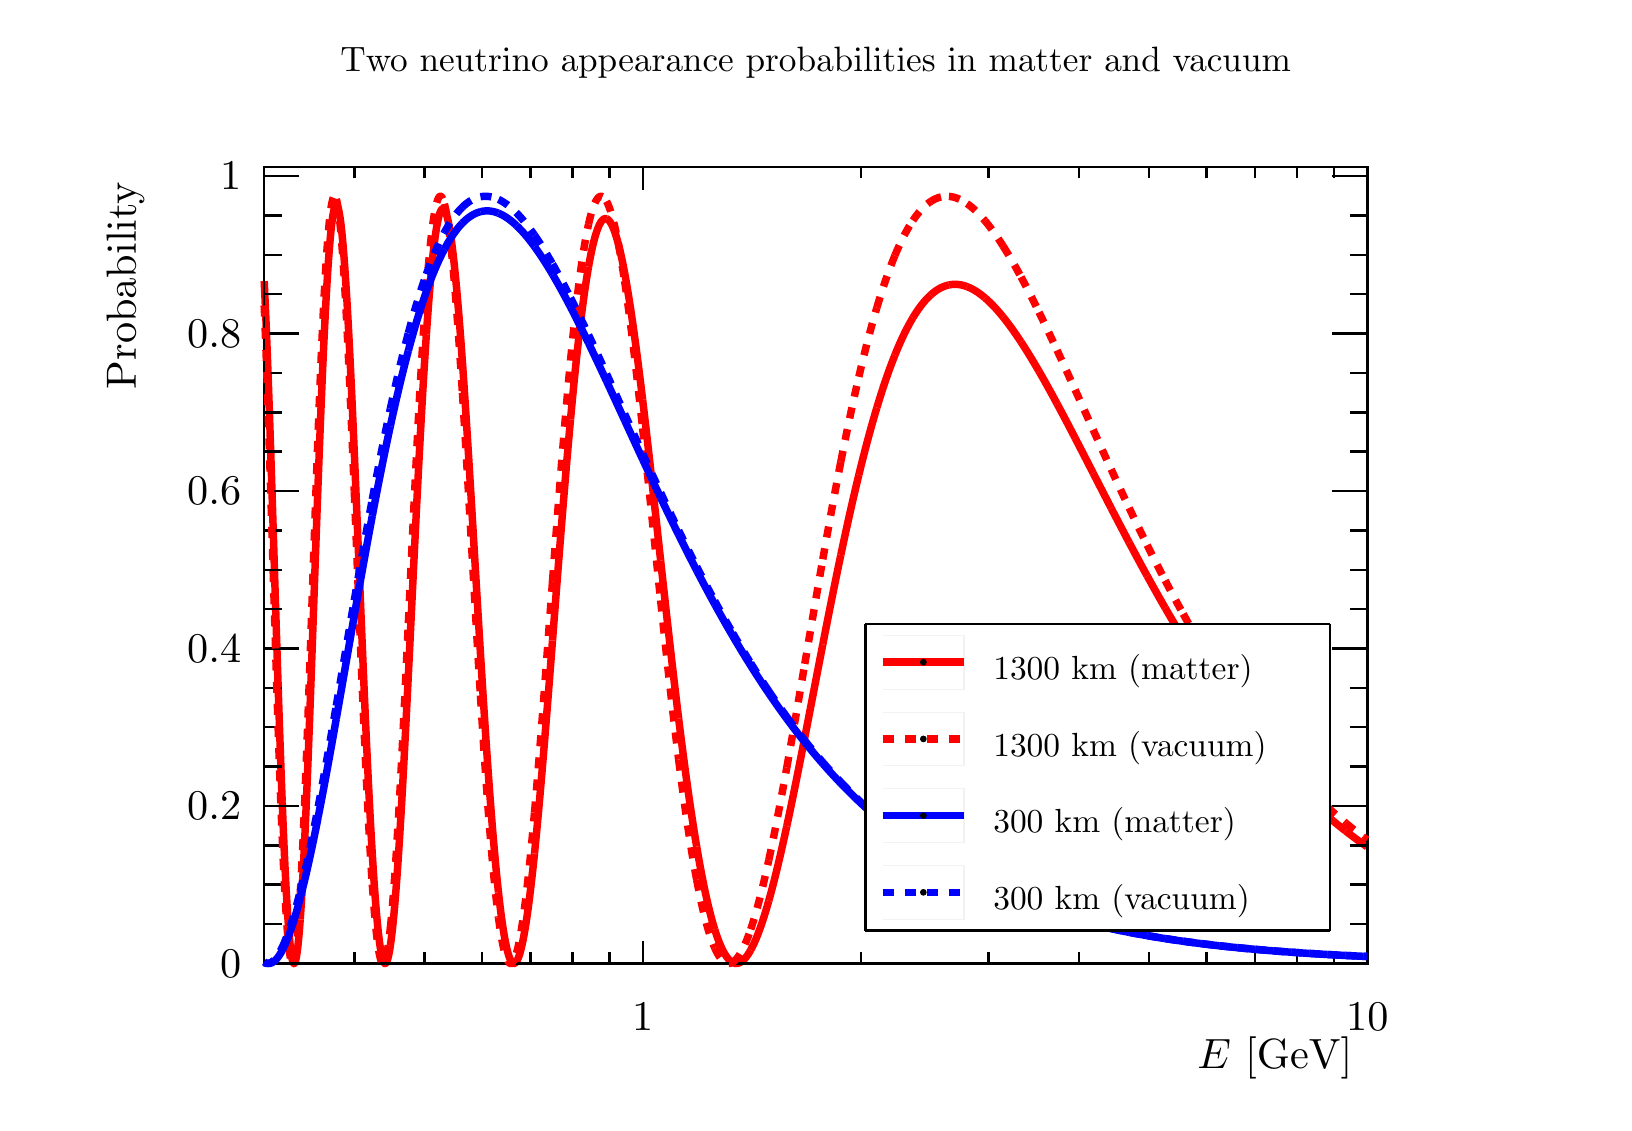
\begin{tikzpicture}
\pgfdeclareplotmark{cross} {
\pgfpathmoveto{\pgfpoint{-0.3\pgfplotmarksize}{\pgfplotmarksize}}
\pgfpathlineto{\pgfpoint{+0.3\pgfplotmarksize}{\pgfplotmarksize}}
\pgfpathlineto{\pgfpoint{+0.3\pgfplotmarksize}{0.3\pgfplotmarksize}}
\pgfpathlineto{\pgfpoint{+1\pgfplotmarksize}{0.3\pgfplotmarksize}}
\pgfpathlineto{\pgfpoint{+1\pgfplotmarksize}{-0.3\pgfplotmarksize}}
\pgfpathlineto{\pgfpoint{+0.3\pgfplotmarksize}{-0.3\pgfplotmarksize}}
\pgfpathlineto{\pgfpoint{+0.3\pgfplotmarksize}{-1.\pgfplotmarksize}}
\pgfpathlineto{\pgfpoint{-0.3\pgfplotmarksize}{-1.\pgfplotmarksize}}
\pgfpathlineto{\pgfpoint{-0.3\pgfplotmarksize}{-0.3\pgfplotmarksize}}
\pgfpathlineto{\pgfpoint{-1.\pgfplotmarksize}{-0.3\pgfplotmarksize}}
\pgfpathlineto{\pgfpoint{-1.\pgfplotmarksize}{0.3\pgfplotmarksize}}
\pgfpathlineto{\pgfpoint{-0.3\pgfplotmarksize}{0.3\pgfplotmarksize}}
\pgfpathclose
\pgfusepathqstroke
}
\pgfdeclareplotmark{cross*} {
\pgfpathmoveto{\pgfpoint{-0.3\pgfplotmarksize}{\pgfplotmarksize}}
\pgfpathlineto{\pgfpoint{+0.3\pgfplotmarksize}{\pgfplotmarksize}}
\pgfpathlineto{\pgfpoint{+0.3\pgfplotmarksize}{0.3\pgfplotmarksize}}
\pgfpathlineto{\pgfpoint{+1\pgfplotmarksize}{0.3\pgfplotmarksize}}
\pgfpathlineto{\pgfpoint{+1\pgfplotmarksize}{-0.3\pgfplotmarksize}}
\pgfpathlineto{\pgfpoint{+0.3\pgfplotmarksize}{-0.3\pgfplotmarksize}}
\pgfpathlineto{\pgfpoint{+0.3\pgfplotmarksize}{-1.\pgfplotmarksize}}
\pgfpathlineto{\pgfpoint{-0.3\pgfplotmarksize}{-1.\pgfplotmarksize}}
\pgfpathlineto{\pgfpoint{-0.3\pgfplotmarksize}{-0.3\pgfplotmarksize}}
\pgfpathlineto{\pgfpoint{-1.\pgfplotmarksize}{-0.3\pgfplotmarksize}}
\pgfpathlineto{\pgfpoint{-1.\pgfplotmarksize}{0.3\pgfplotmarksize}}
\pgfpathlineto{\pgfpoint{-0.3\pgfplotmarksize}{0.3\pgfplotmarksize}}
\pgfpathclose
\pgfusepathqfillstroke
}
\pgfdeclareplotmark{newstar} {
\pgfpathmoveto{\pgfqpoint{0pt}{\pgfplotmarksize}}
\pgfpathlineto{\pgfqpointpolar{44}{0.5\pgfplotmarksize}}
\pgfpathlineto{\pgfqpointpolar{18}{\pgfplotmarksize}}
\pgfpathlineto{\pgfqpointpolar{-20}{0.5\pgfplotmarksize}}
\pgfpathlineto{\pgfqpointpolar{-54}{\pgfplotmarksize}}
\pgfpathlineto{\pgfqpointpolar{-90}{0.5\pgfplotmarksize}}
\pgfpathlineto{\pgfqpointpolar{234}{\pgfplotmarksize}}
\pgfpathlineto{\pgfqpointpolar{198}{0.5\pgfplotmarksize}}
\pgfpathlineto{\pgfqpointpolar{162}{\pgfplotmarksize}}
\pgfpathlineto{\pgfqpointpolar{134}{0.5\pgfplotmarksize}}
\pgfpathclose
\pgfusepathqstroke
}
\pgfdeclareplotmark{newstar*} {
\pgfpathmoveto{\pgfqpoint{0pt}{\pgfplotmarksize}}
\pgfpathlineto{\pgfqpointpolar{44}{0.5\pgfplotmarksize}}
\pgfpathlineto{\pgfqpointpolar{18}{\pgfplotmarksize}}
\pgfpathlineto{\pgfqpointpolar{-20}{0.5\pgfplotmarksize}}
\pgfpathlineto{\pgfqpointpolar{-54}{\pgfplotmarksize}}
\pgfpathlineto{\pgfqpointpolar{-90}{0.5\pgfplotmarksize}}
\pgfpathlineto{\pgfqpointpolar{234}{\pgfplotmarksize}}
\pgfpathlineto{\pgfqpointpolar{198}{0.5\pgfplotmarksize}}
\pgfpathlineto{\pgfqpointpolar{162}{\pgfplotmarksize}}
\pgfpathlineto{\pgfqpointpolar{134}{0.5\pgfplotmarksize}}
\pgfpathclose
\pgfusepathqfillstroke
}
\definecolor{c}{rgb}{1,1,1};
\draw [color=c, fill=c] (0,0) rectangle (20,13.639);
\draw [color=c, fill=c] (2.99427,1.76218) rectangle (17.0057,11.8768);
\definecolor{c}{rgb}{0,0,0};
\draw [c,line width=0.9] (2.99427,1.76218) -- (2.99427,11.8768) -- (17.0057,11.8768) -- (17.0057,1.76218) -- (2.99427,1.76218);
\definecolor{c}{rgb}{1,1,1};
\draw [color=c, fill=c] (2.99427,1.76218) rectangle (17.0057,11.8768);
\definecolor{c}{rgb}{0,0,0};
\draw [c,line width=0.9] (2.99427,1.76218) -- (2.99427,11.8768) -- (17.0057,11.8768) -- (17.0057,1.76218) -- (2.99427,1.76218);
\definecolor{c}{rgb}{1,0,0};
\draw [c,line width=2.7] (2.99661,10.4272) -- (3.00128,10.331) -- (3.00595,10.231) -- (3.01062,10.1275) -- (3.01529,10.0204) -- (3.01996,9.90998) -- (3.02463,9.79629) -- (3.0293,9.67947) -- (3.03397,9.55965) -- (3.03864,9.43697) -- (3.04331,9.31155)
 -- (3.04798,9.18355) -- (3.05265,9.05308) -- (3.05732,8.92031) -- (3.06199,8.78535) -- (3.06666,8.64837) -- (3.07133,8.50949) -- (3.076,8.36887) -- (3.08067,8.22666) -- (3.08534,8.083) -- (3.09001,7.93803) -- (3.09469,7.7919) -- (3.09936,7.64477) --
 (3.10403,7.49678) -- (3.1087,7.34808) -- (3.11337,7.19882) -- (3.11804,7.04914) -- (3.12271,6.89919) -- (3.12738,6.74912) -- (3.13205,6.59907) -- (3.13672,6.44919) -- (3.14139,6.29963) -- (3.14606,6.15052) -- (3.15073,6.00201) -- (3.1554,5.85423) --
 (3.16007,5.70733) -- (3.16474,5.56145) -- (3.16941,5.41671) -- (3.17408,5.27325) -- (3.17875,5.13121) -- (3.18342,4.99071) -- (3.1881,4.85187) -- (3.19277,4.71483) -- (3.19744,4.57971) -- (3.20211,4.44662) -- (3.20678,4.31568) -- (3.21145,4.18701)
 -- (3.21612,4.06072) -- (3.22079,3.93691) -- (3.22546,3.8157);
\draw [c,line width=2.7] (3.22546,3.8157) -- (3.23013,3.69718) -- (3.2348,3.58146) -- (3.23947,3.46862) -- (3.24414,3.35878) -- (3.24881,3.252) -- (3.25348,3.14839) -- (3.25815,3.04802) -- (3.26282,2.95098) -- (3.26749,2.85733) -- (3.27216,2.76716)
 -- (3.27683,2.68053) -- (3.2815,2.5975) -- (3.28618,2.51814) -- (3.29085,2.44251) -- (3.29552,2.37066) -- (3.30019,2.30265) -- (3.30486,2.23851) -- (3.30953,2.17829) -- (3.3142,2.12203) -- (3.31887,2.06977) -- (3.32354,2.02154) -- (3.32821,1.97737)
 -- (3.33288,1.93727) -- (3.33755,1.90128) -- (3.34222,1.86941) -- (3.34689,1.84166) -- (3.35156,1.81806) -- (3.35623,1.79861) -- (3.3609,1.78331) -- (3.36557,1.77215) -- (3.37024,1.76514) -- (3.37491,1.76218) -- (3.37959,1.7635) -- (3.38426,1.76885)
 -- (3.38893,1.77828) -- (3.3936,1.79179) -- (3.39827,1.80932) -- (3.40294,1.83087) -- (3.40761,1.8564) -- (3.41228,1.88587) -- (3.41695,1.91924) -- (3.42162,1.95647) -- (3.42629,1.99752) -- (3.43096,2.04233) -- (3.43563,2.09087) -- (3.4403,2.14307)
 -- (3.44497,2.19887) -- (3.44964,2.25823) -- (3.45431,2.32107);
\draw [c,line width=2.7] (3.45431,2.32107) -- (3.45898,2.38734) -- (3.46365,2.45696) -- (3.46832,2.52987) -- (3.473,2.606) -- (3.47767,2.68527) -- (3.48234,2.76761) -- (3.48701,2.85294) -- (3.49168,2.94118) -- (3.49635,3.03225) -- (3.50102,3.12606)
 -- (3.50569,3.22253) -- (3.51036,3.32158) -- (3.51503,3.42311) -- (3.5197,3.52703) -- (3.52437,3.63326) -- (3.52904,3.7417) -- (3.53371,3.85225) -- (3.53838,3.96483) -- (3.54305,4.07934) -- (3.54772,4.19567) -- (3.55239,4.31373) -- (3.55706,4.43342)
 -- (3.56173,4.55465) -- (3.5664,4.67731) -- (3.57108,4.8013) -- (3.57575,4.92653) -- (3.58042,5.05288) -- (3.58509,5.18026) -- (3.58976,5.30857) -- (3.59443,5.4377) -- (3.5991,5.56755) -- (3.60377,5.69802) -- (3.60844,5.82901) -- (3.61311,5.96041)
 -- (3.61778,6.09213) -- (3.62245,6.22406) -- (3.62712,6.35611) -- (3.63179,6.48817) -- (3.63646,6.62014) -- (3.64113,6.75192) -- (3.6458,6.88342) -- (3.65047,7.01454) -- (3.65514,7.14518) -- (3.65981,7.27525) -- (3.66448,7.40465) --
 (3.66916,7.53328) -- (3.67383,7.66107) -- (3.6785,7.7879) -- (3.68317,7.9137);
\draw [c,line width=2.7] (3.68317,7.9137) -- (3.68784,8.03837) -- (3.69251,8.16183) -- (3.69718,8.284) -- (3.70185,8.40478) -- (3.70652,8.52409) -- (3.71119,8.64186) -- (3.71586,8.75799) -- (3.72053,8.87243) -- (3.7252,8.98508) -- (3.72987,9.09587)
 -- (3.73454,9.20474) -- (3.73921,9.3116) -- (3.74388,9.41639) -- (3.74855,9.51905) -- (3.75322,9.6195) -- (3.75789,9.71768) -- (3.76257,9.81354) -- (3.76724,9.90701) -- (3.77191,9.99803) -- (3.77658,10.0866) -- (3.78125,10.1725) -- (3.78592,10.2559)
 -- (3.79059,10.3366) -- (3.79526,10.4146) -- (3.79993,10.4899) -- (3.8046,10.5623) -- (3.80927,10.632) -- (3.81394,10.6988) -- (3.81861,10.7626) -- (3.82328,10.8236) -- (3.82795,10.8816) -- (3.83262,10.9365) -- (3.83729,10.9885) -- (3.84196,11.0374)
 -- (3.84663,11.0832) -- (3.8513,11.126) -- (3.85597,11.1656) -- (3.86065,11.2021) -- (3.86532,11.2355) -- (3.86999,11.2657) -- (3.87466,11.2928) -- (3.87933,11.3166) -- (3.884,11.3374) -- (3.88867,11.3549) -- (3.89334,11.3693) -- (3.89801,11.3805)
 -- (3.90268,11.3885) -- (3.90735,11.3934) -- (3.91202,11.3951);
\draw [c,line width=2.7] (3.91202,11.3951) -- (3.91669,11.3937) -- (3.92136,11.3892) -- (3.92603,11.3815) -- (3.9307,11.3707) -- (3.93537,11.3568) -- (3.94004,11.3399) -- (3.94471,11.3199) -- (3.94938,11.297) -- (3.95406,11.271) -- (3.95873,11.242)
 -- (3.9634,11.2101) -- (3.96807,11.1753) -- (3.97274,11.1377) -- (3.97741,11.0972) -- (3.98208,11.0538) -- (3.98675,11.0078) -- (3.99142,10.9589) -- (3.99609,10.9074) -- (4.00076,10.8533) -- (4.00543,10.7965) -- (4.0101,10.7372) -- (4.01477,10.6754)
 -- (4.01944,10.6111) -- (4.02411,10.5444) -- (4.02878,10.4753) -- (4.03345,10.4039) -- (4.03812,10.3303) -- (4.04279,10.2544) -- (4.04746,10.1764) -- (4.05214,10.0963) -- (4.05681,10.0141) -- (4.06148,9.92993) -- (4.06615,9.84385) --
 (4.07082,9.75589) -- (4.07549,9.66612) -- (4.08016,9.57461) -- (4.08483,9.4814) -- (4.0895,9.38657) -- (4.09417,9.29017) -- (4.09884,9.19228) -- (4.10351,9.09294) -- (4.10818,8.99224) -- (4.11285,8.89022) -- (4.11752,8.78696) -- (4.12219,8.68252) --
 (4.12686,8.57697) -- (4.13153,8.47038) -- (4.1362,8.3628) -- (4.14087,8.25432);
\draw [c,line width=2.7] (4.14087,8.25432) -- (4.14555,8.14498) -- (4.15022,8.03486) -- (4.15489,7.92404) -- (4.15956,7.81256) -- (4.16423,7.7005) -- (4.1689,7.58794) -- (4.17357,7.47492) -- (4.17824,7.36153) -- (4.18291,7.24782) -- (4.18758,7.13387)
 -- (4.19225,7.01973) -- (4.19692,6.90548) -- (4.20159,6.79117) -- (4.20626,6.67689) -- (4.21093,6.56268) -- (4.2156,6.44861) -- (4.22027,6.33475) -- (4.22494,6.22117) -- (4.22961,6.10791) -- (4.23428,5.99505) -- (4.23896,5.88265) --
 (4.24363,5.77076) -- (4.2483,5.65945) -- (4.25297,5.54878) -- (4.25764,5.43881) -- (4.26231,5.32959) -- (4.26698,5.22118) -- (4.27165,5.11364) -- (4.27632,5.00702) -- (4.28099,4.90138) -- (4.28566,4.79678) -- (4.29033,4.69326) -- (4.295,4.59088) --
 (4.29967,4.48969) -- (4.30434,4.38975) -- (4.30901,4.29109) -- (4.31368,4.19377) -- (4.31835,4.09783) -- (4.32302,4.00333) -- (4.32769,3.9103) -- (4.33236,3.8188) -- (4.33704,3.72886) -- (4.34171,3.64053) -- (4.34638,3.55385) -- (4.35105,3.46885) --
 (4.35572,3.38558) -- (4.36039,3.30408) -- (4.36506,3.22437) -- (4.36973,3.1465);
\draw [c,line width=2.7] (4.36973,3.1465) -- (4.3744,3.07051) -- (4.37907,2.99641) -- (4.38374,2.92425) -- (4.38841,2.85405) -- (4.39308,2.78585) -- (4.39775,2.71967) -- (4.40242,2.65554) -- (4.40709,2.59349) -- (4.41176,2.53353) -- (4.41643,2.4757)
 -- (4.4211,2.42001) -- (4.42577,2.36649) -- (4.43044,2.31515) -- (4.43512,2.26601) -- (4.43979,2.21909) -- (4.44446,2.17441) -- (4.44913,2.13198) -- (4.4538,2.09181) -- (4.45847,2.05392) -- (4.46314,2.01831) -- (4.46781,1.985) -- (4.47248,1.95399)
 -- (4.47715,1.92529) -- (4.48182,1.89891) -- (4.48649,1.87486) -- (4.49116,1.85312) -- (4.49583,1.83372) -- (4.5005,1.81665) -- (4.50517,1.8019) -- (4.50984,1.78948) -- (4.51451,1.77939) -- (4.51918,1.77162) -- (4.52385,1.76617) -- (4.52852,1.76218)
 -- (4.5332,1.76218) -- (4.53787,1.76366) -- (4.54254,1.76742) -- (4.54721,1.77345) -- (4.55188,1.78175) -- (4.55655,1.79231) -- (4.56122,1.80511) -- (4.56589,1.82014) -- (4.57056,1.83738) -- (4.57523,1.85682) -- (4.5799,1.87844) -- (4.58457,1.90223)
 -- (4.58924,1.92816) -- (4.59391,1.95621) -- (4.59858,1.98637);
\draw [c,line width=2.7] (4.59858,1.98637) -- (4.60325,2.01861) -- (4.60792,2.05291) -- (4.61259,2.08925) -- (4.61726,2.1276) -- (4.62193,2.16793) -- (4.62661,2.21023) -- (4.63128,2.25447) -- (4.63595,2.30061) -- (4.64062,2.34863) --
 (4.64529,2.39851) -- (4.64996,2.45021) -- (4.65463,2.5037) -- (4.6593,2.55896) -- (4.66397,2.61594) -- (4.66864,2.67463) -- (4.67331,2.73498) -- (4.67798,2.79697) -- (4.68265,2.86055) -- (4.68732,2.9257) -- (4.69199,2.99239) -- (4.69666,3.06057) --
 (4.70133,3.13021) -- (4.706,3.20128) -- (4.71067,3.27373) -- (4.71534,3.34754) -- (4.72002,3.42266) -- (4.72469,3.49906) -- (4.72936,3.5767) -- (4.73403,3.65553) -- (4.7387,3.73553) -- (4.74337,3.81666) -- (4.74804,3.89886) -- (4.75271,3.98211) --
 (4.75738,4.06637) -- (4.76205,4.15159) -- (4.76672,4.23774) -- (4.77139,4.32477) -- (4.77606,4.41265) -- (4.78073,4.50133) -- (4.7854,4.59077) -- (4.79007,4.68094) -- (4.79474,4.77179) -- (4.79941,4.86328) -- (4.80408,4.95537) -- (4.80875,5.04802)
 -- (4.81342,5.14119) -- (4.8181,5.23484) -- (4.82277,5.32893) -- (4.82744,5.42341);
\draw [c,line width=2.7] (4.82744,5.42341) -- (4.83211,5.51825) -- (4.83678,5.6134) -- (4.84145,5.70883) -- (4.84612,5.80449) -- (4.85079,5.90034) -- (4.85546,5.99635) -- (4.86013,6.09248) -- (4.8648,6.18868) -- (4.86947,6.28491) -- (4.87414,6.38114)
 -- (4.87881,6.47732) -- (4.88348,6.57343) -- (4.88815,6.66941) -- (4.89282,6.76523) -- (4.89749,6.86086) -- (4.90216,6.95625) -- (4.90683,7.05137) -- (4.9115,7.14618) -- (4.91618,7.24064) -- (4.92085,7.33472) -- (4.92552,7.42839) -- (4.93019,7.5216)
 -- (4.93486,7.61432) -- (4.93953,7.70651) -- (4.9442,7.79815) -- (4.94887,7.8892) -- (4.95354,7.97962) -- (4.95821,8.06938) -- (4.96288,8.15845) -- (4.96755,8.2468) -- (4.97222,8.33439) -- (4.97689,8.42119) -- (4.98156,8.50718) -- (4.98623,8.59232)
 -- (4.9909,8.67659) -- (4.99557,8.75994) -- (5.00024,8.84236) -- (5.00491,8.92382) -- (5.00959,9.00429) -- (5.01426,9.08374) -- (5.01893,9.16215) -- (5.0236,9.23948) -- (5.02827,9.31572) -- (5.03294,9.39084) -- (5.03761,9.46482) -- (5.04228,9.53762)
 -- (5.04695,9.60924) -- (5.05162,9.67964) -- (5.05629,9.74881);
\draw [c,line width=2.7] (5.05629,9.74881) -- (5.06096,9.81671) -- (5.06563,9.88335) -- (5.0703,9.94868) -- (5.07497,10.0127) -- (5.07964,10.0754) -- (5.08431,10.1367) -- (5.08898,10.1967) -- (5.09365,10.2552) -- (5.09832,10.3124) --
 (5.10299,10.3681) -- (5.10767,10.4224) -- (5.11234,10.4753) -- (5.11701,10.5267) -- (5.12168,10.5766) -- (5.12635,10.625) -- (5.13102,10.6719) -- (5.13569,10.7173) -- (5.14036,10.7612) -- (5.14503,10.8035) -- (5.1497,10.8443) -- (5.15437,10.8835) --
 (5.15904,10.9212) -- (5.16371,10.9573) -- (5.16838,10.9919) -- (5.17305,11.0248) -- (5.17772,11.0562) -- (5.18239,11.0859) -- (5.18706,11.1141) -- (5.19173,11.1406) -- (5.1964,11.1656) -- (5.20108,11.1889) -- (5.20575,11.2107) -- (5.21042,11.2308)
 -- (5.21509,11.2493) -- (5.21976,11.2661) -- (5.22443,11.2814) -- (5.2291,11.295) -- (5.23377,11.3071) -- (5.23844,11.3175) -- (5.24311,11.3263) -- (5.24778,11.3335) -- (5.25245,11.3391) -- (5.25712,11.3431) -- (5.26179,11.3455) -- (5.26646,11.3463)
 -- (5.27113,11.3455) -- (5.2758,11.3431) -- (5.28047,11.3392) -- (5.28514,11.3337);
\draw [c,line width=2.7] (5.28514,11.3337) -- (5.28981,11.3266) -- (5.29449,11.318) -- (5.29916,11.3078) -- (5.30383,11.2961) -- (5.3085,11.2829) -- (5.31317,11.2681) -- (5.31784,11.2519) -- (5.32251,11.2341) -- (5.32718,11.2149) -- (5.33185,11.1942)
 -- (5.33652,11.172) -- (5.34119,11.1484) -- (5.34586,11.1233) -- (5.35053,11.0968) -- (5.3552,11.0689) -- (5.35987,11.0397) -- (5.36454,11.009) -- (5.36921,10.977) -- (5.37388,10.9436) -- (5.37855,10.9089) -- (5.38322,10.8728) -- (5.38789,10.8355)
 -- (5.39257,10.7968) -- (5.39724,10.7569) -- (5.40191,10.7157) -- (5.40658,10.6733) -- (5.41125,10.6297) -- (5.41592,10.5849) -- (5.42059,10.5389) -- (5.42526,10.4917) -- (5.42993,10.4434) -- (5.4346,10.3939) -- (5.43927,10.3434) --
 (5.44394,10.2917) -- (5.44861,10.239) -- (5.45328,10.1852) -- (5.45795,10.1304) -- (5.46262,10.0746) -- (5.46729,10.0178) -- (5.47196,9.96001) -- (5.47663,9.90129) -- (5.4813,9.84165) -- (5.48597,9.78109) -- (5.49065,9.71966) -- (5.49532,9.65735) --
 (5.49999,9.59421) -- (5.50466,9.53025) -- (5.50933,9.46549) -- (5.514,9.39995);
\draw [c,line width=2.7] (5.514,9.39995) -- (5.51867,9.33366) -- (5.52334,9.26664) -- (5.52801,9.1989) -- (5.53268,9.13048) -- (5.53735,9.0614) -- (5.54202,8.99167) -- (5.54669,8.92132) -- (5.55136,8.85038) -- (5.55603,8.77886) -- (5.5607,8.70679) --
 (5.56537,8.63419) -- (5.57004,8.56109) -- (5.57471,8.4875) -- (5.57938,8.41345) -- (5.58405,8.33896) -- (5.58873,8.26406) -- (5.5934,8.18876) -- (5.59807,8.11309) -- (5.60274,8.03708) -- (5.60741,7.96074) -- (5.61208,7.8841) -- (5.61675,7.80718) --
 (5.62142,7.73001) -- (5.62609,7.6526) -- (5.63076,7.57498) -- (5.63543,7.49717) -- (5.6401,7.41919) -- (5.64477,7.34106) -- (5.64944,7.26282) -- (5.65411,7.18447) -- (5.65878,7.10605) -- (5.66345,7.02756) -- (5.66812,6.94904) -- (5.67279,6.87051) --
 (5.67746,6.79199) -- (5.68214,6.71349) -- (5.68681,6.63504) -- (5.69148,6.55667) -- (5.69615,6.47839) -- (5.70082,6.40021) -- (5.70549,6.32218) -- (5.71016,6.24429) -- (5.71483,6.16658) -- (5.7195,6.08907) -- (5.72417,6.01177) -- (5.72884,5.9347) --
 (5.73351,5.85789) -- (5.73818,5.78135) -- (5.74285,5.7051);
\draw [c,line width=2.7] (5.74285,5.7051) -- (5.74752,5.62916) -- (5.75219,5.55355) -- (5.75686,5.47829) -- (5.76153,5.4034) -- (5.7662,5.32889) -- (5.77087,5.25479) -- (5.77555,5.18111) -- (5.78022,5.10786) -- (5.78489,5.03507) -- (5.78956,4.96276)
 -- (5.79423,4.89093) -- (5.7989,4.81961) -- (5.80357,4.74882) -- (5.80824,4.67856) -- (5.81291,4.60886) -- (5.81758,4.53973) -- (5.82225,4.47119) -- (5.82692,4.40325) -- (5.83159,4.33592) -- (5.83626,4.26923) -- (5.84093,4.20318) -- (5.8456,4.13779)
 -- (5.85027,4.07308) -- (5.85494,4.00906) -- (5.85961,3.94573) -- (5.86428,3.88312) -- (5.86895,3.82124) -- (5.87363,3.7601) -- (5.8783,3.69971) -- (5.88297,3.64009) -- (5.88764,3.58125) -- (5.89231,3.52319) -- (5.89698,3.46593) -- (5.90165,3.40948)
 -- (5.90632,3.35386) -- (5.91099,3.29907) -- (5.91566,3.24512) -- (5.92033,3.19202) -- (5.925,3.13979) -- (5.92967,3.08842) -- (5.93434,3.03794) -- (5.93901,2.98835) -- (5.94368,2.93966) -- (5.94835,2.89187) -- (5.95302,2.845) -- (5.95769,2.79905)
 -- (5.96236,2.75404) -- (5.96704,2.70996) -- (5.97171,2.66683);
\draw [c,line width=2.7] (5.97171,2.66683) -- (5.97638,2.62464) -- (5.98105,2.58342) -- (5.98572,2.54316) -- (5.99039,2.50387) -- (5.99506,2.46556) -- (5.99973,2.42823) -- (6.0044,2.39188) -- (6.00907,2.35653) -- (6.01374,2.32217) --
 (6.01841,2.28881) -- (6.02308,2.25646) -- (6.02775,2.22512) -- (6.03242,2.19478) -- (6.03709,2.16547) -- (6.04176,2.13717) -- (6.04643,2.10989) -- (6.0511,2.08363) -- (6.05577,2.0584) -- (6.06044,2.0342) -- (6.06512,2.01103) -- (6.06979,1.98889) --
 (6.07446,1.96778) -- (6.07913,1.9477) -- (6.0838,1.92866) -- (6.08847,1.91065) -- (6.09314,1.89368) -- (6.09781,1.87774) -- (6.10248,1.86284) -- (6.10715,1.84897) -- (6.11182,1.83614) -- (6.11649,1.82433) -- (6.12116,1.81356) -- (6.12583,1.80382) --
 (6.1305,1.79511) -- (6.13517,1.78742) -- (6.13984,1.78076) -- (6.14451,1.77513) -- (6.14918,1.77051) -- (6.15385,1.76691) -- (6.15852,1.76432) -- (6.1632,1.76218) -- (6.16787,1.76218) -- (6.17254,1.76218) -- (6.17721,1.76406) -- (6.18188,1.76649) --
 (6.18655,1.76992) -- (6.19122,1.77434) -- (6.19589,1.77974) -- (6.20056,1.78612);
\draw [c,line width=2.7] (6.20056,1.78612) -- (6.20523,1.79348) -- (6.2099,1.8018) -- (6.21457,1.81109) -- (6.21924,1.82134) -- (6.22391,1.83255) -- (6.22858,1.8447) -- (6.23325,1.85779) -- (6.23792,1.87181) -- (6.24259,1.88677) -- (6.24726,1.90265)
 -- (6.25194,1.91944) -- (6.25661,1.93715) -- (6.26128,1.95576) -- (6.26595,1.97526) -- (6.27062,1.99565) -- (6.27529,2.01693) -- (6.27996,2.03907) -- (6.28463,2.06208) -- (6.2893,2.08596) -- (6.29397,2.11068) -- (6.29864,2.13624) --
 (6.30331,2.16264) -- (6.30798,2.18986) -- (6.31265,2.2179) -- (6.31732,2.24675) -- (6.32199,2.2764) -- (6.32666,2.30684) -- (6.33133,2.33807) -- (6.336,2.37007) -- (6.34067,2.40283) -- (6.34534,2.43635) -- (6.35002,2.47061) -- (6.35469,2.50562) --
 (6.35936,2.54135) -- (6.36403,2.57779) -- (6.3687,2.61495) -- (6.37337,2.6528) -- (6.37804,2.69134) -- (6.38271,2.73056) -- (6.38738,2.77045) -- (6.39205,2.811) -- (6.39672,2.8522) -- (6.40139,2.89403) -- (6.40606,2.9365) -- (6.41073,2.97958) --
 (6.4154,3.02326) -- (6.42007,3.06755) -- (6.42474,3.11242) -- (6.42941,3.15787);
\draw [c,line width=2.7] (6.42941,3.15787) -- (6.43408,3.20388) -- (6.43875,3.25044) -- (6.44342,3.29756) -- (6.4481,3.3452) -- (6.45277,3.39336) -- (6.45744,3.44204) -- (6.46211,3.49122) -- (6.46678,3.54089) -- (6.47145,3.59103) -- (6.47612,3.64165)
 -- (6.48079,3.69272) -- (6.48546,3.74423) -- (6.49013,3.79619) -- (6.4948,3.84856) -- (6.49947,3.90135) -- (6.50414,3.95454) -- (6.50881,4.00812) -- (6.51348,4.06208) -- (6.51815,4.1164) -- (6.52282,4.17109) -- (6.52749,4.22612) -- (6.53216,4.28149)
 -- (6.53683,4.33718) -- (6.5415,4.39318) -- (6.54618,4.44948) -- (6.55085,4.50608) -- (6.55552,4.56295) -- (6.56019,4.6201) -- (6.56486,4.6775) -- (6.56953,4.73515) -- (6.5742,4.79303) -- (6.57887,4.85114) -- (6.58354,4.90946) -- (6.58821,4.96798)
 -- (6.59288,5.02669) -- (6.59755,5.08559) -- (6.60222,5.14466) -- (6.60689,5.20388) -- (6.61156,5.26326) -- (6.61623,5.32277) -- (6.6209,5.3824) -- (6.62557,5.44216) -- (6.63024,5.50202) -- (6.63491,5.56197) -- (6.63959,5.62201) -- (6.64426,5.68213)
 -- (6.64893,5.7423) -- (6.6536,5.80253) -- (6.65827,5.86281);
\draw [c,line width=2.7] (6.65827,5.86281) -- (6.66294,5.92311) -- (6.66761,5.98344) -- (6.67228,6.04378) -- (6.67695,6.10412) -- (6.68162,6.16446) -- (6.68629,6.22477) -- (6.69096,6.28506) -- (6.69563,6.34531) -- (6.7003,6.40551) --
 (6.70497,6.46566) -- (6.70964,6.52574) -- (6.71431,6.58574) -- (6.71898,6.64566) -- (6.72365,6.70548) -- (6.72832,6.76519) -- (6.733,6.82479) -- (6.73767,6.88427) -- (6.74234,6.94361) -- (6.74701,7.00282) -- (6.75168,7.06187) -- (6.75635,7.12076) --
 (6.76102,7.17948) -- (6.76569,7.23803) -- (6.77036,7.29639) -- (6.77503,7.35455) -- (6.7797,7.41252) -- (6.78437,7.47026) -- (6.78904,7.52779) -- (6.79371,7.5851) -- (6.79838,7.64216) -- (6.80305,7.69898) -- (6.80772,7.75555) -- (6.81239,7.81185) --
 (6.81706,7.86789) -- (6.82173,7.92365) -- (6.8264,7.97913) -- (6.83108,8.03432) -- (6.83575,8.0892) -- (6.84042,8.14378) -- (6.84509,8.19805) -- (6.84976,8.252) -- (6.85443,8.30562) -- (6.8591,8.3589) -- (6.86377,8.41184) -- (6.86844,8.46443) --
 (6.87311,8.51667) -- (6.87778,8.56854) -- (6.88245,8.62005) -- (6.88712,8.67118);
\draw [c,line width=2.7] (6.88712,8.67118) -- (6.89179,8.72193) -- (6.89646,8.77229) -- (6.90113,8.82226) -- (6.9058,8.87183) -- (6.91047,8.92099) -- (6.91514,8.96974) -- (6.91981,9.01808) -- (6.92448,9.06599) -- (6.92916,9.11347) --
 (6.93383,9.16052) -- (6.9385,9.20713) -- (6.94317,9.25329) -- (6.94784,9.29901) -- (6.95251,9.34427) -- (6.95718,9.38906) -- (6.96185,9.4334) -- (6.96652,9.47726) -- (6.97119,9.52066) -- (6.97586,9.56357) -- (6.98053,9.606) -- (6.9852,9.64794) --
 (6.98987,9.68939) -- (6.99454,9.73034) -- (6.99921,9.7708) -- (7.00388,9.81075) -- (7.00855,9.85019) -- (7.01322,9.88912) -- (7.01789,9.92753) -- (7.02257,9.96543) -- (7.02724,10.0028) -- (7.03191,10.0397) -- (7.03658,10.076) -- (7.04125,10.1118) --
 (7.04592,10.147) -- (7.05059,10.1817) -- (7.05526,10.2159) -- (7.05993,10.2495) -- (7.0646,10.2826) -- (7.06927,10.3151) -- (7.07394,10.3471) -- (7.07861,10.3785) -- (7.08328,10.4094) -- (7.08795,10.4397) -- (7.09262,10.4695) -- (7.09729,10.4987) --
 (7.10196,10.5273) -- (7.10663,10.5553) -- (7.1113,10.5828) -- (7.11597,10.6097);
\draw [c,line width=2.7] (7.11597,10.6097) -- (7.12065,10.6361) -- (7.12532,10.6619) -- (7.12999,10.6871) -- (7.13466,10.7117) -- (7.13933,10.7357) -- (7.144,10.7592) -- (7.14867,10.7821) -- (7.15334,10.8044) -- (7.15801,10.8261) -- (7.16268,10.8472)
 -- (7.16735,10.8678) -- (7.17202,10.8878) -- (7.17669,10.9072) -- (7.18136,10.926) -- (7.18603,10.9442) -- (7.1907,10.9618) -- (7.19537,10.9789) -- (7.20004,10.9954) -- (7.20471,11.0113) -- (7.20938,11.0266) -- (7.21406,11.0413) -- (7.21873,11.0554)
 -- (7.2234,11.0689) -- (7.22807,11.0819) -- (7.23274,11.0943) -- (7.23741,11.1061) -- (7.24208,11.1173) -- (7.24675,11.1279) -- (7.25142,11.1379) -- (7.25609,11.1474) -- (7.26076,11.1563) -- (7.26543,11.1646) -- (7.2701,11.1723) -- (7.27477,11.1795)
 -- (7.27944,11.1861) -- (7.28411,11.1921) -- (7.28878,11.1975) -- (7.29345,11.2023) -- (7.29812,11.2066) -- (7.30279,11.2104) -- (7.30747,11.2135) -- (7.31214,11.2161) -- (7.31681,11.2181) -- (7.32148,11.2196) -- (7.32615,11.2205) --
 (7.33082,11.2208) -- (7.33549,11.2206) -- (7.34016,11.2198) -- (7.34483,11.2185);
\draw [c,line width=2.7] (7.34483,11.2185) -- (7.3495,11.2166) -- (7.35417,11.2142) -- (7.35884,11.2113) -- (7.36351,11.2078) -- (7.36818,11.2037) -- (7.37285,11.1991) -- (7.37752,11.194) -- (7.38219,11.1883) -- (7.38686,11.1821) -- (7.39153,11.1754)
 -- (7.3962,11.1682) -- (7.40087,11.1604) -- (7.40555,11.1521) -- (7.41022,11.1433) -- (7.41489,11.134) -- (7.41956,11.1242) -- (7.42423,11.1138) -- (7.4289,11.103) -- (7.43357,11.0916) -- (7.43824,11.0798) -- (7.44291,11.0674) -- (7.44758,11.0546)
 -- (7.45225,11.0413) -- (7.45692,11.0275) -- (7.46159,11.0132) -- (7.46626,10.9984) -- (7.47093,10.9831) -- (7.4756,10.9674) -- (7.48027,10.9512) -- (7.48494,10.9345) -- (7.48961,10.9174) -- (7.49428,10.8998) -- (7.49895,10.8818) --
 (7.50363,10.8633) -- (7.5083,10.8443) -- (7.51297,10.8249) -- (7.51764,10.8051) -- (7.52231,10.7848) -- (7.52698,10.7641) -- (7.53165,10.743) -- (7.53632,10.7214) -- (7.54099,10.6994) -- (7.54566,10.677) -- (7.55033,10.6542) -- (7.555,10.631) --
 (7.55967,10.6073) -- (7.56434,10.5833) -- (7.56901,10.5589) -- (7.57368,10.534);
\draw [c,line width=2.7] (7.57368,10.534) -- (7.57835,10.5088) -- (7.58302,10.4832) -- (7.58769,10.4572) -- (7.59236,10.4309) -- (7.59703,10.4041) -- (7.60171,10.377) -- (7.60638,10.3495) -- (7.61105,10.3217) -- (7.61572,10.2935) -- (7.62039,10.2649)
 -- (7.62506,10.236) -- (7.62973,10.2068) -- (7.6344,10.1772) -- (7.63907,10.1473) -- (7.64374,10.1171) -- (7.64841,10.0865) -- (7.65308,10.0556) -- (7.65775,10.0244) -- (7.66242,9.99282) -- (7.66709,9.96097) -- (7.67176,9.92882) -- (7.67643,9.89637)
 -- (7.6811,9.86362) -- (7.68577,9.83058) -- (7.69044,9.79725) -- (7.69512,9.76364) -- (7.69979,9.72974) -- (7.70446,9.69557) -- (7.70913,9.66113) -- (7.7138,9.62643) -- (7.71847,9.59146) -- (7.72314,9.55624) -- (7.72781,9.52076) -- (7.73248,9.48503)
 -- (7.73715,9.44906) -- (7.74182,9.41285) -- (7.74649,9.3764) -- (7.75116,9.33972) -- (7.75583,9.30282) -- (7.7605,9.26569) -- (7.76517,9.22835) -- (7.76984,9.19079) -- (7.77451,9.15302) -- (7.77918,9.11505) -- (7.78385,9.07688) -- (7.78853,9.03851)
 -- (7.7932,8.99995) -- (7.79787,8.96121) -- (7.80254,8.92228);
\draw [c,line width=2.7] (7.80254,8.92228) -- (7.80721,8.88317) -- (7.81188,8.84389) -- (7.81655,8.80444) -- (7.82122,8.76482) -- (7.82589,8.72505) -- (7.83056,8.68511) -- (7.83523,8.64503) -- (7.8399,8.6048) -- (7.84457,8.56442) -- (7.84924,8.5239)
 -- (7.85391,8.48325) -- (7.85858,8.44247) -- (7.86325,8.40156) -- (7.86792,8.36053) -- (7.87259,8.31938) -- (7.87726,8.27812) -- (7.88193,8.23674) -- (7.88661,8.19526) -- (7.89128,8.15368) -- (7.89595,8.11201) -- (7.90062,8.07024) --
 (7.90529,8.02838) -- (7.90996,7.98643) -- (7.91463,7.94441) -- (7.9193,7.90231) -- (7.92397,7.86013) -- (7.92864,7.81789) -- (7.93331,7.77558) -- (7.93798,7.73322) -- (7.94265,7.69079) -- (7.94732,7.64832) -- (7.95199,7.60579) -- (7.95666,7.56322)
 -- (7.96133,7.52061) -- (7.966,7.47797) -- (7.97067,7.43529) -- (7.97534,7.39258) -- (7.98001,7.34984) -- (7.98469,7.30709) -- (7.98936,7.26432) -- (7.99403,7.22153) -- (7.9987,7.17873) -- (8.00337,7.13593) -- (8.00804,7.09313) -- (8.01271,7.05032)
 -- (8.01738,7.00752) -- (8.02205,6.96473) -- (8.02672,6.92196) -- (8.03139,6.87919);
\draw [c,line width=2.7] (8.03139,6.87919) -- (8.03606,6.83645) -- (8.04073,6.79373) -- (8.0454,6.75104) -- (8.05007,6.70837) -- (8.05474,6.66574) -- (8.05941,6.62315) -- (8.06408,6.5806) -- (8.06875,6.53809) -- (8.07342,6.49562) -- (8.0781,6.45321)
 -- (8.08277,6.41086) -- (8.08744,6.36856) -- (8.09211,6.32632) -- (8.09678,6.28414) -- (8.10145,6.24203) -- (8.10612,6.19999) -- (8.11079,6.15803) -- (8.11546,6.11614) -- (8.12013,6.07433) -- (8.1248,6.03261) -- (8.12947,5.99097) --
 (8.13414,5.94942) -- (8.13881,5.90796) -- (8.14348,5.8666) -- (8.14815,5.82533) -- (8.15282,5.78417) -- (8.15749,5.74311) -- (8.16216,5.70216) -- (8.16683,5.66131) -- (8.1715,5.62058) -- (8.17618,5.57997) -- (8.18085,5.53947) -- (8.18552,5.4991) --
 (8.19019,5.45885) -- (8.19486,5.41873) -- (8.19953,5.37873) -- (8.2042,5.33887) -- (8.20887,5.29914) -- (8.21354,5.25955) -- (8.21821,5.2201) -- (8.22288,5.18079) -- (8.22755,5.14163) -- (8.23222,5.10261) -- (8.23689,5.06375) -- (8.24156,5.02503) --
 (8.24623,4.98648) -- (8.2509,4.94807) -- (8.25557,4.90983) -- (8.26024,4.87175);
\draw [c,line width=2.7] (8.26024,4.87175) -- (8.26491,4.83384) -- (8.26959,4.79609) -- (8.27426,4.75851) -- (8.27893,4.7211) -- (8.2836,4.68387) -- (8.28827,4.64681) -- (8.29294,4.60992) -- (8.29761,4.57322) -- (8.30228,4.5367) -- (8.30695,4.50036)
 -- (8.31162,4.46421) -- (8.31629,4.42825) -- (8.32096,4.39248) -- (8.32563,4.35689) -- (8.3303,4.32151) -- (8.33497,4.28631) -- (8.33964,4.25132) -- (8.34431,4.21653) -- (8.34898,4.18193) -- (8.35365,4.14754) -- (8.35832,4.11336) -- (8.363,4.07938)
 -- (8.36767,4.04561) -- (8.37234,4.01204) -- (8.37701,3.97869) -- (8.38168,3.94556) -- (8.38635,3.91264) -- (8.39102,3.87993) -- (8.39569,3.84745) -- (8.40036,3.81518) -- (8.40503,3.78313) -- (8.4097,3.75131) -- (8.41437,3.71971) --
 (8.41904,3.68833) -- (8.42371,3.65719) -- (8.42838,3.62627) -- (8.43305,3.59558) -- (8.43772,3.56512) -- (8.44239,3.53489) -- (8.44706,3.50489) -- (8.45173,3.47513) -- (8.4564,3.44561) -- (8.46107,3.41632) -- (8.46575,3.38727) -- (8.47042,3.35846)
 -- (8.47509,3.32989) -- (8.47976,3.30157) -- (8.48443,3.27348) -- (8.4891,3.24564);
\draw [c,line width=2.7] (8.4891,3.24564) -- (8.49377,3.21804) -- (8.49844,3.19069) -- (8.50311,3.16358) -- (8.50778,3.13673) -- (8.51245,3.11012) -- (8.51712,3.08375) -- (8.52179,3.05764) -- (8.52646,3.03178) -- (8.53113,3.00618) -- (8.5358,2.98082)
 -- (8.54047,2.95572) -- (8.54514,2.93087) -- (8.54981,2.90628) -- (8.55449,2.88194) -- (8.55916,2.85786) -- (8.56383,2.83403) -- (8.5685,2.81046) -- (8.57317,2.78715) -- (8.57784,2.7641) -- (8.58251,2.74131) -- (8.58718,2.71878) -- (8.59185,2.69651)
 -- (8.59652,2.67449) -- (8.60119,2.65274) -- (8.60586,2.63125) -- (8.61053,2.61003) -- (8.6152,2.58906) -- (8.61987,2.56836) -- (8.62454,2.54792) -- (8.62921,2.52775) -- (8.63388,2.50784) -- (8.63855,2.48819) -- (8.64322,2.46881) --
 (8.64789,2.44969) -- (8.65257,2.43083) -- (8.65724,2.41225) -- (8.66191,2.39392) -- (8.66658,2.37587) -- (8.67125,2.35807) -- (8.67592,2.34055) -- (8.68059,2.32329) -- (8.68526,2.30629) -- (8.68993,2.28956) -- (8.6946,2.2731) -- (8.69927,2.2569) --
 (8.70394,2.24097) -- (8.70861,2.22531) -- (8.71328,2.20991) -- (8.71795,2.19478);
\draw [c,line width=2.7] (8.71795,2.19478) -- (8.72262,2.17991) -- (8.72729,2.16531) -- (8.73196,2.15098) -- (8.73663,2.13691) -- (8.7413,2.12311) -- (8.74597,2.10957) -- (8.75065,2.0963) -- (8.75532,2.08329) -- (8.75999,2.07055) -- (8.76466,2.05807)
 -- (8.76933,2.04586) -- (8.774,2.03391) -- (8.77867,2.02223) -- (8.78334,2.0108) -- (8.78801,1.99965) -- (8.79268,1.98875) -- (8.79735,1.97812) -- (8.80202,1.96775) -- (8.80669,1.95764) -- (8.81136,1.94779) -- (8.81603,1.93821) -- (8.8207,1.92888)
 -- (8.82537,1.91982) -- (8.83004,1.91102) -- (8.83471,1.90247) -- (8.83939,1.89419) -- (8.84406,1.88616) -- (8.84873,1.87839) -- (8.8534,1.87088) -- (8.85807,1.86362) -- (8.86274,1.85663) -- (8.86741,1.84988) -- (8.87208,1.8434) -- (8.87675,1.83716)
 -- (8.88142,1.83119) -- (8.88609,1.82546) -- (8.89076,1.81999) -- (8.89543,1.81477) -- (8.9001,1.8098) -- (8.90477,1.80508) -- (8.90944,1.80062) -- (8.91411,1.7964) -- (8.91878,1.79243) -- (8.92345,1.78871) -- (8.92812,1.78524) -- (8.93279,1.78201)
 -- (8.93746,1.77903) -- (8.94214,1.7763) -- (8.94681,1.77381);
\draw [c,line width=2.7] (8.94681,1.77381) -- (8.95148,1.77156) -- (8.95615,1.76956) -- (8.96082,1.7678) -- (8.96549,1.76628) -- (8.97016,1.765) -- (8.97483,1.76396) -- (8.9795,1.76218) -- (8.98417,1.76218) -- (8.98884,1.76218) -- (8.99351,1.76218)
 -- (8.99818,1.76218) -- (9.00285,1.76218) -- (9.00752,1.76332) -- (9.01219,1.76416) -- (9.01686,1.76524) -- (9.02153,1.76655) -- (9.0262,1.76809) -- (9.03087,1.76986) -- (9.03555,1.77185) -- (9.04022,1.77407) -- (9.04489,1.77652) -- (9.04956,1.7792)
 -- (9.05423,1.78209) -- (9.0589,1.78521) -- (9.06357,1.78856) -- (9.06824,1.79212) -- (9.07291,1.7959) -- (9.07758,1.79991) -- (9.08225,1.80413) -- (9.08692,1.80856) -- (9.09159,1.81322) -- (9.09626,1.81809) -- (9.10093,1.82317) -- (9.1056,1.82846)
 -- (9.11027,1.83397) -- (9.11494,1.83969) -- (9.11961,1.84561) -- (9.12428,1.85175) -- (9.12895,1.85809) -- (9.13363,1.86464) -- (9.1383,1.87139) -- (9.14297,1.87835) -- (9.14764,1.88551) -- (9.15231,1.89287) -- (9.15698,1.90043) --
 (9.16165,1.90819) -- (9.16632,1.91615) -- (9.17099,1.92431) -- (9.17566,1.93266);
\draw [c,line width=2.7] (9.17566,1.93266) -- (9.18033,1.94121) -- (9.185,1.94995) -- (9.18967,1.95888) -- (9.19434,1.96801) -- (9.19901,1.97733) -- (9.20368,1.98683) -- (9.20835,1.99652) -- (9.21302,2.0064) -- (9.21769,2.01646) -- (9.22236,2.02671)
 -- (9.22704,2.03714) -- (9.23171,2.04776) -- (9.23638,2.05855) -- (9.24105,2.06953) -- (9.24572,2.08068) -- (9.25039,2.09201) -- (9.25506,2.10351) -- (9.25973,2.11519) -- (9.2644,2.12704) -- (9.26907,2.13906) -- (9.27374,2.15126) --
 (9.27841,2.16362) -- (9.28308,2.17616) -- (9.28775,2.18886) -- (9.29242,2.20172) -- (9.29709,2.21475) -- (9.30176,2.22795) -- (9.30643,2.24131) -- (9.3111,2.25482) -- (9.31577,2.2685) -- (9.32045,2.28234) -- (9.32512,2.29633) -- (9.32979,2.31048) --
 (9.33446,2.32478) -- (9.33913,2.33924) -- (9.3438,2.35385) -- (9.34847,2.36861) -- (9.35314,2.38352) -- (9.35781,2.39858) -- (9.36248,2.41378) -- (9.36715,2.42914) -- (9.37182,2.44463) -- (9.37649,2.46027) -- (9.38116,2.47605) -- (9.38583,2.49198)
 -- (9.3905,2.50804) -- (9.39517,2.52424) -- (9.39984,2.54058) -- (9.40451,2.55705);
\draw [c,line width=2.7] (9.40451,2.55705) -- (9.40918,2.57366) -- (9.41385,2.5904) -- (9.41852,2.60728) -- (9.4232,2.62428) -- (9.42787,2.64142) -- (9.43254,2.65868) -- (9.43721,2.67607) -- (9.44188,2.69358) -- (9.44655,2.71123) -- (9.45122,2.72899)
 -- (9.45589,2.74687) -- (9.46056,2.76488) -- (9.46523,2.78301) -- (9.4699,2.80125) -- (9.47457,2.81961) -- (9.47924,2.83809) -- (9.48391,2.85668) -- (9.48858,2.87538) -- (9.49325,2.8942) -- (9.49792,2.91313) -- (9.50259,2.93217) -- (9.50726,2.95131)
 -- (9.51194,2.97056) -- (9.51661,2.98992) -- (9.52128,3.00938) -- (9.52595,3.02895) -- (9.53062,3.04862) -- (9.53529,3.06839) -- (9.53996,3.08826) -- (9.54463,3.10823) -- (9.5493,3.12829) -- (9.55397,3.14845) -- (9.55864,3.16871) --
 (9.56331,3.18906) -- (9.56798,3.2095) -- (9.57265,3.23003) -- (9.57732,3.25065) -- (9.58199,3.27136) -- (9.58666,3.29216) -- (9.59133,3.31305) -- (9.596,3.33402) -- (9.60067,3.35507) -- (9.60534,3.37621) -- (9.61001,3.39743) -- (9.61469,3.41873) --
 (9.61936,3.4401) -- (9.62403,3.46156) -- (9.6287,3.48309) -- (9.63337,3.5047);
\draw [c,line width=2.7] (9.63337,3.5047) -- (9.63804,3.52638) -- (9.64271,3.54814) -- (9.64738,3.56997) -- (9.65205,3.59187) -- (9.65672,3.61384) -- (9.66139,3.63587) -- (9.66606,3.65798) -- (9.67073,3.68015) -- (9.6754,3.70239) -- (9.68007,3.72469)
 -- (9.68474,3.74705) -- (9.68941,3.76948) -- (9.69408,3.79196) -- (9.69875,3.81451) -- (9.70342,3.83711) -- (9.7081,3.85977) -- (9.71277,3.88249) -- (9.71744,3.90526) -- (9.72211,3.92809) -- (9.72678,3.95097) -- (9.73145,3.9739) -- (9.73612,3.99688)
 -- (9.74079,4.01991) -- (9.74546,4.04299) -- (9.75013,4.06612) -- (9.7548,4.08929) -- (9.75947,4.11251) -- (9.76414,4.13577) -- (9.76881,4.15908) -- (9.77348,4.18243) -- (9.77815,4.20581) -- (9.78282,4.22924) -- (9.78749,4.25271) --
 (9.79216,4.27621) -- (9.79683,4.29976) -- (9.80151,4.32333) -- (9.80618,4.34695) -- (9.81085,4.37059) -- (9.81552,4.39427) -- (9.82019,4.41798) -- (9.82486,4.44172) -- (9.82953,4.46549) -- (9.8342,4.48929) -- (9.83887,4.51311) -- (9.84354,4.53697)
 -- (9.84821,4.56084) -- (9.85288,4.58475) -- (9.85755,4.60867) -- (9.86222,4.63262);
\draw [c,line width=2.7] (9.86222,4.63262) -- (9.86689,4.65659) -- (9.87156,4.68058) -- (9.87623,4.70459) -- (9.8809,4.72862) -- (9.88557,4.75267) -- (9.89024,4.77673) -- (9.89491,4.80081) -- (9.89958,4.82491) -- (9.90426,4.84902) --
 (9.90893,4.87314) -- (9.9136,4.89727) -- (9.91827,4.92142) -- (9.92294,4.94557) -- (9.92761,4.96974) -- (9.93228,4.99391) -- (9.93695,5.01809) -- (9.94162,5.04228) -- (9.94629,5.06647) -- (9.95096,5.09067) -- (9.95563,5.11487) -- (9.9603,5.13907) --
 (9.96497,5.16328) -- (9.96964,5.18749) -- (9.97431,5.2117) -- (9.97898,5.23591) -- (9.98365,5.26011) -- (9.98832,5.28432) -- (9.993,5.30852) -- (9.99767,5.33272) -- (10.0023,5.35691) -- (10.007,5.3811) -- (10.0117,5.40528) -- (10.0163,5.42946) --
 (10.021,5.45362) -- (10.0257,5.47778) -- (10.0304,5.50193) -- (10.035,5.52607) -- (10.0397,5.55019) -- (10.0444,5.57431) -- (10.049,5.59841) -- (10.0537,5.6225) -- (10.0584,5.64657) -- (10.0631,5.67063) -- (10.0677,5.69468) -- (10.0724,5.7187) --
 (10.0771,5.74271) -- (10.0817,5.76671) -- (10.0864,5.79068) -- (10.0911,5.81463);
\draw [c,line width=2.7] (10.0911,5.81463) -- (10.0957,5.83856) -- (10.1004,5.86248) -- (10.1051,5.88637) -- (10.1098,5.91023) -- (10.1144,5.93408) -- (10.1191,5.9579) -- (10.1238,5.98169) -- (10.1284,6.00547) -- (10.1331,6.02921) --
 (10.1378,6.05293) -- (10.1425,6.07662) -- (10.1471,6.10028) -- (10.1518,6.12391) -- (10.1565,6.14752) -- (10.1611,6.17109) -- (10.1658,6.19464) -- (10.1705,6.21815) -- (10.1751,6.24163) -- (10.1798,6.26508) -- (10.1845,6.28849) -- (10.1892,6.31187)
 -- (10.1938,6.33522) -- (10.1985,6.35853) -- (10.2032,6.3818) -- (10.2078,6.40504) -- (10.2125,6.42824) -- (10.2172,6.4514) -- (10.2218,6.47453) -- (10.2265,6.49761) -- (10.2312,6.52066) -- (10.2359,6.54367) -- (10.2405,6.56663) -- (10.2452,6.58956)
 -- (10.2499,6.61244) -- (10.2545,6.63528) -- (10.2592,6.65808) -- (10.2639,6.68083) -- (10.2686,6.70354) -- (10.2732,6.72621) -- (10.2779,6.74883) -- (10.2826,6.7714) -- (10.2872,6.79393) -- (10.2919,6.81641) -- (10.2966,6.83885) --
 (10.3012,6.86124) -- (10.3059,6.88357) -- (10.3106,6.90587) -- (10.3153,6.92811) -- (10.3199,6.9503);
\draw [c,line width=2.7] (10.3199,6.9503) -- (10.3246,6.97244) -- (10.3293,6.99453) -- (10.3339,7.01657) -- (10.3386,7.03855) -- (10.3433,7.06049) -- (10.348,7.08237) -- (10.3526,7.1042) -- (10.3573,7.12597) -- (10.362,7.14769) -- (10.3666,7.16936)
 -- (10.3713,7.19097) -- (10.376,7.21253) -- (10.3806,7.23403) -- (10.3853,7.25547) -- (10.39,7.27686) -- (10.3947,7.29819) -- (10.3993,7.31946) -- (10.404,7.34068) -- (10.4087,7.36183) -- (10.4133,7.38293) -- (10.418,7.40397) -- (10.4227,7.42495) --
 (10.4274,7.44587) -- (10.432,7.46673) -- (10.4367,7.48752) -- (10.4414,7.50826) -- (10.446,7.52893) -- (10.4507,7.54955) -- (10.4554,7.5701) -- (10.46,7.59059) -- (10.4647,7.61101) -- (10.4694,7.63137) -- (10.4741,7.65167) -- (10.4787,7.6719) --
 (10.4834,7.69207) -- (10.4881,7.71218) -- (10.4927,7.73222) -- (10.4974,7.75219) -- (10.5021,7.7721) -- (10.5067,7.79194) -- (10.5114,7.81172) -- (10.5161,7.83143) -- (10.5208,7.85107) -- (10.5254,7.87064) -- (10.5301,7.89015) -- (10.5348,7.90959)
 -- (10.5394,7.92896) -- (10.5441,7.94827) -- (10.5488,7.9675);
\draw [c,line width=2.7] (10.5488,7.9675) -- (10.5535,7.98666) -- (10.5581,8.00576) -- (10.5628,8.02479) -- (10.5675,8.04374) -- (10.5721,8.06263) -- (10.5768,8.08144) -- (10.5815,8.10019) -- (10.5861,8.11886) -- (10.5908,8.13746) -- (10.5955,8.156)
 -- (10.6002,8.17445) -- (10.6048,8.19284) -- (10.6095,8.21116) -- (10.6142,8.2294) -- (10.6188,8.24757) -- (10.6235,8.26567) -- (10.6282,8.2837) -- (10.6329,8.30165) -- (10.6375,8.31952) -- (10.6422,8.33733) -- (10.6469,8.35506) -- (10.6515,8.37272)
 -- (10.6562,8.3903) -- (10.6609,8.40781) -- (10.6655,8.42524) -- (10.6702,8.4426) -- (10.6749,8.45988) -- (10.6796,8.47709) -- (10.6842,8.49422) -- (10.6889,8.51128) -- (10.6936,8.52826) -- (10.6982,8.54516) -- (10.7029,8.56199) -- (10.7076,8.57874)
 -- (10.7122,8.59542) -- (10.7169,8.61202) -- (10.7216,8.62854) -- (10.7263,8.64499) -- (10.7309,8.66136) -- (10.7356,8.67765) -- (10.7403,8.69387) -- (10.7449,8.71) -- (10.7496,8.72606) -- (10.7543,8.74205) -- (10.759,8.75795) -- (10.7636,8.77378)
 -- (10.7683,8.78953) -- (10.773,8.8052) -- (10.7776,8.82079);
\draw [c,line width=2.7] (10.7776,8.82079) -- (10.7823,8.8363) -- (10.787,8.85174) -- (10.7916,8.8671) -- (10.7963,8.88237) -- (10.801,8.89757) -- (10.8057,8.91269) -- (10.8103,8.92774) -- (10.815,8.9427) -- (10.8197,8.95758) -- (10.8243,8.97239) --
 (10.829,8.98711) -- (10.8337,9.00176) -- (10.8384,9.01632) -- (10.843,9.03081) -- (10.8477,9.04522) -- (10.8524,9.05955) -- (10.857,9.07379) -- (10.8617,9.08796) -- (10.8664,9.10205) -- (10.871,9.11606) -- (10.8757,9.12999) -- (10.8804,9.14384) --
 (10.8851,9.15761) -- (10.8897,9.17129) -- (10.8944,9.1849) -- (10.8991,9.19843) -- (10.9037,9.21188) -- (10.9084,9.22525) -- (10.9131,9.23854) -- (10.9178,9.25174) -- (10.9224,9.26487) -- (10.9271,9.27792) -- (10.9318,9.29089) -- (10.9364,9.30377)
 -- (10.9411,9.31658) -- (10.9458,9.3293) -- (10.9504,9.34195) -- (10.9551,9.35452) -- (10.9598,9.367) -- (10.9645,9.37941) -- (10.9691,9.39173) -- (10.9738,9.40397) -- (10.9785,9.41614) -- (10.9831,9.42822) -- (10.9878,9.44022) -- (10.9925,9.45215)
 -- (10.9971,9.46399) -- (11.0018,9.47575) -- (11.0065,9.48743);
\draw [c,line width=2.7] (11.0065,9.48743) -- (11.0112,9.49903) -- (11.0158,9.51056) -- (11.0205,9.522) -- (11.0252,9.53336) -- (11.0298,9.54464) -- (11.0345,9.55584) -- (11.0392,9.56696) -- (11.0439,9.578) -- (11.0485,9.58896) -- (11.0532,9.59984)
 -- (11.0579,9.61064) -- (11.0625,9.62137) -- (11.0672,9.63201) -- (11.0719,9.64257) -- (11.0765,9.65305) -- (11.0812,9.66345) -- (11.0859,9.67377) -- (11.0906,9.68402) -- (11.0952,9.69418) -- (11.0999,9.70427) -- (11.1046,9.71427) --
 (11.1092,9.7242) -- (11.1139,9.73404) -- (11.1186,9.74381) -- (11.1233,9.7535) -- (11.1279,9.76311) -- (11.1326,9.77264) -- (11.1373,9.78209) -- (11.1419,9.79146) -- (11.1466,9.80076) -- (11.1513,9.80997) -- (11.1559,9.81911) -- (11.1606,9.82817) --
 (11.1653,9.83715) -- (11.17,9.84605) -- (11.1746,9.85487) -- (11.1793,9.86362) -- (11.184,9.87228) -- (11.1886,9.88087) -- (11.1933,9.88939) -- (11.198,9.89782) -- (11.2027,9.90618) -- (11.2073,9.91445) -- (11.212,9.92266) -- (11.2167,9.93078) --
 (11.2213,9.93883) -- (11.226,9.9468) -- (11.2307,9.95469) -- (11.2353,9.96251);
\draw [c,line width=2.7] (11.2353,9.96251) -- (11.24,9.97025) -- (11.2447,9.97791) -- (11.2494,9.9855) -- (11.254,9.993) -- (11.2587,10.0004) -- (11.2634,10.0078) -- (11.268,10.0151) -- (11.2727,10.0223) -- (11.2774,10.0294) -- (11.282,10.0365) --
 (11.2867,10.0434) -- (11.2914,10.0503) -- (11.2961,10.0572) -- (11.3007,10.0639) -- (11.3054,10.0706) -- (11.3101,10.0772) -- (11.3147,10.0837) -- (11.3194,10.0902) -- (11.3241,10.0966) -- (11.3288,10.1029) -- (11.3334,10.1091) -- (11.3381,10.1153)
 -- (11.3428,10.1213) -- (11.3474,10.1273) -- (11.3521,10.1333) -- (11.3568,10.1391) -- (11.3614,10.1449) -- (11.3661,10.1506) -- (11.3708,10.1563) -- (11.3755,10.1619) -- (11.3801,10.1674) -- (11.3848,10.1728) -- (11.3895,10.1781) --
 (11.3941,10.1834) -- (11.3988,10.1886) -- (11.4035,10.1937) -- (11.4082,10.1988) -- (11.4128,10.2038) -- (11.4175,10.2087) -- (11.4222,10.2136) -- (11.4268,10.2183) -- (11.4315,10.223) -- (11.4362,10.2277) -- (11.4408,10.2322) -- (11.4455,10.2367)
 -- (11.4502,10.2412) -- (11.4549,10.2455) -- (11.4595,10.2498) -- (11.4642,10.254);
\draw [c,line width=2.7] (11.4642,10.254) -- (11.4689,10.2581) -- (11.4735,10.2622) -- (11.4782,10.2662) -- (11.4829,10.2702) -- (11.4876,10.274) -- (11.4922,10.2778) -- (11.4969,10.2815) -- (11.5016,10.2852) -- (11.5062,10.2888) -- (11.5109,10.2923)
 -- (11.5156,10.2958) -- (11.5202,10.2992) -- (11.5249,10.3025) -- (11.5296,10.3057) -- (11.5343,10.3089) -- (11.5389,10.312) -- (11.5436,10.3151) -- (11.5483,10.3181) -- (11.5529,10.321) -- (11.5576,10.3238) -- (11.5623,10.3266) -- (11.5669,10.3293)
 -- (11.5716,10.332) -- (11.5763,10.3346) -- (11.581,10.3371) -- (11.5856,10.3396) -- (11.5903,10.3419) -- (11.595,10.3443) -- (11.5996,10.3465) -- (11.6043,10.3487) -- (11.609,10.3509) -- (11.6137,10.3529) -- (11.6183,10.3549) -- (11.623,10.3569) --
 (11.6277,10.3587) -- (11.6323,10.3606) -- (11.637,10.3623) -- (11.6417,10.364) -- (11.6463,10.3656) -- (11.651,10.3672) -- (11.6557,10.3687) -- (11.6604,10.3701) -- (11.665,10.3715) -- (11.6697,10.3728) -- (11.6744,10.3741) -- (11.679,10.3752) --
 (11.6837,10.3764) -- (11.6884,10.3774) -- (11.6931,10.3784);
\draw [c,line width=2.7] (11.6931,10.3784) -- (11.6977,10.3794) -- (11.7024,10.3803) -- (11.7071,10.3811) -- (11.7117,10.3819) -- (11.7164,10.3826) -- (11.7211,10.3832) -- (11.7257,10.3838) -- (11.7304,10.3843) -- (11.7351,10.3848) --
 (11.7398,10.3852) -- (11.7444,10.3855) -- (11.7491,10.3858) -- (11.7538,10.3861) -- (11.7584,10.3862) -- (11.7631,10.3864) -- (11.7678,10.3864) -- (11.7725,10.3864) -- (11.7771,10.3864) -- (11.7818,10.3862) -- (11.7865,10.3861) -- (11.7911,10.3858)
 -- (11.7958,10.3856) -- (11.8005,10.3852) -- (11.8051,10.3848) -- (11.8098,10.3844) -- (11.8145,10.3839) -- (11.8192,10.3833) -- (11.8238,10.3827) -- (11.8285,10.382) -- (11.8332,10.3813) -- (11.8378,10.3805) -- (11.8425,10.3797) --
 (11.8472,10.3788) -- (11.8518,10.3778) -- (11.8565,10.3768) -- (11.8612,10.3758) -- (11.8659,10.3747) -- (11.8705,10.3735) -- (11.8752,10.3723) -- (11.8799,10.371) -- (11.8845,10.3697) -- (11.8892,10.3683) -- (11.8939,10.3669) -- (11.8986,10.3654)
 -- (11.9032,10.3639) -- (11.9079,10.3623) -- (11.9126,10.3607) -- (11.9172,10.359) -- (11.9219,10.3573);
\draw [c,line width=2.7] (11.9219,10.3573) -- (11.9266,10.3555) -- (11.9312,10.3536) -- (11.9359,10.3518) -- (11.9406,10.3498) -- (11.9453,10.3478) -- (11.9499,10.3458) -- (11.9546,10.3437) -- (11.9593,10.3416) -- (11.9639,10.3394) --
 (11.9686,10.3372) -- (11.9733,10.3349) -- (11.978,10.3325) -- (11.9826,10.3302) -- (11.9873,10.3277) -- (11.992,10.3253) -- (11.9966,10.3227) -- (12.0013,10.3202) -- (12.006,10.3176) -- (12.0106,10.3149) -- (12.0153,10.3122) -- (12.02,10.3094) --
 (12.0247,10.3066) -- (12.0293,10.3038) -- (12.034,10.3009) -- (12.0387,10.2979) -- (12.0433,10.2949) -- (12.048,10.2919) -- (12.0527,10.2888) -- (12.0574,10.2857) -- (12.062,10.2825) -- (12.0667,10.2793) -- (12.0714,10.276) -- (12.076,10.2727) --
 (12.0807,10.2694) -- (12.0854,10.266) -- (12.09,10.2626) -- (12.0947,10.2591) -- (12.0994,10.2556) -- (12.1041,10.252) -- (12.1087,10.2484) -- (12.1134,10.2447) -- (12.1181,10.241) -- (12.1227,10.2373) -- (12.1274,10.2335) -- (12.1321,10.2297) --
 (12.1367,10.2258) -- (12.1414,10.2219) -- (12.1461,10.218) -- (12.1508,10.214);
\draw [c,line width=2.7] (12.1508,10.214) -- (12.1554,10.21) -- (12.1601,10.2059) -- (12.1648,10.2018) -- (12.1694,10.1977) -- (12.1741,10.1935) -- (12.1788,10.1892) -- (12.1835,10.185) -- (12.1881,10.1807) -- (12.1928,10.1763) -- (12.1975,10.1719)
 -- (12.2021,10.1675) -- (12.2068,10.163) -- (12.2115,10.1585) -- (12.2161,10.154) -- (12.2208,10.1494) -- (12.2255,10.1448) -- (12.2302,10.1401) -- (12.2348,10.1354) -- (12.2395,10.1307) -- (12.2442,10.1259) -- (12.2488,10.1211) -- (12.2535,10.1163)
 -- (12.2582,10.1114) -- (12.2629,10.1065) -- (12.2675,10.1015) -- (12.2722,10.0966) -- (12.2769,10.0915) -- (12.2815,10.0865) -- (12.2862,10.0814) -- (12.2909,10.0763) -- (12.2955,10.0711) -- (12.3002,10.0659) -- (12.3049,10.0607) --
 (12.3096,10.0554) -- (12.3142,10.0501) -- (12.3189,10.0447) -- (12.3236,10.0394) -- (12.3282,10.034) -- (12.3329,10.0285) -- (12.3376,10.0231) -- (12.3422,10.0175) -- (12.3469,10.012) -- (12.3516,10.0064) -- (12.3563,10.0008) -- (12.3609,9.99519) --
 (12.3656,9.98952) -- (12.3703,9.98382) -- (12.3749,9.97809) -- (12.3796,9.97232);
\draw [c,line width=2.7] (12.3796,9.97232) -- (12.3843,9.96652) -- (12.389,9.9607) -- (12.3936,9.95484) -- (12.3983,9.94895) -- (12.403,9.94302) -- (12.4076,9.93707) -- (12.4123,9.93109) -- (12.417,9.92508) -- (12.4216,9.91903) -- (12.4263,9.91296)
 -- (12.431,9.90686) -- (12.4357,9.90072) -- (12.4403,9.89456) -- (12.445,9.88837) -- (12.4497,9.88215) -- (12.4543,9.8759) -- (12.459,9.86962) -- (12.4637,9.86332) -- (12.4684,9.85698) -- (12.473,9.85062) -- (12.4777,9.84423) -- (12.4824,9.83781) --
 (12.487,9.83136) -- (12.4917,9.82489) -- (12.4964,9.81839) -- (12.501,9.81186) -- (12.5057,9.8053) -- (12.5104,9.79872) -- (12.5151,9.79211) -- (12.5197,9.78548) -- (12.5244,9.77881) -- (12.5291,9.77213) -- (12.5337,9.76541) -- (12.5384,9.75867) --
 (12.5431,9.75191) -- (12.5478,9.74512) -- (12.5524,9.7383) -- (12.5571,9.73146) -- (12.5618,9.72459) -- (12.5664,9.7177) -- (12.5711,9.71079) -- (12.5758,9.70385) -- (12.5804,9.69688) -- (12.5851,9.68989) -- (12.5898,9.68288) -- (12.5945,9.67585) --
 (12.5991,9.66879) -- (12.6038,9.6617) -- (12.6085,9.6546);
\draw [c,line width=2.7] (12.6085,9.6546) -- (12.6131,9.64747) -- (12.6178,9.64032) -- (12.6225,9.63314) -- (12.6271,9.62594) -- (12.6318,9.61872) -- (12.6365,9.61148) -- (12.6412,9.60421) -- (12.6458,9.59693) -- (12.6505,9.58962) --
 (12.6552,9.58229) -- (12.6598,9.57494) -- (12.6645,9.56756) -- (12.6692,9.56017) -- (12.6739,9.55275) -- (12.6785,9.54532) -- (12.6832,9.53786) -- (12.6879,9.53038) -- (12.6925,9.52288) -- (12.6972,9.51536) -- (12.7019,9.50783) -- (12.7065,9.50027)
 -- (12.7112,9.49269) -- (12.7159,9.48509) -- (12.7206,9.47747) -- (12.7252,9.46984) -- (12.7299,9.46218) -- (12.7346,9.4545) -- (12.7392,9.44681) -- (12.7439,9.4391) -- (12.7486,9.43137) -- (12.7533,9.42361) -- (12.7579,9.41585) -- (12.7626,9.40806)
 -- (12.7673,9.40026) -- (12.7719,9.39243) -- (12.7766,9.38459) -- (12.7813,9.37673) -- (12.7859,9.36886) -- (12.7906,9.36097) -- (12.7953,9.35306) -- (12.8,9.34513) -- (12.8046,9.33719) -- (12.8093,9.32923) -- (12.814,9.32125) -- (12.8186,9.31326)
 -- (12.8233,9.30525) -- (12.828,9.29722) -- (12.8327,9.28918) -- (12.8373,9.28112);
\draw [c,line width=2.7] (12.8373,9.28112) -- (12.842,9.27305) -- (12.8467,9.26496) -- (12.8513,9.25685) -- (12.856,9.24873) -- (12.8607,9.2406) -- (12.8653,9.23245) -- (12.87,9.22428) -- (12.8747,9.2161) -- (12.8794,9.20791) -- (12.884,9.1997) --
 (12.8887,9.19148) -- (12.8934,9.18324) -- (12.898,9.17499) -- (12.9027,9.16672) -- (12.9074,9.15845) -- (12.912,9.15015) -- (12.9167,9.14185) -- (12.9214,9.13353) -- (12.9261,9.12519) -- (12.9307,9.11685) -- (12.9354,9.10849) -- (12.9401,9.10011) --
 (12.9447,9.09173) -- (12.9494,9.08333) -- (12.9541,9.07492) -- (12.9588,9.0665) -- (12.9634,9.05806) -- (12.9681,9.04962) -- (12.9728,9.04116) -- (12.9774,9.03269) -- (12.9821,9.0242) -- (12.9868,9.01571) -- (12.9914,9.00721) -- (12.9961,8.99869) --
 (13.0008,8.99016) -- (13.0055,8.98162) -- (13.0101,8.97307) -- (13.0148,8.96451) -- (13.0195,8.95594) -- (13.0241,8.94735) -- (13.0288,8.93876) -- (13.0335,8.93016) -- (13.0382,8.92154) -- (13.0428,8.91292) -- (13.0475,8.90428) -- (13.0522,8.89564)
 -- (13.0568,8.88699) -- (13.0615,8.87832) -- (13.0662,8.86965);
\draw [c,line width=2.7] (13.0662,8.86965) -- (13.0708,8.86097) -- (13.0755,8.85227) -- (13.0802,8.84357) -- (13.0849,8.83486) -- (13.0895,8.82614) -- (13.0942,8.81742) -- (13.0989,8.80868) -- (13.1035,8.79993) -- (13.1082,8.79118) --
 (13.1129,8.78242) -- (13.1176,8.77365) -- (13.1222,8.76487) -- (13.1269,8.75608) -- (13.1316,8.74728) -- (13.1362,8.73848) -- (13.1409,8.72967) -- (13.1456,8.72085) -- (13.1502,8.71203) -- (13.1549,8.70319) -- (13.1596,8.69435) -- (13.1643,8.68551)
 -- (13.1689,8.67665) -- (13.1736,8.66779) -- (13.1783,8.65892) -- (13.1829,8.65005) -- (13.1876,8.64116) -- (13.1923,8.63227) -- (13.1969,8.62338) -- (13.2016,8.61448) -- (13.2063,8.60557) -- (13.211,8.59666) -- (13.2156,8.58774) --
 (13.2203,8.57881) -- (13.225,8.56988) -- (13.2296,8.56094) -- (13.2343,8.552) -- (13.239,8.54305) -- (13.2437,8.5341) -- (13.2483,8.52514) -- (13.253,8.51617) -- (13.2577,8.5072) -- (13.2623,8.49823) -- (13.267,8.48925) -- (13.2717,8.48026) --
 (13.2763,8.47127) -- (13.281,8.46228) -- (13.2857,8.45328) -- (13.2904,8.44428) -- (13.295,8.43527);
\draw [c,line width=2.7] (13.295,8.43527) -- (13.2997,8.42626) -- (13.3044,8.41724) -- (13.309,8.40823) -- (13.3137,8.3992) -- (13.3184,8.39017) -- (13.3231,8.38114) -- (13.3277,8.37211) -- (13.3324,8.36307) -- (13.3371,8.35403) -- (13.3417,8.34498)
 -- (13.3464,8.33593) -- (13.3511,8.32688) -- (13.3557,8.31782) -- (13.3604,8.30877) -- (13.3651,8.2997) -- (13.3698,8.29064) -- (13.3744,8.28157) -- (13.3791,8.2725) -- (13.3838,8.26343) -- (13.3884,8.25436) -- (13.3931,8.24528) -- (13.3978,8.2362)
 -- (13.4025,8.22712) -- (13.4071,8.21803) -- (13.4118,8.20895) -- (13.4165,8.19986) -- (13.4211,8.19077) -- (13.4258,8.18168) -- (13.4305,8.17258) -- (13.4351,8.16349) -- (13.4398,8.15439) -- (13.4445,8.14529) -- (13.4492,8.13619) --
 (13.4538,8.12709) -- (13.4585,8.11799) -- (13.4632,8.10888) -- (13.4678,8.09978) -- (13.4725,8.09067) -- (13.4772,8.08157) -- (13.4818,8.07246) -- (13.4865,8.06335) -- (13.4912,8.05424) -- (13.4959,8.04513) -- (13.5005,8.03602) -- (13.5052,8.02691)
 -- (13.5099,8.0178) -- (13.5145,8.00869) -- (13.5192,7.99958) -- (13.5239,7.99046);
\draw [c,line width=2.7] (13.5239,7.99046) -- (13.5286,7.98135) -- (13.5332,7.97224) -- (13.5379,7.96313) -- (13.5426,7.95402) -- (13.5472,7.94491) -- (13.5519,7.93579) -- (13.5566,7.92668) -- (13.5612,7.91757) -- (13.5659,7.90846) --
 (13.5706,7.89935) -- (13.5753,7.89024) -- (13.5799,7.88114) -- (13.5846,7.87203) -- (13.5893,7.86292) -- (13.5939,7.85382) -- (13.5986,7.84471) -- (13.6033,7.83561) -- (13.608,7.82651) -- (13.6126,7.81741) -- (13.6173,7.80831) -- (13.622,7.79921) --
 (13.6266,7.79011) -- (13.6313,7.78102) -- (13.636,7.77192) -- (13.6406,7.76283) -- (13.6453,7.75374) -- (13.65,7.74465) -- (13.6547,7.73556) -- (13.6593,7.72648) -- (13.664,7.7174) -- (13.6687,7.70831) -- (13.6733,7.69923) -- (13.678,7.69016) --
 (13.6827,7.68108) -- (13.6874,7.67201) -- (13.692,7.66294) -- (13.6967,7.65387) -- (13.7014,7.64481) -- (13.706,7.63575) -- (13.7107,7.62668) -- (13.7154,7.61763) -- (13.72,7.60857) -- (13.7247,7.59952) -- (13.7294,7.59047) -- (13.7341,7.58142) --
 (13.7387,7.57238) -- (13.7434,7.56334) -- (13.7481,7.5543) -- (13.7527,7.54527);
\draw [c,line width=2.7] (13.7527,7.54527) -- (13.7574,7.53624) -- (13.7621,7.52721) -- (13.7667,7.51819) -- (13.7714,7.50916) -- (13.7761,7.50015) -- (13.7808,7.49113) -- (13.7854,7.48212) -- (13.7901,7.47311) -- (13.7948,7.46411) --
 (13.7994,7.45511) -- (13.8041,7.44611) -- (13.8088,7.43712) -- (13.8135,7.42813) -- (13.8181,7.41915) -- (13.8228,7.41017) -- (13.8275,7.40119) -- (13.8321,7.39222) -- (13.8368,7.38325) -- (13.8415,7.37428) -- (13.8461,7.36532) -- (13.8508,7.35637)
 -- (13.8555,7.34742) -- (13.8602,7.33847) -- (13.8648,7.32953) -- (13.8695,7.32059) -- (13.8742,7.31166) -- (13.8788,7.30273) -- (13.8835,7.2938) -- (13.8882,7.28488) -- (13.8929,7.27597) -- (13.8975,7.26706) -- (13.9022,7.25815) --
 (13.9069,7.24925) -- (13.9115,7.24035) -- (13.9162,7.23146) -- (13.9209,7.22258) -- (13.9255,7.2137) -- (13.9302,7.20482) -- (13.9349,7.19595) -- (13.9396,7.18709) -- (13.9442,7.17823) -- (13.9489,7.16937) -- (13.9536,7.16052) -- (13.9582,7.15168)
 -- (13.9629,7.14284) -- (13.9676,7.13401) -- (13.9722,7.12518) -- (13.9769,7.11636) -- (13.9816,7.10754);
\draw [c,line width=2.7] (13.9816,7.10754) -- (13.9863,7.09873) -- (13.9909,7.08992) -- (13.9956,7.08112) -- (14.0003,7.07233) -- (14.0049,7.06354) -- (14.0096,7.05476) -- (14.0143,7.04598) -- (14.019,7.03721) -- (14.0236,7.02845) --
 (14.0283,7.01969) -- (14.033,7.01094) -- (14.0376,7.00219) -- (14.0423,6.99345) -- (14.047,6.98472) -- (14.0516,6.97599) -- (14.0563,6.96727) -- (14.061,6.95856) -- (14.0657,6.94985) -- (14.0703,6.94115) -- (14.075,6.93245) -- (14.0797,6.92376) --
 (14.0843,6.91508) -- (14.089,6.9064) -- (14.0937,6.89773) -- (14.0984,6.88907) -- (14.103,6.88041) -- (14.1077,6.87176) -- (14.1124,6.86312) -- (14.117,6.85449) -- (14.1217,6.84586) -- (14.1264,6.83723) -- (14.131,6.82862) -- (14.1357,6.82001) --
 (14.1404,6.81141) -- (14.1451,6.80281) -- (14.1497,6.79422) -- (14.1544,6.78564) -- (14.1591,6.77707) -- (14.1637,6.7685) -- (14.1684,6.75994) -- (14.1731,6.75139) -- (14.1778,6.74284) -- (14.1824,6.7343) -- (14.1871,6.72577) -- (14.1918,6.71725) --
 (14.1964,6.70873) -- (14.2011,6.70022) -- (14.2058,6.69172) -- (14.2104,6.68323);
\draw [c,line width=2.7] (14.2104,6.68323) -- (14.2151,6.67474) -- (14.2198,6.66626) -- (14.2245,6.65779) -- (14.2291,6.64933) -- (14.2338,6.64087) -- (14.2385,6.63242) -- (14.2431,6.62398) -- (14.2478,6.61554) -- (14.2525,6.60712) --
 (14.2571,6.5987) -- (14.2618,6.59029) -- (14.2665,6.58189) -- (14.2712,6.57349) -- (14.2758,6.5651) -- (14.2805,6.55672) -- (14.2852,6.54835) -- (14.2898,6.53999) -- (14.2945,6.53163) -- (14.2992,6.52328) -- (14.3039,6.51494) -- (14.3085,6.50661) --
 (14.3132,6.49829) -- (14.3179,6.48997) -- (14.3225,6.48166) -- (14.3272,6.47336) -- (14.3319,6.46507) -- (14.3365,6.45679) -- (14.3412,6.44851) -- (14.3459,6.44025) -- (14.3506,6.43199) -- (14.3552,6.42374) -- (14.3599,6.4155) -- (14.3646,6.40726)
 -- (14.3692,6.39904) -- (14.3739,6.39082) -- (14.3786,6.38261) -- (14.3833,6.37441) -- (14.3879,6.36622) -- (14.3926,6.35803) -- (14.3973,6.34986) -- (14.4019,6.34169) -- (14.4066,6.33353) -- (14.4113,6.32538) -- (14.4159,6.31724) --
 (14.4206,6.30911) -- (14.4253,6.30099) -- (14.43,6.29287) -- (14.4346,6.28476) -- (14.4393,6.27667);
\draw [c,line width=2.7] (14.4393,6.27667) -- (14.444,6.26858) -- (14.4486,6.2605) -- (14.4533,6.25242) -- (14.458,6.24436) -- (14.4627,6.23631) -- (14.4673,6.22826) -- (14.472,6.22022) -- (14.4767,6.21219) -- (14.4813,6.20417) -- (14.486,6.19616) --
 (14.4907,6.18816) -- (14.4953,6.18017) -- (14.5,6.17219) -- (14.5047,6.16421) -- (14.5094,6.15625) -- (14.514,6.14829) -- (14.5187,6.14034) -- (14.5234,6.1324) -- (14.528,6.12447) -- (14.5327,6.11655) -- (14.5374,6.10864) -- (14.542,6.10073) --
 (14.5467,6.09284) -- (14.5514,6.08496) -- (14.5561,6.07708) -- (14.5607,6.06921) -- (14.5654,6.06136) -- (14.5701,6.05351) -- (14.5747,6.04567) -- (14.5794,6.03784) -- (14.5841,6.03002) -- (14.5888,6.02221) -- (14.5934,6.0144) -- (14.5981,6.00661)
 -- (14.6028,5.99883) -- (14.6074,5.99105) -- (14.6121,5.98329) -- (14.6168,5.97553) -- (14.6214,5.96778) -- (14.6261,5.96005) -- (14.6308,5.95232) -- (14.6355,5.9446) -- (14.6401,5.93689) -- (14.6448,5.92919) -- (14.6495,5.9215) -- (14.6541,5.91382)
 -- (14.6588,5.90615) -- (14.6635,5.89849) -- (14.6682,5.89083);
\draw [c,line width=2.7] (14.6682,5.89083) -- (14.6728,5.88319) -- (14.6775,5.87555) -- (14.6822,5.86793) -- (14.6868,5.86031) -- (14.6915,5.85271) -- (14.6962,5.84511) -- (14.7008,5.83753) -- (14.7055,5.82995) -- (14.7102,5.82238) --
 (14.7149,5.81482) -- (14.7195,5.80728) -- (14.7242,5.79974) -- (14.7289,5.79221) -- (14.7335,5.78469) -- (14.7382,5.77718) -- (14.7429,5.76968) -- (14.7476,5.76219) -- (14.7522,5.75471) -- (14.7569,5.74723) -- (14.7616,5.73977) -- (14.7662,5.73232)
 -- (14.7709,5.72488) -- (14.7756,5.71744) -- (14.7802,5.71002) -- (14.7849,5.70261) -- (14.7896,5.6952) -- (14.7943,5.68781) -- (14.7989,5.68043) -- (14.8036,5.67305) -- (14.8083,5.66569) -- (14.8129,5.65833) -- (14.8176,5.65098) --
 (14.8223,5.64365) -- (14.8269,5.63632) -- (14.8316,5.62901) -- (14.8363,5.6217) -- (14.841,5.6144) -- (14.8456,5.60712) -- (14.8503,5.59984) -- (14.855,5.59257) -- (14.8596,5.58531) -- (14.8643,5.57807) -- (14.869,5.57083) -- (14.8737,5.5636) --
 (14.8783,5.55638) -- (14.883,5.54917) -- (14.8877,5.54198) -- (14.8923,5.53479) -- (14.897,5.52761);
\draw [c,line width=2.7] (14.897,5.52761) -- (14.9017,5.52044) -- (14.9063,5.51328) -- (14.911,5.50613) -- (14.9157,5.49899) -- (14.9204,5.49186) -- (14.925,5.48474) -- (14.9297,5.47763) -- (14.9344,5.47053) -- (14.939,5.46344) -- (14.9437,5.45636)
 -- (14.9484,5.44929) -- (14.9531,5.44223) -- (14.9577,5.43518) -- (14.9624,5.42814) -- (14.9671,5.42111) -- (14.9717,5.41409) -- (14.9764,5.40708) -- (14.9811,5.40008) -- (14.9857,5.39309) -- (14.9904,5.38611) -- (14.9951,5.37913) --
 (14.9998,5.37217) -- (15.0044,5.36522) -- (15.0091,5.35828) -- (15.0138,5.35135) -- (15.0184,5.34443) -- (15.0231,5.33752) -- (15.0278,5.33062) -- (15.0325,5.32372) -- (15.0371,5.31684) -- (15.0418,5.30997) -- (15.0465,5.30311) -- (15.0511,5.29626)
 -- (15.0558,5.28942) -- (15.0605,5.28259) -- (15.0651,5.27576) -- (15.0698,5.26895) -- (15.0745,5.26215) -- (15.0792,5.25536) -- (15.0838,5.24858) -- (15.0885,5.24181) -- (15.0932,5.23504) -- (15.0978,5.22829) -- (15.1025,5.22155) --
 (15.1072,5.21482) -- (15.1118,5.2081) -- (15.1165,5.20138) -- (15.1212,5.19468) -- (15.1259,5.18799);
\draw [c,line width=2.7] (15.1259,5.18799) -- (15.1305,5.18131) -- (15.1352,5.17464) -- (15.1399,5.16797) -- (15.1445,5.16132) -- (15.1492,5.15468) -- (15.1539,5.14805) -- (15.1586,5.14143) -- (15.1632,5.13481) -- (15.1679,5.12821) --
 (15.1726,5.12162) -- (15.1772,5.11504) -- (15.1819,5.10846) -- (15.1866,5.1019) -- (15.1912,5.09535) -- (15.1959,5.08881) -- (15.2006,5.08228) -- (15.2053,5.07575) -- (15.2099,5.06924) -- (15.2146,5.06274) -- (15.2193,5.05625) -- (15.2239,5.04976)
 -- (15.2286,5.04329) -- (15.2333,5.03683) -- (15.238,5.03038) -- (15.2426,5.02393) -- (15.2473,5.0175) -- (15.252,5.01108) -- (15.2566,5.00466) -- (15.2613,4.99826) -- (15.266,4.99187) -- (15.2706,4.98549) -- (15.2753,4.97911) -- (15.28,4.97275) --
 (15.2847,4.9664) -- (15.2893,4.96005) -- (15.294,4.95372) -- (15.2987,4.9474) -- (15.3033,4.94108) -- (15.308,4.93478) -- (15.3127,4.92848) -- (15.3174,4.9222) -- (15.322,4.91593) -- (15.3267,4.90966) -- (15.3314,4.90341) -- (15.336,4.89716) --
 (15.3407,4.89093) -- (15.3454,4.88471) -- (15.35,4.87849) -- (15.3547,4.87229);
\draw [c,line width=2.7] (15.3547,4.87229) -- (15.3594,4.86609) -- (15.3641,4.85991) -- (15.3687,4.85373) -- (15.3734,4.84757) -- (15.3781,4.84141) -- (15.3827,4.83527) -- (15.3874,4.82913) -- (15.3921,4.82301) -- (15.3967,4.81689) --
 (15.4014,4.81078) -- (15.4061,4.80469) -- (15.4108,4.7986) -- (15.4154,4.79253) -- (15.4201,4.78646) -- (15.4248,4.7804) -- (15.4294,4.77436) -- (15.4341,4.76832) -- (15.4388,4.76229) -- (15.4435,4.75627) -- (15.4481,4.75027) -- (15.4528,4.74427) --
 (15.4575,4.73828) -- (15.4621,4.7323) -- (15.4668,4.72633) -- (15.4715,4.72037) -- (15.4761,4.71442) -- (15.4808,4.70849) -- (15.4855,4.70256) -- (15.4902,4.69664) -- (15.4948,4.69073) -- (15.4995,4.68483) -- (15.5042,4.67894) -- (15.5088,4.67305)
 -- (15.5135,4.66718) -- (15.5182,4.66132) -- (15.5229,4.65547) -- (15.5275,4.64963) -- (15.5322,4.6438) -- (15.5369,4.63797) -- (15.5415,4.63216) -- (15.5462,4.62636) -- (15.5509,4.62056) -- (15.5555,4.61478) -- (15.5602,4.60901) --
 (15.5649,4.60324) -- (15.5696,4.59749) -- (15.5742,4.59174) -- (15.5789,4.58601) -- (15.5836,4.58028);
\draw [c,line width=2.7] (15.5836,4.58028) -- (15.5882,4.57456) -- (15.5929,4.56886) -- (15.5976,4.56316) -- (15.6023,4.55747) -- (15.6069,4.55179) -- (15.6116,4.54612) -- (15.6163,4.54047) -- (15.6209,4.53482) -- (15.6256,4.52918) --
 (15.6303,4.52355) -- (15.6349,4.51793) -- (15.6396,4.51232) -- (15.6443,4.50671) -- (15.649,4.50112) -- (15.6536,4.49554) -- (15.6583,4.48997) -- (15.663,4.4844) -- (15.6676,4.47885) -- (15.6723,4.47331) -- (15.677,4.46777) -- (15.6816,4.46224) --
 (15.6863,4.45673) -- (15.691,4.45122) -- (15.6957,4.44573) -- (15.7003,4.44024) -- (15.705,4.43476) -- (15.7097,4.42929) -- (15.7143,4.42383) -- (15.719,4.41838) -- (15.7237,4.41294) -- (15.7284,4.40751) -- (15.733,4.40209) -- (15.7377,4.39668) --
 (15.7424,4.39127) -- (15.747,4.38588) -- (15.7517,4.3805) -- (15.7564,4.37512) -- (15.761,4.36976) -- (15.7657,4.3644) -- (15.7704,4.35905) -- (15.7751,4.35372) -- (15.7797,4.34839) -- (15.7844,4.34307) -- (15.7891,4.33776) -- (15.7937,4.33246) --
 (15.7984,4.32717) -- (15.8031,4.32189) -- (15.8078,4.31661) -- (15.8124,4.31135);
\draw [c,line width=2.7] (15.8124,4.31135) -- (15.8171,4.3061) -- (15.8218,4.30085) -- (15.8264,4.29562) -- (15.8311,4.29039) -- (15.8358,4.28517) -- (15.8404,4.27996) -- (15.8451,4.27477) -- (15.8498,4.26958) -- (15.8545,4.2644) -- (15.8591,4.25923)
 -- (15.8638,4.25406) -- (15.8685,4.24891) -- (15.8731,4.24377) -- (15.8778,4.23863) -- (15.8825,4.23351) -- (15.8871,4.22839) -- (15.8918,4.22328) -- (15.8965,4.21819) -- (15.9012,4.2131) -- (15.9058,4.20802) -- (15.9105,4.20295) --
 (15.9152,4.19788) -- (15.9198,4.19283) -- (15.9245,4.18779) -- (15.9292,4.18275) -- (15.9339,4.17773) -- (15.9385,4.17271) -- (15.9432,4.1677) -- (15.9479,4.1627) -- (15.9525,4.15771) -- (15.9572,4.15273) -- (15.9619,4.14776) -- (15.9665,4.1428) --
 (15.9712,4.13785) -- (15.9759,4.1329) -- (15.9806,4.12796) -- (15.9852,4.12304) -- (15.9899,4.11812) -- (15.9946,4.11321) -- (15.9992,4.10831) -- (16.0039,4.10342) -- (16.0086,4.09854) -- (16.0133,4.09366) -- (16.0179,4.0888) -- (16.0226,4.08394) --
 (16.0273,4.07909) -- (16.0319,4.07425) -- (16.0366,4.06942) -- (16.0413,4.0646);
\draw [c,line width=2.7] (16.0413,4.0646) -- (16.0459,4.05979) -- (16.0506,4.05499) -- (16.0553,4.05019) -- (16.06,4.04541) -- (16.0646,4.04063) -- (16.0693,4.03586) -- (16.074,4.0311) -- (16.0786,4.02635) -- (16.0833,4.02161) -- (16.088,4.01688) --
 (16.0927,4.01215) -- (16.0973,4.00744) -- (16.102,4.00273) -- (16.1067,3.99803) -- (16.1113,3.99334) -- (16.116,3.98866) -- (16.1207,3.98399) -- (16.1253,3.97932) -- (16.13,3.97467) -- (16.1347,3.97002) -- (16.1394,3.96538) -- (16.144,3.96075) --
 (16.1487,3.95613) -- (16.1534,3.95152) -- (16.158,3.94691) -- (16.1627,3.94232) -- (16.1674,3.93773) -- (16.172,3.93315) -- (16.1767,3.92858) -- (16.1814,3.92402) -- (16.1861,3.91947) -- (16.1907,3.91492) -- (16.1954,3.91038) -- (16.2001,3.90586) --
 (16.2047,3.90134) -- (16.2094,3.89683) -- (16.2141,3.89232) -- (16.2188,3.88783) -- (16.2234,3.88334) -- (16.2281,3.87887) -- (16.2328,3.8744) -- (16.2374,3.86994) -- (16.2421,3.86549) -- (16.2468,3.86104) -- (16.2514,3.85661) -- (16.2561,3.85218)
 -- (16.2608,3.84776) -- (16.2655,3.84335) -- (16.2701,3.83895);
\draw [c,line width=2.7] (16.2701,3.83895) -- (16.2748,3.83455) -- (16.2795,3.83017) -- (16.2841,3.82579) -- (16.2888,3.82142) -- (16.2935,3.81706) -- (16.2982,3.81271) -- (16.3028,3.80836) -- (16.3075,3.80403) -- (16.3122,3.7997) --
 (16.3168,3.79538) -- (16.3215,3.79107) -- (16.3262,3.78676) -- (16.3308,3.78247) -- (16.3355,3.77818) -- (16.3402,3.7739) -- (16.3449,3.76963) -- (16.3495,3.76537) -- (16.3542,3.76111) -- (16.3589,3.75686) -- (16.3635,3.75263) -- (16.3682,3.7484) --
 (16.3729,3.74417) -- (16.3776,3.73996) -- (16.3822,3.73575) -- (16.3869,3.73155) -- (16.3916,3.72736) -- (16.3962,3.72318) -- (16.4009,3.71901) -- (16.4056,3.71484) -- (16.4102,3.71068) -- (16.4149,3.70653) -- (16.4196,3.70239) -- (16.4243,3.69825)
 -- (16.4289,3.69413) -- (16.4336,3.69001) -- (16.4383,3.6859) -- (16.4429,3.68179) -- (16.4476,3.6777) -- (16.4523,3.67361) -- (16.4569,3.66953) -- (16.4616,3.66546) -- (16.4663,3.66139) -- (16.471,3.65734) -- (16.4756,3.65329) -- (16.4803,3.64925)
 -- (16.485,3.64522) -- (16.4896,3.64119) -- (16.4943,3.63718) -- (16.499,3.63317);
\draw [c,line width=2.7] (16.499,3.63317) -- (16.5037,3.62916) -- (16.5083,3.62517) -- (16.513,3.62118) -- (16.5177,3.61721) -- (16.5223,3.61324) -- (16.527,3.60927) -- (16.5317,3.60532) -- (16.5363,3.60137) -- (16.541,3.59743) -- (16.5457,3.5935) --
 (16.5504,3.58957) -- (16.555,3.58566) -- (16.5597,3.58175) -- (16.5644,3.57784) -- (16.569,3.57395) -- (16.5737,3.57006) -- (16.5784,3.56618) -- (16.5831,3.56231) -- (16.5877,3.55845) -- (16.5924,3.55459) -- (16.5971,3.55074) -- (16.6017,3.5469) --
 (16.6064,3.54307) -- (16.6111,3.53924) -- (16.6157,3.53542) -- (16.6204,3.53161) -- (16.6251,3.52781) -- (16.6298,3.52401) -- (16.6344,3.52022) -- (16.6391,3.51644) -- (16.6438,3.51266) -- (16.6484,3.5089) -- (16.6531,3.50514) -- (16.6578,3.50139)
 -- (16.6625,3.49764) -- (16.6671,3.4939) -- (16.6718,3.49017) -- (16.6765,3.48645) -- (16.6811,3.48273) -- (16.6858,3.47903) -- (16.6905,3.47533) -- (16.6951,3.47163) -- (16.6998,3.46795) -- (16.7045,3.46427) -- (16.7092,3.46059) --
 (16.7138,3.45693) -- (16.7185,3.45327) -- (16.7232,3.44962) -- (16.7278,3.44598);
\draw [c,line width=2.7] (16.7278,3.44598) -- (16.7325,3.44234) -- (16.7372,3.43872) -- (16.7418,3.43509) -- (16.7465,3.43148) -- (16.7512,3.42787) -- (16.7559,3.42427) -- (16.7605,3.42068) -- (16.7652,3.41709) -- (16.7699,3.41352) --
 (16.7745,3.40995) -- (16.7792,3.40638) -- (16.7839,3.40282) -- (16.7886,3.39927) -- (16.7932,3.39573) -- (16.7979,3.39219) -- (16.8026,3.38867) -- (16.8072,3.38514) -- (16.8119,3.38163) -- (16.8166,3.37812) -- (16.8212,3.37462) -- (16.8259,3.37113)
 -- (16.8306,3.36764) -- (16.8353,3.36416) -- (16.8399,3.36069) -- (16.8446,3.35722) -- (16.8493,3.35376) -- (16.8539,3.35031) -- (16.8586,3.34686) -- (16.8633,3.34342) -- (16.868,3.33999) -- (16.8726,3.33657) -- (16.8773,3.33315) -- (16.882,3.32974)
 -- (16.8866,3.32633) -- (16.8913,3.32294) -- (16.896,3.31955) -- (16.9006,3.31616) -- (16.9053,3.31278) -- (16.91,3.30941) -- (16.9147,3.30605) -- (16.9193,3.30269) -- (16.924,3.29934) -- (16.9287,3.296) -- (16.9333,3.29266) -- (16.938,3.28933) --
 (16.9427,3.28601) -- (16.9473,3.28269) -- (16.952,3.27938) -- (16.9567,3.27608);
\draw [c,line width=2.7] (16.9567,3.27608) -- (16.9614,3.27278) -- (16.966,3.26949) -- (16.9707,3.26621) -- (16.9754,3.26294) -- (16.98,3.25967) -- (16.9847,3.2564) -- (16.9894,3.25315) -- (16.9941,3.24989) -- (16.9987,3.24665) -- (17.0034,3.24341);
\definecolor{c}{rgb}{0,0,0};
\draw [c,line width=0.9] (2.99427,1.76218) -- (17.0057,1.76218);
\draw [c,line width=0.9] (2.99428,1.9055) -- (2.99428,1.76218);
\draw [c,line width=0.9] (4.14379,1.9055) -- (4.14379,1.76218);
\draw [c,line width=0.9] (5.03543,1.9055) -- (5.03543,1.76218);
\draw [c,line width=0.9] (5.76395,1.9055) -- (5.76395,1.76218);
\draw [c,line width=0.9] (6.3799,1.9055) -- (6.3799,1.76218);
\draw [c,line width=0.9] (6.91346,1.9055) -- (6.91346,1.76218);
\draw [c,line width=0.9] (7.3841,1.9055) -- (7.3841,1.76218);
\draw [c,line width=0.9] (7.8051,2.04883) -- (7.8051,1.76218);
\draw [anchor=base] (7.8051,0.909742) node[scale=1.52731, color=c, rotate=0]{1};
\draw [c,line width=0.9] (10.5748,1.9055) -- (10.5748,1.76218);
\draw [c,line width=0.9] (12.1949,1.9055) -- (12.1949,1.76218);
\draw [c,line width=0.9] (13.3444,1.9055) -- (13.3444,1.76218);
\draw [c,line width=0.9] (14.2361,1.9055) -- (14.2361,1.76218);
\draw [c,line width=0.9] (14.9646,1.9055) -- (14.9646,1.76218);
\draw [c,line width=0.9] (15.5805,1.9055) -- (15.5805,1.76218);
\draw [c,line width=0.9] (16.1141,1.9055) -- (16.1141,1.76218);
\draw [c,line width=0.9] (16.5847,1.9055) -- (16.5847,1.76218);
\draw [c,line width=0.9] (17.0057,2.04883) -- (17.0057,1.76218);
\draw [anchor=base] (17.0057,0.909742) node[scale=1.52731, color=c, rotate=0]{10};
\draw [anchor= east] (17.0057,0.561948) node[scale=1.52731, color=c, rotate=0]{$E$ [GeV]};
\draw [c,line width=0.9] (2.99427,11.8768) -- (17.0057,11.8768);
\draw [c,line width=0.9] (2.99428,11.7335) -- (2.99428,11.8768);
\draw [c,line width=0.9] (4.14379,11.7335) -- (4.14379,11.8768);
\draw [c,line width=0.9] (5.03543,11.7335) -- (5.03543,11.8768);
\draw [c,line width=0.9] (5.76395,11.7335) -- (5.76395,11.8768);
\draw [c,line width=0.9] (6.3799,11.7335) -- (6.3799,11.8768);
\draw [c,line width=0.9] (6.91346,11.7335) -- (6.91346,11.8768);
\draw [c,line width=0.9] (7.3841,11.7335) -- (7.3841,11.8768);
\draw [c,line width=0.9] (7.8051,11.5901) -- (7.8051,11.8768);
\draw [c,line width=0.9] (10.5748,11.7335) -- (10.5748,11.8768);
\draw [c,line width=0.9] (12.1949,11.7335) -- (12.1949,11.8768);
\draw [c,line width=0.9] (13.3444,11.7335) -- (13.3444,11.8768);
\draw [c,line width=0.9] (14.2361,11.7335) -- (14.2361,11.8768);
\draw [c,line width=0.9] (14.9646,11.7335) -- (14.9646,11.8768);
\draw [c,line width=0.9] (15.5805,11.7335) -- (15.5805,11.8768);
\draw [c,line width=0.9] (16.1141,11.7335) -- (16.1141,11.8768);
\draw [c,line width=0.9] (16.5847,11.7335) -- (16.5847,11.8768);
\draw [c,line width=0.9] (17.0057,11.5901) -- (17.0057,11.8768);
\draw [c,line width=0.9] (2.99427,1.76218) -- (2.99427,11.8768);
\draw [c,line width=0.9] (3.43923,1.76218) -- (2.99427,1.76218);
\draw [c,line width=0.9] (3.21675,2.26208) -- (2.99427,2.26208);
\draw [c,line width=0.9] (3.21675,2.76198) -- (2.99427,2.76198);
\draw [c,line width=0.9] (3.21675,3.26188) -- (2.99427,3.26188);
\draw [c,line width=0.9] (3.43923,3.76179) -- (2.99427,3.76179);
\draw [c,line width=0.9] (3.21675,4.26169) -- (2.99427,4.26169);
\draw [c,line width=0.9] (3.21675,4.76159) -- (2.99427,4.76159);
\draw [c,line width=0.9] (3.21675,5.26149) -- (2.99427,5.26149);
\draw [c,line width=0.9] (3.43923,5.76139) -- (2.99427,5.76139);
\draw [c,line width=0.9] (3.21675,6.2613) -- (2.99427,6.2613);
\draw [c,line width=0.9] (3.21675,6.7612) -- (2.99427,6.7612);
\draw [c,line width=0.9] (3.21675,7.2611) -- (2.99427,7.2611);
\draw [c,line width=0.9] (3.43923,7.761) -- (2.99427,7.761);
\draw [c,line width=0.9] (3.21675,8.26091) -- (2.99427,8.26091);
\draw [c,line width=0.9] (3.21675,8.76081) -- (2.99427,8.76081);
\draw [c,line width=0.9] (3.21675,9.26071) -- (2.99427,9.26071);
\draw [c,line width=0.9] (3.43923,9.76061) -- (2.99427,9.76061);
\draw [c,line width=0.9] (3.21675,10.2605) -- (2.99427,10.2605);
\draw [c,line width=0.9] (3.21675,10.7604) -- (2.99427,10.7604);
\draw [c,line width=0.9] (3.21675,11.2603) -- (2.99427,11.2603);
\draw [c,line width=0.9] (3.43923,11.7602) -- (2.99427,11.7602);
\draw [c,line width=0.9] (3.43923,11.7602) -- (2.99427,11.7602);
\draw [anchor= east] (2.89427,1.76218) node[scale=1.52731, color=c, rotate=0]{0};
\draw [anchor= east] (2.89427,3.76179) node[scale=1.52731, color=c, rotate=0]{0.2};
\draw [anchor= east] (2.89427,5.76139) node[scale=1.52731, color=c, rotate=0]{0.4};
\draw [anchor= east] (2.89427,7.761) node[scale=1.52731, color=c, rotate=0]{0.6};
\draw [anchor= east] (2.89427,9.76061) node[scale=1.52731, color=c, rotate=0]{0.8};
\draw [anchor= east] (2.89427,11.7602) node[scale=1.52731, color=c, rotate=0]{1};
\draw [anchor= east] (1.23427,11.8768) node[scale=1.52731, color=c, rotate=90]{Probability};
\draw [c,line width=0.9] (17.0057,1.76218) -- (17.0057,11.8768);
\draw [c,line width=0.9] (16.5608,1.76218) -- (17.0057,1.76218);
\draw [c,line width=0.9] (16.7833,2.26208) -- (17.0057,2.26208);
\draw [c,line width=0.9] (16.7833,2.76198) -- (17.0057,2.76198);
\draw [c,line width=0.9] (16.7833,3.26188) -- (17.0057,3.26188);
\draw [c,line width=0.9] (16.5608,3.76179) -- (17.0057,3.76179);
\draw [c,line width=0.9] (16.7833,4.26169) -- (17.0057,4.26169);
\draw [c,line width=0.9] (16.7833,4.76159) -- (17.0057,4.76159);
\draw [c,line width=0.9] (16.7833,5.26149) -- (17.0057,5.26149);
\draw [c,line width=0.9] (16.5608,5.76139) -- (17.0057,5.76139);
\draw [c,line width=0.9] (16.7833,6.2613) -- (17.0057,6.2613);
\draw [c,line width=0.9] (16.7833,6.7612) -- (17.0057,6.7612);
\draw [c,line width=0.9] (16.7833,7.2611) -- (17.0057,7.2611);
\draw [c,line width=0.9] (16.5608,7.761) -- (17.0057,7.761);
\draw [c,line width=0.9] (16.7833,8.26091) -- (17.0057,8.26091);
\draw [c,line width=0.9] (16.7833,8.76081) -- (17.0057,8.76081);
\draw [c,line width=0.9] (16.7833,9.26071) -- (17.0057,9.26071);
\draw [c,line width=0.9] (16.5608,9.76061) -- (17.0057,9.76061);
\draw [c,line width=0.9] (16.7833,10.2605) -- (17.0057,10.2605);
\draw [c,line width=0.9] (16.7833,10.7604) -- (17.0057,10.7604);
\draw [c,line width=0.9] (16.7833,11.2603) -- (17.0057,11.2603);
\draw [c,line width=0.9] (16.5608,11.7602) -- (17.0057,11.7602);
\draw [c,line width=0.9] (16.5608,11.7602) -- (17.0057,11.7602);
\definecolor{c}{rgb}{1,0,0};
\draw [c,dash pattern=on 4.00pt off 4.00pt ,line width=2.7] (2.99661,10.1175) -- (3.00128,10.0063) -- (3.00595,9.89187) -- (3.01062,9.77418) -- (3.01529,9.6534) -- (3.01996,9.52967) -- (3.02463,9.40314) -- (3.0293,9.27393) -- (3.03397,9.14219) --
 (3.03864,9.00806) -- (3.04331,8.87168) -- (3.04798,8.73321) -- (3.05265,8.59278) -- (3.05732,8.45056) -- (3.06199,8.30667) -- (3.06666,8.16129) -- (3.07133,8.01455) -- (3.076,7.86661) -- (3.08067,7.71761) -- (3.08534,7.56772) -- (3.09001,7.41708) --
 (3.09469,7.26584) -- (3.09936,7.11416) -- (3.10403,6.96218) -- (3.1087,6.81006) -- (3.11337,6.65794) -- (3.11804,6.50598) -- (3.12271,6.35431) -- (3.12738,6.2031) -- (3.13205,6.05248) -- (3.13672,5.90259) -- (3.14139,5.75358) -- (3.14606,5.6056) --
 (3.15073,5.45876) -- (3.1554,5.31323) -- (3.16007,5.16912) -- (3.16474,5.02657) -- (3.16941,4.88572) -- (3.17408,4.74668) -- (3.17875,4.60959) -- (3.18342,4.47457) -- (3.1881,4.34173) -- (3.19277,4.2112) -- (3.19744,4.08309) -- (3.20211,3.95751) --
 (3.20678,3.83456) -- (3.21145,3.71437) -- (3.21612,3.59702) -- (3.22079,3.48262) -- (3.22546,3.37125);
\draw [c,dash pattern=on 4.00pt off 4.00pt ,line width=2.7] (3.22546,3.37125) -- (3.23013,3.26303) -- (3.2348,3.15802) -- (3.23947,3.05632) -- (3.24414,2.95801) -- (3.24881,2.86317) -- (3.25348,2.77187) -- (3.25815,2.68419) -- (3.26282,2.60018) --
 (3.26749,2.51991) -- (3.27216,2.44345) -- (3.27683,2.37085) -- (3.2815,2.30216) -- (3.28618,2.23742) -- (3.29085,2.17669) -- (3.29552,2.12) -- (3.30019,2.06739) -- (3.30486,2.01888) -- (3.30953,1.97452) -- (3.3142,1.93433) -- (3.31887,1.89832) --
 (3.32354,1.86651) -- (3.32821,1.83892) -- (3.33288,1.81556) -- (3.33755,1.79642) -- (3.34222,1.78152) -- (3.34689,1.77085) -- (3.35156,1.76441) -- (3.35623,1.76218) -- (3.3609,1.76416) -- (3.36557,1.77032) -- (3.37024,1.78065) -- (3.37491,1.79513)
 -- (3.37959,1.81372) -- (3.38426,1.8364) -- (3.38893,1.86313) -- (3.3936,1.89388) -- (3.39827,1.9286) -- (3.40294,1.96726) -- (3.40761,2.0098) -- (3.41228,2.05618) -- (3.41695,2.10634) -- (3.42162,2.16023) -- (3.42629,2.2178) -- (3.43096,2.27897) --
 (3.43563,2.34369) -- (3.4403,2.41189) -- (3.44497,2.48349) -- (3.44964,2.55844) -- (3.45431,2.63666);
\draw [c,dash pattern=on 4.00pt off 4.00pt ,line width=2.7] (3.45431,2.63666) -- (3.45898,2.71807) -- (3.46365,2.80259) -- (3.46832,2.89014) -- (3.473,2.98064) -- (3.47767,3.074) -- (3.48234,3.17015) -- (3.48701,3.26899) -- (3.49168,3.37043) --
 (3.49635,3.47438) -- (3.50102,3.58075) -- (3.50569,3.68945) -- (3.51036,3.80037) -- (3.51503,3.91343) -- (3.5197,4.02852) -- (3.52437,4.14554) -- (3.52904,4.2644) -- (3.53371,4.385) -- (3.53838,4.50723) -- (3.54305,4.63099) -- (3.54772,4.75618) --
 (3.55239,4.8827) -- (3.55706,5.01043) -- (3.56173,5.13928) -- (3.5664,5.26915) -- (3.57108,5.39992) -- (3.57575,5.53149) -- (3.58042,5.66376) -- (3.58509,5.79663) -- (3.58976,5.92998) -- (3.59443,6.06372) -- (3.5991,6.19773) -- (3.60377,6.33192) --
 (3.60844,6.46619) -- (3.61311,6.60042) -- (3.61778,6.73453) -- (3.62245,6.8684) -- (3.62712,7.00194) -- (3.63179,7.13504) -- (3.63646,7.26761) -- (3.64113,7.39955) -- (3.6458,7.53076) -- (3.65047,7.66115) -- (3.65514,7.79062) -- (3.65981,7.91908) --
 (3.66448,8.04644) -- (3.66916,8.17261) -- (3.67383,8.29749) -- (3.6785,8.421) -- (3.68317,8.54306);
\draw [c,dash pattern=on 4.00pt off 4.00pt ,line width=2.7] (3.68317,8.54306) -- (3.68784,8.66358) -- (3.69251,8.78247) -- (3.69718,8.89965) -- (3.70185,9.01505) -- (3.70652,9.12859) -- (3.71119,9.24019) -- (3.71586,9.34978) -- (3.72053,9.45728) --
 (3.7252,9.56263) -- (3.72987,9.66575) -- (3.73454,9.76658) -- (3.73921,9.86506) -- (3.74388,9.96112) -- (3.74855,10.0547) -- (3.75322,10.1458) -- (3.75789,10.2342) -- (3.76257,10.32) -- (3.76724,10.4032) -- (3.77191,10.4836) -- (3.77658,10.5611) --
 (3.78125,10.6359) -- (3.78592,10.7078) -- (3.79059,10.7767) -- (3.79526,10.8427) -- (3.79993,10.9057) -- (3.8046,10.9657) -- (3.80927,11.0227) -- (3.81394,11.0765) -- (3.81861,11.1272) -- (3.82328,11.1748) -- (3.82795,11.2193) -- (3.83262,11.2606)
 -- (3.83729,11.2986) -- (3.84196,11.3335) -- (3.84663,11.3651) -- (3.8513,11.3936) -- (3.85597,11.4187) -- (3.86065,11.4407) -- (3.86532,11.4594) -- (3.86999,11.4748) -- (3.87466,11.487) -- (3.87933,11.496) -- (3.884,11.5017) -- (3.88867,11.5042) --
 (3.89334,11.5034) -- (3.89801,11.4995) -- (3.90268,11.4923) -- (3.90735,11.482) -- (3.91202,11.4685);
\draw [c,dash pattern=on 4.00pt off 4.00pt ,line width=2.7] (3.91202,11.4685) -- (3.91669,11.4519) -- (3.92136,11.4322) -- (3.92603,11.4093) -- (3.9307,11.3834) -- (3.93537,11.3545) -- (3.94004,11.3225) -- (3.94471,11.2875) -- (3.94938,11.2496) --
 (3.95406,11.2088) -- (3.95873,11.1651) -- (3.9634,11.1186) -- (3.96807,11.0693) -- (3.97274,11.0172) -- (3.97741,10.9624) -- (3.98208,10.9049) -- (3.98675,10.8448) -- (3.99142,10.7821) -- (3.99609,10.7169) -- (4.00076,10.6492) -- (4.00543,10.5791)
 -- (4.0101,10.5065) -- (4.01477,10.4317) -- (4.01944,10.3546) -- (4.02411,10.2753) -- (4.02878,10.1938) -- (4.03345,10.1103) -- (4.03812,10.0247) -- (4.04279,9.9371) -- (4.04746,9.8476) -- (4.05214,9.75624) -- (4.05681,9.66309) -- (4.06148,9.5682)
 -- (4.06615,9.47165) -- (4.07082,9.3735) -- (4.07549,9.2738) -- (4.08016,9.17264) -- (4.08483,9.07007) -- (4.0895,8.96616) -- (4.09417,8.86097) -- (4.09884,8.75458) -- (4.10351,8.64706) -- (4.10818,8.53846) -- (4.11285,8.42886) -- (4.11752,8.31833)
 -- (4.12219,8.20694) -- (4.12686,8.09475) -- (4.13153,7.98184) -- (4.1362,7.86827) -- (4.14087,7.75411);
\draw [c,dash pattern=on 4.00pt off 4.00pt ,line width=2.7] (4.14087,7.75411) -- (4.14555,7.63943) -- (4.15022,7.5243) -- (4.15489,7.40879) -- (4.15956,7.29296) -- (4.16423,7.17689) -- (4.1689,7.06064) -- (4.17357,6.94428) -- (4.17824,6.82788) --
 (4.18291,6.71151) -- (4.18758,6.59523) -- (4.19225,6.4791) -- (4.19692,6.3632) -- (4.20159,6.24758) -- (4.20626,6.13232) -- (4.21093,6.01747) -- (4.2156,5.90311) -- (4.22027,5.78929) -- (4.22494,5.67607) -- (4.22961,5.56352) -- (4.23428,5.4517) --
 (4.23896,5.34066) -- (4.24363,5.23047) -- (4.2483,5.12119) -- (4.25297,5.01287) -- (4.25764,4.90556) -- (4.26231,4.79933) -- (4.26698,4.69423) -- (4.27165,4.59032) -- (4.27632,4.48764) -- (4.28099,4.38624) -- (4.28566,4.28619) -- (4.29033,4.18752)
 -- (4.295,4.09029) -- (4.29967,3.99454) -- (4.30434,3.90033) -- (4.30901,3.80769) -- (4.31368,3.71667) -- (4.31835,3.62732) -- (4.32302,3.53967) -- (4.32769,3.45377) -- (4.33236,3.36966) -- (4.33704,3.28737) -- (4.34171,3.20694) -- (4.34638,3.12841)
 -- (4.35105,3.05182) -- (4.35572,2.97719) -- (4.36039,2.90456) -- (4.36506,2.83397) -- (4.36973,2.76543);
\draw [c,dash pattern=on 4.00pt off 4.00pt ,line width=2.7] (4.36973,2.76543) -- (4.3744,2.69898) -- (4.37907,2.63465) -- (4.38374,2.57245) -- (4.38841,2.51243) -- (4.39308,2.4546) -- (4.39775,2.39897) -- (4.40242,2.34559) -- (4.40709,2.29445) --
 (4.41176,2.24559) -- (4.41643,2.19901) -- (4.4211,2.15474) -- (4.42577,2.11279) -- (4.43044,2.07317) -- (4.43512,2.03589) -- (4.43979,2.00096) -- (4.44446,1.9684) -- (4.44913,1.93822) -- (4.4538,1.91041) -- (4.45847,1.88498) -- (4.46314,1.86194) --
 (4.46781,1.8413) -- (4.47248,1.82305) -- (4.47715,1.80719) -- (4.48182,1.79372) -- (4.48649,1.78265) -- (4.49116,1.77397) -- (4.49583,1.76767) -- (4.5005,1.76375) -- (4.50517,1.76218) -- (4.50984,1.76218) -- (4.51451,1.7662) -- (4.51918,1.77173) --
 (4.52385,1.77959) -- (4.52852,1.78977) -- (4.5332,1.80227) -- (4.53787,1.81706) -- (4.54254,1.83414) -- (4.54721,1.85348) -- (4.55188,1.87507) -- (4.55655,1.89889) -- (4.56122,1.92492) -- (4.56589,1.95315) -- (4.57056,1.98354) -- (4.57523,2.01608)
 -- (4.5799,2.05075) -- (4.58457,2.08752) -- (4.58924,2.12637) -- (4.59391,2.16726) -- (4.59858,2.21019);
\draw [c,dash pattern=on 4.00pt off 4.00pt ,line width=2.7] (4.59858,2.21019) -- (4.60325,2.25511) -- (4.60792,2.302) -- (4.61259,2.35084) -- (4.61726,2.40158) -- (4.62193,2.45421) -- (4.62661,2.50869) -- (4.63128,2.56499) -- (4.63595,2.62308) --
 (4.64062,2.68292) -- (4.64529,2.74449) -- (4.64996,2.80774) -- (4.65463,2.87264) -- (4.6593,2.93917) -- (4.66397,3.00727) -- (4.66864,3.07692) -- (4.67331,3.14808) -- (4.67798,3.22071) -- (4.68265,3.29477) -- (4.68732,3.37023) -- (4.69199,3.44705)
 -- (4.69666,3.52519) -- (4.70133,3.6046) -- (4.706,3.68526) -- (4.71067,3.76711) -- (4.71534,3.85013) -- (4.72002,3.93426) -- (4.72469,4.01947) -- (4.72936,4.10572) -- (4.73403,4.19296) -- (4.7387,4.28116) -- (4.74337,4.37027) -- (4.74804,4.46025)
 -- (4.75271,4.55106) -- (4.75738,4.64266) -- (4.76205,4.735) -- (4.76672,4.82804) -- (4.77139,4.92175) -- (4.77606,5.01607) -- (4.78073,5.11096) -- (4.7854,5.20639) -- (4.79007,5.30231) -- (4.79474,5.39868) -- (4.79941,5.49545) -- (4.80408,5.59258)
 -- (4.80875,5.69004) -- (4.81342,5.78778) -- (4.8181,5.88575) -- (4.82277,5.98392) -- (4.82744,6.08225);
\draw [c,dash pattern=on 4.00pt off 4.00pt ,line width=2.7] (4.82744,6.08225) -- (4.83211,6.18068) -- (4.83678,6.27919) -- (4.84145,6.37773) -- (4.84612,6.47626) -- (4.85079,6.57474) -- (4.85546,6.67312) -- (4.86013,6.77138) -- (4.8648,6.86946) --
 (4.86947,6.96734) -- (4.87414,7.06496) -- (4.87881,7.1623) -- (4.88348,7.25931) -- (4.88815,7.35595) -- (4.89282,7.4522) -- (4.89749,7.548) -- (4.90216,7.64332) -- (4.90683,7.73814) -- (4.9115,7.8324) -- (4.91618,7.92608) -- (4.92085,8.01914) --
 (4.92552,8.11154) -- (4.93019,8.20326) -- (4.93486,8.29425) -- (4.93953,8.38448) -- (4.9442,8.47393) -- (4.94887,8.56255) -- (4.95354,8.65032) -- (4.95821,8.73721) -- (4.96288,8.82318) -- (4.96755,8.90821) -- (4.97222,8.99226) -- (4.97689,9.0753) --
 (4.98156,9.15731) -- (4.98623,9.23827) -- (4.9909,9.31813) -- (4.99557,9.39688) -- (5.00024,9.47449) -- (5.00491,9.55093) -- (5.00959,9.62617) -- (5.01426,9.70021) -- (5.01893,9.773) -- (5.0236,9.84453) -- (5.02827,9.91477) -- (5.03294,9.98371) --
 (5.03761,10.0513) -- (5.04228,10.1176) -- (5.04695,10.1825) -- (5.05162,10.246) -- (5.05629,10.308);
\draw [c,dash pattern=on 4.00pt off 4.00pt ,line width=2.7] (5.05629,10.308) -- (5.06096,10.3687) -- (5.06563,10.4279) -- (5.0703,10.4857) -- (5.07497,10.542) -- (5.07964,10.5968) -- (5.08431,10.6501) -- (5.08898,10.7018) -- (5.09365,10.752) --
 (5.09832,10.8007) -- (5.10299,10.8478) -- (5.10767,10.8934) -- (5.11234,10.9374) -- (5.11701,10.9797) -- (5.12168,11.0205) -- (5.12635,11.0597) -- (5.13102,11.0972) -- (5.13569,11.1331) -- (5.14036,11.1674) -- (5.14503,11.2001) -- (5.1497,11.231) --
 (5.15437,11.2604) -- (5.15904,11.2881) -- (5.16371,11.3141) -- (5.16838,11.3384) -- (5.17305,11.3611) -- (5.17772,11.3822) -- (5.18239,11.4015) -- (5.18706,11.4192) -- (5.19173,11.4352) -- (5.1964,11.4495) -- (5.20108,11.4622) -- (5.20575,11.4732)
 -- (5.21042,11.4825) -- (5.21509,11.4902) -- (5.21976,11.4962) -- (5.22443,11.5005) -- (5.2291,11.5032) -- (5.23377,11.5043) -- (5.23844,11.5037) -- (5.24311,11.5014) -- (5.24778,11.4976) -- (5.25245,11.4921) -- (5.25712,11.485) -- (5.26179,11.4763)
 -- (5.26646,11.466) -- (5.27113,11.4541) -- (5.2758,11.4406) -- (5.28047,11.4255) -- (5.28514,11.4089);
\draw [c,dash pattern=on 4.00pt off 4.00pt ,line width=2.7] (5.28514,11.4089) -- (5.28981,11.3908) -- (5.29449,11.3711) -- (5.29916,11.3498) -- (5.30383,11.3271) -- (5.3085,11.3029) -- (5.31317,11.2771) -- (5.31784,11.2499) -- (5.32251,11.2213) --
 (5.32718,11.1912) -- (5.33185,11.1596) -- (5.33652,11.1267) -- (5.34119,11.0923) -- (5.34586,11.0566) -- (5.35053,11.0195) -- (5.3552,10.981) -- (5.35987,10.9413) -- (5.36454,10.9001) -- (5.36921,10.8577) -- (5.37388,10.8141) -- (5.37855,10.7691) --
 (5.38322,10.7229) -- (5.38789,10.6755) -- (5.39257,10.6269) -- (5.39724,10.5771) -- (5.40191,10.5261) -- (5.40658,10.474) -- (5.41125,10.4207) -- (5.41592,10.3664) -- (5.42059,10.3109) -- (5.42526,10.2544) -- (5.42993,10.1969) -- (5.4346,10.1383) --
 (5.43927,10.0788) -- (5.44394,10.0182) -- (5.44861,9.95672) -- (5.45328,9.89429) -- (5.45795,9.83094) -- (5.46262,9.76671) -- (5.46729,9.70161) -- (5.47196,9.63566) -- (5.47663,9.5689) -- (5.4813,9.50133) -- (5.48597,9.43299) -- (5.49065,9.3639) --
 (5.49532,9.29408) -- (5.49999,9.22355) -- (5.50466,9.15235) -- (5.50933,9.08048) -- (5.514,9.00798);
\draw [c,dash pattern=on 4.00pt off 4.00pt ,line width=2.7] (5.514,9.00798) -- (5.51867,8.93487) -- (5.52334,8.86118) -- (5.52801,8.78692) -- (5.53268,8.71212) -- (5.53735,8.6368) -- (5.54202,8.56099) -- (5.54669,8.48471) -- (5.55136,8.40799) --
 (5.55603,8.33085) -- (5.5607,8.25331) -- (5.56537,8.1754) -- (5.57004,8.09714) -- (5.57471,8.01855) -- (5.57938,7.93967) -- (5.58405,7.8605) -- (5.58873,7.78108) -- (5.5934,7.70143) -- (5.59807,7.62157) -- (5.60274,7.54152) -- (5.60741,7.46132) --
 (5.61208,7.38098) -- (5.61675,7.30052) -- (5.62142,7.21997) -- (5.62609,7.13935) -- (5.63076,7.05869) -- (5.63543,6.978) -- (5.6401,6.89732) -- (5.64477,6.81665) -- (5.64944,6.73603) -- (5.65411,6.65547) -- (5.65878,6.575) -- (5.66345,6.49464) --
 (5.66812,6.41442) -- (5.67279,6.33434) -- (5.67746,6.25444) -- (5.68214,6.17474) -- (5.68681,6.09525) -- (5.69148,6.016) -- (5.69615,5.93701) -- (5.70082,5.8583) -- (5.70549,5.77988) -- (5.71016,5.70179) -- (5.71483,5.62403) -- (5.7195,5.54663) --
 (5.72417,5.46961) -- (5.72884,5.39298) -- (5.73351,5.31677) -- (5.73818,5.241) -- (5.74285,5.16568);
\draw [c,dash pattern=on 4.00pt off 4.00pt ,line width=2.7] (5.74285,5.16568) -- (5.74752,5.09083) -- (5.75219,5.01647) -- (5.75686,4.94261) -- (5.76153,4.86928) -- (5.7662,4.7965) -- (5.77087,4.72427) -- (5.77555,4.65262) -- (5.78022,4.58156) --
 (5.78489,4.51111) -- (5.78956,4.44128) -- (5.79423,4.3721) -- (5.7989,4.30357) -- (5.80357,4.23571) -- (5.80824,4.16854) -- (5.81291,4.10208) -- (5.81758,4.03632) -- (5.82225,3.9713) -- (5.82692,3.90702) -- (5.83159,3.8435) -- (5.83626,3.78076) --
 (5.84093,3.71879) -- (5.8456,3.65762) -- (5.85027,3.59727) -- (5.85494,3.53773) -- (5.85961,3.47903) -- (5.86428,3.42118) -- (5.86895,3.36418) -- (5.87363,3.30805) -- (5.8783,3.25279) -- (5.88297,3.19843) -- (5.88764,3.14497) -- (5.89231,3.09242) --
 (5.89698,3.04079) -- (5.90165,2.99008) -- (5.90632,2.94032) -- (5.91099,2.8915) -- (5.91566,2.84364) -- (5.92033,2.79674) -- (5.925,2.75081) -- (5.92967,2.70586) -- (5.93434,2.6619) -- (5.93901,2.61893) -- (5.94368,2.57697) -- (5.94835,2.53601) --
 (5.95302,2.49606) -- (5.95769,2.45714) -- (5.96236,2.41923) -- (5.96704,2.38236) -- (5.97171,2.34653);
\draw [c,dash pattern=on 4.00pt off 4.00pt ,line width=2.7] (5.97171,2.34653) -- (5.97638,2.31173) -- (5.98105,2.27798) -- (5.98572,2.24528) -- (5.99039,2.21363) -- (5.99506,2.18304) -- (5.99973,2.15351) -- (6.0044,2.12504) -- (6.00907,2.09764) --
 (6.01374,2.07131) -- (6.01841,2.04605) -- (6.02308,2.02186) -- (6.02775,1.99875) -- (6.03242,1.97671) -- (6.03709,1.95575) -- (6.04176,1.93587) -- (6.04643,1.91707) -- (6.0511,1.89935) -- (6.05577,1.88272) -- (6.06044,1.86716) -- (6.06512,1.85268)
 -- (6.06979,1.83928) -- (6.07446,1.82696) -- (6.07913,1.81572) -- (6.0838,1.80555) -- (6.08847,1.79646) -- (6.09314,1.78844) -- (6.09781,1.7815) -- (6.10248,1.77562) -- (6.10715,1.77081) -- (6.11182,1.76706) -- (6.11649,1.76438) -- (6.12116,1.76218)
 -- (6.12583,1.76218) -- (6.1305,1.76218) -- (6.13517,1.76418) -- (6.13984,1.76675) -- (6.14451,1.77036) -- (6.14918,1.775) -- (6.15385,1.78067) -- (6.15852,1.78737) -- (6.1632,1.79509) -- (6.16787,1.80382) -- (6.17254,1.81357) -- (6.17721,1.82431)
 -- (6.18188,1.83606) -- (6.18655,1.84879) -- (6.19122,1.86252) -- (6.19589,1.87722) -- (6.20056,1.89289);
\draw [c,dash pattern=on 4.00pt off 4.00pt ,line width=2.7] (6.20056,1.89289) -- (6.20523,1.90953) -- (6.2099,1.92713) -- (6.21457,1.94569) -- (6.21924,1.96519) -- (6.22391,1.98562) -- (6.22858,2.00699) -- (6.23325,2.02928) -- (6.23792,2.05248) --
 (6.24259,2.07659) -- (6.24726,2.1016) -- (6.25194,2.1275) -- (6.25661,2.15429) -- (6.26128,2.18194) -- (6.26595,2.21046) -- (6.27062,2.23984) -- (6.27529,2.27006) -- (6.27996,2.30112) -- (6.28463,2.33301) -- (6.2893,2.36572) -- (6.29397,2.39923) --
 (6.29864,2.43355) -- (6.30331,2.46866) -- (6.30798,2.50455) -- (6.31265,2.54121) -- (6.31732,2.57863) -- (6.32199,2.6168) -- (6.32666,2.65571) -- (6.33133,2.69535) -- (6.336,2.73572) -- (6.34067,2.77679) -- (6.34534,2.81856) -- (6.35002,2.86102) --
 (6.35469,2.90415) -- (6.35936,2.94795) -- (6.36403,2.99241) -- (6.3687,3.03752) -- (6.37337,3.08325) -- (6.37804,3.12961) -- (6.38271,3.17659) -- (6.38738,3.22416) -- (6.39205,3.27232) -- (6.39672,3.32106) -- (6.40139,3.37037) -- (6.40606,3.42023)
 -- (6.41073,3.47063) -- (6.4154,3.52157) -- (6.42007,3.57303) -- (6.42474,3.625) -- (6.42941,3.67747);
\draw [c,dash pattern=on 4.00pt off 4.00pt ,line width=2.7] (6.42941,3.67747) -- (6.43408,3.73042) -- (6.43875,3.78385) -- (6.44342,3.83774) -- (6.4481,3.89208) -- (6.45277,3.94686) -- (6.45744,4.00207) -- (6.46211,4.0577) -- (6.46678,4.11372) --
 (6.47145,4.17015) -- (6.47612,4.22695) -- (6.48079,4.28412) -- (6.48546,4.34165) -- (6.49013,4.39953) -- (6.4948,4.45774) -- (6.49947,4.51627) -- (6.50414,4.57511) -- (6.50881,4.63425) -- (6.51348,4.69367) -- (6.51815,4.75337) -- (6.52282,4.81334)
 -- (6.52749,4.87356) -- (6.53216,4.93401) -- (6.53683,4.9947) -- (6.5415,5.0556) -- (6.54618,5.1167) -- (6.55085,5.17801) -- (6.55552,5.23949) -- (6.56019,5.30114) -- (6.56486,5.36295) -- (6.56953,5.42491) -- (6.5742,5.48701) -- (6.57887,5.54923) --
 (6.58354,5.61156) -- (6.58821,5.674) -- (6.59288,5.73653) -- (6.59755,5.79914) -- (6.60222,5.86181) -- (6.60689,5.92455) -- (6.61156,5.98733) -- (6.61623,6.05015) -- (6.6209,6.11299) -- (6.62557,6.17585) -- (6.63024,6.23871) -- (6.63491,6.30156) --
 (6.63959,6.3644) -- (6.64426,6.4272) -- (6.64893,6.48997) -- (6.6536,6.55269) -- (6.65827,6.61534);
\draw [c,dash pattern=on 4.00pt off 4.00pt ,line width=2.7] (6.65827,6.61534) -- (6.66294,6.67793) -- (6.66761,6.74044) -- (6.67228,6.80286) -- (6.67695,6.86517) -- (6.68162,6.92738) -- (6.68629,6.98946) -- (6.69096,7.05141) -- (6.69563,7.11323) --
 (6.7003,7.17489) -- (6.70497,7.23639) -- (6.70964,7.29773) -- (6.71431,7.35888) -- (6.71898,7.41985) -- (6.72365,7.48062) -- (6.72832,7.54119) -- (6.733,7.60154) -- (6.73767,7.66166) -- (6.74234,7.72155) -- (6.74701,7.7812) -- (6.75168,7.8406) --
 (6.75635,7.89973) -- (6.76102,7.9586) -- (6.76569,8.01719) -- (6.77036,8.0755) -- (6.77503,8.13352) -- (6.7797,8.19123) -- (6.78437,8.24863) -- (6.78904,8.30572) -- (6.79371,8.36248) -- (6.79838,8.4189) -- (6.80305,8.47499) -- (6.80772,8.53072) --
 (6.81239,8.58611) -- (6.81706,8.64112) -- (6.82173,8.69577) -- (6.8264,8.75004) -- (6.83108,8.80393) -- (6.83575,8.85742) -- (6.84042,8.91051) -- (6.84509,8.9632) -- (6.84976,9.01548) -- (6.85443,9.06734) -- (6.8591,9.11877) -- (6.86377,9.16977) --
 (6.86844,9.22033) -- (6.87311,9.27045) -- (6.87778,9.32012) -- (6.88245,9.36934) -- (6.88712,9.41809);
\draw [c,dash pattern=on 4.00pt off 4.00pt ,line width=2.7] (6.88712,9.41809) -- (6.89179,9.46638) -- (6.89646,9.51419) -- (6.90113,9.56153) -- (6.9058,9.60838) -- (6.91047,9.65474) -- (6.91514,9.70061) -- (6.91981,9.74598) -- (6.92448,9.79084) --
 (6.92916,9.8352) -- (6.93383,9.87904) -- (6.9385,9.92237) -- (6.94317,9.96517) -- (6.94784,10.0074) -- (6.95251,10.0492) -- (6.95718,10.0904) -- (6.96185,10.1311) -- (6.96652,10.1712) -- (6.97119,10.2108) -- (6.97586,10.2498) -- (6.98053,10.2882) --
 (6.9852,10.3262) -- (6.98987,10.3635) -- (6.99454,10.4003) -- (6.99921,10.4365) -- (7.00388,10.4721) -- (7.00855,10.5072) -- (7.01322,10.5417) -- (7.01789,10.5756) -- (7.02257,10.6089) -- (7.02724,10.6417) -- (7.03191,10.6738) -- (7.03658,10.7054)
 -- (7.04125,10.7363) -- (7.04592,10.7667) -- (7.05059,10.7965) -- (7.05526,10.8256) -- (7.05993,10.8542) -- (7.0646,10.8822) -- (7.06927,10.9095) -- (7.07394,10.9363) -- (7.07861,10.9624) -- (7.08328,10.988) -- (7.08795,11.0129) -- (7.09262,11.0372)
 -- (7.09729,11.0609) -- (7.10196,11.084) -- (7.10663,11.1064) -- (7.1113,11.1283) -- (7.11597,11.1495);
\draw [c,dash pattern=on 4.00pt off 4.00pt ,line width=2.7] (7.11597,11.1495) -- (7.12065,11.1701) -- (7.12532,11.1901) -- (7.12999,11.2095) -- (7.13466,11.2283) -- (7.13933,11.2464) -- (7.144,11.2639) -- (7.14867,11.2808) -- (7.15334,11.2971) --
 (7.15801,11.3127) -- (7.16268,11.3278) -- (7.16735,11.3422) -- (7.17202,11.356) -- (7.17669,11.3692) -- (7.18136,11.3817) -- (7.18603,11.3937) -- (7.1907,11.405) -- (7.19537,11.4157) -- (7.20004,11.4258) -- (7.20471,11.4352) -- (7.20938,11.4441) --
 (7.21406,11.4523) -- (7.21873,11.46) -- (7.2234,11.467) -- (7.22807,11.4734) -- (7.23274,11.4792) -- (7.23741,11.4844) -- (7.24208,11.489) -- (7.24675,11.493) -- (7.25142,11.4964) -- (7.25609,11.4991) -- (7.26076,11.5013) -- (7.26543,11.5029) --
 (7.2701,11.5039) -- (7.27477,11.5043) -- (7.27944,11.5041) -- (7.28411,11.5033) -- (7.28878,11.5019) -- (7.29345,11.5) -- (7.29812,11.4974) -- (7.30279,11.4943) -- (7.30747,11.4906) -- (7.31214,11.4863) -- (7.31681,11.4815) -- (7.32148,11.4761) --
 (7.32615,11.4701) -- (7.33082,11.4635) -- (7.33549,11.4564) -- (7.34016,11.4488) -- (7.34483,11.4405);
\draw [c,dash pattern=on 4.00pt off 4.00pt ,line width=2.7] (7.34483,11.4405) -- (7.3495,11.4317) -- (7.35417,11.4224) -- (7.35884,11.4125) -- (7.36351,11.4021) -- (7.36818,11.3911) -- (7.37285,11.3796) -- (7.37752,11.3676) -- (7.38219,11.355) --
 (7.38686,11.3419) -- (7.39153,11.3283) -- (7.3962,11.3142) -- (7.40087,11.2995) -- (7.40555,11.2843) -- (7.41022,11.2686) -- (7.41489,11.2524) -- (7.41956,11.2357) -- (7.42423,11.2185) -- (7.4289,11.2008) -- (7.43357,11.1827) -- (7.43824,11.164) --
 (7.44291,11.1448) -- (7.44758,11.1252) -- (7.45225,11.1051) -- (7.45692,11.0845) -- (7.46159,11.0634) -- (7.46626,11.0419) -- (7.47093,11.0199) -- (7.4756,10.9975) -- (7.48027,10.9746) -- (7.48494,10.9512) -- (7.48961,10.9274) -- (7.49428,10.9032)
 -- (7.49895,10.8785) -- (7.50363,10.8534) -- (7.5083,10.8279) -- (7.51297,10.802) -- (7.51764,10.7756) -- (7.52231,10.7488) -- (7.52698,10.7216) -- (7.53165,10.694) -- (7.53632,10.6661) -- (7.54099,10.6377) -- (7.54566,10.6089) -- (7.55033,10.5797)
 -- (7.555,10.5501) -- (7.55967,10.5202) -- (7.56434,10.4899) -- (7.56901,10.4592) -- (7.57368,10.4282);
\draw [c,dash pattern=on 4.00pt off 4.00pt ,line width=2.7] (7.57368,10.4282) -- (7.57835,10.3968) -- (7.58302,10.365) -- (7.58769,10.3329) -- (7.59236,10.3005) -- (7.59703,10.2677) -- (7.60171,10.2345) -- (7.60638,10.2011) -- (7.61105,10.1673) --
 (7.61572,10.1332) -- (7.62039,10.0987) -- (7.62506,10.064) -- (7.62973,10.0289) -- (7.6344,9.99357) -- (7.63907,9.95791) -- (7.64374,9.92196) -- (7.64841,9.88571) -- (7.65308,9.84918) -- (7.65775,9.81237) -- (7.66242,9.77529) -- (7.66709,9.73794) --
 (7.67176,9.70031) -- (7.67643,9.66243) -- (7.6811,9.62429) -- (7.68577,9.5859) -- (7.69044,9.54727) -- (7.69512,9.50839) -- (7.69979,9.46927) -- (7.70446,9.42992) -- (7.70913,9.39035) -- (7.7138,9.35055) -- (7.71847,9.31053) -- (7.72314,9.2703) --
 (7.72781,9.22986) -- (7.73248,9.18922) -- (7.73715,9.14838) -- (7.74182,9.10734) -- (7.74649,9.06611) -- (7.75116,9.0247) -- (7.75583,8.98311) -- (7.7605,8.94134) -- (7.76517,8.8994) -- (7.76984,8.8573) -- (7.77451,8.81503) -- (7.77918,8.77261) --
 (7.78385,8.73004) -- (7.78853,8.68732) -- (7.7932,8.64445) -- (7.79787,8.60145) -- (7.80254,8.55831);
\draw [c,dash pattern=on 4.00pt off 4.00pt ,line width=2.7] (7.80254,8.55831) -- (7.80721,8.51505) -- (7.81188,8.47166) -- (7.81655,8.42815) -- (7.82122,8.38452) -- (7.82589,8.34079) -- (7.83056,8.29695) -- (7.83523,8.253) -- (7.8399,8.20896) --
 (7.84457,8.16483) -- (7.84924,8.12061) -- (7.85391,8.0763) -- (7.85858,8.03192) -- (7.86325,7.98746) -- (7.86792,7.94293) -- (7.87259,7.89834) -- (7.87726,7.85368) -- (7.88193,7.80896) -- (7.88661,7.7642) -- (7.89128,7.71938) -- (7.89595,7.67452) --
 (7.90062,7.62962) -- (7.90529,7.58468) -- (7.90996,7.53971) -- (7.91463,7.49472) -- (7.9193,7.4497) -- (7.92397,7.40466) -- (7.92864,7.35961) -- (7.93331,7.31454) -- (7.93798,7.26947) -- (7.94265,7.2244) -- (7.94732,7.17932) -- (7.95199,7.13426) --
 (7.95666,7.0892) -- (7.96133,7.04415) -- (7.966,6.99913) -- (7.97067,6.95412) -- (7.97534,6.90914) -- (7.98001,6.86419) -- (7.98469,6.81927) -- (7.98936,6.77438) -- (7.99403,6.72954) -- (7.9987,6.68474) -- (8.00337,6.63999) -- (8.00804,6.59529) --
 (8.01271,6.55065) -- (8.01738,6.50607) -- (8.02205,6.46155) -- (8.02672,6.41709) -- (8.03139,6.37271);
\draw [c,dash pattern=on 4.00pt off 4.00pt ,line width=2.7] (8.03139,6.37271) -- (8.03606,6.3284) -- (8.04073,6.28416) -- (8.0454,6.24001) -- (8.05007,6.19594) -- (8.05474,6.15195) -- (8.05941,6.10806) -- (8.06408,6.06427) -- (8.06875,6.02057) --
 (8.07342,5.97697) -- (8.0781,5.93347) -- (8.08277,5.89009) -- (8.08744,5.84681) -- (8.09211,5.80365) -- (8.09678,5.76061) -- (8.10145,5.71768) -- (8.10612,5.67488) -- (8.11079,5.63221) -- (8.11546,5.58966) -- (8.12013,5.54725) -- (8.1248,5.50498) --
 (8.12947,5.46284) -- (8.13414,5.42085) -- (8.13881,5.379) -- (8.14348,5.33729) -- (8.14815,5.29574) -- (8.15282,5.25434) -- (8.15749,5.2131) -- (8.16216,5.17202) -- (8.16683,5.1311) -- (8.1715,5.09034) -- (8.17618,5.04975) -- (8.18085,5.00933) --
 (8.18552,4.96908) -- (8.19019,4.92901) -- (8.19486,4.88911) -- (8.19953,4.8494) -- (8.2042,4.80987) -- (8.20887,4.77052) -- (8.21354,4.73136) -- (8.21821,4.69239) -- (8.22288,4.65361) -- (8.22755,4.61503) -- (8.23222,4.57664) -- (8.23689,4.53846) --
 (8.24156,4.50047) -- (8.24623,4.46269) -- (8.2509,4.42512) -- (8.25557,4.38775) -- (8.26024,4.35059);
\draw [c,dash pattern=on 4.00pt off 4.00pt ,line width=2.7] (8.26024,4.35059) -- (8.26491,4.31365) -- (8.26959,4.27692) -- (8.27426,4.24041) -- (8.27893,4.20412) -- (8.2836,4.16804) -- (8.28827,4.13219) -- (8.29294,4.09657) -- (8.29761,4.06117) --
 (8.30228,4.026) -- (8.30695,3.99106) -- (8.31162,3.95635) -- (8.31629,3.92188) -- (8.32096,3.88764) -- (8.32563,3.85363) -- (8.3303,3.81987) -- (8.33497,3.78635) -- (8.33964,3.75307) -- (8.34431,3.72004) -- (8.34898,3.68725) -- (8.35365,3.6547) --
 (8.35832,3.62241) -- (8.363,3.59036) -- (8.36767,3.55857) -- (8.37234,3.52703) -- (8.37701,3.49575) -- (8.38168,3.46472) -- (8.38635,3.43394) -- (8.39102,3.40343) -- (8.39569,3.37318) -- (8.40036,3.34318) -- (8.40503,3.31345) -- (8.4097,3.28399) --
 (8.41437,3.25478) -- (8.41904,3.22585) -- (8.42371,3.19718) -- (8.42838,3.16877) -- (8.43305,3.14064) -- (8.43772,3.11278) -- (8.44239,3.08519) -- (8.44706,3.05787) -- (8.45173,3.03082) -- (8.4564,3.00405) -- (8.46107,2.97756) -- (8.46575,2.95134)
 -- (8.47042,2.92539) -- (8.47509,2.89972) -- (8.47976,2.87434) -- (8.48443,2.84923) -- (8.4891,2.8244);
\draw [c,dash pattern=on 4.00pt off 4.00pt ,line width=2.7] (8.4891,2.8244) -- (8.49377,2.79985) -- (8.49844,2.77558) -- (8.50311,2.7516) -- (8.50778,2.7279) -- (8.51245,2.70448) -- (8.51712,2.68134) -- (8.52179,2.65849) -- (8.52646,2.63593) --
 (8.53113,2.61365) -- (8.5358,2.59165) -- (8.54047,2.56995) -- (8.54514,2.54853) -- (8.54981,2.52739) -- (8.55449,2.50655) -- (8.55916,2.48599) -- (8.56383,2.46572) -- (8.5685,2.44574) -- (8.57317,2.42606) -- (8.57784,2.40665) -- (8.58251,2.38754) --
 (8.58718,2.36872) -- (8.59185,2.35019) -- (8.59652,2.33195) -- (8.60119,2.314) -- (8.60586,2.29635) -- (8.61053,2.27898) -- (8.6152,2.2619) -- (8.61987,2.24512) -- (8.62454,2.22862) -- (8.62921,2.21242) -- (8.63388,2.19651) -- (8.63855,2.18089) --
 (8.64322,2.16556) -- (8.64789,2.15052) -- (8.65257,2.13577) -- (8.65724,2.12131) -- (8.66191,2.10715) -- (8.66658,2.09327) -- (8.67125,2.07969) -- (8.67592,2.0664) -- (8.68059,2.0534) -- (8.68526,2.04068) -- (8.68993,2.02826) -- (8.6946,2.01613) --
 (8.69927,2.00428) -- (8.70394,1.99273) -- (8.70861,1.98146) -- (8.71328,1.97048) -- (8.71795,1.9598);
\draw [c,dash pattern=on 4.00pt off 4.00pt ,line width=2.7] (8.71795,1.9598) -- (8.72262,1.94939) -- (8.72729,1.93928) -- (8.73196,1.92945) -- (8.73663,1.91991) -- (8.7413,1.91066) -- (8.74597,1.90169) -- (8.75065,1.89301) -- (8.75532,1.88461) --
 (8.75999,1.8765) -- (8.76466,1.86867) -- (8.76933,1.86112) -- (8.774,1.85386) -- (8.77867,1.84688) -- (8.78334,1.84018) -- (8.78801,1.83376) -- (8.79268,1.82763) -- (8.79735,1.82177) -- (8.80202,1.81619) -- (8.80669,1.81089) -- (8.81136,1.80587) --
 (8.81603,1.80113) -- (8.8207,1.79666) -- (8.82537,1.79247) -- (8.83004,1.78855) -- (8.83471,1.78491) -- (8.83939,1.78154) -- (8.84406,1.77844) -- (8.84873,1.77562) -- (8.8534,1.77307) -- (8.85807,1.77079) -- (8.86274,1.76878) -- (8.86741,1.76703) --
 (8.87208,1.76556) -- (8.87675,1.76435) -- (8.88142,1.76341) -- (8.88609,1.76218) -- (8.89076,1.76218) -- (8.89543,1.76218) -- (8.9001,1.76218) -- (8.90477,1.76218) -- (8.90944,1.76331) -- (8.91411,1.76421) -- (8.91878,1.76537) -- (8.92345,1.76678)
 -- (8.92812,1.76845) -- (8.93279,1.77038) -- (8.93746,1.77257) -- (8.94214,1.775) -- (8.94681,1.77769);
\draw [c,dash pattern=on 4.00pt off 4.00pt ,line width=2.7] (8.94681,1.77769) -- (8.95148,1.78064) -- (8.95615,1.78383) -- (8.96082,1.78727) -- (8.96549,1.79097) -- (8.97016,1.79491) -- (8.97483,1.79909) -- (8.9795,1.80352) -- (8.98417,1.8082) --
 (8.98884,1.81312) -- (8.99351,1.81828) -- (8.99818,1.82369) -- (9.00285,1.82933) -- (9.00752,1.83521) -- (9.01219,1.84133) -- (9.01686,1.84769) -- (9.02153,1.85428) -- (9.0262,1.86111) -- (9.03087,1.86817) -- (9.03555,1.87546) -- (9.04022,1.88298)
 -- (9.04489,1.89073) -- (9.04956,1.89871) -- (9.05423,1.90691) -- (9.0589,1.91535) -- (9.06357,1.924) -- (9.06824,1.93288) -- (9.07291,1.94198) -- (9.07758,1.95131) -- (9.08225,1.96085) -- (9.08692,1.97061) -- (9.09159,1.98058) -- (9.09626,1.99078)
 -- (9.10093,2.00119) -- (9.1056,2.01181) -- (9.11027,2.02264) -- (9.11494,2.03368) -- (9.11961,2.04493) -- (9.12428,2.05639) -- (9.12895,2.06806) -- (9.13363,2.07993) -- (9.1383,2.09201) -- (9.14297,2.10429) -- (9.14764,2.11677) -- (9.15231,2.12945)
 -- (9.15698,2.14233) -- (9.16165,2.1554) -- (9.16632,2.16868) -- (9.17099,2.18214) -- (9.17566,2.1958);
\draw [c,dash pattern=on 4.00pt off 4.00pt ,line width=2.7] (9.17566,2.1958) -- (9.18033,2.20965) -- (9.185,2.2237) -- (9.18967,2.23793) -- (9.19434,2.25235) -- (9.19901,2.26696) -- (9.20368,2.28175) -- (9.20835,2.29672) -- (9.21302,2.31188) --
 (9.21769,2.32722) -- (9.22236,2.34274) -- (9.22704,2.35844) -- (9.23171,2.37431) -- (9.23638,2.39036) -- (9.24105,2.40658) -- (9.24572,2.42298) -- (9.25039,2.43955) -- (9.25506,2.45628) -- (9.25973,2.47319) -- (9.2644,2.49026) -- (9.26907,2.5075) --
 (9.27374,2.5249) -- (9.27841,2.54247) -- (9.28308,2.5602) -- (9.28775,2.57808) -- (9.29242,2.59613) -- (9.29709,2.61433) -- (9.30176,2.63269) -- (9.30643,2.65121) -- (9.3111,2.66988) -- (9.31577,2.6887) -- (9.32045,2.70766) -- (9.32512,2.72678) --
 (9.32979,2.74605) -- (9.33446,2.76546) -- (9.33913,2.78502) -- (9.3438,2.80472) -- (9.34847,2.82456) -- (9.35314,2.84454) -- (9.35781,2.86466) -- (9.36248,2.88492) -- (9.36715,2.90532) -- (9.37182,2.92585) -- (9.37649,2.94651) -- (9.38116,2.96731)
 -- (9.38583,2.98823) -- (9.3905,3.00929) -- (9.39517,3.03047) -- (9.39984,3.05178) -- (9.40451,3.07322);
\draw [c,dash pattern=on 4.00pt off 4.00pt ,line width=2.7] (9.40451,3.07322) -- (9.40918,3.09478) -- (9.41385,3.11646) -- (9.41852,3.13826) -- (9.4232,3.16019) -- (9.42787,3.18223) -- (9.43254,3.20438) -- (9.43721,3.22665) -- (9.44188,3.24904) --
 (9.44655,3.27154) -- (9.45122,3.29415) -- (9.45589,3.31687) -- (9.46056,3.3397) -- (9.46523,3.36263) -- (9.4699,3.38568) -- (9.47457,3.40882) -- (9.47924,3.43207) -- (9.48391,3.45542) -- (9.48858,3.47887) -- (9.49325,3.50242) -- (9.49792,3.52607) --
 (9.50259,3.54981) -- (9.50726,3.57365) -- (9.51194,3.59759) -- (9.51661,3.62161) -- (9.52128,3.64573) -- (9.52595,3.66993) -- (9.53062,3.69422) -- (9.53529,3.71861) -- (9.53996,3.74307) -- (9.54463,3.76762) -- (9.5493,3.79225) -- (9.55397,3.81697)
 -- (9.55864,3.84176) -- (9.56331,3.86664) -- (9.56798,3.89159) -- (9.57265,3.91662) -- (9.57732,3.94172) -- (9.58199,3.9669) -- (9.58666,3.99215) -- (9.59133,4.01747) -- (9.596,4.04286) -- (9.60067,4.06832) -- (9.60534,4.09385) -- (9.61001,4.11944)
 -- (9.61469,4.1451) -- (9.61936,4.17082) -- (9.62403,4.1966) -- (9.6287,4.22245) -- (9.63337,4.24835);
\draw [c,dash pattern=on 4.00pt off 4.00pt ,line width=2.7] (9.63337,4.24835) -- (9.63804,4.27432) -- (9.64271,4.30034) -- (9.64738,4.32642) -- (9.65205,4.35255) -- (9.65672,4.37873) -- (9.66139,4.40497) -- (9.66606,4.43126) -- (9.67073,4.4576) --
 (9.6754,4.48399) -- (9.68007,4.51042) -- (9.68474,4.53691) -- (9.68941,4.56343) -- (9.69408,4.59) -- (9.69875,4.61662) -- (9.70342,4.64327) -- (9.7081,4.66997) -- (9.71277,4.69671) -- (9.71744,4.72348) -- (9.72211,4.75029) -- (9.72678,4.77714) --
 (9.73145,4.80402) -- (9.73612,4.83093) -- (9.74079,4.85788) -- (9.74546,4.88486) -- (9.75013,4.91187) -- (9.7548,4.9389) -- (9.75947,4.96597) -- (9.76414,4.99306) -- (9.76881,5.02018) -- (9.77348,5.04732) -- (9.77815,5.07448) -- (9.78282,5.10167) --
 (9.78749,5.12888) -- (9.79216,5.15611) -- (9.79683,5.18336) -- (9.80151,5.21062) -- (9.80618,5.2379) -- (9.81085,5.2652) -- (9.81552,5.29252) -- (9.82019,5.31984) -- (9.82486,5.34718) -- (9.82953,5.37453) -- (9.8342,5.40189) -- (9.83887,5.42927) --
 (9.84354,5.45665) -- (9.84821,5.48403) -- (9.85288,5.51143) -- (9.85755,5.53883) -- (9.86222,5.56623);
\draw [c,dash pattern=on 4.00pt off 4.00pt ,line width=2.7] (9.86222,5.56623) -- (9.86689,5.59364) -- (9.87156,5.62105) -- (9.87623,5.64846) -- (9.8809,5.67587) -- (9.88557,5.70328) -- (9.89024,5.73069) -- (9.89491,5.75809) -- (9.89958,5.7855) --
 (9.90426,5.8129) -- (9.90893,5.84029) -- (9.9136,5.86768) -- (9.91827,5.89506) -- (9.92294,5.92243) -- (9.92761,5.94979) -- (9.93228,5.97715) -- (9.93695,6.00449) -- (9.94162,6.03182) -- (9.94629,6.05914) -- (9.95096,6.08644) -- (9.95563,6.11373) --
 (9.9603,6.14101) -- (9.96497,6.16826) -- (9.96964,6.19551) -- (9.97431,6.22273) -- (9.97898,6.24993) -- (9.98365,6.27712) -- (9.98832,6.30428) -- (9.993,6.33142) -- (9.99767,6.35854) -- (10.0023,6.38564) -- (10.007,6.41271) -- (10.0117,6.43976) --
 (10.0163,6.46678) -- (10.021,6.49378) -- (10.0257,6.52074) -- (10.0304,6.54768) -- (10.035,6.5746) -- (10.0397,6.60148) -- (10.0444,6.62833) -- (10.049,6.65515) -- (10.0537,6.68194) -- (10.0584,6.70869) -- (10.0631,6.73541) -- (10.0677,6.7621) --
 (10.0724,6.78876) -- (10.0771,6.81537) -- (10.0817,6.84195) -- (10.0864,6.8685) -- (10.0911,6.895);
\draw [c,dash pattern=on 4.00pt off 4.00pt ,line width=2.7] (10.0911,6.895) -- (10.0957,6.92147) -- (10.1004,6.94789) -- (10.1051,6.97428) -- (10.1098,7.00063) -- (10.1144,7.02693) -- (10.1191,7.05319) -- (10.1238,7.07941) -- (10.1284,7.10559) --
 (10.1331,7.13172) -- (10.1378,7.1578) -- (10.1425,7.18384) -- (10.1471,7.20984) -- (10.1518,7.23579) -- (10.1565,7.26169) -- (10.1611,7.28754) -- (10.1658,7.31334) -- (10.1705,7.33909) -- (10.1751,7.36479) -- (10.1798,7.39045) -- (10.1845,7.41605)
 -- (10.1892,7.4416) -- (10.1938,7.46709) -- (10.1985,7.49253) -- (10.2032,7.51792) -- (10.2078,7.54326) -- (10.2125,7.56853) -- (10.2172,7.59376) -- (10.2218,7.61893) -- (10.2265,7.64404) -- (10.2312,7.66909) -- (10.2359,7.69408) --
 (10.2405,7.71902) -- (10.2452,7.7439) -- (10.2499,7.76872) -- (10.2545,7.79348) -- (10.2592,7.81817) -- (10.2639,7.84281) -- (10.2686,7.86739) -- (10.2732,7.8919) -- (10.2779,7.91635) -- (10.2826,7.94074) -- (10.2872,7.96506) -- (10.2919,7.98932) --
 (10.2966,8.01351) -- (10.3012,8.03764) -- (10.3059,8.0617) -- (10.3106,8.0857) -- (10.3153,8.10963) -- (10.3199,8.1335);
\draw [c,dash pattern=on 4.00pt off 4.00pt ,line width=2.7] (10.3199,8.1335) -- (10.3246,8.15729) -- (10.3293,8.18102) -- (10.3339,8.20468) -- (10.3386,8.22827) -- (10.3433,8.25179) -- (10.348,8.27524) -- (10.3526,8.29863) -- (10.3573,8.32194) --
 (10.362,8.34518) -- (10.3666,8.36835) -- (10.3713,8.39144) -- (10.376,8.41447) -- (10.3806,8.43742) -- (10.3853,8.4603) -- (10.39,8.4831) -- (10.3947,8.50583) -- (10.3993,8.52849) -- (10.404,8.55107) -- (10.4087,8.57358) -- (10.4133,8.59601) --
 (10.418,8.61837) -- (10.4227,8.64065) -- (10.4274,8.66286) -- (10.432,8.68498) -- (10.4367,8.70703) -- (10.4414,8.72901) -- (10.446,8.7509) -- (10.4507,8.77272) -- (10.4554,8.79446) -- (10.46,8.81612) -- (10.4647,8.8377) -- (10.4694,8.8592) --
 (10.4741,8.88062) -- (10.4787,8.90196) -- (10.4834,8.92322) -- (10.4881,8.9444) -- (10.4927,8.9655) -- (10.4974,8.98652) -- (10.5021,9.00746) -- (10.5067,9.02831) -- (10.5114,9.04909) -- (10.5161,9.06978) -- (10.5208,9.09039) -- (10.5254,9.11091) --
 (10.5301,9.13135) -- (10.5348,9.15171) -- (10.5394,9.17199) -- (10.5441,9.19218) -- (10.5488,9.21229);
\draw [c,dash pattern=on 4.00pt off 4.00pt ,line width=2.7] (10.5488,9.21229) -- (10.5535,9.23231) -- (10.5581,9.25225) -- (10.5628,9.27211) -- (10.5675,9.29188) -- (10.5721,9.31156) -- (10.5768,9.33116) -- (10.5815,9.35067) -- (10.5861,9.3701) --
 (10.5908,9.38944) -- (10.5955,9.4087) -- (10.6002,9.42787) -- (10.6048,9.44695) -- (10.6095,9.46595) -- (10.6142,9.48485) -- (10.6188,9.50368) -- (10.6235,9.52241) -- (10.6282,9.54106) -- (10.6329,9.55962) -- (10.6375,9.57809) -- (10.6422,9.59647)
 -- (10.6469,9.61477) -- (10.6515,9.63297) -- (10.6562,9.65109) -- (10.6609,9.66912) -- (10.6655,9.68706) -- (10.6702,9.70492) -- (10.6749,9.72268) -- (10.6796,9.74035) -- (10.6842,9.75794) -- (10.6889,9.77544) -- (10.6936,9.79284) --
 (10.6982,9.81016) -- (10.7029,9.82739) -- (10.7076,9.84452) -- (10.7122,9.86157) -- (10.7169,9.87853) -- (10.7216,9.8954) -- (10.7263,9.91217) -- (10.7309,9.92886) -- (10.7356,9.94546) -- (10.7403,9.96196) -- (10.7449,9.97838) -- (10.7496,9.9947) --
 (10.7543,10.0109) -- (10.759,10.0271) -- (10.7636,10.0431) -- (10.7683,10.0591) -- (10.773,10.075) -- (10.7776,10.0907);
\draw [c,dash pattern=on 4.00pt off 4.00pt ,line width=2.7] (10.7776,10.0907) -- (10.7823,10.1064) -- (10.787,10.122) -- (10.7916,10.1375) -- (10.7963,10.1529) -- (10.801,10.1683) -- (10.8057,10.1835) -- (10.8103,10.1986) -- (10.815,10.2137) --
 (10.8197,10.2287) -- (10.8243,10.2435) -- (10.829,10.2583) -- (10.8337,10.273) -- (10.8384,10.2876) -- (10.843,10.3021) -- (10.8477,10.3165) -- (10.8524,10.3308) -- (10.857,10.345) -- (10.8617,10.3592) -- (10.8664,10.3732) -- (10.871,10.3872) --
 (10.8757,10.401) -- (10.8804,10.4148) -- (10.8851,10.4285) -- (10.8897,10.442) -- (10.8944,10.4555) -- (10.8991,10.4689) -- (10.9037,10.4822) -- (10.9084,10.4955) -- (10.9131,10.5086) -- (10.9178,10.5216) -- (10.9224,10.5346) -- (10.9271,10.5474) --
 (10.9318,10.5602) -- (10.9364,10.5729) -- (10.9411,10.5854) -- (10.9458,10.5979) -- (10.9504,10.6103) -- (10.9551,10.6226) -- (10.9598,10.6348) -- (10.9645,10.647) -- (10.9691,10.659) -- (10.9738,10.6709) -- (10.9785,10.6828) -- (10.9831,10.6945) --
 (10.9878,10.7062) -- (10.9925,10.7178) -- (10.9971,10.7293) -- (11.0018,10.7407) -- (11.0065,10.752);
\draw [c,dash pattern=on 4.00pt off 4.00pt ,line width=2.7] (11.0065,10.752) -- (11.0112,10.7632) -- (11.0158,10.7743) -- (11.0205,10.7854) -- (11.0252,10.7963) -- (11.0298,10.8072) -- (11.0345,10.8179) -- (11.0392,10.8286) -- (11.0439,10.8392) --
 (11.0485,10.8497) -- (11.0532,10.8601) -- (11.0579,10.8704) -- (11.0625,10.8806) -- (11.0672,10.8908) -- (11.0719,10.9008) -- (11.0765,10.9108) -- (11.0812,10.9207) -- (11.0859,10.9304) -- (11.0906,10.9401) -- (11.0952,10.9497) -- (11.0999,10.9592)
 -- (11.1046,10.9687) -- (11.1092,10.978) -- (11.1139,10.9873) -- (11.1186,10.9964) -- (11.1233,11.0055) -- (11.1279,11.0145) -- (11.1326,11.0234) -- (11.1373,11.0322) -- (11.1419,11.0409) -- (11.1466,11.0496) -- (11.1513,11.0581) --
 (11.1559,11.0666) -- (11.1606,11.0749) -- (11.1653,11.0832) -- (11.17,11.0914) -- (11.1746,11.0995) -- (11.1793,11.1076) -- (11.184,11.1155) -- (11.1886,11.1234) -- (11.1933,11.1311) -- (11.198,11.1388) -- (11.2027,11.1464) -- (11.2073,11.1539) --
 (11.212,11.1614) -- (11.2167,11.1687) -- (11.2213,11.176) -- (11.226,11.1831) -- (11.2307,11.1902) -- (11.2353,11.1972);
\draw [c,dash pattern=on 4.00pt off 4.00pt ,line width=2.7] (11.2353,11.1972) -- (11.24,11.2041) -- (11.2447,11.211) -- (11.2494,11.2177) -- (11.254,11.2244) -- (11.2587,11.231) -- (11.2634,11.2375) -- (11.268,11.2439) -- (11.2727,11.2502) --
 (11.2774,11.2565) -- (11.282,11.2626) -- (11.2867,11.2687) -- (11.2914,11.2747) -- (11.2961,11.2806) -- (11.3007,11.2865) -- (11.3054,11.2922) -- (11.3101,11.2979) -- (11.3147,11.3035) -- (11.3194,11.309) -- (11.3241,11.3144) -- (11.3288,11.3198) --
 (11.3334,11.325) -- (11.3381,11.3302) -- (11.3428,11.3353) -- (11.3474,11.3403) -- (11.3521,11.3453) -- (11.3568,11.3501) -- (11.3614,11.3549) -- (11.3661,11.3596) -- (11.3708,11.3643) -- (11.3755,11.3688) -- (11.3801,11.3733) -- (11.3848,11.3777)
 -- (11.3895,11.382) -- (11.3941,11.3862) -- (11.3988,11.3903) -- (11.4035,11.3944) -- (11.4082,11.3984) -- (11.4128,11.4023) -- (11.4175,11.4062) -- (11.4222,11.4099) -- (11.4268,11.4136) -- (11.4315,11.4172) -- (11.4362,11.4207) --
 (11.4408,11.4242) -- (11.4455,11.4276) -- (11.4502,11.4309) -- (11.4549,11.4341) -- (11.4595,11.4373) -- (11.4642,11.4403);
\draw [c,dash pattern=on 4.00pt off 4.00pt ,line width=2.7] (11.4642,11.4403) -- (11.4689,11.4433) -- (11.4735,11.4463) -- (11.4782,11.4491) -- (11.4829,11.4519) -- (11.4876,11.4546) -- (11.4922,11.4572) -- (11.4969,11.4598) -- (11.5016,11.4623) --
 (11.5062,11.4647) -- (11.5109,11.467) -- (11.5156,11.4693) -- (11.5202,11.4714) -- (11.5249,11.4736) -- (11.5296,11.4756) -- (11.5343,11.4776) -- (11.5389,11.4795) -- (11.5436,11.4813) -- (11.5483,11.483) -- (11.5529,11.4847) -- (11.5576,11.4863) --
 (11.5623,11.4879) -- (11.5669,11.4893) -- (11.5716,11.4907) -- (11.5763,11.4921) -- (11.581,11.4933) -- (11.5856,11.4945) -- (11.5903,11.4956) -- (11.595,11.4967) -- (11.5996,11.4977) -- (11.6043,11.4986) -- (11.609,11.4994) -- (11.6137,11.5002) --
 (11.6183,11.5009) -- (11.623,11.5016) -- (11.6277,11.5021) -- (11.6323,11.5026) -- (11.637,11.5031) -- (11.6417,11.5034) -- (11.6463,11.5037) -- (11.651,11.504) -- (11.6557,11.5042) -- (11.6604,11.5043) -- (11.665,11.5043) -- (11.6697,11.5043) --
 (11.6744,11.5042) -- (11.679,11.504) -- (11.6837,11.5038) -- (11.6884,11.5035) -- (11.6931,11.5031);
\draw [c,dash pattern=on 4.00pt off 4.00pt ,line width=2.7] (11.6931,11.5031) -- (11.6977,11.5027) -- (11.7024,11.5022) -- (11.7071,11.5017) -- (11.7117,11.5011) -- (11.7164,11.5004) -- (11.7211,11.4997) -- (11.7257,11.4989) -- (11.7304,11.498) --
 (11.7351,11.4971) -- (11.7398,11.4961) -- (11.7444,11.4951) -- (11.7491,11.494) -- (11.7538,11.4928) -- (11.7584,11.4916) -- (11.7631,11.4903) -- (11.7678,11.4889) -- (11.7725,11.4875) -- (11.7771,11.486) -- (11.7818,11.4845) -- (11.7865,11.4829) --
 (11.7911,11.4812) -- (11.7958,11.4795) -- (11.8005,11.4777) -- (11.8051,11.4759) -- (11.8098,11.474) -- (11.8145,11.4721) -- (11.8192,11.4701) -- (11.8238,11.468) -- (11.8285,11.4659) -- (11.8332,11.4637) -- (11.8378,11.4615) -- (11.8425,11.4592) --
 (11.8472,11.4568) -- (11.8518,11.4544) -- (11.8565,11.4519) -- (11.8612,11.4494) -- (11.8659,11.4468) -- (11.8705,11.4442) -- (11.8752,11.4415) -- (11.8799,11.4388) -- (11.8845,11.436) -- (11.8892,11.4331) -- (11.8939,11.4302) -- (11.8986,11.4273)
 -- (11.9032,11.4242) -- (11.9079,11.4212) -- (11.9126,11.418) -- (11.9172,11.4149) -- (11.9219,11.4116);
\draw [c,dash pattern=on 4.00pt off 4.00pt ,line width=2.7] (11.9219,11.4116) -- (11.9266,11.4084) -- (11.9312,11.405) -- (11.9359,11.4016) -- (11.9406,11.3982) -- (11.9453,11.3947) -- (11.9499,11.3912) -- (11.9546,11.3876) -- (11.9593,11.3839) --
 (11.9639,11.3802) -- (11.9686,11.3765) -- (11.9733,11.3727) -- (11.978,11.3688) -- (11.9826,11.3649) -- (11.9873,11.361) -- (11.992,11.357) -- (11.9966,11.3529) -- (12.0013,11.3488) -- (12.006,11.3447) -- (12.0106,11.3405) -- (12.0153,11.3363) --
 (12.02,11.332) -- (12.0247,11.3276) -- (12.0293,11.3232) -- (12.034,11.3188) -- (12.0387,11.3143) -- (12.0433,11.3098) -- (12.048,11.3052) -- (12.0527,11.3006) -- (12.0574,11.2959) -- (12.062,11.2912) -- (12.0667,11.2865) -- (12.0714,11.2816) --
 (12.076,11.2768) -- (12.0807,11.2719) -- (12.0854,11.267) -- (12.09,11.262) -- (12.0947,11.2569) -- (12.0994,11.2519) -- (12.1041,11.2467) -- (12.1087,11.2416) -- (12.1134,11.2364) -- (12.1181,11.2311) -- (12.1227,11.2258) -- (12.1274,11.2205) --
 (12.1321,11.2151) -- (12.1367,11.2097) -- (12.1414,11.2042) -- (12.1461,11.1987) -- (12.1508,11.1932);
\draw [c,dash pattern=on 4.00pt off 4.00pt ,line width=2.7] (12.1508,11.1932) -- (12.1554,11.1876) -- (12.1601,11.1819) -- (12.1648,11.1763) -- (12.1694,11.1705) -- (12.1741,11.1648) -- (12.1788,11.159) -- (12.1835,11.1531) -- (12.1881,11.1473) --
 (12.1928,11.1414) -- (12.1975,11.1354) -- (12.2021,11.1294) -- (12.2068,11.1234) -- (12.2115,11.1173) -- (12.2161,11.1112) -- (12.2208,11.105) -- (12.2255,11.0988) -- (12.2302,11.0926) -- (12.2348,11.0863) -- (12.2395,11.08) -- (12.2442,11.0737) --
 (12.2488,11.0673) -- (12.2535,11.0609) -- (12.2582,11.0544) -- (12.2629,11.0479) -- (12.2675,11.0414) -- (12.2722,11.0349) -- (12.2769,11.0283) -- (12.2815,11.0216) -- (12.2862,11.0149) -- (12.2909,11.0082) -- (12.2955,11.0015) -- (12.3002,10.9947)
 -- (12.3049,10.9879) -- (12.3096,10.9811) -- (12.3142,10.9742) -- (12.3189,10.9673) -- (12.3236,10.9603) -- (12.3282,10.9533) -- (12.3329,10.9463) -- (12.3376,10.9393) -- (12.3422,10.9322) -- (12.3469,10.9251) -- (12.3516,10.9179) --
 (12.3563,10.9107) -- (12.3609,10.9035) -- (12.3656,10.8963) -- (12.3703,10.889) -- (12.3749,10.8817) -- (12.3796,10.8743);
\draw [c,dash pattern=on 4.00pt off 4.00pt ,line width=2.7] (12.3796,10.8743) -- (12.3843,10.867) -- (12.389,10.8596) -- (12.3936,10.8521) -- (12.3983,10.8447) -- (12.403,10.8372) -- (12.4076,10.8296) -- (12.4123,10.8221) -- (12.417,10.8145) --
 (12.4216,10.8069) -- (12.4263,10.7992) -- (12.431,10.7915) -- (12.4357,10.7838) -- (12.4403,10.7761) -- (12.445,10.7683) -- (12.4497,10.7606) -- (12.4543,10.7527) -- (12.459,10.7449) -- (12.4637,10.737) -- (12.4684,10.7291) -- (12.473,10.7212) --
 (12.4777,10.7132) -- (12.4824,10.7052) -- (12.487,10.6972) -- (12.4917,10.6892) -- (12.4964,10.6811) -- (12.501,10.673) -- (12.5057,10.6649) -- (12.5104,10.6567) -- (12.5151,10.6486) -- (12.5197,10.6404) -- (12.5244,10.6321) -- (12.5291,10.6239) --
 (12.5337,10.6156) -- (12.5384,10.6073) -- (12.5431,10.599) -- (12.5478,10.5906) -- (12.5524,10.5823) -- (12.5571,10.5739) -- (12.5618,10.5654) -- (12.5664,10.557) -- (12.5711,10.5485) -- (12.5758,10.54) -- (12.5804,10.5315) -- (12.5851,10.523) --
 (12.5898,10.5144) -- (12.5945,10.5058) -- (12.5991,10.4972) -- (12.6038,10.4886) -- (12.6085,10.4799);
\draw [c,dash pattern=on 4.00pt off 4.00pt ,line width=2.7] (12.6085,10.4799) -- (12.6131,10.4712) -- (12.6178,10.4625) -- (12.6225,10.4538) -- (12.6271,10.4451) -- (12.6318,10.4363) -- (12.6365,10.4275) -- (12.6412,10.4187) -- (12.6458,10.4099) --
 (12.6505,10.401) -- (12.6552,10.3922) -- (12.6598,10.3833) -- (12.6645,10.3744) -- (12.6692,10.3654) -- (12.6739,10.3565) -- (12.6785,10.3475) -- (12.6832,10.3385) -- (12.6879,10.3295) -- (12.6925,10.3205) -- (12.6972,10.3114) -- (12.7019,10.3024)
 -- (12.7065,10.2933) -- (12.7112,10.2842) -- (12.7159,10.2751) -- (12.7206,10.2659) -- (12.7252,10.2567) -- (12.7299,10.2476) -- (12.7346,10.2384) -- (12.7392,10.2292) -- (12.7439,10.2199) -- (12.7486,10.2107) -- (12.7533,10.2014) --
 (12.7579,10.1921) -- (12.7626,10.1828) -- (12.7673,10.1735) -- (12.7719,10.1642) -- (12.7766,10.1548) -- (12.7813,10.1455) -- (12.7859,10.1361) -- (12.7906,10.1267) -- (12.7953,10.1173) -- (12.8,10.1078) -- (12.8046,10.0984) -- (12.8093,10.0889) --
 (12.814,10.0795) -- (12.8186,10.07) -- (12.8233,10.0605) -- (12.828,10.051) -- (12.8327,10.0414) -- (12.8373,10.0319);
\draw [c,dash pattern=on 4.00pt off 4.00pt ,line width=2.7] (12.8373,10.0319) -- (12.842,10.0223) -- (12.8467,10.0127) -- (12.8513,10.0031) -- (12.856,9.99353) -- (12.8607,9.98391) -- (12.8653,9.97428) -- (12.87,9.96463) -- (12.8747,9.95497) --
 (12.8794,9.9453) -- (12.884,9.93561) -- (12.8887,9.92591) -- (12.8934,9.9162) -- (12.898,9.90648) -- (12.9027,9.89674) -- (12.9074,9.88699) -- (12.912,9.87723) -- (12.9167,9.86746) -- (12.9214,9.85768) -- (12.9261,9.84788) -- (12.9307,9.83807) --
 (12.9354,9.82825) -- (12.9401,9.81842) -- (12.9447,9.80858) -- (12.9494,9.79872) -- (12.9541,9.78886) -- (12.9588,9.77899) -- (12.9634,9.7691) -- (12.9681,9.7592) -- (12.9728,9.7493) -- (12.9774,9.73938) -- (12.9821,9.72945) -- (12.9868,9.71952) --
 (12.9914,9.70957) -- (12.9961,9.69961) -- (13.0008,9.68965) -- (13.0055,9.67967) -- (13.0101,9.66969) -- (13.0148,9.65969) -- (13.0195,9.64969) -- (13.0241,9.63968) -- (13.0288,9.62966) -- (13.0335,9.61963) -- (13.0382,9.60959) -- (13.0428,9.59954)
 -- (13.0475,9.58949) -- (13.0522,9.57942) -- (13.0568,9.56935) -- (13.0615,9.55927) -- (13.0662,9.54919);
\draw [c,dash pattern=on 4.00pt off 4.00pt ,line width=2.7] (13.0662,9.54919) -- (13.0708,9.53909) -- (13.0755,9.52899) -- (13.0802,9.51888) -- (13.0849,9.50876) -- (13.0895,9.49864) -- (13.0942,9.48851) -- (13.0989,9.47837) -- (13.1035,9.46822) --
 (13.1082,9.45807) -- (13.1129,9.44791) -- (13.1176,9.43775) -- (13.1222,9.42758) -- (13.1269,9.4174) -- (13.1316,9.40721) -- (13.1362,9.39702) -- (13.1409,9.38683) -- (13.1456,9.37663) -- (13.1502,9.36642) -- (13.1549,9.35621) -- (13.1596,9.34599)
 -- (13.1643,9.33576) -- (13.1689,9.32553) -- (13.1736,9.3153) -- (13.1783,9.30506) -- (13.1829,9.29482) -- (13.1876,9.28457) -- (13.1923,9.27431) -- (13.1969,9.26405) -- (13.2016,9.25379) -- (13.2063,9.24352) -- (13.211,9.23325) -- (13.2156,9.22298)
 -- (13.2203,9.2127) -- (13.225,9.20241) -- (13.2296,9.19213) -- (13.2343,9.18183) -- (13.239,9.17154) -- (13.2437,9.16124) -- (13.2483,9.15094) -- (13.253,9.14063) -- (13.2577,9.13032) -- (13.2623,9.12001) -- (13.267,9.1097) -- (13.2717,9.09938) --
 (13.2763,9.08906) -- (13.281,9.07874) -- (13.2857,9.06841) -- (13.2904,9.05808) -- (13.295,9.04775);
\draw [c,dash pattern=on 4.00pt off 4.00pt ,line width=2.7] (13.295,9.04775) -- (13.2997,9.03742) -- (13.3044,9.02708) -- (13.309,9.01675) -- (13.3137,9.00641) -- (13.3184,8.99607) -- (13.3231,8.98572) -- (13.3277,8.97538) -- (13.3324,8.96503) --
 (13.3371,8.95468) -- (13.3417,8.94433) -- (13.3464,8.93398) -- (13.3511,8.92363) -- (13.3557,8.91328) -- (13.3604,8.90292) -- (13.3651,8.89257) -- (13.3698,8.88221) -- (13.3744,8.87185) -- (13.3791,8.8615) -- (13.3838,8.85114) -- (13.3884,8.84078)
 -- (13.3931,8.83042) -- (13.3978,8.82006) -- (13.4025,8.8097) -- (13.4071,8.79934) -- (13.4118,8.78898) -- (13.4165,8.77862) -- (13.4211,8.76826) -- (13.4258,8.75789) -- (13.4305,8.74753) -- (13.4351,8.73717) -- (13.4398,8.72682) --
 (13.4445,8.71646) -- (13.4492,8.7061) -- (13.4538,8.69574) -- (13.4585,8.68538) -- (13.4632,8.67503) -- (13.4678,8.66467) -- (13.4725,8.65432) -- (13.4772,8.64397) -- (13.4818,8.63361) -- (13.4865,8.62326) -- (13.4912,8.61291) -- (13.4959,8.60256)
 -- (13.5005,8.59222) -- (13.5052,8.58187) -- (13.5099,8.57153) -- (13.5145,8.56119) -- (13.5192,8.55085) -- (13.5239,8.54051);
\draw [c,dash pattern=on 4.00pt off 4.00pt ,line width=2.7] (13.5239,8.54051) -- (13.5286,8.53017) -- (13.5332,8.51984) -- (13.5379,8.50951) -- (13.5426,8.49918) -- (13.5472,8.48885) -- (13.5519,8.47853) -- (13.5566,8.4682) -- (13.5612,8.45788) --
 (13.5659,8.44757) -- (13.5706,8.43725) -- (13.5753,8.42694) -- (13.5799,8.41663) -- (13.5846,8.40632) -- (13.5893,8.39602) -- (13.5939,8.38572) -- (13.5986,8.37542) -- (13.6033,8.36512) -- (13.608,8.35483) -- (13.6126,8.34454) -- (13.6173,8.33426)
 -- (13.622,8.32397) -- (13.6266,8.3137) -- (13.6313,8.30342) -- (13.636,8.29315) -- (13.6406,8.28288) -- (13.6453,8.27262) -- (13.65,8.26236) -- (13.6547,8.2521) -- (13.6593,8.24185) -- (13.664,8.2316) -- (13.6687,8.22136) -- (13.6733,8.21112) --
 (13.678,8.20088) -- (13.6827,8.19065) -- (13.6874,8.18042) -- (13.692,8.1702) -- (13.6967,8.15998) -- (13.7014,8.14977) -- (13.706,8.13956) -- (13.7107,8.12935) -- (13.7154,8.11915) -- (13.72,8.10896) -- (13.7247,8.09876) -- (13.7294,8.08858) --
 (13.7341,8.0784) -- (13.7387,8.06822) -- (13.7434,8.05805) -- (13.7481,8.04788) -- (13.7527,8.03772);
\draw [c,dash pattern=on 4.00pt off 4.00pt ,line width=2.7] (13.7527,8.03772) -- (13.7574,8.02757) -- (13.7621,8.01742) -- (13.7667,8.00727) -- (13.7714,7.99713) -- (13.7761,7.987) -- (13.7808,7.97687) -- (13.7854,7.96675) -- (13.7901,7.95663) --
 (13.7948,7.94652) -- (13.7994,7.93641) -- (13.8041,7.92631) -- (13.8088,7.91622) -- (13.8135,7.90613) -- (13.8181,7.89605) -- (13.8228,7.88597) -- (13.8275,7.8759) -- (13.8321,7.86583) -- (13.8368,7.85578) -- (13.8415,7.84572) -- (13.8461,7.83568)
 -- (13.8508,7.82564) -- (13.8555,7.81561) -- (13.8602,7.80558) -- (13.8648,7.79556) -- (13.8695,7.78554) -- (13.8742,7.77554) -- (13.8788,7.76554) -- (13.8835,7.75554) -- (13.8882,7.74555) -- (13.8929,7.73557) -- (13.8975,7.7256) --
 (13.9022,7.71563) -- (13.9069,7.70567) -- (13.9115,7.69572) -- (13.9162,7.68577) -- (13.9209,7.67583) -- (13.9255,7.6659) -- (13.9302,7.65597) -- (13.9349,7.64606) -- (13.9396,7.63615) -- (13.9442,7.62624) -- (13.9489,7.61635) -- (13.9536,7.60646)
 -- (13.9582,7.59658) -- (13.9629,7.5867) -- (13.9676,7.57684) -- (13.9722,7.56698) -- (13.9769,7.55712) -- (13.9816,7.54728);
\draw [c,dash pattern=on 4.00pt off 4.00pt ,line width=2.7] (13.9816,7.54728) -- (13.9863,7.53744) -- (13.9909,7.52762) -- (13.9956,7.51779) -- (14.0003,7.50798) -- (14.0049,7.49818) -- (14.0096,7.48838) -- (14.0143,7.47859) -- (14.019,7.46881) --
 (14.0236,7.45903) -- (14.0283,7.44927) -- (14.033,7.43951) -- (14.0376,7.42976) -- (14.0423,7.42002) -- (14.047,7.41028) -- (14.0516,7.40056) -- (14.0563,7.39084) -- (14.061,7.38113) -- (14.0657,7.37143) -- (14.0703,7.36174) -- (14.075,7.35206) --
 (14.0797,7.34238) -- (14.0843,7.33272) -- (14.089,7.32306) -- (14.0937,7.31341) -- (14.0984,7.30377) -- (14.103,7.29413) -- (14.1077,7.28451) -- (14.1124,7.27489) -- (14.117,7.26529) -- (14.1217,7.25569) -- (14.1264,7.2461) -- (14.131,7.23652) --
 (14.1357,7.22695) -- (14.1404,7.21738) -- (14.1451,7.20783) -- (14.1497,7.19829) -- (14.1544,7.18875) -- (14.1591,7.17922) -- (14.1637,7.1697) -- (14.1684,7.1602) -- (14.1731,7.1507) -- (14.1778,7.1412) -- (14.1824,7.13172) -- (14.1871,7.12225) --
 (14.1918,7.11279) -- (14.1964,7.10333) -- (14.2011,7.09389) -- (14.2058,7.08445) -- (14.2104,7.07503);
\draw [c,dash pattern=on 4.00pt off 4.00pt ,line width=2.7] (14.2104,7.07503) -- (14.2151,7.06561) -- (14.2198,7.0562) -- (14.2245,7.0468) -- (14.2291,7.03742) -- (14.2338,7.02804) -- (14.2385,7.01867) -- (14.2431,7.00931) -- (14.2478,6.99996) --
 (14.2525,6.99061) -- (14.2571,6.98128) -- (14.2618,6.97196) -- (14.2665,6.96265) -- (14.2712,6.95335) -- (14.2758,6.94405) -- (14.2805,6.93477) -- (14.2852,6.9255) -- (14.2898,6.91623) -- (14.2945,6.90698) -- (14.2992,6.89774) -- (14.3039,6.8885) --
 (14.3085,6.87928) -- (14.3132,6.87006) -- (14.3179,6.86086) -- (14.3225,6.85166) -- (14.3272,6.84248) -- (14.3319,6.8333) -- (14.3365,6.82414) -- (14.3412,6.81499) -- (14.3459,6.80584) -- (14.3506,6.79671) -- (14.3552,6.78758) -- (14.3599,6.77847)
 -- (14.3646,6.76936) -- (14.3692,6.76027) -- (14.3739,6.75119) -- (14.3786,6.74211) -- (14.3833,6.73305) -- (14.3879,6.724) -- (14.3926,6.71495) -- (14.3973,6.70592) -- (14.4019,6.6969) -- (14.4066,6.68789) -- (14.4113,6.67889) -- (14.4159,6.66989)
 -- (14.4206,6.66091) -- (14.4253,6.65194) -- (14.43,6.64298) -- (14.4346,6.63403) -- (14.4393,6.62509);
\draw [c,dash pattern=on 4.00pt off 4.00pt ,line width=2.7] (14.4393,6.62509) -- (14.444,6.61617) -- (14.4486,6.60725) -- (14.4533,6.59834) -- (14.458,6.58944) -- (14.4627,6.58056) -- (14.4673,6.57168) -- (14.472,6.56282) -- (14.4767,6.55396) --
 (14.4813,6.54512) -- (14.486,6.53628) -- (14.4907,6.52746) -- (14.4953,6.51865) -- (14.5,6.50985) -- (14.5047,6.50105) -- (14.5094,6.49227) -- (14.514,6.4835) -- (14.5187,6.47475) -- (14.5234,6.466) -- (14.528,6.45726) -- (14.5327,6.44853) --
 (14.5374,6.43982) -- (14.542,6.43111) -- (14.5467,6.42242) -- (14.5514,6.41374) -- (14.5561,6.40506) -- (14.5607,6.3964) -- (14.5654,6.38775) -- (14.5701,6.37911) -- (14.5747,6.37048) -- (14.5794,6.36186) -- (14.5841,6.35326) -- (14.5888,6.34466) --
 (14.5934,6.33607) -- (14.5981,6.3275) -- (14.6028,6.31894) -- (14.6074,6.31038) -- (14.6121,6.30184) -- (14.6168,6.29331) -- (14.6214,6.28479) -- (14.6261,6.27628) -- (14.6308,6.26779) -- (14.6355,6.2593) -- (14.6401,6.25083) -- (14.6448,6.24236) --
 (14.6495,6.23391) -- (14.6541,6.22547) -- (14.6588,6.21704) -- (14.6635,6.20862) -- (14.6682,6.20021);
\draw [c,dash pattern=on 4.00pt off 4.00pt ,line width=2.7] (14.6682,6.20021) -- (14.6728,6.19181) -- (14.6775,6.18342) -- (14.6822,6.17505) -- (14.6868,6.16668) -- (14.6915,6.15833) -- (14.6962,6.14999) -- (14.7008,6.14166) -- (14.7055,6.13334) --
 (14.7102,6.12503) -- (14.7149,6.11673) -- (14.7195,6.10845) -- (14.7242,6.10017) -- (14.7289,6.09191) -- (14.7335,6.08366) -- (14.7382,6.07542) -- (14.7429,6.06719) -- (14.7476,6.05897) -- (14.7522,6.05076) -- (14.7569,6.04256) -- (14.7616,6.03438)
 -- (14.7662,6.02621) -- (14.7709,6.01804) -- (14.7756,6.00989) -- (14.7802,6.00175) -- (14.7849,5.99362) -- (14.7896,5.98551) -- (14.7943,5.9774) -- (14.7989,5.96931) -- (14.8036,5.96122) -- (14.8083,5.95315) -- (14.8129,5.94509) --
 (14.8176,5.93704) -- (14.8223,5.929) -- (14.8269,5.92098) -- (14.8316,5.91296) -- (14.8363,5.90496) -- (14.841,5.89697) -- (14.8456,5.88899) -- (14.8503,5.88102) -- (14.855,5.87306) -- (14.8596,5.86511) -- (14.8643,5.85718) -- (14.869,5.84925) --
 (14.8737,5.84134) -- (14.8783,5.83344) -- (14.883,5.82555) -- (14.8877,5.81767) -- (14.8923,5.8098) -- (14.897,5.80195);
\draw [c,dash pattern=on 4.00pt off 4.00pt ,line width=2.7] (14.897,5.80195) -- (14.9017,5.7941) -- (14.9063,5.78627) -- (14.911,5.77845) -- (14.9157,5.77064) -- (14.9204,5.76284) -- (14.925,5.75505) -- (14.9297,5.74727) -- (14.9344,5.73951) --
 (14.939,5.73176) -- (14.9437,5.72402) -- (14.9484,5.71629) -- (14.9531,5.70857) -- (14.9577,5.70086) -- (14.9624,5.69316) -- (14.9671,5.68548) -- (14.9717,5.6778) -- (14.9764,5.67014) -- (14.9811,5.66249) -- (14.9857,5.65485) -- (14.9904,5.64723) --
 (14.9951,5.63961) -- (14.9998,5.63201) -- (15.0044,5.62441) -- (15.0091,5.61683) -- (15.0138,5.60926) -- (15.0184,5.6017) -- (15.0231,5.59415) -- (15.0278,5.58662) -- (15.0325,5.57909) -- (15.0371,5.57158) -- (15.0418,5.56408) -- (15.0465,5.55659)
 -- (15.0511,5.54911) -- (15.0558,5.54164) -- (15.0605,5.53419) -- (15.0651,5.52674) -- (15.0698,5.51931) -- (15.0745,5.51189) -- (15.0792,5.50448) -- (15.0838,5.49708) -- (15.0885,5.48969) -- (15.0932,5.48231) -- (15.0978,5.47495) --
 (15.1025,5.46759) -- (15.1072,5.46025) -- (15.1118,5.45292) -- (15.1165,5.4456) -- (15.1212,5.43829) -- (15.1259,5.431);
\draw [c,dash pattern=on 4.00pt off 4.00pt ,line width=2.7] (15.1259,5.431) -- (15.1305,5.42371) -- (15.1352,5.41644) -- (15.1399,5.40918) -- (15.1445,5.40193) -- (15.1492,5.39469) -- (15.1539,5.38746) -- (15.1586,5.38024) -- (15.1632,5.37304) --
 (15.1679,5.36584) -- (15.1726,5.35866) -- (15.1772,5.35149) -- (15.1819,5.34433) -- (15.1866,5.33718) -- (15.1912,5.33004) -- (15.1959,5.32292) -- (15.2006,5.3158) -- (15.2053,5.3087) -- (15.2099,5.30161) -- (15.2146,5.29453) -- (15.2193,5.28746) --
 (15.2239,5.2804) -- (15.2286,5.27335) -- (15.2333,5.26632) -- (15.238,5.25929) -- (15.2426,5.25228) -- (15.2473,5.24528) -- (15.252,5.23829) -- (15.2566,5.23131) -- (15.2613,5.22434) -- (15.266,5.21739) -- (15.2706,5.21044) -- (15.2753,5.20351) --
 (15.28,5.19658) -- (15.2847,5.18967) -- (15.2893,5.18277) -- (15.294,5.17589) -- (15.2987,5.16901) -- (15.3033,5.16214) -- (15.308,5.15529) -- (15.3127,5.14844) -- (15.3174,5.14161) -- (15.322,5.13479) -- (15.3267,5.12798) -- (15.3314,5.12118) --
 (15.336,5.11439) -- (15.3407,5.10762) -- (15.3454,5.10085) -- (15.35,5.0941) -- (15.3547,5.08735);
\draw [c,dash pattern=on 4.00pt off 4.00pt ,line width=2.7] (15.3547,5.08735) -- (15.3594,5.08062) -- (15.3641,5.0739) -- (15.3687,5.06719) -- (15.3734,5.06049) -- (15.3781,5.05381) -- (15.3827,5.04713) -- (15.3874,5.04046) -- (15.3921,5.03381) --
 (15.3967,5.02717) -- (15.4014,5.02054) -- (15.4061,5.01392) -- (15.4108,5.00731) -- (15.4154,5.00071) -- (15.4201,4.99412) -- (15.4248,4.98754) -- (15.4294,4.98098) -- (15.4341,4.97442) -- (15.4388,4.96788) -- (15.4435,4.96135) -- (15.4481,4.95483)
 -- (15.4528,4.94832) -- (15.4575,4.94182) -- (15.4621,4.93533) -- (15.4668,4.92885) -- (15.4715,4.92239) -- (15.4761,4.91593) -- (15.4808,4.90949) -- (15.4855,4.90306) -- (15.4902,4.89663) -- (15.4948,4.89022) -- (15.4995,4.88382) --
 (15.5042,4.87743) -- (15.5088,4.87106) -- (15.5135,4.86469) -- (15.5182,4.85833) -- (15.5229,4.85199) -- (15.5275,4.84565) -- (15.5322,4.83933) -- (15.5369,4.83301) -- (15.5415,4.82671) -- (15.5462,4.82042) -- (15.5509,4.81414) -- (15.5555,4.80787)
 -- (15.5602,4.80161) -- (15.5649,4.79536) -- (15.5696,4.78913) -- (15.5742,4.7829) -- (15.5789,4.77669) -- (15.5836,4.77048);
\draw [c,dash pattern=on 4.00pt off 4.00pt ,line width=2.7] (15.5836,4.77048) -- (15.5882,4.76429) -- (15.5929,4.7581) -- (15.5976,4.75193) -- (15.6023,4.74577) -- (15.6069,4.73962) -- (15.6116,4.73348) -- (15.6163,4.72735) -- (15.6209,4.72123) --
 (15.6256,4.71512) -- (15.6303,4.70903) -- (15.6349,4.70294) -- (15.6396,4.69686) -- (15.6443,4.6908) -- (15.649,4.68474) -- (15.6536,4.6787) -- (15.6583,4.67267) -- (15.663,4.66664) -- (15.6676,4.66063) -- (15.6723,4.65463) -- (15.677,4.64864) --
 (15.6816,4.64266) -- (15.6863,4.63669) -- (15.691,4.63073) -- (15.6957,4.62478) -- (15.7003,4.61884) -- (15.705,4.61292) -- (15.7097,4.607) -- (15.7143,4.60109) -- (15.719,4.5952) -- (15.7237,4.58931) -- (15.7284,4.58344) -- (15.733,4.57757) --
 (15.7377,4.57172) -- (15.7424,4.56587) -- (15.747,4.56004) -- (15.7517,4.55422) -- (15.7564,4.54841) -- (15.761,4.5426) -- (15.7657,4.53681) -- (15.7704,4.53103) -- (15.7751,4.52526) -- (15.7797,4.5195) -- (15.7844,4.51375) -- (15.7891,4.50801) --
 (15.7937,4.50228) -- (15.7984,4.49656) -- (15.8031,4.49086) -- (15.8078,4.48516) -- (15.8124,4.47947);
\draw [c,dash pattern=on 4.00pt off 4.00pt ,line width=2.7] (15.8124,4.47947) -- (15.8171,4.47379) -- (15.8218,4.46812) -- (15.8264,4.46247) -- (15.8311,4.45682) -- (15.8358,4.45118) -- (15.8404,4.44556) -- (15.8451,4.43994) -- (15.8498,4.43434) --
 (15.8545,4.42874) -- (15.8591,4.42315) -- (15.8638,4.41758) -- (15.8685,4.41201) -- (15.8731,4.40646) -- (15.8778,4.40091) -- (15.8825,4.39538) -- (15.8871,4.38985) -- (15.8918,4.38434) -- (15.8965,4.37884) -- (15.9012,4.37334) -- (15.9058,4.36786)
 -- (15.9105,4.36238) -- (15.9152,4.35692) -- (15.9198,4.35146) -- (15.9245,4.34602) -- (15.9292,4.34059) -- (15.9339,4.33516) -- (15.9385,4.32975) -- (15.9432,4.32434) -- (15.9479,4.31895) -- (15.9525,4.31356) -- (15.9572,4.30819) --
 (15.9619,4.30283) -- (15.9665,4.29747) -- (15.9712,4.29213) -- (15.9759,4.28679) -- (15.9806,4.28147) -- (15.9852,4.27615) -- (15.9899,4.27085) -- (15.9946,4.26555) -- (15.9992,4.26027) -- (16.0039,4.25499) -- (16.0086,4.24973) -- (16.0133,4.24447)
 -- (16.0179,4.23922) -- (16.0226,4.23399) -- (16.0273,4.22876) -- (16.0319,4.22355) -- (16.0366,4.21834) -- (16.0413,4.21314);
\draw [c,dash pattern=on 4.00pt off 4.00pt ,line width=2.7] (16.0413,4.21314) -- (16.0459,4.20795) -- (16.0506,4.20278) -- (16.0553,4.19761) -- (16.06,4.19245) -- (16.0646,4.1873) -- (16.0693,4.18216) -- (16.074,4.17703) -- (16.0786,4.17191) --
 (16.0833,4.1668) -- (16.088,4.1617) -- (16.0927,4.15661) -- (16.0973,4.15153) -- (16.102,4.14646) -- (16.1067,4.14139) -- (16.1113,4.13634) -- (16.116,4.1313) -- (16.1207,4.12627) -- (16.1253,4.12124) -- (16.13,4.11623) -- (16.1347,4.11122) --
 (16.1394,4.10623) -- (16.144,4.10124) -- (16.1487,4.09626) -- (16.1534,4.09129) -- (16.158,4.08634) -- (16.1627,4.08139) -- (16.1674,4.07645) -- (16.172,4.07152) -- (16.1767,4.0666) -- (16.1814,4.06169) -- (16.1861,4.05679) -- (16.1907,4.05189) --
 (16.1954,4.04701) -- (16.2001,4.04214) -- (16.2047,4.03727) -- (16.2094,4.03242) -- (16.2141,4.02757) -- (16.2188,4.02274) -- (16.2234,4.01791) -- (16.2281,4.01309) -- (16.2328,4.00828) -- (16.2374,4.00348) -- (16.2421,3.99869) -- (16.2468,3.99391)
 -- (16.2514,3.98914) -- (16.2561,3.98438) -- (16.2608,3.97962) -- (16.2655,3.97488) -- (16.2701,3.97014);
\draw [c,dash pattern=on 4.00pt off 4.00pt ,line width=2.7] (16.2701,3.97014) -- (16.2748,3.96542) -- (16.2795,3.9607) -- (16.2841,3.95599) -- (16.2888,3.95129) -- (16.2935,3.9466) -- (16.2982,3.94192) -- (16.3028,3.93725) -- (16.3075,3.93259) --
 (16.3122,3.92793) -- (16.3168,3.92329) -- (16.3215,3.91865) -- (16.3262,3.91402) -- (16.3308,3.90941) -- (16.3355,3.9048) -- (16.3402,3.9002) -- (16.3449,3.89561) -- (16.3495,3.89102) -- (16.3542,3.88645) -- (16.3589,3.88189) -- (16.3635,3.87733) --
 (16.3682,3.87278) -- (16.3729,3.86825) -- (16.3776,3.86372) -- (16.3822,3.8592) -- (16.3869,3.85469) -- (16.3916,3.85018) -- (16.3962,3.84569) -- (16.4009,3.8412) -- (16.4056,3.83673) -- (16.4102,3.83226) -- (16.4149,3.8278) -- (16.4196,3.82335) --
 (16.4243,3.81891) -- (16.4289,3.81448) -- (16.4336,3.81005) -- (16.4383,3.80564) -- (16.4429,3.80123) -- (16.4476,3.79683) -- (16.4523,3.79244) -- (16.4569,3.78806) -- (16.4616,3.78369) -- (16.4663,3.77933) -- (16.471,3.77497) -- (16.4756,3.77062)
 -- (16.4803,3.76629) -- (16.485,3.76196) -- (16.4896,3.75764) -- (16.4943,3.75332) -- (16.499,3.74902);
\draw [c,dash pattern=on 4.00pt off 4.00pt ,line width=2.7] (16.499,3.74902) -- (16.5037,3.74472) -- (16.5083,3.74044) -- (16.513,3.73616) -- (16.5177,3.73189) -- (16.5223,3.72763) -- (16.527,3.72337) -- (16.5317,3.71913) -- (16.5363,3.71489) --
 (16.541,3.71067) -- (16.5457,3.70645) -- (16.5504,3.70223) -- (16.555,3.69803) -- (16.5597,3.69384) -- (16.5644,3.68965) -- (16.569,3.68547) -- (16.5737,3.6813) -- (16.5784,3.67714) -- (16.5831,3.67299) -- (16.5877,3.66884) -- (16.5924,3.66471) --
 (16.5971,3.66058) -- (16.6017,3.65646) -- (16.6064,3.65235) -- (16.6111,3.64824) -- (16.6157,3.64415) -- (16.6204,3.64006) -- (16.6251,3.63598) -- (16.6298,3.63191) -- (16.6344,3.62785) -- (16.6391,3.62379) -- (16.6438,3.61974) -- (16.6484,3.61571)
 -- (16.6531,3.61167) -- (16.6578,3.60765) -- (16.6625,3.60364) -- (16.6671,3.59963) -- (16.6718,3.59563) -- (16.6765,3.59164) -- (16.6811,3.58766) -- (16.6858,3.58369) -- (16.6905,3.57972) -- (16.6951,3.57576) -- (16.6998,3.57181) --
 (16.7045,3.56787) -- (16.7092,3.56393) -- (16.7138,3.56001) -- (16.7185,3.55609) -- (16.7232,3.55218) -- (16.7278,3.54827);
\draw [c,dash pattern=on 4.00pt off 4.00pt ,line width=2.7] (16.7278,3.54827) -- (16.7325,3.54438) -- (16.7372,3.54049) -- (16.7418,3.53661) -- (16.7465,3.53274) -- (16.7512,3.52887) -- (16.7559,3.52502) -- (16.7605,3.52117) -- (16.7652,3.51733) --
 (16.7699,3.5135) -- (16.7745,3.50967) -- (16.7792,3.50585) -- (16.7839,3.50204) -- (16.7886,3.49824) -- (16.7932,3.49445) -- (16.7979,3.49066) -- (16.8026,3.48688) -- (16.8072,3.48311) -- (16.8119,3.47935) -- (16.8166,3.47559) -- (16.8212,3.47184)
 -- (16.8259,3.4681) -- (16.8306,3.46437) -- (16.8353,3.46064) -- (16.8399,3.45692) -- (16.8446,3.45321) -- (16.8493,3.44951) -- (16.8539,3.44582) -- (16.8586,3.44213) -- (16.8633,3.43845) -- (16.868,3.43477) -- (16.8726,3.43111) -- (16.8773,3.42745)
 -- (16.882,3.4238) -- (16.8866,3.42016) -- (16.8913,3.41652) -- (16.896,3.41289) -- (16.9006,3.40927) -- (16.9053,3.40566) -- (16.91,3.40205) -- (16.9147,3.39845) -- (16.9193,3.39486) -- (16.924,3.39128) -- (16.9287,3.3877) -- (16.9333,3.38413) --
 (16.938,3.38057) -- (16.9427,3.37702) -- (16.9473,3.37347) -- (16.952,3.36993) -- (16.9567,3.36639);
\draw [c,dash pattern=on 4.00pt off 4.00pt ,line width=2.7] (16.9567,3.36639) -- (16.9614,3.36287) -- (16.966,3.35935) -- (16.9707,3.35584) -- (16.9754,3.35234) -- (16.98,3.34884) -- (16.9847,3.34535) -- (16.9894,3.34187) -- (16.9941,3.33839) --
 (16.9987,3.33492) -- (17.0034,3.33146);
\definecolor{c}{rgb}{0,0,1};
\draw [c,line width=2.7] (2.99661,1.7822) -- (3.00128,1.77907) -- (3.00595,1.77622) -- (3.01062,1.77363) -- (3.01529,1.77131) -- (3.01996,1.76925) -- (3.02463,1.76745) -- (3.0293,1.76592) -- (3.03397,1.76466) -- (3.03864,1.76365) -- (3.04331,1.76218)
 -- (3.04798,1.76218) -- (3.05265,1.76218) -- (3.05732,1.76218) -- (3.06199,1.76218) -- (3.06666,1.76218) -- (3.07133,1.76387) -- (3.076,1.76492) -- (3.08067,1.76623) -- (3.08534,1.76779) -- (3.09001,1.76961) -- (3.09469,1.77167) -- (3.09936,1.77399)
 -- (3.10403,1.77655) -- (3.1087,1.77936) -- (3.11337,1.78242) -- (3.11804,1.78572) -- (3.12271,1.78927) -- (3.12738,1.79306) -- (3.13205,1.79709) -- (3.13672,1.80136) -- (3.14139,1.80588) -- (3.14606,1.81063) -- (3.15073,1.81562) -- (3.1554,1.82085)
 -- (3.16007,1.82631) -- (3.16474,1.83201) -- (3.16941,1.83795) -- (3.17408,1.84411) -- (3.17875,1.85051) -- (3.18342,1.85713) -- (3.1881,1.86399) -- (3.19277,1.87107) -- (3.19744,1.87838) -- (3.20211,1.88591) -- (3.20678,1.89367) --
 (3.21145,1.90165) -- (3.21612,1.90985) -- (3.22079,1.91828) -- (3.22546,1.92692);
\draw [c,line width=2.7] (3.22546,1.92692) -- (3.23013,1.93578) -- (3.2348,1.94486) -- (3.23947,1.95415) -- (3.24414,1.96366) -- (3.24881,1.97338) -- (3.25348,1.98331) -- (3.25815,1.99346) -- (3.26282,2.00381) -- (3.26749,2.01437) --
 (3.27216,2.02514) -- (3.27683,2.03611) -- (3.2815,2.04729) -- (3.28618,2.05867) -- (3.29085,2.07025) -- (3.29552,2.08204) -- (3.30019,2.09402) -- (3.30486,2.1062) -- (3.30953,2.11857) -- (3.3142,2.13114) -- (3.31887,2.14391) -- (3.32354,2.15687) --
 (3.32821,2.17002) -- (3.33288,2.18335) -- (3.33755,2.19688) -- (3.34222,2.2106) -- (3.34689,2.2245) -- (3.35156,2.23858) -- (3.35623,2.25285) -- (3.3609,2.2673) -- (3.36557,2.28193) -- (3.37024,2.29674) -- (3.37491,2.31173) -- (3.37959,2.32689) --
 (3.38426,2.34223) -- (3.38893,2.35774) -- (3.3936,2.37343) -- (3.39827,2.38928) -- (3.40294,2.40531) -- (3.40761,2.4215) -- (3.41228,2.43786) -- (3.41695,2.45439) -- (3.42162,2.47108) -- (3.42629,2.48793) -- (3.43096,2.50495) -- (3.43563,2.52212) --
 (3.4403,2.53946) -- (3.44497,2.55695) -- (3.44964,2.5746) -- (3.45431,2.5924);
\draw [c,line width=2.7] (3.45431,2.5924) -- (3.45898,2.61035) -- (3.46365,2.62846) -- (3.46832,2.64671) -- (3.473,2.66512) -- (3.47767,2.68367) -- (3.48234,2.70237) -- (3.48701,2.72122) -- (3.49168,2.74021) -- (3.49635,2.75934) -- (3.50102,2.77861)
 -- (3.50569,2.79802) -- (3.51036,2.81757) -- (3.51503,2.83725) -- (3.5197,2.85707) -- (3.52437,2.87703) -- (3.52904,2.89712) -- (3.53371,2.91733) -- (3.53838,2.93768) -- (3.54305,2.95816) -- (3.54772,2.97876) -- (3.55239,2.99949) --
 (3.55706,3.02034) -- (3.56173,3.04132) -- (3.5664,3.06242) -- (3.57108,3.08364) -- (3.57575,3.10497) -- (3.58042,3.12643) -- (3.58509,3.148) -- (3.58976,3.16968) -- (3.59443,3.19148) -- (3.5991,3.21339) -- (3.60377,3.23542) -- (3.60844,3.25755) --
 (3.61311,3.27979) -- (3.61778,3.30213) -- (3.62245,3.32458) -- (3.62712,3.34714) -- (3.63179,3.36979) -- (3.63646,3.39255) -- (3.64113,3.41541) -- (3.6458,3.43837) -- (3.65047,3.46142) -- (3.65514,3.48458) -- (3.65981,3.50782) -- (3.66448,3.53116)
 -- (3.66916,3.55459) -- (3.67383,3.57811) -- (3.6785,3.60172) -- (3.68317,3.62542);
\draw [c,line width=2.7] (3.68317,3.62542) -- (3.68784,3.64921) -- (3.69251,3.67308) -- (3.69718,3.69703) -- (3.70185,3.72107) -- (3.70652,3.74519) -- (3.71119,3.76939) -- (3.71586,3.79367) -- (3.72053,3.81803) -- (3.7252,3.84246) --
 (3.72987,3.86697) -- (3.73454,3.89156) -- (3.73921,3.91621) -- (3.74388,3.94094) -- (3.74855,3.96573) -- (3.75322,3.9906) -- (3.75789,4.01553) -- (3.76257,4.04053) -- (3.76724,4.0656) -- (3.77191,4.09073) -- (3.77658,4.11592) -- (3.78125,4.14117) --
 (3.78592,4.16648) -- (3.79059,4.19186) -- (3.79526,4.21729) -- (3.79993,4.24277) -- (3.8046,4.26831) -- (3.80927,4.29391) -- (3.81394,4.31956) -- (3.81861,4.34526) -- (3.82328,4.37101) -- (3.82795,4.39681) -- (3.83262,4.42266) -- (3.83729,4.44855)
 -- (3.84196,4.47449) -- (3.84663,4.50048) -- (3.8513,4.52651) -- (3.85597,4.55258) -- (3.86065,4.57869) -- (3.86532,4.60485) -- (3.86999,4.63104) -- (3.87466,4.65727) -- (3.87933,4.68353) -- (3.884,4.70983) -- (3.88867,4.73617) -- (3.89334,4.76253)
 -- (3.89801,4.78893) -- (3.90268,4.81537) -- (3.90735,4.84183) -- (3.91202,4.86832);
\draw [c,line width=2.7] (3.91202,4.86832) -- (3.91669,4.89483) -- (3.92136,4.92138) -- (3.92603,4.94795) -- (3.9307,4.97454) -- (3.93537,5.00116) -- (3.94004,5.02779) -- (3.94471,5.05445) -- (3.94938,5.08113) -- (3.95406,5.10783) --
 (3.95873,5.13455) -- (3.9634,5.16128) -- (3.96807,5.18803) -- (3.97274,5.2148) -- (3.97741,5.24157) -- (3.98208,5.26836) -- (3.98675,5.29517) -- (3.99142,5.32198) -- (3.99609,5.3488) -- (4.00076,5.37563) -- (4.00543,5.40247) -- (4.0101,5.42932) --
 (4.01477,5.45617) -- (4.01944,5.48302) -- (4.02411,5.50988) -- (4.02878,5.53675) -- (4.03345,5.56361) -- (4.03812,5.59047) -- (4.04279,5.61734) -- (4.04746,5.6442) -- (4.05214,5.67106) -- (4.05681,5.69792) -- (4.06148,5.72478) -- (4.06615,5.75163)
 -- (4.07082,5.77847) -- (4.07549,5.80531) -- (4.08016,5.83213) -- (4.08483,5.85896) -- (4.0895,5.88577) -- (4.09417,5.91257) -- (4.09884,5.93936) -- (4.10351,5.96613) -- (4.10818,5.9929) -- (4.11285,6.01965) -- (4.11752,6.04638) -- (4.12219,6.0731)
 -- (4.12686,6.09981) -- (4.13153,6.12649) -- (4.1362,6.15316) -- (4.14087,6.17981);
\draw [c,line width=2.7] (4.14087,6.17981) -- (4.14555,6.20644) -- (4.15022,6.23305) -- (4.15489,6.25963) -- (4.15956,6.2862) -- (4.16423,6.31274) -- (4.1689,6.33925) -- (4.17357,6.36575) -- (4.17824,6.39221) -- (4.18291,6.41865) -- (4.18758,6.44507)
 -- (4.19225,6.47145) -- (4.19692,6.49781) -- (4.20159,6.52413) -- (4.20626,6.55043) -- (4.21093,6.5767) -- (4.2156,6.60293) -- (4.22027,6.62913) -- (4.22494,6.6553) -- (4.22961,6.68143) -- (4.23428,6.70753) -- (4.23896,6.73359) -- (4.24363,6.75962)
 -- (4.2483,6.78561) -- (4.25297,6.81156) -- (4.25764,6.83748) -- (4.26231,6.86335) -- (4.26698,6.88919) -- (4.27165,6.91498) -- (4.27632,6.94074) -- (4.28099,6.96645) -- (4.28566,6.99212) -- (4.29033,7.01774) -- (4.295,7.04333) -- (4.29967,7.06887)
 -- (4.30434,7.09436) -- (4.30901,7.11981) -- (4.31368,7.14521) -- (4.31835,7.17056) -- (4.32302,7.19587) -- (4.32769,7.22113) -- (4.33236,7.24633) -- (4.33704,7.27149) -- (4.34171,7.2966) -- (4.34638,7.32166) -- (4.35105,7.34667) --
 (4.35572,7.37163) -- (4.36039,7.39653) -- (4.36506,7.42138) -- (4.36973,7.44618);
\draw [c,line width=2.7] (4.36973,7.44618) -- (4.3744,7.47092) -- (4.37907,7.49561) -- (4.38374,7.52024) -- (4.38841,7.54481) -- (4.39308,7.56933) -- (4.39775,7.5938) -- (4.40242,7.6182) -- (4.40709,7.64255) -- (4.41176,7.66684) -- (4.41643,7.69107)
 -- (4.4211,7.71524) -- (4.42577,7.73935) -- (4.43044,7.7634) -- (4.43512,7.78738) -- (4.43979,7.81131) -- (4.44446,7.83518) -- (4.44913,7.85898) -- (4.4538,7.88272) -- (4.45847,7.90639) -- (4.46314,7.93) -- (4.46781,7.95355) -- (4.47248,7.97703) --
 (4.47715,8.00044) -- (4.48182,8.0238) -- (4.48649,8.04708) -- (4.49116,8.0703) -- (4.49583,8.09344) -- (4.5005,8.11653) -- (4.50517,8.13954) -- (4.50984,8.16249) -- (4.51451,8.18536) -- (4.51918,8.20817) -- (4.52385,8.23091) -- (4.52852,8.25357) --
 (4.5332,8.27617) -- (4.53787,8.2987) -- (4.54254,8.32115) -- (4.54721,8.34353) -- (4.55188,8.36584) -- (4.55655,8.38808) -- (4.56122,8.41025) -- (4.56589,8.43234) -- (4.57056,8.45436) -- (4.57523,8.4763) -- (4.5799,8.49817) -- (4.58457,8.51997) --
 (4.58924,8.54169) -- (4.59391,8.56333) -- (4.59858,8.5849);
\draw [c,line width=2.7] (4.59858,8.5849) -- (4.60325,8.6064) -- (4.60792,8.62782) -- (4.61259,8.64916) -- (4.61726,8.67042) -- (4.62193,8.69161) -- (4.62661,8.71272) -- (4.63128,8.73375) -- (4.63595,8.7547) -- (4.64062,8.77557) -- (4.64529,8.79637)
 -- (4.64996,8.81709) -- (4.65463,8.83772) -- (4.6593,8.85828) -- (4.66397,8.87876) -- (4.66864,8.89916) -- (4.67331,8.91947) -- (4.67798,8.93971) -- (4.68265,8.95987) -- (4.68732,8.97994) -- (4.69199,8.99994) -- (4.69666,9.01985) --
 (4.70133,9.03968) -- (4.706,9.05942) -- (4.71067,9.07909) -- (4.71534,9.09867) -- (4.72002,9.11817) -- (4.72469,9.13759) -- (4.72936,9.15692) -- (4.73403,9.17617) -- (4.7387,9.19534) -- (4.74337,9.21442) -- (4.74804,9.23342) -- (4.75271,9.25234) --
 (4.75738,9.27117) -- (4.76205,9.28991) -- (4.76672,9.30857) -- (4.77139,9.32715) -- (4.77606,9.34564) -- (4.78073,9.36404) -- (4.7854,9.38236) -- (4.79007,9.4006) -- (4.79474,9.41874) -- (4.79941,9.43681) -- (4.80408,9.45478) -- (4.80875,9.47267) --
 (4.81342,9.49047) -- (4.8181,9.50819) -- (4.82277,9.52582) -- (4.82744,9.54336);
\draw [c,line width=2.7] (4.82744,9.54336) -- (4.83211,9.56082) -- (4.83678,9.57819) -- (4.84145,9.59547) -- (4.84612,9.61266) -- (4.85079,9.62977) -- (4.85546,9.64679) -- (4.86013,9.66372) -- (4.8648,9.68056) -- (4.86947,9.69732) --
 (4.87414,9.71399) -- (4.87881,9.73057) -- (4.88348,9.74706) -- (4.88815,9.76346) -- (4.89282,9.77978) -- (4.89749,9.796) -- (4.90216,9.81214) -- (4.90683,9.82819) -- (4.9115,9.84415) -- (4.91618,9.86002) -- (4.92085,9.8758) -- (4.92552,9.89149) --
 (4.93019,9.9071) -- (4.93486,9.92261) -- (4.93953,9.93804) -- (4.9442,9.95338) -- (4.94887,9.96863) -- (4.95354,9.98378) -- (4.95821,9.99885) -- (4.96288,10.0138) -- (4.96755,10.0287) -- (4.97222,10.0435) -- (4.97689,10.0582) -- (4.98156,10.0729) --
 (4.98623,10.0874) -- (4.9909,10.1018) -- (4.99557,10.1162) -- (5.00024,10.1305) -- (5.00491,10.1446) -- (5.00959,10.1587) -- (5.01426,10.1727) -- (5.01893,10.1866) -- (5.0236,10.2004) -- (5.02827,10.2142) -- (5.03294,10.2278) -- (5.03761,10.2413) --
 (5.04228,10.2548) -- (5.04695,10.2682) -- (5.05162,10.2814) -- (5.05629,10.2946);
\draw [c,line width=2.7] (5.05629,10.2946) -- (5.06096,10.3077) -- (5.06563,10.3207) -- (5.0703,10.3337) -- (5.07497,10.3465) -- (5.07964,10.3592) -- (5.08431,10.3719) -- (5.08898,10.3845) -- (5.09365,10.3969) -- (5.09832,10.4093) --
 (5.10299,10.4216) -- (5.10767,10.4338) -- (5.11234,10.4459) -- (5.11701,10.458) -- (5.12168,10.4699) -- (5.12635,10.4817) -- (5.13102,10.4935) -- (5.13569,10.5052) -- (5.14036,10.5168) -- (5.14503,10.5282) -- (5.1497,10.5396) -- (5.15437,10.551) --
 (5.15904,10.5622) -- (5.16371,10.5733) -- (5.16838,10.5844) -- (5.17305,10.5953) -- (5.17772,10.6062) -- (5.18239,10.617) -- (5.18706,10.6277) -- (5.19173,10.6383) -- (5.1964,10.6488) -- (5.20108,10.6593) -- (5.20575,10.6696) -- (5.21042,10.6799) --
 (5.21509,10.69) -- (5.21976,10.7001) -- (5.22443,10.7101) -- (5.2291,10.72) -- (5.23377,10.7298) -- (5.23844,10.7396) -- (5.24311,10.7492) -- (5.24778,10.7588) -- (5.25245,10.7682) -- (5.25712,10.7776) -- (5.26179,10.7869) -- (5.26646,10.7961) --
 (5.27113,10.8053) -- (5.2758,10.8143) -- (5.28047,10.8233) -- (5.28514,10.8321);
\draw [c,line width=2.7] (5.28514,10.8321) -- (5.28981,10.8409) -- (5.29449,10.8496) -- (5.29916,10.8582) -- (5.30383,10.8667) -- (5.3085,10.8752) -- (5.31317,10.8835) -- (5.31784,10.8918) -- (5.32251,10.9) -- (5.32718,10.9081) -- (5.33185,10.9161)
 -- (5.33652,10.924) -- (5.34119,10.9319) -- (5.34586,10.9396) -- (5.35053,10.9473) -- (5.3552,10.9549) -- (5.35987,10.9624) -- (5.36454,10.9698) -- (5.36921,10.9772) -- (5.37388,10.9844) -- (5.37855,10.9916) -- (5.38322,10.9987) -- (5.38789,11.0057)
 -- (5.39257,11.0126) -- (5.39724,11.0194) -- (5.40191,11.0262) -- (5.40658,11.0329) -- (5.41125,11.0395) -- (5.41592,11.046) -- (5.42059,11.0524) -- (5.42526,11.0588) -- (5.42993,11.065) -- (5.4346,11.0712) -- (5.43927,11.0773) -- (5.44394,11.0833)
 -- (5.44861,11.0893) -- (5.45328,11.0951) -- (5.45795,11.1009) -- (5.46262,11.1066) -- (5.46729,11.1122) -- (5.47196,11.1178) -- (5.47663,11.1232) -- (5.4813,11.1286) -- (5.48597,11.1339) -- (5.49065,11.1391) -- (5.49532,11.1443) --
 (5.49999,11.1493) -- (5.50466,11.1543) -- (5.50933,11.1592) -- (5.514,11.1641);
\draw [c,line width=2.7] (5.514,11.1641) -- (5.51867,11.1688) -- (5.52334,11.1735) -- (5.52801,11.1781) -- (5.53268,11.1826) -- (5.53735,11.187) -- (5.54202,11.1914) -- (5.54669,11.1957) -- (5.55136,11.1999) -- (5.55603,11.204) -- (5.5607,11.2081) --
 (5.56537,11.212) -- (5.57004,11.2159) -- (5.57471,11.2198) -- (5.57938,11.2235) -- (5.58405,11.2272) -- (5.58873,11.2308) -- (5.5934,11.2343) -- (5.59807,11.2377) -- (5.60274,11.2411) -- (5.60741,11.2444) -- (5.61208,11.2476) -- (5.61675,11.2508) --
 (5.62142,11.2539) -- (5.62609,11.2569) -- (5.63076,11.2598) -- (5.63543,11.2627) -- (5.6401,11.2654) -- (5.64477,11.2681) -- (5.64944,11.2708) -- (5.65411,11.2733) -- (5.65878,11.2758) -- (5.66345,11.2783) -- (5.66812,11.2806) -- (5.67279,11.2829)
 -- (5.67746,11.2851) -- (5.68214,11.2872) -- (5.68681,11.2893) -- (5.69148,11.2913) -- (5.69615,11.2932) -- (5.70082,11.295) -- (5.70549,11.2968) -- (5.71016,11.2985) -- (5.71483,11.3002) -- (5.7195,11.3017) -- (5.72417,11.3032) -- (5.72884,11.3047)
 -- (5.73351,11.306) -- (5.73818,11.3073) -- (5.74285,11.3085);
\draw [c,line width=2.7] (5.74285,11.3085) -- (5.74752,11.3097) -- (5.75219,11.3108) -- (5.75686,11.3118) -- (5.76153,11.3128) -- (5.7662,11.3137) -- (5.77087,11.3145) -- (5.77555,11.3152) -- (5.78022,11.3159) -- (5.78489,11.3165) --
 (5.78956,11.3171) -- (5.79423,11.3176) -- (5.7989,11.318) -- (5.80357,11.3184) -- (5.80824,11.3186) -- (5.81291,11.3189) -- (5.81758,11.319) -- (5.82225,11.3191) -- (5.82692,11.3192) -- (5.83159,11.3191) -- (5.83626,11.319) -- (5.84093,11.3189) --
 (5.8456,11.3186) -- (5.85027,11.3184) -- (5.85494,11.318) -- (5.85961,11.3176) -- (5.86428,11.3171) -- (5.86895,11.3166) -- (5.87363,11.316) -- (5.8783,11.3153) -- (5.88297,11.3146) -- (5.88764,11.3138) -- (5.89231,11.313) -- (5.89698,11.3121) --
 (5.90165,11.3111) -- (5.90632,11.3101) -- (5.91099,11.309) -- (5.91566,11.3078) -- (5.92033,11.3066) -- (5.925,11.3053) -- (5.92967,11.304) -- (5.93434,11.3026) -- (5.93901,11.3012) -- (5.94368,11.2997) -- (5.94835,11.2981) -- (5.95302,11.2965) --
 (5.95769,11.2948) -- (5.96236,11.2931) -- (5.96704,11.2913) -- (5.97171,11.2894);
\draw [c,line width=2.7] (5.97171,11.2894) -- (5.97638,11.2875) -- (5.98105,11.2855) -- (5.98572,11.2835) -- (5.99039,11.2814) -- (5.99506,11.2793) -- (5.99973,11.2771) -- (6.0044,11.2748) -- (6.00907,11.2725) -- (6.01374,11.2702) --
 (6.01841,11.2678) -- (6.02308,11.2653) -- (6.02775,11.2628) -- (6.03242,11.2602) -- (6.03709,11.2575) -- (6.04176,11.2549) -- (6.04643,11.2521) -- (6.0511,11.2493) -- (6.05577,11.2465) -- (6.06044,11.2436) -- (6.06512,11.2406) -- (6.06979,11.2376)
 -- (6.07446,11.2345) -- (6.07913,11.2314) -- (6.0838,11.2283) -- (6.08847,11.2251) -- (6.09314,11.2218) -- (6.09781,11.2185) -- (6.10248,11.2151) -- (6.10715,11.2117) -- (6.11182,11.2082) -- (6.11649,11.2047) -- (6.12116,11.2011) --
 (6.12583,11.1975) -- (6.1305,11.1938) -- (6.13517,11.1901) -- (6.13984,11.1863) -- (6.14451,11.1825) -- (6.14918,11.1787) -- (6.15385,11.1747) -- (6.15852,11.1708) -- (6.1632,11.1668) -- (6.16787,11.1627) -- (6.17254,11.1586) -- (6.17721,11.1544) --
 (6.18188,11.1502) -- (6.18655,11.146) -- (6.19122,11.1417) -- (6.19589,11.1374) -- (6.20056,11.133);
\draw [c,line width=2.7] (6.20056,11.133) -- (6.20523,11.1285) -- (6.2099,11.1241) -- (6.21457,11.1195) -- (6.21924,11.115) -- (6.22391,11.1103) -- (6.22858,11.1057) -- (6.23325,11.101) -- (6.23792,11.0962) -- (6.24259,11.0914) -- (6.24726,11.0866)
 -- (6.25194,11.0817) -- (6.25661,11.0768) -- (6.26128,11.0718) -- (6.26595,11.0668) -- (6.27062,11.0618) -- (6.27529,11.0567) -- (6.27996,11.0515) -- (6.28463,11.0463) -- (6.2893,11.0411) -- (6.29397,11.0358) -- (6.29864,11.0305) --
 (6.30331,11.0252) -- (6.30798,11.0198) -- (6.31265,11.0144) -- (6.31732,11.0089) -- (6.32199,11.0034) -- (6.32666,10.9978) -- (6.33133,10.9922) -- (6.336,10.9866) -- (6.34067,10.9809) -- (6.34534,10.9752) -- (6.35002,10.9694) -- (6.35469,10.9636) --
 (6.35936,10.9578) -- (6.36403,10.9519) -- (6.3687,10.946) -- (6.37337,10.9401) -- (6.37804,10.9341) -- (6.38271,10.9281) -- (6.38738,10.922) -- (6.39205,10.9159) -- (6.39672,10.9098) -- (6.40139,10.9036) -- (6.40606,10.8974) -- (6.41073,10.8912) --
 (6.4154,10.8849) -- (6.42007,10.8786) -- (6.42474,10.8722) -- (6.42941,10.8658);
\draw [c,line width=2.7] (6.42941,10.8658) -- (6.43408,10.8594) -- (6.43875,10.8529) -- (6.44342,10.8464) -- (6.4481,10.8399) -- (6.45277,10.8334) -- (6.45744,10.8268) -- (6.46211,10.8201) -- (6.46678,10.8134) -- (6.47145,10.8067) -- (6.47612,10.8)
 -- (6.48079,10.7932) -- (6.48546,10.7864) -- (6.49013,10.7796) -- (6.4948,10.7727) -- (6.49947,10.7658) -- (6.50414,10.7589) -- (6.50881,10.7519) -- (6.51348,10.7449) -- (6.51815,10.7379) -- (6.52282,10.7308) -- (6.52749,10.7238) --
 (6.53216,10.7166) -- (6.53683,10.7095) -- (6.5415,10.7023) -- (6.54618,10.6951) -- (6.55085,10.6878) -- (6.55552,10.6805) -- (6.56019,10.6732) -- (6.56486,10.6659) -- (6.56953,10.6585) -- (6.5742,10.6511) -- (6.57887,10.6437) -- (6.58354,10.6363) --
 (6.58821,10.6288) -- (6.59288,10.6213) -- (6.59755,10.6137) -- (6.60222,10.6061) -- (6.60689,10.5985) -- (6.61156,10.5909) -- (6.61623,10.5833) -- (6.6209,10.5756) -- (6.62557,10.5679) -- (6.63024,10.5601) -- (6.63491,10.5524) -- (6.63959,10.5446)
 -- (6.64426,10.5368) -- (6.64893,10.5289) -- (6.6536,10.521) -- (6.65827,10.5131);
\draw [c,line width=2.7] (6.65827,10.5131) -- (6.66294,10.5052) -- (6.66761,10.4973) -- (6.67228,10.4893) -- (6.67695,10.4813) -- (6.68162,10.4733) -- (6.68629,10.4652) -- (6.69096,10.4571) -- (6.69563,10.449) -- (6.7003,10.4409) -- (6.70497,10.4328)
 -- (6.70964,10.4246) -- (6.71431,10.4164) -- (6.71898,10.4082) -- (6.72365,10.3999) -- (6.72832,10.3917) -- (6.733,10.3834) -- (6.73767,10.375) -- (6.74234,10.3667) -- (6.74701,10.3584) -- (6.75168,10.35) -- (6.75635,10.3416) -- (6.76102,10.3331) --
 (6.76569,10.3247) -- (6.77036,10.3162) -- (6.77503,10.3077) -- (6.7797,10.2992) -- (6.78437,10.2907) -- (6.78904,10.2821) -- (6.79371,10.2735) -- (6.79838,10.2649) -- (6.80305,10.2563) -- (6.80772,10.2477) -- (6.81239,10.239) -- (6.81706,10.2303) --
 (6.82173,10.2216) -- (6.8264,10.2129) -- (6.83108,10.2042) -- (6.83575,10.1954) -- (6.84042,10.1866) -- (6.84509,10.1778) -- (6.84976,10.169) -- (6.85443,10.1601) -- (6.8591,10.1513) -- (6.86377,10.1424) -- (6.86844,10.1335) -- (6.87311,10.1246) --
 (6.87778,10.1157) -- (6.88245,10.1067) -- (6.88712,10.0978);
\draw [c,line width=2.7] (6.88712,10.0978) -- (6.89179,10.0888) -- (6.89646,10.0798) -- (6.90113,10.0708) -- (6.9058,10.0617) -- (6.91047,10.0527) -- (6.91514,10.0436) -- (6.91981,10.0345) -- (6.92448,10.0254) -- (6.92916,10.0163) --
 (6.93383,10.0071) -- (6.9385,9.99799) -- (6.94317,9.98883) -- (6.94784,9.97964) -- (6.95251,9.97044) -- (6.95718,9.96123) -- (6.96185,9.95199) -- (6.96652,9.94275) -- (6.97119,9.93349) -- (6.97586,9.92421) -- (6.98053,9.91492) -- (6.9852,9.90561) --
 (6.98987,9.8963) -- (6.99454,9.88696) -- (6.99921,9.87761) -- (7.00388,9.86825) -- (7.00855,9.85887) -- (7.01322,9.84948) -- (7.01789,9.84008) -- (7.02257,9.83066) -- (7.02724,9.82123) -- (7.03191,9.81179) -- (7.03658,9.80233) -- (7.04125,9.79286)
 -- (7.04592,9.78338) -- (7.05059,9.77388) -- (7.05526,9.76437) -- (7.05993,9.75485) -- (7.0646,9.74532) -- (7.06927,9.73578) -- (7.07394,9.72622) -- (7.07861,9.71665) -- (7.08328,9.70707) -- (7.08795,9.69748) -- (7.09262,9.68788) --
 (7.09729,9.67827) -- (7.10196,9.66864) -- (7.10663,9.659) -- (7.1113,9.64936) -- (7.11597,9.6397);
\draw [c,line width=2.7] (7.11597,9.6397) -- (7.12065,9.63003) -- (7.12532,9.62035) -- (7.12999,9.61066) -- (7.13466,9.60096) -- (7.13933,9.59125) -- (7.144,9.58154) -- (7.14867,9.57181) -- (7.15334,9.56207) -- (7.15801,9.55232) -- (7.16268,9.54256)
 -- (7.16735,9.53279) -- (7.17202,9.52302) -- (7.17669,9.51323) -- (7.18136,9.50344) -- (7.18603,9.49364) -- (7.1907,9.48382) -- (7.19537,9.474) -- (7.20004,9.46417) -- (7.20471,9.45434) -- (7.20938,9.44449) -- (7.21406,9.43464) -- (7.21873,9.42478)
 -- (7.2234,9.41491) -- (7.22807,9.40503) -- (7.23274,9.39515) -- (7.23741,9.38525) -- (7.24208,9.37536) -- (7.24675,9.36545) -- (7.25142,9.35554) -- (7.25609,9.34562) -- (7.26076,9.33569) -- (7.26543,9.32575) -- (7.2701,9.31581) -- (7.27477,9.30587)
 -- (7.27944,9.29591) -- (7.28411,9.28595) -- (7.28878,9.27599) -- (7.29345,9.26601) -- (7.29812,9.25603) -- (7.30279,9.24605) -- (7.30747,9.23606) -- (7.31214,9.22607) -- (7.31681,9.21606) -- (7.32148,9.20606) -- (7.32615,9.19605) --
 (7.33082,9.18603) -- (7.33549,9.17601) -- (7.34016,9.16598) -- (7.34483,9.15595);
\draw [c,line width=2.7] (7.34483,9.15595) -- (7.3495,9.14591) -- (7.35417,9.13587) -- (7.35884,9.12582) -- (7.36351,9.11578) -- (7.36818,9.10572) -- (7.37285,9.09566) -- (7.37752,9.0856) -- (7.38219,9.07553) -- (7.38686,9.06546) -- (7.39153,9.05539)
 -- (7.3962,9.04531) -- (7.40087,9.03523) -- (7.40555,9.02514) -- (7.41022,9.01505) -- (7.41489,9.00496) -- (7.41956,8.99486) -- (7.42423,8.98477) -- (7.4289,8.97466) -- (7.43357,8.96456) -- (7.43824,8.95445) -- (7.44291,8.94434) -- (7.44758,8.93423)
 -- (7.45225,8.92412) -- (7.45692,8.914) -- (7.46159,8.90388) -- (7.46626,8.89376) -- (7.47093,8.88363) -- (7.4756,8.87351) -- (7.48027,8.86338) -- (7.48494,8.85325) -- (7.48961,8.84312) -- (7.49428,8.83298) -- (7.49895,8.82285) -- (7.50363,8.81271)
 -- (7.5083,8.80257) -- (7.51297,8.79243) -- (7.51764,8.7823) -- (7.52231,8.77215) -- (7.52698,8.76201) -- (7.53165,8.75187) -- (7.53632,8.74172) -- (7.54099,8.73158) -- (7.54566,8.72143) -- (7.55033,8.71129) -- (7.555,8.70114) -- (7.55967,8.69099)
 -- (7.56434,8.68085) -- (7.56901,8.6707) -- (7.57368,8.66055);
\draw [c,line width=2.7] (7.57368,8.66055) -- (7.57835,8.6504) -- (7.58302,8.64025) -- (7.58769,8.63011) -- (7.59236,8.61996) -- (7.59703,8.60981) -- (7.60171,8.59967) -- (7.60638,8.58952) -- (7.61105,8.57937) -- (7.61572,8.56923) --
 (7.62039,8.55908) -- (7.62506,8.54894) -- (7.62973,8.5388) -- (7.6344,8.52865) -- (7.63907,8.51851) -- (7.64374,8.50837) -- (7.64841,8.49823) -- (7.65308,8.4881) -- (7.65775,8.47796) -- (7.66242,8.46783) -- (7.66709,8.45769) -- (7.67176,8.44756) --
 (7.67643,8.43743) -- (7.6811,8.4273) -- (7.68577,8.41718) -- (7.69044,8.40705) -- (7.69512,8.39693) -- (7.69979,8.38681) -- (7.70446,8.37669) -- (7.70913,8.36657) -- (7.7138,8.35646) -- (7.71847,8.34634) -- (7.72314,8.33623) -- (7.72781,8.32613) --
 (7.73248,8.31602) -- (7.73715,8.30592) -- (7.74182,8.29582) -- (7.74649,8.28572) -- (7.75116,8.27563) -- (7.75583,8.26554) -- (7.7605,8.25545) -- (7.76517,8.24536) -- (7.76984,8.23528) -- (7.77451,8.2252) -- (7.77918,8.21513) -- (7.78385,8.20505) --
 (7.78853,8.19498) -- (7.7932,8.18492) -- (7.79787,8.17485) -- (7.80254,8.1648);
\draw [c,line width=2.7] (7.80254,8.1648) -- (7.80721,8.15474) -- (7.81188,8.14469) -- (7.81655,8.13464) -- (7.82122,8.1246) -- (7.82589,8.11456) -- (7.83056,8.10452) -- (7.83523,8.09449) -- (7.8399,8.08446) -- (7.84457,8.07443) -- (7.84924,8.06441)
 -- (7.85391,8.0544) -- (7.85858,8.04439) -- (7.86325,8.03438) -- (7.86792,8.02438) -- (7.87259,8.01438) -- (7.87726,8.00438) -- (7.88193,7.9944) -- (7.88661,7.98441) -- (7.89128,7.97443) -- (7.89595,7.96446) -- (7.90062,7.95449) -- (7.90529,7.94452)
 -- (7.90996,7.93456) -- (7.91463,7.9246) -- (7.9193,7.91465) -- (7.92397,7.90471) -- (7.92864,7.89477) -- (7.93331,7.88483) -- (7.93798,7.8749) -- (7.94265,7.86498) -- (7.94732,7.85506) -- (7.95199,7.84515) -- (7.95666,7.83524) -- (7.96133,7.82534)
 -- (7.966,7.81544) -- (7.97067,7.80555) -- (7.97534,7.79567) -- (7.98001,7.78579) -- (7.98469,7.77591) -- (7.98936,7.76604) -- (7.99403,7.75618) -- (7.9987,7.74633) -- (8.00337,7.73648) -- (8.00804,7.72663) -- (8.01271,7.71679) -- (8.01738,7.70696)
 -- (8.02205,7.69714) -- (8.02672,7.68732) -- (8.03139,7.67751);
\draw [c,line width=2.7] (8.03139,7.67751) -- (8.03606,7.6677) -- (8.04073,7.6579) -- (8.0454,7.64811) -- (8.05007,7.63832) -- (8.05474,7.62854) -- (8.05941,7.61876) -- (8.06408,7.609) -- (8.06875,7.59924) -- (8.07342,7.58948) -- (8.0781,7.57973) --
 (8.08277,7.56999) -- (8.08744,7.56026) -- (8.09211,7.55054) -- (8.09678,7.54082) -- (8.10145,7.5311) -- (8.10612,7.5214) -- (8.11079,7.5117) -- (8.11546,7.50201) -- (8.12013,7.49232) -- (8.1248,7.48265) -- (8.12947,7.47298) -- (8.13414,7.46332) --
 (8.13881,7.45366) -- (8.14348,7.44401) -- (8.14815,7.43437) -- (8.15282,7.42474) -- (8.15749,7.41512) -- (8.16216,7.4055) -- (8.16683,7.39589) -- (8.1715,7.38629) -- (8.17618,7.37669) -- (8.18085,7.36711) -- (8.18552,7.35753) -- (8.19019,7.34796) --
 (8.19486,7.33839) -- (8.19953,7.32884) -- (8.2042,7.31929) -- (8.20887,7.30975) -- (8.21354,7.30022) -- (8.21821,7.29069) -- (8.22288,7.28118) -- (8.22755,7.27167) -- (8.23222,7.26217) -- (8.23689,7.25268) -- (8.24156,7.2432) -- (8.24623,7.23372) --
 (8.2509,7.22426) -- (8.25557,7.2148) -- (8.26024,7.20535);
\draw [c,line width=2.7] (8.26024,7.20535) -- (8.26491,7.19591) -- (8.26959,7.18647) -- (8.27426,7.17705) -- (8.27893,7.16763) -- (8.2836,7.15822) -- (8.28827,7.14883) -- (8.29294,7.13943) -- (8.29761,7.13005) -- (8.30228,7.12068) --
 (8.30695,7.11131) -- (8.31162,7.10196) -- (8.31629,7.09261) -- (8.32096,7.08327) -- (8.32563,7.07394) -- (8.3303,7.06462) -- (8.33497,7.05531) -- (8.33964,7.04601) -- (8.34431,7.03671) -- (8.34898,7.02743) -- (8.35365,7.01815) -- (8.35832,7.00888)
 -- (8.363,6.99963) -- (8.36767,6.99038) -- (8.37234,6.98114) -- (8.37701,6.97191) -- (8.38168,6.96268) -- (8.38635,6.95347) -- (8.39102,6.94427) -- (8.39569,6.93507) -- (8.40036,6.92589) -- (8.40503,6.91671) -- (8.4097,6.90755) -- (8.41437,6.89839)
 -- (8.41904,6.88924) -- (8.42371,6.8801) -- (8.42838,6.87097) -- (8.43305,6.86185) -- (8.43772,6.85274) -- (8.44239,6.84364) -- (8.44706,6.83455) -- (8.45173,6.82547) -- (8.4564,6.8164) -- (8.46107,6.80734) -- (8.46575,6.79828) -- (8.47042,6.78924)
 -- (8.47509,6.78021) -- (8.47976,6.77118) -- (8.48443,6.76217) -- (8.4891,6.75316);
\draw [c,line width=2.7] (8.4891,6.75316) -- (8.49377,6.74417) -- (8.49844,6.73518) -- (8.50311,6.72621) -- (8.50778,6.71724) -- (8.51245,6.70829) -- (8.51712,6.69934) -- (8.52179,6.69041) -- (8.52646,6.68148) -- (8.53113,6.67257) -- (8.5358,6.66366)
 -- (8.54047,6.65476) -- (8.54514,6.64588) -- (8.54981,6.637) -- (8.55449,6.62814) -- (8.55916,6.61928) -- (8.56383,6.61043) -- (8.5685,6.6016) -- (8.57317,6.59277) -- (8.57784,6.58396) -- (8.58251,6.57515) -- (8.58718,6.56635) -- (8.59185,6.55757)
 -- (8.59652,6.54879) -- (8.60119,6.54003) -- (8.60586,6.53127) -- (8.61053,6.52253) -- (8.6152,6.5138) -- (8.61987,6.50507) -- (8.62454,6.49636) -- (8.62921,6.48766) -- (8.63388,6.47896) -- (8.63855,6.47028) -- (8.64322,6.46161) -- (8.64789,6.45295)
 -- (8.65257,6.44429) -- (8.65724,6.43565) -- (8.66191,6.42702) -- (8.66658,6.4184) -- (8.67125,6.40979) -- (8.67592,6.40119) -- (8.68059,6.3926) -- (8.68526,6.38403) -- (8.68993,6.37546) -- (8.6946,6.3669) -- (8.69927,6.35835) -- (8.70394,6.34982)
 -- (8.70861,6.34129) -- (8.71328,6.33278) -- (8.71795,6.32427);
\draw [c,line width=2.7] (8.71795,6.32427) -- (8.72262,6.31578) -- (8.72729,6.3073) -- (8.73196,6.29882) -- (8.73663,6.29036) -- (8.7413,6.28191) -- (8.74597,6.27347) -- (8.75065,6.26504) -- (8.75532,6.25662) -- (8.75999,6.24821) -- (8.76466,6.23981)
 -- (8.76933,6.23143) -- (8.774,6.22305) -- (8.77867,6.21468) -- (8.78334,6.20633) -- (8.78801,6.19798) -- (8.79268,6.18965) -- (8.79735,6.18133) -- (8.80202,6.17302) -- (8.80669,6.16471) -- (8.81136,6.15642) -- (8.81603,6.14815) -- (8.8207,6.13988)
 -- (8.82537,6.13162) -- (8.83004,6.12337) -- (8.83471,6.11514) -- (8.83939,6.10691) -- (8.84406,6.0987) -- (8.84873,6.09049) -- (8.8534,6.0823) -- (8.85807,6.07412) -- (8.86274,6.06595) -- (8.86741,6.05779) -- (8.87208,6.04964) -- (8.87675,6.0415)
 -- (8.88142,6.03338) -- (8.88609,6.02526) -- (8.89076,6.01715) -- (8.89543,6.00906) -- (8.9001,6.00098) -- (8.90477,5.99291) -- (8.90944,5.98484) -- (8.91411,5.97679) -- (8.91878,5.96876) -- (8.92345,5.96073) -- (8.92812,5.95271) -- (8.93279,5.9447)
 -- (8.93746,5.93671) -- (8.94214,5.92873) -- (8.94681,5.92075);
\draw [c,line width=2.7] (8.94681,5.92075) -- (8.95148,5.91279) -- (8.95615,5.90484) -- (8.96082,5.8969) -- (8.96549,5.88897) -- (8.97016,5.88105) -- (8.97483,5.87315) -- (8.9795,5.86525) -- (8.98417,5.85737) -- (8.98884,5.84949) -- (8.99351,5.84163)
 -- (8.99818,5.83378) -- (9.00285,5.82594) -- (9.00752,5.81811) -- (9.01219,5.81029) -- (9.01686,5.80249) -- (9.02153,5.79469) -- (9.0262,5.78691) -- (9.03087,5.77913) -- (9.03555,5.77137) -- (9.04022,5.76362) -- (9.04489,5.75588) --
 (9.04956,5.74815) -- (9.05423,5.74044) -- (9.0589,5.73273) -- (9.06357,5.72503) -- (9.06824,5.71735) -- (9.07291,5.70968) -- (9.07758,5.70201) -- (9.08225,5.69436) -- (9.08692,5.68672) -- (9.09159,5.6791) -- (9.09626,5.67148) -- (9.10093,5.66387) --
 (9.1056,5.65628) -- (9.11027,5.64869) -- (9.11494,5.64112) -- (9.11961,5.63356) -- (9.12428,5.62601) -- (9.12895,5.61847) -- (9.13363,5.61094) -- (9.1383,5.60343) -- (9.14297,5.59592) -- (9.14764,5.58843) -- (9.15231,5.58094) -- (9.15698,5.57347) --
 (9.16165,5.56601) -- (9.16632,5.55856) -- (9.17099,5.55112) -- (9.17566,5.54369);
\draw [c,line width=2.7] (9.17566,5.54369) -- (9.18033,5.53628) -- (9.185,5.52887) -- (9.18967,5.52148) -- (9.19434,5.5141) -- (9.19901,5.50672) -- (9.20368,5.49936) -- (9.20835,5.49201) -- (9.21302,5.48468) -- (9.21769,5.47735) -- (9.22236,5.47003)
 -- (9.22704,5.46273) -- (9.23171,5.45544) -- (9.23638,5.44815) -- (9.24105,5.44088) -- (9.24572,5.43362) -- (9.25039,5.42637) -- (9.25506,5.41914) -- (9.25973,5.41191) -- (9.2644,5.4047) -- (9.26907,5.39749) -- (9.27374,5.3903) -- (9.27841,5.38312)
 -- (9.28308,5.37595) -- (9.28775,5.36879) -- (9.29242,5.36164) -- (9.29709,5.3545) -- (9.30176,5.34737) -- (9.30643,5.34026) -- (9.3111,5.33316) -- (9.31577,5.32606) -- (9.32045,5.31898) -- (9.32512,5.31191) -- (9.32979,5.30485) -- (9.33446,5.2978)
 -- (9.33913,5.29077) -- (9.3438,5.28374) -- (9.34847,5.27673) -- (9.35314,5.26972) -- (9.35781,5.26273) -- (9.36248,5.25575) -- (9.36715,5.24878) -- (9.37182,5.24182) -- (9.37649,5.23487) -- (9.38116,5.22793) -- (9.38583,5.22101) -- (9.3905,5.21409)
 -- (9.39517,5.20719) -- (9.39984,5.20029) -- (9.40451,5.19341);
\draw [c,line width=2.7] (9.40451,5.19341) -- (9.40918,5.18654) -- (9.41385,5.17968) -- (9.41852,5.17283) -- (9.4232,5.16599) -- (9.42787,5.15917) -- (9.43254,5.15235) -- (9.43721,5.14555) -- (9.44188,5.13875) -- (9.44655,5.13197) -- (9.45122,5.1252)
 -- (9.45589,5.11844) -- (9.46056,5.11169) -- (9.46523,5.10495) -- (9.4699,5.09822) -- (9.47457,5.09151) -- (9.47924,5.0848) -- (9.48391,5.07811) -- (9.48858,5.07142) -- (9.49325,5.06475) -- (9.49792,5.05809) -- (9.50259,5.05144) -- (9.50726,5.0448)
 -- (9.51194,5.03817) -- (9.51661,5.03155) -- (9.52128,5.02494) -- (9.52595,5.01835) -- (9.53062,5.01176) -- (9.53529,5.00519) -- (9.53996,4.99862) -- (9.54463,4.99207) -- (9.5493,4.98553) -- (9.55397,4.979) -- (9.55864,4.97248) -- (9.56331,4.96597)
 -- (9.56798,4.95947) -- (9.57265,4.95298) -- (9.57732,4.94651) -- (9.58199,4.94004) -- (9.58666,4.93359) -- (9.59133,4.92714) -- (9.596,4.92071) -- (9.60067,4.91429) -- (9.60534,4.90787) -- (9.61001,4.90147) -- (9.61469,4.89508) -- (9.61936,4.8887)
 -- (9.62403,4.88234) -- (9.6287,4.87598) -- (9.63337,4.86963);
\draw [c,line width=2.7] (9.63337,4.86963) -- (9.63804,4.8633) -- (9.64271,4.85697) -- (9.64738,4.85066) -- (9.65205,4.84435) -- (9.65672,4.83806) -- (9.66139,4.83178) -- (9.66606,4.8255) -- (9.67073,4.81924) -- (9.6754,4.81299) -- (9.68007,4.80675)
 -- (9.68474,4.80052) -- (9.68941,4.7943) -- (9.69408,4.7881) -- (9.69875,4.7819) -- (9.70342,4.77571) -- (9.7081,4.76954) -- (9.71277,4.76337) -- (9.71744,4.75722) -- (9.72211,4.75107) -- (9.72678,4.74494) -- (9.73145,4.73882) -- (9.73612,4.7327) --
 (9.74079,4.7266) -- (9.74546,4.72051) -- (9.75013,4.71443) -- (9.7548,4.70836) -- (9.75947,4.7023) -- (9.76414,4.69625) -- (9.76881,4.69021) -- (9.77348,4.68419) -- (9.77815,4.67817) -- (9.78282,4.67216) -- (9.78749,4.66617) -- (9.79216,4.66018) --
 (9.79683,4.6542) -- (9.80151,4.64824) -- (9.80618,4.64228) -- (9.81085,4.63634) -- (9.81552,4.63041) -- (9.82019,4.62448) -- (9.82486,4.61857) -- (9.82953,4.61267) -- (9.8342,4.60677) -- (9.83887,4.60089) -- (9.84354,4.59502) -- (9.84821,4.58916) --
 (9.85288,4.58331) -- (9.85755,4.57747) -- (9.86222,4.57164);
\draw [c,line width=2.7] (9.86222,4.57164) -- (9.86689,4.56582) -- (9.87156,4.56001) -- (9.87623,4.55421) -- (9.8809,4.54842) -- (9.88557,4.54264) -- (9.89024,4.53688) -- (9.89491,4.53112) -- (9.89958,4.52537) -- (9.90426,4.51963) -- (9.90893,4.5139)
 -- (9.9136,4.50819) -- (9.91827,4.50248) -- (9.92294,4.49678) -- (9.92761,4.4911) -- (9.93228,4.48542) -- (9.93695,4.47975) -- (9.94162,4.4741) -- (9.94629,4.46845) -- (9.95096,4.46282) -- (9.95563,4.45719) -- (9.9603,4.45158) -- (9.96497,4.44597)
 -- (9.96964,4.44038) -- (9.97431,4.43479) -- (9.97898,4.42922) -- (9.98365,4.42365) -- (9.98832,4.4181) -- (9.993,4.41255) -- (9.99767,4.40702) -- (10.0023,4.40149) -- (10.007,4.39598) -- (10.0117,4.39047) -- (10.0163,4.38498) -- (10.021,4.37949) --
 (10.0257,4.37402) -- (10.0304,4.36855) -- (10.035,4.3631) -- (10.0397,4.35765) -- (10.0444,4.35222) -- (10.049,4.34679) -- (10.0537,4.34138) -- (10.0584,4.33597) -- (10.0631,4.33057) -- (10.0677,4.32519) -- (10.0724,4.31981) -- (10.0771,4.31445) --
 (10.0817,4.30909) -- (10.0864,4.30374) -- (10.0911,4.29841);
\draw [c,line width=2.7] (10.0911,4.29841) -- (10.0957,4.29308) -- (10.1004,4.28776) -- (10.1051,4.28246) -- (10.1098,4.27716) -- (10.1144,4.27187) -- (10.1191,4.26659) -- (10.1238,4.26132) -- (10.1284,4.25607) -- (10.1331,4.25082) --
 (10.1378,4.24558) -- (10.1425,4.24035) -- (10.1471,4.23513) -- (10.1518,4.22992) -- (10.1565,4.22472) -- (10.1611,4.21953) -- (10.1658,4.21435) -- (10.1705,4.20918) -- (10.1751,4.20401) -- (10.1798,4.19886) -- (10.1845,4.19372) -- (10.1892,4.18859)
 -- (10.1938,4.18346) -- (10.1985,4.17835) -- (10.2032,4.17324) -- (10.2078,4.16815) -- (10.2125,4.16306) -- (10.2172,4.15799) -- (10.2218,4.15292) -- (10.2265,4.14786) -- (10.2312,4.14282) -- (10.2359,4.13778) -- (10.2405,4.13275) --
 (10.2452,4.12773) -- (10.2499,4.12272) -- (10.2545,4.11772) -- (10.2592,4.11273) -- (10.2639,4.10775) -- (10.2686,4.10277) -- (10.2732,4.09781) -- (10.2779,4.09286) -- (10.2826,4.08791) -- (10.2872,4.08298) -- (10.2919,4.07805) -- (10.2966,4.07314)
 -- (10.3012,4.06823) -- (10.3059,4.06333) -- (10.3106,4.05844) -- (10.3153,4.05356) -- (10.3199,4.04869);
\draw [c,line width=2.7] (10.3199,4.04869) -- (10.3246,4.04383) -- (10.3293,4.03898) -- (10.3339,4.03414) -- (10.3386,4.02931) -- (10.3433,4.02448) -- (10.348,4.01967) -- (10.3526,4.01486) -- (10.3573,4.01006) -- (10.362,4.00528) -- (10.3666,4.0005)
 -- (10.3713,3.99573) -- (10.376,3.99097) -- (10.3806,3.98622) -- (10.3853,3.98148) -- (10.39,3.97674) -- (10.3947,3.97202) -- (10.3993,3.9673) -- (10.404,3.9626) -- (10.4087,3.9579) -- (10.4133,3.95321) -- (10.418,3.94854) -- (10.4227,3.94387) --
 (10.4274,3.9392) -- (10.432,3.93455) -- (10.4367,3.92991) -- (10.4414,3.92528) -- (10.446,3.92065) -- (10.4507,3.91603) -- (10.4554,3.91143) -- (10.46,3.90683) -- (10.4647,3.90224) -- (10.4694,3.89766) -- (10.4741,3.89309) -- (10.4787,3.88852) --
 (10.4834,3.88397) -- (10.4881,3.87942) -- (10.4927,3.87488) -- (10.4974,3.87036) -- (10.5021,3.86584) -- (10.5067,3.86133) -- (10.5114,3.85682) -- (10.5161,3.85233) -- (10.5208,3.84785) -- (10.5254,3.84337) -- (10.5301,3.8389) -- (10.5348,3.83445)
 -- (10.5394,3.83) -- (10.5441,3.82556) -- (10.5488,3.82112);
\draw [c,line width=2.7] (10.5488,3.82112) -- (10.5535,3.8167) -- (10.5581,3.81228) -- (10.5628,3.80788) -- (10.5675,3.80348) -- (10.5721,3.79909) -- (10.5768,3.79471) -- (10.5815,3.79034) -- (10.5861,3.78597) -- (10.5908,3.78162) --
 (10.5955,3.77727) -- (10.6002,3.77293) -- (10.6048,3.7686) -- (10.6095,3.76428) -- (10.6142,3.75997) -- (10.6188,3.75566) -- (10.6235,3.75137) -- (10.6282,3.74708) -- (10.6329,3.7428) -- (10.6375,3.73853) -- (10.6422,3.73427) -- (10.6469,3.73001) --
 (10.6515,3.72577) -- (10.6562,3.72153) -- (10.6609,3.7173) -- (10.6655,3.71308) -- (10.6702,3.70887) -- (10.6749,3.70466) -- (10.6796,3.70047) -- (10.6842,3.69628) -- (10.6889,3.6921) -- (10.6936,3.68793) -- (10.6982,3.68377) -- (10.7029,3.67961) --
 (10.7076,3.67547) -- (10.7122,3.67133) -- (10.7169,3.6672) -- (10.7216,3.66308) -- (10.7263,3.65896) -- (10.7309,3.65486) -- (10.7356,3.65076) -- (10.7403,3.64667) -- (10.7449,3.64259) -- (10.7496,3.63852) -- (10.7543,3.63445) -- (10.759,3.6304) --
 (10.7636,3.62635) -- (10.7683,3.62231) -- (10.773,3.61827) -- (10.7776,3.61425);
\draw [c,line width=2.7] (10.7776,3.61425) -- (10.7823,3.61023) -- (10.787,3.60622) -- (10.7916,3.60222) -- (10.7963,3.59823) -- (10.801,3.59424) -- (10.8057,3.59027) -- (10.8103,3.5863) -- (10.815,3.58234) -- (10.8197,3.57838) -- (10.8243,3.57444)
 -- (10.829,3.5705) -- (10.8337,3.56657) -- (10.8384,3.56265) -- (10.843,3.55874) -- (10.8477,3.55483) -- (10.8524,3.55093) -- (10.857,3.54704) -- (10.8617,3.54316) -- (10.8664,3.53928) -- (10.871,3.53542) -- (10.8757,3.53156) -- (10.8804,3.52771) --
 (10.8851,3.52386) -- (10.8897,3.52003) -- (10.8944,3.5162) -- (10.8991,3.51238) -- (10.9037,3.50857) -- (10.9084,3.50476) -- (10.9131,3.50096) -- (10.9178,3.49717) -- (10.9224,3.49339) -- (10.9271,3.48962) -- (10.9318,3.48585) -- (10.9364,3.48209)
 -- (10.9411,3.47834) -- (10.9458,3.47459) -- (10.9504,3.47086) -- (10.9551,3.46713) -- (10.9598,3.4634) -- (10.9645,3.45969) -- (10.9691,3.45598) -- (10.9738,3.45228) -- (10.9785,3.44859) -- (10.9831,3.44491) -- (10.9878,3.44123) --
 (10.9925,3.43756) -- (10.9971,3.4339) -- (11.0018,3.43025) -- (11.0065,3.4266);
\draw [c,line width=2.7] (11.0065,3.4266) -- (11.0112,3.42296) -- (11.0158,3.41933) -- (11.0205,3.4157) -- (11.0252,3.41208) -- (11.0298,3.40847) -- (11.0345,3.40487) -- (11.0392,3.40128) -- (11.0439,3.39769) -- (11.0485,3.39411) -- (11.0532,3.39053)
 -- (11.0579,3.38697) -- (11.0625,3.38341) -- (11.0672,3.37986) -- (11.0719,3.37631) -- (11.0765,3.37277) -- (11.0812,3.36924) -- (11.0859,3.36572) -- (11.0906,3.3622) -- (11.0952,3.3587) -- (11.0999,3.35519) -- (11.1046,3.3517) -- (11.1092,3.34821)
 -- (11.1139,3.34473) -- (11.1186,3.34126) -- (11.1233,3.33779) -- (11.1279,3.33433) -- (11.1326,3.33088) -- (11.1373,3.32744) -- (11.1419,3.324) -- (11.1466,3.32057) -- (11.1513,3.31715) -- (11.1559,3.31373) -- (11.1606,3.31032) -- (11.1653,3.30692)
 -- (11.17,3.30352) -- (11.1746,3.30014) -- (11.1793,3.29675) -- (11.184,3.29338) -- (11.1886,3.29001) -- (11.1933,3.28665) -- (11.198,3.2833) -- (11.2027,3.27995) -- (11.2073,3.27661) -- (11.212,3.27328) -- (11.2167,3.26995) -- (11.2213,3.26663) --
 (11.226,3.26332) -- (11.2307,3.26001) -- (11.2353,3.25671);
\draw [c,line width=2.7] (11.2353,3.25671) -- (11.24,3.25342) -- (11.2447,3.25014) -- (11.2494,3.24686) -- (11.254,3.24359) -- (11.2587,3.24032) -- (11.2634,3.23706) -- (11.268,3.23381) -- (11.2727,3.23057) -- (11.2774,3.22733) -- (11.282,3.2241) --
 (11.2867,3.22087) -- (11.2914,3.21765) -- (11.2961,3.21444) -- (11.3007,3.21124) -- (11.3054,3.20804) -- (11.3101,3.20485) -- (11.3147,3.20166) -- (11.3194,3.19849) -- (11.3241,3.19531) -- (11.3288,3.19215) -- (11.3334,3.18899) -- (11.3381,3.18584)
 -- (11.3428,3.18269) -- (11.3474,3.17955) -- (11.3521,3.17642) -- (11.3568,3.1733) -- (11.3614,3.17018) -- (11.3661,3.16706) -- (11.3708,3.16396) -- (11.3755,3.16086) -- (11.3801,3.15776) -- (11.3848,3.15468) -- (11.3895,3.1516) -- (11.3941,3.14852)
 -- (11.3988,3.14546) -- (11.4035,3.14239) -- (11.4082,3.13934) -- (11.4128,3.13629) -- (11.4175,3.13325) -- (11.4222,3.13021) -- (11.4268,3.12718) -- (11.4315,3.12416) -- (11.4362,3.12114) -- (11.4408,3.11813) -- (11.4455,3.11513) --
 (11.4502,3.11213) -- (11.4549,3.10914) -- (11.4595,3.10615) -- (11.4642,3.10317);
\draw [c,line width=2.7] (11.4642,3.10317) -- (11.4689,3.1002) -- (11.4735,3.09723) -- (11.4782,3.09427) -- (11.4829,3.09132) -- (11.4876,3.08837) -- (11.4922,3.08543) -- (11.4969,3.08249) -- (11.5016,3.07956) -- (11.5062,3.07664) --
 (11.5109,3.07372) -- (11.5156,3.07081) -- (11.5202,3.06791) -- (11.5249,3.06501) -- (11.5296,3.06211) -- (11.5343,3.05923) -- (11.5389,3.05635) -- (11.5436,3.05347) -- (11.5483,3.0506) -- (11.5529,3.04774) -- (11.5576,3.04488) -- (11.5623,3.04203)
 -- (11.5669,3.03919) -- (11.5716,3.03635) -- (11.5763,3.03352) -- (11.581,3.03069) -- (11.5856,3.02787) -- (11.5903,3.02505) -- (11.595,3.02225) -- (11.5996,3.01944) -- (11.6043,3.01665) -- (11.609,3.01385) -- (11.6137,3.01107) -- (11.6183,3.00829)
 -- (11.623,3.00552) -- (11.6277,3.00275) -- (11.6323,2.99999) -- (11.637,2.99723) -- (11.6417,2.99448) -- (11.6463,2.99174) -- (11.651,2.989) -- (11.6557,2.98627) -- (11.6604,2.98354) -- (11.665,2.98082) -- (11.6697,2.9781) -- (11.6744,2.97539) --
 (11.679,2.97269) -- (11.6837,2.96999) -- (11.6884,2.9673) -- (11.6931,2.96461);
\draw [c,line width=2.7] (11.6931,2.96461) -- (11.6977,2.96193) -- (11.7024,2.95926) -- (11.7071,2.95659) -- (11.7117,2.95392) -- (11.7164,2.95126) -- (11.7211,2.94861) -- (11.7257,2.94596) -- (11.7304,2.94332) -- (11.7351,2.94069) --
 (11.7398,2.93806) -- (11.7444,2.93543) -- (11.7491,2.93281) -- (11.7538,2.9302) -- (11.7584,2.92759) -- (11.7631,2.92499) -- (11.7678,2.92239) -- (11.7725,2.9198) -- (11.7771,2.91721) -- (11.7818,2.91463) -- (11.7865,2.91206) -- (11.7911,2.90949) --
 (11.7958,2.90693) -- (11.8005,2.90437) -- (11.8051,2.90181) -- (11.8098,2.89927) -- (11.8145,2.89672) -- (11.8192,2.89419) -- (11.8238,2.89166) -- (11.8285,2.88913) -- (11.8332,2.88661) -- (11.8378,2.8841) -- (11.8425,2.88159) -- (11.8472,2.87908)
 -- (11.8518,2.87658) -- (11.8565,2.87409) -- (11.8612,2.8716) -- (11.8659,2.86912) -- (11.8705,2.86664) -- (11.8752,2.86417) -- (11.8799,2.8617) -- (11.8845,2.85924) -- (11.8892,2.85678) -- (11.8939,2.85433) -- (11.8986,2.85188) -- (11.9032,2.84944)
 -- (11.9079,2.84701) -- (11.9126,2.84458) -- (11.9172,2.84215) -- (11.9219,2.83973);
\draw [c,line width=2.7] (11.9219,2.83973) -- (11.9266,2.83732) -- (11.9312,2.83491) -- (11.9359,2.8325) -- (11.9406,2.8301) -- (11.9453,2.82771) -- (11.9499,2.82532) -- (11.9546,2.82294) -- (11.9593,2.82056) -- (11.9639,2.81818) -- (11.9686,2.81582)
 -- (11.9733,2.81345) -- (11.978,2.81109) -- (11.9826,2.80874) -- (11.9873,2.80639) -- (11.992,2.80405) -- (11.9966,2.80171) -- (12.0013,2.79938) -- (12.006,2.79705) -- (12.0106,2.79473) -- (12.0153,2.79241) -- (12.02,2.7901) -- (12.0247,2.78779) --
 (12.0293,2.78548) -- (12.034,2.78319) -- (12.0387,2.78089) -- (12.0433,2.7786) -- (12.048,2.77632) -- (12.0527,2.77404) -- (12.0574,2.77177) -- (12.062,2.7695) -- (12.0667,2.76724) -- (12.0714,2.76498) -- (12.076,2.76272) -- (12.0807,2.76048) --
 (12.0854,2.75823) -- (12.09,2.75599) -- (12.0947,2.75376) -- (12.0994,2.75153) -- (12.1041,2.7493) -- (12.1087,2.74708) -- (12.1134,2.74487) -- (12.1181,2.74266) -- (12.1227,2.74045) -- (12.1274,2.73825) -- (12.1321,2.73605) -- (12.1367,2.73386) --
 (12.1414,2.73168) -- (12.1461,2.72949) -- (12.1508,2.72732);
\draw [c,line width=2.7] (12.1508,2.72732) -- (12.1554,2.72514) -- (12.1601,2.72298) -- (12.1648,2.72081) -- (12.1694,2.71865) -- (12.1741,2.7165) -- (12.1788,2.71435) -- (12.1835,2.71221) -- (12.1881,2.71007) -- (12.1928,2.70793) -- (12.1975,2.7058)
 -- (12.2021,2.70368) -- (12.2068,2.70155) -- (12.2115,2.69944) -- (12.2161,2.69732) -- (12.2208,2.69522) -- (12.2255,2.69311) -- (12.2302,2.69102) -- (12.2348,2.68892) -- (12.2395,2.68683) -- (12.2442,2.68475) -- (12.2488,2.68267) --
 (12.2535,2.68059) -- (12.2582,2.67852) -- (12.2629,2.67645) -- (12.2675,2.67439) -- (12.2722,2.67233) -- (12.2769,2.67028) -- (12.2815,2.66823) -- (12.2862,2.66619) -- (12.2909,2.66415) -- (12.2955,2.66211) -- (12.3002,2.66008) -- (12.3049,2.65805)
 -- (12.3096,2.65603) -- (12.3142,2.65401) -- (12.3189,2.652) -- (12.3236,2.64999) -- (12.3282,2.64799) -- (12.3329,2.64599) -- (12.3376,2.64399) -- (12.3422,2.642) -- (12.3469,2.64001) -- (12.3516,2.63803) -- (12.3563,2.63605) -- (12.3609,2.63408)
 -- (12.3656,2.63211) -- (12.3703,2.63014) -- (12.3749,2.62818) -- (12.3796,2.62622);
\draw [c,line width=2.7] (12.3796,2.62622) -- (12.3843,2.62427) -- (12.389,2.62232) -- (12.3936,2.62038) -- (12.3983,2.61844) -- (12.403,2.6165) -- (12.4076,2.61457) -- (12.4123,2.61264) -- (12.417,2.61072) -- (12.4216,2.6088) -- (12.4263,2.60689) --
 (12.431,2.60498) -- (12.4357,2.60307) -- (12.4403,2.60117) -- (12.445,2.59927) -- (12.4497,2.59738) -- (12.4543,2.59549) -- (12.459,2.5936) -- (12.4637,2.59172) -- (12.4684,2.58984) -- (12.473,2.58797) -- (12.4777,2.5861) -- (12.4824,2.58423) --
 (12.487,2.58237) -- (12.4917,2.58052) -- (12.4964,2.57866) -- (12.501,2.57682) -- (12.5057,2.57497) -- (12.5104,2.57313) -- (12.5151,2.57129) -- (12.5197,2.56946) -- (12.5244,2.56763) -- (12.5291,2.56581) -- (12.5337,2.56399) -- (12.5384,2.56217) --
 (12.5431,2.56036) -- (12.5478,2.55855) -- (12.5524,2.55675) -- (12.5571,2.55494) -- (12.5618,2.55315) -- (12.5664,2.55136) -- (12.5711,2.54957) -- (12.5758,2.54778) -- (12.5804,2.546) -- (12.5851,2.54422) -- (12.5898,2.54245) -- (12.5945,2.54068) --
 (12.5991,2.53892) -- (12.6038,2.53716) -- (12.6085,2.5354);
\draw [c,line width=2.7] (12.6085,2.5354) -- (12.6131,2.53364) -- (12.6178,2.53189) -- (12.6225,2.53015) -- (12.6271,2.52841) -- (12.6318,2.52667) -- (12.6365,2.52493) -- (12.6412,2.5232) -- (12.6458,2.52148) -- (12.6505,2.51975) -- (12.6552,2.51803)
 -- (12.6598,2.51632) -- (12.6645,2.51461) -- (12.6692,2.5129) -- (12.6739,2.51119) -- (12.6785,2.50949) -- (12.6832,2.5078) -- (12.6879,2.5061) -- (12.6925,2.50442) -- (12.6972,2.50273) -- (12.7019,2.50105) -- (12.7065,2.49937) -- (12.7112,2.4977)
 -- (12.7159,2.49603) -- (12.7206,2.49436) -- (12.7252,2.4927) -- (12.7299,2.49104) -- (12.7346,2.48938) -- (12.7392,2.48773) -- (12.7439,2.48608) -- (12.7486,2.48443) -- (12.7533,2.48279) -- (12.7579,2.48116) -- (12.7626,2.47952) --
 (12.7673,2.47789) -- (12.7719,2.47626) -- (12.7766,2.47464) -- (12.7813,2.47302) -- (12.7859,2.4714) -- (12.7906,2.46979) -- (12.7953,2.46818) -- (12.8,2.46658) -- (12.8046,2.46498) -- (12.8093,2.46338) -- (12.814,2.46178) -- (12.8186,2.46019) --
 (12.8233,2.4586) -- (12.828,2.45702) -- (12.8327,2.45544) -- (12.8373,2.45386);
\draw [c,line width=2.7] (12.8373,2.45386) -- (12.842,2.45229) -- (12.8467,2.45072) -- (12.8513,2.44915) -- (12.856,2.44759) -- (12.8607,2.44603) -- (12.8653,2.44447) -- (12.87,2.44292) -- (12.8747,2.44137) -- (12.8794,2.43982) -- (12.884,2.43828) --
 (12.8887,2.43674) -- (12.8934,2.43521) -- (12.898,2.43367) -- (12.9027,2.43215) -- (12.9074,2.43062) -- (12.912,2.4291) -- (12.9167,2.42758) -- (12.9214,2.42606) -- (12.9261,2.42455) -- (12.9307,2.42304) -- (12.9354,2.42154) -- (12.9401,2.42004) --
 (12.9447,2.41854) -- (12.9494,2.41704) -- (12.9541,2.41555) -- (12.9588,2.41406) -- (12.9634,2.41258) -- (12.9681,2.41109) -- (12.9728,2.40961) -- (12.9774,2.40814) -- (12.9821,2.40667) -- (12.9868,2.4052) -- (12.9914,2.40373) -- (12.9961,2.40227)
 -- (13.0008,2.40081) -- (13.0055,2.39935) -- (13.0101,2.3979) -- (13.0148,2.39645) -- (13.0195,2.39501) -- (13.0241,2.39356) -- (13.0288,2.39212) -- (13.0335,2.39069) -- (13.0382,2.38925) -- (13.0428,2.38782) -- (13.0475,2.3864) -- (13.0522,2.38497)
 -- (13.0568,2.38355) -- (13.0615,2.38213) -- (13.0662,2.38072);
\draw [c,line width=2.7] (13.0662,2.38072) -- (13.0708,2.37931) -- (13.0755,2.3779) -- (13.0802,2.3765) -- (13.0849,2.37509) -- (13.0895,2.37369) -- (13.0942,2.3723) -- (13.0989,2.37091) -- (13.1035,2.36952) -- (13.1082,2.36813) -- (13.1129,2.36675)
 -- (13.1176,2.36537) -- (13.1222,2.36399) -- (13.1269,2.36262) -- (13.1316,2.36125) -- (13.1362,2.35988) -- (13.1409,2.35851) -- (13.1456,2.35715) -- (13.1502,2.35579) -- (13.1549,2.35444) -- (13.1596,2.35309) -- (13.1643,2.35174) --
 (13.1689,2.35039) -- (13.1736,2.34905) -- (13.1783,2.3477) -- (13.1829,2.34637) -- (13.1876,2.34503) -- (13.1923,2.3437) -- (13.1969,2.34237) -- (13.2016,2.34105) -- (13.2063,2.33972) -- (13.211,2.3384) -- (13.2156,2.33709) -- (13.2203,2.33577) --
 (13.225,2.33446) -- (13.2296,2.33315) -- (13.2343,2.33185) -- (13.239,2.33055) -- (13.2437,2.32925) -- (13.2483,2.32795) -- (13.253,2.32666) -- (13.2577,2.32537) -- (13.2623,2.32408) -- (13.267,2.3228) -- (13.2717,2.32151) -- (13.2763,2.32024) --
 (13.281,2.31896) -- (13.2857,2.31769) -- (13.2904,2.31642) -- (13.295,2.31515);
\draw [c,line width=2.7] (13.295,2.31515) -- (13.2997,2.31388) -- (13.3044,2.31262) -- (13.309,2.31136) -- (13.3137,2.31011) -- (13.3184,2.30885) -- (13.3231,2.3076) -- (13.3277,2.30635) -- (13.3324,2.30511) -- (13.3371,2.30387) -- (13.3417,2.30263)
 -- (13.3464,2.30139) -- (13.3511,2.30016) -- (13.3557,2.29893) -- (13.3604,2.2977) -- (13.3651,2.29647) -- (13.3698,2.29525) -- (13.3744,2.29403) -- (13.3791,2.29281) -- (13.3838,2.2916) -- (13.3884,2.29038) -- (13.3931,2.28918) -- (13.3978,2.28797)
 -- (13.4025,2.28676) -- (13.4071,2.28556) -- (13.4118,2.28437) -- (13.4165,2.28317) -- (13.4211,2.28198) -- (13.4258,2.28079) -- (13.4305,2.2796) -- (13.4351,2.27841) -- (13.4398,2.27723) -- (13.4445,2.27605) -- (13.4492,2.27487) -- (13.4538,2.2737)
 -- (13.4585,2.27253) -- (13.4632,2.27136) -- (13.4678,2.27019) -- (13.4725,2.26903) -- (13.4772,2.26787) -- (13.4818,2.26671) -- (13.4865,2.26555) -- (13.4912,2.2644) -- (13.4959,2.26325) -- (13.5005,2.2621) -- (13.5052,2.26095) -- (13.5099,2.25981)
 -- (13.5145,2.25867) -- (13.5192,2.25753) -- (13.5239,2.2564);
\draw [c,line width=2.7] (13.5239,2.2564) -- (13.5286,2.25526) -- (13.5332,2.25413) -- (13.5379,2.25301) -- (13.5426,2.25188) -- (13.5472,2.25076) -- (13.5519,2.24964) -- (13.5566,2.24852) -- (13.5612,2.24741) -- (13.5659,2.24629) --
 (13.5706,2.24518) -- (13.5753,2.24407) -- (13.5799,2.24297) -- (13.5846,2.24187) -- (13.5893,2.24077) -- (13.5939,2.23967) -- (13.5986,2.23857) -- (13.6033,2.23748) -- (13.608,2.23639) -- (13.6126,2.2353) -- (13.6173,2.23422) -- (13.622,2.23313) --
 (13.6266,2.23205) -- (13.6313,2.23098) -- (13.636,2.2299) -- (13.6406,2.22883) -- (13.6453,2.22776) -- (13.65,2.22669) -- (13.6547,2.22562) -- (13.6593,2.22456) -- (13.664,2.2235) -- (13.6687,2.22244) -- (13.6733,2.22138) -- (13.678,2.22033) --
 (13.6827,2.21928) -- (13.6874,2.21823) -- (13.692,2.21718) -- (13.6967,2.21614) -- (13.7014,2.21509) -- (13.706,2.21405) -- (13.7107,2.21302) -- (13.7154,2.21198) -- (13.72,2.21095) -- (13.7247,2.20992) -- (13.7294,2.20889) -- (13.7341,2.20786) --
 (13.7387,2.20684) -- (13.7434,2.20582) -- (13.7481,2.2048) -- (13.7527,2.20378);
\draw [c,line width=2.7] (13.7527,2.20378) -- (13.7574,2.20277) -- (13.7621,2.20176) -- (13.7667,2.20075) -- (13.7714,2.19974) -- (13.7761,2.19874) -- (13.7808,2.19773) -- (13.7854,2.19673) -- (13.7901,2.19573) -- (13.7948,2.19474) --
 (13.7994,2.19374) -- (13.8041,2.19275) -- (13.8088,2.19176) -- (13.8135,2.19078) -- (13.8181,2.18979) -- (13.8228,2.18881) -- (13.8275,2.18783) -- (13.8321,2.18685) -- (13.8368,2.18587) -- (13.8415,2.1849) -- (13.8461,2.18393) -- (13.8508,2.18296)
 -- (13.8555,2.18199) -- (13.8602,2.18103) -- (13.8648,2.18006) -- (13.8695,2.1791) -- (13.8742,2.17815) -- (13.8788,2.17719) -- (13.8835,2.17623) -- (13.8882,2.17528) -- (13.8929,2.17433) -- (13.8975,2.17339) -- (13.9022,2.17244) -- (13.9069,2.1715)
 -- (13.9115,2.17056) -- (13.9162,2.16962) -- (13.9209,2.16868) -- (13.9255,2.16774) -- (13.9302,2.16681) -- (13.9349,2.16588) -- (13.9396,2.16495) -- (13.9442,2.16403) -- (13.9489,2.1631) -- (13.9536,2.16218) -- (13.9582,2.16126) --
 (13.9629,2.16034) -- (13.9676,2.15943) -- (13.9722,2.15851) -- (13.9769,2.1576) -- (13.9816,2.15669);
\draw [c,line width=2.7] (13.9816,2.15669) -- (13.9863,2.15578) -- (13.9909,2.15488) -- (13.9956,2.15397) -- (14.0003,2.15307) -- (14.0049,2.15217) -- (14.0096,2.15127) -- (14.0143,2.15038) -- (14.019,2.14949) -- (14.0236,2.14859) -- (14.0283,2.1477)
 -- (14.033,2.14682) -- (14.0376,2.14593) -- (14.0423,2.14505) -- (14.047,2.14417) -- (14.0516,2.14329) -- (14.0563,2.14241) -- (14.061,2.14154) -- (14.0657,2.14066) -- (14.0703,2.13979) -- (14.075,2.13892) -- (14.0797,2.13805) -- (14.0843,2.13719)
 -- (14.089,2.13633) -- (14.0937,2.13546) -- (14.0984,2.1346) -- (14.103,2.13375) -- (14.1077,2.13289) -- (14.1124,2.13204) -- (14.117,2.13119) -- (14.1217,2.13034) -- (14.1264,2.12949) -- (14.131,2.12864) -- (14.1357,2.1278) -- (14.1404,2.12696) --
 (14.1451,2.12612) -- (14.1497,2.12528) -- (14.1544,2.12444) -- (14.1591,2.12361) -- (14.1637,2.12277) -- (14.1684,2.12194) -- (14.1731,2.12111) -- (14.1778,2.12029) -- (14.1824,2.11946) -- (14.1871,2.11864) -- (14.1918,2.11782) -- (14.1964,2.117) --
 (14.2011,2.11618) -- (14.2058,2.11537) -- (14.2104,2.11455);
\draw [c,line width=2.7] (14.2104,2.11455) -- (14.2151,2.11374) -- (14.2198,2.11293) -- (14.2245,2.11212) -- (14.2291,2.11131) -- (14.2338,2.11051) -- (14.2385,2.10971) -- (14.2431,2.10891) -- (14.2478,2.10811) -- (14.2525,2.10731) --
 (14.2571,2.10651) -- (14.2618,2.10572) -- (14.2665,2.10493) -- (14.2712,2.10414) -- (14.2758,2.10335) -- (14.2805,2.10256) -- (14.2852,2.10178) -- (14.2898,2.101) -- (14.2945,2.10021) -- (14.2992,2.09944) -- (14.3039,2.09866) -- (14.3085,2.09788) --
 (14.3132,2.09711) -- (14.3179,2.09634) -- (14.3225,2.09556) -- (14.3272,2.0948) -- (14.3319,2.09403) -- (14.3365,2.09326) -- (14.3412,2.0925) -- (14.3459,2.09174) -- (14.3506,2.09098) -- (14.3552,2.09022) -- (14.3599,2.08946) -- (14.3646,2.08871) --
 (14.3692,2.08795) -- (14.3739,2.0872) -- (14.3786,2.08645) -- (14.3833,2.08571) -- (14.3879,2.08496) -- (14.3926,2.08421) -- (14.3973,2.08347) -- (14.4019,2.08273) -- (14.4066,2.08199) -- (14.4113,2.08125) -- (14.4159,2.08052) -- (14.4206,2.07978)
 -- (14.4253,2.07905) -- (14.43,2.07832) -- (14.4346,2.07759) -- (14.4393,2.07686);
\draw [c,line width=2.7] (14.4393,2.07686) -- (14.444,2.07614) -- (14.4486,2.07541) -- (14.4533,2.07469) -- (14.458,2.07397) -- (14.4627,2.07325) -- (14.4673,2.07253) -- (14.472,2.07181) -- (14.4767,2.0711) -- (14.4813,2.07038) -- (14.486,2.06967) --
 (14.4907,2.06896) -- (14.4953,2.06826) -- (14.5,2.06755) -- (14.5047,2.06684) -- (14.5094,2.06614) -- (14.514,2.06544) -- (14.5187,2.06474) -- (14.5234,2.06404) -- (14.528,2.06334) -- (14.5327,2.06265) -- (14.5374,2.06195) -- (14.542,2.06126) --
 (14.5467,2.06057) -- (14.5514,2.05988) -- (14.5561,2.0592) -- (14.5607,2.05851) -- (14.5654,2.05783) -- (14.5701,2.05714) -- (14.5747,2.05646) -- (14.5794,2.05578) -- (14.5841,2.0551) -- (14.5888,2.05443) -- (14.5934,2.05375) -- (14.5981,2.05308) --
 (14.6028,2.05241) -- (14.6074,2.05174) -- (14.6121,2.05107) -- (14.6168,2.0504) -- (14.6214,2.04973) -- (14.6261,2.04907) -- (14.6308,2.04841) -- (14.6355,2.04775) -- (14.6401,2.04709) -- (14.6448,2.04643) -- (14.6495,2.04577) -- (14.6541,2.04512)
 -- (14.6588,2.04446) -- (14.6635,2.04381) -- (14.6682,2.04316);
\draw [c,line width=2.7] (14.6682,2.04316) -- (14.6728,2.04251) -- (14.6775,2.04186) -- (14.6822,2.04122) -- (14.6868,2.04057) -- (14.6915,2.03993) -- (14.6962,2.03929) -- (14.7008,2.03865) -- (14.7055,2.03801) -- (14.7102,2.03737) --
 (14.7149,2.03673) -- (14.7195,2.0361) -- (14.7242,2.03547) -- (14.7289,2.03484) -- (14.7335,2.03421) -- (14.7382,2.03358) -- (14.7429,2.03295) -- (14.7476,2.03232) -- (14.7522,2.0317) -- (14.7569,2.03108) -- (14.7616,2.03045) -- (14.7662,2.02983) --
 (14.7709,2.02922) -- (14.7756,2.0286) -- (14.7802,2.02798) -- (14.7849,2.02737) -- (14.7896,2.02676) -- (14.7943,2.02614) -- (14.7989,2.02553) -- (14.8036,2.02492) -- (14.8083,2.02432) -- (14.8129,2.02371) -- (14.8176,2.02311) -- (14.8223,2.0225) --
 (14.8269,2.0219) -- (14.8316,2.0213) -- (14.8363,2.0207) -- (14.841,2.0201) -- (14.8456,2.01951) -- (14.8503,2.01891) -- (14.855,2.01832) -- (14.8596,2.01773) -- (14.8643,2.01713) -- (14.869,2.01654) -- (14.8737,2.01596) -- (14.8783,2.01537) --
 (14.883,2.01478) -- (14.8877,2.0142) -- (14.8923,2.01362) -- (14.897,2.01304);
\draw [c,line width=2.7] (14.897,2.01304) -- (14.9017,2.01245) -- (14.9063,2.01188) -- (14.911,2.0113) -- (14.9157,2.01072) -- (14.9204,2.01015) -- (14.925,2.00957) -- (14.9297,2.009) -- (14.9344,2.00843) -- (14.939,2.00786) -- (14.9437,2.00729) --
 (14.9484,2.00673) -- (14.9531,2.00616) -- (14.9577,2.00559) -- (14.9624,2.00503) -- (14.9671,2.00447) -- (14.9717,2.00391) -- (14.9764,2.00335) -- (14.9811,2.00279) -- (14.9857,2.00224) -- (14.9904,2.00168) -- (14.9951,2.00113) -- (14.9998,2.00057)
 -- (15.0044,2.00002) -- (15.0091,1.99947) -- (15.0138,1.99892) -- (15.0184,1.99837) -- (15.0231,1.99783) -- (15.0278,1.99728) -- (15.0325,1.99674) -- (15.0371,1.99619) -- (15.0418,1.99565) -- (15.0465,1.99511) -- (15.0511,1.99457) --
 (15.0558,1.99404) -- (15.0605,1.9935) -- (15.0651,1.99296) -- (15.0698,1.99243) -- (15.0745,1.9919) -- (15.0792,1.99136) -- (15.0838,1.99083) -- (15.0885,1.9903) -- (15.0932,1.98978) -- (15.0978,1.98925) -- (15.1025,1.98872) -- (15.1072,1.9882) --
 (15.1118,1.98768) -- (15.1165,1.98715) -- (15.1212,1.98663) -- (15.1259,1.98611);
\draw [c,line width=2.7] (15.1259,1.98611) -- (15.1305,1.98559) -- (15.1352,1.98508) -- (15.1399,1.98456) -- (15.1445,1.98405) -- (15.1492,1.98353) -- (15.1539,1.98302) -- (15.1586,1.98251) -- (15.1632,1.982) -- (15.1679,1.98149) -- (15.1726,1.98098)
 -- (15.1772,1.98047) -- (15.1819,1.97997) -- (15.1866,1.97947) -- (15.1912,1.97896) -- (15.1959,1.97846) -- (15.2006,1.97796) -- (15.2053,1.97746) -- (15.2099,1.97696) -- (15.2146,1.97646) -- (15.2193,1.97597) -- (15.2239,1.97547) --
 (15.2286,1.97498) -- (15.2333,1.97448) -- (15.238,1.97399) -- (15.2426,1.9735) -- (15.2473,1.97301) -- (15.252,1.97252) -- (15.2566,1.97204) -- (15.2613,1.97155) -- (15.266,1.97107) -- (15.2706,1.97058) -- (15.2753,1.9701) -- (15.28,1.96962) --
 (15.2847,1.96914) -- (15.2893,1.96866) -- (15.294,1.96818) -- (15.2987,1.9677) -- (15.3033,1.96723) -- (15.308,1.96675) -- (15.3127,1.96628) -- (15.3174,1.9658) -- (15.322,1.96533) -- (15.3267,1.96486) -- (15.3314,1.96439) -- (15.336,1.96392) --
 (15.3407,1.96346) -- (15.3454,1.96299) -- (15.35,1.96252) -- (15.3547,1.96206);
\draw [c,line width=2.7] (15.3547,1.96206) -- (15.3594,1.9616) -- (15.3641,1.96113) -- (15.3687,1.96067) -- (15.3734,1.96021) -- (15.3781,1.95975) -- (15.3827,1.9593) -- (15.3874,1.95884) -- (15.3921,1.95838) -- (15.3967,1.95793) -- (15.4014,1.95747)
 -- (15.4061,1.95702) -- (15.4108,1.95657) -- (15.4154,1.95612) -- (15.4201,1.95567) -- (15.4248,1.95522) -- (15.4294,1.95477) -- (15.4341,1.95433) -- (15.4388,1.95388) -- (15.4435,1.95344) -- (15.4481,1.95299) -- (15.4528,1.95255) --
 (15.4575,1.95211) -- (15.4621,1.95167) -- (15.4668,1.95123) -- (15.4715,1.95079) -- (15.4761,1.95036) -- (15.4808,1.94992) -- (15.4855,1.94948) -- (15.4902,1.94905) -- (15.4948,1.94862) -- (15.4995,1.94818) -- (15.5042,1.94775) -- (15.5088,1.94732)
 -- (15.5135,1.94689) -- (15.5182,1.94647) -- (15.5229,1.94604) -- (15.5275,1.94561) -- (15.5322,1.94519) -- (15.5369,1.94476) -- (15.5415,1.94434) -- (15.5462,1.94392) -- (15.5509,1.9435) -- (15.5555,1.94307) -- (15.5602,1.94266) --
 (15.5649,1.94224) -- (15.5696,1.94182) -- (15.5742,1.9414) -- (15.5789,1.94099) -- (15.5836,1.94057);
\draw [c,line width=2.7] (15.5836,1.94057) -- (15.5882,1.94016) -- (15.5929,1.93975) -- (15.5976,1.93933) -- (15.6023,1.93892) -- (15.6069,1.93851) -- (15.6116,1.9381) -- (15.6163,1.9377) -- (15.6209,1.93729) -- (15.6256,1.93688) -- (15.6303,1.93648)
 -- (15.6349,1.93607) -- (15.6396,1.93567) -- (15.6443,1.93527) -- (15.649,1.93487) -- (15.6536,1.93447) -- (15.6583,1.93407) -- (15.663,1.93367) -- (15.6676,1.93327) -- (15.6723,1.93287) -- (15.677,1.93248) -- (15.6816,1.93208) -- (15.6863,1.93169)
 -- (15.691,1.93129) -- (15.6957,1.9309) -- (15.7003,1.93051) -- (15.705,1.93012) -- (15.7097,1.92973) -- (15.7143,1.92934) -- (15.719,1.92895) -- (15.7237,1.92857) -- (15.7284,1.92818) -- (15.733,1.92779) -- (15.7377,1.92741) -- (15.7424,1.92703) --
 (15.747,1.92664) -- (15.7517,1.92626) -- (15.7564,1.92588) -- (15.761,1.9255) -- (15.7657,1.92512) -- (15.7704,1.92475) -- (15.7751,1.92437) -- (15.7797,1.92399) -- (15.7844,1.92362) -- (15.7891,1.92324) -- (15.7937,1.92287) -- (15.7984,1.92249) --
 (15.8031,1.92212) -- (15.8078,1.92175) -- (15.8124,1.92138);
\draw [c,line width=2.7] (15.8124,1.92138) -- (15.8171,1.92101) -- (15.8218,1.92064) -- (15.8264,1.92028) -- (15.8311,1.91991) -- (15.8358,1.91954) -- (15.8404,1.91918) -- (15.8451,1.91881) -- (15.8498,1.91845) -- (15.8545,1.91809) --
 (15.8591,1.91772) -- (15.8638,1.91736) -- (15.8685,1.917) -- (15.8731,1.91664) -- (15.8778,1.91629) -- (15.8825,1.91593) -- (15.8871,1.91557) -- (15.8918,1.91521) -- (15.8965,1.91486) -- (15.9012,1.9145) -- (15.9058,1.91415) -- (15.9105,1.9138) --
 (15.9152,1.91345) -- (15.9198,1.9131) -- (15.9245,1.91274) -- (15.9292,1.9124) -- (15.9339,1.91205) -- (15.9385,1.9117) -- (15.9432,1.91135) -- (15.9479,1.91101) -- (15.9525,1.91066) -- (15.9572,1.91031) -- (15.9619,1.90997) -- (15.9665,1.90963) --
 (15.9712,1.90929) -- (15.9759,1.90894) -- (15.9806,1.9086) -- (15.9852,1.90826) -- (15.9899,1.90792) -- (15.9946,1.90759) -- (15.9992,1.90725) -- (16.0039,1.90691) -- (16.0086,1.90657) -- (16.0133,1.90624) -- (16.0179,1.9059) -- (16.0226,1.90557) --
 (16.0273,1.90524) -- (16.0319,1.90491) -- (16.0366,1.90457) -- (16.0413,1.90424);
\draw [c,line width=2.7] (16.0413,1.90424) -- (16.0459,1.90391) -- (16.0506,1.90358) -- (16.0553,1.90326) -- (16.06,1.90293) -- (16.0646,1.9026) -- (16.0693,1.90228) -- (16.074,1.90195) -- (16.0786,1.90163) -- (16.0833,1.9013) -- (16.088,1.90098) --
 (16.0927,1.90066) -- (16.0973,1.90033) -- (16.102,1.90001) -- (16.1067,1.89969) -- (16.1113,1.89937) -- (16.116,1.89906) -- (16.1207,1.89874) -- (16.1253,1.89842) -- (16.13,1.8981) -- (16.1347,1.89779) -- (16.1394,1.89747) -- (16.144,1.89716) --
 (16.1487,1.89685) -- (16.1534,1.89653) -- (16.158,1.89622) -- (16.1627,1.89591) -- (16.1674,1.8956) -- (16.172,1.89529) -- (16.1767,1.89498) -- (16.1814,1.89467) -- (16.1861,1.89436) -- (16.1907,1.89406) -- (16.1954,1.89375) -- (16.2001,1.89344) --
 (16.2047,1.89314) -- (16.2094,1.89283) -- (16.2141,1.89253) -- (16.2188,1.89223) -- (16.2234,1.89193) -- (16.2281,1.89162) -- (16.2328,1.89132) -- (16.2374,1.89102) -- (16.2421,1.89072) -- (16.2468,1.89043) -- (16.2514,1.89013) -- (16.2561,1.88983)
 -- (16.2608,1.88953) -- (16.2655,1.88924) -- (16.2701,1.88894);
\draw [c,line width=2.7] (16.2701,1.88894) -- (16.2748,1.88865) -- (16.2795,1.88835) -- (16.2841,1.88806) -- (16.2888,1.88777) -- (16.2935,1.88748) -- (16.2982,1.88719) -- (16.3028,1.88689) -- (16.3075,1.88661) -- (16.3122,1.88632) --
 (16.3168,1.88603) -- (16.3215,1.88574) -- (16.3262,1.88545) -- (16.3308,1.88517) -- (16.3355,1.88488) -- (16.3402,1.8846) -- (16.3449,1.88431) -- (16.3495,1.88403) -- (16.3542,1.88374) -- (16.3589,1.88346) -- (16.3635,1.88318) -- (16.3682,1.8829) --
 (16.3729,1.88262) -- (16.3776,1.88234) -- (16.3822,1.88206) -- (16.3869,1.88178) -- (16.3916,1.8815) -- (16.3962,1.88122) -- (16.4009,1.88095) -- (16.4056,1.88067) -- (16.4102,1.8804) -- (16.4149,1.88012) -- (16.4196,1.87985) -- (16.4243,1.87957) --
 (16.4289,1.8793) -- (16.4336,1.87903) -- (16.4383,1.87876) -- (16.4429,1.87849) -- (16.4476,1.87822) -- (16.4523,1.87795) -- (16.4569,1.87768) -- (16.4616,1.87741) -- (16.4663,1.87714) -- (16.471,1.87687) -- (16.4756,1.87661) -- (16.4803,1.87634) --
 (16.485,1.87608) -- (16.4896,1.87581) -- (16.4943,1.87555) -- (16.499,1.87528);
\draw [c,line width=2.7] (16.499,1.87528) -- (16.5037,1.87502) -- (16.5083,1.87476) -- (16.513,1.8745) -- (16.5177,1.87423) -- (16.5223,1.87397) -- (16.527,1.87371) -- (16.5317,1.87345) -- (16.5363,1.8732) -- (16.541,1.87294) -- (16.5457,1.87268) --
 (16.5504,1.87242) -- (16.555,1.87217) -- (16.5597,1.87191) -- (16.5644,1.87166) -- (16.569,1.8714) -- (16.5737,1.87115) -- (16.5784,1.87089) -- (16.5831,1.87064) -- (16.5877,1.87039) -- (16.5924,1.87014) -- (16.5971,1.86989) -- (16.6017,1.86964) --
 (16.6064,1.86939) -- (16.6111,1.86914) -- (16.6157,1.86889) -- (16.6204,1.86864) -- (16.6251,1.86839) -- (16.6298,1.86815) -- (16.6344,1.8679) -- (16.6391,1.86765) -- (16.6438,1.86741) -- (16.6484,1.86716) -- (16.6531,1.86692) -- (16.6578,1.86668)
 -- (16.6625,1.86643) -- (16.6671,1.86619) -- (16.6718,1.86595) -- (16.6765,1.86571) -- (16.6811,1.86547) -- (16.6858,1.86523) -- (16.6905,1.86499) -- (16.6951,1.86475) -- (16.6998,1.86451) -- (16.7045,1.86427) -- (16.7092,1.86403) --
 (16.7138,1.8638) -- (16.7185,1.86356) -- (16.7232,1.86332) -- (16.7278,1.86309);
\draw [c,line width=2.7] (16.7278,1.86309) -- (16.7325,1.86285) -- (16.7372,1.86262) -- (16.7418,1.86239) -- (16.7465,1.86215) -- (16.7512,1.86192) -- (16.7559,1.86169) -- (16.7605,1.86146) -- (16.7652,1.86123) -- (16.7699,1.861) -- (16.7745,1.86077)
 -- (16.7792,1.86054) -- (16.7839,1.86031) -- (16.7886,1.86008) -- (16.7932,1.85985) -- (16.7979,1.85962) -- (16.8026,1.8594) -- (16.8072,1.85917) -- (16.8119,1.85895) -- (16.8166,1.85872) -- (16.8212,1.8585) -- (16.8259,1.85827) -- (16.8306,1.85805)
 -- (16.8353,1.85783) -- (16.8399,1.8576) -- (16.8446,1.85738) -- (16.8493,1.85716) -- (16.8539,1.85694) -- (16.8586,1.85672) -- (16.8633,1.8565) -- (16.868,1.85628) -- (16.8726,1.85606) -- (16.8773,1.85584) -- (16.882,1.85562) -- (16.8866,1.85541)
 -- (16.8913,1.85519) -- (16.896,1.85497) -- (16.9006,1.85476) -- (16.9053,1.85454) -- (16.91,1.85433) -- (16.9147,1.85411) -- (16.9193,1.8539) -- (16.924,1.85369) -- (16.9287,1.85347) -- (16.9333,1.85326) -- (16.938,1.85305) -- (16.9427,1.85284) --
 (16.9473,1.85263) -- (16.952,1.85242) -- (16.9567,1.85221);
\draw [c,line width=2.7] (16.9567,1.85221) -- (16.9614,1.852) -- (16.966,1.85179) -- (16.9707,1.85158) -- (16.9754,1.85137) -- (16.98,1.85116) -- (16.9847,1.85096) -- (16.9894,1.85075) -- (16.9941,1.85054) -- (16.9987,1.85034) -- (17.0034,1.85013);
\draw [c,dash pattern=on 4.00pt off 4.00pt ,line width=2.7] (2.99661,1.77187) -- (3.00128,1.76973) -- (3.00595,1.76785) -- (3.01062,1.76625) -- (3.01529,1.76491) -- (3.01996,1.76384) -- (3.02463,1.76218) -- (3.0293,1.76218) -- (3.03397,1.76218) --
 (3.03864,1.76218) -- (3.04331,1.76218) -- (3.04798,1.76218) -- (3.05265,1.76373) -- (3.05732,1.76477) -- (3.06199,1.76605) -- (3.06666,1.7676) -- (3.07133,1.7694) -- (3.076,1.77146) -- (3.08067,1.77378) -- (3.08534,1.77634) -- (3.09001,1.77916) --
 (3.09469,1.78223) -- (3.09936,1.78555) -- (3.10403,1.78912) -- (3.1087,1.79294) -- (3.11337,1.79701) -- (3.11804,1.80132) -- (3.12271,1.80588) -- (3.12738,1.81068) -- (3.13205,1.81572) -- (3.13672,1.82101) -- (3.14139,1.82653) -- (3.14606,1.8323) --
 (3.15073,1.8383) -- (3.1554,1.84454) -- (3.16007,1.85102) -- (3.16474,1.85773) -- (3.16941,1.86468) -- (3.17408,1.87185) -- (3.17875,1.87926) -- (3.18342,1.8869) -- (3.1881,1.89477) -- (3.19277,1.90286) -- (3.19744,1.91118) -- (3.20211,1.91973) --
 (3.20678,1.9285) -- (3.21145,1.93749) -- (3.21612,1.94671) -- (3.22079,1.95614) -- (3.22546,1.9658);
\draw [c,dash pattern=on 4.00pt off 4.00pt ,line width=2.7] (3.22546,1.9658) -- (3.23013,1.97567) -- (3.2348,1.98575) -- (3.23947,1.99606) -- (3.24414,2.00657) -- (3.24881,2.0173) -- (3.25348,2.02824) -- (3.25815,2.03939) -- (3.26282,2.05075) --
 (3.26749,2.06231) -- (3.27216,2.07409) -- (3.27683,2.08606) -- (3.2815,2.09824) -- (3.28618,2.11062) -- (3.29085,2.12321) -- (3.29552,2.13599) -- (3.30019,2.14897) -- (3.30486,2.16214) -- (3.30953,2.17552) -- (3.3142,2.18908) -- (3.31887,2.20284) --
 (3.32354,2.21679) -- (3.32821,2.23093) -- (3.33288,2.24526) -- (3.33755,2.25977) -- (3.34222,2.27447) -- (3.34689,2.28936) -- (3.35156,2.30443) -- (3.35623,2.31968) -- (3.3609,2.33511) -- (3.36557,2.35072) -- (3.37024,2.36651) -- (3.37491,2.38247)
 -- (3.37959,2.39861) -- (3.38426,2.41492) -- (3.38893,2.4314) -- (3.3936,2.44806) -- (3.39827,2.46488) -- (3.40294,2.48187) -- (3.40761,2.49903) -- (3.41228,2.51635) -- (3.41695,2.53384) -- (3.42162,2.55149) -- (3.42629,2.5693) -- (3.43096,2.58726)
 -- (3.43563,2.60539) -- (3.4403,2.62367) -- (3.44497,2.64211) -- (3.44964,2.66071) -- (3.45431,2.67945);
\draw [c,dash pattern=on 4.00pt off 4.00pt ,line width=2.7] (3.45431,2.67945) -- (3.45898,2.69835) -- (3.46365,2.71739) -- (3.46832,2.73659) -- (3.473,2.75593) -- (3.47767,2.77541) -- (3.48234,2.79504) -- (3.48701,2.81482) -- (3.49168,2.83473) --
 (3.49635,2.85478) -- (3.50102,2.87497) -- (3.50569,2.8953) -- (3.51036,2.91577) -- (3.51503,2.93637) -- (3.5197,2.9571) -- (3.52437,2.97796) -- (3.52904,2.99895) -- (3.53371,3.02007) -- (3.53838,3.04132) -- (3.54305,3.0627) -- (3.54772,3.0842) --
 (3.55239,3.10582) -- (3.55706,3.12756) -- (3.56173,3.14942) -- (3.5664,3.17141) -- (3.57108,3.19351) -- (3.57575,3.21572) -- (3.58042,3.23805) -- (3.58509,3.2605) -- (3.58976,3.28305) -- (3.59443,3.30572) -- (3.5991,3.32849) -- (3.60377,3.35138) --
 (3.60844,3.37437) -- (3.61311,3.39746) -- (3.61778,3.42066) -- (3.62245,3.44396) -- (3.62712,3.46736) -- (3.63179,3.49087) -- (3.63646,3.51447) -- (3.64113,3.53816) -- (3.6458,3.56196) -- (3.65047,3.58584) -- (3.65514,3.60982) -- (3.65981,3.63389)
 -- (3.66448,3.65805) -- (3.66916,3.6823) -- (3.67383,3.70664) -- (3.6785,3.73107) -- (3.68317,3.75558);
\draw [c,dash pattern=on 4.00pt off 4.00pt ,line width=2.7] (3.68317,3.75558) -- (3.68784,3.78017) -- (3.69251,3.80484) -- (3.69718,3.8296) -- (3.70185,3.85443) -- (3.70652,3.87935) -- (3.71119,3.90434) -- (3.71586,3.92941) -- (3.72053,3.95455) --
 (3.7252,3.97976) -- (3.72987,4.00505) -- (3.73454,4.03041) -- (3.73921,4.05583) -- (3.74388,4.08133) -- (3.74855,4.10689) -- (3.75322,4.13251) -- (3.75789,4.1582) -- (3.76257,4.18396) -- (3.76724,4.20977) -- (3.77191,4.23565) -- (3.77658,4.26158) --
 (3.78125,4.28758) -- (3.78592,4.31363) -- (3.79059,4.33973) -- (3.79526,4.36589) -- (3.79993,4.3921) -- (3.8046,4.41837) -- (3.80927,4.44468) -- (3.81394,4.47105) -- (3.81861,4.49746) -- (3.82328,4.52392) -- (3.82795,4.55042) -- (3.83262,4.57697) --
 (3.83729,4.60357) -- (3.84196,4.6302) -- (3.84663,4.65688) -- (3.8513,4.6836) -- (3.85597,4.71035) -- (3.86065,4.73714) -- (3.86532,4.76397) -- (3.86999,4.79084) -- (3.87466,4.81773) -- (3.87933,4.84467) -- (3.884,4.87163) -- (3.88867,4.89862) --
 (3.89334,4.92564) -- (3.89801,4.9527) -- (3.90268,4.97977) -- (3.90735,5.00688) -- (3.91202,5.03401);
\draw [c,dash pattern=on 4.00pt off 4.00pt ,line width=2.7] (3.91202,5.03401) -- (3.91669,5.06116) -- (3.92136,5.08834) -- (3.92603,5.11554) -- (3.9307,5.14276) -- (3.93537,5.17) -- (3.94004,5.19725) -- (3.94471,5.22453) -- (3.94938,5.25182) --
 (3.95406,5.27912) -- (3.95873,5.30644) -- (3.9634,5.33378) -- (3.96807,5.36112) -- (3.97274,5.38848) -- (3.97741,5.41585) -- (3.98208,5.44322) -- (3.98675,5.47061) -- (3.99142,5.498) -- (3.99609,5.52539) -- (4.00076,5.55279) -- (4.00543,5.5802) --
 (4.0101,5.60761) -- (4.01477,5.63502) -- (4.01944,5.66243) -- (4.02411,5.68984) -- (4.02878,5.71725) -- (4.03345,5.74466) -- (4.03812,5.77207) -- (4.04279,5.79947) -- (4.04746,5.82686) -- (4.05214,5.85425) -- (4.05681,5.88164) -- (4.06148,5.90901)
 -- (4.06615,5.93638) -- (4.07082,5.96374) -- (4.07549,5.99109) -- (4.08016,6.01842) -- (4.08483,6.04575) -- (4.0895,6.07306) -- (4.09417,6.10036) -- (4.09884,6.12764) -- (4.10351,6.1549) -- (4.10818,6.18215) -- (4.11285,6.20939) -- (4.11752,6.2366)
 -- (4.12219,6.26379) -- (4.12686,6.29097) -- (4.13153,6.31812) -- (4.1362,6.34525) -- (4.14087,6.37236);
\draw [c,dash pattern=on 4.00pt off 4.00pt ,line width=2.7] (4.14087,6.37236) -- (4.14555,6.39944) -- (4.15022,6.4265) -- (4.15489,6.45354) -- (4.15956,6.48055) -- (4.16423,6.50753) -- (4.1689,6.53448) -- (4.17357,6.56141) -- (4.17824,6.5883) --
 (4.18291,6.61517) -- (4.18758,6.64201) -- (4.19225,6.66881) -- (4.19692,6.69558) -- (4.20159,6.72232) -- (4.20626,6.74902) -- (4.21093,6.77569) -- (4.2156,6.80233) -- (4.22027,6.82893) -- (4.22494,6.85549) -- (4.22961,6.88201) -- (4.23428,6.9085) --
 (4.23896,6.93494) -- (4.24363,6.96135) -- (4.2483,6.98772) -- (4.25297,7.01404) -- (4.25764,7.04032) -- (4.26231,7.06656) -- (4.26698,7.09276) -- (4.27165,7.11891) -- (4.27632,7.14502) -- (4.28099,7.17109) -- (4.28566,7.1971) -- (4.29033,7.22307) --
 (4.295,7.249) -- (4.29967,7.27487) -- (4.30434,7.3007) -- (4.30901,7.32647) -- (4.31368,7.3522) -- (4.31835,7.37788) -- (4.32302,7.4035) -- (4.32769,7.42908) -- (4.33236,7.4546) -- (4.33704,7.48007) -- (4.34171,7.50548) -- (4.34638,7.53084) --
 (4.35105,7.55615) -- (4.35572,7.5814) -- (4.36039,7.6066) -- (4.36506,7.63173) -- (4.36973,7.65682);
\draw [c,dash pattern=on 4.00pt off 4.00pt ,line width=2.7] (4.36973,7.65682) -- (4.3744,7.68184) -- (4.37907,7.7068) -- (4.38374,7.73171) -- (4.38841,7.75656) -- (4.39308,7.78135) -- (4.39775,7.80607) -- (4.40242,7.83074) -- (4.40709,7.85535) --
 (4.41176,7.87989) -- (4.41643,7.90437) -- (4.4211,7.92879) -- (4.42577,7.95314) -- (4.43044,7.97743) -- (4.43512,8.00166) -- (4.43979,8.02582) -- (4.44446,8.04992) -- (4.44913,8.07395) -- (4.4538,8.09791) -- (4.45847,8.12181) -- (4.46314,8.14564) --
 (4.46781,8.1694) -- (4.47248,8.19309) -- (4.47715,8.21672) -- (4.48182,8.24027) -- (4.48649,8.26376) -- (4.49116,8.28717) -- (4.49583,8.31052) -- (4.5005,8.33379) -- (4.50517,8.357) -- (4.50984,8.38013) -- (4.51451,8.40319) -- (4.51918,8.42618) --
 (4.52385,8.44909) -- (4.52852,8.47193) -- (4.5332,8.4947) -- (4.53787,8.51739) -- (4.54254,8.54001) -- (4.54721,8.56256) -- (4.55188,8.58503) -- (4.55655,8.60742) -- (4.56122,8.62974) -- (4.56589,8.65198) -- (4.57056,8.67415) -- (4.57523,8.69623) --
 (4.5799,8.71824) -- (4.58457,8.74018) -- (4.58924,8.76203) -- (4.59391,8.78381) -- (4.59858,8.80551);
\draw [c,dash pattern=on 4.00pt off 4.00pt ,line width=2.7] (4.59858,8.80551) -- (4.60325,8.82713) -- (4.60792,8.84867) -- (4.61259,8.87013) -- (4.61726,8.89151) -- (4.62193,8.91281) -- (4.62661,8.93403) -- (4.63128,8.95517) -- (4.63595,8.97623) --
 (4.64062,8.9972) -- (4.64529,9.0181) -- (4.64996,9.03891) -- (4.65463,9.05964) -- (4.6593,9.08029) -- (4.66397,9.10086) -- (4.66864,9.12134) -- (4.67331,9.14174) -- (4.67798,9.16206) -- (4.68265,9.18229) -- (4.68732,9.20244) -- (4.69199,9.22251) --
 (4.69666,9.24249) -- (4.70133,9.26239) -- (4.706,9.2822) -- (4.71067,9.30192) -- (4.71534,9.32156) -- (4.72002,9.34112) -- (4.72469,9.36059) -- (4.72936,9.37997) -- (4.73403,9.39927) -- (4.7387,9.41848) -- (4.74337,9.43761) -- (4.74804,9.45665) --
 (4.75271,9.4756) -- (4.75738,9.49446) -- (4.76205,9.51324) -- (4.76672,9.53193) -- (4.77139,9.55053) -- (4.77606,9.56904) -- (4.78073,9.58747) -- (4.7854,9.60581) -- (4.79007,9.62406) -- (4.79474,9.64222) -- (4.79941,9.6603) -- (4.80408,9.67828) --
 (4.80875,9.69618) -- (4.81342,9.71398) -- (4.8181,9.7317) -- (4.82277,9.74933) -- (4.82744,9.76687);
\draw [c,dash pattern=on 4.00pt off 4.00pt ,line width=2.7] (4.82744,9.76687) -- (4.83211,9.78432) -- (4.83678,9.80168) -- (4.84145,9.81895) -- (4.84612,9.83613) -- (4.85079,9.85323) -- (4.85546,9.87023) -- (4.86013,9.88714) -- (4.8648,9.90396) --
 (4.86947,9.92069) -- (4.87414,9.93733) -- (4.87881,9.95388) -- (4.88348,9.97034) -- (4.88815,9.98671) -- (4.89282,10.003) -- (4.89749,10.0192) -- (4.90216,10.0353) -- (4.90683,10.0513) -- (4.9115,10.0672) -- (4.91618,10.083) -- (4.92085,10.0988) --
 (4.92552,10.1144) -- (4.93019,10.1299) -- (4.93486,10.1454) -- (4.93953,10.1608) -- (4.9442,10.1761) -- (4.94887,10.1912) -- (4.95354,10.2063) -- (4.95821,10.2213) -- (4.96288,10.2362) -- (4.96755,10.2511) -- (4.97222,10.2658) -- (4.97689,10.2804)
 -- (4.98156,10.295) -- (4.98623,10.3094) -- (4.9909,10.3238) -- (4.99557,10.3381) -- (5.00024,10.3522) -- (5.00491,10.3663) -- (5.00959,10.3803) -- (5.01426,10.3942) -- (5.01893,10.408) -- (5.0236,10.4218) -- (5.02827,10.4354) -- (5.03294,10.4489)
 -- (5.03761,10.4624) -- (5.04228,10.4757) -- (5.04695,10.489) -- (5.05162,10.5022) -- (5.05629,10.5152);
\draw [c,dash pattern=on 4.00pt off 4.00pt ,line width=2.7] (5.05629,10.5152) -- (5.06096,10.5282) -- (5.06563,10.5411) -- (5.0703,10.5539) -- (5.07497,10.5667) -- (5.07964,10.5793) -- (5.08431,10.5918) -- (5.08898,10.6043) -- (5.09365,10.6166) --
 (5.09832,10.6289) -- (5.10299,10.641) -- (5.10767,10.6531) -- (5.11234,10.6651) -- (5.11701,10.677) -- (5.12168,10.6888) -- (5.12635,10.7005) -- (5.13102,10.7121) -- (5.13569,10.7237) -- (5.14036,10.7351) -- (5.14503,10.7465) -- (5.1497,10.7577) --
 (5.15437,10.7689) -- (5.15904,10.78) -- (5.16371,10.791) -- (5.16838,10.8019) -- (5.17305,10.8127) -- (5.17772,10.8234) -- (5.18239,10.834) -- (5.18706,10.8446) -- (5.19173,10.855) -- (5.1964,10.8654) -- (5.20108,10.8756) -- (5.20575,10.8858) --
 (5.21042,10.8959) -- (5.21509,10.9059) -- (5.21976,10.9158) -- (5.22443,10.9257) -- (5.2291,10.9354) -- (5.23377,10.945) -- (5.23844,10.9546) -- (5.24311,10.9641) -- (5.24778,10.9734) -- (5.25245,10.9827) -- (5.25712,10.9919) -- (5.26179,11.0011) --
 (5.26646,11.0101) -- (5.27113,11.019) -- (5.2758,11.0279) -- (5.28047,11.0367) -- (5.28514,11.0453);
\draw [c,dash pattern=on 4.00pt off 4.00pt ,line width=2.7] (5.28514,11.0453) -- (5.28981,11.0539) -- (5.29449,11.0624) -- (5.29916,11.0708) -- (5.30383,11.0792) -- (5.3085,11.0874) -- (5.31317,11.0956) -- (5.31784,11.1037) -- (5.32251,11.1116) --
 (5.32718,11.1195) -- (5.33185,11.1273) -- (5.33652,11.1351) -- (5.34119,11.1427) -- (5.34586,11.1503) -- (5.35053,11.1577) -- (5.3552,11.1651) -- (5.35987,11.1724) -- (5.36454,11.1796) -- (5.36921,11.1868) -- (5.37388,11.1938) -- (5.37855,11.2008)
 -- (5.38322,11.2076) -- (5.38789,11.2144) -- (5.39257,11.2211) -- (5.39724,11.2278) -- (5.40191,11.2343) -- (5.40658,11.2408) -- (5.41125,11.2471) -- (5.41592,11.2534) -- (5.42059,11.2596) -- (5.42526,11.2657) -- (5.42993,11.2718) --
 (5.4346,11.2777) -- (5.43927,11.2836) -- (5.44394,11.2894) -- (5.44861,11.2951) -- (5.45328,11.3008) -- (5.45795,11.3063) -- (5.46262,11.3118) -- (5.46729,11.3172) -- (5.47196,11.3225) -- (5.47663,11.3277) -- (5.4813,11.3328) -- (5.48597,11.3379) --
 (5.49065,11.3429) -- (5.49532,11.3478) -- (5.49999,11.3526) -- (5.50466,11.3573) -- (5.50933,11.362) -- (5.514,11.3666);
\draw [c,dash pattern=on 4.00pt off 4.00pt ,line width=2.7] (5.514,11.3666) -- (5.51867,11.3711) -- (5.52334,11.3755) -- (5.52801,11.3799) -- (5.53268,11.3841) -- (5.53735,11.3883) -- (5.54202,11.3924) -- (5.54669,11.3965) -- (5.55136,11.4004) --
 (5.55603,11.4043) -- (5.5607,11.4081) -- (5.56537,11.4118) -- (5.57004,11.4155) -- (5.57471,11.419) -- (5.57938,11.4225) -- (5.58405,11.4259) -- (5.58873,11.4293) -- (5.5934,11.4325) -- (5.59807,11.4357) -- (5.60274,11.4388) -- (5.60741,11.4419) --
 (5.61208,11.4448) -- (5.61675,11.4477) -- (5.62142,11.4505) -- (5.62609,11.4533) -- (5.63076,11.4559) -- (5.63543,11.4585) -- (5.6401,11.461) -- (5.64477,11.4635) -- (5.64944,11.4659) -- (5.65411,11.4682) -- (5.65878,11.4704) -- (5.66345,11.4725) --
 (5.66812,11.4746) -- (5.67279,11.4766) -- (5.67746,11.4785) -- (5.68214,11.4804) -- (5.68681,11.4822) -- (5.69148,11.4839) -- (5.69615,11.4856) -- (5.70082,11.4871) -- (5.70549,11.4886) -- (5.71016,11.4901) -- (5.71483,11.4914) -- (5.7195,11.4927)
 -- (5.72417,11.494) -- (5.72884,11.4951) -- (5.73351,11.4962) -- (5.73818,11.4972) -- (5.74285,11.4982);
\draw [c,dash pattern=on 4.00pt off 4.00pt ,line width=2.7] (5.74285,11.4982) -- (5.74752,11.499) -- (5.75219,11.4998) -- (5.75686,11.5006) -- (5.76153,11.5013) -- (5.7662,11.5019) -- (5.77087,11.5024) -- (5.77555,11.5029) -- (5.78022,11.5033) --
 (5.78489,11.5036) -- (5.78956,11.5039) -- (5.79423,11.5041) -- (5.7989,11.5042) -- (5.80357,11.5043) -- (5.80824,11.5043) -- (5.81291,11.5042) -- (5.81758,11.5041) -- (5.82225,11.5039) -- (5.82692,11.5036) -- (5.83159,11.5033) -- (5.83626,11.5029)
 -- (5.84093,11.5025) -- (5.8456,11.502) -- (5.85027,11.5014) -- (5.85494,11.5008) -- (5.85961,11.5001) -- (5.86428,11.4993) -- (5.86895,11.4985) -- (5.87363,11.4976) -- (5.8783,11.4966) -- (5.88297,11.4956) -- (5.88764,11.4945) -- (5.89231,11.4934)
 -- (5.89698,11.4922) -- (5.90165,11.4909) -- (5.90632,11.4896) -- (5.91099,11.4882) -- (5.91566,11.4868) -- (5.92033,11.4852) -- (5.925,11.4837) -- (5.92967,11.4821) -- (5.93434,11.4804) -- (5.93901,11.4786) -- (5.94368,11.4768) -- (5.94835,11.475)
 -- (5.95302,11.473) -- (5.95769,11.4711) -- (5.96236,11.469) -- (5.96704,11.4669) -- (5.97171,11.4648);
\draw [c,dash pattern=on 4.00pt off 4.00pt ,line width=2.7] (5.97171,11.4648) -- (5.97638,11.4626) -- (5.98105,11.4603) -- (5.98572,11.458) -- (5.99039,11.4556) -- (5.99506,11.4532) -- (5.99973,11.4507) -- (6.0044,11.4481) -- (6.00907,11.4455) --
 (6.01374,11.4428) -- (6.01841,11.4401) -- (6.02308,11.4374) -- (6.02775,11.4345) -- (6.03242,11.4317) -- (6.03709,11.4287) -- (6.04176,11.4257) -- (6.04643,11.4227) -- (6.0511,11.4196) -- (6.05577,11.4164) -- (6.06044,11.4132) -- (6.06512,11.41) --
 (6.06979,11.4067) -- (6.07446,11.4033) -- (6.07913,11.3999) -- (6.0838,11.3964) -- (6.08847,11.3929) -- (6.09314,11.3893) -- (6.09781,11.3857) -- (6.10248,11.382) -- (6.10715,11.3783) -- (6.11182,11.3745) -- (6.11649,11.3707) -- (6.12116,11.3668) --
 (6.12583,11.3629) -- (6.1305,11.3589) -- (6.13517,11.3549) -- (6.13984,11.3509) -- (6.14451,11.3467) -- (6.14918,11.3426) -- (6.15385,11.3383) -- (6.15852,11.3341) -- (6.1632,11.3298) -- (6.16787,11.3254) -- (6.17254,11.321) -- (6.17721,11.3165) --
 (6.18188,11.312) -- (6.18655,11.3075) -- (6.19122,11.3029) -- (6.19589,11.2982) -- (6.20056,11.2935);
\draw [c,dash pattern=on 4.00pt off 4.00pt ,line width=2.7] (6.20056,11.2935) -- (6.20523,11.2888) -- (6.2099,11.284) -- (6.21457,11.2792) -- (6.21924,11.2743) -- (6.22391,11.2694) -- (6.22858,11.2644) -- (6.23325,11.2594) -- (6.23792,11.2543) --
 (6.24259,11.2493) -- (6.24726,11.2441) -- (6.25194,11.2389) -- (6.25661,11.2337) -- (6.26128,11.2284) -- (6.26595,11.2231) -- (6.27062,11.2177) -- (6.27529,11.2123) -- (6.27996,11.2069) -- (6.28463,11.2014) -- (6.2893,11.1959) -- (6.29397,11.1903)
 -- (6.29864,11.1847) -- (6.30331,11.179) -- (6.30798,11.1733) -- (6.31265,11.1676) -- (6.31732,11.1618) -- (6.32199,11.156) -- (6.32666,11.1502) -- (6.33133,11.1443) -- (6.336,11.1383) -- (6.34067,11.1323) -- (6.34534,11.1263) -- (6.35002,11.1203)
 -- (6.35469,11.1142) -- (6.35936,11.108) -- (6.36403,11.1019) -- (6.3687,11.0957) -- (6.37337,11.0894) -- (6.37804,11.0831) -- (6.38271,11.0768) -- (6.38738,11.0704) -- (6.39205,11.064) -- (6.39672,11.0576) -- (6.40139,11.0511) -- (6.40606,11.0446)
 -- (6.41073,11.0381) -- (6.4154,11.0315) -- (6.42007,11.0249) -- (6.42474,11.0182) -- (6.42941,11.0115);
\draw [c,dash pattern=on 4.00pt off 4.00pt ,line width=2.7] (6.42941,11.0115) -- (6.43408,11.0048) -- (6.43875,10.998) -- (6.44342,10.9912) -- (6.4481,10.9844) -- (6.45277,10.9776) -- (6.45744,10.9707) -- (6.46211,10.9637) -- (6.46678,10.9568) --
 (6.47145,10.9498) -- (6.47612,10.9427) -- (6.48079,10.9357) -- (6.48546,10.9286) -- (6.49013,10.9214) -- (6.4948,10.9143) -- (6.49947,10.9071) -- (6.50414,10.8998) -- (6.50881,10.8926) -- (6.51348,10.8853) -- (6.51815,10.8779) -- (6.52282,10.8706)
 -- (6.52749,10.8632) -- (6.53216,10.8558) -- (6.53683,10.8483) -- (6.5415,10.8408) -- (6.54618,10.8333) -- (6.55085,10.8258) -- (6.55552,10.8182) -- (6.56019,10.8106) -- (6.56486,10.803) -- (6.56953,10.7953) -- (6.5742,10.7876) -- (6.57887,10.7799)
 -- (6.58354,10.7722) -- (6.58821,10.7644) -- (6.59288,10.7566) -- (6.59755,10.7487) -- (6.60222,10.7409) -- (6.60689,10.733) -- (6.61156,10.7251) -- (6.61623,10.7171) -- (6.6209,10.7091) -- (6.62557,10.7011) -- (6.63024,10.6931) -- (6.63491,10.6851)
 -- (6.63959,10.677) -- (6.64426,10.6689) -- (6.64893,10.6607) -- (6.6536,10.6526) -- (6.65827,10.6444);
\draw [c,dash pattern=on 4.00pt off 4.00pt ,line width=2.7] (6.65827,10.6444) -- (6.66294,10.6362) -- (6.66761,10.6279) -- (6.67228,10.6197) -- (6.67695,10.6114) -- (6.68162,10.6031) -- (6.68629,10.5947) -- (6.69096,10.5864) -- (6.69563,10.578) --
 (6.7003,10.5696) -- (6.70497,10.5611) -- (6.70964,10.5527) -- (6.71431,10.5442) -- (6.71898,10.5357) -- (6.72365,10.5271) -- (6.72832,10.5186) -- (6.733,10.51) -- (6.73767,10.5014) -- (6.74234,10.4928) -- (6.74701,10.4842) -- (6.75168,10.4755) --
 (6.75635,10.4668) -- (6.76102,10.4581) -- (6.76569,10.4494) -- (6.77036,10.4406) -- (6.77503,10.4318) -- (6.7797,10.423) -- (6.78437,10.4142) -- (6.78904,10.4054) -- (6.79371,10.3965) -- (6.79838,10.3876) -- (6.80305,10.3787) -- (6.80772,10.3698) --
 (6.81239,10.3609) -- (6.81706,10.3519) -- (6.82173,10.3429) -- (6.8264,10.3339) -- (6.83108,10.3249) -- (6.83575,10.3159) -- (6.84042,10.3068) -- (6.84509,10.2977) -- (6.84976,10.2886) -- (6.85443,10.2795) -- (6.8591,10.2704) -- (6.86377,10.2612) --
 (6.86844,10.2521) -- (6.87311,10.2429) -- (6.87778,10.2337) -- (6.88245,10.2245) -- (6.88712,10.2152);
\draw [c,dash pattern=on 4.00pt off 4.00pt ,line width=2.7] (6.88712,10.2152) -- (6.89179,10.206) -- (6.89646,10.1967) -- (6.90113,10.1874) -- (6.9058,10.1781) -- (6.91047,10.1688) -- (6.91514,10.1594) -- (6.91981,10.1501) -- (6.92448,10.1407) --
 (6.92916,10.1313) -- (6.93383,10.1219) -- (6.9385,10.1125) -- (6.94317,10.103) -- (6.94784,10.0936) -- (6.95251,10.0841) -- (6.95718,10.0746) -- (6.96185,10.0651) -- (6.96652,10.0556) -- (6.97119,10.0461) -- (6.97586,10.0366) -- (6.98053,10.027) --
 (6.9852,10.0174) -- (6.98987,10.0078) -- (6.99454,9.99824) -- (6.99921,9.98863) -- (7.00388,9.979) -- (7.00855,9.96936) -- (7.01322,9.95971) -- (7.01789,9.95004) -- (7.02257,9.94036) -- (7.02724,9.93067) -- (7.03191,9.92097) -- (7.03658,9.91125) --
 (7.04125,9.90152) -- (7.04592,9.89177) -- (7.05059,9.88202) -- (7.05526,9.87225) -- (7.05993,9.86247) -- (7.0646,9.85268) -- (7.06927,9.84288) -- (7.07394,9.83307) -- (7.07861,9.82324) -- (7.08328,9.8134) -- (7.08795,9.80356) -- (7.09262,9.7937) --
 (7.09729,9.78383) -- (7.10196,9.77395) -- (7.10663,9.76406) -- (7.1113,9.75416) -- (7.11597,9.74424);
\draw [c,dash pattern=on 4.00pt off 4.00pt ,line width=2.7] (7.11597,9.74424) -- (7.12065,9.73432) -- (7.12532,9.72439) -- (7.12999,9.71445) -- (7.13466,9.7045) -- (7.13933,9.69453) -- (7.144,9.68456) -- (7.14867,9.67458) -- (7.15334,9.66459) --
 (7.15801,9.6546) -- (7.16268,9.64459) -- (7.16735,9.63457) -- (7.17202,9.62455) -- (7.17669,9.61451) -- (7.18136,9.60447) -- (7.18603,9.59442) -- (7.1907,9.58436) -- (7.19537,9.57429) -- (7.20004,9.56422) -- (7.20471,9.55413) -- (7.20938,9.54404) --
 (7.21406,9.53394) -- (7.21873,9.52384) -- (7.2234,9.51372) -- (7.22807,9.5036) -- (7.23274,9.49347) -- (7.23741,9.48334) -- (7.24208,9.4732) -- (7.24675,9.46305) -- (7.25142,9.45289) -- (7.25609,9.44273) -- (7.26076,9.43256) -- (7.26543,9.42239) --
 (7.2701,9.41221) -- (7.27477,9.40202) -- (7.27944,9.39183) -- (7.28411,9.38163) -- (7.28878,9.37142) -- (7.29345,9.36121) -- (7.29812,9.351) -- (7.30279,9.34078) -- (7.30747,9.33055) -- (7.31214,9.32032) -- (7.31681,9.31008) -- (7.32148,9.29984) --
 (7.32615,9.28959) -- (7.33082,9.27934) -- (7.33549,9.26908) -- (7.34016,9.25882) -- (7.34483,9.24856);
\draw [c,dash pattern=on 4.00pt off 4.00pt ,line width=2.7] (7.34483,9.24856) -- (7.3495,9.23829) -- (7.35417,9.22801) -- (7.35884,9.21774) -- (7.36351,9.20745) -- (7.36818,9.19717) -- (7.37285,9.18688) -- (7.37752,9.17659) -- (7.38219,9.16629) --
 (7.38686,9.15599) -- (7.39153,9.14569) -- (7.3962,9.13538) -- (7.40087,9.12507) -- (7.40555,9.11475) -- (7.41022,9.10444) -- (7.41489,9.09412) -- (7.41956,9.0838) -- (7.42423,9.07347) -- (7.4289,9.06315) -- (7.43357,9.05282) -- (7.43824,9.04249) --
 (7.44291,9.03215) -- (7.44758,9.02181) -- (7.45225,9.01148) -- (7.45692,9.00114) -- (7.46159,8.99079) -- (7.46626,8.98045) -- (7.47093,8.9701) -- (7.4756,8.95976) -- (7.48027,8.94941) -- (7.48494,8.93906) -- (7.48961,8.92871) -- (7.49428,8.91835) --
 (7.49895,8.908) -- (7.50363,8.89764) -- (7.5083,8.88729) -- (7.51297,8.87693) -- (7.51764,8.86657) -- (7.52231,8.85621) -- (7.52698,8.84586) -- (7.53165,8.8355) -- (7.53632,8.82514) -- (7.54099,8.81478) -- (7.54566,8.80442) -- (7.55033,8.79405) --
 (7.555,8.78369) -- (7.55967,8.77333) -- (7.56434,8.76297) -- (7.56901,8.75261) -- (7.57368,8.74225);
\draw [c,dash pattern=on 4.00pt off 4.00pt ,line width=2.7] (7.57368,8.74225) -- (7.57835,8.73189) -- (7.58302,8.72153) -- (7.58769,8.71118) -- (7.59236,8.70082) -- (7.59703,8.69046) -- (7.60171,8.6801) -- (7.60638,8.66975) -- (7.61105,8.65939) --
 (7.61572,8.64904) -- (7.62039,8.63869) -- (7.62506,8.62834) -- (7.62973,8.61799) -- (7.6344,8.60764) -- (7.63907,8.59729) -- (7.64374,8.58694) -- (7.64841,8.5766) -- (7.65308,8.56626) -- (7.65775,8.55592) -- (7.66242,8.54558) -- (7.66709,8.53524) --
 (7.67176,8.52491) -- (7.67643,8.51457) -- (7.6811,8.50424) -- (7.68577,8.49391) -- (7.69044,8.48359) -- (7.69512,8.47326) -- (7.69979,8.46294) -- (7.70446,8.45262) -- (7.70913,8.44231) -- (7.7138,8.43199) -- (7.71847,8.42168) -- (7.72314,8.41137) --
 (7.72781,8.40107) -- (7.73248,8.39076) -- (7.73715,8.38046) -- (7.74182,8.37017) -- (7.74649,8.35987) -- (7.75116,8.34958) -- (7.75583,8.3393) -- (7.7605,8.32901) -- (7.76517,8.31873) -- (7.76984,8.30846) -- (7.77451,8.29818) -- (7.77918,8.28792) --
 (7.78385,8.27765) -- (7.78853,8.26739) -- (7.7932,8.25713) -- (7.79787,8.24687) -- (7.80254,8.23662);
\draw [c,dash pattern=on 4.00pt off 4.00pt ,line width=2.7] (7.80254,8.23662) -- (7.80721,8.22638) -- (7.81188,8.21614) -- (7.81655,8.2059) -- (7.82122,8.19566) -- (7.82589,8.18544) -- (7.83056,8.17521) -- (7.83523,8.16499) -- (7.8399,8.15477) --
 (7.84457,8.14456) -- (7.84924,8.13435) -- (7.85391,8.12415) -- (7.85858,8.11395) -- (7.86325,8.10376) -- (7.86792,8.09357) -- (7.87259,8.08339) -- (7.87726,8.07321) -- (7.88193,8.06304) -- (7.88661,8.05287) -- (7.89128,8.0427) -- (7.89595,8.03255)
 -- (7.90062,8.02239) -- (7.90529,8.01225) -- (7.90996,8.0021) -- (7.91463,7.99197) -- (7.9193,7.98184) -- (7.92397,7.97171) -- (7.92864,7.96159) -- (7.93331,7.95148) -- (7.93798,7.94137) -- (7.94265,7.93126) -- (7.94732,7.92117) -- (7.95199,7.91107)
 -- (7.95666,7.90099) -- (7.96133,7.89091) -- (7.966,7.88084) -- (7.97067,7.87077) -- (7.97534,7.86071) -- (7.98001,7.85065) -- (7.98469,7.8406) -- (7.98936,7.83056) -- (7.99403,7.82052) -- (7.9987,7.81049) -- (8.00337,7.80047) -- (8.00804,7.79045)
 -- (8.01271,7.78044) -- (8.01738,7.77044) -- (8.02205,7.76044) -- (8.02672,7.75045) -- (8.03139,7.74046);
\draw [c,dash pattern=on 4.00pt off 4.00pt ,line width=2.7] (8.03139,7.74046) -- (8.03606,7.73049) -- (8.04073,7.72052) -- (8.0454,7.71055) -- (8.05007,7.7006) -- (8.05474,7.69065) -- (8.05941,7.6807) -- (8.06408,7.67077) -- (8.06875,7.66084) --
 (8.07342,7.65092) -- (8.0781,7.641) -- (8.08277,7.6311) -- (8.08744,7.6212) -- (8.09211,7.6113) -- (8.09678,7.60142) -- (8.10145,7.59154) -- (8.10612,7.58167) -- (8.11079,7.57181) -- (8.11546,7.56195) -- (8.12013,7.5521) -- (8.1248,7.54226) --
 (8.12947,7.53243) -- (8.13414,7.52261) -- (8.13881,7.51279) -- (8.14348,7.50298) -- (8.14815,7.49318) -- (8.15282,7.48339) -- (8.15749,7.4736) -- (8.16216,7.46382) -- (8.16683,7.45405) -- (8.1715,7.44429) -- (8.17618,7.43454) -- (8.18085,7.42479) --
 (8.18552,7.41505) -- (8.19019,7.40533) -- (8.19486,7.3956) -- (8.19953,7.38589) -- (8.2042,7.37619) -- (8.20887,7.36649) -- (8.21354,7.3568) -- (8.21821,7.34712) -- (8.22288,7.33745) -- (8.22755,7.32779) -- (8.23222,7.31814) -- (8.23689,7.30849) --
 (8.24156,7.29885) -- (8.24623,7.28923) -- (8.2509,7.27961) -- (8.25557,7.26999) -- (8.26024,7.26039);
\draw [c,dash pattern=on 4.00pt off 4.00pt ,line width=2.7] (8.26024,7.26039) -- (8.26491,7.2508) -- (8.26959,7.24121) -- (8.27426,7.23164) -- (8.27893,7.22207) -- (8.2836,7.21251) -- (8.28827,7.20296) -- (8.29294,7.19342) -- (8.29761,7.18389) --
 (8.30228,7.17437) -- (8.30695,7.16486) -- (8.31162,7.15535) -- (8.31629,7.14586) -- (8.32096,7.13637) -- (8.32563,7.12689) -- (8.3303,7.11742) -- (8.33497,7.10797) -- (8.33964,7.09852) -- (8.34431,7.08908) -- (8.34898,7.07965) -- (8.35365,7.07022)
 -- (8.35832,7.06081) -- (8.363,7.05141) -- (8.36767,7.04202) -- (8.37234,7.03263) -- (8.37701,7.02326) -- (8.38168,7.01389) -- (8.38635,7.00454) -- (8.39102,6.99519) -- (8.39569,6.98586) -- (8.40036,6.97653) -- (8.40503,6.96721) -- (8.4097,6.95791)
 -- (8.41437,6.94861) -- (8.41904,6.93932) -- (8.42371,6.93004) -- (8.42838,6.92077) -- (8.43305,6.91152) -- (8.43772,6.90227) -- (8.44239,6.89303) -- (8.44706,6.8838) -- (8.45173,6.87458) -- (8.4564,6.86537) -- (8.46107,6.85617) -- (8.46575,6.84698)
 -- (8.47042,6.8378) -- (8.47509,6.82863) -- (8.47976,6.81947) -- (8.48443,6.81032) -- (8.4891,6.80118);
\draw [c,dash pattern=on 4.00pt off 4.00pt ,line width=2.7] (8.4891,6.80118) -- (8.49377,6.79205) -- (8.49844,6.78294) -- (8.50311,6.77383) -- (8.50778,6.76473) -- (8.51245,6.75564) -- (8.51712,6.74656) -- (8.52179,6.73749) -- (8.52646,6.72843) --
 (8.53113,6.71939) -- (8.5358,6.71035) -- (8.54047,6.70132) -- (8.54514,6.6923) -- (8.54981,6.6833) -- (8.55449,6.6743) -- (8.55916,6.66532) -- (8.56383,6.65634) -- (8.5685,6.64737) -- (8.57317,6.63842) -- (8.57784,6.62948) -- (8.58251,6.62054) --
 (8.58718,6.61162) -- (8.59185,6.60271) -- (8.59652,6.5938) -- (8.60119,6.58491) -- (8.60586,6.57603) -- (8.61053,6.56716) -- (8.6152,6.5583) -- (8.61987,6.54945) -- (8.62454,6.54061) -- (8.62921,6.53178) -- (8.63388,6.52297) -- (8.63855,6.51416) --
 (8.64322,6.50536) -- (8.64789,6.49658) -- (8.65257,6.4878) -- (8.65724,6.47904) -- (8.66191,6.47028) -- (8.66658,6.46154) -- (8.67125,6.45281) -- (8.67592,6.44409) -- (8.68059,6.43538) -- (8.68526,6.42668) -- (8.68993,6.41799) -- (8.6946,6.40931) --
 (8.69927,6.40065) -- (8.70394,6.39199) -- (8.70861,6.38334) -- (8.71328,6.37471) -- (8.71795,6.36609);
\draw [c,dash pattern=on 4.00pt off 4.00pt ,line width=2.7] (8.71795,6.36609) -- (8.72262,6.35747) -- (8.72729,6.34887) -- (8.73196,6.34028) -- (8.73663,6.3317) -- (8.7413,6.32313) -- (8.74597,6.31458) -- (8.75065,6.30603) -- (8.75532,6.29749) --
 (8.75999,6.28897) -- (8.76466,6.28045) -- (8.76933,6.27195) -- (8.774,6.26346) -- (8.77867,6.25498) -- (8.78334,6.24651) -- (8.78801,6.23805) -- (8.79268,6.2296) -- (8.79735,6.22117) -- (8.80202,6.21274) -- (8.80669,6.20433) -- (8.81136,6.19592) --
 (8.81603,6.18753) -- (8.8207,6.17915) -- (8.82537,6.17078) -- (8.83004,6.16242) -- (8.83471,6.15408) -- (8.83939,6.14574) -- (8.84406,6.13741) -- (8.84873,6.1291) -- (8.8534,6.1208) -- (8.85807,6.11251) -- (8.86274,6.10423) -- (8.86741,6.09596) --
 (8.87208,6.0877) -- (8.87675,6.07945) -- (8.88142,6.07122) -- (8.88609,6.06299) -- (8.89076,6.05478) -- (8.89543,6.04658) -- (8.9001,6.03839) -- (8.90477,6.03021) -- (8.90944,6.02204) -- (8.91411,6.01389) -- (8.91878,6.00574) -- (8.92345,5.99761) --
 (8.92812,5.98948) -- (8.93279,5.98137) -- (8.93746,5.97327) -- (8.94214,5.96518) -- (8.94681,5.95711);
\draw [c,dash pattern=on 4.00pt off 4.00pt ,line width=2.7] (8.94681,5.95711) -- (8.95148,5.94904) -- (8.95615,5.94099) -- (8.96082,5.93294) -- (8.96549,5.92491) -- (8.97016,5.91689) -- (8.97483,5.90888) -- (8.9795,5.90088) -- (8.98417,5.8929) --
 (8.98884,5.88492) -- (8.99351,5.87696) -- (8.99818,5.86901) -- (9.00285,5.86106) -- (9.00752,5.85313) -- (9.01219,5.84522) -- (9.01686,5.83731) -- (9.02153,5.82941) -- (9.0262,5.82153) -- (9.03087,5.81366) -- (9.03555,5.8058) -- (9.04022,5.79795) --
 (9.04489,5.79011) -- (9.04956,5.78228) -- (9.05423,5.77446) -- (9.0589,5.76666) -- (9.06357,5.75887) -- (9.06824,5.75109) -- (9.07291,5.74332) -- (9.07758,5.73556) -- (9.08225,5.72781) -- (9.08692,5.72007) -- (9.09159,5.71235) -- (9.09626,5.70464)
 -- (9.10093,5.69693) -- (9.1056,5.68924) -- (9.11027,5.68156) -- (9.11494,5.6739) -- (9.11961,5.66624) -- (9.12428,5.6586) -- (9.12895,5.65096) -- (9.13363,5.64334) -- (9.1383,5.63573) -- (9.14297,5.62813) -- (9.14764,5.62055) -- (9.15231,5.61297)
 -- (9.15698,5.60541) -- (9.16165,5.59785) -- (9.16632,5.59031) -- (9.17099,5.58278) -- (9.17566,5.57526);
\draw [c,dash pattern=on 4.00pt off 4.00pt ,line width=2.7] (9.17566,5.57526) -- (9.18033,5.56775) -- (9.185,5.56026) -- (9.18967,5.55277) -- (9.19434,5.5453) -- (9.19901,5.53784) -- (9.20368,5.53039) -- (9.20835,5.52295) -- (9.21302,5.51552) --
 (9.21769,5.50811) -- (9.22236,5.5007) -- (9.22704,5.49331) -- (9.23171,5.48593) -- (9.23638,5.47856) -- (9.24105,5.4712) -- (9.24572,5.46385) -- (9.25039,5.45651) -- (9.25506,5.44919) -- (9.25973,5.44187) -- (9.2644,5.43457) -- (9.26907,5.42728) --
 (9.27374,5.42) -- (9.27841,5.41274) -- (9.28308,5.40548) -- (9.28775,5.39823) -- (9.29242,5.391) -- (9.29709,5.38378) -- (9.30176,5.37657) -- (9.30643,5.36937) -- (9.3111,5.36218) -- (9.31577,5.355) -- (9.32045,5.34784) -- (9.32512,5.34068) --
 (9.32979,5.33354) -- (9.33446,5.32641) -- (9.33913,5.31929) -- (9.3438,5.31218) -- (9.34847,5.30508) -- (9.35314,5.298) -- (9.35781,5.29092) -- (9.36248,5.28386) -- (9.36715,5.2768) -- (9.37182,5.26976) -- (9.37649,5.26273) -- (9.38116,5.25572) --
 (9.38583,5.24871) -- (9.3905,5.24171) -- (9.39517,5.23473) -- (9.39984,5.22776) -- (9.40451,5.22079);
\draw [c,dash pattern=on 4.00pt off 4.00pt ,line width=2.7] (9.40451,5.22079) -- (9.40918,5.21384) -- (9.41385,5.2069) -- (9.41852,5.19998) -- (9.4232,5.19306) -- (9.42787,5.18615) -- (9.43254,5.17926) -- (9.43721,5.17238) -- (9.44188,5.16551) --
 (9.44655,5.15865) -- (9.45122,5.1518) -- (9.45589,5.14496) -- (9.46056,5.13813) -- (9.46523,5.13132) -- (9.4699,5.12451) -- (9.47457,5.11772) -- (9.47924,5.11094) -- (9.48391,5.10417) -- (9.48858,5.09741) -- (9.49325,5.09066) -- (9.49792,5.08392) --
 (9.50259,5.07719) -- (9.50726,5.07048) -- (9.51194,5.06377) -- (9.51661,5.05708) -- (9.52128,5.0504) -- (9.52595,5.04373) -- (9.53062,5.03707) -- (9.53529,5.03042) -- (9.53996,5.02379) -- (9.54463,5.01716) -- (9.5493,5.01054) -- (9.55397,5.00394) --
 (9.55864,4.99735) -- (9.56331,4.99077) -- (9.56798,4.9842) -- (9.57265,4.97764) -- (9.57732,4.97109) -- (9.58199,4.96455) -- (9.58666,4.95802) -- (9.59133,4.95151) -- (9.596,4.945) -- (9.60067,4.93851) -- (9.60534,4.93203) -- (9.61001,4.92556) --
 (9.61469,4.9191) -- (9.61936,4.91265) -- (9.62403,4.90621) -- (9.6287,4.89978) -- (9.63337,4.89336);
\draw [c,dash pattern=on 4.00pt off 4.00pt ,line width=2.7] (9.63337,4.89336) -- (9.63804,4.88696) -- (9.64271,4.88056) -- (9.64738,4.87418) -- (9.65205,4.86781) -- (9.65672,4.86145) -- (9.66139,4.85509) -- (9.66606,4.84875) -- (9.67073,4.84243) --
 (9.6754,4.83611) -- (9.68007,4.8298) -- (9.68474,4.8235) -- (9.68941,4.81722) -- (9.69408,4.81094) -- (9.69875,4.80468) -- (9.70342,4.79843) -- (9.7081,4.79218) -- (9.71277,4.78595) -- (9.71744,4.77973) -- (9.72211,4.77352) -- (9.72678,4.76732) --
 (9.73145,4.76113) -- (9.73612,4.75496) -- (9.74079,4.74879) -- (9.74546,4.74263) -- (9.75013,4.73649) -- (9.7548,4.73035) -- (9.75947,4.72423) -- (9.76414,4.71812) -- (9.76881,4.71201) -- (9.77348,4.70592) -- (9.77815,4.69984) -- (9.78282,4.69377)
 -- (9.78749,4.68771) -- (9.79216,4.68166) -- (9.79683,4.67562) -- (9.80151,4.66959) -- (9.80618,4.66358) -- (9.81085,4.65757) -- (9.81552,4.65157) -- (9.82019,4.64559) -- (9.82486,4.63961) -- (9.82953,4.63365) -- (9.8342,4.6277) -- (9.83887,4.62175)
 -- (9.84354,4.61582) -- (9.84821,4.6099) -- (9.85288,4.60399) -- (9.85755,4.59809) -- (9.86222,4.5922);
\draw [c,dash pattern=on 4.00pt off 4.00pt ,line width=2.7] (9.86222,4.5922) -- (9.86689,4.58632) -- (9.87156,4.58045) -- (9.87623,4.57459) -- (9.8809,4.56874) -- (9.88557,4.5629) -- (9.89024,4.55707) -- (9.89491,4.55125) -- (9.89958,4.54545) --
 (9.90426,4.53965) -- (9.90893,4.53387) -- (9.9136,4.52809) -- (9.91827,4.52232) -- (9.92294,4.51657) -- (9.92761,4.51082) -- (9.93228,4.50509) -- (9.93695,4.49937) -- (9.94162,4.49365) -- (9.94629,4.48795) -- (9.95096,4.48226) -- (9.95563,4.47657)
 -- (9.9603,4.4709) -- (9.96497,4.46524) -- (9.96964,4.45959) -- (9.97431,4.45395) -- (9.97898,4.44831) -- (9.98365,4.44269) -- (9.98832,4.43708) -- (9.993,4.43148) -- (9.99767,4.42589) -- (10.0023,4.42031) -- (10.007,4.41474) -- (10.0117,4.40918) --
 (10.0163,4.40363) -- (10.021,4.39809) -- (10.0257,4.39256) -- (10.0304,4.38704) -- (10.035,4.38153) -- (10.0397,4.37603) -- (10.0444,4.37054) -- (10.049,4.36506) -- (10.0537,4.3596) -- (10.0584,4.35414) -- (10.0631,4.34869) -- (10.0677,4.34325) --
 (10.0724,4.33782) -- (10.0771,4.3324) -- (10.0817,4.32699) -- (10.0864,4.32159) -- (10.0911,4.3162);
\draw [c,dash pattern=on 4.00pt off 4.00pt ,line width=2.7] (10.0911,4.3162) -- (10.0957,4.31082) -- (10.1004,4.30545) -- (10.1051,4.3001) -- (10.1098,4.29475) -- (10.1144,4.28941) -- (10.1191,4.28408) -- (10.1238,4.27876) -- (10.1284,4.27345) --
 (10.1331,4.26815) -- (10.1378,4.26286) -- (10.1425,4.25758) -- (10.1471,4.25231) -- (10.1518,4.24705) -- (10.1565,4.2418) -- (10.1611,4.23655) -- (10.1658,4.23132) -- (10.1705,4.2261) -- (10.1751,4.22089) -- (10.1798,4.21569) -- (10.1845,4.2105) --
 (10.1892,4.20531) -- (10.1938,4.20014) -- (10.1985,4.19498) -- (10.2032,4.18982) -- (10.2078,4.18468) -- (10.2125,4.17954) -- (10.2172,4.17442) -- (10.2218,4.16931) -- (10.2265,4.1642) -- (10.2312,4.1591) -- (10.2359,4.15402) -- (10.2405,4.14894) --
 (10.2452,4.14388) -- (10.2499,4.13882) -- (10.2545,4.13377) -- (10.2592,4.12873) -- (10.2639,4.1237) -- (10.2686,4.11868) -- (10.2732,4.11367) -- (10.2779,4.10867) -- (10.2826,4.10368) -- (10.2872,4.0987) -- (10.2919,4.09373) -- (10.2966,4.08877) --
 (10.3012,4.08381) -- (10.3059,4.07887) -- (10.3106,4.07394) -- (10.3153,4.06901) -- (10.3199,4.06409);
\draw [c,dash pattern=on 4.00pt off 4.00pt ,line width=2.7] (10.3199,4.06409) -- (10.3246,4.05919) -- (10.3293,4.05429) -- (10.3339,4.0494) -- (10.3386,4.04453) -- (10.3433,4.03966) -- (10.348,4.0348) -- (10.3526,4.02995) -- (10.3573,4.02511) --
 (10.362,4.02027) -- (10.3666,4.01545) -- (10.3713,4.01064) -- (10.376,4.00583) -- (10.3806,4.00104) -- (10.3853,3.99625) -- (10.39,3.99148) -- (10.3947,3.98671) -- (10.3993,3.98195) -- (10.404,3.9772) -- (10.4087,3.97246) -- (10.4133,3.96773) --
 (10.418,3.96301) -- (10.4227,3.9583) -- (10.4274,3.95359) -- (10.432,3.9489) -- (10.4367,3.94421) -- (10.4414,3.93954) -- (10.446,3.93487) -- (10.4507,3.93021) -- (10.4554,3.92556) -- (10.46,3.92092) -- (10.4647,3.91629) -- (10.4694,3.91167) --
 (10.4741,3.90706) -- (10.4787,3.90245) -- (10.4834,3.89786) -- (10.4881,3.89327) -- (10.4927,3.88869) -- (10.4974,3.88412) -- (10.5021,3.87956) -- (10.5067,3.87501) -- (10.5114,3.87047) -- (10.5161,3.86594) -- (10.5208,3.86141) -- (10.5254,3.8569)
 -- (10.5301,3.85239) -- (10.5348,3.84789) -- (10.5394,3.8434) -- (10.5441,3.83892) -- (10.5488,3.83445);
\draw [c,dash pattern=on 4.00pt off 4.00pt ,line width=2.7] (10.5488,3.83445) -- (10.5535,3.82999) -- (10.5581,3.82553) -- (10.5628,3.82109) -- (10.5675,3.81665) -- (10.5721,3.81222) -- (10.5768,3.8078) -- (10.5815,3.80339) -- (10.5861,3.79899) --
 (10.5908,3.79459) -- (10.5955,3.79021) -- (10.6002,3.78583) -- (10.6048,3.78146) -- (10.6095,3.77711) -- (10.6142,3.77275) -- (10.6188,3.76841) -- (10.6235,3.76408) -- (10.6282,3.75975) -- (10.6329,3.75544) -- (10.6375,3.75113) -- (10.6422,3.74683)
 -- (10.6469,3.74254) -- (10.6515,3.73826) -- (10.6562,3.73398) -- (10.6609,3.72972) -- (10.6655,3.72546) -- (10.6702,3.72121) -- (10.6749,3.71697) -- (10.6796,3.71274) -- (10.6842,3.70851) -- (10.6889,3.7043) -- (10.6936,3.70009) --
 (10.6982,3.69589) -- (10.7029,3.6917) -- (10.7076,3.68752) -- (10.7122,3.68335) -- (10.7169,3.67918) -- (10.7216,3.67502) -- (10.7263,3.67087) -- (10.7309,3.66673) -- (10.7356,3.6626) -- (10.7403,3.65848) -- (10.7449,3.65436) -- (10.7496,3.65025) --
 (10.7543,3.64615) -- (10.759,3.64206) -- (10.7636,3.63798) -- (10.7683,3.6339) -- (10.773,3.62984) -- (10.7776,3.62578);
\draw [c,dash pattern=on 4.00pt off 4.00pt ,line width=2.7] (10.7776,3.62578) -- (10.7823,3.62173) -- (10.787,3.61768) -- (10.7916,3.61365) -- (10.7963,3.60962) -- (10.801,3.6056) -- (10.8057,3.60159) -- (10.8103,3.59759) -- (10.815,3.5936) --
 (10.8197,3.58961) -- (10.8243,3.58563) -- (10.829,3.58166) -- (10.8337,3.5777) -- (10.8384,3.57375) -- (10.843,3.5698) -- (10.8477,3.56586) -- (10.8524,3.56193) -- (10.857,3.55801) -- (10.8617,3.55409) -- (10.8664,3.55018) -- (10.871,3.54629) --
 (10.8757,3.54239) -- (10.8804,3.53851) -- (10.8851,3.53464) -- (10.8897,3.53077) -- (10.8944,3.52691) -- (10.8991,3.52306) -- (10.9037,3.51921) -- (10.9084,3.51537) -- (10.9131,3.51154) -- (10.9178,3.50772) -- (10.9224,3.50391) -- (10.9271,3.5001)
 -- (10.9318,3.49631) -- (10.9364,3.49252) -- (10.9411,3.48873) -- (10.9458,3.48496) -- (10.9504,3.48119) -- (10.9551,3.47743) -- (10.9598,3.47368) -- (10.9645,3.46993) -- (10.9691,3.4662) -- (10.9738,3.46247) -- (10.9785,3.45875) --
 (10.9831,3.45503) -- (10.9878,3.45133) -- (10.9925,3.44763) -- (10.9971,3.44393) -- (11.0018,3.44025) -- (11.0065,3.43657);
\draw [c,dash pattern=on 4.00pt off 4.00pt ,line width=2.7] (11.0065,3.43657) -- (11.0112,3.4329) -- (11.0158,3.42924) -- (11.0205,3.42559) -- (11.0252,3.42194) -- (11.0298,3.4183) -- (11.0345,3.41467) -- (11.0392,3.41105) -- (11.0439,3.40743) --
 (11.0485,3.40382) -- (11.0532,3.40022) -- (11.0579,3.39662) -- (11.0625,3.39303) -- (11.0672,3.38945) -- (11.0719,3.38588) -- (11.0765,3.38232) -- (11.0812,3.37876) -- (11.0859,3.37521) -- (11.0906,3.37166) -- (11.0952,3.36813) -- (11.0999,3.3646)
 -- (11.1046,3.36107) -- (11.1092,3.35756) -- (11.1139,3.35405) -- (11.1186,3.35055) -- (11.1233,3.34706) -- (11.1279,3.34357) -- (11.1326,3.34009) -- (11.1373,3.33662) -- (11.1419,3.33316) -- (11.1466,3.3297) -- (11.1513,3.32625) --
 (11.1559,3.32281) -- (11.1606,3.31937) -- (11.1653,3.31594) -- (11.17,3.31252) -- (11.1746,3.3091) -- (11.1793,3.3057) -- (11.184,3.3023) -- (11.1886,3.2989) -- (11.1933,3.29551) -- (11.198,3.29213) -- (11.2027,3.28876) -- (11.2073,3.2854) --
 (11.212,3.28204) -- (11.2167,3.27868) -- (11.2213,3.27534) -- (11.226,3.272) -- (11.2307,3.26867) -- (11.2353,3.26535);
\draw [c,dash pattern=on 4.00pt off 4.00pt ,line width=2.7] (11.2353,3.26535) -- (11.24,3.26203) -- (11.2447,3.25872) -- (11.2494,3.25541) -- (11.254,3.25212) -- (11.2587,3.24883) -- (11.2634,3.24554) -- (11.268,3.24227) -- (11.2727,3.239) --
 (11.2774,3.23573) -- (11.282,3.23248) -- (11.2867,3.22923) -- (11.2914,3.22599) -- (11.2961,3.22275) -- (11.3007,3.21952) -- (11.3054,3.2163) -- (11.3101,3.21308) -- (11.3147,3.20987) -- (11.3194,3.20667) -- (11.3241,3.20347) -- (11.3288,3.20029) --
 (11.3334,3.1971) -- (11.3381,3.19393) -- (11.3428,3.19076) -- (11.3474,3.1876) -- (11.3521,3.18444) -- (11.3568,3.18129) -- (11.3614,3.17815) -- (11.3661,3.17501) -- (11.3708,3.17188) -- (11.3755,3.16876) -- (11.3801,3.16564) -- (11.3848,3.16253) --
 (11.3895,3.15943) -- (11.3941,3.15633) -- (11.3988,3.15324) -- (11.4035,3.15016) -- (11.4082,3.14708) -- (11.4128,3.14401) -- (11.4175,3.14094) -- (11.4222,3.13788) -- (11.4268,3.13483) -- (11.4315,3.13179) -- (11.4362,3.12875) -- (11.4408,3.12571)
 -- (11.4455,3.12269) -- (11.4502,3.11967) -- (11.4549,3.11665) -- (11.4595,3.11364) -- (11.4642,3.11064);
\draw [c,dash pattern=on 4.00pt off 4.00pt ,line width=2.7] (11.4642,3.11064) -- (11.4689,3.10765) -- (11.4735,3.10466) -- (11.4782,3.10168) -- (11.4829,3.0987) -- (11.4876,3.09573) -- (11.4922,3.09277) -- (11.4969,3.08981) -- (11.5016,3.08686) --
 (11.5062,3.08391) -- (11.5109,3.08098) -- (11.5156,3.07804) -- (11.5202,3.07512) -- (11.5249,3.0722) -- (11.5296,3.06928) -- (11.5343,3.06637) -- (11.5389,3.06347) -- (11.5436,3.06058) -- (11.5483,3.05769) -- (11.5529,3.0548) -- (11.5576,3.05193) --
 (11.5623,3.04905) -- (11.5669,3.04619) -- (11.5716,3.04333) -- (11.5763,3.04048) -- (11.581,3.03763) -- (11.5856,3.03479) -- (11.5903,3.03195) -- (11.595,3.02912) -- (11.5996,3.0263) -- (11.6043,3.02348) -- (11.609,3.02067) -- (11.6137,3.01787) --
 (11.6183,3.01507) -- (11.623,3.01227) -- (11.6277,3.00949) -- (11.6323,3.00671) -- (11.637,3.00393) -- (11.6417,3.00116) -- (11.6463,2.9984) -- (11.651,2.99564) -- (11.6557,2.99289) -- (11.6604,2.99014) -- (11.665,2.9874) -- (11.6697,2.98466) --
 (11.6744,2.98194) -- (11.679,2.97921) -- (11.6837,2.9765) -- (11.6884,2.97378) -- (11.6931,2.97108);
\draw [c,dash pattern=on 4.00pt off 4.00pt ,line width=2.7] (11.6931,2.97108) -- (11.6977,2.96838) -- (11.7024,2.96568) -- (11.7071,2.963) -- (11.7117,2.96031) -- (11.7164,2.95764) -- (11.7211,2.95496) -- (11.7257,2.9523) -- (11.7304,2.94964) --
 (11.7351,2.94698) -- (11.7398,2.94433) -- (11.7444,2.94169) -- (11.7491,2.93905) -- (11.7538,2.93642) -- (11.7584,2.9338) -- (11.7631,2.93118) -- (11.7678,2.92856) -- (11.7725,2.92595) -- (11.7771,2.92335) -- (11.7818,2.92075) -- (11.7865,2.91816)
 -- (11.7911,2.91557) -- (11.7958,2.91299) -- (11.8005,2.91041) -- (11.8051,2.90784) -- (11.8098,2.90528) -- (11.8145,2.90272) -- (11.8192,2.90016) -- (11.8238,2.89761) -- (11.8285,2.89507) -- (11.8332,2.89253) -- (11.8378,2.89) -- (11.8425,2.88747)
 -- (11.8472,2.88495) -- (11.8518,2.88243) -- (11.8565,2.87992) -- (11.8612,2.87742) -- (11.8659,2.87492) -- (11.8705,2.87242) -- (11.8752,2.86993) -- (11.8799,2.86745) -- (11.8845,2.86497) -- (11.8892,2.8625) -- (11.8939,2.86003) --
 (11.8986,2.85757) -- (11.9032,2.85511) -- (11.9079,2.85266) -- (11.9126,2.85021) -- (11.9172,2.84777) -- (11.9219,2.84533);
\draw [c,dash pattern=on 4.00pt off 4.00pt ,line width=2.7] (11.9219,2.84533) -- (11.9266,2.8429) -- (11.9312,2.84048) -- (11.9359,2.83805) -- (11.9406,2.83564) -- (11.9453,2.83323) -- (11.9499,2.83082) -- (11.9546,2.82842) -- (11.9593,2.82603) --
 (11.9639,2.82364) -- (11.9686,2.82125) -- (11.9733,2.81887) -- (11.978,2.8165) -- (11.9826,2.81413) -- (11.9873,2.81177) -- (11.992,2.80941) -- (11.9966,2.80705) -- (12.0013,2.80471) -- (12.006,2.80236) -- (12.0106,2.80002) -- (12.0153,2.79769) --
 (12.02,2.79536) -- (12.0247,2.79304) -- (12.0293,2.79072) -- (12.034,2.78841) -- (12.0387,2.7861) -- (12.0433,2.78379) -- (12.048,2.7815) -- (12.0527,2.7792) -- (12.0574,2.77691) -- (12.062,2.77463) -- (12.0667,2.77235) -- (12.0714,2.77008) --
 (12.076,2.76781) -- (12.0807,2.76554) -- (12.0854,2.76329) -- (12.09,2.76103) -- (12.0947,2.75878) -- (12.0994,2.75654) -- (12.1041,2.7543) -- (12.1087,2.75206) -- (12.1134,2.74983) -- (12.1181,2.74761) -- (12.1227,2.74539) -- (12.1274,2.74317) --
 (12.1321,2.74096) -- (12.1367,2.73876) -- (12.1414,2.73655) -- (12.1461,2.73436) -- (12.1508,2.73217);
\draw [c,dash pattern=on 4.00pt off 4.00pt ,line width=2.7] (12.1508,2.73217) -- (12.1554,2.72998) -- (12.1601,2.7278) -- (12.1648,2.72562) -- (12.1694,2.72345) -- (12.1741,2.72128) -- (12.1788,2.71912) -- (12.1835,2.71696) -- (12.1881,2.71481) --
 (12.1928,2.71266) -- (12.1975,2.71051) -- (12.2021,2.70837) -- (12.2068,2.70624) -- (12.2115,2.70411) -- (12.2161,2.70198) -- (12.2208,2.69986) -- (12.2255,2.69774) -- (12.2302,2.69563) -- (12.2348,2.69352) -- (12.2395,2.69142) -- (12.2442,2.68932)
 -- (12.2488,2.68723) -- (12.2535,2.68514) -- (12.2582,2.68306) -- (12.2629,2.68098) -- (12.2675,2.6789) -- (12.2722,2.67683) -- (12.2769,2.67476) -- (12.2815,2.6727) -- (12.2862,2.67064) -- (12.2909,2.66859) -- (12.2955,2.66654) -- (12.3002,2.6645)
 -- (12.3049,2.66246) -- (12.3096,2.66042) -- (12.3142,2.65839) -- (12.3189,2.65637) -- (12.3236,2.65435) -- (12.3282,2.65233) -- (12.3329,2.65032) -- (12.3376,2.64831) -- (12.3422,2.6463) -- (12.3469,2.6443) -- (12.3516,2.64231) -- (12.3563,2.64032)
 -- (12.3609,2.63833) -- (12.3656,2.63635) -- (12.3703,2.63437) -- (12.3749,2.6324) -- (12.3796,2.63043);
\draw [c,dash pattern=on 4.00pt off 4.00pt ,line width=2.7] (12.3796,2.63043) -- (12.3843,2.62846) -- (12.389,2.6265) -- (12.3936,2.62455) -- (12.3983,2.62259) -- (12.403,2.62065) -- (12.4076,2.6187) -- (12.4123,2.61676) -- (12.417,2.61483) --
 (12.4216,2.6129) -- (12.4263,2.61097) -- (12.431,2.60905) -- (12.4357,2.60713) -- (12.4403,2.60522) -- (12.445,2.60331) -- (12.4497,2.6014) -- (12.4543,2.5995) -- (12.459,2.5976) -- (12.4637,2.59571) -- (12.4684,2.59382) -- (12.473,2.59194) --
 (12.4777,2.59005) -- (12.4824,2.58818) -- (12.487,2.58631) -- (12.4917,2.58444) -- (12.4964,2.58257) -- (12.501,2.58071) -- (12.5057,2.57886) -- (12.5104,2.57701) -- (12.5151,2.57516) -- (12.5197,2.57331) -- (12.5244,2.57147) -- (12.5291,2.56964) --
 (12.5337,2.56781) -- (12.5384,2.56598) -- (12.5431,2.56416) -- (12.5478,2.56234) -- (12.5524,2.56052) -- (12.5571,2.55871) -- (12.5618,2.5569) -- (12.5664,2.5551) -- (12.5711,2.5533) -- (12.5758,2.5515) -- (12.5804,2.54971) -- (12.5851,2.54792) --
 (12.5898,2.54614) -- (12.5945,2.54436) -- (12.5991,2.54258) -- (12.6038,2.54081) -- (12.6085,2.53904);
\draw [c,dash pattern=on 4.00pt off 4.00pt ,line width=2.7] (12.6085,2.53904) -- (12.6131,2.53728) -- (12.6178,2.53552) -- (12.6225,2.53376) -- (12.6271,2.53201) -- (12.6318,2.53026) -- (12.6365,2.52852) -- (12.6412,2.52678) -- (12.6458,2.52504) --
 (12.6505,2.5233) -- (12.6552,2.52157) -- (12.6598,2.51985) -- (12.6645,2.51813) -- (12.6692,2.51641) -- (12.6739,2.51469) -- (12.6785,2.51298) -- (12.6832,2.51128) -- (12.6879,2.50957) -- (12.6925,2.50788) -- (12.6972,2.50618) -- (12.7019,2.50449)
 -- (12.7065,2.5028) -- (12.7112,2.50112) -- (12.7159,2.49944) -- (12.7206,2.49776) -- (12.7252,2.49609) -- (12.7299,2.49442) -- (12.7346,2.49275) -- (12.7392,2.49109) -- (12.7439,2.48943) -- (12.7486,2.48778) -- (12.7533,2.48612) --
 (12.7579,2.48448) -- (12.7626,2.48283) -- (12.7673,2.48119) -- (12.7719,2.47956) -- (12.7766,2.47792) -- (12.7813,2.4763) -- (12.7859,2.47467) -- (12.7906,2.47305) -- (12.7953,2.47143) -- (12.8,2.46981) -- (12.8046,2.4682) -- (12.8093,2.4666) --
 (12.814,2.46499) -- (12.8186,2.46339) -- (12.8233,2.46179) -- (12.828,2.4602) -- (12.8327,2.45861) -- (12.8373,2.45702);
\draw [c,dash pattern=on 4.00pt off 4.00pt ,line width=2.7] (12.8373,2.45702) -- (12.842,2.45544) -- (12.8467,2.45386) -- (12.8513,2.45229) -- (12.856,2.45071) -- (12.8607,2.44915) -- (12.8653,2.44758) -- (12.87,2.44602) -- (12.8747,2.44446) --
 (12.8794,2.44291) -- (12.884,2.44135) -- (12.8887,2.43981) -- (12.8934,2.43826) -- (12.898,2.43672) -- (12.9027,2.43518) -- (12.9074,2.43365) -- (12.912,2.43212) -- (12.9167,2.43059) -- (12.9214,2.42907) -- (12.9261,2.42754) -- (12.9307,2.42603) --
 (12.9354,2.42451) -- (12.9401,2.423) -- (12.9447,2.4215) -- (12.9494,2.41999) -- (12.9541,2.41849) -- (12.9588,2.41699) -- (12.9634,2.4155) -- (12.9681,2.41401) -- (12.9728,2.41252) -- (12.9774,2.41104) -- (12.9821,2.40956) -- (12.9868,2.40808) --
 (12.9914,2.40661) -- (12.9961,2.40514) -- (13.0008,2.40367) -- (13.0055,2.4022) -- (13.0101,2.40074) -- (13.0148,2.39929) -- (13.0195,2.39783) -- (13.0241,2.39638) -- (13.0288,2.39493) -- (13.0335,2.39349) -- (13.0382,2.39205) -- (13.0428,2.39061)
 -- (13.0475,2.38917) -- (13.0522,2.38774) -- (13.0568,2.38631) -- (13.0615,2.38489) -- (13.0662,2.38346);
\draw [c,dash pattern=on 4.00pt off 4.00pt ,line width=2.7] (13.0662,2.38346) -- (13.0708,2.38205) -- (13.0755,2.38063) -- (13.0802,2.37922) -- (13.0849,2.37781) -- (13.0895,2.3764) -- (13.0942,2.375) -- (13.0989,2.3736) -- (13.1035,2.3722) --
 (13.1082,2.37081) -- (13.1129,2.36942) -- (13.1176,2.36803) -- (13.1222,2.36664) -- (13.1269,2.36526) -- (13.1316,2.36388) -- (13.1362,2.36251) -- (13.1409,2.36114) -- (13.1456,2.35977) -- (13.1502,2.3584) -- (13.1549,2.35704) -- (13.1596,2.35568)
 -- (13.1643,2.35432) -- (13.1689,2.35297) -- (13.1736,2.35161) -- (13.1783,2.35027) -- (13.1829,2.34892) -- (13.1876,2.34758) -- (13.1923,2.34624) -- (13.1969,2.34491) -- (13.2016,2.34357) -- (13.2063,2.34224) -- (13.211,2.34092) --
 (13.2156,2.33959) -- (13.2203,2.33827) -- (13.225,2.33695) -- (13.2296,2.33564) -- (13.2343,2.33433) -- (13.239,2.33302) -- (13.2437,2.33171) -- (13.2483,2.33041) -- (13.253,2.32911) -- (13.2577,2.32781) -- (13.2623,2.32651) -- (13.267,2.32522) --
 (13.2717,2.32393) -- (13.2763,2.32265) -- (13.281,2.32136) -- (13.2857,2.32008) -- (13.2904,2.31881) -- (13.295,2.31753);
\draw [c,dash pattern=on 4.00pt off 4.00pt ,line width=2.7] (13.295,2.31753) -- (13.2997,2.31626) -- (13.3044,2.31499) -- (13.309,2.31373) -- (13.3137,2.31246) -- (13.3184,2.3112) -- (13.3231,2.30995) -- (13.3277,2.30869) -- (13.3324,2.30744) --
 (13.3371,2.30619) -- (13.3417,2.30494) -- (13.3464,2.3037) -- (13.3511,2.30246) -- (13.3557,2.30122) -- (13.3604,2.29999) -- (13.3651,2.29876) -- (13.3698,2.29753) -- (13.3744,2.2963) -- (13.3791,2.29508) -- (13.3838,2.29385) -- (13.3884,2.29264) --
 (13.3931,2.29142) -- (13.3978,2.29021) -- (13.4025,2.289) -- (13.4071,2.28779) -- (13.4118,2.28658) -- (13.4165,2.28538) -- (13.4211,2.28418) -- (13.4258,2.28299) -- (13.4305,2.28179) -- (13.4351,2.2806) -- (13.4398,2.27941) -- (13.4445,2.27823) --
 (13.4492,2.27704) -- (13.4538,2.27586) -- (13.4585,2.27468) -- (13.4632,2.27351) -- (13.4678,2.27234) -- (13.4725,2.27117) -- (13.4772,2.27) -- (13.4818,2.26883) -- (13.4865,2.26767) -- (13.4912,2.26651) -- (13.4959,2.26536) -- (13.5005,2.2642) --
 (13.5052,2.26305) -- (13.5099,2.2619) -- (13.5145,2.26075) -- (13.5192,2.25961) -- (13.5239,2.25847);
\draw [c,dash pattern=on 4.00pt off 4.00pt ,line width=2.7] (13.5239,2.25847) -- (13.5286,2.25733) -- (13.5332,2.25619) -- (13.5379,2.25506) -- (13.5426,2.25393) -- (13.5472,2.2528) -- (13.5519,2.25168) -- (13.5566,2.25055) -- (13.5612,2.24943) --
 (13.5659,2.24831) -- (13.5706,2.2472) -- (13.5753,2.24608) -- (13.5799,2.24497) -- (13.5846,2.24386) -- (13.5893,2.24276) -- (13.5939,2.24165) -- (13.5986,2.24055) -- (13.6033,2.23946) -- (13.608,2.23836) -- (13.6126,2.23727) -- (13.6173,2.23618) --
 (13.622,2.23509) -- (13.6266,2.234) -- (13.6313,2.23292) -- (13.636,2.23184) -- (13.6406,2.23076) -- (13.6453,2.22968) -- (13.65,2.22861) -- (13.6547,2.22754) -- (13.6593,2.22647) -- (13.664,2.2254) -- (13.6687,2.22434) -- (13.6733,2.22327) --
 (13.678,2.22221) -- (13.6827,2.22116) -- (13.6874,2.2201) -- (13.692,2.21905) -- (13.6967,2.218) -- (13.7014,2.21695) -- (13.706,2.21591) -- (13.7107,2.21487) -- (13.7154,2.21383) -- (13.72,2.21279) -- (13.7247,2.21175) -- (13.7294,2.21072) --
 (13.7341,2.20969) -- (13.7387,2.20866) -- (13.7434,2.20763) -- (13.7481,2.20661) -- (13.7527,2.20559);
\draw [c,dash pattern=on 4.00pt off 4.00pt ,line width=2.7] (13.7527,2.20559) -- (13.7574,2.20457) -- (13.7621,2.20355) -- (13.7667,2.20254) -- (13.7714,2.20152) -- (13.7761,2.20051) -- (13.7808,2.1995) -- (13.7854,2.1985) -- (13.7901,2.1975) --
 (13.7948,2.19649) -- (13.7994,2.1955) -- (13.8041,2.1945) -- (13.8088,2.19351) -- (13.8135,2.19251) -- (13.8181,2.19152) -- (13.8228,2.19054) -- (13.8275,2.18955) -- (13.8321,2.18857) -- (13.8368,2.18759) -- (13.8415,2.18661) -- (13.8461,2.18563) --
 (13.8508,2.18466) -- (13.8555,2.18369) -- (13.8602,2.18272) -- (13.8648,2.18175) -- (13.8695,2.18078) -- (13.8742,2.17982) -- (13.8788,2.17886) -- (13.8835,2.1779) -- (13.8882,2.17694) -- (13.8929,2.17599) -- (13.8975,2.17504) -- (13.9022,2.17409)
 -- (13.9069,2.17314) -- (13.9115,2.17219) -- (13.9162,2.17125) -- (13.9209,2.17031) -- (13.9255,2.16937) -- (13.9302,2.16843) -- (13.9349,2.16749) -- (13.9396,2.16656) -- (13.9442,2.16563) -- (13.9489,2.1647) -- (13.9536,2.16377) --
 (13.9582,2.16285) -- (13.9629,2.16193) -- (13.9676,2.16101) -- (13.9722,2.16009) -- (13.9769,2.15917) -- (13.9816,2.15826);
\draw [c,dash pattern=on 4.00pt off 4.00pt ,line width=2.7] (13.9816,2.15826) -- (13.9863,2.15735) -- (13.9909,2.15644) -- (13.9956,2.15553) -- (14.0003,2.15462) -- (14.0049,2.15372) -- (14.0096,2.15282) -- (14.0143,2.15192) -- (14.019,2.15102) --
 (14.0236,2.15012) -- (14.0283,2.14923) -- (14.033,2.14834) -- (14.0376,2.14745) -- (14.0423,2.14656) -- (14.047,2.14568) -- (14.0516,2.14479) -- (14.0563,2.14391) -- (14.061,2.14303) -- (14.0657,2.14215) -- (14.0703,2.14128) -- (14.075,2.1404) --
 (14.0797,2.13953) -- (14.0843,2.13866) -- (14.089,2.13779) -- (14.0937,2.13693) -- (14.0984,2.13607) -- (14.103,2.1352) -- (14.1077,2.13434) -- (14.1124,2.13349) -- (14.117,2.13263) -- (14.1217,2.13178) -- (14.1264,2.13092) -- (14.131,2.13007) --
 (14.1357,2.12923) -- (14.1404,2.12838) -- (14.1451,2.12754) -- (14.1497,2.12669) -- (14.1544,2.12585) -- (14.1591,2.12502) -- (14.1637,2.12418) -- (14.1684,2.12334) -- (14.1731,2.12251) -- (14.1778,2.12168) -- (14.1824,2.12085) -- (14.1871,2.12002)
 -- (14.1918,2.1192) -- (14.1964,2.11838) -- (14.2011,2.11755) -- (14.2058,2.11673) -- (14.2104,2.11592);
\draw [c,dash pattern=on 4.00pt off 4.00pt ,line width=2.7] (14.2104,2.11592) -- (14.2151,2.1151) -- (14.2198,2.11429) -- (14.2245,2.11348) -- (14.2291,2.11266) -- (14.2338,2.11186) -- (14.2385,2.11105) -- (14.2431,2.11024) -- (14.2478,2.10944) --
 (14.2525,2.10864) -- (14.2571,2.10784) -- (14.2618,2.10704) -- (14.2665,2.10625) -- (14.2712,2.10545) -- (14.2758,2.10466) -- (14.2805,2.10387) -- (14.2852,2.10308) -- (14.2898,2.1023) -- (14.2945,2.10151) -- (14.2992,2.10073) -- (14.3039,2.09995)
 -- (14.3085,2.09917) -- (14.3132,2.09839) -- (14.3179,2.09762) -- (14.3225,2.09684) -- (14.3272,2.09607) -- (14.3319,2.0953) -- (14.3365,2.09453) -- (14.3412,2.09376) -- (14.3459,2.093) -- (14.3506,2.09223) -- (14.3552,2.09147) -- (14.3599,2.09071)
 -- (14.3646,2.08995) -- (14.3692,2.0892) -- (14.3739,2.08844) -- (14.3786,2.08769) -- (14.3833,2.08694) -- (14.3879,2.08619) -- (14.3926,2.08544) -- (14.3973,2.08469) -- (14.4019,2.08395) -- (14.4066,2.0832) -- (14.4113,2.08246) -- (14.4159,2.08172)
 -- (14.4206,2.08099) -- (14.4253,2.08025) -- (14.43,2.07952) -- (14.4346,2.07878) -- (14.4393,2.07805);
\draw [c,dash pattern=on 4.00pt off 4.00pt ,line width=2.7] (14.4393,2.07805) -- (14.444,2.07732) -- (14.4486,2.07659) -- (14.4533,2.07587) -- (14.458,2.07514) -- (14.4627,2.07442) -- (14.4673,2.0737) -- (14.472,2.07298) -- (14.4767,2.07226) --
 (14.4813,2.07155) -- (14.486,2.07083) -- (14.4907,2.07012) -- (14.4953,2.06941) -- (14.5,2.0687) -- (14.5047,2.06799) -- (14.5094,2.06728) -- (14.514,2.06658) -- (14.5187,2.06587) -- (14.5234,2.06517) -- (14.528,2.06447) -- (14.5327,2.06377) --
 (14.5374,2.06308) -- (14.542,2.06238) -- (14.5467,2.06169) -- (14.5514,2.061) -- (14.5561,2.06031) -- (14.5607,2.05962) -- (14.5654,2.05893) -- (14.5701,2.05824) -- (14.5747,2.05756) -- (14.5794,2.05688) -- (14.5841,2.0562) -- (14.5888,2.05552) --
 (14.5934,2.05484) -- (14.5981,2.05416) -- (14.6028,2.05349) -- (14.6074,2.05281) -- (14.6121,2.05214) -- (14.6168,2.05147) -- (14.6214,2.0508) -- (14.6261,2.05013) -- (14.6308,2.04947) -- (14.6355,2.0488) -- (14.6401,2.04814) -- (14.6448,2.04748) --
 (14.6495,2.04682) -- (14.6541,2.04616) -- (14.6588,2.04551) -- (14.6635,2.04485) -- (14.6682,2.0442);
\draw [c,dash pattern=on 4.00pt off 4.00pt ,line width=2.7] (14.6682,2.0442) -- (14.6728,2.04355) -- (14.6775,2.0429) -- (14.6822,2.04225) -- (14.6868,2.0416) -- (14.6915,2.04095) -- (14.6962,2.04031) -- (14.7008,2.03966) -- (14.7055,2.03902) --
 (14.7102,2.03838) -- (14.7149,2.03774) -- (14.7195,2.03711) -- (14.7242,2.03647) -- (14.7289,2.03584) -- (14.7335,2.0352) -- (14.7382,2.03457) -- (14.7429,2.03394) -- (14.7476,2.03331) -- (14.7522,2.03269) -- (14.7569,2.03206) -- (14.7616,2.03144)
 -- (14.7662,2.03081) -- (14.7709,2.03019) -- (14.7756,2.02957) -- (14.7802,2.02895) -- (14.7849,2.02834) -- (14.7896,2.02772) -- (14.7943,2.02711) -- (14.7989,2.02649) -- (14.8036,2.02588) -- (14.8083,2.02527) -- (14.8129,2.02466) --
 (14.8176,2.02406) -- (14.8223,2.02345) -- (14.8269,2.02284) -- (14.8316,2.02224) -- (14.8363,2.02164) -- (14.841,2.02104) -- (14.8456,2.02044) -- (14.8503,2.01984) -- (14.855,2.01925) -- (14.8596,2.01865) -- (14.8643,2.01806) -- (14.869,2.01747) --
 (14.8737,2.01687) -- (14.8783,2.01629) -- (14.883,2.0157) -- (14.8877,2.01511) -- (14.8923,2.01452) -- (14.897,2.01394);
\draw [c,dash pattern=on 4.00pt off 4.00pt ,line width=2.7] (14.897,2.01394) -- (14.9017,2.01336) -- (14.9063,2.01278) -- (14.911,2.0122) -- (14.9157,2.01162) -- (14.9204,2.01104) -- (14.925,2.01046) -- (14.9297,2.00989) -- (14.9344,2.00932) --
 (14.939,2.00874) -- (14.9437,2.00817) -- (14.9484,2.0076) -- (14.9531,2.00704) -- (14.9577,2.00647) -- (14.9624,2.0059) -- (14.9671,2.00534) -- (14.9717,2.00478) -- (14.9764,2.00421) -- (14.9811,2.00365) -- (14.9857,2.00309) -- (14.9904,2.00254) --
 (14.9951,2.00198) -- (14.9998,2.00142) -- (15.0044,2.00087) -- (15.0091,2.00032) -- (15.0138,1.99977) -- (15.0184,1.99922) -- (15.0231,1.99867) -- (15.0278,1.99812) -- (15.0325,1.99757) -- (15.0371,1.99703) -- (15.0418,1.99648) -- (15.0465,1.99594)
 -- (15.0511,1.9954) -- (15.0558,1.99486) -- (15.0605,1.99432) -- (15.0651,1.99378) -- (15.0698,1.99325) -- (15.0745,1.99271) -- (15.0792,1.99218) -- (15.0838,1.99164) -- (15.0885,1.99111) -- (15.0932,1.99058) -- (15.0978,1.99005) --
 (15.1025,1.98953) -- (15.1072,1.989) -- (15.1118,1.98847) -- (15.1165,1.98795) -- (15.1212,1.98743) -- (15.1259,1.9869);
\draw [c,dash pattern=on 4.00pt off 4.00pt ,line width=2.7] (15.1259,1.9869) -- (15.1305,1.98638) -- (15.1352,1.98586) -- (15.1399,1.98535) -- (15.1445,1.98483) -- (15.1492,1.98431) -- (15.1539,1.9838) -- (15.1586,1.98328) -- (15.1632,1.98277) --
 (15.1679,1.98226) -- (15.1726,1.98175) -- (15.1772,1.98124) -- (15.1819,1.98073) -- (15.1866,1.98023) -- (15.1912,1.97972) -- (15.1959,1.97922) -- (15.2006,1.97872) -- (15.2053,1.97821) -- (15.2099,1.97771) -- (15.2146,1.97721) -- (15.2193,1.97671)
 -- (15.2239,1.97622) -- (15.2286,1.97572) -- (15.2333,1.97523) -- (15.238,1.97473) -- (15.2426,1.97424) -- (15.2473,1.97375) -- (15.252,1.97326) -- (15.2566,1.97277) -- (15.2613,1.97228) -- (15.266,1.97179) -- (15.2706,1.97131) -- (15.2753,1.97082)
 -- (15.28,1.97034) -- (15.2847,1.96986) -- (15.2893,1.96938) -- (15.294,1.96889) -- (15.2987,1.96842) -- (15.3033,1.96794) -- (15.308,1.96746) -- (15.3127,1.96698) -- (15.3174,1.96651) -- (15.322,1.96604) -- (15.3267,1.96556) -- (15.3314,1.96509) --
 (15.336,1.96462) -- (15.3407,1.96415) -- (15.3454,1.96368) -- (15.35,1.96322) -- (15.3547,1.96275);
\draw [c,dash pattern=on 4.00pt off 4.00pt ,line width=2.7] (15.3547,1.96275) -- (15.3594,1.96228) -- (15.3641,1.96182) -- (15.3687,1.96136) -- (15.3734,1.9609) -- (15.3781,1.96044) -- (15.3827,1.95998) -- (15.3874,1.95952) -- (15.3921,1.95906) --
 (15.3967,1.9586) -- (15.4014,1.95815) -- (15.4061,1.95769) -- (15.4108,1.95724) -- (15.4154,1.95679) -- (15.4201,1.95634) -- (15.4248,1.95588) -- (15.4294,1.95544) -- (15.4341,1.95499) -- (15.4388,1.95454) -- (15.4435,1.95409) -- (15.4481,1.95365)
 -- (15.4528,1.9532) -- (15.4575,1.95276) -- (15.4621,1.95232) -- (15.4668,1.95188) -- (15.4715,1.95144) -- (15.4761,1.951) -- (15.4808,1.95056) -- (15.4855,1.95012) -- (15.4902,1.94969) -- (15.4948,1.94925) -- (15.4995,1.94882) -- (15.5042,1.94839)
 -- (15.5088,1.94795) -- (15.5135,1.94752) -- (15.5182,1.94709) -- (15.5229,1.94666) -- (15.5275,1.94624) -- (15.5322,1.94581) -- (15.5369,1.94538) -- (15.5415,1.94496) -- (15.5462,1.94453) -- (15.5509,1.94411) -- (15.5555,1.94369) --
 (15.5602,1.94327) -- (15.5649,1.94285) -- (15.5696,1.94243) -- (15.5742,1.94201) -- (15.5789,1.94159) -- (15.5836,1.94118);
\draw [c,dash pattern=on 4.00pt off 4.00pt ,line width=2.7] (15.5836,1.94118) -- (15.5882,1.94076) -- (15.5929,1.94035) -- (15.5976,1.93993) -- (15.6023,1.93952) -- (15.6069,1.93911) -- (15.6116,1.9387) -- (15.6163,1.93829) -- (15.6209,1.93788) --
 (15.6256,1.93747) -- (15.6303,1.93706) -- (15.6349,1.93666) -- (15.6396,1.93625) -- (15.6443,1.93585) -- (15.649,1.93545) -- (15.6536,1.93504) -- (15.6583,1.93464) -- (15.663,1.93424) -- (15.6676,1.93384) -- (15.6723,1.93345) -- (15.677,1.93305) --
 (15.6816,1.93265) -- (15.6863,1.93226) -- (15.691,1.93186) -- (15.6957,1.93147) -- (15.7003,1.93107) -- (15.705,1.93068) -- (15.7097,1.93029) -- (15.7143,1.9299) -- (15.719,1.92951) -- (15.7237,1.92912) -- (15.7284,1.92873) -- (15.733,1.92835) --
 (15.7377,1.92796) -- (15.7424,1.92758) -- (15.747,1.92719) -- (15.7517,1.92681) -- (15.7564,1.92643) -- (15.761,1.92605) -- (15.7657,1.92567) -- (15.7704,1.92529) -- (15.7751,1.92491) -- (15.7797,1.92453) -- (15.7844,1.92415) -- (15.7891,1.92378) --
 (15.7937,1.9234) -- (15.7984,1.92303) -- (15.8031,1.92265) -- (15.8078,1.92228) -- (15.8124,1.92191);
\draw [c,dash pattern=on 4.00pt off 4.00pt ,line width=2.7] (15.8124,1.92191) -- (15.8171,1.92154) -- (15.8218,1.92117) -- (15.8264,1.9208) -- (15.8311,1.92043) -- (15.8358,1.92006) -- (15.8404,1.9197) -- (15.8451,1.91933) -- (15.8498,1.91897) --
 (15.8545,1.9186) -- (15.8591,1.91824) -- (15.8638,1.91788) -- (15.8685,1.91751) -- (15.8731,1.91715) -- (15.8778,1.91679) -- (15.8825,1.91643) -- (15.8871,1.91608) -- (15.8918,1.91572) -- (15.8965,1.91536) -- (15.9012,1.91501) -- (15.9058,1.91465)
 -- (15.9105,1.9143) -- (15.9152,1.91394) -- (15.9198,1.91359) -- (15.9245,1.91324) -- (15.9292,1.91289) -- (15.9339,1.91254) -- (15.9385,1.91219) -- (15.9432,1.91184) -- (15.9479,1.91149) -- (15.9525,1.91115) -- (15.9572,1.9108) -- (15.9619,1.91046)
 -- (15.9665,1.91011) -- (15.9712,1.90977) -- (15.9759,1.90942) -- (15.9806,1.90908) -- (15.9852,1.90874) -- (15.9899,1.9084) -- (15.9946,1.90806) -- (15.9992,1.90772) -- (16.0039,1.90738) -- (16.0086,1.90705) -- (16.0133,1.90671) --
 (16.0179,1.90637) -- (16.0226,1.90604) -- (16.0273,1.9057) -- (16.0319,1.90537) -- (16.0366,1.90504) -- (16.0413,1.90471);
\draw [c,dash pattern=on 4.00pt off 4.00pt ,line width=2.7] (16.0413,1.90471) -- (16.0459,1.90438) -- (16.0506,1.90404) -- (16.0553,1.90372) -- (16.06,1.90339) -- (16.0646,1.90306) -- (16.0693,1.90273) -- (16.074,1.9024) -- (16.0786,1.90208) --
 (16.0833,1.90175) -- (16.088,1.90143) -- (16.0927,1.90111) -- (16.0973,1.90078) -- (16.102,1.90046) -- (16.1067,1.90014) -- (16.1113,1.89982) -- (16.116,1.8995) -- (16.1207,1.89918) -- (16.1253,1.89886) -- (16.13,1.89854) -- (16.1347,1.89823) --
 (16.1394,1.89791) -- (16.144,1.89759) -- (16.1487,1.89728) -- (16.1534,1.89697) -- (16.158,1.89665) -- (16.1627,1.89634) -- (16.1674,1.89603) -- (16.172,1.89572) -- (16.1767,1.89541) -- (16.1814,1.8951) -- (16.1861,1.89479) -- (16.1907,1.89448) --
 (16.1954,1.89417) -- (16.2001,1.89387) -- (16.2047,1.89356) -- (16.2094,1.89325) -- (16.2141,1.89295) -- (16.2188,1.89265) -- (16.2234,1.89234) -- (16.2281,1.89204) -- (16.2328,1.89174) -- (16.2374,1.89144) -- (16.2421,1.89114) -- (16.2468,1.89084)
 -- (16.2514,1.89054) -- (16.2561,1.89024) -- (16.2608,1.88994) -- (16.2655,1.88964) -- (16.2701,1.88935);
\draw [c,dash pattern=on 4.00pt off 4.00pt ,line width=2.7] (16.2701,1.88935) -- (16.2748,1.88905) -- (16.2795,1.88876) -- (16.2841,1.88846) -- (16.2888,1.88817) -- (16.2935,1.88788) -- (16.2982,1.88758) -- (16.3028,1.88729) -- (16.3075,1.887) --
 (16.3122,1.88671) -- (16.3168,1.88642) -- (16.3215,1.88613) -- (16.3262,1.88585) -- (16.3308,1.88556) -- (16.3355,1.88527) -- (16.3402,1.88498) -- (16.3449,1.8847) -- (16.3495,1.88441) -- (16.3542,1.88413) -- (16.3589,1.88385) -- (16.3635,1.88356)
 -- (16.3682,1.88328) -- (16.3729,1.883) -- (16.3776,1.88272) -- (16.3822,1.88244) -- (16.3869,1.88216) -- (16.3916,1.88188) -- (16.3962,1.8816) -- (16.4009,1.88132) -- (16.4056,1.88105) -- (16.4102,1.88077) -- (16.4149,1.88049) -- (16.4196,1.88022)
 -- (16.4243,1.87994) -- (16.4289,1.87967) -- (16.4336,1.8794) -- (16.4383,1.87912) -- (16.4429,1.87885) -- (16.4476,1.87858) -- (16.4523,1.87831) -- (16.4569,1.87804) -- (16.4616,1.87777) -- (16.4663,1.8775) -- (16.471,1.87723) -- (16.4756,1.87697)
 -- (16.4803,1.8767) -- (16.485,1.87643) -- (16.4896,1.87617) -- (16.4943,1.8759) -- (16.499,1.87564);
\draw [c,dash pattern=on 4.00pt off 4.00pt ,line width=2.7] (16.499,1.87564) -- (16.5037,1.87537) -- (16.5083,1.87511) -- (16.513,1.87485) -- (16.5177,1.87459) -- (16.5223,1.87432) -- (16.527,1.87406) -- (16.5317,1.8738) -- (16.5363,1.87354) --
 (16.541,1.87328) -- (16.5457,1.87303) -- (16.5504,1.87277) -- (16.555,1.87251) -- (16.5597,1.87225) -- (16.5644,1.872) -- (16.569,1.87174) -- (16.5737,1.87149) -- (16.5784,1.87123) -- (16.5831,1.87098) -- (16.5877,1.87073) -- (16.5924,1.87047) --
 (16.5971,1.87022) -- (16.6017,1.86997) -- (16.6064,1.86972) -- (16.6111,1.86947) -- (16.6157,1.86922) -- (16.6204,1.86897) -- (16.6251,1.86872) -- (16.6298,1.86848) -- (16.6344,1.86823) -- (16.6391,1.86798) -- (16.6438,1.86774) -- (16.6484,1.86749)
 -- (16.6531,1.86724) -- (16.6578,1.867) -- (16.6625,1.86676) -- (16.6671,1.86651) -- (16.6718,1.86627) -- (16.6765,1.86603) -- (16.6811,1.86579) -- (16.6858,1.86555) -- (16.6905,1.8653) -- (16.6951,1.86506) -- (16.6998,1.86483) -- (16.7045,1.86459)
 -- (16.7092,1.86435) -- (16.7138,1.86411) -- (16.7185,1.86387) -- (16.7232,1.86364) -- (16.7278,1.8634);
\draw [c,dash pattern=on 4.00pt off 4.00pt ,line width=2.7] (16.7278,1.8634) -- (16.7325,1.86317) -- (16.7372,1.86293) -- (16.7418,1.8627) -- (16.7465,1.86246) -- (16.7512,1.86223) -- (16.7559,1.862) -- (16.7605,1.86176) -- (16.7652,1.86153) --
 (16.7699,1.8613) -- (16.7745,1.86107) -- (16.7792,1.86084) -- (16.7839,1.86061) -- (16.7886,1.86038) -- (16.7932,1.86015) -- (16.7979,1.85992) -- (16.8026,1.8597) -- (16.8072,1.85947) -- (16.8119,1.85924) -- (16.8166,1.85902) -- (16.8212,1.85879) --
 (16.8259,1.85857) -- (16.8306,1.85834) -- (16.8353,1.85812) -- (16.8399,1.8579) -- (16.8446,1.85767) -- (16.8493,1.85745) -- (16.8539,1.85723) -- (16.8586,1.85701) -- (16.8633,1.85679) -- (16.868,1.85657) -- (16.8726,1.85635) -- (16.8773,1.85613) --
 (16.882,1.85591) -- (16.8866,1.85569) -- (16.8913,1.85547) -- (16.896,1.85526) -- (16.9006,1.85504) -- (16.9053,1.85482) -- (16.91,1.85461) -- (16.9147,1.85439) -- (16.9193,1.85418) -- (16.924,1.85396) -- (16.9287,1.85375) -- (16.9333,1.85354) --
 (16.938,1.85333) -- (16.9427,1.85311) -- (16.9473,1.8529) -- (16.952,1.85269) -- (16.9567,1.85248);
\draw [c,dash pattern=on 4.00pt off 4.00pt ,line width=2.7] (16.9567,1.85248) -- (16.9614,1.85227) -- (16.966,1.85206) -- (16.9707,1.85185) -- (16.9754,1.85164) -- (16.98,1.85143) -- (16.9847,1.85123) -- (16.9894,1.85102) -- (16.9941,1.85081) --
 (16.9987,1.8506) -- (17.0034,1.8504);
\definecolor{c}{rgb}{1,1,1};
\draw [color=c, fill=c] (2,12.8206) rectangle (18,13.5708);
\definecolor{c}{rgb}{0,0,0};
\draw (10,13.1957) node[scale=1.27276, color=c, rotate=0]{Two neutrino appearance probabilities in matter and vacuum};
\definecolor{c}{rgb}{1,1,1};
\draw [color=c, fill=c] (10.6304,2.17765) rectangle (16.533,6.0745);
\definecolor{c}{rgb}{0,0,0};
\draw [c,line width=0.9] (10.6304,2.17765) -- (16.533,2.17765);
\draw [c,line width=0.9] (16.533,2.17765) -- (16.533,6.0745);
\draw [c,line width=0.9] (16.533,6.0745) -- (10.6304,6.0745);
\draw [c,line width=0.9] (10.6304,6.0745) -- (10.6304,2.17765);
\draw [anchor=base west] (12.106,5.3682) node[scale=1.20912, color=c, rotate=0]{1300 km (matter)};
\definecolor{c}{rgb}{0.95,0.95,0.95};
\draw [c] (10.8517,5.24642) -- (11.8847,5.24642) -- (11.8847,5.92837) -- (10.8517,5.92837);
\definecolor{c}{rgb}{1,0,0};
\draw [c,line width=2.7] (10.8517,5.58739) -- (11.8847,5.58739);
\definecolor{c}{rgb}{0,0,0};
\foreach \P in {(11.3682,5.58739)}{\draw[mark options={color=c,fill=c},mark size=2.402402pt,mark=*,mark size=1pt] plot coordinates {\P};}
\draw [anchor=base west] (12.106,4.39398) node[scale=1.20912, color=c, rotate=0]{1300 km (vacuum)};
\definecolor{c}{rgb}{0.95,0.95,0.95};
\draw [c] (10.8517,4.27221) -- (11.8847,4.27221) -- (11.8847,4.95415) -- (10.8517,4.95415);
\definecolor{c}{rgb}{1,0,0};
\draw [c,dash pattern=on 4.00pt off 4.00pt ,line width=2.7] (10.8517,4.61318) -- (11.8847,4.61318);
\definecolor{c}{rgb}{0,0,0};
\foreach \P in {(11.3682,4.61318)}{\draw[mark options={color=c,fill=c},mark size=2.402402pt,mark=*,mark size=1pt] plot coordinates {\P};}
\draw [anchor=base west] (12.106,3.41977) node[scale=1.20912, color=c, rotate=0]{300 km (matter)};
\definecolor{c}{rgb}{0.95,0.95,0.95};
\draw [c] (10.8517,3.29799) -- (11.8847,3.29799) -- (11.8847,3.97994) -- (10.8517,3.97994);
\definecolor{c}{rgb}{0,0,1};
\draw [c,line width=2.7] (10.8517,3.63897) -- (11.8847,3.63897);
\definecolor{c}{rgb}{0,0,0};
\foreach \P in {(11.3682,3.63897)}{\draw[mark options={color=c,fill=c},mark size=2.402402pt,mark=*,mark size=1pt] plot coordinates {\P};}
\draw [anchor=base west] (12.106,2.44556) node[scale=1.20912, color=c, rotate=0]{300 km (vacuum)};
\definecolor{c}{rgb}{0.95,0.95,0.95};
\draw [c] (10.8517,2.32378) -- (11.8847,2.32378) -- (11.8847,3.00573) -- (10.8517,3.00573);
\definecolor{c}{rgb}{0,0,1};
\draw [c,dash pattern=on 4.00pt off 4.00pt ,line width=2.7] (10.8517,2.66476) -- (11.8847,2.66476);
\definecolor{c}{rgb}{0,0,0};
\foreach \P in {(11.3682,2.66476)}{\draw[mark options={color=c,fill=c},mark size=2.402402pt,mark=*,mark size=1pt] plot coordinates {\P};}
\end{tikzpicture}

  \end{adjustbox}
  \caption[Two neutrino appearance probabilities with and without matter effects.]{$\nu_{x}$ appearance probability at multiple fixed baselines, with and without matter effects. Here, $\rho_{e} = 8.5 \times 10^{25}~\text{m}^{-3}$, $\thetai{} = 50^{\circ}$ and $\deltami{} = 2.5 \times 10^{-3}~\text{eV}^{2}$.}
  \label{fig:twoNuMSW}
\end{figure}

Additionally, under the condition that
\begin{equation}
  \cos 2\theta = \frac{2 \sqrt{2} G_{F} N_{e} E}{\deltami{}}
\end{equation}
we can see that $\stwothetai{m} = 1$, i.e. maximal oscillations can occur regardless of the value of the vacuum mixing angle.
This effect is known as the MSW resonance.
We can also observe that as $A \rightarrow \infty$ (in extremely high matter densities, for example), $\sin 2\theta_{m} \rightarrow 0$ meaning that no oscillations occur.
Additionally, it can be observed that $A$ depends on the sign of \deltami{}.
Thus, the MSW effect can be used to determine the sign of the mass differences.

\subsubsection{Three neutrino oscillations}
\label{sec:theory:theory:threeNeutrino}

For three flavours of neutrino, the oscillation probabilities become significantly more complicated.
However, a few illustrative oscillation probabilities or relevant approximations are noted here.
In the three neutrino case, the parameters governing the oscillations are:
\begin{itemize}
\item The mixing angles of the PMNS matrix, \thetai{12}, \thetai{13}, \thetai{23}
\item The mass splittings, \deltami{21}, \deltami{31}
\item The CP-violating phase of the PMNS matrix, \dcp
\end{itemize}
where \deltami{21} and \deltami{31} is one way to parametrise the differences between the 3 different mass states.

Note that, in a vacuum, the oscillation frequency does not depend upon the sign of the mass splittings, only the absolute value.
At the present time, the ordering of the mass eigenstates is not known.
That is to say, it is not known whether $\nu_{3}$ is the heaviest or the lightest mass eigenstate.
However, the sign of \deltami{21} is known.

The scenario in which $\nu_{3}$ is the heaviest mass eigenstate is referred to as the `normal' hierarchy while the scenario in which $\nu_{3}$ is the lightest mass eigenstate is referred to as the `inverted' hierarchy.
The choice of nomenclature derives from the flavour content of the mass eigenstates, where $\nu_{1}$ has the greatest $\nu_{e}$ component and $\nu_{3}$ has the lowest.
Thus the `normal' hierarchy somewhat mirrors the charged lepton masses, with the most `electron-like' mass eigenstate being the lightest~\cite{massHierarchy}.
The two different mass hierarchies are illustrated in \citefig{fig:massHierarchy}.

\begin{figure}[h]
  \centering
  \includegraphics[width=.7\linewidth]{files/figures/theory/mh}
  \caption[Diagram of neutrino mass hierarchies.]{Figure illustrating the two different neutrino mass hierarchies along with the fractional flavour content of the mass eigenstates according to global best fit values. The variation from the bottom of the bands to the top is the variation induced by varying $\dcp$ from 0 to $\pi$. Figure from~\cite{tdrVol2}.}
  \label{fig:massHierarchy}
\end{figure}

For all flavours the survival probability of a given neutrino flavour, the so-called ``disappearance'' channel, can be expressed as~\cite{Nunokawa_2008}
\begin{align}
  P(\nu_{\alpha} \rightarrow \nu_{\alpha}) &= P(\overline{\nu}_{\alpha} \rightarrow \overline{\nu}_{\alpha})\\
  &= 1 - 4|U_{\alpha 1}|^{2} |U_{\alpha 2}|^{2} \sin^{2} \Delta_{21} - 4 |U_{\alpha 2}|^{2} |U_{\alpha 3}|^{2} \sin^{2}\Delta_{32} \\ &- 4 |U_{\alpha 3}|^{2} |U_{\alpha 1}|^{2} \sin^{2} \Delta_{31}
\end{align}
where $\Delta_{ij}=\deltami{ij}L/4E$.
For muon neutrinos, a case which is particularly relevant to long baseline accelerator experiments, this can be approximated as~\cite{pdg2018}
\begin{align}
  P(\numu \rightarrow \numu) &\approx 1 - \sstwothetai{\mu\mu} \sin^{2}\left( \frac{\deltami{\mu\mu}L}{4E} \right) \\
  \label{eq:numuSurvival}
  &\approx 1-\csthetai{13}\sstwothetai{23}\sin^{2}\left( \frac{\deltami{32}L}{4E} \right) + \text{higher order terms}
\end{align}
where
\begin{align}
  \ssthetai{\mu\mu} &= \csthetai{13}\ssthetai{23} \\
  \deltami{\mu\mu}  &= \ssthetai{12}\deltami{31}+\csthetai{12}\deltami{32} \\
  &+\cos\dcp\sthetai{13}\stwothetai{12}\tthetai{23}\deltami{21} \, .
\end{align}
and we have dropped higher order terms on the basis that $|\deltami{32}| \gg |\deltami{21}|$.

In the physics of long baseline neutrino oscillations, another crucial measurement is the oscillation of \numu into \nue and \anumu into \anue, commonly referred to as the appearance channel.
We find that, in a vacuum~\cite{Nunokawa_2008},
\begin{align}
  P(\numu \rightarrow \nue) &= \left| U^{*}_{\mu 3} e^{-im_{3}^{2}L/2E} U_{e3} + U^{*}_{\mu 2} e^{-im_{2}^{2}L/2E} U_{e2} + U^{*}_{\mu 1}e^{-im_{1}^{2}L/2E}U_{e1} \right|^{2} \\
  &= \left| 2U_{\mu 3}^{*}U_{e3} \sin \Delta_{31} e^{-i \Delta_{32}} + 2U^{*}_{\mu 2}U_{e2} \sin \Delta_{21} \right|^{2} \\
  & \approx \left| \sqrt{P_{\text{atm}}} e^{-i(\Delta_{32}+\dcp)} + \sqrt{P_{\text{sol}}} \right|^{2} \\
  &= P_{\text{atm}} + 2 \sqrt{P_{\text{atm}}} \sqrt{P_{\text{sol}}} \cos(\Delta_{32}+\dcp) + P_{\text{sol}}
  \label{eq:threeNuApp}
\end{align}
where
\begin{align}
  \sqrt{P_{\text{atm}}} &= \sthetaij{2}{3} \stwothetai{13} \sin\Delta_{31} \\
  \sqrt{P_{\text{sol}}} &= \cthetai{23} \cthetai{13} \stwothetai{12} \sin\Delta_{21} \, .
\end{align}
In the case of antineutrino oscillations, the sign of \dcp is flipped.

A graphical representation of these equations for multiple different values of \dcp is shown in \citefig{fig:threeNuApp}.
One can clearly see the significant effect that changing the value of \dcp has on the appearance probabilities of electron neutrinos and antineutrinos.

\begin{figure}[h]
  \centering
  \begin{subfigure}[t]{0.49\textwidth}
    \begin{adjustbox}{max totalsize={\textwidth}, center}
      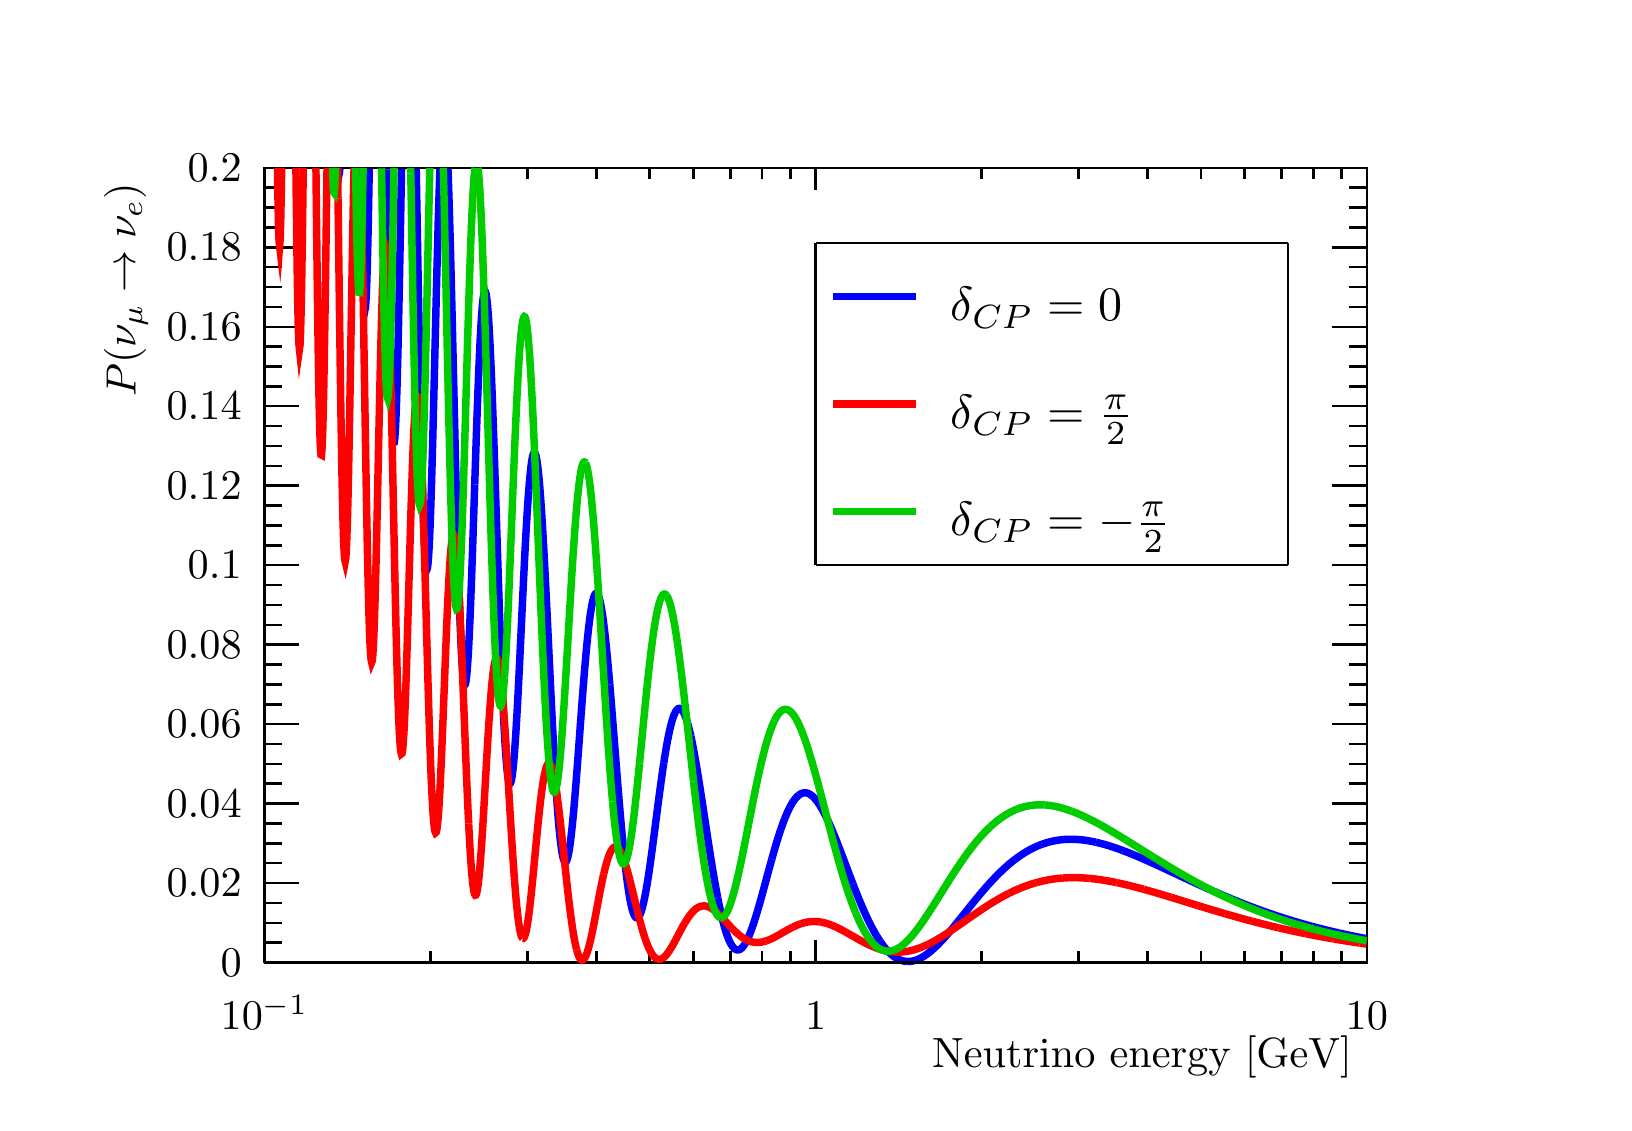
\begin{tikzpicture}
\pgfdeclareplotmark{cross} {
\pgfpathmoveto{\pgfpoint{-0.3\pgfplotmarksize}{\pgfplotmarksize}}
\pgfpathlineto{\pgfpoint{+0.3\pgfplotmarksize}{\pgfplotmarksize}}
\pgfpathlineto{\pgfpoint{+0.3\pgfplotmarksize}{0.3\pgfplotmarksize}}
\pgfpathlineto{\pgfpoint{+1\pgfplotmarksize}{0.3\pgfplotmarksize}}
\pgfpathlineto{\pgfpoint{+1\pgfplotmarksize}{-0.3\pgfplotmarksize}}
\pgfpathlineto{\pgfpoint{+0.3\pgfplotmarksize}{-0.3\pgfplotmarksize}}
\pgfpathlineto{\pgfpoint{+0.3\pgfplotmarksize}{-1.\pgfplotmarksize}}
\pgfpathlineto{\pgfpoint{-0.3\pgfplotmarksize}{-1.\pgfplotmarksize}}
\pgfpathlineto{\pgfpoint{-0.3\pgfplotmarksize}{-0.3\pgfplotmarksize}}
\pgfpathlineto{\pgfpoint{-1.\pgfplotmarksize}{-0.3\pgfplotmarksize}}
\pgfpathlineto{\pgfpoint{-1.\pgfplotmarksize}{0.3\pgfplotmarksize}}
\pgfpathlineto{\pgfpoint{-0.3\pgfplotmarksize}{0.3\pgfplotmarksize}}
\pgfpathclose
\pgfusepathqstroke
}
\pgfdeclareplotmark{cross*} {
\pgfpathmoveto{\pgfpoint{-0.3\pgfplotmarksize}{\pgfplotmarksize}}
\pgfpathlineto{\pgfpoint{+0.3\pgfplotmarksize}{\pgfplotmarksize}}
\pgfpathlineto{\pgfpoint{+0.3\pgfplotmarksize}{0.3\pgfplotmarksize}}
\pgfpathlineto{\pgfpoint{+1\pgfplotmarksize}{0.3\pgfplotmarksize}}
\pgfpathlineto{\pgfpoint{+1\pgfplotmarksize}{-0.3\pgfplotmarksize}}
\pgfpathlineto{\pgfpoint{+0.3\pgfplotmarksize}{-0.3\pgfplotmarksize}}
\pgfpathlineto{\pgfpoint{+0.3\pgfplotmarksize}{-1.\pgfplotmarksize}}
\pgfpathlineto{\pgfpoint{-0.3\pgfplotmarksize}{-1.\pgfplotmarksize}}
\pgfpathlineto{\pgfpoint{-0.3\pgfplotmarksize}{-0.3\pgfplotmarksize}}
\pgfpathlineto{\pgfpoint{-1.\pgfplotmarksize}{-0.3\pgfplotmarksize}}
\pgfpathlineto{\pgfpoint{-1.\pgfplotmarksize}{0.3\pgfplotmarksize}}
\pgfpathlineto{\pgfpoint{-0.3\pgfplotmarksize}{0.3\pgfplotmarksize}}
\pgfpathclose
\pgfusepathqfillstroke
}
\pgfdeclareplotmark{newstar} {
\pgfpathmoveto{\pgfqpoint{0pt}{\pgfplotmarksize}}
\pgfpathlineto{\pgfqpointpolar{44}{0.5\pgfplotmarksize}}
\pgfpathlineto{\pgfqpointpolar{18}{\pgfplotmarksize}}
\pgfpathlineto{\pgfqpointpolar{-20}{0.5\pgfplotmarksize}}
\pgfpathlineto{\pgfqpointpolar{-54}{\pgfplotmarksize}}
\pgfpathlineto{\pgfqpointpolar{-90}{0.5\pgfplotmarksize}}
\pgfpathlineto{\pgfqpointpolar{234}{\pgfplotmarksize}}
\pgfpathlineto{\pgfqpointpolar{198}{0.5\pgfplotmarksize}}
\pgfpathlineto{\pgfqpointpolar{162}{\pgfplotmarksize}}
\pgfpathlineto{\pgfqpointpolar{134}{0.5\pgfplotmarksize}}
\pgfpathclose
\pgfusepathqstroke
}
\pgfdeclareplotmark{newstar*} {
\pgfpathmoveto{\pgfqpoint{0pt}{\pgfplotmarksize}}
\pgfpathlineto{\pgfqpointpolar{44}{0.5\pgfplotmarksize}}
\pgfpathlineto{\pgfqpointpolar{18}{\pgfplotmarksize}}
\pgfpathlineto{\pgfqpointpolar{-20}{0.5\pgfplotmarksize}}
\pgfpathlineto{\pgfqpointpolar{-54}{\pgfplotmarksize}}
\pgfpathlineto{\pgfqpointpolar{-90}{0.5\pgfplotmarksize}}
\pgfpathlineto{\pgfqpointpolar{234}{\pgfplotmarksize}}
\pgfpathlineto{\pgfqpointpolar{198}{0.5\pgfplotmarksize}}
\pgfpathlineto{\pgfqpointpolar{162}{\pgfplotmarksize}}
\pgfpathlineto{\pgfqpointpolar{134}{0.5\pgfplotmarksize}}
\pgfpathclose
\pgfusepathqfillstroke
}
\definecolor{c}{rgb}{1,1,1};
\draw [color=c, fill=c] (0,0) rectangle (20,13.639);
\draw [color=c, fill=c] (3,1.77307) rectangle (17,11.8659);
\definecolor{c}{rgb}{0,0,0};
\draw [c,line width=0.9] (3,1.77307) -- (3,11.8659) -- (17,11.8659) -- (17,1.77307) -- (3,1.77307);
\definecolor{c}{rgb}{1,1,1};
\draw [color=c, fill=c] (3,1.77307) rectangle (17,11.8659);
\definecolor{c}{rgb}{0,0,0};
\draw [c,line width=0.9] (3,1.77307) -- (3,11.8659) -- (17,11.8659) -- (17,1.77307) -- (3,1.77307);
\definecolor{c}{rgb}{0,0,1};
\draw [c,line width=2.7] (3.94049,11.8659) -- (3.9415,11.8444);
\draw [c,line width=2.7] (3.9415,11.8444) -- (3.9485,11.7886) -- (3.9555,11.8248) -- (3.95779,11.8659);
\draw [c,line width=2.7] (4.22591,11.8659) -- (4.2285,11.6911);
\draw [c,line width=2.7] (4.2285,11.6911) -- (4.2355,11.2708) -- (4.2425,10.9073) -- (4.2495,10.6053) -- (4.2565,10.3685) -- (4.2635,10.1994) -- (4.2705,10.0993) -- (4.2775,10.0685) -- (4.2845,10.1062) -- (4.2915,10.2102) -- (4.2985,10.3776) --
 (4.3055,10.6045) -- (4.3125,10.8858) -- (4.3195,11.2161) -- (4.3265,11.5889) -- (4.33125,11.8659);
\draw [c,line width=2.7] (4.55716,11.8659) -- (4.5575,11.8422);
\draw [c,line width=2.7] (4.5575,11.8422) -- (4.5645,11.3648) -- (4.5715,10.9074) -- (4.5785,10.4755) -- (4.5855,10.0739) -- (4.5925,9.70726) -- (4.5995,9.37944) -- (4.6065,9.09385) -- (4.6135,8.85328) -- (4.6205,8.6599) -- (4.6275,8.51523) --
 (4.6345,8.42015) -- (4.6415,8.37486) -- (4.6485,8.37897) -- (4.6555,8.43144) -- (4.6625,8.53063) -- (4.6695,8.67435) -- (4.6765,8.85988) -- (4.6835,9.08402) -- (4.6905,9.34314) -- (4.6975,9.63323) -- (4.7045,9.94997) -- (4.7115,10.2888) --
 (4.7185,10.6448) -- (4.7255,11.0132) -- (4.7325,11.3889) -- (4.7395,11.767) -- (4.74135,11.8659);
\draw [c,line width=2.7] (4.92712,11.8659) -- (4.9285,11.7895);
\draw [c,line width=2.7] (4.9285,11.7895) -- (4.9355,11.396) -- (4.9425,10.9983) -- (4.9495,10.6005) -- (4.9565,10.2062) -- (4.9635,9.8192) -- (4.9705,9.44312) -- (4.9775,9.08136) -- (4.9845,8.73713) -- (4.9915,8.41344) -- (4.9985,8.11302) --
 (5.0055,7.83835) -- (5.0125,7.59159) -- (5.0195,7.3746) -- (5.0265,7.18891) -- (5.0335,7.03572) -- (5.0405,6.9159) -- (5.0475,6.82996) -- (5.0545,6.77808) -- (5.0615,6.76011) -- (5.0685,6.77555) -- (5.0755,6.82362) -- (5.0825,6.90321) --
 (5.0895,7.01293) -- (5.0965,7.15114) -- (5.1035,7.31594) -- (5.1105,7.5052) -- (5.1175,7.71661) -- (5.1245,7.94768) -- (5.1315,8.19577) -- (5.1385,8.45814) -- (5.1455,8.73193) -- (5.1525,9.01425) -- (5.1595,9.30215) -- (5.1665,9.59269) --
 (5.1735,9.88295) -- (5.1805,10.1701) -- (5.1875,10.4512) -- (5.1945,10.7237) -- (5.2015,10.9849) -- (5.2085,11.2325) -- (5.2155,11.4641) -- (5.2225,11.6775) -- (5.22932,11.8659);
\draw [c,line width=2.7] (5.33001,11.8659) -- (5.3345,11.7474);
\draw [c,line width=2.7] (5.3345,11.7474) -- (5.3415,11.5422) -- (5.3485,11.3182) -- (5.3555,11.0772) -- (5.3625,10.8212) -- (5.3695,10.5521) -- (5.3765,10.2719) -- (5.3835,9.98293) -- (5.3905,9.68718) -- (5.3975,9.38688) -- (5.4045,9.08421) --
 (5.4115,8.78134) -- (5.4185,8.48042) -- (5.4255,8.18354) -- (5.4325,7.89274) -- (5.4395,7.60996) -- (5.4465,7.33707) -- (5.4535,7.07583) -- (5.4605,6.8279) -- (5.4675,6.5948) -- (5.4745,6.37792) -- (5.4815,6.1785) -- (5.4885,5.99765) --
 (5.4955,5.83631) -- (5.5025,5.69528) -- (5.5095,5.57519) -- (5.5165,5.4765) -- (5.5235,5.39952) -- (5.5305,5.3444) -- (5.5375,5.31112) -- (5.5445,5.29952) -- (5.5515,5.30927) -- (5.5585,5.33991) -- (5.5655,5.39084) -- (5.5725,5.4613) --
 (5.5795,5.55045) -- (5.5865,5.65729) -- (5.5935,5.78074) -- (5.6005,5.91961) -- (5.6075,6.07264) -- (5.6145,6.23846) -- (5.6215,6.41566) -- (5.6285,6.60277) -- (5.6355,6.79827) -- (5.6425,7.00062) -- (5.6495,7.20824) -- (5.6565,7.41955) --
 (5.6635,7.63296) -- (5.6705,7.84692);
\draw [c,line width=2.7] (5.6705,7.84692) -- (5.6775,8.05986) -- (5.6845,8.27027) -- (5.6915,8.47667) -- (5.6985,8.67762) -- (5.7055,8.87176) -- (5.7125,9.05777) -- (5.7195,9.23442) -- (5.7265,9.40055) -- (5.7335,9.5551) -- (5.7405,9.69707) --
 (5.7475,9.82559) -- (5.7545,9.93986) -- (5.7615,10.0392) -- (5.7685,10.123) -- (5.7755,10.1908) -- (5.7825,10.2423) -- (5.7895,10.2771) -- (5.7965,10.2951) -- (5.8035,10.2962) -- (5.8105,10.2805) -- (5.8175,10.2482) -- (5.8245,10.1995) --
 (5.8315,10.1347) -- (5.8385,10.0542) -- (5.8455,9.95864) -- (5.8525,9.84855) -- (5.8595,9.7246) -- (5.8665,9.58755) -- (5.8735,9.43822) -- (5.8805,9.27746) -- (5.8875,9.10621) -- (5.8945,8.92544) -- (5.9015,8.73615) -- (5.9085,8.5394) --
 (5.9155,8.33624) -- (5.9225,8.12778) -- (5.9295,7.91512) -- (5.9365,7.69936) -- (5.9435,7.48163) -- (5.9505,7.26303) -- (5.9575,7.04465) -- (5.9645,6.82757) -- (5.9715,6.61285) -- (5.9785,6.40152) -- (5.9855,6.19456) -- (5.9925,5.99294) --
 (5.9995,5.79756) -- (6.0065,5.60929) -- (6.0135,5.42895);
\draw [c,line width=2.7] (6.0135,5.42895) -- (6.0205,5.25729) -- (6.0275,5.09503) -- (6.0345,4.94281) -- (6.0415,4.80121) -- (6.0485,4.67075) -- (6.0555,4.55189) -- (6.0625,4.44501) -- (6.0695,4.35044) -- (6.0765,4.26843) -- (6.0835,4.19918) --
 (6.0905,4.14279) -- (6.0975,4.09933) -- (6.1045,4.06878) -- (6.1115,4.05107) -- (6.1185,4.04607) -- (6.1255,4.05357) -- (6.1325,4.07332) -- (6.1395,4.105) -- (6.1465,4.14827) -- (6.1535,4.20269) -- (6.1605,4.26781) -- (6.1675,4.34312) --
 (6.1745,4.42808) -- (6.1815,4.5221) -- (6.1885,4.62456) -- (6.1955,4.73481) -- (6.2025,4.85218) -- (6.2095,4.97598) -- (6.2165,5.10547) -- (6.2235,5.23994) -- (6.2305,5.37864) -- (6.2375,5.52082) -- (6.2445,5.66571) -- (6.2515,5.81257) --
 (6.2585,5.96064) -- (6.2655,6.10918) -- (6.2725,6.25743) -- (6.2795,6.40469) -- (6.2865,6.55023) -- (6.2935,6.69338) -- (6.3005,6.83345) -- (6.3075,6.9698) -- (6.3145,7.10181) -- (6.3215,7.2289) -- (6.3285,7.3505) -- (6.3355,7.46608) --
 (6.3425,7.57514) -- (6.3495,7.67724) -- (6.3565,7.77195);
\draw [c,line width=2.7] (6.3565,7.77195) -- (6.3635,7.85888) -- (6.3705,7.9377) -- (6.3775,8.00809) -- (6.3845,8.06979) -- (6.3915,8.12258) -- (6.3985,8.16628) -- (6.4055,8.20073) -- (6.4125,8.22585) -- (6.4195,8.24156) -- (6.4265,8.24784) --
 (6.4335,8.24471) -- (6.4405,8.23222) -- (6.4475,8.21047) -- (6.4545,8.17958) -- (6.4615,8.13972) -- (6.4685,8.09107) -- (6.4755,8.03387) -- (6.4825,7.96837) -- (6.4895,7.89487) -- (6.4965,7.81367) -- (6.5035,7.72511) -- (6.5105,7.62956) --
 (6.5175,7.52741) -- (6.5245,7.41905) -- (6.5315,7.3049) -- (6.5385,7.18542) -- (6.5455,7.06104) -- (6.5525,6.93224) -- (6.5595,6.79948) -- (6.5665,6.66325) -- (6.5735,6.52403) -- (6.5805,6.38232) -- (6.5875,6.23861) -- (6.5945,6.09339) --
 (6.6015,5.94716) -- (6.6085,5.8004) -- (6.6155,5.65359) -- (6.6225,5.50722) -- (6.6295,5.36174) -- (6.6365,5.21762) -- (6.6435,5.07531) -- (6.6505,4.93523) -- (6.6575,4.7978) -- (6.6645,4.66344) -- (6.6715,4.53252) -- (6.6785,4.40541) --
 (6.6855,4.28248) -- (6.6925,4.16403) -- (6.6995,4.0504);
\draw [c,line width=2.7] (6.6995,4.0504) -- (6.7065,3.94186) -- (6.7135,3.8387) -- (6.7205,3.74114) -- (6.7275,3.64942) -- (6.7345,3.56375) -- (6.7415,3.48429) -- (6.7485,3.4112) -- (6.7555,3.34462) -- (6.7625,3.28465) -- (6.7695,3.23138) --
 (6.7765,3.18487) -- (6.7835,3.14517) -- (6.7905,3.11228) -- (6.7975,3.0862) -- (6.8045,3.06691) -- (6.8115,3.05436) -- (6.8185,3.04848) -- (6.8255,3.04918) -- (6.8325,3.05635) -- (6.8395,3.06987) -- (6.8465,3.0896) -- (6.8535,3.11537) --
 (6.8605,3.147) -- (6.8675,3.18431) -- (6.8745,3.22708) -- (6.8815,3.2751) -- (6.8885,3.32813) -- (6.8955,3.38593) -- (6.9025,3.44824) -- (6.9095,3.5148) -- (6.9165,3.58533) -- (6.9235,3.65956) -- (6.9305,3.73718) -- (6.9375,3.81792) --
 (6.9445,3.90148) -- (6.9515,3.98754) -- (6.9585,4.07582) -- (6.9655,4.16599) -- (6.9725,4.25776) -- (6.9795,4.35081) -- (6.9865,4.44485) -- (6.9935,4.53956) -- (7.0005,4.63465) -- (7.0075,4.72981) -- (7.0145,4.82477) -- (7.0215,4.91921) --
 (7.0285,5.01288) -- (7.0355,5.10548) -- (7.0425,5.19675);
\draw [c,line width=2.7] (7.0425,5.19675) -- (7.0495,5.28643) -- (7.0565,5.37426) -- (7.0635,5.46001) -- (7.0705,5.54344) -- (7.0775,5.62431) -- (7.0845,5.70243) -- (7.0915,5.77759) -- (7.0985,5.84958) -- (7.1055,5.91824) -- (7.1125,5.9834) --
 (7.1195,6.04489) -- (7.1265,6.10257) -- (7.1335,6.1563) -- (7.1405,6.20598) -- (7.1475,6.25148) -- (7.1545,6.29271) -- (7.1615,6.3296) -- (7.1685,6.36206) -- (7.1755,6.39004) -- (7.1825,6.41349) -- (7.1895,6.43238) -- (7.1965,6.44669) --
 (7.2035,6.45641) -- (7.2105,6.46153) -- (7.2175,6.46208) -- (7.2245,6.45807) -- (7.2315,6.44954) -- (7.2385,6.43654) -- (7.2455,6.41913) -- (7.2525,6.39737) -- (7.2595,6.37133) -- (7.2665,6.3411) -- (7.2735,6.30678) -- (7.2805,6.26846) --
 (7.2875,6.22626) -- (7.2945,6.1803) -- (7.3015,6.1307) -- (7.3085,6.07759) -- (7.3155,6.02111) -- (7.3225,5.96141) -- (7.3295,5.89864) -- (7.3365,5.83294) -- (7.3435,5.76449) -- (7.3505,5.69344) -- (7.3575,5.61995) -- (7.3645,5.54421) --
 (7.3715,5.46638) -- (7.3785,5.38664) -- (7.3855,5.30516);
\draw [c,line width=2.7] (7.3855,5.30516) -- (7.3925,5.22212) -- (7.3995,5.1377) -- (7.4065,5.05208) -- (7.4135,4.96544) -- (7.4205,4.87796) -- (7.4275,4.78981) -- (7.4345,4.70118) -- (7.4415,4.61224) -- (7.4485,4.52316) -- (7.4555,4.43412) --
 (7.4625,4.34528) -- (7.4695,4.25681) -- (7.4765,4.16888) -- (7.4835,4.08164) -- (7.4905,3.99525) -- (7.4975,3.90986) -- (7.5045,3.82562) -- (7.5115,3.74267) -- (7.5185,3.66116) -- (7.5255,3.58121) -- (7.5325,3.50295) -- (7.5395,3.42651) --
 (7.5465,3.35201) -- (7.5535,3.27955) -- (7.5605,3.20925) -- (7.5675,3.14121) -- (7.5745,3.07551) -- (7.5815,3.01225) -- (7.5885,2.95152) -- (7.5955,2.89338) -- (7.6025,2.83792) -- (7.6095,2.78519) -- (7.6165,2.73525) -- (7.6235,2.68815) --
 (7.6305,2.64395) -- (7.6375,2.60268) -- (7.6445,2.56437) -- (7.6515,2.52906) -- (7.6585,2.49676) -- (7.6655,2.46749) -- (7.6725,2.44126) -- (7.6795,2.41808) -- (7.6865,2.39794) -- (7.6935,2.38083) -- (7.7005,2.36675) -- (7.7075,2.35567) --
 (7.7145,2.34758) -- (7.7215,2.34244) -- (7.7285,2.34023);
\draw [c,line width=2.7] (7.7285,2.34023) -- (7.7355,2.34089) -- (7.7425,2.34441) -- (7.7495,2.35071) -- (7.7565,2.35977) -- (7.7635,2.37151) -- (7.7705,2.38589) -- (7.7775,2.40283) -- (7.7845,2.42228) -- (7.7915,2.44416) -- (7.7985,2.46841) --
 (7.8055,2.49494) -- (7.8125,2.52368) -- (7.8195,2.55455) -- (7.8265,2.58746) -- (7.8335,2.62233) -- (7.8405,2.65907) -- (7.8475,2.69759) -- (7.8545,2.73781) -- (7.8615,2.77962) -- (7.8685,2.82294) -- (7.8755,2.86766) -- (7.8825,2.91371) --
 (7.8895,2.96097) -- (7.8965,3.00935) -- (7.9035,3.05876) -- (7.9105,3.10909) -- (7.9175,3.16025) -- (7.9245,3.21214) -- (7.9315,3.26467) -- (7.9385,3.31773) -- (7.9455,3.37124) -- (7.9525,3.42509) -- (7.9595,3.4792) -- (7.9665,3.53346) --
 (7.9735,3.58779) -- (7.9805,3.64209) -- (7.9875,3.69628) -- (7.9945,3.75026) -- (8.0015,3.80395) -- (8.0085,3.85727) -- (8.0155,3.91013) -- (8.0225,3.96246) -- (8.0295,4.01416) -- (8.0365,4.06517) -- (8.0435,4.11541) -- (8.0505,4.1648) --
 (8.0575,4.21329) -- (8.0645,4.26079) -- (8.0715,4.30724);
\draw [c,line width=2.7] (8.0715,4.30724) -- (8.0785,4.35259) -- (8.0855,4.39677) -- (8.0925,4.43972) -- (8.0995,4.48138) -- (8.1065,4.52172) -- (8.1135,4.56066) -- (8.1205,4.59818) -- (8.1275,4.63422) -- (8.1345,4.66874) -- (8.1415,4.7017) --
 (8.1485,4.73307) -- (8.1555,4.76282) -- (8.1625,4.79091) -- (8.1695,4.81731) -- (8.1765,4.842) -- (8.1835,4.86497) -- (8.1905,4.88618) -- (8.1975,4.90562) -- (8.2045,4.92327) -- (8.2115,4.93914) -- (8.2185,4.9532) -- (8.2255,4.96544) --
 (8.2325,4.97588) -- (8.2395,4.9845) -- (8.2465,4.9913) -- (8.2535,4.99629) -- (8.2605,4.99948) -- (8.2675,5.00087) -- (8.2745,5.00047) -- (8.2815,4.99829) -- (8.2885,4.99436) -- (8.2955,4.98868) -- (8.3025,4.98128) -- (8.3095,4.97217) --
 (8.3165,4.96137) -- (8.3235,4.94892) -- (8.3305,4.93484) -- (8.3375,4.91915) -- (8.3445,4.90189) -- (8.3515,4.88308) -- (8.3585,4.86276) -- (8.3655,4.84097) -- (8.3725,4.81773) -- (8.3795,4.79308) -- (8.3865,4.76706) -- (8.3935,4.73972) --
 (8.4005,4.71108) -- (8.4075,4.68119) -- (8.4145,4.6501);
\draw [c,line width=2.7] (8.4145,4.6501) -- (8.4215,4.61784) -- (8.4285,4.58446) -- (8.4355,4.55) -- (8.4425,4.51451) -- (8.4495,4.47803) -- (8.4565,4.44061) -- (8.4635,4.4023) -- (8.4705,4.36313) -- (8.4775,4.32317) -- (8.4845,4.28245) --
 (8.4915,4.24103) -- (8.4985,4.19895) -- (8.5055,4.15625) -- (8.5125,4.113) -- (8.5195,4.06923) -- (8.5265,4.02499) -- (8.5335,3.98033) -- (8.5405,3.9353) -- (8.5475,3.88995) -- (8.5545,3.84432) -- (8.5615,3.79846) -- (8.5685,3.75241) --
 (8.5755,3.70623) -- (8.5825,3.65994) -- (8.5895,3.61362) -- (8.5965,3.56728) -- (8.6035,3.52099) -- (8.6105,3.47477) -- (8.6175,3.42868) -- (8.6245,3.38276) -- (8.6315,3.33704) -- (8.6385,3.29157) -- (8.6455,3.24638) -- (8.6525,3.20152) --
 (8.6595,3.15703) -- (8.6665,3.11293) -- (8.6735,3.06926) -- (8.6805,3.02607) -- (8.6875,2.98338) -- (8.6945,2.94122) -- (8.7015,2.89964) -- (8.7085,2.85865) -- (8.7155,2.81829) -- (8.7225,2.7786) -- (8.7295,2.73959) -- (8.7365,2.70129) --
 (8.7435,2.66373) -- (8.7505,2.62694) -- (8.7575,2.59093);
\draw [c,line width=2.7] (8.7575,2.59093) -- (8.7645,2.55574) -- (8.7715,2.52138) -- (8.7785,2.48787) -- (8.7855,2.45524) -- (8.7925,2.42349) -- (8.7995,2.39266) -- (8.8065,2.36274) -- (8.8135,2.33377) -- (8.8205,2.30575) -- (8.8275,2.2787) --
 (8.8345,2.25262) -- (8.8415,2.22754) -- (8.8485,2.20345) -- (8.8555,2.18037) -- (8.8625,2.1583) -- (8.8695,2.13726) -- (8.8765,2.11725) -- (8.8835,2.09827) -- (8.8905,2.08032) -- (8.8975,2.06342) -- (8.9045,2.04756) -- (8.9115,2.03273) --
 (8.9185,2.01896) -- (8.9255,2.00622) -- (8.9325,1.99452) -- (8.9395,1.98386) -- (8.9465,1.97423) -- (8.9535,1.96563) -- (8.9605,1.95806) -- (8.9675,1.9515) -- (8.9745,1.94596) -- (8.9815,1.94142) -- (8.9885,1.93787) -- (8.9955,1.93531) --
 (9.0025,1.93373) -- (9.0095,1.93312) -- (9.0165,1.93346) -- (9.0235,1.93475) -- (9.0305,1.93697) -- (9.0375,1.94011) -- (9.0445,1.94416) -- (9.0515,1.9491) -- (9.0585,1.95492) -- (9.0655,1.9616) -- (9.0725,1.96913) -- (9.0795,1.97749) --
 (9.0865,1.98667) -- (9.0935,1.99665) -- (9.1005,2.00741);
\draw [c,line width=2.7] (9.1005,2.00741) -- (9.1075,2.01893) -- (9.1145,2.03121) -- (9.1215,2.04421) -- (9.1285,2.05792) -- (9.1355,2.07233) -- (9.1425,2.08741) -- (9.1495,2.10314) -- (9.1565,2.11951) -- (9.1635,2.13649) -- (9.1705,2.15407) --
 (9.1775,2.17222) -- (9.1845,2.19092) -- (9.1915,2.21017) -- (9.1985,2.22992) -- (9.2055,2.25017) -- (9.2125,2.27089) -- (9.2195,2.29206) -- (9.2265,2.31367) -- (9.2335,2.33569) -- (9.2405,2.35809) -- (9.2475,2.38087) -- (9.2545,2.40399) --
 (9.2615,2.42745) -- (9.2685,2.45121) -- (9.2755,2.47526) -- (9.2825,2.49957) -- (9.2895,2.52413) -- (9.2965,2.54892) -- (9.3035,2.57391) -- (9.3105,2.59908) -- (9.3175,2.62443) -- (9.3245,2.64992) -- (9.3315,2.67553) -- (9.3385,2.70125) --
 (9.3455,2.72707) -- (9.3525,2.75295) -- (9.3595,2.77888) -- (9.3665,2.80484) -- (9.3735,2.83081) -- (9.3805,2.85679) -- (9.3875,2.88274) -- (9.3945,2.90865) -- (9.4015,2.9345) -- (9.4085,2.96028) -- (9.4155,2.98597) -- (9.4225,3.01155) --
 (9.4295,3.03701) -- (9.4365,3.06232) -- (9.4435,3.08749);
\draw [c,line width=2.7] (9.4435,3.08749) -- (9.4505,3.11248) -- (9.4575,3.13729) -- (9.4645,3.16191) -- (9.4715,3.1863) -- (9.4785,3.21048) -- (9.4855,3.23441) -- (9.4925,3.25808) -- (9.4995,3.28149) -- (9.5065,3.30462) -- (9.5135,3.32746) --
 (9.5205,3.34999) -- (9.5275,3.37221) -- (9.5345,3.39411) -- (9.5415,3.41566) -- (9.5485,3.43687) -- (9.5555,3.45772) -- (9.5625,3.47821) -- (9.5695,3.49832) -- (9.5765,3.51804) -- (9.5835,3.53737) -- (9.5905,3.55629) -- (9.5975,3.57481) --
 (9.6045,3.59291) -- (9.6115,3.61058) -- (9.6185,3.62782) -- (9.6255,3.64461) -- (9.6325,3.66097) -- (9.6395,3.67687) -- (9.6465,3.69232) -- (9.6535,3.7073) -- (9.6605,3.72182) -- (9.6675,3.73587) -- (9.6745,3.74944) -- (9.6815,3.76253) --
 (9.6885,3.77514) -- (9.6955,3.78727) -- (9.7025,3.7989) -- (9.7095,3.81004) -- (9.7165,3.82069) -- (9.7235,3.83084) -- (9.7305,3.8405) -- (9.7375,3.84965) -- (9.7445,3.85831) -- (9.7515,3.86646) -- (9.7585,3.87411) -- (9.7655,3.88127) --
 (9.7725,3.88791) -- (9.7795,3.89406) -- (9.7865,3.89971);
\draw [c,line width=2.7] (9.7865,3.89971) -- (9.7935,3.90485) -- (9.8005,3.9095) -- (9.8075,3.91365) -- (9.8145,3.9173) -- (9.8215,3.92046) -- (9.8285,3.92313) -- (9.8355,3.92531) -- (9.8425,3.92699) -- (9.8495,3.9282) -- (9.8565,3.92892) --
 (9.8635,3.92916) -- (9.8705,3.92893) -- (9.8775,3.92822) -- (9.8845,3.92705) -- (9.8915,3.92541) -- (9.8985,3.92332) -- (9.9055,3.92076) -- (9.9125,3.91776) -- (9.9195,3.9143) -- (9.9265,3.91041) -- (9.9335,3.90608) -- (9.9405,3.90131) --
 (9.9475,3.89612) -- (9.9545,3.89051) -- (9.9615,3.88448) -- (9.9685,3.87804) -- (9.9755,3.8712) -- (9.9825,3.86396) -- (9.9895,3.85632) -- (9.9965,3.8483) -- (10.0035,3.83989) -- (10.0105,3.83112) -- (10.0175,3.82197) -- (10.0245,3.81246) --
 (10.0315,3.8026) -- (10.0385,3.79239) -- (10.0455,3.78184) -- (10.0525,3.77095) -- (10.0595,3.75974) -- (10.0665,3.7482) -- (10.0735,3.73636) -- (10.0805,3.7242) -- (10.0875,3.71174) -- (10.0945,3.69899) -- (10.1015,3.68596) -- (10.1085,3.67265) --
 (10.1155,3.65906) -- (10.1225,3.64521) -- (10.1295,3.63111);
\draw [c,line width=2.7] (10.1295,3.63111) -- (10.1365,3.61676) -- (10.1435,3.60216) -- (10.1505,3.58733) -- (10.1575,3.57227) -- (10.1645,3.55699) -- (10.1715,3.5415) -- (10.1785,3.52581) -- (10.1855,3.50991) -- (10.1925,3.49383) --
 (10.1995,3.47756) -- (10.2065,3.46111) -- (10.2135,3.4445) -- (10.2205,3.42772) -- (10.2275,3.41079) -- (10.2345,3.39372) -- (10.2415,3.3765) -- (10.2485,3.35915) -- (10.2555,3.34168) -- (10.2625,3.32408) -- (10.2695,3.30638) -- (10.2765,3.28857) --
 (10.2835,3.27066) -- (10.2905,3.25266) -- (10.2975,3.23458) -- (10.3045,3.21642) -- (10.3115,3.19819) -- (10.3185,3.1799) -- (10.3255,3.16155) -- (10.3325,3.14315) -- (10.3395,3.1247) -- (10.3465,3.10622) -- (10.3535,3.08771) -- (10.3605,3.06917) --
 (10.3675,3.05061) -- (10.3745,3.03204) -- (10.3815,3.01346) -- (10.3885,2.99489) -- (10.3955,2.97632) -- (10.4025,2.95776) -- (10.4095,2.93921) -- (10.4165,2.92069) -- (10.4235,2.9022) -- (10.4305,2.88375) -- (10.4375,2.86533) -- (10.4445,2.84696)
 -- (10.4515,2.82863) -- (10.4585,2.81037) -- (10.4655,2.79216) -- (10.4725,2.77402);
\draw [c,line width=2.7] (10.4725,2.77402) -- (10.4795,2.75595) -- (10.4865,2.73796) -- (10.4935,2.72005) -- (10.5005,2.70222) -- (10.5075,2.68448) -- (10.5145,2.66684) -- (10.5215,2.64929) -- (10.5285,2.63185) -- (10.5355,2.61451) --
 (10.5425,2.59729) -- (10.5495,2.58018) -- (10.5565,2.5632) -- (10.5635,2.54633) -- (10.5705,2.5296) -- (10.5775,2.51299) -- (10.5845,2.49652) -- (10.5915,2.48019) -- (10.5985,2.464) -- (10.6055,2.44795) -- (10.6125,2.43206) -- (10.6195,2.41631) --
 (10.6265,2.40072) -- (10.6335,2.38529) -- (10.6405,2.37002) -- (10.6475,2.35491) -- (10.6545,2.33997) -- (10.6615,2.3252) -- (10.6685,2.3106) -- (10.6755,2.29617) -- (10.6825,2.28192) -- (10.6895,2.26785) -- (10.6965,2.25397) -- (10.7035,2.24026) --
 (10.7105,2.22674) -- (10.7175,2.21341) -- (10.7245,2.20027) -- (10.7315,2.18731) -- (10.7385,2.17456) -- (10.7455,2.16199) -- (10.7525,2.14963) -- (10.7595,2.13746) -- (10.7665,2.12549) -- (10.7735,2.11372) -- (10.7805,2.10215) -- (10.7875,2.09079)
 -- (10.7945,2.07963) -- (10.8015,2.06867) -- (10.8085,2.05793) -- (10.8155,2.04738);
\draw [c,line width=2.7] (10.8155,2.04738) -- (10.8225,2.03705) -- (10.8295,2.02693) -- (10.8365,2.01702) -- (10.8435,2.00731) -- (10.8505,1.99782) -- (10.8575,1.98854) -- (10.8645,1.97947) -- (10.8715,1.97062) -- (10.8785,1.96197) --
 (10.8855,1.95354) -- (10.8925,1.94532) -- (10.8995,1.93732) -- (10.9065,1.92953) -- (10.9135,1.92195) -- (10.9205,1.91458) -- (10.9275,1.90743) -- (10.9345,1.90049) -- (10.9415,1.89377) -- (10.9485,1.88725) -- (10.9555,1.88095) -- (10.9625,1.87486)
 -- (10.9695,1.86898) -- (10.9765,1.86332) -- (10.9835,1.85786) -- (10.9905,1.85261) -- (10.9975,1.84757) -- (11.0045,1.84274) -- (11.0115,1.83812) -- (11.0185,1.8337) -- (11.0255,1.8295) -- (11.0325,1.82549) -- (11.0395,1.82169) -- (11.0465,1.81809)
 -- (11.0535,1.8147) -- (11.0605,1.81151) -- (11.0675,1.80852) -- (11.0745,1.80572) -- (11.0815,1.80313) -- (11.0885,1.80073) -- (11.0955,1.79853) -- (11.1025,1.79652) -- (11.1095,1.79471) -- (11.1165,1.79309) -- (11.1235,1.79166) --
 (11.1305,1.79041) -- (11.1375,1.78936) -- (11.1445,1.78849) -- (11.1515,1.78781) -- (11.1585,1.78731);
\draw [c,line width=2.7] (11.1585,1.78731) -- (11.1655,1.787) -- (11.1725,1.78686) -- (11.1795,1.7869) -- (11.1865,1.78712) -- (11.1935,1.78752) -- (11.2005,1.78809) -- (11.2075,1.78883) -- (11.2145,1.78974) -- (11.2215,1.79083) -- (11.2285,1.79208)
 -- (11.2355,1.79349) -- (11.2425,1.79508) -- (11.2495,1.79682) -- (11.2565,1.79872) -- (11.2635,1.80078) -- (11.2705,1.803) -- (11.2775,1.80538) -- (11.2845,1.8079) -- (11.2915,1.81058) -- (11.2985,1.81341) -- (11.3055,1.81639) -- (11.3125,1.81951)
 -- (11.3195,1.82278) -- (11.3265,1.82619) -- (11.3335,1.82974) -- (11.3405,1.83342) -- (11.3475,1.83725) -- (11.3545,1.84121) -- (11.3615,1.8453) -- (11.3685,1.84952) -- (11.3755,1.85387) -- (11.3825,1.85835) -- (11.3895,1.86295) --
 (11.3965,1.86768) -- (11.4035,1.87252) -- (11.4105,1.87749) -- (11.4175,1.88257) -- (11.4245,1.88777) -- (11.4315,1.89308) -- (11.4385,1.8985) -- (11.4455,1.90403) -- (11.4525,1.90967) -- (11.4595,1.91542) -- (11.4665,1.92126) -- (11.4735,1.92721)
 -- (11.4805,1.93326) -- (11.4875,1.93941) -- (11.4945,1.94565) -- (11.5015,1.95199);
\draw [c,line width=2.7] (11.5015,1.95199) -- (11.5085,1.95842) -- (11.5155,1.96493) -- (11.5225,1.97154) -- (11.5295,1.97823) -- (11.5365,1.98501) -- (11.5435,1.99187) -- (11.5505,1.99881) -- (11.5575,2.00582) -- (11.5645,2.01292) --
 (11.5715,2.02009) -- (11.5785,2.02733) -- (11.5855,2.03464) -- (11.5925,2.04202) -- (11.5995,2.04947) -- (11.6065,2.05699) -- (11.6135,2.06457) -- (11.6205,2.07221) -- (11.6275,2.07991) -- (11.6345,2.08767) -- (11.6415,2.09549) -- (11.6485,2.10336)
 -- (11.6555,2.11128) -- (11.6625,2.11926) -- (11.6695,2.12728) -- (11.6765,2.13535) -- (11.6835,2.14347) -- (11.6905,2.15164) -- (11.6975,2.15984) -- (11.7045,2.16809) -- (11.7115,2.17638) -- (11.7185,2.1847) -- (11.7255,2.19306) --
 (11.7325,2.20146) -- (11.7395,2.20989) -- (11.7465,2.21835) -- (11.7535,2.22684) -- (11.7605,2.23536) -- (11.7675,2.2439) -- (11.7745,2.25247) -- (11.7815,2.26106) -- (11.7885,2.26968) -- (11.7955,2.27831) -- (11.8025,2.28697) -- (11.8095,2.29564)
 -- (11.8165,2.30433) -- (11.8235,2.31304) -- (11.8305,2.32175) -- (11.8375,2.33048) -- (11.8445,2.33922);
\draw [c,line width=2.7] (11.8445,2.33922) -- (11.8515,2.34797) -- (11.8585,2.35673) -- (11.8655,2.36549) -- (11.8725,2.37426) -- (11.8795,2.38303) -- (11.8865,2.3918) -- (11.8935,2.40058) -- (11.9005,2.40935) -- (11.9075,2.41813) -- (11.9145,2.4269)
 -- (11.9215,2.43567) -- (11.9285,2.44443) -- (11.9355,2.45319) -- (11.9425,2.46194) -- (11.9495,2.47068) -- (11.9565,2.47941) -- (11.9635,2.48813) -- (11.9705,2.49684) -- (11.9775,2.50553) -- (11.9845,2.51421) -- (11.9915,2.52288) --
 (11.9985,2.53153) -- (12.0055,2.54016) -- (12.0125,2.54877) -- (12.0195,2.55737) -- (12.0265,2.56594) -- (12.0335,2.57449) -- (12.0405,2.58302) -- (12.0475,2.59153) -- (12.0545,2.60001) -- (12.0615,2.60847) -- (12.0685,2.6169) -- (12.0755,2.62531)
 -- (12.0825,2.63368) -- (12.0895,2.64203) -- (12.0965,2.65035) -- (12.1035,2.65864) -- (12.1105,2.6669) -- (12.1175,2.67512) -- (12.1245,2.68331) -- (12.1315,2.69147) -- (12.1385,2.69959) -- (12.1455,2.70768) -- (12.1525,2.71574) --
 (12.1595,2.72375) -- (12.1665,2.73173) -- (12.1735,2.73967) -- (12.1805,2.74758) -- (12.1875,2.75544);
\draw [c,line width=2.7] (12.1875,2.75544) -- (12.1945,2.76326) -- (12.2015,2.77104) -- (12.2085,2.77879) -- (12.2155,2.78649) -- (12.2225,2.79414) -- (12.2295,2.80176) -- (12.2365,2.80933) -- (12.2435,2.81685) -- (12.2505,2.82433) --
 (12.2575,2.83177) -- (12.2645,2.83916) -- (12.2715,2.84651) -- (12.2785,2.8538) -- (12.2855,2.86105) -- (12.2925,2.86826) -- (12.2995,2.87541) -- (12.3065,2.88252) -- (12.3135,2.88957) -- (12.3205,2.89658) -- (12.3275,2.90354) -- (12.3345,2.91044)
 -- (12.3415,2.9173) -- (12.3485,2.9241) -- (12.3555,2.93086) -- (12.3625,2.93756) -- (12.3695,2.94421) -- (12.3765,2.9508) -- (12.3835,2.95735) -- (12.3905,2.96384) -- (12.3975,2.97028) -- (12.4045,2.97666) -- (12.4115,2.98299) -- (12.4185,2.98926)
 -- (12.4255,2.99548) -- (12.4325,3.00165) -- (12.4395,3.00776) -- (12.4465,3.01382) -- (12.4535,3.01982) -- (12.4605,3.02576) -- (12.4675,3.03165) -- (12.4745,3.03748) -- (12.4815,3.04326) -- (12.4885,3.04898) -- (12.4955,3.05464) --
 (12.5025,3.06025) -- (12.5095,3.0658) -- (12.5165,3.07129) -- (12.5235,3.07672) -- (12.5305,3.0821);
\draw [c,line width=2.7] (12.5305,3.0821) -- (12.5375,3.08742) -- (12.5445,3.09268) -- (12.5515,3.09789) -- (12.5585,3.10304) -- (12.5655,3.10813) -- (12.5725,3.11316) -- (12.5795,3.11813) -- (12.5865,3.12305) -- (12.5935,3.12791) --
 (12.6005,3.13271) -- (12.6075,3.13745) -- (12.6145,3.14213) -- (12.6215,3.14676) -- (12.6285,3.15132) -- (12.6355,3.15583) -- (12.6425,3.16028) -- (12.6495,3.16468) -- (12.6565,3.16901) -- (12.6635,3.17329) -- (12.6705,3.17751) -- (12.6775,3.18167)
 -- (12.6845,3.18577) -- (12.6915,3.18982) -- (12.6985,3.1938) -- (12.7055,3.19773) -- (12.7125,3.2016) -- (12.7195,3.20542) -- (12.7265,3.20917) -- (12.7335,3.21287) -- (12.7405,3.21651) -- (12.7475,3.2201) -- (12.7545,3.22362) -- (12.7615,3.22709)
 -- (12.7685,3.23051) -- (12.7755,3.23386) -- (12.7825,3.23716) -- (12.7895,3.2404) -- (12.7965,3.24359) -- (12.8035,3.24672) -- (12.8105,3.24979) -- (12.8175,3.25281) -- (12.8245,3.25577) -- (12.8315,3.25868) -- (12.8385,3.26153) --
 (12.8455,3.26432) -- (12.8525,3.26706) -- (12.8595,3.26974) -- (12.8665,3.27237) -- (12.8735,3.27495);
\draw [c,line width=2.7] (12.8735,3.27495) -- (12.8805,3.27747) -- (12.8875,3.27993) -- (12.8945,3.28234) -- (12.9015,3.2847) -- (12.9085,3.287) -- (12.9155,3.28925) -- (12.9225,3.29145) -- (12.9295,3.29359) -- (12.9365,3.29568) -- (12.9435,3.29772)
 -- (12.9505,3.29971) -- (12.9575,3.30164) -- (12.9645,3.30352) -- (12.9715,3.30535) -- (12.9785,3.30713) -- (12.9855,3.30885) -- (12.9925,3.31052) -- (12.9995,3.31215) -- (13.0065,3.31372) -- (13.0135,3.31524) -- (13.0205,3.31672) --
 (13.0275,3.31814) -- (13.0345,3.31951) -- (13.0415,3.32083) -- (13.0485,3.32211) -- (13.0555,3.32333) -- (13.0625,3.32451) -- (13.0695,3.32563) -- (13.0765,3.32671) -- (13.0835,3.32774) -- (13.0905,3.32873) -- (13.0975,3.32966) -- (13.1045,3.33055)
 -- (13.1115,3.33139) -- (13.1185,3.33219) -- (13.1255,3.33294) -- (13.1325,3.33364) -- (13.1395,3.3343) -- (13.1465,3.33491) -- (13.1535,3.33548) -- (13.1605,3.336) -- (13.1675,3.33648) -- (13.1745,3.33691) -- (13.1815,3.3373) -- (13.1885,3.33764)
 -- (13.1955,3.33794) -- (13.2025,3.3382) -- (13.2095,3.33842) -- (13.2165,3.33859);
\draw [c,line width=2.7] (13.2165,3.33859) -- (13.2235,3.33872) -- (13.2305,3.33881) -- (13.2375,3.33885) -- (13.2445,3.33886) -- (13.2515,3.33882) -- (13.2585,3.33874) -- (13.2655,3.33862) -- (13.2725,3.33847) -- (13.2795,3.33827) --
 (13.2865,3.33803) -- (13.2935,3.33775) -- (13.3005,3.33743) -- (13.3075,3.33708) -- (13.3145,3.33668) -- (13.3215,3.33625) -- (13.3285,3.33578) -- (13.3355,3.33527) -- (13.3425,3.33472) -- (13.3495,3.33414) -- (13.3565,3.33352) -- (13.3635,3.33286)
 -- (13.3705,3.33217) -- (13.3775,3.33144) -- (13.3845,3.33067) -- (13.3915,3.32987) -- (13.3985,3.32904) -- (13.4055,3.32817) -- (13.4125,3.32727) -- (13.4195,3.32633) -- (13.4265,3.32535) -- (13.4335,3.32435) -- (13.4405,3.32331) --
 (13.4475,3.32224) -- (13.4545,3.32113) -- (13.4615,3.31999) -- (13.4685,3.31882) -- (13.4755,3.31762) -- (13.4825,3.31639) -- (13.4895,3.31512) -- (13.4965,3.31383) -- (13.5035,3.3125) -- (13.5105,3.31114) -- (13.5175,3.30976) -- (13.5245,3.30834)
 -- (13.5315,3.30689) -- (13.5385,3.30542) -- (13.5455,3.30391) -- (13.5525,3.30238) -- (13.5595,3.30082);
\draw [c,line width=2.7] (13.5595,3.30082) -- (13.5665,3.29923) -- (13.5735,3.29761) -- (13.5805,3.29596) -- (13.5875,3.29429) -- (13.5945,3.29259) -- (13.6015,3.29087) -- (13.6085,3.28911) -- (13.6155,3.28733) -- (13.6225,3.28553) --
 (13.6295,3.2837) -- (13.6365,3.28184) -- (13.6435,3.27996) -- (13.6505,3.27805) -- (13.6575,3.27612) -- (13.6645,3.27417) -- (13.6715,3.27219) -- (13.6785,3.27018) -- (13.6855,3.26816) -- (13.6925,3.26611) -- (13.6995,3.26404) -- (13.7065,3.26194)
 -- (13.7135,3.25982) -- (13.7205,3.25768) -- (13.7275,3.25552) -- (13.7345,3.25334) -- (13.7415,3.25113) -- (13.7485,3.2489) -- (13.7555,3.24666) -- (13.7625,3.24439) -- (13.7695,3.2421) -- (13.7765,3.23979) -- (13.7835,3.23746) -- (13.7905,3.23512)
 -- (13.7975,3.23275) -- (13.8045,3.23036) -- (13.8115,3.22796) -- (13.8185,3.22553) -- (13.8255,3.22309) -- (13.8325,3.22063) -- (13.8395,3.21815) -- (13.8465,3.21565) -- (13.8535,3.21314) -- (13.8605,3.21061) -- (13.8675,3.20806) --
 (13.8745,3.2055) -- (13.8815,3.20292) -- (13.8885,3.20032) -- (13.8955,3.1977) -- (13.9025,3.19507);
\draw [c,line width=2.7] (13.9025,3.19507) -- (13.9095,3.19243) -- (13.9165,3.18977) -- (13.9235,3.18709) -- (13.9305,3.1844) -- (13.9375,3.1817) -- (13.9445,3.17898) -- (13.9515,3.17624) -- (13.9585,3.17349) -- (13.9655,3.17073) -- (13.9725,3.16796)
 -- (13.9795,3.16517) -- (13.9865,3.16236) -- (13.9935,3.15955) -- (14.0005,3.15672) -- (14.0075,3.15388) -- (14.0145,3.15103) -- (14.0215,3.14816) -- (14.0285,3.14528) -- (14.0355,3.1424) -- (14.0425,3.1395) -- (14.0495,3.13658) -- (14.0565,3.13366)
 -- (14.0635,3.13073) -- (14.0705,3.12778) -- (14.0775,3.12483) -- (14.0845,3.12186) -- (14.0915,3.11889) -- (14.0985,3.1159) -- (14.1055,3.1129) -- (14.1125,3.1099) -- (14.1195,3.10688) -- (14.1265,3.10386) -- (14.1335,3.10083) -- (14.1405,3.09779)
 -- (14.1475,3.09474) -- (14.1545,3.09168) -- (14.1615,3.08861) -- (14.1685,3.08553) -- (14.1755,3.08245) -- (14.1825,3.07936) -- (14.1895,3.07626) -- (14.1965,3.07316) -- (14.2035,3.07004) -- (14.2105,3.06692) -- (14.2175,3.06379) --
 (14.2245,3.06066) -- (14.2315,3.05752) -- (14.2385,3.05437) -- (14.2455,3.05122);
\draw [c,line width=2.7] (14.2455,3.05122) -- (14.2525,3.04806) -- (14.2595,3.04489) -- (14.2665,3.04172) -- (14.2735,3.03855) -- (14.2805,3.03536) -- (14.2875,3.03218) -- (14.2945,3.02898) -- (14.3015,3.02579) -- (14.3085,3.02258) --
 (14.3155,3.01938) -- (14.3225,3.01616) -- (14.3295,3.01295) -- (14.3365,3.00973) -- (14.3435,3.0065) -- (14.3505,3.00327) -- (14.3575,3.00004) -- (14.3645,2.99681) -- (14.3715,2.99357) -- (14.3785,2.99032) -- (14.3855,2.98708) -- (14.3925,2.98383)
 -- (14.3995,2.98058) -- (14.4065,2.97732) -- (14.4135,2.97406) -- (14.4205,2.9708) -- (14.4275,2.96754) -- (14.4345,2.96427) -- (14.4415,2.96101) -- (14.4485,2.95774) -- (14.4555,2.95447) -- (14.4625,2.95119) -- (14.4695,2.94792) --
 (14.4765,2.94464) -- (14.4835,2.94136) -- (14.4905,2.93808) -- (14.4975,2.9348) -- (14.5045,2.93152) -- (14.5115,2.92824) -- (14.5185,2.92495) -- (14.5255,2.92167) -- (14.5325,2.91839) -- (14.5395,2.9151) -- (14.5465,2.91181) -- (14.5535,2.90853) --
 (14.5605,2.90524) -- (14.5675,2.90196) -- (14.5745,2.89867) -- (14.5815,2.89538) -- (14.5885,2.8921);
\draw [c,line width=2.7] (14.5885,2.8921) -- (14.5955,2.88881) -- (14.6025,2.88553) -- (14.6095,2.88224) -- (14.6165,2.87896) -- (14.6235,2.87568) -- (14.6305,2.87239) -- (14.6375,2.86911) -- (14.6445,2.86583) -- (14.6515,2.86255) --
 (14.6585,2.85927) -- (14.6655,2.856) -- (14.6725,2.85272) -- (14.6795,2.84945) -- (14.6865,2.84618) -- (14.6935,2.84291) -- (14.7005,2.83964) -- (14.7075,2.83637) -- (14.7145,2.83311) -- (14.7215,2.82984) -- (14.7285,2.82658) -- (14.7355,2.82333) --
 (14.7425,2.82007) -- (14.7495,2.81682) -- (14.7565,2.81356) -- (14.7635,2.81032) -- (14.7705,2.80707) -- (14.7775,2.80383) -- (14.7845,2.80059) -- (14.7915,2.79735) -- (14.7985,2.79411) -- (14.8055,2.79088) -- (14.8125,2.78765) -- (14.8195,2.78443)
 -- (14.8265,2.78121) -- (14.8335,2.77799) -- (14.8405,2.77477) -- (14.8475,2.77156) -- (14.8545,2.76835) -- (14.8615,2.76515) -- (14.8685,2.76194) -- (14.8755,2.75875) -- (14.8825,2.75555) -- (14.8895,2.75236) -- (14.8965,2.74918) --
 (14.9035,2.74599) -- (14.9105,2.74282) -- (14.9175,2.73964) -- (14.9245,2.73647) -- (14.9315,2.7333);
\draw [c,line width=2.7] (14.9315,2.7333) -- (14.9385,2.73014) -- (14.9455,2.72699) -- (14.9525,2.72383) -- (14.9595,2.72068) -- (14.9665,2.71754) -- (14.9735,2.7144) -- (14.9805,2.71127) -- (14.9875,2.70814) -- (14.9945,2.70501) -- (15.0015,2.70189)
 -- (15.0085,2.69877) -- (15.0155,2.69566) -- (15.0225,2.69256) -- (15.0295,2.68946) -- (15.0365,2.68636) -- (15.0435,2.68327) -- (15.0505,2.68018) -- (15.0575,2.6771) -- (15.0645,2.67403) -- (15.0715,2.67096) -- (15.0785,2.66789) --
 (15.0855,2.66483) -- (15.0925,2.66178) -- (15.0995,2.65873) -- (15.1065,2.65568) -- (15.1135,2.65265) -- (15.1205,2.64961) -- (15.1275,2.64659) -- (15.1345,2.64357) -- (15.1415,2.64055) -- (15.1485,2.63754) -- (15.1555,2.63454) -- (15.1625,2.63154)
 -- (15.1695,2.62855) -- (15.1765,2.62556) -- (15.1835,2.62258) -- (15.1905,2.6196) -- (15.1975,2.61663) -- (15.2045,2.61367) -- (15.2115,2.61071) -- (15.2185,2.60776) -- (15.2255,2.60482) -- (15.2325,2.60188) -- (15.2395,2.59895) --
 (15.2465,2.59602) -- (15.2535,2.5931) -- (15.2605,2.59019) -- (15.2675,2.58728) -- (15.2745,2.58438);
\draw [c,line width=2.7] (15.2745,2.58438) -- (15.2815,2.58148) -- (15.2885,2.57859) -- (15.2955,2.57571) -- (15.3025,2.57283) -- (15.3095,2.56996) -- (15.3165,2.5671) -- (15.3235,2.56424) -- (15.3305,2.56139) -- (15.3375,2.55855) --
 (15.3445,2.55571) -- (15.3515,2.55288) -- (15.3585,2.55006) -- (15.3655,2.54724) -- (15.3725,2.54443) -- (15.3795,2.54162) -- (15.3865,2.53883) -- (15.3935,2.53603) -- (15.4005,2.53325) -- (15.4075,2.53047) -- (15.4145,2.5277) -- (15.4215,2.52494)
 -- (15.4285,2.52218) -- (15.4355,2.51943) -- (15.4425,2.51669) -- (15.4495,2.51395) -- (15.4565,2.51122) -- (15.4635,2.50849) -- (15.4705,2.50578) -- (15.4775,2.50307) -- (15.4845,2.50037) -- (15.4915,2.49767) -- (15.4985,2.49498) --
 (15.5055,2.4923) -- (15.5125,2.48962) -- (15.5195,2.48696) -- (15.5265,2.48429) -- (15.5335,2.48164) -- (15.5405,2.47899) -- (15.5475,2.47635) -- (15.5545,2.47372) -- (15.5615,2.47109) -- (15.5685,2.46847) -- (15.5755,2.46586) -- (15.5825,2.46326)
 -- (15.5895,2.46066) -- (15.5965,2.45807) -- (15.6035,2.45548) -- (15.6105,2.45291) -- (15.6175,2.45034);
\draw [c,line width=2.7] (15.6175,2.45034) -- (15.6245,2.44777) -- (15.6315,2.44522) -- (15.6385,2.44267) -- (15.6455,2.44013) -- (15.6525,2.43759) -- (15.6595,2.43507) -- (15.6665,2.43255) -- (15.6735,2.43003) -- (15.6805,2.42753) --
 (15.6875,2.42503) -- (15.6945,2.42254) -- (15.7015,2.42005) -- (15.7085,2.41758) -- (15.7155,2.41511) -- (15.7225,2.41264) -- (15.7295,2.41019) -- (15.7365,2.40774) -- (15.7435,2.4053) -- (15.7505,2.40286) -- (15.7575,2.40043) -- (15.7645,2.39801)
 -- (15.7715,2.3956) -- (15.7785,2.39319) -- (15.7855,2.3908) -- (15.7925,2.3884) -- (15.7995,2.38602) -- (15.8065,2.38364) -- (15.8135,2.38127) -- (15.8205,2.37891) -- (15.8275,2.37655) -- (15.8345,2.3742) -- (15.8415,2.37186) -- (15.8485,2.36953)
 -- (15.8555,2.3672) -- (15.8625,2.36488) -- (15.8695,2.36257) -- (15.8765,2.36026) -- (15.8835,2.35796) -- (15.8905,2.35567) -- (15.8975,2.35339) -- (15.9045,2.35111) -- (15.9115,2.34884) -- (15.9185,2.34657) -- (15.9255,2.34432) --
 (15.9325,2.34207) -- (15.9395,2.33983) -- (15.9465,2.33759) -- (15.9535,2.33536) -- (15.9605,2.33314);
\draw [c,line width=2.7] (15.9605,2.33314) -- (15.9675,2.33093) -- (15.9745,2.32872) -- (15.9815,2.32652) -- (15.9885,2.32433) -- (15.9955,2.32214) -- (16.0025,2.31997) -- (16.0095,2.31779) -- (16.0165,2.31563) -- (16.0235,2.31347) --
 (16.0305,2.31132) -- (16.0375,2.30918) -- (16.0445,2.30704) -- (16.0515,2.30491) -- (16.0585,2.30279) -- (16.0655,2.30067) -- (16.0725,2.29856) -- (16.0795,2.29646) -- (16.0865,2.29437) -- (16.0935,2.29228) -- (16.1005,2.2902) -- (16.1075,2.28812)
 -- (16.1145,2.28606) -- (16.1215,2.284) -- (16.1285,2.28194) -- (16.1355,2.2799) -- (16.1425,2.27786) -- (16.1495,2.27582) -- (16.1565,2.2738) -- (16.1635,2.27178) -- (16.1705,2.26977) -- (16.1775,2.26776) -- (16.1845,2.26576) -- (16.1915,2.26377)
 -- (16.1985,2.26179) -- (16.2055,2.25981) -- (16.2125,2.25784) -- (16.2195,2.25587) -- (16.2265,2.25391) -- (16.2335,2.25196) -- (16.2405,2.25002) -- (16.2475,2.24808) -- (16.2545,2.24615) -- (16.2615,2.24422) -- (16.2685,2.2423) --
 (16.2755,2.24039) -- (16.2825,2.23849) -- (16.2895,2.23659) -- (16.2965,2.2347) -- (16.3035,2.23281);
\draw [c,line width=2.7] (16.3035,2.23281) -- (16.3105,2.23093) -- (16.3175,2.22906) -- (16.3245,2.2272) -- (16.3315,2.22534) -- (16.3385,2.22349) -- (16.3455,2.22164) -- (16.3525,2.2198) -- (16.3595,2.21797) -- (16.3665,2.21614) -- (16.3735,2.21432)
 -- (16.3805,2.21251) -- (16.3875,2.2107) -- (16.3945,2.2089) -- (16.4015,2.20711) -- (16.4085,2.20532) -- (16.4155,2.20354) -- (16.4225,2.20177) -- (16.4295,2.2) -- (16.4365,2.19824) -- (16.4435,2.19648) -- (16.4505,2.19473) -- (16.4575,2.19299) --
 (16.4645,2.19125) -- (16.4715,2.18952) -- (16.4785,2.1878) -- (16.4855,2.18608) -- (16.4925,2.18437) -- (16.4995,2.18266) -- (16.5065,2.18096) -- (16.5135,2.17927) -- (16.5205,2.17758) -- (16.5275,2.1759) -- (16.5345,2.17423) -- (16.5415,2.17256) --
 (16.5485,2.1709) -- (16.5555,2.16924) -- (16.5625,2.16759) -- (16.5695,2.16595) -- (16.5765,2.16431) -- (16.5835,2.16268) -- (16.5905,2.16105) -- (16.5975,2.15943) -- (16.6045,2.15782) -- (16.6115,2.15621) -- (16.6185,2.15461) -- (16.6255,2.15301)
 -- (16.6325,2.15142) -- (16.6395,2.14984) -- (16.6465,2.14826);
\draw [c,line width=2.7] (16.6465,2.14826) -- (16.6535,2.14669) -- (16.6605,2.14512) -- (16.6675,2.14356) -- (16.6745,2.14201) -- (16.6815,2.14046) -- (16.6885,2.13892) -- (16.6955,2.13738) -- (16.7025,2.13585) -- (16.7095,2.13432) --
 (16.7165,2.1328) -- (16.7235,2.13129) -- (16.7305,2.12978) -- (16.7375,2.12828) -- (16.7445,2.12678) -- (16.7515,2.12529) -- (16.7585,2.1238) -- (16.7655,2.12232) -- (16.7725,2.12085) -- (16.7795,2.11938) -- (16.7865,2.11792) -- (16.7935,2.11646) --
 (16.8005,2.11501) -- (16.8075,2.11356) -- (16.8145,2.11212) -- (16.8215,2.11069) -- (16.8285,2.10926) -- (16.8355,2.10783) -- (16.8425,2.10641) -- (16.8495,2.105) -- (16.8565,2.10359) -- (16.8635,2.10219) -- (16.8705,2.10079) -- (16.8775,2.0994) --
 (16.8845,2.09801) -- (16.8915,2.09663) -- (16.8985,2.09526) -- (16.9055,2.09389) -- (16.9125,2.09252) -- (16.9195,2.09116) -- (16.9265,2.08981) -- (16.9335,2.08846) -- (16.9405,2.08711) -- (16.9475,2.08578) -- (16.9545,2.08444) -- (16.9615,2.08311)
 -- (16.9685,2.08179) -- (16.9755,2.08047) -- (16.9825,2.07916) -- (16.9895,2.07785);
\draw [c,line width=2.7] (16.9895,2.07785) -- (16.9965,2.07655);
\definecolor{c}{rgb}{0,0,0};
\draw [c,line width=0.9] (3,1.77307) -- (17,1.77307);
\draw [c,line width=0.9] (3.00001,2.05948) -- (3.00001,1.77307);
\draw [anchor=base] (3.00001,0.92063) node[scale=1.52731, color=c, rotate=0]{$10^{-1}$};
\draw [c,line width=0.9] (5.10722,1.91628) -- (5.10722,1.77307);
\draw [c,line width=0.9] (6.33985,1.91628) -- (6.33985,1.77307);
\draw [c,line width=0.9] (7.21442,1.91628) -- (7.21442,1.77307);
\draw [c,line width=0.9] (7.89279,1.91628) -- (7.89279,1.77307);
\draw [c,line width=0.9] (8.44706,1.91628) -- (8.44706,1.77307);
\draw [c,line width=0.9] (8.91569,1.91628) -- (8.91569,1.77307);
\draw [c,line width=0.9] (9.32163,1.91628) -- (9.32163,1.77307);
\draw [c,line width=0.9] (9.6797,1.91628) -- (9.6797,1.77307);
\draw [c,line width=0.9] (10,2.05948) -- (10,1.77307);
\draw [anchor=base] (10,0.92063) node[scale=1.52731, color=c, rotate=0]{1};
\draw [c,line width=0.9] (12.1072,1.91628) -- (12.1072,1.77307);
\draw [c,line width=0.9] (13.3399,1.91628) -- (13.3399,1.77307);
\draw [c,line width=0.9] (14.2144,1.91628) -- (14.2144,1.77307);
\draw [c,line width=0.9] (14.8928,1.91628) -- (14.8928,1.77307);
\draw [c,line width=0.9] (15.4471,1.91628) -- (15.4471,1.77307);
\draw [c,line width=0.9] (15.9157,1.91628) -- (15.9157,1.77307);
\draw [c,line width=0.9] (16.3216,1.91628) -- (16.3216,1.77307);
\draw [c,line width=0.9] (16.6797,1.91628) -- (16.6797,1.77307);
\draw [c,line width=0.9] (17,2.05948) -- (17,1.77307);
\draw [anchor=base] (17,0.92063) node[scale=1.52731, color=c, rotate=0]{10};
\draw [anchor= east] (17,0.572837) node[scale=1.52731, color=c, rotate=0]{Neutrino energy [GeV]};
\draw [c,line width=0.9] (3,11.8659) -- (17,11.8659);
\draw [c,line width=0.9] (3.00001,11.5795) -- (3.00001,11.8659);
\draw [c,line width=0.9] (5.10722,11.7227) -- (5.10722,11.8659);
\draw [c,line width=0.9] (6.33985,11.7227) -- (6.33985,11.8659);
\draw [c,line width=0.9] (7.21442,11.7227) -- (7.21442,11.8659);
\draw [c,line width=0.9] (7.89279,11.7227) -- (7.89279,11.8659);
\draw [c,line width=0.9] (8.44706,11.7227) -- (8.44706,11.8659);
\draw [c,line width=0.9] (8.91569,11.7227) -- (8.91569,11.8659);
\draw [c,line width=0.9] (9.32163,11.7227) -- (9.32163,11.8659);
\draw [c,line width=0.9] (9.6797,11.7227) -- (9.6797,11.8659);
\draw [c,line width=0.9] (10,11.5795) -- (10,11.8659);
\draw [c,line width=0.9] (12.1072,11.7227) -- (12.1072,11.8659);
\draw [c,line width=0.9] (13.3399,11.7227) -- (13.3399,11.8659);
\draw [c,line width=0.9] (14.2144,11.7227) -- (14.2144,11.8659);
\draw [c,line width=0.9] (14.8928,11.7227) -- (14.8928,11.8659);
\draw [c,line width=0.9] (15.4471,11.7227) -- (15.4471,11.8659);
\draw [c,line width=0.9] (15.9157,11.7227) -- (15.9157,11.8659);
\draw [c,line width=0.9] (16.3216,11.7227) -- (16.3216,11.8659);
\draw [c,line width=0.9] (16.6797,11.7227) -- (16.6797,11.8659);
\draw [c,line width=0.9] (17,11.5795) -- (17,11.8659);
\draw [c,line width=0.9] (3,1.77307) -- (3,11.8659);
\draw [c,line width=0.9] (3.444,1.77307) -- (3,1.77307);
\draw [c,line width=0.9] (3.222,2.02539) -- (3,2.02539);
\draw [c,line width=0.9] (3.222,2.27771) -- (3,2.27771);
\draw [c,line width=0.9] (3.222,2.53003) -- (3,2.53003);
\draw [c,line width=0.9] (3.444,2.78235) -- (3,2.78235);
\draw [c,line width=0.9] (3.222,3.03467) -- (3,3.03467);
\draw [c,line width=0.9] (3.222,3.28699) -- (3,3.28699);
\draw [c,line width=0.9] (3.222,3.53931) -- (3,3.53931);
\draw [c,line width=0.9] (3.444,3.79163) -- (3,3.79163);
\draw [c,line width=0.9] (3.222,4.04395) -- (3,4.04395);
\draw [c,line width=0.9] (3.222,4.29628) -- (3,4.29628);
\draw [c,line width=0.9] (3.222,4.5486) -- (3,4.5486);
\draw [c,line width=0.9] (3.444,4.80092) -- (3,4.80092);
\draw [c,line width=0.9] (3.222,5.05324) -- (3,5.05324);
\draw [c,line width=0.9] (3.222,5.30556) -- (3,5.30556);
\draw [c,line width=0.9] (3.222,5.55788) -- (3,5.55788);
\draw [c,line width=0.9] (3.444,5.8102) -- (3,5.8102);
\draw [c,line width=0.9] (3.222,6.06252) -- (3,6.06252);
\draw [c,line width=0.9] (3.222,6.31484) -- (3,6.31484);
\draw [c,line width=0.9] (3.222,6.56716) -- (3,6.56716);
\draw [c,line width=0.9] (3.444,6.81948) -- (3,6.81948);
\draw [c,line width=0.9] (3.222,7.07181) -- (3,7.07181);
\draw [c,line width=0.9] (3.222,7.32413) -- (3,7.32413);
\draw [c,line width=0.9] (3.222,7.57645) -- (3,7.57645);
\draw [c,line width=0.9] (3.444,7.82877) -- (3,7.82877);
\draw [c,line width=0.9] (3.222,8.08109) -- (3,8.08109);
\draw [c,line width=0.9] (3.222,8.33341) -- (3,8.33341);
\draw [c,line width=0.9] (3.222,8.58573) -- (3,8.58573);
\draw [c,line width=0.9] (3.444,8.83805) -- (3,8.83805);
\draw [c,line width=0.9] (3.222,9.09037) -- (3,9.09037);
\draw [c,line width=0.9] (3.222,9.34269) -- (3,9.34269);
\draw [c,line width=0.9] (3.222,9.59501) -- (3,9.59501);
\draw [c,line width=0.9] (3.444,9.84733) -- (3,9.84733);
\draw [c,line width=0.9] (3.222,10.0997) -- (3,10.0997);
\draw [c,line width=0.9] (3.222,10.352) -- (3,10.352);
\draw [c,line width=0.9] (3.222,10.6043) -- (3,10.6043);
\draw [c,line width=0.9] (3.444,10.8566) -- (3,10.8566);
\draw [c,line width=0.9] (3.222,11.1089) -- (3,11.1089);
\draw [c,line width=0.9] (3.222,11.3613) -- (3,11.3613);
\draw [c,line width=0.9] (3.222,11.6136) -- (3,11.6136);
\draw [c,line width=0.9] (3.444,11.8659) -- (3,11.8659);
\draw [anchor= east] (2.9,1.77307) node[scale=1.52731, color=c, rotate=0]{0};
\draw [anchor= east] (2.9,2.78235) node[scale=1.52731, color=c, rotate=0]{0.02};
\draw [anchor= east] (2.9,3.79163) node[scale=1.52731, color=c, rotate=0]{0.04};
\draw [anchor= east] (2.9,4.80092) node[scale=1.52731, color=c, rotate=0]{0.06};
\draw [anchor= east] (2.9,5.8102) node[scale=1.52731, color=c, rotate=0]{0.08};
\draw [anchor= east] (2.9,6.81948) node[scale=1.52731, color=c, rotate=0]{0.1};
\draw [anchor= east] (2.9,7.82877) node[scale=1.52731, color=c, rotate=0]{0.12};
\draw [anchor= east] (2.9,8.83805) node[scale=1.52731, color=c, rotate=0]{0.14};
\draw [anchor= east] (2.9,9.84733) node[scale=1.52731, color=c, rotate=0]{0.16};
\draw [anchor= east] (2.9,10.8566) node[scale=1.52731, color=c, rotate=0]{0.18};
\draw [anchor= east] (2.9,11.8659) node[scale=1.52731, color=c, rotate=0]{0.2};
\draw [anchor= east] (1.24,11.8659) node[scale=1.52731, color=c, rotate=90]{$P(\nu_{\mu} \rightarrow \nu_{e})$};
\draw [c,line width=0.9] (17,1.77307) -- (17,11.8659);
\draw [c,line width=0.9] (16.556,1.77307) -- (17,1.77307);
\draw [c,line width=0.9] (16.778,2.02539) -- (17,2.02539);
\draw [c,line width=0.9] (16.778,2.27771) -- (17,2.27771);
\draw [c,line width=0.9] (16.778,2.53003) -- (17,2.53003);
\draw [c,line width=0.9] (16.556,2.78235) -- (17,2.78235);
\draw [c,line width=0.9] (16.778,3.03467) -- (17,3.03467);
\draw [c,line width=0.9] (16.778,3.28699) -- (17,3.28699);
\draw [c,line width=0.9] (16.778,3.53931) -- (17,3.53931);
\draw [c,line width=0.9] (16.556,3.79163) -- (17,3.79163);
\draw [c,line width=0.9] (16.778,4.04395) -- (17,4.04395);
\draw [c,line width=0.9] (16.778,4.29628) -- (17,4.29628);
\draw [c,line width=0.9] (16.778,4.5486) -- (17,4.5486);
\draw [c,line width=0.9] (16.556,4.80092) -- (17,4.80092);
\draw [c,line width=0.9] (16.778,5.05324) -- (17,5.05324);
\draw [c,line width=0.9] (16.778,5.30556) -- (17,5.30556);
\draw [c,line width=0.9] (16.778,5.55788) -- (17,5.55788);
\draw [c,line width=0.9] (16.556,5.8102) -- (17,5.8102);
\draw [c,line width=0.9] (16.778,6.06252) -- (17,6.06252);
\draw [c,line width=0.9] (16.778,6.31484) -- (17,6.31484);
\draw [c,line width=0.9] (16.778,6.56716) -- (17,6.56716);
\draw [c,line width=0.9] (16.556,6.81948) -- (17,6.81948);
\draw [c,line width=0.9] (16.778,7.07181) -- (17,7.07181);
\draw [c,line width=0.9] (16.778,7.32413) -- (17,7.32413);
\draw [c,line width=0.9] (16.778,7.57645) -- (17,7.57645);
\draw [c,line width=0.9] (16.556,7.82877) -- (17,7.82877);
\draw [c,line width=0.9] (16.778,8.08109) -- (17,8.08109);
\draw [c,line width=0.9] (16.778,8.33341) -- (17,8.33341);
\draw [c,line width=0.9] (16.778,8.58573) -- (17,8.58573);
\draw [c,line width=0.9] (16.556,8.83805) -- (17,8.83805);
\draw [c,line width=0.9] (16.778,9.09037) -- (17,9.09037);
\draw [c,line width=0.9] (16.778,9.34269) -- (17,9.34269);
\draw [c,line width=0.9] (16.778,9.59501) -- (17,9.59501);
\draw [c,line width=0.9] (16.556,9.84733) -- (17,9.84733);
\draw [c,line width=0.9] (16.778,10.0997) -- (17,10.0997);
\draw [c,line width=0.9] (16.778,10.352) -- (17,10.352);
\draw [c,line width=0.9] (16.778,10.6043) -- (17,10.6043);
\draw [c,line width=0.9] (16.556,10.8566) -- (17,10.8566);
\draw [c,line width=0.9] (16.778,11.1089) -- (17,11.1089);
\draw [c,line width=0.9] (16.778,11.3613) -- (17,11.3613);
\draw [c,line width=0.9] (16.778,11.6136) -- (17,11.6136);
\draw [c,line width=0.9] (16.556,11.8659) -- (17,11.8659);
\definecolor{c}{rgb}{1,0,0};
\draw [c,line width=2.7] (3.16586,11.8659) -- (3.1715,11.481);
\draw [c,line width=2.7] (3.1715,11.481) -- (3.1785,11.1362) -- (3.1855,10.9327) -- (3.1925,10.8743) -- (3.1995,10.96) -- (3.2065,11.1841) -- (3.2135,11.5366) -- (3.21844,11.8659);
\draw [c,line width=2.7] (3.39962,11.8659) -- (3.4025,11.5951);
\draw [c,line width=2.7] (3.4025,11.5951) -- (3.4095,11.0097) -- (3.4165,10.51) -- (3.4235,10.1081) -- (3.4305,9.81302) -- (3.4375,9.63067) -- (3.4445,9.56373) -- (3.4515,9.61163) -- (3.4585,9.77064) -- (3.4655,10.034) -- (3.4725,10.3924) --
 (3.4795,10.8337) -- (3.4865,11.344) -- (3.49298,11.8659);
\draw [c,line width=2.7] (3.65395,11.8659) -- (3.6545,11.8144);
\draw [c,line width=2.7] (3.6545,11.8144) -- (3.6615,11.1848) -- (3.6685,10.5879) -- (3.6755,10.0368) -- (3.6825,9.54291) -- (3.6895,9.11649) -- (3.6965,8.76585) -- (3.7035,8.49744) -- (3.7105,8.31569) -- (3.7175,8.22292) -- (3.7245,8.21937) --
 (3.7315,8.3032) -- (3.7385,8.4706) -- (3.7455,8.71591) -- (3.7525,9.03178) -- (3.7595,9.40935) -- (3.7665,9.83854) -- (3.7735,10.3083) -- (3.7805,10.8067) -- (3.7875,11.3215) -- (3.7945,11.8403) -- (3.79485,11.8659);
\draw [c,line width=2.7] (3.92939,11.8659) -- (3.9345,11.4749);
\draw [c,line width=2.7] (3.9345,11.4749) -- (3.9415,10.93) -- (3.9485,10.3861) -- (3.9555,9.85313) -- (3.9625,9.34081) -- (3.9695,8.85828) -- (3.9765,8.41394) -- (3.9835,8.01532) -- (3.9905,7.66894) -- (3.9975,7.38019) -- (4.0045,7.15329) --
 (4.0115,6.99117) -- (4.0185,6.89551) -- (4.0255,6.86666) -- (4.0325,6.90373) -- (4.0395,7.00459) -- (4.0465,7.16593) -- (4.0535,7.38338) -- (4.0605,7.65159) -- (4.0675,7.96434) -- (4.0745,8.3147) -- (4.0815,8.69518) -- (4.0885,9.09781) --
 (4.0955,9.51439) -- (4.1025,9.93658) -- (4.1095,10.3561) -- (4.1165,10.7647) -- (4.1235,11.1548) -- (4.1305,11.5189) -- (4.1375,11.8502) -- (4.13788,11.8659);
\draw [c,line width=2.7] (4.22326,11.8659) -- (4.2285,11.6263);
\draw [c,line width=2.7] (4.2285,11.6263) -- (4.2355,11.2702) -- (4.2425,10.884) -- (4.2495,10.4738) -- (4.2565,10.046) -- (4.2635,9.60724) -- (4.2705,9.16426) -- (4.2775,8.7237) -- (4.2845,8.29207) -- (4.2915,7.87565) -- (4.2985,7.48036) --
 (4.3055,7.1117) -- (4.3125,6.77467) -- (4.3195,6.47367) -- (4.3265,6.21248) -- (4.3335,5.99421) -- (4.3405,5.82123) -- (4.3475,5.6952) -- (4.3545,5.61701) -- (4.3615,5.58681) -- (4.3685,5.60403) -- (4.3755,5.66737) -- (4.3825,5.77487) --
 (4.3895,5.92393) -- (4.3965,6.11138) -- (4.4035,6.33353) -- (4.4105,6.58621) -- (4.4175,6.86492) -- (4.4245,7.16479) -- (4.4315,7.48077) -- (4.4385,7.80764) -- (4.4455,8.1401) -- (4.4525,8.47287) -- (4.4595,8.80074) -- (4.4665,9.11867) --
 (4.4735,9.42184) -- (4.4805,9.70572) -- (4.4875,9.96611) -- (4.4945,10.1992) -- (4.5015,10.4018) -- (4.5085,10.5708) -- (4.5155,10.7041) -- (4.5225,10.7997) -- (4.5295,10.8565) -- (4.5365,10.8736) -- (4.5435,10.851) -- (4.5505,10.7891) --
 (4.5575,10.6886) -- (4.5645,10.5511);
\draw [c,line width=2.7] (4.5645,10.5511) -- (4.5715,10.3785) -- (4.5785,10.173) -- (4.5855,9.93747) -- (4.5925,9.67487) -- (4.5995,9.38862) -- (4.6065,9.08237) -- (4.6135,8.75995) -- (4.6205,8.42536) -- (4.6275,8.08268) -- (4.6345,7.73602) --
 (4.6415,7.3895) -- (4.6485,7.04716) -- (4.6555,6.7129) -- (4.6625,6.39048) -- (4.6695,6.08346) -- (4.6765,5.79513) -- (4.6835,5.5285) -- (4.6905,5.28626) -- (4.6975,5.07076) -- (4.7045,4.884) -- (4.7115,4.72757) -- (4.7185,4.60269) --
 (4.7255,4.51016) -- (4.7325,4.45039) -- (4.7395,4.42339) -- (4.7465,4.42879) -- (4.7535,4.46581) -- (4.7605,4.53335) -- (4.7675,4.62995) -- (4.7745,4.75383) -- (4.7815,4.90294) -- (4.7885,5.07495) -- (4.7955,5.26732) -- (4.8025,5.47731) --
 (4.8095,5.70204) -- (4.8165,5.9385) -- (4.8235,6.18358) -- (4.8305,6.43417) -- (4.8375,6.6871) -- (4.8445,6.93927) -- (4.8515,7.18761) -- (4.8585,7.42916) -- (4.8655,7.66108) -- (4.8725,7.88069) -- (4.8795,8.08549) -- (4.8865,8.27317) --
 (4.8935,8.44166) -- (4.9005,8.58914) -- (4.9075,8.71402);
\draw [c,line width=2.7] (4.9075,8.71402) -- (4.9145,8.81499) -- (4.9215,8.89104) -- (4.9285,8.94142) -- (4.9355,8.96566) -- (4.9425,8.96359) -- (4.9495,8.93531) -- (4.9565,8.8812) -- (4.9635,8.80188) -- (4.9705,8.69826) -- (4.9775,8.57144) --
 (4.9845,8.42278) -- (4.9915,8.25382) -- (4.9985,8.06628) -- (5.0055,7.86204) -- (5.0125,7.64313) -- (5.0195,7.41169) -- (5.0265,7.16993) -- (5.0335,6.92015) -- (5.0405,6.66469) -- (5.0475,6.40588) -- (5.0545,6.14608) -- (5.0615,5.88761) --
 (5.0685,5.63272) -- (5.0755,5.38362) -- (5.0825,5.1424) -- (5.0895,4.91106) -- (5.0965,4.69145) -- (5.1035,4.48532) -- (5.1105,4.29422) -- (5.1175,4.11956) -- (5.1245,3.96256) -- (5.1315,3.82427) -- (5.1385,3.70554) -- (5.1455,3.60702) --
 (5.1525,3.52919) -- (5.1595,3.4723) -- (5.1665,3.43643) -- (5.1735,3.42146) -- (5.1805,3.42709) -- (5.1875,3.45284) -- (5.1945,3.49804) -- (5.2015,3.5619) -- (5.2085,3.64343) -- (5.2155,3.74155) -- (5.2225,3.85501) -- (5.2295,3.98248) --
 (5.2365,4.12252) -- (5.2435,4.2736) -- (5.2505,4.43413);
\draw [c,line width=2.7] (5.2505,4.43413) -- (5.2575,4.60246) -- (5.2645,4.77691) -- (5.2715,4.95577) -- (5.2785,5.13734) -- (5.2855,5.31989) -- (5.2925,5.50174) -- (5.2995,5.68125) -- (5.3065,5.85681) -- (5.3135,6.02688) -- (5.3205,6.18998) --
 (5.3275,6.34473) -- (5.3345,6.48984) -- (5.3415,6.62411) -- (5.3485,6.74645) -- (5.3555,6.8559) -- (5.3625,6.9516) -- (5.3695,7.03284) -- (5.3765,7.099) -- (5.3835,7.14963) -- (5.3905,7.18439) -- (5.3975,7.20307) -- (5.4045,7.2056) --
 (5.4115,7.19203) -- (5.4185,7.16253) -- (5.4255,7.1174) -- (5.4325,7.05705) -- (5.4395,6.98201) -- (5.4465,6.89289) -- (5.4535,6.79041) -- (5.4605,6.67539) -- (5.4675,6.54871) -- (5.4745,6.41134) -- (5.4815,6.2643) -- (5.4885,6.10868) --
 (5.4955,5.94559) -- (5.5025,5.77621) -- (5.5095,5.60171) -- (5.5165,5.4233) -- (5.5235,5.2422) -- (5.5305,5.05961) -- (5.5375,4.87675) -- (5.5445,4.6948) -- (5.5515,4.5149) -- (5.5585,4.3382) -- (5.5655,4.16577) -- (5.5725,3.99865) --
 (5.5795,3.83782) -- (5.5865,3.6842) -- (5.5935,3.53864);
\draw [c,line width=2.7] (5.5935,3.53864) -- (5.6005,3.40194) -- (5.6075,3.2748) -- (5.6145,3.15786) -- (5.6215,3.05167) -- (5.6285,2.95672) -- (5.6355,2.87339) -- (5.6425,2.80198) -- (5.6495,2.74272) -- (5.6565,2.69575) -- (5.6635,2.66113) --
 (5.6705,2.63882) -- (5.6775,2.62872) -- (5.6845,2.63065) -- (5.6915,2.64435) -- (5.6985,2.66948) -- (5.7055,2.70566) -- (5.7125,2.75243) -- (5.7195,2.80926) -- (5.7265,2.87558) -- (5.7335,2.95077) -- (5.7405,3.03416) -- (5.7475,3.12504) --
 (5.7545,3.22267) -- (5.7615,3.32629) -- (5.7685,3.43509) -- (5.7755,3.54828) -- (5.7825,3.66501) -- (5.7895,3.78448) -- (5.7965,3.90584) -- (5.8035,4.02826) -- (5.8105,4.15094) -- (5.8175,4.27305) -- (5.8245,4.39381) -- (5.8315,4.51245) --
 (5.8385,4.62823) -- (5.8455,4.74045) -- (5.8525,4.84843) -- (5.8595,4.95151) -- (5.8665,5.04912) -- (5.8735,5.14068) -- (5.8805,5.22569) -- (5.8875,5.30367) -- (5.8945,5.37422) -- (5.9015,5.43697) -- (5.9085,5.49159) -- (5.9155,5.53782) --
 (5.9225,5.57546) -- (5.9295,5.60433) -- (5.9365,5.62434);
\draw [c,line width=2.7] (5.9365,5.62434) -- (5.9435,5.63542) -- (5.9505,5.63756) -- (5.9575,5.63081) -- (5.9645,5.61526) -- (5.9715,5.59104) -- (5.9785,5.55834) -- (5.9855,5.51738) -- (5.9925,5.46843) -- (5.9995,5.41178) -- (6.0065,5.34779) --
 (6.0135,5.27681) -- (6.0205,5.19926) -- (6.0275,5.11556) -- (6.0345,5.02617) -- (6.0415,4.93156) -- (6.0485,4.83224) -- (6.0555,4.72872) -- (6.0625,4.62151) -- (6.0695,4.51116) -- (6.0765,4.39821) -- (6.0835,4.28319) -- (6.0905,4.16667) --
 (6.0975,4.04917) -- (6.1045,3.93125) -- (6.1115,3.81344) -- (6.1185,3.69625) -- (6.1255,3.58021) -- (6.1325,3.4658) -- (6.1395,3.35351) -- (6.1465,3.2438) -- (6.1535,3.13711) -- (6.1605,3.03386) -- (6.1675,2.93445) -- (6.1745,2.83925) --
 (6.1815,2.74859) -- (6.1885,2.6628) -- (6.1955,2.58217) -- (6.2025,2.50695) -- (6.2095,2.43738) -- (6.2165,2.37365) -- (6.2235,2.31594) -- (6.2305,2.26438) -- (6.2375,2.21908) -- (6.2445,2.18012) -- (6.2515,2.14754) -- (6.2585,2.12137) --
 (6.2655,2.10159) -- (6.2725,2.08817) -- (6.2795,2.08104);
\draw [c,line width=2.7] (6.2795,2.08104) -- (6.2865,2.0801) -- (6.2935,2.08523) -- (6.3005,2.0963) -- (6.3075,2.11314) -- (6.3145,2.13555) -- (6.3215,2.16333) -- (6.3285,2.19625) -- (6.3355,2.23406) -- (6.3425,2.2765) -- (6.3495,2.3233) --
 (6.3565,2.37415) -- (6.3635,2.42876) -- (6.3705,2.48682) -- (6.3775,2.54799) -- (6.3845,2.61196) -- (6.3915,2.67839) -- (6.3985,2.74693) -- (6.4055,2.81725) -- (6.4125,2.88901) -- (6.4195,2.96185) -- (6.4265,3.03546) -- (6.4335,3.10947) --
 (6.4405,3.18358) -- (6.4475,3.25743) -- (6.4545,3.33073) -- (6.4615,3.40316) -- (6.4685,3.4744) -- (6.4755,3.54419) -- (6.4825,3.61222) -- (6.4895,3.67824) -- (6.4965,3.74199) -- (6.5035,3.80323) -- (6.5105,3.86172) -- (6.5175,3.91726) --
 (6.5245,3.96965) -- (6.5315,4.01871) -- (6.5385,4.06427) -- (6.5455,4.10619) -- (6.5525,4.14432) -- (6.5595,4.17856) -- (6.5665,4.20881) -- (6.5735,4.23498) -- (6.5805,4.25701) -- (6.5875,4.27485) -- (6.5945,4.28847) -- (6.6015,4.29785) --
 (6.6085,4.30299) -- (6.6155,4.30391) -- (6.6225,4.30064);
\draw [c,line width=2.7] (6.6225,4.30064) -- (6.6295,4.29322) -- (6.6365,4.28172) -- (6.6435,4.26621) -- (6.6505,4.24676) -- (6.6575,4.22349) -- (6.6645,4.1965) -- (6.6715,4.16592) -- (6.6785,4.13187) -- (6.6855,4.0945) -- (6.6925,4.05396) --
 (6.6995,4.01041) -- (6.7065,3.96401) -- (6.7135,3.91494) -- (6.7205,3.86338) -- (6.7275,3.80952) -- (6.7345,3.75354) -- (6.7415,3.69564) -- (6.7485,3.63601) -- (6.7555,3.57486) -- (6.7625,3.51238) -- (6.7695,3.44877) -- (6.7765,3.38424) --
 (6.7835,3.31898) -- (6.7905,3.2532) -- (6.7975,3.1871) -- (6.8045,3.12086) -- (6.8115,3.05468) -- (6.8185,2.98875) -- (6.8255,2.92326) -- (6.8325,2.85837) -- (6.8395,2.79428) -- (6.8465,2.73114) -- (6.8535,2.66913) -- (6.8605,2.60839) --
 (6.8675,2.54907) -- (6.8745,2.49133) -- (6.8815,2.43528) -- (6.8885,2.38108) -- (6.8955,2.32882) -- (6.9025,2.27862) -- (6.9095,2.2306) -- (6.9165,2.18483) -- (6.9235,2.14142) -- (6.9305,2.10043) -- (6.9375,2.06194) -- (6.9445,2.026) --
 (6.9515,1.99268) -- (6.9585,1.962) -- (6.9655,1.93402);
\draw [c,line width=2.7] (6.9655,1.93402) -- (6.9725,1.90875) -- (6.9795,1.88621) -- (6.9865,1.86642) -- (6.9935,1.84937) -- (7.0005,1.83507) -- (7.0075,1.82349) -- (7.0145,1.81461) -- (7.0215,1.80842) -- (7.0285,1.80486) -- (7.0355,1.80391) --
 (7.0425,1.80551) -- (7.0495,1.80961) -- (7.0565,1.81614) -- (7.0635,1.82505) -- (7.0705,1.83626) -- (7.0775,1.8497) -- (7.0845,1.86528) -- (7.0915,1.88292) -- (7.0985,1.90253) -- (7.1055,1.92402) -- (7.1125,1.94729) -- (7.1195,1.97225) --
 (7.1265,1.99879) -- (7.1335,2.02681) -- (7.1405,2.05621) -- (7.1475,2.08687) -- (7.1545,2.1187) -- (7.1615,2.15157) -- (7.1685,2.18539) -- (7.1755,2.22004) -- (7.1825,2.25541) -- (7.1895,2.29138) -- (7.1965,2.32787) -- (7.2035,2.36474) --
 (7.2105,2.4019) -- (7.2175,2.43925) -- (7.2245,2.47667) -- (7.2315,2.51406) -- (7.2385,2.55133) -- (7.2455,2.58837) -- (7.2525,2.62509) -- (7.2595,2.6614) -- (7.2665,2.69721) -- (7.2735,2.73242) -- (7.2805,2.76696) -- (7.2875,2.80075) --
 (7.2945,2.8337) -- (7.3015,2.86575) -- (7.3085,2.89683);
\draw [c,line width=2.7] (7.3085,2.89683) -- (7.3155,2.92686) -- (7.3225,2.95578) -- (7.3295,2.98354) -- (7.3365,3.01009) -- (7.3435,3.03536) -- (7.3505,3.05932) -- (7.3575,3.08192) -- (7.3645,3.10313) -- (7.3715,3.1229) -- (7.3785,3.14121) --
 (7.3855,3.15803) -- (7.3925,3.17334) -- (7.3995,3.18711) -- (7.4065,3.19935) -- (7.4135,3.21002) -- (7.4205,3.21914) -- (7.4275,3.22669) -- (7.4345,3.23267) -- (7.4415,3.23708) -- (7.4485,3.23994) -- (7.4555,3.24126) -- (7.4625,3.24105) --
 (7.4695,3.23932) -- (7.4765,3.23609) -- (7.4835,3.2314) -- (7.4905,3.22526) -- (7.4975,3.2177) -- (7.5045,3.20875) -- (7.5115,3.19846) -- (7.5185,3.18684) -- (7.5255,3.17395) -- (7.5325,3.15981) -- (7.5395,3.14448) -- (7.5465,3.12799) --
 (7.5535,3.1104) -- (7.5605,3.09174) -- (7.5675,3.07207) -- (7.5745,3.05144) -- (7.5815,3.02988) -- (7.5885,3.00747) -- (7.5955,2.98425) -- (7.6025,2.96026) -- (7.6095,2.93558) -- (7.6165,2.91024) -- (7.6235,2.8843) -- (7.6305,2.85782) --
 (7.6375,2.83086) -- (7.6445,2.80346) -- (7.6515,2.77568);
\draw [c,line width=2.7] (7.6515,2.77568) -- (7.6585,2.74758) -- (7.6655,2.7192) -- (7.6725,2.69061) -- (7.6795,2.66185) -- (7.6865,2.63297) -- (7.6935,2.60404) -- (7.7005,2.57509) -- (7.7075,2.54618) -- (7.7145,2.51735) -- (7.7215,2.48866) --
 (7.7285,2.46014) -- (7.7355,2.43185) -- (7.7425,2.40383) -- (7.7495,2.37611) -- (7.7565,2.34875) -- (7.7635,2.32178) -- (7.7705,2.29524) -- (7.7775,2.26917) -- (7.7845,2.24359) -- (7.7915,2.21855) -- (7.7985,2.19407) -- (7.8055,2.1702) --
 (7.8125,2.14694) -- (7.8195,2.12434) -- (7.8265,2.10242) -- (7.8335,2.08119) -- (7.8405,2.06069) -- (7.8475,2.04094) -- (7.8545,2.02194) -- (7.8615,2.00372) -- (7.8685,1.98629) -- (7.8755,1.96967) -- (7.8825,1.95387) -- (7.8895,1.9389) --
 (7.8965,1.92477) -- (7.9035,1.91147) -- (7.9105,1.89903) -- (7.9175,1.88744) -- (7.9245,1.87671) -- (7.9315,1.86683) -- (7.9385,1.8578) -- (7.9455,1.84963) -- (7.9525,1.84231) -- (7.9595,1.83583) -- (7.9665,1.83019) -- (7.9735,1.82538) --
 (7.9805,1.82139) -- (7.9875,1.81821) -- (7.9945,1.81583);
\draw [c,line width=2.7] (7.9945,1.81583) -- (8.0015,1.81425) -- (8.0085,1.81343) -- (8.0155,1.81338) -- (8.0225,1.81408) -- (8.0295,1.8155) -- (8.0365,1.81764) -- (8.0435,1.82047) -- (8.0505,1.82398) -- (8.0575,1.82815) -- (8.0645,1.83295) --
 (8.0715,1.83837) -- (8.0785,1.84439) -- (8.0855,1.85098) -- (8.0925,1.85813) -- (8.0995,1.8658) -- (8.1065,1.87398) -- (8.1135,1.88265) -- (8.1205,1.89177) -- (8.1275,1.90133) -- (8.1345,1.9113) -- (8.1415,1.92167) -- (8.1485,1.93239) --
 (8.1555,1.94346) -- (8.1625,1.95484) -- (8.1695,1.96651) -- (8.1765,1.97845) -- (8.1835,1.99064) -- (8.1905,2.00304) -- (8.1975,2.01563) -- (8.2045,2.0284) -- (8.2115,2.04132) -- (8.2185,2.05436) -- (8.2255,2.0675) -- (8.2325,2.08073) --
 (8.2395,2.094) -- (8.2465,2.10732) -- (8.2535,2.12065) -- (8.2605,2.13397) -- (8.2675,2.14726) -- (8.2745,2.1605) -- (8.2815,2.17368) -- (8.2885,2.18677) -- (8.2955,2.19975) -- (8.3025,2.21261) -- (8.3095,2.22533) -- (8.3165,2.23789) --
 (8.3235,2.25028) -- (8.3305,2.26247) -- (8.3375,2.27446);
\draw [c,line width=2.7] (8.3375,2.27446) -- (8.3445,2.28623) -- (8.3515,2.29777) -- (8.3585,2.30905) -- (8.3655,2.32008) -- (8.3725,2.33083) -- (8.3795,2.3413) -- (8.3865,2.35148) -- (8.3935,2.36135) -- (8.4005,2.3709) -- (8.4075,2.38014) --
 (8.4145,2.38904) -- (8.4215,2.3976) -- (8.4285,2.40581) -- (8.4355,2.41368) -- (8.4425,2.42118) -- (8.4495,2.42832) -- (8.4565,2.43509) -- (8.4635,2.44149) -- (8.4705,2.44752) -- (8.4775,2.45317) -- (8.4845,2.45843) -- (8.4915,2.46332) --
 (8.4985,2.46782) -- (8.5055,2.47194) -- (8.5125,2.47568) -- (8.5195,2.47903) -- (8.5265,2.48201) -- (8.5335,2.4846) -- (8.5405,2.48682) -- (8.5475,2.48866) -- (8.5545,2.49013) -- (8.5615,2.49123) -- (8.5685,2.49196) -- (8.5755,2.49234) --
 (8.5825,2.49236) -- (8.5895,2.49202) -- (8.5965,2.49135) -- (8.6035,2.49033) -- (8.6105,2.48898) -- (8.6175,2.48731) -- (8.6245,2.48531) -- (8.6315,2.483) -- (8.6385,2.48039) -- (8.6455,2.47748) -- (8.6525,2.47427) -- (8.6595,2.47079) --
 (8.6665,2.46703) -- (8.6735,2.46301) -- (8.6805,2.45873);
\draw [c,line width=2.7] (8.6805,2.45873) -- (8.6875,2.4542) -- (8.6945,2.44943) -- (8.7015,2.44444) -- (8.7085,2.43922) -- (8.7155,2.43379) -- (8.7225,2.42816) -- (8.7295,2.42234) -- (8.7365,2.41634) -- (8.7435,2.41016) -- (8.7505,2.40382) --
 (8.7575,2.39733) -- (8.7645,2.39069) -- (8.7715,2.38392) -- (8.7785,2.37703) -- (8.7855,2.37002) -- (8.7925,2.3629) -- (8.7995,2.3557) -- (8.8065,2.3484) -- (8.8135,2.34103) -- (8.8205,2.33359) -- (8.8275,2.3261) -- (8.8345,2.31856) --
 (8.8415,2.31098) -- (8.8485,2.30337) -- (8.8555,2.29574) -- (8.8625,2.2881) -- (8.8695,2.28045) -- (8.8765,2.27281) -- (8.8835,2.26518) -- (8.8905,2.25758) -- (8.8975,2.25) -- (8.9045,2.24246) -- (8.9115,2.23497) -- (8.9185,2.22753) --
 (8.9255,2.22016) -- (8.9325,2.21284) -- (8.9395,2.20561) -- (8.9465,2.19845) -- (8.9535,2.19138) -- (8.9605,2.18441) -- (8.9675,2.17753) -- (8.9745,2.17077) -- (8.9815,2.16411) -- (8.9885,2.15757) -- (8.9955,2.15116) -- (9.0025,2.14487) --
 (9.0095,2.13871) -- (9.0165,2.13269) -- (9.0235,2.12681);
\draw [c,line width=2.7] (9.0235,2.12681) -- (9.0305,2.12108) -- (9.0375,2.1155) -- (9.0445,2.11007) -- (9.0515,2.10479) -- (9.0585,2.09968) -- (9.0655,2.09473) -- (9.0725,2.08995) -- (9.0795,2.08533) -- (9.0865,2.08088) -- (9.0935,2.07661) --
 (9.1005,2.07251) -- (9.1075,2.06859) -- (9.1145,2.06485) -- (9.1215,2.06129) -- (9.1285,2.0579) -- (9.1355,2.0547) -- (9.1425,2.05168) -- (9.1495,2.04885) -- (9.1565,2.0462) -- (9.1635,2.04373) -- (9.1705,2.04144) -- (9.1775,2.03934) --
 (9.1845,2.03741) -- (9.1915,2.03567) -- (9.1985,2.03412) -- (9.2055,2.03274) -- (9.2125,2.03154) -- (9.2195,2.03052) -- (9.2265,2.02968) -- (9.2335,2.02901) -- (9.2405,2.02851) -- (9.2475,2.02819) -- (9.2545,2.02803) -- (9.2615,2.02804) --
 (9.2685,2.02822) -- (9.2755,2.02856) -- (9.2825,2.02906) -- (9.2895,2.02972) -- (9.2965,2.03053) -- (9.3035,2.0315) -- (9.3105,2.03261) -- (9.3175,2.03387) -- (9.3245,2.03527) -- (9.3315,2.03681) -- (9.3385,2.03849) -- (9.3455,2.0403) --
 (9.3525,2.04224) -- (9.3595,2.04431) -- (9.3665,2.0465);
\draw [c,line width=2.7] (9.3665,2.0465) -- (9.3735,2.04881) -- (9.3805,2.05123) -- (9.3875,2.05377) -- (9.3945,2.05641) -- (9.4015,2.05916) -- (9.4085,2.062) -- (9.4155,2.06495) -- (9.4225,2.06798) -- (9.4295,2.0711) -- (9.4365,2.07431) --
 (9.4435,2.0776) -- (9.4505,2.08096) -- (9.4575,2.08439) -- (9.4645,2.08789) -- (9.4715,2.09146) -- (9.4785,2.09508) -- (9.4855,2.09876) -- (9.4925,2.10249) -- (9.4995,2.10627) -- (9.5065,2.1101) -- (9.5135,2.11396) -- (9.5205,2.11786) --
 (9.5275,2.12178) -- (9.5345,2.12574) -- (9.5415,2.12972) -- (9.5485,2.13372) -- (9.5555,2.13774) -- (9.5625,2.14176) -- (9.5695,2.1458) -- (9.5765,2.14984) -- (9.5835,2.15388) -- (9.5905,2.15791) -- (9.5975,2.16194) -- (9.6045,2.16596) --
 (9.6115,2.16997) -- (9.6185,2.17396) -- (9.6255,2.17793) -- (9.6325,2.18187) -- (9.6395,2.18579) -- (9.6465,2.18968) -- (9.6535,2.19353) -- (9.6605,2.19734) -- (9.6675,2.20112) -- (9.6745,2.20485) -- (9.6815,2.20854) -- (9.6885,2.21218) --
 (9.6955,2.21577) -- (9.7025,2.2193) -- (9.7095,2.22278);
\draw [c,line width=2.7] (9.7095,2.22278) -- (9.7165,2.2262) -- (9.7235,2.22956) -- (9.7305,2.23285) -- (9.7375,2.23607) -- (9.7445,2.23923) -- (9.7515,2.24232) -- (9.7585,2.24533) -- (9.7655,2.24827) -- (9.7725,2.25113) -- (9.7795,2.25391) --
 (9.7865,2.25662) -- (9.7935,2.25924) -- (9.8005,2.26177) -- (9.8075,2.26422) -- (9.8145,2.26659) -- (9.8215,2.26886) -- (9.8285,2.27104) -- (9.8355,2.27314) -- (9.8425,2.27514) -- (9.8495,2.27705) -- (9.8565,2.27886) -- (9.8635,2.28058) --
 (9.8705,2.2822) -- (9.8775,2.28373) -- (9.8845,2.28516) -- (9.8915,2.28649) -- (9.8985,2.28772) -- (9.9055,2.28885) -- (9.9125,2.28988) -- (9.9195,2.29081) -- (9.9265,2.29164) -- (9.9335,2.29237) -- (9.9405,2.293) -- (9.9475,2.29352) --
 (9.9545,2.29395) -- (9.9615,2.29427) -- (9.9685,2.2945) -- (9.9755,2.29462) -- (9.9825,2.29464) -- (9.9895,2.29456) -- (9.9965,2.29439) -- (10.0035,2.29411) -- (10.0105,2.29373) -- (10.0175,2.29326) -- (10.0245,2.29268) -- (10.0315,2.29201) --
 (10.0385,2.29124) -- (10.0455,2.29038) -- (10.0525,2.28942);
\draw [c,line width=2.7] (10.0525,2.28942) -- (10.0595,2.28836) -- (10.0665,2.28722) -- (10.0735,2.28598) -- (10.0805,2.28465) -- (10.0875,2.28322) -- (10.0945,2.28171) -- (10.1015,2.28011) -- (10.1085,2.27842) -- (10.1155,2.27665) --
 (10.1225,2.27479) -- (10.1295,2.27285) -- (10.1365,2.27082) -- (10.1435,2.26872) -- (10.1505,2.26653) -- (10.1575,2.26427) -- (10.1645,2.26193) -- (10.1715,2.25951) -- (10.1785,2.25702) -- (10.1855,2.25446) -- (10.1925,2.25183) -- (10.1995,2.24913)
 -- (10.2065,2.24636) -- (10.2135,2.24352) -- (10.2205,2.24062) -- (10.2275,2.23766) -- (10.2345,2.23463) -- (10.2415,2.23155) -- (10.2485,2.22841) -- (10.2555,2.22522) -- (10.2625,2.22197) -- (10.2695,2.21866) -- (10.2765,2.21531) --
 (10.2835,2.21191) -- (10.2905,2.20846) -- (10.2975,2.20496) -- (10.3045,2.20143) -- (10.3115,2.19785) -- (10.3185,2.19423) -- (10.3255,2.19057) -- (10.3325,2.18688) -- (10.3395,2.18315) -- (10.3465,2.17939) -- (10.3535,2.1756) -- (10.3605,2.17179)
 -- (10.3675,2.16794) -- (10.3745,2.16407) -- (10.3815,2.16018) -- (10.3885,2.15626) -- (10.3955,2.15233);
\draw [c,line width=2.7] (10.3955,2.15233) -- (10.4025,2.14838) -- (10.4095,2.14441) -- (10.4165,2.14043) -- (10.4235,2.13643) -- (10.4305,2.13243) -- (10.4375,2.12842) -- (10.4445,2.1244) -- (10.4515,2.12037) -- (10.4585,2.11635) --
 (10.4655,2.11232) -- (10.4725,2.10829) -- (10.4795,2.10426) -- (10.4865,2.10024) -- (10.4935,2.09622) -- (10.5005,2.09221) -- (10.5075,2.08821) -- (10.5145,2.08421) -- (10.5215,2.08023) -- (10.5285,2.07627) -- (10.5355,2.07232) -- (10.5425,2.06838)
 -- (10.5495,2.06447) -- (10.5565,2.06057) -- (10.5635,2.0567) -- (10.5705,2.05285) -- (10.5775,2.04902) -- (10.5845,2.04522) -- (10.5915,2.04144) -- (10.5985,2.0377) -- (10.6055,2.03399) -- (10.6125,2.0303) -- (10.6195,2.02665) -- (10.6265,2.02304)
 -- (10.6335,2.01946) -- (10.6405,2.01591) -- (10.6475,2.01241) -- (10.6545,2.00895) -- (10.6615,2.00552) -- (10.6685,2.00214) -- (10.6755,1.9988) -- (10.6825,1.9955) -- (10.6895,1.99225) -- (10.6965,1.98905) -- (10.7035,1.9859) -- (10.7105,1.98279)
 -- (10.7175,1.97973) -- (10.7245,1.97673) -- (10.7315,1.97377) -- (10.7385,1.97087);
\draw [c,line width=2.7] (10.7385,1.97087) -- (10.7455,1.96802) -- (10.7525,1.96523) -- (10.7595,1.96249) -- (10.7665,1.95981) -- (10.7735,1.95718) -- (10.7805,1.95461) -- (10.7875,1.95211) -- (10.7945,1.94966) -- (10.8015,1.94727) --
 (10.8085,1.94494) -- (10.8155,1.94267) -- (10.8225,1.94047) -- (10.8295,1.93833) -- (10.8365,1.93625) -- (10.8435,1.93424) -- (10.8505,1.93229) -- (10.8575,1.9304) -- (10.8645,1.92859) -- (10.8715,1.92684) -- (10.8785,1.92515) -- (10.8855,1.92353)
 -- (10.8925,1.92198) -- (10.8995,1.9205) -- (10.9065,1.91909) -- (10.9135,1.91774) -- (10.9205,1.91646) -- (10.9275,1.91526) -- (10.9345,1.91412) -- (10.9415,1.91305) -- (10.9485,1.91206) -- (10.9555,1.91113) -- (10.9625,1.91027) --
 (10.9695,1.90949) -- (10.9765,1.90877) -- (10.9835,1.90813) -- (10.9905,1.90756) -- (10.9975,1.90705) -- (11.0045,1.90662) -- (11.0115,1.90626) -- (11.0185,1.90598) -- (11.0255,1.90576) -- (11.0325,1.90561) -- (11.0395,1.90554) -- (11.0465,1.90554)
 -- (11.0535,1.90561) -- (11.0605,1.90575) -- (11.0675,1.90596) -- (11.0745,1.90624) -- (11.0815,1.90659);
\draw [c,line width=2.7] (11.0815,1.90659) -- (11.0885,1.90701) -- (11.0955,1.9075) -- (11.1025,1.90807) -- (11.1095,1.9087) -- (11.1165,1.9094) -- (11.1235,1.91018) -- (11.1305,1.91102) -- (11.1375,1.91193) -- (11.1445,1.91291) -- (11.1515,1.91395)
 -- (11.1585,1.91507) -- (11.1655,1.91625) -- (11.1725,1.9175) -- (11.1795,1.91882) -- (11.1865,1.9202) -- (11.1935,1.92165) -- (11.2005,1.92317) -- (11.2075,1.92475) -- (11.2145,1.9264) -- (11.2215,1.92811) -- (11.2285,1.92988) -- (11.2355,1.93172)
 -- (11.2425,1.93362) -- (11.2495,1.93559) -- (11.2565,1.93761) -- (11.2635,1.9397) -- (11.2705,1.94185) -- (11.2775,1.94406) -- (11.2845,1.94633) -- (11.2915,1.94866) -- (11.2985,1.95104) -- (11.3055,1.95349) -- (11.3125,1.95599) --
 (11.3195,1.95856) -- (11.3265,1.96117) -- (11.3335,1.96385) -- (11.3405,1.96658) -- (11.3475,1.96936) -- (11.3545,1.9722) -- (11.3615,1.97509) -- (11.3685,1.97803) -- (11.3755,1.98103) -- (11.3825,1.98408) -- (11.3895,1.98718) -- (11.3965,1.99033)
 -- (11.4035,1.99353) -- (11.4105,1.99678) -- (11.4175,2.00007) -- (11.4245,2.00342);
\draw [c,line width=2.7] (11.4245,2.00342) -- (11.4315,2.00681) -- (11.4385,2.01024) -- (11.4455,2.01373) -- (11.4525,2.01725) -- (11.4595,2.02082) -- (11.4665,2.02444) -- (11.4735,2.0281) -- (11.4805,2.0318) -- (11.4875,2.03554) -- (11.4945,2.03932)
 -- (11.5015,2.04314) -- (11.5085,2.047) -- (11.5155,2.0509) -- (11.5225,2.05483) -- (11.5295,2.05881) -- (11.5365,2.06282) -- (11.5435,2.06686) -- (11.5505,2.07094) -- (11.5575,2.07505) -- (11.5645,2.0792) -- (11.5715,2.08338) -- (11.5785,2.08759)
 -- (11.5855,2.09183) -- (11.5925,2.09611) -- (11.5995,2.10041) -- (11.6065,2.10474) -- (11.6135,2.1091) -- (11.6205,2.11349) -- (11.6275,2.1179) -- (11.6345,2.12234) -- (11.6415,2.1268) -- (11.6485,2.13129) -- (11.6555,2.13581) -- (11.6625,2.14034)
 -- (11.6695,2.1449) -- (11.6765,2.14948) -- (11.6835,2.15408) -- (11.6905,2.1587) -- (11.6975,2.16334) -- (11.7045,2.168) -- (11.7115,2.17268) -- (11.7185,2.17738) -- (11.7255,2.18209) -- (11.7325,2.18682) -- (11.7395,2.19156) -- (11.7465,2.19632)
 -- (11.7535,2.20109) -- (11.7605,2.20587) -- (11.7675,2.21067);
\draw [c,line width=2.7] (11.7675,2.21067) -- (11.7745,2.21548) -- (11.7815,2.2203) -- (11.7885,2.22513) -- (11.7955,2.22997) -- (11.8025,2.23482) -- (11.8095,2.23968) -- (11.8165,2.24455) -- (11.8235,2.24942) -- (11.8305,2.2543) -- (11.8375,2.25919)
 -- (11.8445,2.26408) -- (11.8515,2.26898) -- (11.8585,2.27388) -- (11.8655,2.27878) -- (11.8725,2.28369) -- (11.8795,2.2886) -- (11.8865,2.29351) -- (11.8935,2.29842) -- (11.9005,2.30333) -- (11.9075,2.30824) -- (11.9145,2.31315) --
 (11.9215,2.31806) -- (11.9285,2.32297) -- (11.9355,2.32788) -- (11.9425,2.33278) -- (11.9495,2.33768) -- (11.9565,2.34257) -- (11.9635,2.34746) -- (11.9705,2.35234) -- (11.9775,2.35722) -- (11.9845,2.36209) -- (11.9915,2.36696) -- (11.9985,2.37182)
 -- (12.0055,2.37667) -- (12.0125,2.38151) -- (12.0195,2.38634) -- (12.0265,2.39116) -- (12.0335,2.39597) -- (12.0405,2.40078) -- (12.0475,2.40557) -- (12.0545,2.41035) -- (12.0615,2.41512) -- (12.0685,2.41987) -- (12.0755,2.42461) --
 (12.0825,2.42934) -- (12.0895,2.43406) -- (12.0965,2.43876) -- (12.1035,2.44345) -- (12.1105,2.44812);
\draw [c,line width=2.7] (12.1105,2.44812) -- (12.1175,2.45278) -- (12.1245,2.45742) -- (12.1315,2.46204) -- (12.1385,2.46665) -- (12.1455,2.47124) -- (12.1525,2.47582) -- (12.1595,2.48037) -- (12.1665,2.48491) -- (12.1735,2.48943) --
 (12.1805,2.49393) -- (12.1875,2.49841) -- (12.1945,2.50287) -- (12.2015,2.50731) -- (12.2085,2.51173) -- (12.2155,2.51613) -- (12.2225,2.5205) -- (12.2295,2.52486) -- (12.2365,2.5292) -- (12.2435,2.53351) -- (12.2505,2.5378) -- (12.2575,2.54207) --
 (12.2645,2.54631) -- (12.2715,2.55053) -- (12.2785,2.55473) -- (12.2855,2.5589) -- (12.2925,2.56305) -- (12.2995,2.56718) -- (12.3065,2.57128) -- (12.3135,2.57535) -- (12.3205,2.5794) -- (12.3275,2.58343) -- (12.3345,2.58743) -- (12.3415,2.5914) --
 (12.3485,2.59535) -- (12.3555,2.59927) -- (12.3625,2.60316) -- (12.3695,2.60703) -- (12.3765,2.61087) -- (12.3835,2.61468) -- (12.3905,2.61846) -- (12.3975,2.62222) -- (12.4045,2.62595) -- (12.4115,2.62965) -- (12.4185,2.63332) -- (12.4255,2.63697)
 -- (12.4325,2.64058) -- (12.4395,2.64417) -- (12.4465,2.64772) -- (12.4535,2.65125);
\draw [c,line width=2.7] (12.4535,2.65125) -- (12.4605,2.65475) -- (12.4675,2.65822) -- (12.4745,2.66166) -- (12.4815,2.66507) -- (12.4885,2.66845) -- (12.4955,2.6718) -- (12.5025,2.67512) -- (12.5095,2.67841) -- (12.5165,2.68167) -- (12.5235,2.6849)
 -- (12.5305,2.6881) -- (12.5375,2.69127) -- (12.5445,2.6944) -- (12.5515,2.69751) -- (12.5585,2.70058) -- (12.5655,2.70363) -- (12.5725,2.70664) -- (12.5795,2.70962) -- (12.5865,2.71257) -- (12.5935,2.71549) -- (12.6005,2.71838) -- (12.6075,2.72123)
 -- (12.6145,2.72406) -- (12.6215,2.72685) -- (12.6285,2.72961) -- (12.6355,2.73234) -- (12.6425,2.73504) -- (12.6495,2.7377) -- (12.6565,2.74034) -- (12.6635,2.74294) -- (12.6705,2.74551) -- (12.6775,2.74804) -- (12.6845,2.75055) --
 (12.6915,2.75302) -- (12.6985,2.75547) -- (12.7055,2.75788) -- (12.7125,2.76025) -- (12.7195,2.7626) -- (12.7265,2.76491) -- (12.7335,2.7672) -- (12.7405,2.76945) -- (12.7475,2.77166) -- (12.7545,2.77385) -- (12.7615,2.776) -- (12.7685,2.77813) --
 (12.7755,2.78022) -- (12.7825,2.78228) -- (12.7895,2.7843) -- (12.7965,2.7863);
\draw [c,line width=2.7] (12.7965,2.7863) -- (12.8035,2.78826) -- (12.8105,2.79019) -- (12.8175,2.79209) -- (12.8245,2.79396) -- (12.8315,2.79579) -- (12.8385,2.7976) -- (12.8455,2.79937) -- (12.8525,2.80111) -- (12.8595,2.80282) -- (12.8665,2.8045)
 -- (12.8735,2.80615) -- (12.8805,2.80776) -- (12.8875,2.80935) -- (12.8945,2.8109) -- (12.9015,2.81243) -- (12.9085,2.81392) -- (12.9155,2.81538) -- (12.9225,2.81681) -- (12.9295,2.81821) -- (12.9365,2.81958) -- (12.9435,2.82091) --
 (12.9505,2.82222) -- (12.9575,2.8235) -- (12.9645,2.82475) -- (12.9715,2.82596) -- (12.9785,2.82715) -- (12.9855,2.82831) -- (12.9925,2.82943) -- (12.9995,2.83053) -- (13.0065,2.8316) -- (13.0135,2.83263) -- (13.0205,2.83364) -- (13.0275,2.83462) --
 (13.0345,2.83557) -- (13.0415,2.83649) -- (13.0485,2.83738) -- (13.0555,2.83824) -- (13.0625,2.83907) -- (13.0695,2.83988) -- (13.0765,2.84065) -- (13.0835,2.8414) -- (13.0905,2.84212) -- (13.0975,2.84281) -- (13.1045,2.84347) -- (13.1115,2.8441) --
 (13.1185,2.84471) -- (13.1255,2.84529) -- (13.1325,2.84584) -- (13.1395,2.84636);
\draw [c,line width=2.7] (13.1395,2.84636) -- (13.1465,2.84686) -- (13.1535,2.84732) -- (13.1605,2.84776) -- (13.1675,2.84818) -- (13.1745,2.84857) -- (13.1815,2.84893) -- (13.1885,2.84926) -- (13.1955,2.84957) -- (13.2025,2.84985) --
 (13.2095,2.8501) -- (13.2165,2.85033) -- (13.2235,2.85053) -- (13.2305,2.85071) -- (13.2375,2.85086) -- (13.2445,2.85099) -- (13.2515,2.85109) -- (13.2585,2.85116) -- (13.2655,2.85121) -- (13.2725,2.85124) -- (13.2795,2.85124) -- (13.2865,2.85122)
 -- (13.2935,2.85117) -- (13.3005,2.8511) -- (13.3075,2.851) -- (13.3145,2.85088) -- (13.3215,2.85073) -- (13.3285,2.85056) -- (13.3355,2.85037) -- (13.3425,2.85016) -- (13.3495,2.84992) -- (13.3565,2.84965) -- (13.3635,2.84937) -- (13.3705,2.84906)
 -- (13.3775,2.84873) -- (13.3845,2.84838) -- (13.3915,2.848) -- (13.3985,2.8476) -- (13.4055,2.84718) -- (13.4125,2.84674) -- (13.4195,2.84628) -- (13.4265,2.84579) -- (13.4335,2.84529) -- (13.4405,2.84476) -- (13.4475,2.84421) -- (13.4545,2.84364)
 -- (13.4615,2.84305) -- (13.4685,2.84244) -- (13.4755,2.84181) -- (13.4825,2.84115);
\draw [c,line width=2.7] (13.4825,2.84115) -- (13.4895,2.84048) -- (13.4965,2.83979) -- (13.5035,2.83908) -- (13.5105,2.83834) -- (13.5175,2.83759) -- (13.5245,2.83682) -- (13.5315,2.83603) -- (13.5385,2.83522) -- (13.5455,2.83439) --
 (13.5525,2.83355) -- (13.5595,2.83268) -- (13.5665,2.83179) -- (13.5735,2.83089) -- (13.5805,2.82997) -- (13.5875,2.82903) -- (13.5945,2.82808) -- (13.6015,2.8271) -- (13.6085,2.82611) -- (13.6155,2.8251) -- (13.6225,2.82407) -- (13.6295,2.82303) --
 (13.6365,2.82197) -- (13.6435,2.82089) -- (13.6505,2.8198) -- (13.6575,2.81868) -- (13.6645,2.81756) -- (13.6715,2.81641) -- (13.6785,2.81525) -- (13.6855,2.81408) -- (13.6925,2.81289) -- (13.6995,2.81168) -- (13.7065,2.81046) -- (13.7135,2.80922)
 -- (13.7205,2.80797) -- (13.7275,2.8067) -- (13.7345,2.80542) -- (13.7415,2.80412) -- (13.7485,2.80281) -- (13.7555,2.80149) -- (13.7625,2.80015) -- (13.7695,2.79879) -- (13.7765,2.79742) -- (13.7835,2.79604) -- (13.7905,2.79465) --
 (13.7975,2.79324) -- (13.8045,2.79181) -- (13.8115,2.79038) -- (13.8185,2.78893) -- (13.8255,2.78747);
\draw [c,line width=2.7] (13.8255,2.78747) -- (13.8325,2.78599) -- (13.8395,2.78451) -- (13.8465,2.78301) -- (13.8535,2.78149) -- (13.8605,2.77997) -- (13.8675,2.77843) -- (13.8745,2.77688) -- (13.8815,2.77532) -- (13.8885,2.77375) --
 (13.8955,2.77217) -- (13.9025,2.77057) -- (13.9095,2.76897) -- (13.9165,2.76735) -- (13.9235,2.76572) -- (13.9305,2.76408) -- (13.9375,2.76243) -- (13.9445,2.76077) -- (13.9515,2.7591) -- (13.9585,2.75742) -- (13.9655,2.75573) -- (13.9725,2.75403)
 -- (13.9795,2.75231) -- (13.9865,2.75059) -- (13.9935,2.74886) -- (14.0005,2.74712) -- (14.0075,2.74537) -- (14.0145,2.74361) -- (14.0215,2.74184) -- (14.0285,2.74007) -- (14.0355,2.73828) -- (14.0425,2.73648) -- (14.0495,2.73468) --
 (14.0565,2.73287) -- (14.0635,2.73105) -- (14.0705,2.72922) -- (14.0775,2.72738) -- (14.0845,2.72553) -- (14.0915,2.72368) -- (14.0985,2.72182) -- (14.1055,2.71995) -- (14.1125,2.71807) -- (14.1195,2.71619) -- (14.1265,2.7143) -- (14.1335,2.7124) --
 (14.1405,2.71049) -- (14.1475,2.70858) -- (14.1545,2.70666) -- (14.1615,2.70474) -- (14.1685,2.7028);
\draw [c,line width=2.7] (14.1685,2.7028) -- (14.1755,2.70086) -- (14.1825,2.69892) -- (14.1895,2.69696) -- (14.1965,2.69501) -- (14.2035,2.69304) -- (14.2105,2.69107) -- (14.2175,2.68909) -- (14.2245,2.68711) -- (14.2315,2.68512) --
 (14.2385,2.68313) -- (14.2455,2.68113) -- (14.2525,2.67913) -- (14.2595,2.67712) -- (14.2665,2.6751) -- (14.2735,2.67308) -- (14.2805,2.67106) -- (14.2875,2.66903) -- (14.2945,2.66699) -- (14.3015,2.66496) -- (14.3085,2.66291) -- (14.3155,2.66086)
 -- (14.3225,2.65881) -- (14.3295,2.65676) -- (14.3365,2.65469) -- (14.3435,2.65263) -- (14.3505,2.65056) -- (14.3575,2.64849) -- (14.3645,2.64641) -- (14.3715,2.64433) -- (14.3785,2.64225) -- (14.3855,2.64016) -- (14.3925,2.63807) --
 (14.3995,2.63598) -- (14.4065,2.63388) -- (14.4135,2.63178) -- (14.4205,2.62968) -- (14.4275,2.62757) -- (14.4345,2.62546) -- (14.4415,2.62335) -- (14.4485,2.62124) -- (14.4555,2.61912) -- (14.4625,2.617) -- (14.4695,2.61488) -- (14.4765,2.61275) --
 (14.4835,2.61063) -- (14.4905,2.6085) -- (14.4975,2.60637) -- (14.5045,2.60423) -- (14.5115,2.6021);
\draw [c,line width=2.7] (14.5115,2.6021) -- (14.5185,2.59996) -- (14.5255,2.59782) -- (14.5325,2.59568) -- (14.5395,2.59354) -- (14.5465,2.5914) -- (14.5535,2.58925) -- (14.5605,2.5871) -- (14.5675,2.58496) -- (14.5745,2.58281) -- (14.5815,2.58066)
 -- (14.5885,2.57851) -- (14.5955,2.57635) -- (14.6025,2.5742) -- (14.6095,2.57205) -- (14.6165,2.56989) -- (14.6235,2.56773) -- (14.6305,2.56558) -- (14.6375,2.56342) -- (14.6445,2.56126) -- (14.6515,2.5591) -- (14.6585,2.55695) -- (14.6655,2.55479)
 -- (14.6725,2.55263) -- (14.6795,2.55047) -- (14.6865,2.54831) -- (14.6935,2.54615) -- (14.7005,2.54399) -- (14.7075,2.54183) -- (14.7145,2.53967) -- (14.7215,2.53751) -- (14.7285,2.53535) -- (14.7355,2.53319) -- (14.7425,2.53103) --
 (14.7495,2.52888) -- (14.7565,2.52672) -- (14.7635,2.52456) -- (14.7705,2.5224) -- (14.7775,2.52025) -- (14.7845,2.51809) -- (14.7915,2.51594) -- (14.7985,2.51378) -- (14.8055,2.51163) -- (14.8125,2.50948) -- (14.8195,2.50733) -- (14.8265,2.50518)
 -- (14.8335,2.50303) -- (14.8405,2.50088) -- (14.8475,2.49874) -- (14.8545,2.49659);
\draw [c,line width=2.7] (14.8545,2.49659) -- (14.8615,2.49445) -- (14.8685,2.4923) -- (14.8755,2.49016) -- (14.8825,2.48802) -- (14.8895,2.48588) -- (14.8965,2.48375) -- (14.9035,2.48161) -- (14.9105,2.47948) -- (14.9175,2.47735) --
 (14.9245,2.47521) -- (14.9315,2.47309) -- (14.9385,2.47096) -- (14.9455,2.46883) -- (14.9525,2.46671) -- (14.9595,2.46459) -- (14.9665,2.46247) -- (14.9735,2.46035) -- (14.9805,2.45824) -- (14.9875,2.45613) -- (14.9945,2.45402) -- (15.0015,2.45191)
 -- (15.0085,2.4498) -- (15.0155,2.4477) -- (15.0225,2.44559) -- (15.0295,2.4435) -- (15.0365,2.4414) -- (15.0435,2.4393) -- (15.0505,2.43721) -- (15.0575,2.43512) -- (15.0645,2.43303) -- (15.0715,2.43095) -- (15.0785,2.42887) -- (15.0855,2.42679) --
 (15.0925,2.42471) -- (15.0995,2.42264) -- (15.1065,2.42057) -- (15.1135,2.4185) -- (15.1205,2.41643) -- (15.1275,2.41437) -- (15.1345,2.41231) -- (15.1415,2.41025) -- (15.1485,2.4082) -- (15.1555,2.40615) -- (15.1625,2.4041) -- (15.1695,2.40206) --
 (15.1765,2.40001) -- (15.1835,2.39798) -- (15.1905,2.39594) -- (15.1975,2.39391);
\draw [c,line width=2.7] (15.1975,2.39391) -- (15.2045,2.39188) -- (15.2115,2.38985) -- (15.2185,2.38783) -- (15.2255,2.38581) -- (15.2325,2.38379) -- (15.2395,2.38178) -- (15.2465,2.37977) -- (15.2535,2.37776) -- (15.2605,2.37576) --
 (15.2675,2.37376) -- (15.2745,2.37177) -- (15.2815,2.36977) -- (15.2885,2.36778) -- (15.2955,2.3658) -- (15.3025,2.36382) -- (15.3095,2.36184) -- (15.3165,2.35986) -- (15.3235,2.35789) -- (15.3305,2.35593) -- (15.3375,2.35396) -- (15.3445,2.352) --
 (15.3515,2.35004) -- (15.3585,2.34809) -- (15.3655,2.34614) -- (15.3725,2.3442) -- (15.3795,2.34226) -- (15.3865,2.34032) -- (15.3935,2.33838) -- (15.4005,2.33645) -- (15.4075,2.33453) -- (15.4145,2.33261) -- (15.4215,2.33069) -- (15.4285,2.32877)
 -- (15.4355,2.32686) -- (15.4425,2.32495) -- (15.4495,2.32305) -- (15.4565,2.32115) -- (15.4635,2.31926) -- (15.4705,2.31737) -- (15.4775,2.31548) -- (15.4845,2.3136) -- (15.4915,2.31172) -- (15.4985,2.30984) -- (15.5055,2.30797) --
 (15.5125,2.30611) -- (15.5195,2.30424) -- (15.5265,2.30239) -- (15.5335,2.30053) -- (15.5405,2.29868);
\draw [c,line width=2.7] (15.5405,2.29868) -- (15.5475,2.29684) -- (15.5545,2.29499) -- (15.5615,2.29316) -- (15.5685,2.29132) -- (15.5755,2.28949) -- (15.5825,2.28767) -- (15.5895,2.28585) -- (15.5965,2.28403) -- (15.6035,2.28222) --
 (15.6105,2.28041) -- (15.6175,2.27861) -- (15.6245,2.27681) -- (15.6315,2.27501) -- (15.6385,2.27322) -- (15.6455,2.27144) -- (15.6525,2.26965) -- (15.6595,2.26788) -- (15.6665,2.2661) -- (15.6735,2.26433) -- (15.6805,2.26257) -- (15.6875,2.26081)
 -- (15.6945,2.25905) -- (15.7015,2.2573) -- (15.7085,2.25555) -- (15.7155,2.25381) -- (15.7225,2.25207) -- (15.7295,2.25034) -- (15.7365,2.24861) -- (15.7435,2.24688) -- (15.7505,2.24516) -- (15.7575,2.24345) -- (15.7645,2.24173) --
 (15.7715,2.24003) -- (15.7785,2.23832) -- (15.7855,2.23662) -- (15.7925,2.23493) -- (15.7995,2.23324) -- (15.8065,2.23155) -- (15.8135,2.22987) -- (15.8205,2.2282) -- (15.8275,2.22652) -- (15.8345,2.22486) -- (15.8415,2.22319) -- (15.8485,2.22153)
 -- (15.8555,2.21988) -- (15.8625,2.21823) -- (15.8695,2.21658) -- (15.8765,2.21494) -- (15.8835,2.21331);
\draw [c,line width=2.7] (15.8835,2.21331) -- (15.8905,2.21168) -- (15.8975,2.21005) -- (15.9045,2.20843) -- (15.9115,2.20681) -- (15.9185,2.20519) -- (15.9255,2.20358) -- (15.9325,2.20198) -- (15.9395,2.20038) -- (15.9465,2.19878) --
 (15.9535,2.19719) -- (15.9605,2.19561) -- (15.9675,2.19402) -- (15.9745,2.19244) -- (15.9815,2.19087) -- (15.9885,2.1893) -- (15.9955,2.18774) -- (16.0025,2.18618) -- (16.0095,2.18462) -- (16.0165,2.18307) -- (16.0235,2.18153) -- (16.0305,2.17998)
 -- (16.0375,2.17845) -- (16.0445,2.17691) -- (16.0515,2.17539) -- (16.0585,2.17386) -- (16.0655,2.17234) -- (16.0725,2.17083) -- (16.0795,2.16932) -- (16.0865,2.16781) -- (16.0935,2.16631) -- (16.1005,2.16481) -- (16.1075,2.16332) --
 (16.1145,2.16183) -- (16.1215,2.16035) -- (16.1285,2.15887) -- (16.1355,2.1574) -- (16.1425,2.15593) -- (16.1495,2.15446) -- (16.1565,2.153) -- (16.1635,2.15154) -- (16.1705,2.15009) -- (16.1775,2.14864) -- (16.1845,2.1472) -- (16.1915,2.14576) --
 (16.1985,2.14433) -- (16.2055,2.1429) -- (16.2125,2.14147) -- (16.2195,2.14005) -- (16.2265,2.13863);
\draw [c,line width=2.7] (16.2265,2.13863) -- (16.2335,2.13722) -- (16.2405,2.13581) -- (16.2475,2.13441) -- (16.2545,2.13301) -- (16.2615,2.13161) -- (16.2685,2.13022) -- (16.2755,2.12884) -- (16.2825,2.12746) -- (16.2895,2.12608) --
 (16.2965,2.12471) -- (16.3035,2.12334) -- (16.3105,2.12197) -- (16.3175,2.12061) -- (16.3245,2.11926) -- (16.3315,2.11791) -- (16.3385,2.11656) -- (16.3455,2.11522) -- (16.3525,2.11388) -- (16.3595,2.11255) -- (16.3665,2.11122) -- (16.3735,2.10989)
 -- (16.3805,2.10857) -- (16.3875,2.10726) -- (16.3945,2.10594) -- (16.4015,2.10464) -- (16.4085,2.10333) -- (16.4155,2.10203) -- (16.4225,2.10074) -- (16.4295,2.09945) -- (16.4365,2.09816) -- (16.4435,2.09688) -- (16.4505,2.0956) --
 (16.4575,2.09433) -- (16.4645,2.09306) -- (16.4715,2.09179) -- (16.4785,2.09053) -- (16.4855,2.08927) -- (16.4925,2.08802) -- (16.4995,2.08677) -- (16.5065,2.08553) -- (16.5135,2.08429) -- (16.5205,2.08305) -- (16.5275,2.08182) -- (16.5345,2.08059)
 -- (16.5415,2.07937) -- (16.5485,2.07815) -- (16.5555,2.07694) -- (16.5625,2.07572) -- (16.5695,2.07452);
\draw [c,line width=2.7] (16.5695,2.07452) -- (16.5765,2.07331) -- (16.5835,2.07212) -- (16.5905,2.07092) -- (16.5975,2.06973) -- (16.6045,2.06854) -- (16.6115,2.06736) -- (16.6185,2.06618) -- (16.6255,2.06501) -- (16.6325,2.06384) --
 (16.6395,2.06267) -- (16.6465,2.06151) -- (16.6535,2.06035) -- (16.6605,2.0592) -- (16.6675,2.05805) -- (16.6745,2.0569) -- (16.6815,2.05576) -- (16.6885,2.05462) -- (16.6955,2.05349) -- (16.7025,2.05236) -- (16.7095,2.05123) -- (16.7165,2.05011) --
 (16.7235,2.04899) -- (16.7305,2.04787) -- (16.7375,2.04676) -- (16.7445,2.04566) -- (16.7515,2.04455) -- (16.7585,2.04346) -- (16.7655,2.04236) -- (16.7725,2.04127) -- (16.7795,2.04018) -- (16.7865,2.0391) -- (16.7935,2.03802) -- (16.8005,2.03694)
 -- (16.8075,2.03587) -- (16.8145,2.0348) -- (16.8215,2.03374) -- (16.8285,2.03268) -- (16.8355,2.03162) -- (16.8425,2.03057) -- (16.8495,2.02952) -- (16.8565,2.02848) -- (16.8635,2.02743) -- (16.8705,2.0264) -- (16.8775,2.02536) -- (16.8845,2.02433)
 -- (16.8915,2.02331) -- (16.8985,2.02228) -- (16.9055,2.02126) -- (16.9125,2.02025);
\draw [c,line width=2.7] (16.9125,2.02025) -- (16.9195,2.01924) -- (16.9265,2.01823) -- (16.9335,2.01722) -- (16.9405,2.01622) -- (16.9475,2.01523) -- (16.9545,2.01423) -- (16.9615,2.01324) -- (16.9685,2.01226) -- (16.9755,2.01127) --
 (16.9825,2.0103) -- (16.9895,2.00932) -- (16.9965,2.00835);
\definecolor{c}{rgb}{0,0.8,0};
\draw [c,line width=2.7] (3.86441,11.8659) -- (3.8645,11.8622);
\draw [c,line width=2.7] (3.8645,11.8622) -- (3.8715,11.6631) -- (3.8785,11.5585) -- (3.8855,11.5491) -- (3.8925,11.6334) -- (3.8995,11.8081) -- (3.90106,11.8659);
\draw [c,line width=2.7] (4.15714,11.8659) -- (4.1585,11.7753);
\draw [c,line width=2.7] (4.1585,11.7753) -- (4.1655,11.3628) -- (4.1725,11.0107) -- (4.1795,10.7237) -- (4.1865,10.5057) -- (4.1935,10.3591) -- (4.2005,10.2852) -- (4.2075,10.284) -- (4.2145,10.3542) -- (4.2215,10.4936) -- (4.2285,10.6985) --
 (4.2355,10.9644) -- (4.2425,11.2859) -- (4.2495,11.6565) -- (4.25305,11.8659);
\draw [c,line width=2.7] (4.48738,11.8659) -- (4.4875,11.8574);
\draw [c,line width=2.7] (4.4875,11.8574) -- (4.4945,11.3892) -- (4.5015,10.9489) -- (4.5085,10.5421) -- (4.5155,10.1736) -- (4.5225,9.84758) -- (4.5295,9.56779) -- (4.5365,9.33711) -- (4.5435,9.15779) -- (4.5505,9.03133) -- (4.5575,8.9585) --
 (4.5645,8.93935) -- (4.5715,8.97322) -- (4.5785,9.05873) -- (4.5855,9.19386) -- (4.5925,9.37597) -- (4.5995,9.60182) -- (4.6065,9.86767) -- (4.6135,10.1693) -- (4.6205,10.5021) -- (4.6275,10.8611) -- (4.6345,11.2411) -- (4.6415,11.6367) --
 (4.64546,11.8659);
\draw [c,line width=2.7] (4.85733,11.8659) -- (4.8585,11.7948);
\draw [c,line width=2.7] (4.8585,11.7948) -- (4.8655,11.373) -- (4.8725,10.9567) -- (4.8795,10.5499) -- (4.8865,10.1567) -- (4.8935,9.78085) -- (4.9005,9.42596) -- (4.9075,9.09528) -- (4.9145,8.79181) -- (4.9215,8.51819) -- (4.9285,8.27671) --
 (4.9355,8.0693) -- (4.9425,7.89751) -- (4.9495,7.76247) -- (4.9565,7.66496) -- (4.9635,7.60531) -- (4.9705,7.58349) -- (4.9775,7.59908) -- (4.9845,7.65128) -- (4.9915,7.73893) -- (4.9985,7.86053) -- (5.0055,8.01426) -- (5.0125,8.19801) --
 (5.0195,8.40941) -- (5.0265,8.64582) -- (5.0335,8.90443) -- (5.0405,9.18223) -- (5.0475,9.47606) -- (5.0545,9.78268) -- (5.0615,10.0987) -- (5.0685,10.4209) -- (5.0755,10.7457) -- (5.0825,11.0698) -- (5.0895,11.39) -- (5.0965,11.7029) --
 (5.10027,11.8659);
\draw [c,line width=2.7] (5.27228,11.8659) -- (5.2785,11.5942);
\draw [c,line width=2.7] (5.2785,11.5942) -- (5.2855,11.2781) -- (5.2925,10.9539) -- (5.2995,10.6243) -- (5.3065,10.2917) -- (5.3135,9.95874) -- (5.3205,9.6279) -- (5.3275,9.30165) -- (5.3345,8.9824) -- (5.3415,8.67243) -- (5.3485,8.37396) --
 (5.3555,8.08904) -- (5.3625,7.81962) -- (5.3695,7.56749) -- (5.3765,7.33425) -- (5.3835,7.12138) -- (5.3905,6.93013) -- (5.3975,6.76159) -- (5.4045,6.61667) -- (5.4115,6.49605) -- (5.4185,6.40025) -- (5.4255,6.32958) -- (5.4325,6.28413) --
 (5.4395,6.26385) -- (5.4465,6.26845) -- (5.4535,6.29749) -- (5.4605,6.35034) -- (5.4675,6.42621) -- (5.4745,6.52415) -- (5.4815,6.64306) -- (5.4885,6.7817) -- (5.4955,6.9387) -- (5.5025,7.1126) -- (5.5095,7.30181) -- (5.5165,7.50467) --
 (5.5235,7.71944) -- (5.5305,7.94432) -- (5.5375,8.17747) -- (5.5445,8.41703) -- (5.5515,8.66109) -- (5.5585,8.90776) -- (5.5655,9.15515) -- (5.5725,9.40141) -- (5.5795,9.6447) -- (5.5865,9.88324) -- (5.5935,10.1153) -- (5.6005,10.3393) --
 (5.6075,10.5535) -- (5.6145,10.7566);
\draw [c,line width=2.7] (5.6145,10.7566) -- (5.6215,10.9471) -- (5.6285,11.1238) -- (5.6355,11.2854) -- (5.6425,11.431) -- (5.6495,11.5595) -- (5.6565,11.6702) -- (5.6635,11.7625) -- (5.6705,11.8357) -- (5.67444,11.8659);
\draw [c,line width=2.7] (5.71172,11.8659) -- (5.7125,11.8609);
\draw [c,line width=2.7] (5.7125,11.8609) -- (5.7195,11.7964) -- (5.7265,11.7132) -- (5.7335,11.6118) -- (5.7405,11.4929) -- (5.7475,11.3573) -- (5.7545,11.2058) -- (5.7615,11.0395) -- (5.7685,10.8593) -- (5.7755,10.6663) -- (5.7825,10.4618) --
 (5.7895,10.2469) -- (5.7965,10.0229) -- (5.8035,9.79113) -- (5.8105,9.55291) -- (5.8175,9.30958) -- (5.8245,9.0625) -- (5.8315,8.81304) -- (5.8385,8.56256) -- (5.8455,8.31239) -- (5.8525,8.06388) -- (5.8595,7.8183) -- (5.8665,7.57693) --
 (5.8735,7.34097) -- (5.8805,7.11161) -- (5.8875,6.88995) -- (5.8945,6.67706) -- (5.9015,6.47392) -- (5.9085,6.28147) -- (5.9155,6.10054) -- (5.9225,5.93194) -- (5.9295,5.77633) -- (5.9365,5.63436) -- (5.9435,5.50654) -- (5.9505,5.39333) --
 (5.9575,5.2951) -- (5.9645,5.21211) -- (5.9715,5.14457) -- (5.9785,5.09258) -- (5.9855,5.05617) -- (5.9925,5.03527) -- (5.9995,5.02976) -- (6.0065,5.03941) -- (6.0135,5.06393) -- (6.0205,5.10295) -- (6.0275,5.15604) -- (6.0345,5.22271) --
 (6.0415,5.30238) -- (6.0485,5.39443);
\draw [c,line width=2.7] (6.0485,5.39443) -- (6.0555,5.4982) -- (6.0625,5.61296) -- (6.0695,5.73793) -- (6.0765,5.87232) -- (6.0835,6.01529) -- (6.0905,6.16594) -- (6.0975,6.3234) -- (6.1045,6.48674) -- (6.1115,6.65503) -- (6.1185,6.82732) --
 (6.1255,7.00267) -- (6.1325,7.18012) -- (6.1395,7.35873) -- (6.1465,7.53757) -- (6.1535,7.71569) -- (6.1605,7.89221) -- (6.1675,8.06622) -- (6.1745,8.23687) -- (6.1815,8.40333) -- (6.1885,8.56478) -- (6.1955,8.72047) -- (6.2025,8.86967) --
 (6.2095,9.01168) -- (6.2165,9.14586) -- (6.2235,9.27161) -- (6.2305,9.38838) -- (6.2375,9.49566) -- (6.2445,9.593) -- (6.2515,9.67999) -- (6.2585,9.75629) -- (6.2655,9.82159) -- (6.2725,9.87565) -- (6.2795,9.91828) -- (6.2865,9.94934) --
 (6.2935,9.96874) -- (6.3005,9.97644) -- (6.3075,9.97247) -- (6.3145,9.95689) -- (6.3215,9.92982) -- (6.3285,9.89141) -- (6.3355,9.84189) -- (6.3425,9.78149) -- (6.3495,9.71051) -- (6.3565,9.6293) -- (6.3635,9.53822) -- (6.3705,9.43768) --
 (6.3775,9.32813) -- (6.3845,9.21003) -- (6.3915,9.08389);
\draw [c,line width=2.7] (6.3915,9.08389) -- (6.3985,8.95024) -- (6.4055,8.80962) -- (6.4125,8.66261) -- (6.4195,8.50979) -- (6.4265,8.35177) -- (6.4335,8.18916) -- (6.4405,8.02258) -- (6.4475,7.85267) -- (6.4545,7.68006) -- (6.4615,7.5054) --
 (6.4685,7.3293) -- (6.4755,7.15242) -- (6.4825,6.97537) -- (6.4895,6.79877) -- (6.4965,6.62324) -- (6.5035,6.44936) -- (6.5105,6.27772) -- (6.5175,6.10888) -- (6.5245,5.94338) -- (6.5315,5.78176) -- (6.5385,5.62452) -- (6.5455,5.47213) --
 (6.5525,5.32506) -- (6.5595,5.18373) -- (6.5665,5.04854) -- (6.5735,4.91987) -- (6.5805,4.79808) -- (6.5875,4.68346) -- (6.5945,4.57632) -- (6.6015,4.4769) -- (6.6085,4.38543) -- (6.6155,4.30211) -- (6.6225,4.22709) -- (6.6295,4.16052) --
 (6.6365,4.10248) -- (6.6435,4.05305) -- (6.6505,4.01227) -- (6.6575,3.98014) -- (6.6645,3.95664) -- (6.6715,3.94173) -- (6.6785,3.93533) -- (6.6855,3.93732) -- (6.6925,3.94758) -- (6.6995,3.96595) -- (6.7065,3.99224) -- (6.7135,4.02625) --
 (6.7205,4.06775) -- (6.7275,4.1165) -- (6.7345,4.17221);
\draw [c,line width=2.7] (6.7345,4.17221) -- (6.7415,4.23461) -- (6.7485,4.30338) -- (6.7555,4.3782) -- (6.7625,4.45874) -- (6.7695,4.54465) -- (6.7765,4.63557) -- (6.7835,4.73111) -- (6.7905,4.83091) -- (6.7975,4.93457) -- (6.8045,5.04169) --
 (6.8115,5.15188) -- (6.8185,5.26472) -- (6.8255,5.37982) -- (6.8325,5.49676) -- (6.8395,5.61514) -- (6.8465,5.73456) -- (6.8535,5.8546) -- (6.8605,5.97487) -- (6.8675,6.09498) -- (6.8745,6.21453) -- (6.8815,6.33316) -- (6.8885,6.45048) --
 (6.8955,6.56613) -- (6.9025,6.67976) -- (6.9095,6.79104) -- (6.9165,6.89962) -- (6.9235,7.0052) -- (6.9305,7.10746) -- (6.9375,7.20613) -- (6.9445,7.30092) -- (6.9515,7.39158) -- (6.9585,7.47785) -- (6.9655,7.55952) -- (6.9725,7.63637) --
 (6.9795,7.70821) -- (6.9865,7.77485) -- (6.9935,7.83614) -- (7.0005,7.89193) -- (7.0075,7.94209) -- (7.0145,7.98652) -- (7.0215,8.02511) -- (7.0285,8.05781) -- (7.0355,8.08454) -- (7.0425,8.10527) -- (7.0495,8.11997) -- (7.0565,8.12864) --
 (7.0635,8.13128) -- (7.0705,8.12792) -- (7.0775,8.1186);
\draw [c,line width=2.7] (7.0775,8.1186) -- (7.0845,8.10336) -- (7.0915,8.0823) -- (7.0985,8.05547) -- (7.1055,8.02299) -- (7.1125,7.98496) -- (7.1195,7.94151) -- (7.1265,7.89277) -- (7.1335,7.83889) -- (7.1405,7.78003) -- (7.1475,7.71636) --
 (7.1545,7.64805) -- (7.1615,7.57529) -- (7.1685,7.49829) -- (7.1755,7.41723) -- (7.1825,7.33233) -- (7.1895,7.24381) -- (7.1965,7.1519) -- (7.2035,7.05681) -- (7.2105,6.95879) -- (7.2175,6.85806) -- (7.2245,6.75487) -- (7.2315,6.64946) --
 (7.2385,6.54208) -- (7.2455,6.43296) -- (7.2525,6.32236) -- (7.2595,6.21052) -- (7.2665,6.09769) -- (7.2735,5.9841) -- (7.2805,5.87001) -- (7.2875,5.75566) -- (7.2945,5.64127) -- (7.3015,5.52709) -- (7.3085,5.41334) -- (7.3155,5.30026) --
 (7.3225,5.18806) -- (7.3295,5.07695) -- (7.3365,4.96717) -- (7.3435,4.8589) -- (7.3505,4.75234) -- (7.3575,4.6477) -- (7.3645,4.54514) -- (7.3715,4.44487) -- (7.3785,4.34704) -- (7.3855,4.25181) -- (7.3925,4.15935) -- (7.3995,4.06981) --
 (7.4065,3.98331) -- (7.4135,3.9) -- (7.4205,3.81999);
\draw [c,line width=2.7] (7.4205,3.81999) -- (7.4275,3.7434) -- (7.4345,3.67034) -- (7.4415,3.60089) -- (7.4485,3.53516) -- (7.4555,3.47321) -- (7.4625,3.41512) -- (7.4695,3.36095) -- (7.4765,3.31075) -- (7.4835,3.26457) -- (7.4905,3.22243) --
 (7.4975,3.18437) -- (7.5045,3.15041) -- (7.5115,3.12055) -- (7.5185,3.09479) -- (7.5255,3.07314) -- (7.5325,3.05556) -- (7.5395,3.04205) -- (7.5465,3.03257) -- (7.5535,3.02708) -- (7.5605,3.02555) -- (7.5675,3.02791) -- (7.5745,3.03411) --
 (7.5815,3.0441) -- (7.5885,3.05778) -- (7.5955,3.0751) -- (7.6025,3.09597) -- (7.6095,3.12029) -- (7.6165,3.14798) -- (7.6235,3.17894) -- (7.6305,3.21307) -- (7.6375,3.25026) -- (7.6445,3.2904) -- (7.6515,3.33338) -- (7.6585,3.37907) --
 (7.6655,3.42737) -- (7.6725,3.47813) -- (7.6795,3.53124) -- (7.6865,3.58657) -- (7.6935,3.64399) -- (7.7005,3.70336) -- (7.7075,3.76455) -- (7.7145,3.82742) -- (7.7215,3.89185) -- (7.7285,3.95768) -- (7.7355,4.02478) -- (7.7425,4.09303) --
 (7.7495,4.16226) -- (7.7565,4.23236) -- (7.7635,4.30318);
\draw [c,line width=2.7] (7.7635,4.30318) -- (7.7705,4.37459) -- (7.7775,4.44645) -- (7.7845,4.51863) -- (7.7915,4.59099) -- (7.7985,4.6634) -- (7.8055,4.73574) -- (7.8125,4.80788) -- (7.8195,4.87969) -- (7.8265,4.95105) -- (7.8335,5.02184) --
 (7.8405,5.09194) -- (7.8475,5.16123) -- (7.8545,5.22961) -- (7.8615,5.29697) -- (7.8685,5.3632) -- (7.8755,5.4282) -- (7.8825,5.49186) -- (7.8895,5.55411) -- (7.8965,5.61483) -- (7.9035,5.67395) -- (7.9105,5.73138) -- (7.9175,5.78704) --
 (7.9245,5.84085) -- (7.9315,5.89274) -- (7.9385,5.94265) -- (7.9455,5.9905) -- (7.9525,6.03624) -- (7.9595,6.07982) -- (7.9665,6.12116) -- (7.9735,6.16024) -- (7.9805,6.19701) -- (7.9875,6.23142) -- (7.9945,6.26343) -- (8.0015,6.29303) --
 (8.0085,6.32017) -- (8.0155,6.34484) -- (8.0225,6.36701) -- (8.0295,6.38667) -- (8.0365,6.4038) -- (8.0435,6.4184) -- (8.0505,6.43046) -- (8.0575,6.43999) -- (8.0645,6.44697) -- (8.0715,6.45142) -- (8.0785,6.45336) -- (8.0855,6.45278) --
 (8.0925,6.44971) -- (8.0995,6.44416) -- (8.1065,6.43617);
\draw [c,line width=2.7] (8.1065,6.43617) -- (8.1135,6.42574) -- (8.1205,6.41292) -- (8.1275,6.39774) -- (8.1345,6.38022) -- (8.1415,6.3604) -- (8.1485,6.33833) -- (8.1555,6.31405) -- (8.1625,6.28759) -- (8.1695,6.25902) -- (8.1765,6.22836) --
 (8.1835,6.19569) -- (8.1905,6.16104) -- (8.1975,6.12447) -- (8.2045,6.08604) -- (8.2115,6.04581) -- (8.2185,6.00383) -- (8.2255,5.96017) -- (8.2325,5.91489) -- (8.2395,5.86805) -- (8.2465,5.81971) -- (8.2535,5.76995) -- (8.2605,5.71882) --
 (8.2675,5.6664) -- (8.2745,5.61275) -- (8.2815,5.55794) -- (8.2885,5.50204) -- (8.2955,5.44512) -- (8.3025,5.38725) -- (8.3095,5.32849) -- (8.3165,5.26892) -- (8.3235,5.2086) -- (8.3305,5.14762) -- (8.3375,5.08602) -- (8.3445,5.0239) --
 (8.3515,4.9613) -- (8.3585,4.89831) -- (8.3655,4.83499) -- (8.3725,4.77141) -- (8.3795,4.70763) -- (8.3865,4.64373) -- (8.3935,4.57976) -- (8.4005,4.5158) -- (8.4075,4.45189) -- (8.4145,4.38812) -- (8.4215,4.32454) -- (8.4285,4.26121) --
 (8.4355,4.19819) -- (8.4425,4.13554) -- (8.4495,4.07331);
\draw [c,line width=2.7] (8.4495,4.07331) -- (8.4565,4.01157) -- (8.4635,3.95037) -- (8.4705,3.88976) -- (8.4775,3.82979) -- (8.4845,3.77051) -- (8.4915,3.71198) -- (8.4985,3.65424) -- (8.5055,3.59734) -- (8.5125,3.54132) -- (8.5195,3.48623) --
 (8.5265,3.4321) -- (8.5335,3.37898) -- (8.5405,3.32691) -- (8.5475,3.27592) -- (8.5545,3.22605) -- (8.5615,3.17733) -- (8.5685,3.1298) -- (8.5755,3.08348) -- (8.5825,3.0384) -- (8.5895,2.9946) -- (8.5965,2.95209) -- (8.6035,2.91091) --
 (8.6105,2.87106) -- (8.6175,2.83258) -- (8.6245,2.79549) -- (8.6315,2.75979) -- (8.6385,2.72551) -- (8.6455,2.69266) -- (8.6525,2.66125) -- (8.6595,2.6313) -- (8.6665,2.60281) -- (8.6735,2.57579) -- (8.6805,2.55025) -- (8.6875,2.52619) --
 (8.6945,2.50362) -- (8.7015,2.48254) -- (8.7085,2.46295) -- (8.7155,2.44485) -- (8.7225,2.42823) -- (8.7295,2.4131) -- (8.7365,2.39945) -- (8.7435,2.38727) -- (8.7505,2.37656) -- (8.7575,2.36731) -- (8.7645,2.3595) -- (8.7715,2.35314) --
 (8.7785,2.34819) -- (8.7855,2.34466) -- (8.7925,2.34253);
\draw [c,line width=2.7] (8.7925,2.34253) -- (8.7995,2.34179) -- (8.8065,2.34241) -- (8.8135,2.34438) -- (8.8205,2.34768) -- (8.8275,2.3523) -- (8.8345,2.35821) -- (8.8415,2.36539) -- (8.8485,2.37383) -- (8.8555,2.38349) -- (8.8625,2.39437) --
 (8.8695,2.40642) -- (8.8765,2.41964) -- (8.8835,2.43398) -- (8.8905,2.44944) -- (8.8975,2.46598) -- (8.9045,2.48357) -- (8.9115,2.5022) -- (8.9185,2.52182) -- (8.9255,2.54242) -- (8.9325,2.56396) -- (8.9395,2.58642) -- (8.9465,2.60976) --
 (8.9535,2.63396) -- (8.9605,2.65899) -- (8.9675,2.68482) -- (8.9745,2.71142) -- (8.9815,2.73875) -- (8.9885,2.76679) -- (8.9955,2.79551) -- (9.0025,2.82487) -- (9.0095,2.85484) -- (9.0165,2.8854) -- (9.0235,2.91652) -- (9.0305,2.94815) --
 (9.0375,2.98028) -- (9.0445,3.01287) -- (9.0515,3.04588) -- (9.0585,3.0793) -- (9.0655,3.11308) -- (9.0725,3.14721) -- (9.0795,3.18164) -- (9.0865,3.21635) -- (9.0935,3.25131) -- (9.1005,3.28649) -- (9.1075,3.32186) -- (9.1145,3.35738) --
 (9.1215,3.39305) -- (9.1285,3.42881) -- (9.1355,3.46465);
\draw [c,line width=2.7] (9.1355,3.46465) -- (9.1425,3.50054) -- (9.1495,3.53645) -- (9.1565,3.57236) -- (9.1635,3.60823) -- (9.1705,3.64404) -- (9.1775,3.67976) -- (9.1845,3.71538) -- (9.1915,3.75086) -- (9.1985,3.78618) -- (9.2055,3.82132) --
 (9.2125,3.85625) -- (9.2195,3.89094) -- (9.2265,3.92539) -- (9.2335,3.95956) -- (9.2405,3.99343) -- (9.2475,4.02698) -- (9.2545,4.0602) -- (9.2615,4.09305) -- (9.2685,4.12553) -- (9.2755,4.1576) -- (9.2825,4.18927) -- (9.2895,4.22049) --
 (9.2965,4.25127) -- (9.3035,4.28157) -- (9.3105,4.31139) -- (9.3175,4.34071) -- (9.3245,4.36951) -- (9.3315,4.39778) -- (9.3385,4.4255) -- (9.3455,4.45267) -- (9.3525,4.47926) -- (9.3595,4.50526) -- (9.3665,4.53067) -- (9.3735,4.55547) --
 (9.3805,4.57965) -- (9.3875,4.6032) -- (9.3945,4.62611) -- (9.4015,4.64838) -- (9.4085,4.66998) -- (9.4155,4.69091) -- (9.4225,4.71118) -- (9.4295,4.73076) -- (9.4365,4.74965) -- (9.4435,4.76785) -- (9.4505,4.78535) -- (9.4575,4.80214) --
 (9.4645,4.81822) -- (9.4715,4.83359) -- (9.4785,4.84824);
\draw [c,line width=2.7] (9.4785,4.84824) -- (9.4855,4.86217) -- (9.4925,4.87537) -- (9.4995,4.88785) -- (9.5065,4.8996) -- (9.5135,4.91062) -- (9.5205,4.92091) -- (9.5275,4.93047) -- (9.5345,4.93929) -- (9.5415,4.94739) -- (9.5485,4.95476) --
 (9.5555,4.96139) -- (9.5625,4.9673) -- (9.5695,4.97248) -- (9.5765,4.97694) -- (9.5835,4.98068) -- (9.5905,4.9837) -- (9.5975,4.98601) -- (9.6045,4.9876) -- (9.6115,4.98849) -- (9.6185,4.98868) -- (9.6255,4.98817) -- (9.6325,4.98697) --
 (9.6395,4.98508) -- (9.6465,4.98251) -- (9.6535,4.97926) -- (9.6605,4.97535) -- (9.6675,4.97077) -- (9.6745,4.96553) -- (9.6815,4.95965) -- (9.6885,4.95313) -- (9.6955,4.94597) -- (9.7025,4.93819) -- (9.7095,4.92978) -- (9.7165,4.92077) --
 (9.7235,4.91116) -- (9.7305,4.90095) -- (9.7375,4.89016) -- (9.7445,4.87879) -- (9.7515,4.86686) -- (9.7585,4.85437) -- (9.7655,4.84133) -- (9.7725,4.82776) -- (9.7795,4.81366) -- (9.7865,4.79903) -- (9.7935,4.78391) -- (9.8005,4.76828) --
 (9.8075,4.75216) -- (9.8145,4.73557) -- (9.8215,4.71851);
\draw [c,line width=2.7] (9.8215,4.71851) -- (9.8285,4.70099) -- (9.8355,4.68303) -- (9.8425,4.66463) -- (9.8495,4.64581) -- (9.8565,4.62657) -- (9.8635,4.60693) -- (9.8705,4.5869) -- (9.8775,4.56648) -- (9.8845,4.5457) -- (9.8915,4.52456) --
 (9.8985,4.50307) -- (9.9055,4.48124) -- (9.9125,4.45908) -- (9.9195,4.43661) -- (9.9265,4.41384) -- (9.9335,4.39077) -- (9.9405,4.36743) -- (9.9475,4.34381) -- (9.9545,4.31993) -- (9.9615,4.2958) -- (9.9685,4.27144) -- (9.9755,4.24684) --
 (9.9825,4.22203) -- (9.9895,4.19702) -- (9.9965,4.17181) -- (10.0035,4.14642) -- (10.0105,4.12085) -- (10.0175,4.09512) -- (10.0245,4.06924) -- (10.0315,4.04322) -- (10.0385,4.01707) -- (10.0455,3.99079) -- (10.0525,3.9644) -- (10.0595,3.93792) --
 (10.0665,3.91134) -- (10.0735,3.88468) -- (10.0805,3.85795) -- (10.0875,3.83116) -- (10.0945,3.80432) -- (10.1015,3.77743) -- (10.1085,3.75052) -- (10.1155,3.72358) -- (10.1225,3.69662) -- (10.1295,3.66966) -- (10.1365,3.64271) -- (10.1435,3.61577)
 -- (10.1505,3.58884) -- (10.1575,3.56195) -- (10.1645,3.5351);
\draw [c,line width=2.7] (10.1645,3.5351) -- (10.1715,3.5083) -- (10.1785,3.48155) -- (10.1855,3.45486) -- (10.1925,3.42825) -- (10.1995,3.40172) -- (10.2065,3.37527) -- (10.2135,3.34892) -- (10.2205,3.32267) -- (10.2275,3.29653) -- (10.2345,3.2705)
 -- (10.2415,3.24461) -- (10.2485,3.21884) -- (10.2555,3.19321) -- (10.2625,3.16772) -- (10.2695,3.14238) -- (10.2765,3.1172) -- (10.2835,3.09219) -- (10.2905,3.06734) -- (10.2975,3.04267) -- (10.3045,3.01818) -- (10.3115,2.99388) --
 (10.3185,2.96977) -- (10.3255,2.94586) -- (10.3325,2.92215) -- (10.3395,2.89865) -- (10.3465,2.87536) -- (10.3535,2.85229) -- (10.3605,2.82945) -- (10.3675,2.80683) -- (10.3745,2.78444) -- (10.3815,2.76229) -- (10.3885,2.74038) -- (10.3955,2.71871)
 -- (10.4025,2.6973) -- (10.4095,2.67613) -- (10.4165,2.65522) -- (10.4235,2.63457) -- (10.4305,2.61418) -- (10.4375,2.59406) -- (10.4445,2.5742) -- (10.4515,2.55462) -- (10.4585,2.53531) -- (10.4655,2.51628) -- (10.4725,2.49753) -- (10.4795,2.47906)
 -- (10.4865,2.46088) -- (10.4935,2.44299) -- (10.5005,2.42538) -- (10.5075,2.40806);
\draw [c,line width=2.7] (10.5075,2.40806) -- (10.5145,2.39104) -- (10.5215,2.37431) -- (10.5285,2.35788) -- (10.5355,2.34175) -- (10.5425,2.32591) -- (10.5495,2.31038) -- (10.5565,2.29515) -- (10.5635,2.28022) -- (10.5705,2.26559) --
 (10.5775,2.25127) -- (10.5845,2.23726) -- (10.5915,2.22355) -- (10.5985,2.21014) -- (10.6055,2.19705) -- (10.6125,2.18426) -- (10.6195,2.17178) -- (10.6265,2.15961) -- (10.6335,2.14775) -- (10.6405,2.13619) -- (10.6475,2.12495) -- (10.6545,2.11401)
 -- (10.6615,2.10338) -- (10.6685,2.09305) -- (10.6755,2.08303) -- (10.6825,2.07332) -- (10.6895,2.06392) -- (10.6965,2.05481) -- (10.7035,2.04602) -- (10.7105,2.03752) -- (10.7175,2.02933) -- (10.7245,2.02144) -- (10.7315,2.01385) --
 (10.7385,2.00656) -- (10.7455,1.99957) -- (10.7525,1.99287) -- (10.7595,1.98647) -- (10.7665,1.98037) -- (10.7735,1.97455) -- (10.7805,1.96903) -- (10.7875,1.9638) -- (10.7945,1.95885) -- (10.8015,1.95419) -- (10.8085,1.94981) -- (10.8155,1.94572)
 -- (10.8225,1.94191) -- (10.8295,1.93838) -- (10.8365,1.93512) -- (10.8435,1.93214) -- (10.8505,1.92943);
\draw [c,line width=2.7] (10.8505,1.92943) -- (10.8575,1.92699) -- (10.8645,1.92482) -- (10.8715,1.92291) -- (10.8785,1.92127) -- (10.8855,1.9199) -- (10.8925,1.91878) -- (10.8995,1.91791) -- (10.9065,1.91731) -- (10.9135,1.91695) --
 (10.9205,1.91685) -- (10.9275,1.91699) -- (10.9345,1.91738) -- (10.9415,1.91801) -- (10.9485,1.91888) -- (10.9555,1.91999) -- (10.9625,1.92133) -- (10.9695,1.9229) -- (10.9765,1.92471) -- (10.9835,1.92674) -- (10.9905,1.92899) -- (10.9975,1.93147)
 -- (11.0045,1.93416) -- (11.0115,1.93707) -- (11.0185,1.94019) -- (11.0255,1.94352) -- (11.0325,1.94706) -- (11.0395,1.95081) -- (11.0465,1.95475) -- (11.0535,1.9589) -- (11.0605,1.96324) -- (11.0675,1.96777) -- (11.0745,1.9725) -- (11.0815,1.97741)
 -- (11.0885,1.98251) -- (11.0955,1.98779) -- (11.1025,1.99324) -- (11.1095,1.99887) -- (11.1165,2.00468) -- (11.1235,2.01066) -- (11.1305,2.0168) -- (11.1375,2.02311) -- (11.1445,2.02957) -- (11.1515,2.0362) -- (11.1585,2.04298) -- (11.1655,2.04992)
 -- (11.1725,2.057) -- (11.1795,2.06423) -- (11.1865,2.07161) -- (11.1935,2.07913);
\draw [c,line width=2.7] (11.1935,2.07913) -- (11.2005,2.08678) -- (11.2075,2.09457) -- (11.2145,2.10249) -- (11.2215,2.11055) -- (11.2285,2.11872) -- (11.2355,2.12703) -- (11.2425,2.13545) -- (11.2495,2.14399) -- (11.2565,2.15265) --
 (11.2635,2.16142) -- (11.2705,2.1703) -- (11.2775,2.17929) -- (11.2845,2.18838) -- (11.2915,2.19758) -- (11.2985,2.20687) -- (11.3055,2.21626) -- (11.3125,2.22574) -- (11.3195,2.23531) -- (11.3265,2.24497) -- (11.3335,2.25472) -- (11.3405,2.26455)
 -- (11.3475,2.27446) -- (11.3545,2.28445) -- (11.3615,2.29451) -- (11.3685,2.30465) -- (11.3755,2.31485) -- (11.3825,2.32513) -- (11.3895,2.33546) -- (11.3965,2.34587) -- (11.4035,2.35633) -- (11.4105,2.36684) -- (11.4175,2.37742) --
 (11.4245,2.38804) -- (11.4315,2.39872) -- (11.4385,2.40944) -- (11.4455,2.42021) -- (11.4525,2.43103) -- (11.4595,2.44188) -- (11.4665,2.45277) -- (11.4735,2.4637) -- (11.4805,2.47467) -- (11.4875,2.48566) -- (11.4945,2.49669) -- (11.5015,2.50774)
 -- (11.5085,2.51882) -- (11.5155,2.52992) -- (11.5225,2.54104) -- (11.5295,2.55218) -- (11.5365,2.56334);
\draw [c,line width=2.7] (11.5365,2.56334) -- (11.5435,2.57452) -- (11.5505,2.58571) -- (11.5575,2.5969) -- (11.5645,2.60811) -- (11.5715,2.61933) -- (11.5785,2.63055) -- (11.5855,2.64177) -- (11.5925,2.653) -- (11.5995,2.66422) -- (11.6065,2.67544)
 -- (11.6135,2.68666) -- (11.6205,2.69788) -- (11.6275,2.70908) -- (11.6345,2.72028) -- (11.6415,2.73146) -- (11.6485,2.74264) -- (11.6555,2.75379) -- (11.6625,2.76494) -- (11.6695,2.77606) -- (11.6765,2.78717) -- (11.6835,2.79825) --
 (11.6905,2.80932) -- (11.6975,2.82036) -- (11.7045,2.83137) -- (11.7115,2.84236) -- (11.7185,2.85332) -- (11.7255,2.86425) -- (11.7325,2.87515) -- (11.7395,2.88602) -- (11.7465,2.89685) -- (11.7535,2.90765) -- (11.7605,2.91841) -- (11.7675,2.92913)
 -- (11.7745,2.93982) -- (11.7815,2.95047) -- (11.7885,2.96107) -- (11.7955,2.97163) -- (11.8025,2.98215) -- (11.8095,2.99262) -- (11.8165,3.00305) -- (11.8235,3.01343) -- (11.8305,3.02376) -- (11.8375,3.03405) -- (11.8445,3.04428) --
 (11.8515,3.05446) -- (11.8585,3.06459) -- (11.8655,3.07467) -- (11.8725,3.08469) -- (11.8795,3.09466);
\draw [c,line width=2.7] (11.8795,3.09466) -- (11.8865,3.10457) -- (11.8935,3.11443) -- (11.9005,3.12422) -- (11.9075,3.13396) -- (11.9145,3.14364) -- (11.9215,3.15326) -- (11.9285,3.16281) -- (11.9355,3.17231) -- (11.9425,3.18174) --
 (11.9495,3.19111) -- (11.9565,3.20042) -- (11.9635,3.20966) -- (11.9705,3.21883) -- (11.9775,3.22794) -- (11.9845,3.23698) -- (11.9915,3.24596) -- (11.9985,3.25486) -- (12.0055,3.2637) -- (12.0125,3.27247) -- (12.0195,3.28117) -- (12.0265,3.2898) --
 (12.0335,3.29836) -- (12.0405,3.30684) -- (12.0475,3.31526) -- (12.0545,3.3236) -- (12.0615,3.33187) -- (12.0685,3.34007) -- (12.0755,3.34819) -- (12.0825,3.35624) -- (12.0895,3.36422) -- (12.0965,3.37212) -- (12.1035,3.37995) -- (12.1105,3.3877) --
 (12.1175,3.39537) -- (12.1245,3.40297) -- (12.1315,3.41049) -- (12.1385,3.41794) -- (12.1455,3.42531) -- (12.1525,3.4326) -- (12.1595,3.43981) -- (12.1665,3.44695) -- (12.1735,3.45401) -- (12.1805,3.46099) -- (12.1875,3.46789) -- (12.1945,3.47472)
 -- (12.2015,3.48146) -- (12.2085,3.48813) -- (12.2155,3.49472) -- (12.2225,3.50123);
\draw [c,line width=2.7] (12.2225,3.50123) -- (12.2295,3.50766) -- (12.2365,3.51401) -- (12.2435,3.52028) -- (12.2505,3.52647) -- (12.2575,3.53259) -- (12.2645,3.53862) -- (12.2715,3.54457) -- (12.2785,3.55045) -- (12.2855,3.55624) --
 (12.2925,3.56196) -- (12.2995,3.5676) -- (12.3065,3.57315) -- (12.3135,3.57863) -- (12.3205,3.58403) -- (12.3275,3.58935) -- (12.3345,3.59459) -- (12.3415,3.59975) -- (12.3485,3.60483) -- (12.3555,3.60983) -- (12.3625,3.61475) -- (12.3695,3.6196) --
 (12.3765,3.62436) -- (12.3835,3.62905) -- (12.3905,3.63366) -- (12.3975,3.63819) -- (12.4045,3.64264) -- (12.4115,3.64701) -- (12.4185,3.65131) -- (12.4255,3.65552) -- (12.4325,3.65966) -- (12.4395,3.66372) -- (12.4465,3.66771) -- (12.4535,3.67162)
 -- (12.4605,3.67545) -- (12.4675,3.6792) -- (12.4745,3.68288) -- (12.4815,3.68648) -- (12.4885,3.69001) -- (12.4955,3.69346) -- (12.5025,3.69683) -- (12.5095,3.70013) -- (12.5165,3.70336) -- (12.5235,3.70651) -- (12.5305,3.70958) --
 (12.5375,3.71258) -- (12.5445,3.71551) -- (12.5515,3.71837) -- (12.5585,3.72115) -- (12.5655,3.72385);
\draw [c,line width=2.7] (12.5655,3.72385) -- (12.5725,3.72649) -- (12.5795,3.72905) -- (12.5865,3.73154) -- (12.5935,3.73396) -- (12.6005,3.73631) -- (12.6075,3.73858) -- (12.6145,3.74079) -- (12.6215,3.74292) -- (12.6285,3.74499) --
 (12.6355,3.74698) -- (12.6425,3.7489) -- (12.6495,3.75076) -- (12.6565,3.75255) -- (12.6635,3.75427) -- (12.6705,3.75592) -- (12.6775,3.7575) -- (12.6845,3.75902) -- (12.6915,3.76046) -- (12.6985,3.76185) -- (12.7055,3.76316) -- (12.7125,3.76441) --
 (12.7195,3.7656) -- (12.7265,3.76672) -- (12.7335,3.76777) -- (12.7405,3.76876) -- (12.7475,3.76969) -- (12.7545,3.77055) -- (12.7615,3.77135) -- (12.7685,3.77209) -- (12.7755,3.77276) -- (12.7825,3.77338) -- (12.7895,3.77393) -- (12.7965,3.77442)
 -- (12.8035,3.77485) -- (12.8105,3.77522) -- (12.8175,3.77553) -- (12.8245,3.77578) -- (12.8315,3.77597) -- (12.8385,3.7761) -- (12.8455,3.77617) -- (12.8525,3.77619) -- (12.8595,3.77615) -- (12.8665,3.77605) -- (12.8735,3.7759) -- (12.8805,3.77568)
 -- (12.8875,3.77542) -- (12.8945,3.77509) -- (12.9015,3.77472) -- (12.9085,3.77429);
\draw [c,line width=2.7] (12.9085,3.77429) -- (12.9155,3.7738) -- (12.9225,3.77326) -- (12.9295,3.77267) -- (12.9365,3.77202) -- (12.9435,3.77132) -- (12.9505,3.77058) -- (12.9575,3.76977) -- (12.9645,3.76892) -- (12.9715,3.76802) --
 (12.9785,3.76707) -- (12.9855,3.76606) -- (12.9925,3.76501) -- (12.9995,3.76391) -- (13.0065,3.76276) -- (13.0135,3.76156) -- (13.0205,3.76031) -- (13.0275,3.75902) -- (13.0345,3.75768) -- (13.0415,3.7563) -- (13.0485,3.75486) -- (13.0555,3.75338)
 -- (13.0625,3.75186) -- (13.0695,3.75029) -- (13.0765,3.74868) -- (13.0835,3.74703) -- (13.0905,3.74533) -- (13.0975,3.74358) -- (13.1045,3.7418) -- (13.1115,3.73997) -- (13.1185,3.7381) -- (13.1255,3.73619) -- (13.1325,3.73424) -- (13.1395,3.73225)
 -- (13.1465,3.73021) -- (13.1535,3.72814) -- (13.1605,3.72603) -- (13.1675,3.72388) -- (13.1745,3.72169) -- (13.1815,3.71946) -- (13.1885,3.7172) -- (13.1955,3.7149) -- (13.2025,3.71256) -- (13.2095,3.71018) -- (13.2165,3.70777) -- (13.2235,3.70532)
 -- (13.2305,3.70284) -- (13.2375,3.70032) -- (13.2445,3.69777) -- (13.2515,3.69518);
\draw [c,line width=2.7] (13.2515,3.69518) -- (13.2585,3.69256) -- (13.2655,3.68991) -- (13.2725,3.68722) -- (13.2795,3.6845) -- (13.2865,3.68175) -- (13.2935,3.67897) -- (13.3005,3.67616) -- (13.3075,3.67331) -- (13.3145,3.67043) --
 (13.3215,3.66753) -- (13.3285,3.66459) -- (13.3355,3.66163) -- (13.3425,3.65863) -- (13.3495,3.65561) -- (13.3565,3.65255) -- (13.3635,3.64947) -- (13.3705,3.64637) -- (13.3775,3.64323) -- (13.3845,3.64007) -- (13.3915,3.63688) -- (13.3985,3.63366)
 -- (13.4055,3.63042) -- (13.4125,3.62715) -- (13.4195,3.62386) -- (13.4265,3.62055) -- (13.4335,3.6172) -- (13.4405,3.61384) -- (13.4475,3.61045) -- (13.4545,3.60704) -- (13.4615,3.6036) -- (13.4685,3.60014) -- (13.4755,3.59666) -- (13.4825,3.59316)
 -- (13.4895,3.58963) -- (13.4965,3.58608) -- (13.5035,3.58252) -- (13.5105,3.57893) -- (13.5175,3.57532) -- (13.5245,3.57169) -- (13.5315,3.56804) -- (13.5385,3.56437) -- (13.5455,3.56068) -- (13.5525,3.55698) -- (13.5595,3.55325) --
 (13.5665,3.54951) -- (13.5735,3.54574) -- (13.5805,3.54197) -- (13.5875,3.53817) -- (13.5945,3.53435);
\draw [c,line width=2.7] (13.5945,3.53435) -- (13.6015,3.53052) -- (13.6085,3.52668) -- (13.6155,3.52281) -- (13.6225,3.51893) -- (13.6295,3.51504) -- (13.6365,3.51113) -- (13.6435,3.50721) -- (13.6505,3.50327) -- (13.6575,3.49931) --
 (13.6645,3.49534) -- (13.6715,3.49136) -- (13.6785,3.48737) -- (13.6855,3.48336) -- (13.6925,3.47933) -- (13.6995,3.4753) -- (13.7065,3.47125) -- (13.7135,3.46719) -- (13.7205,3.46312) -- (13.7275,3.45904) -- (13.7345,3.45494) -- (13.7415,3.45084)
 -- (13.7485,3.44672) -- (13.7555,3.44259) -- (13.7625,3.43845) -- (13.7695,3.43431) -- (13.7765,3.43015) -- (13.7835,3.42598) -- (13.7905,3.4218) -- (13.7975,3.41762) -- (13.8045,3.41342) -- (13.8115,3.40922) -- (13.8185,3.405) -- (13.8255,3.40078)
 -- (13.8325,3.39655) -- (13.8395,3.39232) -- (13.8465,3.38807) -- (13.8535,3.38382) -- (13.8605,3.37956) -- (13.8675,3.3753) -- (13.8745,3.37103) -- (13.8815,3.36675) -- (13.8885,3.36246) -- (13.8955,3.35817) -- (13.9025,3.35388) --
 (13.9095,3.34957) -- (13.9165,3.34527) -- (13.9235,3.34095) -- (13.9305,3.33664) -- (13.9375,3.33231);
\draw [c,line width=2.7] (13.9375,3.33231) -- (13.9445,3.32799) -- (13.9515,3.32366) -- (13.9585,3.31932) -- (13.9655,3.31498) -- (13.9725,3.31064) -- (13.9795,3.30629) -- (13.9865,3.30194) -- (13.9935,3.29759) -- (14.0005,3.29323) --
 (14.0075,3.28887) -- (14.0145,3.28451) -- (14.0215,3.28015) -- (14.0285,3.27578) -- (14.0355,3.27141) -- (14.0425,3.26704) -- (14.0495,3.26267) -- (14.0565,3.2583) -- (14.0635,3.25392) -- (14.0705,3.24955) -- (14.0775,3.24517) -- (14.0845,3.24079)
 -- (14.0915,3.23641) -- (14.0985,3.23203) -- (14.1055,3.22765) -- (14.1125,3.22327) -- (14.1195,3.21889) -- (14.1265,3.21451) -- (14.1335,3.21013) -- (14.1405,3.20575) -- (14.1475,3.20138) -- (14.1545,3.197) -- (14.1615,3.19262) -- (14.1685,3.18824)
 -- (14.1755,3.18387) -- (14.1825,3.1795) -- (14.1895,3.17512) -- (14.1965,3.17075) -- (14.2035,3.16638) -- (14.2105,3.16202) -- (14.2175,3.15765) -- (14.2245,3.15329) -- (14.2315,3.14893) -- (14.2385,3.14457) -- (14.2455,3.14021) --
 (14.2525,3.13586) -- (14.2595,3.13151) -- (14.2665,3.12716) -- (14.2735,3.12281) -- (14.2805,3.11847);
\draw [c,line width=2.7] (14.2805,3.11847) -- (14.2875,3.11413) -- (14.2945,3.1098) -- (14.3015,3.10547) -- (14.3085,3.10114) -- (14.3155,3.09681) -- (14.3225,3.09249) -- (14.3295,3.08818) -- (14.3365,3.08387) -- (14.3435,3.07956) --
 (14.3505,3.07525) -- (14.3575,3.07095) -- (14.3645,3.06666) -- (14.3715,3.06237) -- (14.3785,3.05808) -- (14.3855,3.0538) -- (14.3925,3.04952) -- (14.3995,3.04525) -- (14.4065,3.04099) -- (14.4135,3.03673) -- (14.4205,3.03247) -- (14.4275,3.02822)
 -- (14.4345,3.02397) -- (14.4415,3.01973) -- (14.4485,3.0155) -- (14.4555,3.01127) -- (14.4625,3.00705) -- (14.4695,3.00283) -- (14.4765,2.99862) -- (14.4835,2.99442) -- (14.4905,2.99022) -- (14.4975,2.98603) -- (14.5045,2.98185) --
 (14.5115,2.97767) -- (14.5185,2.97349) -- (14.5255,2.96933) -- (14.5325,2.96517) -- (14.5395,2.96102) -- (14.5465,2.95687) -- (14.5535,2.95273) -- (14.5605,2.9486) -- (14.5675,2.94447) -- (14.5745,2.94036) -- (14.5815,2.93624) -- (14.5885,2.93214)
 -- (14.5955,2.92804) -- (14.6025,2.92396) -- (14.6095,2.91987) -- (14.6165,2.9158) -- (14.6235,2.91173);
\draw [c,line width=2.7] (14.6235,2.91173) -- (14.6305,2.90767) -- (14.6375,2.90362) -- (14.6445,2.89958) -- (14.6515,2.89554) -- (14.6585,2.89151) -- (14.6655,2.88749) -- (14.6725,2.88348) -- (14.6795,2.87948) -- (14.6865,2.87548) --
 (14.6935,2.87149) -- (14.7005,2.86751) -- (14.7075,2.86354) -- (14.7145,2.85958) -- (14.7215,2.85562) -- (14.7285,2.85167) -- (14.7355,2.84774) -- (14.7425,2.84381) -- (14.7495,2.83988) -- (14.7565,2.83597) -- (14.7635,2.83207) -- (14.7705,2.82817)
 -- (14.7775,2.82428) -- (14.7845,2.8204) -- (14.7915,2.81653) -- (14.7985,2.81267) -- (14.8055,2.80882) -- (14.8125,2.80498) -- (14.8195,2.80114) -- (14.8265,2.79732) -- (14.8335,2.7935) -- (14.8405,2.78969) -- (14.8475,2.78589) -- (14.8545,2.7821)
 -- (14.8615,2.77832) -- (14.8685,2.77455) -- (14.8755,2.77079) -- (14.8825,2.76704) -- (14.8895,2.76329) -- (14.8965,2.75956) -- (14.9035,2.75583) -- (14.9105,2.75212) -- (14.9175,2.74841) -- (14.9245,2.74471) -- (14.9315,2.74102) --
 (14.9385,2.73735) -- (14.9455,2.73368) -- (14.9525,2.73002) -- (14.9595,2.72637) -- (14.9665,2.72273);
\draw [c,line width=2.7] (14.9665,2.72273) -- (14.9735,2.71909) -- (14.9805,2.71547) -- (14.9875,2.71186) -- (14.9945,2.70826) -- (15.0015,2.70467) -- (15.0085,2.70108) -- (15.0155,2.69751) -- (15.0225,2.69395) -- (15.0295,2.69039) --
 (15.0365,2.68685) -- (15.0435,2.68331) -- (15.0505,2.67979) -- (15.0575,2.67627) -- (15.0645,2.67277) -- (15.0715,2.66927) -- (15.0785,2.66578) -- (15.0855,2.66231) -- (15.0925,2.65884) -- (15.0995,2.65538) -- (15.1065,2.65194) -- (15.1135,2.6485)
 -- (15.1205,2.64507) -- (15.1275,2.64166) -- (15.1345,2.63825) -- (15.1415,2.63485) -- (15.1485,2.63146) -- (15.1555,2.62809) -- (15.1625,2.62472) -- (15.1695,2.62136) -- (15.1765,2.61801) -- (15.1835,2.61467) -- (15.1905,2.61134) --
 (15.1975,2.60803) -- (15.2045,2.60472) -- (15.2115,2.60142) -- (15.2185,2.59813) -- (15.2255,2.59485) -- (15.2325,2.59158) -- (15.2395,2.58832) -- (15.2465,2.58508) -- (15.2535,2.58184) -- (15.2605,2.57861) -- (15.2675,2.57539) -- (15.2745,2.57218)
 -- (15.2815,2.56898) -- (15.2885,2.56579) -- (15.2955,2.56261) -- (15.3025,2.55944) -- (15.3095,2.55628);
\draw [c,line width=2.7] (15.3095,2.55628) -- (15.3165,2.55313) -- (15.3235,2.54999) -- (15.3305,2.54686) -- (15.3375,2.54374) -- (15.3445,2.54063) -- (15.3515,2.53753) -- (15.3585,2.53444) -- (15.3655,2.53136) -- (15.3725,2.52829) --
 (15.3795,2.52523) -- (15.3865,2.52218) -- (15.3935,2.51914) -- (15.4005,2.51611) -- (15.4075,2.51309) -- (15.4145,2.51008) -- (15.4215,2.50708) -- (15.4285,2.50409) -- (15.4355,2.50111) -- (15.4425,2.49814) -- (15.4495,2.49517) -- (15.4565,2.49222)
 -- (15.4635,2.48928) -- (15.4705,2.48635) -- (15.4775,2.48343) -- (15.4845,2.48051) -- (15.4915,2.47761) -- (15.4985,2.47472) -- (15.5055,2.47183) -- (15.5125,2.46896) -- (15.5195,2.4661) -- (15.5265,2.46324) -- (15.5335,2.4604) -- (15.5405,2.45756)
 -- (15.5475,2.45474) -- (15.5545,2.45192) -- (15.5615,2.44912) -- (15.5685,2.44632) -- (15.5755,2.44353) -- (15.5825,2.44076) -- (15.5895,2.43799) -- (15.5965,2.43523) -- (15.6035,2.43248) -- (15.6105,2.42974) -- (15.6175,2.42701) --
 (15.6245,2.42429) -- (15.6315,2.42158) -- (15.6385,2.41888) -- (15.6455,2.41619) -- (15.6525,2.41351);
\draw [c,line width=2.7] (15.6525,2.41351) -- (15.6595,2.41084) -- (15.6665,2.40818) -- (15.6735,2.40552) -- (15.6805,2.40288) -- (15.6875,2.40024) -- (15.6945,2.39762) -- (15.7015,2.395) -- (15.7085,2.3924) -- (15.7155,2.3898) -- (15.7225,2.38721)
 -- (15.7295,2.38463) -- (15.7365,2.38206) -- (15.7435,2.3795) -- (15.7505,2.37695) -- (15.7575,2.37441) -- (15.7645,2.37188) -- (15.7715,2.36936) -- (15.7785,2.36684) -- (15.7855,2.36434) -- (15.7925,2.36184) -- (15.7995,2.35936) --
 (15.8065,2.35688) -- (15.8135,2.35441) -- (15.8205,2.35195) -- (15.8275,2.3495) -- (15.8345,2.34706) -- (15.8415,2.34463) -- (15.8485,2.3422) -- (15.8555,2.33979) -- (15.8625,2.33738) -- (15.8695,2.33499) -- (15.8765,2.3326) -- (15.8835,2.33022) --
 (15.8905,2.32785) -- (15.8975,2.32549) -- (15.9045,2.32314) -- (15.9115,2.32079) -- (15.9185,2.31846) -- (15.9255,2.31613) -- (15.9325,2.31382) -- (15.9395,2.31151) -- (15.9465,2.30921) -- (15.9535,2.30692) -- (15.9605,2.30463) -- (15.9675,2.30236)
 -- (15.9745,2.3001) -- (15.9815,2.29784) -- (15.9885,2.29559) -- (15.9955,2.29335);
\draw [c,line width=2.7] (15.9955,2.29335) -- (16.0025,2.29112) -- (16.0095,2.2889) -- (16.0165,2.28668) -- (16.0235,2.28448) -- (16.0305,2.28228) -- (16.0375,2.28009) -- (16.0445,2.27791) -- (16.0515,2.27574) -- (16.0585,2.27358) --
 (16.0655,2.27142) -- (16.0725,2.26927) -- (16.0795,2.26714) -- (16.0865,2.26501) -- (16.0935,2.26288) -- (16.1005,2.26077) -- (16.1075,2.25866) -- (16.1145,2.25657) -- (16.1215,2.25448) -- (16.1285,2.2524) -- (16.1355,2.25032) -- (16.1425,2.24826)
 -- (16.1495,2.2462) -- (16.1565,2.24415) -- (16.1635,2.24211) -- (16.1705,2.24008) -- (16.1775,2.23805) -- (16.1845,2.23604) -- (16.1915,2.23403) -- (16.1985,2.23203) -- (16.2055,2.23003) -- (16.2125,2.22805) -- (16.2195,2.22607) -- (16.2265,2.2241)
 -- (16.2335,2.22214) -- (16.2405,2.22018) -- (16.2475,2.21824) -- (16.2545,2.2163) -- (16.2615,2.21437) -- (16.2685,2.21244) -- (16.2755,2.21053) -- (16.2825,2.20862) -- (16.2895,2.20672) -- (16.2965,2.20483) -- (16.3035,2.20294) --
 (16.3105,2.20106) -- (16.3175,2.19919) -- (16.3245,2.19733) -- (16.3315,2.19548) -- (16.3385,2.19363);
\draw [c,line width=2.7] (16.3385,2.19363) -- (16.3455,2.19179) -- (16.3525,2.18995) -- (16.3595,2.18813) -- (16.3665,2.18631) -- (16.3735,2.1845) -- (16.3805,2.1827) -- (16.3875,2.1809) -- (16.3945,2.17911) -- (16.4015,2.17733) -- (16.4085,2.17555)
 -- (16.4155,2.17379) -- (16.4225,2.17203) -- (16.4295,2.17027) -- (16.4365,2.16853) -- (16.4435,2.16679) -- (16.4505,2.16506) -- (16.4575,2.16333) -- (16.4645,2.16161) -- (16.4715,2.1599) -- (16.4785,2.1582) -- (16.4855,2.1565) -- (16.4925,2.15481)
 -- (16.4995,2.15313) -- (16.5065,2.15145) -- (16.5135,2.14978) -- (16.5205,2.14812) -- (16.5275,2.14647) -- (16.5345,2.14482) -- (16.5415,2.14318) -- (16.5485,2.14154) -- (16.5555,2.13991) -- (16.5625,2.13829) -- (16.5695,2.13667) --
 (16.5765,2.13507) -- (16.5835,2.13346) -- (16.5905,2.13187) -- (16.5975,2.13028) -- (16.6045,2.1287) -- (16.6115,2.12712) -- (16.6185,2.12556) -- (16.6255,2.12399) -- (16.6325,2.12244) -- (16.6395,2.12089) -- (16.6465,2.11934) -- (16.6535,2.11781)
 -- (16.6605,2.11628) -- (16.6675,2.11475) -- (16.6745,2.11324) -- (16.6815,2.11173);
\draw [c,line width=2.7] (16.6815,2.11173) -- (16.6885,2.11022) -- (16.6955,2.10872) -- (16.7025,2.10723) -- (16.7095,2.10574) -- (16.7165,2.10426) -- (16.7235,2.10279) -- (16.7305,2.10132) -- (16.7375,2.09986) -- (16.7445,2.09841) --
 (16.7515,2.09696) -- (16.7585,2.09552) -- (16.7655,2.09408) -- (16.7725,2.09265) -- (16.7795,2.09122) -- (16.7865,2.0898) -- (16.7935,2.08839) -- (16.8005,2.08698) -- (16.8075,2.08558) -- (16.8145,2.08419) -- (16.8215,2.0828) -- (16.8285,2.08142) --
 (16.8355,2.08004) -- (16.8425,2.07867) -- (16.8495,2.0773) -- (16.8565,2.07594) -- (16.8635,2.07459) -- (16.8705,2.07324) -- (16.8775,2.0719) -- (16.8845,2.07056) -- (16.8915,2.06923) -- (16.8985,2.0679) -- (16.9055,2.06658) -- (16.9125,2.06527) --
 (16.9195,2.06396) -- (16.9265,2.06266) -- (16.9335,2.06136) -- (16.9405,2.06007) -- (16.9475,2.05878) -- (16.9545,2.0575) -- (16.9615,2.05622) -- (16.9685,2.05495) -- (16.9755,2.05369) -- (16.9825,2.05243) -- (16.9895,2.05118) -- (16.9965,2.04993);
\definecolor{c}{rgb}{1,1,1};
\draw [color=c, fill=c] (10,6.81948) rectangle (16,10.9112);
\definecolor{c}{rgb}{0,0,0};
\draw [c,line width=0.9] (10,6.81948) -- (16,6.81948);
\draw [c,line width=0.9] (16,6.81948) -- (16,10.9112);
\draw [c,line width=0.9] (16,10.9112) -- (10,10.9112);
\draw [c,line width=0.9] (10,10.9112) -- (10,6.81948);
\draw [anchor=base west] (11.5,9.92235) node[scale=1.73644, color=c, rotate=0]{$\delta_{CP}=0$};
\definecolor{c}{rgb}{0,0,1};
\draw [c,line width=2.7] (10.225,10.2292) -- (11.275,10.2292);
\definecolor{c}{rgb}{0,0,0};
\draw [anchor=base west] (11.5,8.55845) node[scale=1.73644, color=c, rotate=0]{$\delta_{CP}=\frac{\pi}{2}$};
\definecolor{c}{rgb}{1,0,0};
\draw [c,line width=2.7] (10.225,8.86533) -- (11.275,8.86533);
\definecolor{c}{rgb}{0,0,0};
\draw [anchor=base west] (11.5,7.19456) node[scale=1.73644, color=c, rotate=0]{$\delta_{CP}=-\frac{\pi}{2}$};
\definecolor{c}{rgb}{0,0.8,0};
\draw [c,line width=2.7] (10.225,7.50143) -- (11.275,7.50143);
\definecolor{c}{rgb}{1,1,1};
\draw [color=c, fill=c] (2,12.8206) rectangle (18,13.5708);
\definecolor{c}{rgb}{0,0,0};
%\draw (10,13.1957) node[scale=1.3364, color=c, rotate=0]{\nue appearance probability as a function of neutrino energy};
\end{tikzpicture}

    \end{adjustbox}
    \caption{\numu to \nue transition probabilities for various values of \dcp.}
  \end{subfigure}
  \hfill
  \begin{subfigure}[t]{0.49\textwidth}
    \begin{adjustbox}{max totalsize={\textwidth}, center}
      \input{files/figures/theory/anueAppVacuum}
    \end{adjustbox}
    \caption{\anumu to \anue transition probabilities for various values of \dcp.}
  \end{subfigure}
  \caption[\nue and \anue appearance probabilities in vacuum.]{\nue(\anue) appearance probabilities for an initial \numu(\anumu) as a function of energy in vacuum at a baseline of 1300~km. For both figures, the mass hierarchy is assumed to be normal.}
  \label{fig:threeNuApp}
\end{figure}

Now we turn to look at three neutrino oscillations in matter where we must take into account the matter effect.
Using the fact that $|\deltami{21}/\deltami{31}| \approx 0.03$ and that \thetai{13} is also small, the following approximations can be used~\cite{Nunokawa_2008} for long baseline oscillations:
\begin{align}
  \Delta m^{2}_{31, m} &\approx \deltami{31} - 2 \sqrt{2} G_{F} N_{e} E \\
  \Delta m^{2}_{21, m} &\approx - 2 \sqrt{2} G_{F} N_{e} E \\
  \Delta m^{2}_{32, m} &\approx \deltami{32}
\end{align}
which leads to $\sqrt{P_{\text{atm}}}$ and $\sqrt{P_{\text{atm}}}$ (see \citeeq{eq:threeNuApp}) becoming~\cite{Nunokawa_2008}
\begin{align}
  \sqrt{P_{\text{atm}}} &= \sthetai{23} \stwothetai{13} \frac{ \sin(\Delta_{31}-aL) }{ (\Delta_{31} - aL) } \Delta_{31} \\
  \sqrt{P_{\text{sol}}} &= \cthetai{23} \stwothetai{12} \frac{ \sin(aL) }{ aL } \Delta_{21}
\end{align}
where $a = G_{F}N_{e} / \sqrt{2}$.
Thus the probability of \nue appearance in a beam of \numu can be written
\begin{align}
  P(\numu \rightarrow \nue) &\approx \ssthetai{23} \sstwothetai{13} \frac{ \sin^{2}(\Delta_{31}-aL) }{ (\Delta_{31} - aL)^{2} } \Delta_{31}^{2} \\
  &+ \stwothetai{23} \stwothetai{13} \stwothetai{12} \frac{ \sin(\Delta_{31}-aL) }{ (\Delta_{31} - aL) } \\
  & \times \frac{ \sin(aL) }{aL} \Delta_{21} \cos(\Delta_{31} + \dcp) \\
  &+ \csthetai{23}\sstwothetai{12} \frac{ \sin^{2}(aL) }{(aL)^{2}} \Delta_{21}^{2} 
\end{align}
where we can make the substitutions $a \rightarrow -a$ and $\dcp \rightarrow -\dcp$ for the antineutrino case.

A graphical representation of the $\numu(\anumu) \rightarrow \nue(\anue)$ probability is shown in \citefig{fig:threeNuMatter} for a baseline of 1300~km in the crust of the Earth.
It can be seen at these baselines and matter densities that the true neutrino mass hierarchy has a significant effect on the electron neutrino and antineutrino appearance probabilities.

\begin{figure}[h]
  \centering
  \begin{subfigure}[t]{0.49\textwidth}
    \begin{adjustbox}{max totalsize={\textwidth}, center}
      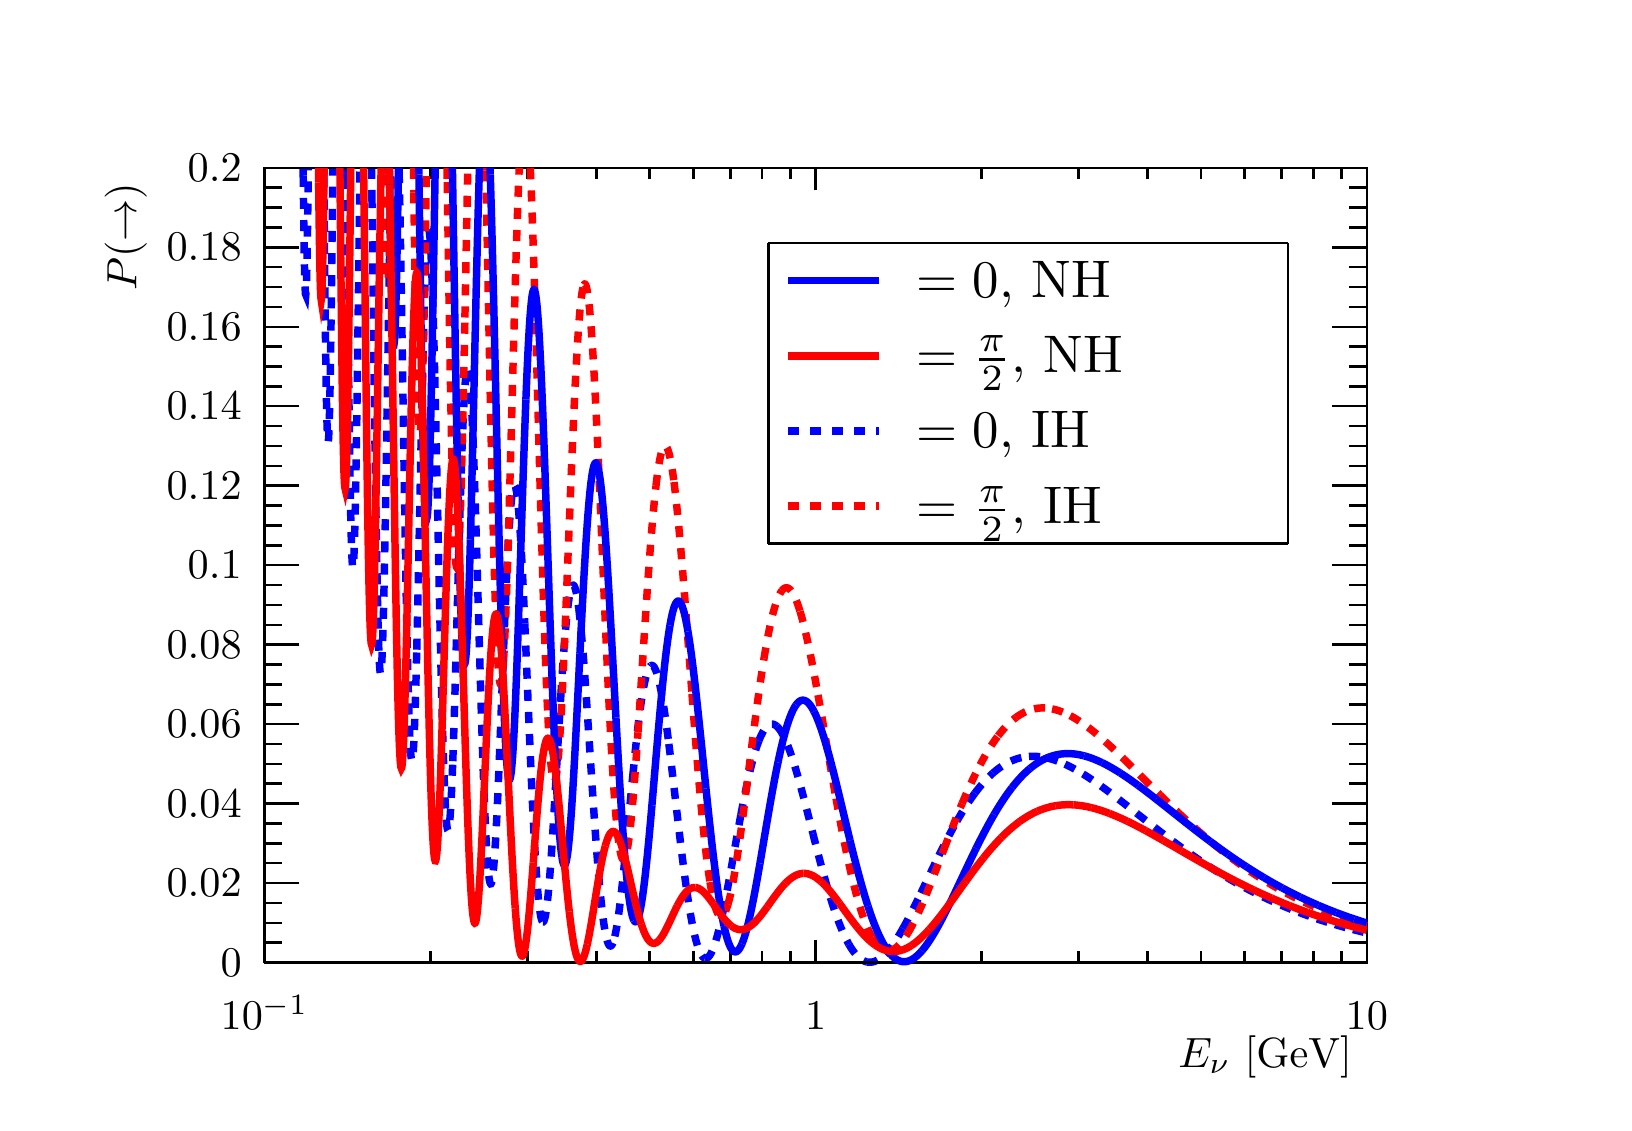
\begin{tikzpicture}
\pgfdeclareplotmark{cross} {
\pgfpathmoveto{\pgfpoint{-0.3\pgfplotmarksize}{\pgfplotmarksize}}
\pgfpathlineto{\pgfpoint{+0.3\pgfplotmarksize}{\pgfplotmarksize}}
\pgfpathlineto{\pgfpoint{+0.3\pgfplotmarksize}{0.3\pgfplotmarksize}}
\pgfpathlineto{\pgfpoint{+1\pgfplotmarksize}{0.3\pgfplotmarksize}}
\pgfpathlineto{\pgfpoint{+1\pgfplotmarksize}{-0.3\pgfplotmarksize}}
\pgfpathlineto{\pgfpoint{+0.3\pgfplotmarksize}{-0.3\pgfplotmarksize}}
\pgfpathlineto{\pgfpoint{+0.3\pgfplotmarksize}{-1.\pgfplotmarksize}}
\pgfpathlineto{\pgfpoint{-0.3\pgfplotmarksize}{-1.\pgfplotmarksize}}
\pgfpathlineto{\pgfpoint{-0.3\pgfplotmarksize}{-0.3\pgfplotmarksize}}
\pgfpathlineto{\pgfpoint{-1.\pgfplotmarksize}{-0.3\pgfplotmarksize}}
\pgfpathlineto{\pgfpoint{-1.\pgfplotmarksize}{0.3\pgfplotmarksize}}
\pgfpathlineto{\pgfpoint{-0.3\pgfplotmarksize}{0.3\pgfplotmarksize}}
\pgfpathclose
\pgfusepathqstroke
}
\pgfdeclareplotmark{cross*} {
\pgfpathmoveto{\pgfpoint{-0.3\pgfplotmarksize}{\pgfplotmarksize}}
\pgfpathlineto{\pgfpoint{+0.3\pgfplotmarksize}{\pgfplotmarksize}}
\pgfpathlineto{\pgfpoint{+0.3\pgfplotmarksize}{0.3\pgfplotmarksize}}
\pgfpathlineto{\pgfpoint{+1\pgfplotmarksize}{0.3\pgfplotmarksize}}
\pgfpathlineto{\pgfpoint{+1\pgfplotmarksize}{-0.3\pgfplotmarksize}}
\pgfpathlineto{\pgfpoint{+0.3\pgfplotmarksize}{-0.3\pgfplotmarksize}}
\pgfpathlineto{\pgfpoint{+0.3\pgfplotmarksize}{-1.\pgfplotmarksize}}
\pgfpathlineto{\pgfpoint{-0.3\pgfplotmarksize}{-1.\pgfplotmarksize}}
\pgfpathlineto{\pgfpoint{-0.3\pgfplotmarksize}{-0.3\pgfplotmarksize}}
\pgfpathlineto{\pgfpoint{-1.\pgfplotmarksize}{-0.3\pgfplotmarksize}}
\pgfpathlineto{\pgfpoint{-1.\pgfplotmarksize}{0.3\pgfplotmarksize}}
\pgfpathlineto{\pgfpoint{-0.3\pgfplotmarksize}{0.3\pgfplotmarksize}}
\pgfpathclose
\pgfusepathqfillstroke
}
\pgfdeclareplotmark{newstar} {
\pgfpathmoveto{\pgfqpoint{0pt}{\pgfplotmarksize}}
\pgfpathlineto{\pgfqpointpolar{44}{0.5\pgfplotmarksize}}
\pgfpathlineto{\pgfqpointpolar{18}{\pgfplotmarksize}}
\pgfpathlineto{\pgfqpointpolar{-20}{0.5\pgfplotmarksize}}
\pgfpathlineto{\pgfqpointpolar{-54}{\pgfplotmarksize}}
\pgfpathlineto{\pgfqpointpolar{-90}{0.5\pgfplotmarksize}}
\pgfpathlineto{\pgfqpointpolar{234}{\pgfplotmarksize}}
\pgfpathlineto{\pgfqpointpolar{198}{0.5\pgfplotmarksize}}
\pgfpathlineto{\pgfqpointpolar{162}{\pgfplotmarksize}}
\pgfpathlineto{\pgfqpointpolar{134}{0.5\pgfplotmarksize}}
\pgfpathclose
\pgfusepathqstroke
}
\pgfdeclareplotmark{newstar*} {
\pgfpathmoveto{\pgfqpoint{0pt}{\pgfplotmarksize}}
\pgfpathlineto{\pgfqpointpolar{44}{0.5\pgfplotmarksize}}
\pgfpathlineto{\pgfqpointpolar{18}{\pgfplotmarksize}}
\pgfpathlineto{\pgfqpointpolar{-20}{0.5\pgfplotmarksize}}
\pgfpathlineto{\pgfqpointpolar{-54}{\pgfplotmarksize}}
\pgfpathlineto{\pgfqpointpolar{-90}{0.5\pgfplotmarksize}}
\pgfpathlineto{\pgfqpointpolar{234}{\pgfplotmarksize}}
\pgfpathlineto{\pgfqpointpolar{198}{0.5\pgfplotmarksize}}
\pgfpathlineto{\pgfqpointpolar{162}{\pgfplotmarksize}}
\pgfpathlineto{\pgfqpointpolar{134}{0.5\pgfplotmarksize}}
\pgfpathclose
\pgfusepathqfillstroke
}
\definecolor{c}{rgb}{1,1,1};
\draw [color=c, fill=c] (0,0) rectangle (20,13.639);
\draw [color=c, fill=c] (3,1.77307) rectangle (17,11.8659);
\definecolor{c}{rgb}{0,0,0};
\draw [c,line width=0.9] (3,1.77307) -- (3,11.8659) -- (17,11.8659) -- (17,1.77307) -- (3,1.77307);
\definecolor{c}{rgb}{1,1,1};
\draw [color=c, fill=c] (3,1.77307) rectangle (17,11.8659);
\definecolor{c}{rgb}{0,0,0};
\draw [c,line width=0.9] (3,1.77307) -- (3,11.8659) -- (17,11.8659) -- (17,1.77307) -- (3,1.77307);
\definecolor{c}{rgb}{0,0,1};
\draw [c,dash pattern=on 4.00pt off 4.00pt ,line width=2.7] (3.49134,11.8659) -- (3.49233,11.7653);
\draw [c,dash pattern=on 4.00pt off 4.00pt ,line width=2.7] (3.49233,11.7653) -- (3.497,11.3524) -- (3.50167,11.0013) -- (3.50633,10.7152) -- (3.511,10.4963) -- (3.51567,10.3463) -- (3.52033,10.2657) -- (3.525,10.2545) -- (3.52967,10.3117) --
 (3.53433,10.4357) -- (3.539,10.624) -- (3.54367,10.8735) -- (3.54833,11.1803) -- (3.553,11.5399) -- (3.55673,11.8659);
\draw [c,dash pattern=on 4.00pt off 4.00pt ,line width=2.7] (3.7527,11.8659) -- (3.75367,11.7546);
\draw [c,dash pattern=on 4.00pt off 4.00pt ,line width=2.7] (3.75367,11.7546) -- (3.75833,11.244) -- (3.763,10.7647) -- (3.76767,10.3209) -- (3.77233,9.91617) -- (3.777,9.55399) -- (3.78167,9.23717) -- (3.78633,8.96812) -- (3.791,8.74873) --
 (3.79567,8.5804) -- (3.80033,8.46403) -- (3.805,8.4) -- (3.80967,8.38817) -- (3.81433,8.42791) -- (3.819,8.51812) -- (3.82367,8.65721) -- (3.82833,8.84314) -- (3.833,9.07346) -- (3.83767,9.34533) -- (3.84233,9.65554) -- (3.847,10.0005) --
 (3.85167,10.3765) -- (3.85633,10.7795) -- (3.861,11.205) -- (3.86567,11.6488) -- (3.86788,11.8659);
\draw [c,dash pattern=on 4.00pt off 4.00pt ,line width=2.7] (4.04177,11.8659) -- (4.043,11.7386);
\draw [c,dash pattern=on 4.00pt off 4.00pt ,line width=2.7] (4.043,11.7386) -- (4.04767,11.2611) -- (4.05233,10.7927) -- (4.057,10.3371) -- (4.06167,9.89744) -- (4.06633,9.47708) -- (4.071,9.079) -- (4.07567,8.70601) -- (4.08033,8.36069) --
 (4.085,8.04537) -- (4.08967,7.7621) -- (4.09433,7.51267) -- (4.099,7.29857) -- (4.10367,7.12101) -- (4.10833,6.98089) -- (4.113,6.87879) -- (4.11767,6.81501) -- (4.12233,6.78953) -- (4.127,6.80205) -- (4.13167,6.85195) -- (4.13633,6.93834) --
 (4.141,7.06007) -- (4.14567,7.21572) -- (4.15033,7.40361) -- (4.155,7.62185) -- (4.15967,7.86833) -- (4.16433,8.14076) -- (4.169,8.43666) -- (4.17367,8.75341) -- (4.17833,9.08826) -- (4.183,9.43834) -- (4.18767,9.80072) -- (4.19233,10.1724) --
 (4.197,10.5503) -- (4.20167,10.9315) -- (4.20633,11.3128) -- (4.211,11.6912) -- (4.21319,11.8659);
\draw [c,dash pattern=on 4.00pt off 4.00pt ,line width=2.7] (4.36041,11.8659) -- (4.365,11.496);
\draw [c,dash pattern=on 4.00pt off 4.00pt ,line width=2.7] (4.365,11.496) -- (4.36967,11.1138) -- (4.37433,10.7278) -- (4.379,10.3405) -- (4.38367,9.9544) -- (4.38833,9.57175) -- (4.393,9.19492) -- (4.39767,8.82616) -- (4.40233,8.46767) --
 (4.407,8.12155) -- (4.41167,7.78978) -- (4.41633,7.47426) -- (4.421,7.17673) -- (4.42567,6.89883) -- (4.43033,6.64203) -- (4.435,6.40767) -- (4.43967,6.19692) -- (4.44433,6.01079) -- (4.449,5.85013) -- (4.45367,5.71562) -- (4.45833,5.60777) --
 (4.463,5.5269) -- (4.46767,5.47319) -- (4.47233,5.44662) -- (4.477,5.44702) -- (4.48167,5.47406) -- (4.48633,5.52722) -- (4.491,5.60585) -- (4.49567,5.70915) -- (4.50033,5.83618) -- (4.505,5.98584) -- (4.50967,6.15695) -- (4.51433,6.34816) --
 (4.519,6.55806) -- (4.52367,6.78512) -- (4.52833,7.02772) -- (4.533,7.28418) -- (4.53767,7.55274) -- (4.54233,7.8316) -- (4.547,8.11891) -- (4.55167,8.4128) -- (4.55633,8.71136) -- (4.561,9.0127) -- (4.56567,9.31491) -- (4.57033,9.61612) --
 (4.575,9.91447) -- (4.57967,10.2081) -- (4.58433,10.4954) -- (4.589,10.7744);
\draw [c,dash pattern=on 4.00pt off 4.00pt ,line width=2.7] (4.589,10.7744) -- (4.59367,11.0436) -- (4.59833,11.3014) -- (4.603,11.5464) -- (4.60767,11.777) -- (4.6096,11.8659);
\draw [c,dash pattern=on 4.00pt off 4.00pt ,line width=2.7] (4.70909,11.8659) -- (4.71033,11.8102);
\draw [c,dash pattern=on 4.00pt off 4.00pt ,line width=2.7] (4.71033,11.8102) -- (4.715,11.586) -- (4.71967,11.3479) -- (4.72433,11.0972) -- (4.729,10.8352) -- (4.73367,10.5632) -- (4.73833,10.2827) -- (4.743,9.99506) -- (4.74767,9.70174) --
 (4.75233,9.40421) -- (4.757,9.10393) -- (4.76167,8.80237) -- (4.76633,8.501) -- (4.771,8.20125) -- (4.77567,7.90454) -- (4.78033,7.61227) -- (4.785,7.32578) -- (4.78967,7.04639) -- (4.79433,6.77536) -- (4.799,6.51389) -- (4.80367,6.26314) --
 (4.80833,6.02417) -- (4.813,5.79799) -- (4.81767,5.58556) -- (4.82233,5.38772) -- (4.827,5.20525) -- (4.83167,5.03884) -- (4.83633,4.88912) -- (4.841,4.75659) -- (4.84567,4.64169) -- (4.85033,4.54476) -- (4.855,4.46606) -- (4.85967,4.40575) --
 (4.86433,4.3639) -- (4.869,4.34049) -- (4.87367,4.33542) -- (4.87833,4.3485) -- (4.883,4.37945) -- (4.88767,4.42792) -- (4.89233,4.49347) -- (4.897,4.5756) -- (4.90167,4.67372) -- (4.90633,4.78719) -- (4.911,4.91528) -- (4.91567,5.05722) --
 (4.92033,5.21218) -- (4.925,5.37928) -- (4.92967,5.5576) -- (4.93433,5.74615);
\draw [c,dash pattern=on 4.00pt off 4.00pt ,line width=2.7] (4.93433,5.74615) -- (4.939,5.94394) -- (4.94367,6.14993) -- (4.94833,6.36305) -- (4.953,6.58222) -- (4.95767,6.80634) -- (4.96233,7.0343) -- (4.967,7.26498) -- (4.97167,7.49727) --
 (4.97633,7.73005) -- (4.981,7.96223) -- (4.98567,8.19271) -- (4.99033,8.42043) -- (4.995,8.64435) -- (4.99967,8.86344) -- (5.00433,9.07673) -- (5.009,9.28326) -- (5.01367,9.48212) -- (5.01833,9.67245) -- (5.023,9.85344) -- (5.02767,10.0243) --
 (5.03233,10.1843) -- (5.037,10.3328) -- (5.04167,10.4693) -- (5.04633,10.593) -- (5.051,10.7036) -- (5.05567,10.8006) -- (5.06033,10.8837) -- (5.065,10.9525) -- (5.06967,11.0068) -- (5.07433,11.0465) -- (5.079,11.0713) -- (5.08367,11.0813) --
 (5.08833,11.0765) -- (5.093,11.057) -- (5.09767,11.0228) -- (5.10233,10.9742) -- (5.107,10.9114) -- (5.11167,10.8348) -- (5.11633,10.7446) -- (5.121,10.6413) -- (5.12567,10.5253) -- (5.13033,10.3972) -- (5.135,10.2575) -- (5.13967,10.1068) --
 (5.14433,9.94565) -- (5.149,9.77481) -- (5.15367,9.59494) -- (5.15833,9.40675) -- (5.163,9.211);
\draw [c,dash pattern=on 4.00pt off 4.00pt ,line width=2.7] (5.163,9.211) -- (5.16767,9.00846) -- (5.17233,8.7999) -- (5.177,8.58615) -- (5.18167,8.36801) -- (5.18633,8.14631) -- (5.191,7.92187) -- (5.19567,7.69553) -- (5.20033,7.46812) --
 (5.205,7.24047) -- (5.20967,7.01339) -- (5.21433,6.78769) -- (5.219,6.56417) -- (5.22367,6.34361) -- (5.22833,6.12676) -- (5.233,5.91435) -- (5.23767,5.70711) -- (5.24233,5.50572) -- (5.247,5.31084) -- (5.25167,5.12309) -- (5.25633,4.94307) --
 (5.261,4.77133) -- (5.26567,4.6084) -- (5.27033,4.45477) -- (5.275,4.31087) -- (5.27967,4.17712) -- (5.28433,4.05388) -- (5.289,3.94147) -- (5.29367,3.84018) -- (5.29833,3.75024) -- (5.303,3.67185) -- (5.30767,3.60516) -- (5.31233,3.55027) --
 (5.317,3.50725) -- (5.32167,3.47613) -- (5.32633,3.45688) -- (5.331,3.44944) -- (5.33567,3.45372) -- (5.34033,3.46956) -- (5.345,3.49679) -- (5.34967,3.53519) -- (5.35433,3.58451) -- (5.359,3.64444) -- (5.36367,3.71468) -- (5.36833,3.79486) --
 (5.373,3.88461) -- (5.37767,3.98349) -- (5.38233,4.09108) -- (5.387,4.20691) -- (5.39167,4.33048);
\draw [c,dash pattern=on 4.00pt off 4.00pt ,line width=2.7] (5.39167,4.33048) -- (5.39633,4.46129) -- (5.401,4.59882) -- (5.40567,4.7425) -- (5.41033,4.89179) -- (5.415,5.04611) -- (5.41967,5.20487) -- (5.42433,5.36748) -- (5.429,5.53335) --
 (5.43367,5.70187) -- (5.43833,5.87243) -- (5.443,6.04443) -- (5.44767,6.21726) -- (5.45233,6.39033) -- (5.457,6.56304) -- (5.46167,6.73479) -- (5.46633,6.90502) -- (5.471,7.07315) -- (5.47567,7.23863) -- (5.48033,7.40092) -- (5.485,7.5595) --
 (5.48967,7.71385) -- (5.49433,7.8635) -- (5.499,8.00797) -- (5.50367,8.14681) -- (5.50833,8.27961) -- (5.513,8.40595) -- (5.51767,8.52547) -- (5.52233,8.63781) -- (5.527,8.74265) -- (5.53167,8.83968) -- (5.53633,8.92865) -- (5.541,9.00929) --
 (5.54567,9.0814) -- (5.55033,9.14479) -- (5.555,9.1993) -- (5.55967,9.2448) -- (5.56433,9.28119) -- (5.569,9.3084) -- (5.57367,9.32638) -- (5.57833,9.33512) -- (5.583,9.33462) -- (5.58767,9.32494) -- (5.59233,9.30612) -- (5.597,9.27828) --
 (5.60167,9.24152) -- (5.60633,9.19598) -- (5.611,9.14185) -- (5.61567,9.0793) -- (5.62033,9.00855);
\draw [c,dash pattern=on 4.00pt off 4.00pt ,line width=2.7] (5.62033,9.00855) -- (5.625,8.92984) -- (5.62967,8.84343) -- (5.63433,8.74958) -- (5.639,8.6486) -- (5.64367,8.5408) -- (5.64833,8.4265) -- (5.653,8.30605) -- (5.65767,8.17981) --
 (5.66233,8.04815) -- (5.667,7.91144) -- (5.67167,7.77009) -- (5.67633,7.6245) -- (5.681,7.47506) -- (5.68567,7.32221) -- (5.69033,7.16636) -- (5.695,7.00793) -- (5.69967,6.84736) -- (5.70433,6.68508) -- (5.709,6.5215) -- (5.71367,6.35707) --
 (5.71833,6.19221) -- (5.723,6.02735) -- (5.72767,5.8629) -- (5.73233,5.69928) -- (5.737,5.5369) -- (5.74167,5.37615) -- (5.74633,5.21743) -- (5.751,5.06113) -- (5.75567,4.90761) -- (5.76033,4.75723) -- (5.765,4.61035) -- (5.76967,4.4673) --
 (5.77433,4.32841) -- (5.779,4.19397) -- (5.78367,4.0643) -- (5.78833,3.93966) -- (5.793,3.82032) -- (5.79767,3.70653) -- (5.80233,3.59851) -- (5.807,3.49647) -- (5.81167,3.40062) -- (5.81633,3.31113) -- (5.821,3.22816) -- (5.82567,3.15185) --
 (5.83033,3.08232) -- (5.835,3.01968) -- (5.83967,2.96401) -- (5.84433,2.91538) -- (5.849,2.87384);
\draw [c,dash pattern=on 4.00pt off 4.00pt ,line width=2.7] (5.849,2.87384) -- (5.85367,2.83943) -- (5.85833,2.81215) -- (5.863,2.792) -- (5.86767,2.77896) -- (5.87233,2.77299) -- (5.877,2.77403) -- (5.88167,2.78202) -- (5.88633,2.79686) --
 (5.891,2.81844) -- (5.89567,2.84666) -- (5.90033,2.88136) -- (5.905,2.92242) -- (5.90967,2.96965) -- (5.91433,3.0229) -- (5.919,3.08196) -- (5.92367,3.14664) -- (5.92833,3.21673) -- (5.933,3.29201) -- (5.93767,3.37224) -- (5.94233,3.45718) --
 (5.947,3.54659) -- (5.95167,3.64021) -- (5.95633,3.73777) -- (5.961,3.839) -- (5.96567,3.94363) -- (5.97033,4.05138) -- (5.975,4.16195) -- (5.97967,4.27506) -- (5.98433,4.39042) -- (5.989,4.50774) -- (5.99367,4.62671) -- (5.99833,4.74705) --
 (6.003,4.86845) -- (6.00767,4.99062) -- (6.01233,5.11328) -- (6.017,5.23611) -- (6.02167,5.35884) -- (6.02633,5.48118) -- (6.031,5.60285) -- (6.03567,5.72357) -- (6.04033,5.84306) -- (6.045,5.96106) -- (6.04967,6.07731) -- (6.05433,6.19156) --
 (6.059,6.30354) -- (6.06367,6.41304) -- (6.06833,6.5198) -- (6.073,6.62361) -- (6.07767,6.72426);
\draw [c,dash pattern=on 4.00pt off 4.00pt ,line width=2.7] (6.07767,6.72426) -- (6.08233,6.82153) -- (6.087,6.91524) -- (6.09167,7.00518) -- (6.09633,7.09119) -- (6.101,7.1731) -- (6.10567,7.25075) -- (6.11033,7.32399) -- (6.115,7.3927) --
 (6.11967,7.45674) -- (6.12433,7.516) -- (6.129,7.57038) -- (6.13367,7.61979) -- (6.13833,7.66415) -- (6.143,7.70339) -- (6.14767,7.73746) -- (6.15233,7.7663) -- (6.157,7.78988) -- (6.16167,7.80818) -- (6.16633,7.82119) -- (6.171,7.82891) --
 (6.17567,7.83133) -- (6.18033,7.82849) -- (6.185,7.82041) -- (6.18967,7.80714) -- (6.19433,7.78871) -- (6.199,7.7652) -- (6.20367,7.73667) -- (6.20833,7.70321) -- (6.213,7.66489) -- (6.21767,7.62181) -- (6.22233,7.57408) -- (6.227,7.52181) --
 (6.23167,7.46513) -- (6.23633,7.40415) -- (6.241,7.33902) -- (6.24567,7.26987) -- (6.25033,7.19686) -- (6.255,7.12013) -- (6.25967,7.03985) -- (6.26433,6.95618) -- (6.269,6.86929) -- (6.27367,6.77935) -- (6.27833,6.68654) -- (6.283,6.59104) --
 (6.28767,6.49304) -- (6.29233,6.39272) -- (6.297,6.29027) -- (6.30167,6.18589) -- (6.30633,6.07977);
\draw [c,dash pattern=on 4.00pt off 4.00pt ,line width=2.7] (6.30633,6.07977) -- (6.311,5.9721) -- (6.31567,5.86308) -- (6.32033,5.7529) -- (6.325,5.64177) -- (6.32967,5.52987) -- (6.33433,5.4174) -- (6.339,5.30456) -- (6.34367,5.19155) --
 (6.34833,5.07854) -- (6.353,4.96574) -- (6.35767,4.85333) -- (6.36233,4.74149) -- (6.367,4.63041) -- (6.37167,4.52026) -- (6.37633,4.41123) -- (6.381,4.30348) -- (6.38567,4.19718) -- (6.39033,4.0925) -- (6.395,3.98959) -- (6.39967,3.88861) --
 (6.40433,3.78971) -- (6.409,3.69304) -- (6.41367,3.59872) -- (6.41833,3.5069) -- (6.423,3.41771) -- (6.42767,3.33127) -- (6.43233,3.24769) -- (6.437,3.16708) -- (6.44167,3.08956) -- (6.44633,3.01522) -- (6.451,2.94414) -- (6.45567,2.87642) --
 (6.46033,2.81214) -- (6.465,2.75136) -- (6.46967,2.69416) -- (6.47433,2.6406) -- (6.479,2.59072) -- (6.48367,2.54458) -- (6.48833,2.50221) -- (6.493,2.46365) -- (6.49767,2.42892) -- (6.50233,2.39805) -- (6.507,2.37104) -- (6.51167,2.34792) --
 (6.51633,2.32867) -- (6.521,2.3133) -- (6.52567,2.30178) -- (6.53033,2.29412) -- (6.535,2.29028);
\draw [c,dash pattern=on 4.00pt off 4.00pt ,line width=2.7] (6.535,2.29028) -- (6.53967,2.29023) -- (6.54433,2.29394) -- (6.549,2.30137) -- (6.55367,2.31248) -- (6.55833,2.32721) -- (6.563,2.34551) -- (6.56767,2.36732) -- (6.57233,2.39257) --
 (6.577,2.4212) -- (6.58167,2.45312) -- (6.58633,2.48826) -- (6.591,2.52654) -- (6.59567,2.56787) -- (6.60033,2.61215) -- (6.605,2.65931) -- (6.60967,2.70922) -- (6.61433,2.76181) -- (6.619,2.81696) -- (6.62367,2.87456) -- (6.62833,2.93451) --
 (6.633,2.9967) -- (6.63767,3.06101) -- (6.64233,3.12733) -- (6.647,3.19553) -- (6.65167,3.26551) -- (6.65633,3.33713) -- (6.661,3.41029) -- (6.66567,3.48485) -- (6.67033,3.56069) -- (6.675,3.63769) -- (6.67967,3.71573) -- (6.68433,3.79468) --
 (6.689,3.87441) -- (6.69367,3.95481) -- (6.69833,4.03574) -- (6.703,4.11708) -- (6.70767,4.19871) -- (6.71233,4.28052) -- (6.717,4.36237) -- (6.72167,4.44414) -- (6.72633,4.52573) -- (6.731,4.60701) -- (6.73567,4.68786) -- (6.74033,4.76818) --
 (6.745,4.84784) -- (6.74967,4.92675) -- (6.75433,5.00478) -- (6.759,5.08185) -- (6.76367,5.15784);
\draw [c,dash pattern=on 4.00pt off 4.00pt ,line width=2.7] (6.76367,5.15784) -- (6.76833,5.23265) -- (6.773,5.30619) -- (6.77767,5.37836) -- (6.78233,5.44907) -- (6.787,5.51823) -- (6.79167,5.58575) -- (6.79633,5.65155) -- (6.801,5.71555) --
 (6.80567,5.77767) -- (6.81033,5.83783) -- (6.815,5.89598) -- (6.81967,5.95203) -- (6.82433,6.00594) -- (6.829,6.05763) -- (6.83367,6.10704) -- (6.83833,6.15414) -- (6.843,6.19886) -- (6.84767,6.24116) -- (6.85233,6.28101) -- (6.857,6.31835) --
 (6.86167,6.35315) -- (6.86633,6.38539) -- (6.871,6.41504) -- (6.87567,6.44206) -- (6.88033,6.46644) -- (6.885,6.48817) -- (6.88967,6.50722) -- (6.89433,6.52359) -- (6.899,6.53728) -- (6.90367,6.54827) -- (6.90833,6.55656) -- (6.913,6.56217) --
 (6.91767,6.5651) -- (6.92233,6.56535) -- (6.927,6.56295) -- (6.93167,6.5579) -- (6.93633,6.55022) -- (6.941,6.53995) -- (6.94567,6.5271) -- (6.95033,6.51169) -- (6.955,6.49378) -- (6.95967,6.47337) -- (6.96433,6.45052) -- (6.969,6.42526) --
 (6.97367,6.39763) -- (6.97833,6.36768) -- (6.983,6.33545) -- (6.98767,6.30099) -- (6.99233,6.26435);
\draw [c,dash pattern=on 4.00pt off 4.00pt ,line width=2.7] (6.99233,6.26435) -- (6.997,6.22558) -- (7.00167,6.18475) -- (7.00633,6.14189) -- (7.011,6.09708) -- (7.01567,6.05037) -- (7.02033,6.00182) -- (7.025,5.9515) -- (7.02967,5.89947) --
 (7.03433,5.8458) -- (7.039,5.79055) -- (7.04367,5.7338) -- (7.04833,5.6756) -- (7.053,5.61603) -- (7.05767,5.55517) -- (7.06233,5.49308) -- (7.067,5.42984) -- (7.07167,5.36552) -- (7.07633,5.30019) -- (7.081,5.23392) -- (7.08567,5.1668) --
 (7.09033,5.09889) -- (7.095,5.03027) -- (7.09967,4.96102) -- (7.10433,4.8912) -- (7.109,4.8209) -- (7.11367,4.75019) -- (7.11833,4.67914) -- (7.123,4.60782) -- (7.12767,4.53632) -- (7.13233,4.46469) -- (7.137,4.39302) -- (7.14167,4.32138) --
 (7.14633,4.24983) -- (7.151,4.17845) -- (7.15567,4.1073) -- (7.16033,4.03646) -- (7.165,3.96598) -- (7.16967,3.89595) -- (7.17433,3.82641) -- (7.179,3.75745) -- (7.18367,3.68911) -- (7.18833,3.62146) -- (7.193,3.55457) -- (7.19767,3.48848) --
 (7.20233,3.42326) -- (7.207,3.35897) -- (7.21167,3.29565) -- (7.21633,3.23337) -- (7.221,3.17217);
\draw [c,dash pattern=on 4.00pt off 4.00pt ,line width=2.7] (7.221,3.17217) -- (7.22567,3.1121) -- (7.23033,3.05321) -- (7.235,2.99555) -- (7.23967,2.93916) -- (7.24433,2.88409) -- (7.249,2.83037) -- (7.25367,2.77806) -- (7.25833,2.72718) --
 (7.263,2.67777) -- (7.26767,2.62987) -- (7.27233,2.58351) -- (7.277,2.53872) -- (7.28167,2.49553) -- (7.28633,2.45397) -- (7.291,2.41406) -- (7.29567,2.37583) -- (7.30033,2.33929) -- (7.305,2.30447) -- (7.30967,2.27139) -- (7.31433,2.24007) --
 (7.319,2.21051) -- (7.32367,2.18273) -- (7.32833,2.15674) -- (7.333,2.13256) -- (7.33767,2.11018) -- (7.34233,2.08961) -- (7.347,2.07087) -- (7.35167,2.05394) -- (7.35633,2.03884) -- (7.361,2.02555) -- (7.36567,2.01409) -- (7.37033,2.00443) --
 (7.375,1.99659) -- (7.37967,1.99054) -- (7.38433,1.98628) -- (7.389,1.9838) -- (7.39367,1.98309) -- (7.39833,1.98414) -- (7.403,1.98692) -- (7.40767,1.99143) -- (7.41233,1.99764) -- (7.417,2.00554) -- (7.42167,2.0151) -- (7.42633,2.02631) --
 (7.431,2.03914) -- (7.43567,2.05357) -- (7.44033,2.06957) -- (7.445,2.08711) -- (7.44967,2.10618);
\draw [c,dash pattern=on 4.00pt off 4.00pt ,line width=2.7] (7.44967,2.10618) -- (7.45433,2.12673) -- (7.459,2.14875) -- (7.46367,2.17219) -- (7.46833,2.19704) -- (7.473,2.22325) -- (7.47767,2.2508) -- (7.48233,2.27964) -- (7.487,2.30975) --
 (7.49167,2.34109) -- (7.49633,2.37363) -- (7.501,2.40732) -- (7.50567,2.44214) -- (7.51033,2.47803) -- (7.515,2.51497) -- (7.51967,2.55292) -- (7.52433,2.59183) -- (7.529,2.63167) -- (7.53367,2.67239) -- (7.53833,2.71396) -- (7.543,2.75633) --
 (7.54767,2.79947) -- (7.55233,2.84333) -- (7.557,2.88788) -- (7.56167,2.93306) -- (7.56633,2.97884) -- (7.571,3.02518) -- (7.57567,3.07203) -- (7.58033,3.11936) -- (7.585,3.16712) -- (7.58967,3.21527) -- (7.59433,3.26376) -- (7.599,3.31257) --
 (7.60367,3.36164) -- (7.60833,3.41093) -- (7.613,3.46041) -- (7.61767,3.51003) -- (7.62233,3.55976) -- (7.627,3.60955) -- (7.63167,3.65936) -- (7.63633,3.70916) -- (7.641,3.7589) -- (7.64567,3.80855) -- (7.65033,3.85807) -- (7.655,3.90742) --
 (7.65967,3.95656) -- (7.66433,4.00547) -- (7.669,4.05409) -- (7.67367,4.1024) -- (7.67833,4.15037);
\draw [c,dash pattern=on 4.00pt off 4.00pt ,line width=2.7] (7.67833,4.15037) -- (7.683,4.19795) -- (7.68767,4.24511) -- (7.69233,4.29182) -- (7.697,4.33806) -- (7.70167,4.38378) -- (7.70633,4.42895) -- (7.711,4.47355) -- (7.71567,4.51755) --
 (7.72033,4.56091) -- (7.725,4.60362) -- (7.72967,4.64563) -- (7.73433,4.68693) -- (7.739,4.72749) -- (7.74367,4.76728) -- (7.74833,4.80628) -- (7.753,4.84447) -- (7.75767,4.88182) -- (7.76233,4.91831) -- (7.767,4.95392) -- (7.77167,4.98863) --
 (7.77633,5.02243) -- (7.781,5.05528) -- (7.78567,5.08718) -- (7.79033,5.11811) -- (7.795,5.14805) -- (7.79967,5.17698) -- (7.80433,5.2049) -- (7.809,5.23179) -- (7.81367,5.25763) -- (7.81833,5.28241) -- (7.823,5.30613) -- (7.82767,5.32877) --
 (7.83233,5.35032) -- (7.837,5.37077) -- (7.84167,5.39013) -- (7.84633,5.40837) -- (7.851,5.4255) -- (7.85567,5.4415) -- (7.86033,5.45638) -- (7.865,5.47012) -- (7.86967,5.48274) -- (7.87433,5.49422) -- (7.879,5.50456) -- (7.88367,5.51376) --
 (7.88833,5.52183) -- (7.893,5.52876) -- (7.89767,5.53455) -- (7.90233,5.53922) -- (7.907,5.54275);
\draw [c,dash pattern=on 4.00pt off 4.00pt ,line width=2.7] (7.907,5.54275) -- (7.91167,5.54516) -- (7.91633,5.54644) -- (7.921,5.54661) -- (7.92567,5.54567) -- (7.93033,5.54362) -- (7.935,5.54047) -- (7.93967,5.53624) -- (7.94433,5.53092) --
 (7.949,5.52453) -- (7.95367,5.51707) -- (7.95833,5.50857) -- (7.963,5.49901) -- (7.96767,5.48843) -- (7.97233,5.47683) -- (7.977,5.46421) -- (7.98167,5.45061) -- (7.98633,5.43602) -- (7.991,5.42046) -- (7.99567,5.40394) -- (8.00033,5.38649) --
 (8.005,5.36811) -- (8.00967,5.34882) -- (8.01433,5.32864) -- (8.019,5.30758) -- (8.02367,5.28565) -- (8.02833,5.26289) -- (8.033,5.23929) -- (8.03767,5.21489) -- (8.04233,5.18969) -- (8.047,5.16372) -- (8.05167,5.137) -- (8.05633,5.10954) --
 (8.061,5.08136) -- (8.06567,5.05248) -- (8.07033,5.02292) -- (8.075,4.99271) -- (8.07967,4.96185) -- (8.08433,4.93038) -- (8.089,4.89831) -- (8.09367,4.86566) -- (8.09833,4.83245) -- (8.103,4.7987) -- (8.10767,4.76444) -- (8.11233,4.72968) --
 (8.117,4.69444) -- (8.12167,4.65876) -- (8.12633,4.62264) -- (8.131,4.5861) -- (8.13567,4.54918);
\draw [c,dash pattern=on 4.00pt off 4.00pt ,line width=2.7] (8.13567,4.54918) -- (8.14033,4.51189) -- (8.145,4.47424) -- (8.14967,4.43628) -- (8.15433,4.398) -- (8.159,4.35944) -- (8.16367,4.32062) -- (8.16833,4.28155) -- (8.173,4.24227) --
 (8.17767,4.20278) -- (8.18233,4.16311) -- (8.187,4.12328) -- (8.19167,4.08331) -- (8.19633,4.04323) -- (8.201,4.00305) -- (8.20567,3.96279) -- (8.21033,3.92247) -- (8.215,3.88211) -- (8.21967,3.84174) -- (8.22433,3.80137) -- (8.229,3.76102) --
 (8.23367,3.72071) -- (8.23833,3.68046) -- (8.243,3.64028) -- (8.24767,3.60021) -- (8.25233,3.56025) -- (8.257,3.52042) -- (8.26167,3.48075) -- (8.26633,3.44124) -- (8.271,3.40192) -- (8.27567,3.36281) -- (8.28033,3.32392) -- (8.285,3.28526) --
 (8.28967,3.24686) -- (8.29433,3.20872) -- (8.299,3.17088) -- (8.30367,3.13333) -- (8.30833,3.0961) -- (8.313,3.05921) -- (8.31767,3.02266) -- (8.32233,2.98647) -- (8.327,2.95065) -- (8.33167,2.91523) -- (8.33633,2.8802) -- (8.341,2.8456) --
 (8.34567,2.81141) -- (8.35033,2.77768) -- (8.355,2.74439) -- (8.35967,2.71157) -- (8.36433,2.67922);
\draw [c,dash pattern=on 4.00pt off 4.00pt ,line width=2.7] (8.36433,2.67922) -- (8.369,2.64736) -- (8.37367,2.616) -- (8.37833,2.58515) -- (8.383,2.55482) -- (8.38767,2.52501) -- (8.39233,2.49575) -- (8.397,2.46703) -- (8.40167,2.43887) --
 (8.40633,2.41127) -- (8.411,2.38425) -- (8.41567,2.35781) -- (8.42033,2.33195) -- (8.425,2.3067) -- (8.42967,2.28204) -- (8.43433,2.25799) -- (8.439,2.23456) -- (8.44367,2.21175) -- (8.44833,2.18957) -- (8.453,2.16802) -- (8.45767,2.1471) --
 (8.46233,2.12683) -- (8.467,2.1072) -- (8.47167,2.08822) -- (8.47633,2.0699) -- (8.481,2.05223) -- (8.48567,2.03521) -- (8.49033,2.01886) -- (8.495,2.00318) -- (8.49967,1.98816) -- (8.50433,1.97381) -- (8.509,1.96012) -- (8.51367,1.94711) --
 (8.51833,1.93477) -- (8.523,1.9231) -- (8.52767,1.9121) -- (8.53233,1.90177) -- (8.537,1.89211) -- (8.54167,1.88313) -- (8.54633,1.87481) -- (8.551,1.86716) -- (8.55567,1.86018) -- (8.56033,1.85386) -- (8.565,1.84821) -- (8.56967,1.84322) --
 (8.57433,1.83889) -- (8.579,1.83521) -- (8.58367,1.83219) -- (8.58833,1.82981) -- (8.593,1.82808);
\draw [c,dash pattern=on 4.00pt off 4.00pt ,line width=2.7] (8.593,1.82808) -- (8.59767,1.827) -- (8.60233,1.82655) -- (8.607,1.82674) -- (8.61167,1.82755) -- (8.61633,1.829) -- (8.621,1.83106) -- (8.62567,1.83374) -- (8.63033,1.83703) --
 (8.635,1.84093) -- (8.63967,1.84542) -- (8.64433,1.85051) -- (8.649,1.85619) -- (8.65367,1.86245) -- (8.65833,1.86928) -- (8.663,1.87669) -- (8.66767,1.88465) -- (8.67233,1.89318) -- (8.677,1.90225) -- (8.68167,1.91186) -- (8.68633,1.92201) --
 (8.691,1.93269) -- (8.69567,1.94388) -- (8.70033,1.95559) -- (8.705,1.9678) -- (8.70967,1.98051) -- (8.71433,1.99371) -- (8.719,2.00739) -- (8.72367,2.02154) -- (8.72833,2.03615) -- (8.733,2.05123) -- (8.73767,2.06674) -- (8.74233,2.0827) --
 (8.747,2.09909) -- (8.75167,2.1159) -- (8.75633,2.13312) -- (8.761,2.15074) -- (8.76567,2.16876) -- (8.77033,2.18717) -- (8.775,2.20595) -- (8.77967,2.2251) -- (8.78433,2.2446) -- (8.789,2.26446) -- (8.79367,2.28466) -- (8.79833,2.30518) --
 (8.803,2.32603) -- (8.80767,2.34719) -- (8.81233,2.36866) -- (8.817,2.39041) -- (8.82167,2.41245);
\draw [c,dash pattern=on 4.00pt off 4.00pt ,line width=2.7] (8.82167,2.41245) -- (8.82633,2.43476) -- (8.831,2.45734) -- (8.83567,2.48018) -- (8.84033,2.50326) -- (8.845,2.52657) -- (8.84967,2.55011) -- (8.85433,2.57387) -- (8.859,2.59784) --
 (8.86367,2.62201) -- (8.86833,2.64636) -- (8.873,2.6709) -- (8.87767,2.69561) -- (8.88233,2.72047) -- (8.887,2.74549) -- (8.89167,2.77065) -- (8.89633,2.79595) -- (8.901,2.82137) -- (8.90567,2.8469) -- (8.91033,2.87254) -- (8.915,2.89828) --
 (8.91967,2.9241) -- (8.92433,2.95) -- (8.929,2.97598) -- (8.93367,3.00201) -- (8.93833,3.0281) -- (8.943,3.05423) -- (8.94767,3.08039) -- (8.95233,3.10658) -- (8.957,3.13279) -- (8.96167,3.15901) -- (8.96633,3.18522) -- (8.971,3.21143) --
 (8.97567,3.23763) -- (8.98033,3.2638) -- (8.985,3.28994) -- (8.98967,3.31604) -- (8.99433,3.34209) -- (8.999,3.36808) -- (9.00367,3.39401) -- (9.00833,3.41988) -- (9.013,3.44566) -- (9.01767,3.47135) -- (9.02233,3.49696) -- (9.027,3.52246) --
 (9.03167,3.54785) -- (9.03633,3.57313) -- (9.041,3.59829) -- (9.04567,3.62331) -- (9.05033,3.64821);
\draw [c,dash pattern=on 4.00pt off 4.00pt ,line width=2.7] (9.05033,3.64821) -- (9.055,3.67296) -- (9.05967,3.69756) -- (9.06433,3.722) -- (9.069,3.74629) -- (9.07367,3.7704) -- (9.07833,3.79435) -- (9.083,3.81811) -- (9.08767,3.84168) --
 (9.09233,3.86507) -- (9.097,3.88825) -- (9.10167,3.91123) -- (9.10633,3.93401) -- (9.111,3.95657) -- (9.11567,3.97891) -- (9.12033,4.00102) -- (9.125,4.02291) -- (9.12967,4.04456) -- (9.13433,4.06597) -- (9.139,4.08714) -- (9.14367,4.10806) --
 (9.14833,4.12872) -- (9.153,4.14913) -- (9.15767,4.16927) -- (9.16233,4.18915) -- (9.167,4.20876) -- (9.17167,4.2281) -- (9.17633,4.24715) -- (9.181,4.26593) -- (9.18567,4.28442) -- (9.19033,4.30262) -- (9.195,4.32053) -- (9.19967,4.33814) --
 (9.20433,4.35546) -- (9.209,4.37247) -- (9.21367,4.38918) -- (9.21833,4.40558) -- (9.223,4.42168) -- (9.22767,4.43746) -- (9.23233,4.45292) -- (9.237,4.46807) -- (9.24167,4.48289) -- (9.24633,4.4974) -- (9.251,4.51158) -- (9.25567,4.52544) --
 (9.26033,4.53896) -- (9.265,4.55216) -- (9.26967,4.56503) -- (9.27433,4.57756) -- (9.279,4.58976);
\draw [c,dash pattern=on 4.00pt off 4.00pt ,line width=2.7] (9.279,4.58976) -- (9.28367,4.60162) -- (9.28833,4.61315) -- (9.293,4.62434) -- (9.29767,4.63519) -- (9.30233,4.6457) -- (9.307,4.65587) -- (9.31167,4.6657) -- (9.31633,4.67518) --
 (9.321,4.68433) -- (9.32567,4.69313) -- (9.33033,4.70158) -- (9.335,4.7097) -- (9.33967,4.71746) -- (9.34433,4.72489) -- (9.349,4.73197) -- (9.35367,4.7387) -- (9.35833,4.7451) -- (9.363,4.75114) -- (9.36767,4.75685) -- (9.37233,4.76221) --
 (9.377,4.76723) -- (9.38167,4.77191) -- (9.38633,4.77624) -- (9.391,4.78024) -- (9.39567,4.78389) -- (9.40033,4.78721) -- (9.405,4.79019) -- (9.40967,4.79283) -- (9.41433,4.79514) -- (9.419,4.79711) -- (9.42367,4.79875) -- (9.42833,4.80005) --
 (9.433,4.80103) -- (9.43767,4.80168) -- (9.44233,4.802) -- (9.447,4.80199) -- (9.45167,4.80166) -- (9.45633,4.801) -- (9.461,4.80003) -- (9.46567,4.79873) -- (9.47033,4.79712) -- (9.475,4.7952) -- (9.47967,4.79296) -- (9.48433,4.79041) --
 (9.489,4.78755) -- (9.49367,4.78438) -- (9.49833,4.78091) -- (9.503,4.77714) -- (9.50767,4.77306);
\draw [c,dash pattern=on 4.00pt off 4.00pt ,line width=2.7] (9.50767,4.77306) -- (9.51233,4.76869) -- (9.517,4.76403) -- (9.52167,4.75907) -- (9.52633,4.75382) -- (9.531,4.74828) -- (9.53567,4.74246) -- (9.54033,4.73636) -- (9.545,4.72998) --
 (9.54967,4.72331) -- (9.55433,4.71638) -- (9.559,4.70917) -- (9.56367,4.7017) -- (9.56833,4.69396) -- (9.573,4.68596) -- (9.57767,4.6777) -- (9.58233,4.66918) -- (9.587,4.6604) -- (9.59167,4.65138) -- (9.59633,4.64211) -- (9.601,4.63259) --
 (9.60567,4.62283) -- (9.61033,4.61284) -- (9.615,4.60261) -- (9.61967,4.59214) -- (9.62433,4.58145) -- (9.629,4.57053) -- (9.63367,4.55939) -- (9.63833,4.54804) -- (9.643,4.53646) -- (9.64767,4.52467) -- (9.65233,4.51268) -- (9.657,4.50048) --
 (9.66167,4.48807) -- (9.66633,4.47547) -- (9.671,4.46267) -- (9.67567,4.44968) -- (9.68033,4.4365) -- (9.685,4.42314) -- (9.68967,4.40959) -- (9.69433,4.39586) -- (9.699,4.38196) -- (9.70367,4.36789) -- (9.70833,4.35365) -- (9.713,4.33925) --
 (9.71767,4.32468) -- (9.72233,4.30996) -- (9.727,4.29508) -- (9.73167,4.28005) -- (9.73633,4.26487);
\draw [c,dash pattern=on 4.00pt off 4.00pt ,line width=2.7] (9.73633,4.26487) -- (9.741,4.24955) -- (9.74567,4.23409) -- (9.75033,4.21849) -- (9.755,4.20276) -- (9.75967,4.1869) -- (9.76433,4.17091) -- (9.769,4.1548) -- (9.77367,4.13857) --
 (9.77833,4.12223) -- (9.783,4.10577) -- (9.78767,4.0892) -- (9.79233,4.07252) -- (9.797,4.05575) -- (9.80167,4.03887) -- (9.80633,4.0219) -- (9.811,4.00483) -- (9.81567,3.98768) -- (9.82033,3.97044) -- (9.825,3.95312) -- (9.82967,3.93572) --
 (9.83433,3.91825) -- (9.839,3.9007) -- (9.84367,3.88309) -- (9.84833,3.8654) -- (9.853,3.84766) -- (9.85767,3.82986) -- (9.86233,3.812) -- (9.867,3.79409) -- (9.87167,3.77612) -- (9.87633,3.75812) -- (9.881,3.74007) -- (9.88567,3.72198) --
 (9.89033,3.70385) -- (9.895,3.68569) -- (9.89967,3.6675) -- (9.90433,3.64928) -- (9.909,3.63104) -- (9.91367,3.61277) -- (9.91833,3.59449) -- (9.923,3.57619) -- (9.92767,3.55788) -- (9.93233,3.53956) -- (9.937,3.52123) -- (9.94167,3.5029) --
 (9.94633,3.48457) -- (9.951,3.46624) -- (9.95567,3.44791) -- (9.96033,3.42959) -- (9.965,3.41129);
\draw [c,dash pattern=on 4.00pt off 4.00pt ,line width=2.7] (9.965,3.41129) -- (9.96967,3.39299) -- (9.97433,3.37472) -- (9.979,3.35646) -- (9.98367,3.33822) -- (9.98833,3.32) -- (9.993,3.30182) -- (9.99767,3.28366) -- (10.0023,3.26553) --
 (10.007,3.24744) -- (10.0117,3.22938) -- (10.0163,3.21136) -- (10.021,3.19339) -- (10.0257,3.17546) -- (10.0303,3.15757) -- (10.035,3.13974) -- (10.0397,3.12195) -- (10.0443,3.10422) -- (10.049,3.08655) -- (10.0537,3.06893) -- (10.0583,3.05138) --
 (10.063,3.03388) -- (10.0677,3.01645) -- (10.0723,2.99909) -- (10.077,2.9818) -- (10.0817,2.96458) -- (10.0863,2.94743) -- (10.091,2.93036) -- (10.0957,2.91336) -- (10.1003,2.89645) -- (10.105,2.87961) -- (10.1097,2.86286) -- (10.1143,2.84619) --
 (10.119,2.82961) -- (10.1237,2.81312) -- (10.1283,2.79672) -- (10.133,2.78042) -- (10.1377,2.7642) -- (10.1423,2.74808) -- (10.147,2.73206) -- (10.1517,2.71614) -- (10.1563,2.70032) -- (10.161,2.6846) -- (10.1657,2.66899) -- (10.1703,2.65348) --
 (10.175,2.63808) -- (10.1797,2.62279) -- (10.1843,2.60761) -- (10.189,2.59254) -- (10.1937,2.57758);
\draw [c,dash pattern=on 4.00pt off 4.00pt ,line width=2.7] (10.1937,2.57758) -- (10.1983,2.56273) -- (10.203,2.54801) -- (10.2077,2.53339) -- (10.2123,2.5189) -- (10.217,2.50453) -- (10.2217,2.49028) -- (10.2263,2.47615) -- (10.231,2.46214) --
 (10.2357,2.44825) -- (10.2403,2.4345) -- (10.245,2.42087) -- (10.2497,2.40736) -- (10.2543,2.39399) -- (10.259,2.38074) -- (10.2637,2.36763) -- (10.2683,2.35464) -- (10.273,2.34179) -- (10.2777,2.32908) -- (10.2823,2.31649) -- (10.287,2.30405) --
 (10.2917,2.29174) -- (10.2963,2.27956) -- (10.301,2.26752) -- (10.3057,2.25563) -- (10.3103,2.24387) -- (10.315,2.23225) -- (10.3197,2.22077) -- (10.3243,2.20943) -- (10.329,2.19823) -- (10.3337,2.18718) -- (10.3383,2.17627) -- (10.343,2.1655) --
 (10.3477,2.15488) -- (10.3523,2.1444) -- (10.357,2.13407) -- (10.3617,2.12388) -- (10.3663,2.11384) -- (10.371,2.10394) -- (10.3757,2.09419) -- (10.3803,2.08459) -- (10.385,2.07514) -- (10.3897,2.06583) -- (10.3943,2.05667) -- (10.399,2.04766) --
 (10.4037,2.0388) -- (10.4083,2.03009) -- (10.413,2.02152) -- (10.4177,2.01311) -- (10.4223,2.00484);
\draw [c,dash pattern=on 4.00pt off 4.00pt ,line width=2.7] (10.4223,2.00484) -- (10.427,1.99673) -- (10.4317,1.98876) -- (10.4363,1.98094) -- (10.441,1.97328) -- (10.4457,1.96576) -- (10.4503,1.95839) -- (10.455,1.95118) -- (10.4597,1.94411) --
 (10.4643,1.9372) -- (10.469,1.93043) -- (10.4737,1.92381) -- (10.4783,1.91735) -- (10.483,1.91103) -- (10.4877,1.90486) -- (10.4923,1.89885) -- (10.497,1.89298) -- (10.5017,1.88726) -- (10.5063,1.88169) -- (10.511,1.87627) -- (10.5157,1.871) --
 (10.5203,1.86588) -- (10.525,1.8609) -- (10.5297,1.85607) -- (10.5343,1.85139) -- (10.539,1.84686) -- (10.5437,1.84248) -- (10.5483,1.83824) -- (10.553,1.83415) -- (10.5577,1.8302) -- (10.5623,1.8264) -- (10.567,1.82275) -- (10.5717,1.81924) --
 (10.5763,1.81588) -- (10.581,1.81265) -- (10.5857,1.80958) -- (10.5903,1.80664) -- (10.595,1.80385) -- (10.5997,1.80121) -- (10.6043,1.7987) -- (10.609,1.79633) -- (10.6137,1.79411) -- (10.6183,1.79203) -- (10.623,1.79008) -- (10.6277,1.78828) --
 (10.6323,1.78661) -- (10.637,1.78508) -- (10.6417,1.78369) -- (10.6463,1.78244) -- (10.651,1.78132);
\draw [c,dash pattern=on 4.00pt off 4.00pt ,line width=2.7] (10.651,1.78132) -- (10.6557,1.78034) -- (10.6603,1.77949) -- (10.665,1.77878) -- (10.6697,1.7782) -- (10.6743,1.77775) -- (10.679,1.77744) -- (10.6837,1.77726) -- (10.6883,1.77721) --
 (10.693,1.77729) -- (10.6977,1.7775) -- (10.7023,1.77784) -- (10.707,1.7783) -- (10.7117,1.7789) -- (10.7163,1.77962) -- (10.721,1.78047) -- (10.7257,1.78144) -- (10.7303,1.78253) -- (10.735,1.78376) -- (10.7397,1.7851) -- (10.7443,1.78657) --
 (10.749,1.78815) -- (10.7537,1.78986) -- (10.7583,1.79169) -- (10.763,1.79363) -- (10.7677,1.7957) -- (10.7723,1.79788) -- (10.777,1.80018) -- (10.7817,1.80259) -- (10.7863,1.80512) -- (10.791,1.80777) -- (10.7957,1.81052) -- (10.8003,1.81339) --
 (10.805,1.81637) -- (10.8097,1.81946) -- (10.8143,1.82266) -- (10.819,1.82597) -- (10.8237,1.82939) -- (10.8283,1.83291) -- (10.833,1.83654) -- (10.8377,1.84028) -- (10.8423,1.84412) -- (10.847,1.84806) -- (10.8517,1.85211) -- (10.8563,1.85625) --
 (10.861,1.8605) -- (10.8657,1.86485) -- (10.8703,1.8693) -- (10.875,1.87384) -- (10.8797,1.87849);
\draw [c,dash pattern=on 4.00pt off 4.00pt ,line width=2.7] (10.8797,1.87849) -- (10.8843,1.88322) -- (10.889,1.88806) -- (10.8937,1.89299) -- (10.8983,1.89801) -- (10.903,1.90312) -- (10.9077,1.90833) -- (10.9123,1.91362) -- (10.917,1.91901) --
 (10.9217,1.92448) -- (10.9263,1.93005) -- (10.931,1.9357) -- (10.9357,1.94143) -- (10.9403,1.94725) -- (10.945,1.95316) -- (10.9497,1.95914) -- (10.9543,1.96521) -- (10.959,1.97136) -- (10.9637,1.9776) -- (10.9683,1.98391) -- (10.973,1.9903) --
 (10.9777,1.99676) -- (10.9823,2.0033) -- (10.987,2.00992) -- (10.9917,2.01662) -- (10.9963,2.02338) -- (11.001,2.03022) -- (11.0057,2.03713) -- (11.0103,2.04412) -- (11.015,2.05117) -- (11.0197,2.05829) -- (11.0243,2.06548) -- (11.029,2.07274) --
 (11.0337,2.08006) -- (11.0383,2.08745) -- (11.043,2.0949) -- (11.0477,2.10241) -- (11.0523,2.10999) -- (11.057,2.11763) -- (11.0617,2.12533) -- (11.0663,2.13309) -- (11.071,2.14091) -- (11.0757,2.14879) -- (11.0803,2.15672) -- (11.085,2.16471) --
 (11.0897,2.17276) -- (11.0943,2.18086) -- (11.099,2.18901) -- (11.1037,2.19721) -- (11.1083,2.20547);
\draw [c,dash pattern=on 4.00pt off 4.00pt ,line width=2.7] (11.1083,2.20547) -- (11.113,2.21377) -- (11.1177,2.22213) -- (11.1223,2.23054) -- (11.127,2.23899) -- (11.1317,2.24749) -- (11.1363,2.25604) -- (11.141,2.26463) -- (11.1457,2.27326) --
 (11.1503,2.28194) -- (11.155,2.29066) -- (11.1597,2.29943) -- (11.1643,2.30823) -- (11.169,2.31708) -- (11.1737,2.32596) -- (11.1783,2.33488) -- (11.183,2.34384) -- (11.1877,2.35284) -- (11.1923,2.36187) -- (11.197,2.37094) -- (11.2017,2.38004) --
 (11.2063,2.38917) -- (11.211,2.39834) -- (11.2157,2.40754) -- (11.2203,2.41676) -- (11.225,2.42602) -- (11.2297,2.43531) -- (11.2343,2.44463) -- (11.239,2.45397) -- (11.2437,2.46334) -- (11.2483,2.47274) -- (11.253,2.48216) -- (11.2577,2.4916) --
 (11.2623,2.50107) -- (11.267,2.51056) -- (11.2717,2.52008) -- (11.2763,2.52961) -- (11.281,2.53917) -- (11.2857,2.54874) -- (11.2903,2.55834) -- (11.295,2.56795) -- (11.2997,2.57758) -- (11.3043,2.58722) -- (11.309,2.59688) -- (11.3137,2.60656) --
 (11.3183,2.61625) -- (11.323,2.62596) -- (11.3277,2.63568) -- (11.3323,2.64541) -- (11.337,2.65515);
\draw [c,dash pattern=on 4.00pt off 4.00pt ,line width=2.7] (11.337,2.65515) -- (11.3417,2.6649) -- (11.3463,2.67466) -- (11.351,2.68443) -- (11.3557,2.69422) -- (11.3603,2.704) -- (11.365,2.7138) -- (11.3697,2.7236) -- (11.3743,2.73341) --
 (11.379,2.74323) -- (11.3837,2.75305) -- (11.3883,2.76287) -- (11.393,2.77269) -- (11.3977,2.78252) -- (11.4023,2.79235) -- (11.407,2.80219) -- (11.4117,2.81202) -- (11.4163,2.82185) -- (11.421,2.83168) -- (11.4257,2.84152) -- (11.4303,2.85135) --
 (11.435,2.86117) -- (11.4397,2.871) -- (11.4443,2.88082) -- (11.449,2.89063) -- (11.4537,2.90045) -- (11.4583,2.91025) -- (11.463,2.92005) -- (11.4677,2.92985) -- (11.4723,2.93963) -- (11.477,2.94941) -- (11.4817,2.95918) -- (11.4863,2.96895) --
 (11.491,2.9787) -- (11.4957,2.98844) -- (11.5003,2.99817) -- (11.505,3.0079) -- (11.5097,3.01761) -- (11.5143,3.0273) -- (11.519,3.03699) -- (11.5237,3.04666) -- (11.5283,3.05632) -- (11.533,3.06597) -- (11.5377,3.0756) -- (11.5423,3.08521) --
 (11.547,3.09481) -- (11.5517,3.1044) -- (11.5563,3.11396) -- (11.561,3.12351) -- (11.5657,3.13305);
\draw [c,dash pattern=on 4.00pt off 4.00pt ,line width=2.7] (11.5657,3.13305) -- (11.5703,3.14256) -- (11.575,3.15206) -- (11.5797,3.16154) -- (11.5843,3.17099) -- (11.589,3.18043) -- (11.5937,3.18985) -- (11.5983,3.19925) -- (11.603,3.20863) --
 (11.6077,3.21798) -- (11.6123,3.22731) -- (11.617,3.23662) -- (11.6217,3.24591) -- (11.6263,3.25518) -- (11.631,3.26442) -- (11.6357,3.27364) -- (11.6403,3.28283) -- (11.645,3.292) -- (11.6497,3.30114) -- (11.6543,3.31026) -- (11.659,3.31935) --
 (11.6637,3.32841) -- (11.6683,3.33745) -- (11.673,3.34646) -- (11.6777,3.35545) -- (11.6823,3.3644) -- (11.687,3.37333) -- (11.6917,3.38223) -- (11.6963,3.3911) -- (11.701,3.39995) -- (11.7057,3.40876) -- (11.7103,3.41754) -- (11.715,3.42629) --
 (11.7197,3.43502) -- (11.7243,3.44371) -- (11.729,3.45237) -- (11.7337,3.461) -- (11.7383,3.4696) -- (11.743,3.47816) -- (11.7477,3.4867) -- (11.7523,3.4952) -- (11.757,3.50367) -- (11.7617,3.5121) -- (11.7663,3.5205) -- (11.771,3.52887) --
 (11.7757,3.53721) -- (11.7803,3.54551) -- (11.785,3.55377) -- (11.7897,3.56201) -- (11.7943,3.5702);
\draw [c,dash pattern=on 4.00pt off 4.00pt ,line width=2.7] (11.7943,3.5702) -- (11.799,3.57836) -- (11.8037,3.58649) -- (11.8083,3.59458) -- (11.813,3.60264) -- (11.8177,3.61065) -- (11.8223,3.61864) -- (11.827,3.62658) -- (11.8317,3.63449) --
 (11.8363,3.64236) -- (11.841,3.6502) -- (11.8457,3.658) -- (11.8503,3.66576) -- (11.855,3.67348) -- (11.8597,3.68116) -- (11.8643,3.68881) -- (11.869,3.69642) -- (11.8737,3.70399) -- (11.8783,3.71152) -- (11.883,3.71901) -- (11.8877,3.72647) --
 (11.8923,3.73388) -- (11.897,3.74125) -- (11.9017,3.74859) -- (11.9063,3.75589) -- (11.911,3.76314) -- (11.9157,3.77036) -- (11.9203,3.77753) -- (11.925,3.78467) -- (11.9297,3.79176) -- (11.9343,3.79882) -- (11.939,3.80583) -- (11.9437,3.8128) --
 (11.9483,3.81974) -- (11.953,3.82663) -- (11.9577,3.83348) -- (11.9623,3.84029) -- (11.967,3.84705) -- (11.9717,3.85378) -- (11.9763,3.86046) -- (11.981,3.86711) -- (11.9857,3.87371) -- (11.9903,3.88027) -- (11.995,3.88678) -- (11.9997,3.89326) --
 (12.0043,3.89969) -- (12.009,3.90608) -- (12.0137,3.91243) -- (12.0183,3.91874) -- (12.023,3.925);
\draw [c,dash pattern=on 4.00pt off 4.00pt ,line width=2.7] (12.023,3.925) -- (12.0277,3.93122) -- (12.0323,3.9374) -- (12.037,3.94353) -- (12.0417,3.94963) -- (12.0463,3.95568) -- (12.051,3.96168) -- (12.0557,3.96765) -- (12.0603,3.97357) --
 (12.065,3.97945) -- (12.0697,3.98528) -- (12.0743,3.99107) -- (12.079,3.99682) -- (12.0837,4.00253) -- (12.0883,4.00819) -- (12.093,4.01381) -- (12.0977,4.01939) -- (12.1023,4.02492) -- (12.107,4.03041) -- (12.1117,4.03586) -- (12.1163,4.04126) --
 (12.121,4.04662) -- (12.1257,4.05193) -- (12.1303,4.05721) -- (12.135,4.06244) -- (12.1397,4.06762) -- (12.1443,4.07276) -- (12.149,4.07786) -- (12.1537,4.08292) -- (12.1583,4.08793) -- (12.163,4.0929) -- (12.1677,4.09783) -- (12.1723,4.10271) --
 (12.177,4.10754) -- (12.1817,4.11234) -- (12.1863,4.11709) -- (12.191,4.1218) -- (12.1957,4.12646) -- (12.2003,4.13109) -- (12.205,4.13566) -- (12.2097,4.1402) -- (12.2143,4.14469) -- (12.219,4.14914) -- (12.2237,4.15355) -- (12.2283,4.15791) --
 (12.233,4.16223) -- (12.2377,4.1665) -- (12.2423,4.17074) -- (12.247,4.17493) -- (12.2517,4.17907);
\draw [c,dash pattern=on 4.00pt off 4.00pt ,line width=2.7] (12.2517,4.17907) -- (12.2563,4.18318) -- (12.261,4.18724) -- (12.2657,4.19126) -- (12.2703,4.19523) -- (12.275,4.19917) -- (12.2797,4.20306) -- (12.2843,4.20691) -- (12.289,4.21071) --
 (12.2937,4.21447) -- (12.2983,4.21819) -- (12.303,4.22187) -- (12.3077,4.22551) -- (12.3123,4.2291) -- (12.317,4.23265) -- (12.3217,4.23616) -- (12.3263,4.23963) -- (12.331,4.24306) -- (12.3357,4.24644) -- (12.3403,4.24978) -- (12.345,4.25308) --
 (12.3497,4.25634) -- (12.3543,4.25956) -- (12.359,4.26273) -- (12.3637,4.26587) -- (12.3683,4.26896) -- (12.373,4.27201) -- (12.3777,4.27502) -- (12.3823,4.27799) -- (12.387,4.28092) -- (12.3917,4.28381) -- (12.3963,4.28665) -- (12.401,4.28946) --
 (12.4057,4.29222) -- (12.4103,4.29495) -- (12.415,4.29763) -- (12.4197,4.30028) -- (12.4243,4.30288) -- (12.429,4.30545) -- (12.4337,4.30797) -- (12.4383,4.31045) -- (12.443,4.3129) -- (12.4477,4.3153) -- (12.4523,4.31767) -- (12.457,4.31999) --
 (12.4617,4.32228) -- (12.4663,4.32453) -- (12.471,4.32673) -- (12.4757,4.3289) -- (12.4803,4.33103);
\draw [c,dash pattern=on 4.00pt off 4.00pt ,line width=2.7] (12.4803,4.33103) -- (12.485,4.33312) -- (12.4897,4.33517) -- (12.4943,4.33719) -- (12.499,4.33916) -- (12.5037,4.3411) -- (12.5083,4.343) -- (12.513,4.34486) -- (12.5177,4.34668) --
 (12.5223,4.34846) -- (12.527,4.35021) -- (12.5317,4.35192) -- (12.5363,4.35359) -- (12.541,4.35522) -- (12.5457,4.35682) -- (12.5503,4.35838) -- (12.555,4.3599) -- (12.5597,4.36139) -- (12.5643,4.36284) -- (12.569,4.36425) -- (12.5737,4.36562) --
 (12.5783,4.36696) -- (12.583,4.36827) -- (12.5877,4.36953) -- (12.5923,4.37076) -- (12.597,4.37196) -- (12.6017,4.37312) -- (12.6063,4.37424) -- (12.611,4.37533) -- (12.6157,4.37638) -- (12.6203,4.3774) -- (12.625,4.37838) -- (12.6297,4.37933) --
 (12.6343,4.38024) -- (12.639,4.38112) -- (12.6437,4.38196) -- (12.6483,4.38277) -- (12.653,4.38355) -- (12.6577,4.38429) -- (12.6623,4.38499) -- (12.667,4.38567) -- (12.6717,4.3863) -- (12.6763,4.38691) -- (12.681,4.38748) -- (12.6857,4.38802) --
 (12.6903,4.38853) -- (12.695,4.389) -- (12.6997,4.38944) -- (12.7043,4.38984) -- (12.709,4.39022);
\draw [c,dash pattern=on 4.00pt off 4.00pt ,line width=2.7] (12.709,4.39022) -- (12.7137,4.39056) -- (12.7183,4.39087) -- (12.723,4.39115) -- (12.7277,4.39139) -- (12.7323,4.3916) -- (12.737,4.39179) -- (12.7417,4.39194) -- (12.7463,4.39205) --
 (12.751,4.39214) -- (12.7557,4.3922) -- (12.7603,4.39222) -- (12.765,4.39222) -- (12.7697,4.39218) -- (12.7743,4.39211) -- (12.779,4.39201) -- (12.7837,4.39189) -- (12.7883,4.39173) -- (12.793,4.39154) -- (12.7977,4.39132) -- (12.8023,4.39108) --
 (12.807,4.3908) -- (12.8117,4.39049) -- (12.8163,4.39015) -- (12.821,4.38979) -- (12.8257,4.3894) -- (12.8303,4.38897) -- (12.835,4.38852) -- (12.8397,4.38804) -- (12.8443,4.38753) -- (12.849,4.387) -- (12.8537,4.38643) -- (12.8583,4.38584) --
 (12.863,4.38522) -- (12.8677,4.38457) -- (12.8723,4.38389) -- (12.877,4.38319) -- (12.8817,4.38246) -- (12.8863,4.3817) -- (12.891,4.38092) -- (12.8957,4.3801) -- (12.9003,4.37927) -- (12.905,4.3784) -- (12.9097,4.37751) -- (12.9143,4.37659) --
 (12.919,4.37565) -- (12.9237,4.37468) -- (12.9283,4.37369) -- (12.933,4.37267) -- (12.9377,4.37162);
\draw [c,dash pattern=on 4.00pt off 4.00pt ,line width=2.7] (12.9377,4.37162) -- (12.9423,4.37055) -- (12.947,4.36945) -- (12.9517,4.36833) -- (12.9563,4.36719) -- (12.961,4.36601) -- (12.9657,4.36482) -- (12.9703,4.3636) -- (12.975,4.36235) --
 (12.9797,4.36109) -- (12.9843,4.35979) -- (12.989,4.35848) -- (12.9937,4.35714) -- (12.9983,4.35577) -- (13.003,4.35439) -- (13.0077,4.35298) -- (13.0123,4.35154) -- (13.017,4.35008) -- (13.0217,4.34861) -- (13.0263,4.3471) -- (13.031,4.34558) --
 (13.0357,4.34403) -- (13.0403,4.34246) -- (13.045,4.34087) -- (13.0497,4.33926) -- (13.0543,4.33762) -- (13.059,4.33596) -- (13.0637,4.33428) -- (13.0683,4.33258) -- (13.073,4.33086) -- (13.0777,4.32912) -- (13.0823,4.32735) -- (13.087,4.32557) --
 (13.0917,4.32376) -- (13.0963,4.32194) -- (13.101,4.32009) -- (13.1057,4.31823) -- (13.1103,4.31634) -- (13.115,4.31443) -- (13.1197,4.3125) -- (13.1243,4.31056) -- (13.129,4.30859) -- (13.1337,4.3066) -- (13.1383,4.3046) -- (13.143,4.30257) --
 (13.1477,4.30053) -- (13.1523,4.29847) -- (13.157,4.29639) -- (13.1617,4.29429) -- (13.1663,4.29217);
\draw [c,dash pattern=on 4.00pt off 4.00pt ,line width=2.7] (13.1663,4.29217) -- (13.171,4.29003) -- (13.1757,4.28788) -- (13.1803,4.2857) -- (13.185,4.28351) -- (13.1897,4.2813) -- (13.1943,4.27907) -- (13.199,4.27683) -- (13.2037,4.27457) --
 (13.2083,4.27229) -- (13.213,4.26999) -- (13.2177,4.26768) -- (13.2223,4.26535) -- (13.227,4.263) -- (13.2317,4.26063) -- (13.2363,4.25825) -- (13.241,4.25586) -- (13.2457,4.25344) -- (13.2503,4.25101) -- (13.255,4.24857) -- (13.2597,4.2461) --
 (13.2643,4.24363) -- (13.269,4.24113) -- (13.2737,4.23862) -- (13.2783,4.2361) -- (13.283,4.23356) -- (13.2877,4.23101) -- (13.2923,4.22844) -- (13.297,4.22585) -- (13.3017,4.22325) -- (13.3063,4.22064) -- (13.311,4.21801) -- (13.3157,4.21537) --
 (13.3203,4.21271) -- (13.325,4.21004) -- (13.3297,4.20735) -- (13.3343,4.20465) -- (13.339,4.20194) -- (13.3437,4.19921) -- (13.3483,4.19647) -- (13.353,4.19372) -- (13.3577,4.19095) -- (13.3623,4.18817) -- (13.367,4.18537) -- (13.3717,4.18257) --
 (13.3763,4.17975) -- (13.381,4.17692) -- (13.3857,4.17407) -- (13.3903,4.17121) -- (13.395,4.16834);
\draw [c,dash pattern=on 4.00pt off 4.00pt ,line width=2.7] (13.395,4.16834) -- (13.3997,4.16546) -- (13.4043,4.16257) -- (13.409,4.15966) -- (13.4137,4.15674) -- (13.4183,4.15381) -- (13.423,4.15087) -- (13.4277,4.14792) -- (13.4323,4.14495) --
 (13.437,4.14197) -- (13.4417,4.13899) -- (13.4463,4.13599) -- (13.451,4.13298) -- (13.4557,4.12996) -- (13.4603,4.12693) -- (13.465,4.12389) -- (13.4697,4.12083) -- (13.4743,4.11777) -- (13.479,4.1147) -- (13.4837,4.11161) -- (13.4883,4.10852) --
 (13.493,4.10541) -- (13.4977,4.1023) -- (13.5023,4.09918) -- (13.507,4.09604) -- (13.5117,4.0929) -- (13.5163,4.08975) -- (13.521,4.08658) -- (13.5257,4.08341) -- (13.5303,4.08023) -- (13.535,4.07704) -- (13.5397,4.07384) -- (13.5443,4.07063) --
 (13.549,4.06742) -- (13.5537,4.06419) -- (13.5583,4.06096) -- (13.563,4.05772) -- (13.5677,4.05446) -- (13.5723,4.05121) -- (13.577,4.04794) -- (13.5817,4.04466) -- (13.5863,4.04138) -- (13.591,4.03809) -- (13.5957,4.03479) -- (13.6003,4.03148) --
 (13.605,4.02817) -- (13.6097,4.02484) -- (13.6143,4.02152) -- (13.619,4.01818) -- (13.6237,4.01483);
\draw [c,dash pattern=on 4.00pt off 4.00pt ,line width=2.7] (13.6237,4.01483) -- (13.6283,4.01148) -- (13.633,4.00812) -- (13.6377,4.00476) -- (13.6423,4.00139) -- (13.647,3.99801) -- (13.6517,3.99462) -- (13.6563,3.99123) -- (13.661,3.98783) --
 (13.6657,3.98443) -- (13.6703,3.98101) -- (13.675,3.9776) -- (13.6797,3.97417) -- (13.6843,3.97074) -- (13.689,3.96731) -- (13.6937,3.96386) -- (13.6983,3.96042) -- (13.703,3.95696) -- (13.7077,3.9535) -- (13.7123,3.95004) -- (13.717,3.94657) --
 (13.7217,3.94309) -- (13.7263,3.93961) -- (13.731,3.93613) -- (13.7357,3.93264) -- (13.7403,3.92914) -- (13.745,3.92564) -- (13.7497,3.92213) -- (13.7543,3.91862) -- (13.759,3.91511) -- (13.7637,3.91159) -- (13.7683,3.90806) -- (13.773,3.90453) --
 (13.7777,3.901) -- (13.7823,3.89746) -- (13.787,3.89392) -- (13.7917,3.89037) -- (13.7963,3.88682) -- (13.801,3.88327) -- (13.8057,3.87971) -- (13.8103,3.87615) -- (13.815,3.87258) -- (13.8197,3.86901) -- (13.8243,3.86544) -- (13.829,3.86186) --
 (13.8337,3.85828) -- (13.8383,3.8547) -- (13.843,3.85111) -- (13.8477,3.84752) -- (13.8523,3.84393);
\draw [c,dash pattern=on 4.00pt off 4.00pt ,line width=2.7] (13.8523,3.84393) -- (13.857,3.84033) -- (13.8617,3.83673) -- (13.8663,3.83313) -- (13.871,3.82953) -- (13.8757,3.82592) -- (13.8803,3.82231) -- (13.885,3.81869) -- (13.8897,3.81508) --
 (13.8943,3.81146) -- (13.899,3.80784) -- (13.9037,3.80422) -- (13.9083,3.80059) -- (13.913,3.79696) -- (13.9177,3.79333) -- (13.9223,3.7897) -- (13.927,3.78607) -- (13.9317,3.78243) -- (13.9363,3.77879) -- (13.941,3.77515) -- (13.9457,3.77151) --
 (13.9503,3.76787) -- (13.955,3.76422) -- (13.9597,3.76057) -- (13.9643,3.75693) -- (13.969,3.75328) -- (13.9737,3.74962) -- (13.9783,3.74597) -- (13.983,3.74232) -- (13.9877,3.73866) -- (13.9923,3.73501) -- (13.997,3.73135) -- (14.0017,3.72769) --
 (14.0063,3.72403) -- (14.011,3.72037) -- (14.0157,3.71671) -- (14.0203,3.71305) -- (14.025,3.70938) -- (14.0297,3.70572) -- (14.0343,3.70206) -- (14.039,3.69839) -- (14.0437,3.69473) -- (14.0483,3.69106) -- (14.053,3.68739) -- (14.0577,3.68373) --
 (14.0623,3.68006) -- (14.067,3.67639) -- (14.0717,3.67273) -- (14.0763,3.66906) -- (14.081,3.66539);
\draw [c,dash pattern=on 4.00pt off 4.00pt ,line width=2.7] (14.081,3.66539) -- (14.0857,3.66173) -- (14.0903,3.65806) -- (14.095,3.65439) -- (14.0997,3.65072) -- (14.1043,3.64706) -- (14.109,3.64339) -- (14.1137,3.63972) -- (14.1183,3.63606) --
 (14.123,3.63239) -- (14.1277,3.62873) -- (14.1323,3.62506) -- (14.137,3.6214) -- (14.1417,3.61773) -- (14.1463,3.61407) -- (14.151,3.61041) -- (14.1557,3.60675) -- (14.1603,3.60309) -- (14.165,3.59943) -- (14.1697,3.59577) -- (14.1743,3.59211) --
 (14.179,3.58845) -- (14.1837,3.58479) -- (14.1883,3.58114) -- (14.193,3.57749) -- (14.1977,3.57383) -- (14.2023,3.57018) -- (14.207,3.56653) -- (14.2117,3.56288) -- (14.2163,3.55923) -- (14.221,3.55559) -- (14.2257,3.55194) -- (14.2303,3.5483) --
 (14.235,3.54466) -- (14.2397,3.54102) -- (14.2443,3.53738) -- (14.249,3.53374) -- (14.2537,3.5301) -- (14.2583,3.52647) -- (14.263,3.52284) -- (14.2677,3.51921) -- (14.2723,3.51558) -- (14.277,3.51195) -- (14.2817,3.50833) -- (14.2863,3.5047) --
 (14.291,3.50108) -- (14.2957,3.49747) -- (14.3003,3.49385) -- (14.305,3.49023) -- (14.3097,3.48662);
\draw [c,dash pattern=on 4.00pt off 4.00pt ,line width=2.7] (14.3097,3.48662) -- (14.3143,3.48301) -- (14.319,3.4794) -- (14.3237,3.4758) -- (14.3283,3.47219) -- (14.333,3.46859) -- (14.3377,3.46499) -- (14.3423,3.4614) -- (14.347,3.4578) --
 (14.3517,3.45421) -- (14.3563,3.45062) -- (14.361,3.44704) -- (14.3657,3.44345) -- (14.3703,3.43987) -- (14.375,3.43629) -- (14.3797,3.43272) -- (14.3843,3.42915) -- (14.389,3.42558) -- (14.3937,3.42201) -- (14.3983,3.41844) -- (14.403,3.41488) --
 (14.4077,3.41132) -- (14.4123,3.40777) -- (14.417,3.40421) -- (14.4217,3.40066) -- (14.4263,3.39711) -- (14.431,3.39357) -- (14.4357,3.39003) -- (14.4403,3.38649) -- (14.445,3.38296) -- (14.4497,3.37942) -- (14.4543,3.3759) -- (14.459,3.37237) --
 (14.4637,3.36885) -- (14.4683,3.36533) -- (14.473,3.36181) -- (14.4777,3.3583) -- (14.4823,3.35479) -- (14.487,3.35129) -- (14.4917,3.34778) -- (14.4963,3.34429) -- (14.501,3.34079) -- (14.5057,3.3373) -- (14.5103,3.33381) -- (14.515,3.33033) --
 (14.5197,3.32684) -- (14.5243,3.32337) -- (14.529,3.31989) -- (14.5337,3.31642) -- (14.5383,3.31296);
\draw [c,dash pattern=on 4.00pt off 4.00pt ,line width=2.7] (14.5383,3.31296) -- (14.543,3.30949) -- (14.5477,3.30603) -- (14.5523,3.30258) -- (14.557,3.29913) -- (14.5617,3.29568) -- (14.5663,3.29223) -- (14.571,3.28879) -- (14.5757,3.28536) --
 (14.5803,3.28192) -- (14.585,3.2785) -- (14.5897,3.27507) -- (14.5943,3.27165) -- (14.599,3.26823) -- (14.6037,3.26482) -- (14.6083,3.26141) -- (14.613,3.25801) -- (14.6177,3.2546) -- (14.6223,3.25121) -- (14.627,3.24781) -- (14.6317,3.24443) --
 (14.6363,3.24104) -- (14.641,3.23766) -- (14.6457,3.23429) -- (14.6503,3.23091) -- (14.655,3.22755) -- (14.6597,3.22418) -- (14.6643,3.22082) -- (14.669,3.21747) -- (14.6737,3.21412) -- (14.6783,3.21077) -- (14.683,3.20743) -- (14.6877,3.20409) --
 (14.6923,3.20076) -- (14.697,3.19743) -- (14.7017,3.1941) -- (14.7063,3.19078) -- (14.711,3.18747) -- (14.7157,3.18415) -- (14.7203,3.18085) -- (14.725,3.17754) -- (14.7297,3.17425) -- (14.7343,3.17095) -- (14.739,3.16766) -- (14.7437,3.16438) --
 (14.7483,3.1611) -- (14.753,3.15782) -- (14.7577,3.15455) -- (14.7623,3.15129) -- (14.767,3.14803);
\draw [c,dash pattern=on 4.00pt off 4.00pt ,line width=2.7] (14.767,3.14803) -- (14.7717,3.14477) -- (14.7763,3.14152) -- (14.781,3.13827) -- (14.7857,3.13503) -- (14.7903,3.13179) -- (14.795,3.12855) -- (14.7997,3.12532) -- (14.8043,3.1221) --
 (14.809,3.11888) -- (14.8137,3.11567) -- (14.8183,3.11246) -- (14.823,3.10925) -- (14.8277,3.10605) -- (14.8323,3.10285) -- (14.837,3.09966) -- (14.8417,3.09648) -- (14.8463,3.0933) -- (14.851,3.09012) -- (14.8557,3.08695) -- (14.8603,3.08378) --
 (14.865,3.08062) -- (14.8697,3.07746) -- (14.8743,3.07431) -- (14.879,3.07116) -- (14.8837,3.06802) -- (14.8883,3.06488) -- (14.893,3.06175) -- (14.8977,3.05862) -- (14.9023,3.0555) -- (14.907,3.05238) -- (14.9117,3.04927) -- (14.9163,3.04616) --
 (14.921,3.04306) -- (14.9257,3.03996) -- (14.9303,3.03687) -- (14.935,3.03378) -- (14.9397,3.0307) -- (14.9443,3.02762) -- (14.949,3.02455) -- (14.9537,3.02148) -- (14.9583,3.01842) -- (14.963,3.01536) -- (14.9677,3.01231) -- (14.9723,3.00926) --
 (14.977,3.00622) -- (14.9817,3.00319) -- (14.9863,3.00015) -- (14.991,2.99713) -- (14.9957,2.99411);
\draw [c,dash pattern=on 4.00pt off 4.00pt ,line width=2.7] (14.9957,2.99411) -- (15.0003,2.99109) -- (15.005,2.98808) -- (15.0097,2.98507) -- (15.0143,2.98207) -- (15.019,2.97907) -- (15.0237,2.97608) -- (15.0283,2.9731) -- (15.033,2.97012) --
 (15.0377,2.96714) -- (15.0423,2.96417) -- (15.047,2.96121) -- (15.0517,2.95825) -- (15.0563,2.95529) -- (15.061,2.95234) -- (15.0657,2.9494) -- (15.0703,2.94646) -- (15.075,2.94353) -- (15.0797,2.9406) -- (15.0843,2.93768) -- (15.089,2.93476) --
 (15.0937,2.93185) -- (15.0983,2.92894) -- (15.103,2.92604) -- (15.1077,2.92314) -- (15.1123,2.92025) -- (15.117,2.91736) -- (15.1217,2.91448) -- (15.1263,2.9116) -- (15.131,2.90873) -- (15.1357,2.90587) -- (15.1403,2.90301) -- (15.145,2.90015) --
 (15.1497,2.8973) -- (15.1543,2.89446) -- (15.159,2.89162) -- (15.1637,2.88879) -- (15.1683,2.88596) -- (15.173,2.88314) -- (15.1777,2.88032) -- (15.1823,2.8775) -- (15.187,2.8747) -- (15.1917,2.8719) -- (15.1963,2.8691) -- (15.201,2.86631) --
 (15.2057,2.86352) -- (15.2103,2.86074) -- (15.215,2.85797) -- (15.2197,2.8552) -- (15.2243,2.85243);
\draw [c,dash pattern=on 4.00pt off 4.00pt ,line width=2.7] (15.2243,2.85243) -- (15.229,2.84967) -- (15.2337,2.84692) -- (15.2383,2.84417) -- (15.243,2.84142) -- (15.2477,2.83869) -- (15.2523,2.83595) -- (15.257,2.83323) -- (15.2617,2.8305) --
 (15.2663,2.82779) -- (15.271,2.82507) -- (15.2757,2.82237) -- (15.2803,2.81967) -- (15.285,2.81697) -- (15.2897,2.81428) -- (15.2943,2.8116) -- (15.299,2.80892) -- (15.3037,2.80624) -- (15.3083,2.80357) -- (15.313,2.80091) -- (15.3177,2.79825) --
 (15.3223,2.7956) -- (15.327,2.79295) -- (15.3317,2.79031) -- (15.3363,2.78767) -- (15.341,2.78504) -- (15.3457,2.78241) -- (15.3503,2.77979) -- (15.355,2.77717) -- (15.3597,2.77456) -- (15.3643,2.77196) -- (15.369,2.76936) -- (15.3737,2.76676) --
 (15.3783,2.76417) -- (15.383,2.76159) -- (15.3877,2.75901) -- (15.3923,2.75644) -- (15.397,2.75387) -- (15.4017,2.75131) -- (15.4063,2.74875) -- (15.411,2.7462) -- (15.4157,2.74365) -- (15.4203,2.74111) -- (15.425,2.73857) -- (15.4297,2.73604) --
 (15.4343,2.73352) -- (15.439,2.73099) -- (15.4437,2.72848) -- (15.4483,2.72597) -- (15.453,2.72346);
\draw [c,dash pattern=on 4.00pt off 4.00pt ,line width=2.7] (15.453,2.72346) -- (15.4577,2.72096) -- (15.4623,2.71847) -- (15.467,2.71598) -- (15.4717,2.7135) -- (15.4763,2.71102) -- (15.481,2.70855) -- (15.4857,2.70608) -- (15.4903,2.70362) --
 (15.495,2.70116) -- (15.4997,2.69871) -- (15.5043,2.69626) -- (15.509,2.69382) -- (15.5137,2.69138) -- (15.5183,2.68895) -- (15.523,2.68652) -- (15.5277,2.6841) -- (15.5323,2.68169) -- (15.537,2.67928) -- (15.5417,2.67687) -- (15.5463,2.67447) --
 (15.551,2.67208) -- (15.5557,2.66969) -- (15.5603,2.6673) -- (15.565,2.66492) -- (15.5697,2.66255) -- (15.5743,2.66018) -- (15.579,2.65782) -- (15.5837,2.65546) -- (15.5883,2.65311) -- (15.593,2.65076) -- (15.5977,2.64842) -- (15.6023,2.64608) --
 (15.607,2.64375) -- (15.6117,2.64142) -- (15.6163,2.6391) -- (15.621,2.63678) -- (15.6257,2.63447) -- (15.6303,2.63216) -- (15.635,2.62986) -- (15.6397,2.62756) -- (15.6443,2.62527) -- (15.649,2.62298) -- (15.6537,2.6207) -- (15.6583,2.61843) --
 (15.663,2.61616) -- (15.6677,2.61389) -- (15.6723,2.61163) -- (15.677,2.60937) -- (15.6817,2.60712);
\draw [c,dash pattern=on 4.00pt off 4.00pt ,line width=2.7] (15.6817,2.60712) -- (15.6863,2.60488) -- (15.691,2.60264) -- (15.6957,2.6004) -- (15.7003,2.59817) -- (15.705,2.59594) -- (15.7097,2.59372) -- (15.7143,2.59151) -- (15.719,2.5893) --
 (15.7237,2.58709) -- (15.7283,2.58489) -- (15.733,2.5827) -- (15.7377,2.58051) -- (15.7423,2.57832) -- (15.747,2.57614) -- (15.7517,2.57397) -- (15.7563,2.5718) -- (15.761,2.56963) -- (15.7657,2.56747) -- (15.7703,2.56532) -- (15.775,2.56317) --
 (15.7797,2.56102) -- (15.7843,2.55888) -- (15.789,2.55675) -- (15.7937,2.55462) -- (15.7983,2.55249) -- (15.803,2.55037) -- (15.8077,2.54825) -- (15.8123,2.54614) -- (15.817,2.54404) -- (15.8217,2.54194) -- (15.8263,2.53984) -- (15.831,2.53775) --
 (15.8357,2.53566) -- (15.8403,2.53358) -- (15.845,2.53151) -- (15.8497,2.52943) -- (15.8543,2.52737) -- (15.859,2.52531) -- (15.8637,2.52325) -- (15.8683,2.5212) -- (15.873,2.51915) -- (15.8777,2.51711) -- (15.8823,2.51507) -- (15.887,2.51304) --
 (15.8917,2.51101) -- (15.8963,2.50899) -- (15.901,2.50697) -- (15.9057,2.50495) -- (15.9103,2.50294);
\draw [c,dash pattern=on 4.00pt off 4.00pt ,line width=2.7] (15.9103,2.50294) -- (15.915,2.50094) -- (15.9197,2.49894) -- (15.9243,2.49695) -- (15.929,2.49496) -- (15.9337,2.49297) -- (15.9383,2.49099) -- (15.943,2.48902) -- (15.9477,2.48705) --
 (15.9523,2.48508) -- (15.957,2.48312) -- (15.9617,2.48116) -- (15.9663,2.47921) -- (15.971,2.47726) -- (15.9757,2.47532) -- (15.9803,2.47338) -- (15.985,2.47145) -- (15.9897,2.46952) -- (15.9943,2.4676) -- (15.999,2.46568) -- (16.0037,2.46376) --
 (16.0083,2.46185) -- (16.013,2.45995) -- (16.0177,2.45805) -- (16.0223,2.45615) -- (16.027,2.45426) -- (16.0317,2.45237) -- (16.0363,2.45049) -- (16.041,2.44861) -- (16.0457,2.44674) -- (16.0503,2.44487) -- (16.055,2.44301) -- (16.0597,2.44115) --
 (16.0643,2.43929) -- (16.069,2.43744) -- (16.0737,2.4356) -- (16.0783,2.43376) -- (16.083,2.43192) -- (16.0877,2.43009) -- (16.0923,2.42826) -- (16.097,2.42644) -- (16.1017,2.42462) -- (16.1063,2.4228) -- (16.111,2.42099) -- (16.1157,2.41919) --
 (16.1203,2.41739) -- (16.125,2.41559) -- (16.1297,2.4138) -- (16.1343,2.41201) -- (16.139,2.41023);
\draw [c,dash pattern=on 4.00pt off 4.00pt ,line width=2.7] (16.139,2.41023) -- (16.1437,2.40845) -- (16.1483,2.40668) -- (16.153,2.40491) -- (16.1577,2.40314) -- (16.1623,2.40138) -- (16.167,2.39963) -- (16.1717,2.39787) -- (16.1763,2.39613) --
 (16.181,2.39438) -- (16.1857,2.39264) -- (16.1903,2.39091) -- (16.195,2.38918) -- (16.1997,2.38745) -- (16.2043,2.38573) -- (16.209,2.38401) -- (16.2137,2.3823) -- (16.2183,2.38059) -- (16.223,2.37889) -- (16.2277,2.37719) -- (16.2323,2.37549) --
 (16.237,2.3738) -- (16.2417,2.37211) -- (16.2463,2.37043) -- (16.251,2.36875) -- (16.2557,2.36708) -- (16.2603,2.36541) -- (16.265,2.36374) -- (16.2697,2.36208) -- (16.2743,2.36042) -- (16.279,2.35877) -- (16.2837,2.35712) -- (16.2883,2.35547) --
 (16.293,2.35383) -- (16.2977,2.3522) -- (16.3023,2.35056) -- (16.307,2.34893) -- (16.3117,2.34731) -- (16.3163,2.34569) -- (16.321,2.34407) -- (16.3257,2.34246) -- (16.3303,2.34086) -- (16.335,2.33925) -- (16.3397,2.33765) -- (16.3443,2.33606) --
 (16.349,2.33447) -- (16.3537,2.33288) -- (16.3583,2.3313) -- (16.363,2.32972) -- (16.3677,2.32814);
\draw [c,dash pattern=on 4.00pt off 4.00pt ,line width=2.7] (16.3677,2.32814) -- (16.3723,2.32657) -- (16.377,2.325) -- (16.3817,2.32344) -- (16.3863,2.32188) -- (16.391,2.32033) -- (16.3957,2.31878) -- (16.4003,2.31723) -- (16.405,2.31569) --
 (16.4097,2.31415) -- (16.4143,2.31261) -- (16.419,2.31108) -- (16.4237,2.30955) -- (16.4283,2.30803) -- (16.433,2.30651) -- (16.4377,2.305) -- (16.4423,2.30349) -- (16.447,2.30198) -- (16.4517,2.30048) -- (16.4563,2.29898) -- (16.461,2.29748) --
 (16.4657,2.29599) -- (16.4703,2.2945) -- (16.475,2.29302) -- (16.4797,2.29154) -- (16.4843,2.29006) -- (16.489,2.28859) -- (16.4937,2.28712) -- (16.4983,2.28566) -- (16.503,2.28419) -- (16.5077,2.28274) -- (16.5123,2.28128) -- (16.517,2.27983) --
 (16.5217,2.27839) -- (16.5263,2.27695) -- (16.531,2.27551) -- (16.5357,2.27408) -- (16.5403,2.27264) -- (16.545,2.27122) -- (16.5497,2.2698) -- (16.5543,2.26838) -- (16.559,2.26696) -- (16.5637,2.26555) -- (16.5683,2.26414) -- (16.573,2.26274) --
 (16.5777,2.26134) -- (16.5823,2.25994) -- (16.587,2.25855) -- (16.5917,2.25716) -- (16.5963,2.25577);
\draw [c,dash pattern=on 4.00pt off 4.00pt ,line width=2.7] (16.5963,2.25577) -- (16.601,2.25439) -- (16.6057,2.25301) -- (16.6103,2.25163) -- (16.615,2.25026) -- (16.6197,2.2489) -- (16.6243,2.24753) -- (16.629,2.24617) -- (16.6337,2.24481) --
 (16.6383,2.24346) -- (16.643,2.24211) -- (16.6477,2.24077) -- (16.6523,2.23942) -- (16.657,2.23808) -- (16.6617,2.23675) -- (16.6663,2.23542) -- (16.671,2.23409) -- (16.6757,2.23276) -- (16.6803,2.23144) -- (16.685,2.23013) -- (16.6897,2.22881) --
 (16.6943,2.2275) -- (16.699,2.22619) -- (16.7037,2.22489) -- (16.7083,2.22359) -- (16.713,2.22229) -- (16.7177,2.221) -- (16.7223,2.21971) -- (16.727,2.21842) -- (16.7317,2.21714) -- (16.7363,2.21586) -- (16.741,2.21459) -- (16.7457,2.21331) --
 (16.7503,2.21204) -- (16.755,2.21078) -- (16.7597,2.20952) -- (16.7643,2.20826) -- (16.769,2.207) -- (16.7737,2.20575) -- (16.7783,2.2045) -- (16.783,2.20326) -- (16.7877,2.20201) -- (16.7923,2.20077) -- (16.797,2.19954) -- (16.8017,2.19831) --
 (16.8063,2.19708) -- (16.811,2.19585) -- (16.8157,2.19463) -- (16.8203,2.19341) -- (16.825,2.1922);
\draw [c,dash pattern=on 4.00pt off 4.00pt ,line width=2.7] (16.825,2.1922) -- (16.8297,2.19099) -- (16.8343,2.18978) -- (16.839,2.18857) -- (16.8437,2.18737) -- (16.8483,2.18617) -- (16.853,2.18497) -- (16.8577,2.18378) -- (16.8623,2.18259) --
 (16.867,2.18141) -- (16.8717,2.18022) -- (16.8763,2.17904) -- (16.881,2.17787) -- (16.8857,2.17669) -- (16.8903,2.17552) -- (16.895,2.17436) -- (16.8997,2.17319) -- (16.9043,2.17203) -- (16.909,2.17087) -- (16.9137,2.16972) -- (16.9183,2.16857) --
 (16.923,2.16742) -- (16.9277,2.16628) -- (16.9323,2.16513) -- (16.937,2.164) -- (16.9417,2.16286) -- (16.9463,2.16173) -- (16.951,2.1606) -- (16.9557,2.15947) -- (16.9603,2.15835) -- (16.965,2.15723) -- (16.9697,2.15611) -- (16.9743,2.155) --
 (16.979,2.15389) -- (16.9837,2.15278) -- (16.9883,2.15168) -- (16.993,2.15057) -- (16.9977,2.14947);
\definecolor{c}{rgb}{0,0,0};
\draw [c,line width=0.9] (3,1.77307) -- (17,1.77307);
\draw [c,line width=0.9] (3.00001,2.05948) -- (3.00001,1.77307);
\draw [anchor=base] (3.00001,0.92063) node[scale=1.52731, color=c, rotate=0]{$10^{-1}$};
\draw [c,line width=0.9] (5.10722,1.91628) -- (5.10722,1.77307);
\draw [c,line width=0.9] (6.33985,1.91628) -- (6.33985,1.77307);
\draw [c,line width=0.9] (7.21442,1.91628) -- (7.21442,1.77307);
\draw [c,line width=0.9] (7.89279,1.91628) -- (7.89279,1.77307);
\draw [c,line width=0.9] (8.44706,1.91628) -- (8.44706,1.77307);
\draw [c,line width=0.9] (8.91569,1.91628) -- (8.91569,1.77307);
\draw [c,line width=0.9] (9.32163,1.91628) -- (9.32163,1.77307);
\draw [c,line width=0.9] (9.6797,1.91628) -- (9.6797,1.77307);
\draw [c,line width=0.9] (10,2.05948) -- (10,1.77307);
\draw [anchor=base] (10,0.92063) node[scale=1.52731, color=c, rotate=0]{1};
\draw [c,line width=0.9] (12.1072,1.91628) -- (12.1072,1.77307);
\draw [c,line width=0.9] (13.3399,1.91628) -- (13.3399,1.77307);
\draw [c,line width=0.9] (14.2144,1.91628) -- (14.2144,1.77307);
\draw [c,line width=0.9] (14.8928,1.91628) -- (14.8928,1.77307);
\draw [c,line width=0.9] (15.4471,1.91628) -- (15.4471,1.77307);
\draw [c,line width=0.9] (15.9157,1.91628) -- (15.9157,1.77307);
\draw [c,line width=0.9] (16.3216,1.91628) -- (16.3216,1.77307);
\draw [c,line width=0.9] (16.6797,1.91628) -- (16.6797,1.77307);
\draw [c,line width=0.9] (17,2.05948) -- (17,1.77307);
\draw [anchor=base] (17,0.92063) node[scale=1.52731, color=c, rotate=0]{10};
\draw [anchor= east] (17,0.572837) node[scale=1.52731, color=c, rotate=0]{$E_{\nu}$ [GeV]};
\draw [c,line width=0.9] (3,11.8659) -- (17,11.8659);
\draw [c,line width=0.9] (3.00001,11.5795) -- (3.00001,11.8659);
\draw [c,line width=0.9] (5.10722,11.7227) -- (5.10722,11.8659);
\draw [c,line width=0.9] (6.33985,11.7227) -- (6.33985,11.8659);
\draw [c,line width=0.9] (7.21442,11.7227) -- (7.21442,11.8659);
\draw [c,line width=0.9] (7.89279,11.7227) -- (7.89279,11.8659);
\draw [c,line width=0.9] (8.44706,11.7227) -- (8.44706,11.8659);
\draw [c,line width=0.9] (8.91569,11.7227) -- (8.91569,11.8659);
\draw [c,line width=0.9] (9.32163,11.7227) -- (9.32163,11.8659);
\draw [c,line width=0.9] (9.6797,11.7227) -- (9.6797,11.8659);
\draw [c,line width=0.9] (10,11.5795) -- (10,11.8659);
\draw [c,line width=0.9] (12.1072,11.7227) -- (12.1072,11.8659);
\draw [c,line width=0.9] (13.3399,11.7227) -- (13.3399,11.8659);
\draw [c,line width=0.9] (14.2144,11.7227) -- (14.2144,11.8659);
\draw [c,line width=0.9] (14.8928,11.7227) -- (14.8928,11.8659);
\draw [c,line width=0.9] (15.4471,11.7227) -- (15.4471,11.8659);
\draw [c,line width=0.9] (15.9157,11.7227) -- (15.9157,11.8659);
\draw [c,line width=0.9] (16.3216,11.7227) -- (16.3216,11.8659);
\draw [c,line width=0.9] (16.6797,11.7227) -- (16.6797,11.8659);
\draw [c,line width=0.9] (17,11.5795) -- (17,11.8659);
\draw [c,line width=0.9] (3,1.77307) -- (3,11.8659);
\draw [c,line width=0.9] (3.444,1.77307) -- (3,1.77307);
\draw [c,line width=0.9] (3.222,2.02539) -- (3,2.02539);
\draw [c,line width=0.9] (3.222,2.27771) -- (3,2.27771);
\draw [c,line width=0.9] (3.222,2.53003) -- (3,2.53003);
\draw [c,line width=0.9] (3.444,2.78235) -- (3,2.78235);
\draw [c,line width=0.9] (3.222,3.03467) -- (3,3.03467);
\draw [c,line width=0.9] (3.222,3.28699) -- (3,3.28699);
\draw [c,line width=0.9] (3.222,3.53931) -- (3,3.53931);
\draw [c,line width=0.9] (3.444,3.79163) -- (3,3.79163);
\draw [c,line width=0.9] (3.222,4.04395) -- (3,4.04395);
\draw [c,line width=0.9] (3.222,4.29628) -- (3,4.29628);
\draw [c,line width=0.9] (3.222,4.5486) -- (3,4.5486);
\draw [c,line width=0.9] (3.444,4.80092) -- (3,4.80092);
\draw [c,line width=0.9] (3.222,5.05324) -- (3,5.05324);
\draw [c,line width=0.9] (3.222,5.30556) -- (3,5.30556);
\draw [c,line width=0.9] (3.222,5.55788) -- (3,5.55788);
\draw [c,line width=0.9] (3.444,5.8102) -- (3,5.8102);
\draw [c,line width=0.9] (3.222,6.06252) -- (3,6.06252);
\draw [c,line width=0.9] (3.222,6.31484) -- (3,6.31484);
\draw [c,line width=0.9] (3.222,6.56716) -- (3,6.56716);
\draw [c,line width=0.9] (3.444,6.81948) -- (3,6.81948);
\draw [c,line width=0.9] (3.222,7.07181) -- (3,7.07181);
\draw [c,line width=0.9] (3.222,7.32413) -- (3,7.32413);
\draw [c,line width=0.9] (3.222,7.57645) -- (3,7.57645);
\draw [c,line width=0.9] (3.444,7.82877) -- (3,7.82877);
\draw [c,line width=0.9] (3.222,8.08109) -- (3,8.08109);
\draw [c,line width=0.9] (3.222,8.33341) -- (3,8.33341);
\draw [c,line width=0.9] (3.222,8.58573) -- (3,8.58573);
\draw [c,line width=0.9] (3.444,8.83805) -- (3,8.83805);
\draw [c,line width=0.9] (3.222,9.09037) -- (3,9.09037);
\draw [c,line width=0.9] (3.222,9.34269) -- (3,9.34269);
\draw [c,line width=0.9] (3.222,9.59501) -- (3,9.59501);
\draw [c,line width=0.9] (3.444,9.84733) -- (3,9.84733);
\draw [c,line width=0.9] (3.222,10.0997) -- (3,10.0997);
\draw [c,line width=0.9] (3.222,10.352) -- (3,10.352);
\draw [c,line width=0.9] (3.222,10.6043) -- (3,10.6043);
\draw [c,line width=0.9] (3.444,10.8566) -- (3,10.8566);
\draw [c,line width=0.9] (3.222,11.1089) -- (3,11.1089);
\draw [c,line width=0.9] (3.222,11.3613) -- (3,11.3613);
\draw [c,line width=0.9] (3.222,11.6136) -- (3,11.6136);
\draw [c,line width=0.9] (3.444,11.8659) -- (3,11.8659);
\draw [anchor= east] (2.9,1.77307) node[scale=1.52731, color=c, rotate=0]{0};
\draw [anchor= east] (2.9,2.78235) node[scale=1.52731, color=c, rotate=0]{0.02};
\draw [anchor= east] (2.9,3.79163) node[scale=1.52731, color=c, rotate=0]{0.04};
\draw [anchor= east] (2.9,4.80092) node[scale=1.52731, color=c, rotate=0]{0.06};
\draw [anchor= east] (2.9,5.8102) node[scale=1.52731, color=c, rotate=0]{0.08};
\draw [anchor= east] (2.9,6.81948) node[scale=1.52731, color=c, rotate=0]{0.1};
\draw [anchor= east] (2.9,7.82877) node[scale=1.52731, color=c, rotate=0]{0.12};
\draw [anchor= east] (2.9,8.83805) node[scale=1.52731, color=c, rotate=0]{0.14};
\draw [anchor= east] (2.9,9.84733) node[scale=1.52731, color=c, rotate=0]{0.16};
\draw [anchor= east] (2.9,10.8566) node[scale=1.52731, color=c, rotate=0]{0.18};
\draw [anchor= east] (2.9,11.8659) node[scale=1.52731, color=c, rotate=0]{0.2};
\draw [anchor= east] (1.24,11.8659) node[scale=1.52731, color=c, rotate=90]{$P(\numu \rightarrow \nue)$};
\draw [c,line width=0.9] (17,1.77307) -- (17,11.8659);
\draw [c,line width=0.9] (16.556,1.77307) -- (17,1.77307);
\draw [c,line width=0.9] (16.778,2.02539) -- (17,2.02539);
\draw [c,line width=0.9] (16.778,2.27771) -- (17,2.27771);
\draw [c,line width=0.9] (16.778,2.53003) -- (17,2.53003);
\draw [c,line width=0.9] (16.556,2.78235) -- (17,2.78235);
\draw [c,line width=0.9] (16.778,3.03467) -- (17,3.03467);
\draw [c,line width=0.9] (16.778,3.28699) -- (17,3.28699);
\draw [c,line width=0.9] (16.778,3.53931) -- (17,3.53931);
\draw [c,line width=0.9] (16.556,3.79163) -- (17,3.79163);
\draw [c,line width=0.9] (16.778,4.04395) -- (17,4.04395);
\draw [c,line width=0.9] (16.778,4.29628) -- (17,4.29628);
\draw [c,line width=0.9] (16.778,4.5486) -- (17,4.5486);
\draw [c,line width=0.9] (16.556,4.80092) -- (17,4.80092);
\draw [c,line width=0.9] (16.778,5.05324) -- (17,5.05324);
\draw [c,line width=0.9] (16.778,5.30556) -- (17,5.30556);
\draw [c,line width=0.9] (16.778,5.55788) -- (17,5.55788);
\draw [c,line width=0.9] (16.556,5.8102) -- (17,5.8102);
\draw [c,line width=0.9] (16.778,6.06252) -- (17,6.06252);
\draw [c,line width=0.9] (16.778,6.31484) -- (17,6.31484);
\draw [c,line width=0.9] (16.778,6.56716) -- (17,6.56716);
\draw [c,line width=0.9] (16.556,6.81948) -- (17,6.81948);
\draw [c,line width=0.9] (16.778,7.07181) -- (17,7.07181);
\draw [c,line width=0.9] (16.778,7.32413) -- (17,7.32413);
\draw [c,line width=0.9] (16.778,7.57645) -- (17,7.57645);
\draw [c,line width=0.9] (16.556,7.82877) -- (17,7.82877);
\draw [c,line width=0.9] (16.778,8.08109) -- (17,8.08109);
\draw [c,line width=0.9] (16.778,8.33341) -- (17,8.33341);
\draw [c,line width=0.9] (16.778,8.58573) -- (17,8.58573);
\draw [c,line width=0.9] (16.556,8.83805) -- (17,8.83805);
\draw [c,line width=0.9] (16.778,9.09037) -- (17,9.09037);
\draw [c,line width=0.9] (16.778,9.34269) -- (17,9.34269);
\draw [c,line width=0.9] (16.778,9.59501) -- (17,9.59501);
\draw [c,line width=0.9] (16.556,9.84733) -- (17,9.84733);
\draw [c,line width=0.9] (16.778,10.0997) -- (17,10.0997);
\draw [c,line width=0.9] (16.778,10.352) -- (17,10.352);
\draw [c,line width=0.9] (16.778,10.6043) -- (17,10.6043);
\draw [c,line width=0.9] (16.556,10.8566) -- (17,10.8566);
\draw [c,line width=0.9] (16.778,11.1089) -- (17,11.1089);
\draw [c,line width=0.9] (16.778,11.3613) -- (17,11.3613);
\draw [c,line width=0.9] (16.778,11.6136) -- (17,11.6136);
\draw [c,line width=0.9] (16.556,11.8659) -- (17,11.8659);
\definecolor{c}{rgb}{1,0,0};
\draw [c,dash pattern=on 4.00pt off 4.00pt ,line width=2.7] (4.52244,11.8659) -- (4.52367,11.782);
\draw [c,dash pattern=on 4.00pt off 4.00pt ,line width=2.7] (4.52367,11.782) -- (4.52833,11.4947) -- (4.533,11.2395) -- (4.53767,11.0177) -- (4.54233,10.8301) -- (4.547,10.6775) -- (4.55167,10.5603) -- (4.55633,10.4788) -- (4.561,10.433) --
 (4.56567,10.4228) -- (4.57033,10.4478) -- (4.575,10.5075) -- (4.57967,10.601) -- (4.58433,10.7274) -- (4.589,10.8856) -- (4.59367,11.0743) -- (4.59833,11.2919) -- (4.603,11.5368) -- (4.60767,11.8073) -- (4.6086,11.8659);
\draw [c,dash pattern=on 4.00pt off 4.00pt ,line width=2.7] (4.89297,11.8659) -- (4.897,11.5551);
\draw [c,dash pattern=on 4.00pt off 4.00pt ,line width=2.7] (4.897,11.5551) -- (4.90167,11.2099) -- (4.90633,10.8806) -- (4.911,10.5685) -- (4.91567,10.275) -- (4.92033,10.001) -- (4.925,9.74774) -- (4.92967,9.51602) -- (4.93433,9.30669) --
 (4.939,9.12043) -- (4.94367,8.95784) -- (4.94833,8.81938) -- (4.953,8.70541) -- (4.95767,8.61617) -- (4.96233,8.55177) -- (4.967,8.51223) -- (4.97167,8.49745) -- (4.97633,8.5072) -- (4.981,8.54116) -- (4.98567,8.59891) -- (4.99033,8.6799) --
 (4.995,8.7835) -- (4.99967,8.909) -- (5.00433,9.05556) -- (5.009,9.22229) -- (5.01367,9.4082) -- (5.01833,9.61224) -- (5.023,9.83327) -- (5.02767,10.0701) -- (5.03233,10.3215) -- (5.037,10.5862) -- (5.04167,10.8627) -- (5.04633,11.1498) --
 (5.051,11.4461) -- (5.05567,11.7499) -- (5.05741,11.8659);
\draw [c,dash pattern=on 4.00pt off 4.00pt ,line width=2.7] (5.31903,11.8659) -- (5.32167,11.6844);
\draw [c,dash pattern=on 4.00pt off 4.00pt ,line width=2.7] (5.32167,11.6844) -- (5.32633,11.3668) -- (5.331,11.0532) -- (5.33567,10.7446) -- (5.34033,10.4419) -- (5.345,10.1463) -- (5.34967,9.8585) -- (5.35433,9.57949) -- (5.359,9.31011) --
 (5.36367,9.05117) -- (5.36833,8.80343) -- (5.373,8.5676) -- (5.37767,8.34437) -- (5.38233,8.13433) -- (5.387,7.93808) -- (5.39167,7.7561) -- (5.39633,7.58888) -- (5.401,7.4368) -- (5.40567,7.30023) -- (5.41033,7.17944) -- (5.415,7.07469) --
 (5.41967,6.98613) -- (5.42433,6.91391) -- (5.429,6.85808) -- (5.43367,6.81866) -- (5.43833,6.79559) -- (5.443,6.78878) -- (5.44767,6.79808) -- (5.45233,6.82328) -- (5.457,6.86413) -- (5.46167,6.92033) -- (5.46633,6.99151) -- (5.471,7.07728) --
 (5.47567,7.17721) -- (5.48033,7.2908) -- (5.485,7.41753) -- (5.48967,7.55685) -- (5.49433,7.70815) -- (5.499,7.8708) -- (5.50367,8.04416) -- (5.50833,8.22752) -- (5.513,8.42019) -- (5.51767,8.62141) -- (5.52233,8.83044) -- (5.527,9.04651) --
 (5.53167,9.26882) -- (5.53633,9.49658) -- (5.541,9.72899) -- (5.54567,9.96522);
\draw [c,dash pattern=on 4.00pt off 4.00pt ,line width=2.7] (5.54567,9.96522) -- (5.55033,10.2045) -- (5.555,10.4459) -- (5.55967,10.6887) -- (5.56433,10.932) -- (5.569,11.1751) -- (5.57367,11.4171) -- (5.57833,11.6573) -- (5.58243,11.8659);
\draw [c,dash pattern=on 4.00pt off 4.00pt ,line width=2.7] (5.81101,11.8659) -- (5.81167,11.8335);
\draw [c,dash pattern=on 4.00pt off 4.00pt ,line width=2.7] (5.81167,11.8335) -- (5.81633,11.6007) -- (5.821,11.3652) -- (5.82567,11.1275) -- (5.83033,10.8881) -- (5.835,10.6477) -- (5.83967,10.4068) -- (5.84433,10.1661) -- (5.849,9.92608) --
 (5.85367,9.68732) -- (5.85833,9.45039) -- (5.863,9.21582) -- (5.86767,8.98417) -- (5.87233,8.75595) -- (5.877,8.53168) -- (5.88167,8.31185) -- (5.88633,8.09694) -- (5.891,7.88741) -- (5.89567,7.68371) -- (5.90033,7.48627) -- (5.905,7.29549) --
 (5.90967,7.11176) -- (5.91433,6.93544) -- (5.919,6.76688) -- (5.92367,6.6064) -- (5.92833,6.4543) -- (5.933,6.31085) -- (5.93767,6.1763) -- (5.94233,6.05089) -- (5.947,5.93481) -- (5.95167,5.82826) -- (5.95633,5.73137) -- (5.961,5.64428) --
 (5.96567,5.5671) -- (5.97033,5.4999) -- (5.975,5.44275) -- (5.97967,5.39567) -- (5.98433,5.35868) -- (5.989,5.33176) -- (5.99367,5.31487) -- (5.99833,5.30794) -- (6.003,5.3109) -- (6.00767,5.32364) -- (6.01233,5.34603) -- (6.017,5.37791) --
 (6.02167,5.41913) -- (6.02633,5.46949) -- (6.031,5.52878) -- (6.03567,5.59679);
\draw [c,dash pattern=on 4.00pt off 4.00pt ,line width=2.7] (6.03567,5.59679) -- (6.04033,5.67325) -- (6.045,5.75792) -- (6.04967,5.85051) -- (6.05433,5.95073) -- (6.059,6.05829) -- (6.06367,6.17285) -- (6.06833,6.29408) -- (6.073,6.42165) --
 (6.07767,6.5552) -- (6.08233,6.69436) -- (6.087,6.83877) -- (6.09167,6.98803) -- (6.09633,7.14177) -- (6.101,7.29958) -- (6.10567,7.46107) -- (6.11033,7.62585) -- (6.115,7.79349) -- (6.11967,7.9636) -- (6.12433,8.13576) -- (6.129,8.30956) --
 (6.13367,8.4846) -- (6.13833,8.66046) -- (6.143,8.83675) -- (6.14767,9.01305) -- (6.15233,9.18898) -- (6.157,9.36413) -- (6.16167,9.53811) -- (6.16633,9.71055) -- (6.171,9.88107) -- (6.17567,10.0493) -- (6.18033,10.2149) -- (6.185,10.3775) --
 (6.18967,10.5367) -- (6.19433,10.6923) -- (6.199,10.8439) -- (6.20367,10.9912) -- (6.20833,11.1339) -- (6.213,11.2717) -- (6.21767,11.4044) -- (6.22233,11.5316) -- (6.227,11.6533) -- (6.23167,11.769) -- (6.23579,11.8659);
\draw [c,dash pattern=on 4.00pt off 4.00pt ,line width=2.7] (6.37608,11.8659) -- (6.37633,11.8603);
\draw [c,dash pattern=on 4.00pt off 4.00pt ,line width=2.7] (6.37633,11.8603) -- (6.381,11.7534) -- (6.38567,11.6409) -- (6.39033,11.5232) -- (6.395,11.4005) -- (6.39967,11.2729) -- (6.40433,11.1408) -- (6.409,11.0044) -- (6.41367,10.8638) --
 (6.41833,10.7195) -- (6.423,10.5716) -- (6.42767,10.4203) -- (6.43233,10.2661) -- (6.437,10.109) -- (6.44167,9.94951) -- (6.44633,9.78774) -- (6.451,9.62402) -- (6.45567,9.45862) -- (6.46033,9.29181) -- (6.465,9.12388) -- (6.46967,8.95508) --
 (6.47433,8.7857) -- (6.479,8.61601) -- (6.48367,8.44627) -- (6.48833,8.27676) -- (6.493,8.10774) -- (6.49767,7.93946) -- (6.50233,7.77219) -- (6.507,7.60618) -- (6.51167,7.44168) -- (6.51633,7.27892) -- (6.521,7.11816) -- (6.52567,6.95961) --
 (6.53033,6.80352) -- (6.535,6.65009) -- (6.53967,6.49955) -- (6.54433,6.3521) -- (6.549,6.20794) -- (6.55367,6.06727) -- (6.55833,5.93027) -- (6.563,5.79711) -- (6.56767,5.66798) -- (6.57233,5.54303) -- (6.577,5.42241) -- (6.58167,5.30628) --
 (6.58633,5.19476) -- (6.591,5.08799) -- (6.59567,4.98609) -- (6.60033,4.88917);
\draw [c,dash pattern=on 4.00pt off 4.00pt ,line width=2.7] (6.60033,4.88917) -- (6.605,4.79732) -- (6.60967,4.71064) -- (6.61433,4.62923) -- (6.619,4.55314) -- (6.62367,4.48245) -- (6.62833,4.41721) -- (6.633,4.35748) -- (6.63767,4.30329) --
 (6.64233,4.25467) -- (6.647,4.21165) -- (6.65167,4.17423) -- (6.65633,4.14242) -- (6.661,4.11622) -- (6.66567,4.09561) -- (6.67033,4.08057) -- (6.675,4.07108) -- (6.67967,4.06709) -- (6.68433,4.06855) -- (6.689,4.07543) -- (6.69367,4.08765) --
 (6.69833,4.10515) -- (6.703,4.12785) -- (6.70767,4.15567) -- (6.71233,4.18853) -- (6.717,4.22632) -- (6.72167,4.26895) -- (6.72633,4.3163) -- (6.731,4.36827) -- (6.73567,4.42473) -- (6.74033,4.48557) -- (6.745,4.55064) -- (6.74967,4.61983) --
 (6.75433,4.69298) -- (6.759,4.76996) -- (6.76367,4.85061) -- (6.76833,4.93479) -- (6.773,5.02235) -- (6.77767,5.11311) -- (6.78233,5.20693) -- (6.787,5.30364) -- (6.79167,5.40308) -- (6.79633,5.50507) -- (6.801,5.60944) -- (6.80567,5.71603) --
 (6.81033,5.82466) -- (6.815,5.93515) -- (6.81967,6.04734) -- (6.82433,6.16104) -- (6.829,6.27607);
\draw [c,dash pattern=on 4.00pt off 4.00pt ,line width=2.7] (6.829,6.27607) -- (6.83367,6.39227) -- (6.83833,6.50946) -- (6.843,6.62746) -- (6.84767,6.74608) -- (6.85233,6.86517) -- (6.857,6.98455) -- (6.86167,7.10404) -- (6.86633,7.22348) --
 (6.871,7.34269) -- (6.87567,7.46151) -- (6.88033,7.57977) -- (6.885,7.69732) -- (6.88967,7.81398) -- (6.89433,7.92961) -- (6.899,8.04405) -- (6.90367,8.15715) -- (6.90833,8.26876) -- (6.913,8.37874) -- (6.91767,8.48693) -- (6.92233,8.59322) --
 (6.927,8.69746) -- (6.93167,8.79952) -- (6.93633,8.89928) -- (6.941,8.99661) -- (6.94567,9.09141) -- (6.95033,9.18355) -- (6.955,9.27292) -- (6.95967,9.35943) -- (6.96433,9.44297) -- (6.969,9.52345) -- (6.97367,9.60078) -- (6.97833,9.67487) --
 (6.983,9.74564) -- (6.98767,9.81302) -- (6.99233,9.87694) -- (6.997,9.93733) -- (7.00167,9.99413) -- (7.00633,10.0473) -- (7.011,10.0967) -- (7.01567,10.1424) -- (7.02033,10.1844) -- (7.025,10.2225) -- (7.02967,10.2568) -- (7.03433,10.2872) --
 (7.039,10.3136) -- (7.04367,10.3362) -- (7.04833,10.3549) -- (7.053,10.3696) -- (7.05767,10.3804);
\draw [c,dash pattern=on 4.00pt off 4.00pt ,line width=2.7] (7.05767,10.3804) -- (7.06233,10.3873) -- (7.067,10.3902) -- (7.07167,10.3893) -- (7.07633,10.3844) -- (7.081,10.3757) -- (7.08567,10.3631) -- (7.09033,10.3467) -- (7.095,10.3266) --
 (7.09967,10.3026) -- (7.10433,10.275) -- (7.109,10.2437) -- (7.11367,10.2089) -- (7.11833,10.1704) -- (7.123,10.1285) -- (7.12767,10.0831) -- (7.13233,10.0343) -- (7.137,9.98225) -- (7.14167,9.92694) -- (7.14633,9.86846) -- (7.151,9.80689) --
 (7.15567,9.7423) -- (7.16033,9.67479) -- (7.165,9.60442) -- (7.16967,9.53128) -- (7.17433,9.45547) -- (7.179,9.37708) -- (7.18367,9.29619) -- (7.18833,9.2129) -- (7.193,9.1273) -- (7.19767,9.03949) -- (7.20233,8.94958) -- (7.207,8.85766) --
 (7.21167,8.76382) -- (7.21633,8.66819) -- (7.221,8.57085) -- (7.22567,8.47191) -- (7.23033,8.37148) -- (7.235,8.26966) -- (7.23967,8.16656) -- (7.24433,8.06229) -- (7.249,7.95694) -- (7.25367,7.85064) -- (7.25833,7.74348) -- (7.263,7.63557) --
 (7.26767,7.52702) -- (7.27233,7.41794) -- (7.277,7.30842) -- (7.28167,7.19858) -- (7.28633,7.08852);
\draw [c,dash pattern=on 4.00pt off 4.00pt ,line width=2.7] (7.28633,7.08852) -- (7.291,6.97834) -- (7.29567,6.86815) -- (7.30033,6.75805) -- (7.305,6.64814) -- (7.30967,6.53851) -- (7.31433,6.42928) -- (7.319,6.32053) -- (7.32367,6.21236) --
 (7.32833,6.10487) -- (7.333,5.99814) -- (7.33767,5.89228) -- (7.34233,5.78736) -- (7.347,5.68349) -- (7.35167,5.58074) -- (7.35633,5.47919) -- (7.361,5.37894) -- (7.36567,5.28006) -- (7.37033,5.18262) -- (7.375,5.08671) -- (7.37967,4.9924) --
 (7.38433,4.89976) -- (7.389,4.80886) -- (7.39367,4.71977) -- (7.39833,4.63255) -- (7.403,4.54726) -- (7.40767,4.46397) -- (7.41233,4.38273) -- (7.417,4.3036) -- (7.42167,4.22663) -- (7.42633,4.15186) -- (7.431,4.07936) -- (7.43567,4.00916) --
 (7.44033,3.9413) -- (7.445,3.87583) -- (7.44967,3.81278) -- (7.45433,3.75219) -- (7.459,3.6941) -- (7.46367,3.63852) -- (7.46833,3.58549) -- (7.473,3.53503) -- (7.47767,3.48717) -- (7.48233,3.44192) -- (7.487,3.39931) -- (7.49167,3.35934) --
 (7.49633,3.32203) -- (7.501,3.28738) -- (7.50567,3.25542) -- (7.51033,3.22613) -- (7.515,3.19952);
\draw [c,dash pattern=on 4.00pt off 4.00pt ,line width=2.7] (7.515,3.19952) -- (7.51967,3.1756) -- (7.52433,3.15436) -- (7.529,3.1358) -- (7.53367,3.1199) -- (7.53833,3.10667) -- (7.543,3.09608) -- (7.54767,3.08813) -- (7.55233,3.0828) --
 (7.557,3.08007) -- (7.56167,3.07992) -- (7.56633,3.08233) -- (7.571,3.08729) -- (7.57567,3.09475) -- (7.58033,3.10469) -- (7.585,3.11709) -- (7.58967,3.13192) -- (7.59433,3.14913) -- (7.599,3.1687) -- (7.60367,3.19059) -- (7.60833,3.21477) --
 (7.613,3.24118) -- (7.61767,3.2698) -- (7.62233,3.30058) -- (7.627,3.33347) -- (7.63167,3.36844) -- (7.63633,3.40543) -- (7.641,3.4444) -- (7.64567,3.4853) -- (7.65033,3.52808) -- (7.655,3.57269) -- (7.65967,3.61908) -- (7.66433,3.6672) --
 (7.669,3.71698) -- (7.67367,3.76839) -- (7.67833,3.82136) -- (7.683,3.87583) -- (7.68767,3.93176) -- (7.69233,3.98908) -- (7.697,4.04774) -- (7.70167,4.10767) -- (7.70633,4.16883) -- (7.711,4.23115) -- (7.71567,4.29456) -- (7.72033,4.35903) --
 (7.725,4.42447) -- (7.72967,4.49084) -- (7.73433,4.55807) -- (7.739,4.6261) -- (7.74367,4.69487);
\draw [c,dash pattern=on 4.00pt off 4.00pt ,line width=2.7] (7.74367,4.69487) -- (7.74833,4.76433) -- (7.753,4.83441) -- (7.75767,4.90505) -- (7.76233,4.97619) -- (7.767,5.04778) -- (7.77167,5.11974) -- (7.77633,5.19203) -- (7.781,5.26459) --
 (7.78567,5.33735) -- (7.79033,5.41026) -- (7.795,5.48326) -- (7.79967,5.5563) -- (7.80433,5.62931) -- (7.809,5.70224) -- (7.81367,5.77503) -- (7.81833,5.84764) -- (7.823,5.92) -- (7.82767,5.99206) -- (7.83233,6.06377) -- (7.837,6.13508) --
 (7.84167,6.20594) -- (7.84633,6.27629) -- (7.851,6.34608) -- (7.85567,6.41527) -- (7.86033,6.48381) -- (7.865,6.55166) -- (7.86967,6.61875) -- (7.87433,6.68506) -- (7.879,6.75054) -- (7.88367,6.81514) -- (7.88833,6.87882) -- (7.893,6.94154) --
 (7.89767,7.00326) -- (7.90233,7.06394) -- (7.907,7.12354) -- (7.91167,7.18203) -- (7.91633,7.23937) -- (7.921,7.29553) -- (7.92567,7.35047) -- (7.93033,7.40416) -- (7.935,7.45657) -- (7.93967,7.50767) -- (7.94433,7.55744) -- (7.949,7.60583) --
 (7.95367,7.65283) -- (7.95833,7.69841) -- (7.963,7.74255) -- (7.96767,7.78522) -- (7.97233,7.82641);
\draw [c,dash pattern=on 4.00pt off 4.00pt ,line width=2.7] (7.97233,7.82641) -- (7.977,7.86609) -- (7.98167,7.90424) -- (7.98633,7.94085) -- (7.991,7.97589) -- (7.99567,8.00935) -- (8.00033,8.04123) -- (8.005,8.07149) -- (8.00967,8.10014) --
 (8.01433,8.12716) -- (8.019,8.15254) -- (8.02367,8.17627) -- (8.02833,8.19834) -- (8.033,8.21876) -- (8.03767,8.2375) -- (8.04233,8.25457) -- (8.047,8.26997) -- (8.05167,8.28369) -- (8.05633,8.29573) -- (8.061,8.30609) -- (8.06567,8.31478) --
 (8.07033,8.32179) -- (8.075,8.32712) -- (8.07967,8.33079) -- (8.08433,8.3328) -- (8.089,8.33315) -- (8.09367,8.33185) -- (8.09833,8.32891) -- (8.103,8.32433) -- (8.10767,8.31813) -- (8.11233,8.31032) -- (8.117,8.30091) -- (8.12167,8.28991) --
 (8.12633,8.27734) -- (8.131,8.26321) -- (8.13567,8.24753) -- (8.14033,8.23032) -- (8.145,8.2116) -- (8.14967,8.19139) -- (8.15433,8.16969) -- (8.159,8.14654) -- (8.16367,8.12194) -- (8.16833,8.09593) -- (8.173,8.06852) -- (8.17767,8.03973) --
 (8.18233,8.00959) -- (8.187,7.97811) -- (8.19167,7.94532) -- (8.19633,7.91125) -- (8.201,7.87592);
\draw [c,dash pattern=on 4.00pt off 4.00pt ,line width=2.7] (8.201,7.87592) -- (8.20567,7.83934) -- (8.21033,7.80156) -- (8.215,7.76259) -- (8.21967,7.72246) -- (8.22433,7.68119) -- (8.229,7.63882) -- (8.23367,7.59537) -- (8.23833,7.55086) --
 (8.243,7.50534) -- (8.24767,7.45881) -- (8.25233,7.41132) -- (8.257,7.36289) -- (8.26167,7.31355) -- (8.26633,7.26333) -- (8.271,7.21226) -- (8.27567,7.16037) -- (8.28033,7.10769) -- (8.285,7.05425) -- (8.28967,7.00008) -- (8.29433,6.94521) --
 (8.299,6.88967) -- (8.30367,6.83349) -- (8.30833,6.7767) -- (8.313,6.71933) -- (8.31767,6.66142) -- (8.32233,6.60299) -- (8.327,6.54408) -- (8.33167,6.48471) -- (8.33633,6.42492) -- (8.341,6.36473) -- (8.34567,6.30418) -- (8.35033,6.2433) --
 (8.355,6.18212) -- (8.35967,6.12067) -- (8.36433,6.05897) -- (8.369,5.99706) -- (8.37367,5.93497) -- (8.37833,5.87273) -- (8.383,5.81036) -- (8.38767,5.7479) -- (8.39233,5.68538) -- (8.397,5.62282) -- (8.40167,5.56025) -- (8.40633,5.49771) --
 (8.411,5.43521) -- (8.41567,5.37279) -- (8.42033,5.31048) -- (8.425,5.24829) -- (8.42967,5.18627);
\draw [c,dash pattern=on 4.00pt off 4.00pt ,line width=2.7] (8.42967,5.18627) -- (8.43433,5.12443) -- (8.439,5.0628) -- (8.44367,5.00141) -- (8.44833,4.94028) -- (8.453,4.87944) -- (8.45767,4.81891) -- (8.46233,4.75872) -- (8.467,4.69889) --
 (8.47167,4.63944) -- (8.47633,4.5804) -- (8.481,4.5218) -- (8.48567,4.46364) -- (8.49033,4.40597) -- (8.495,4.34879) -- (8.49967,4.29213) -- (8.50433,4.236) -- (8.509,4.18044) -- (8.51367,4.12546) -- (8.51833,4.07107) -- (8.523,4.0173) --
 (8.52767,3.96417) -- (8.53233,3.91169) -- (8.537,3.85989) -- (8.54167,3.80877) -- (8.54633,3.75836) -- (8.551,3.70867) -- (8.55567,3.65972) -- (8.56033,3.61153) -- (8.565,3.5641) -- (8.56967,3.51745) -- (8.57433,3.4716) -- (8.579,3.42655) --
 (8.58367,3.38233) -- (8.58833,3.33894) -- (8.593,3.2964) -- (8.59767,3.25472) -- (8.60233,3.21391) -- (8.607,3.17397) -- (8.61167,3.13492) -- (8.61633,3.09677) -- (8.621,3.05953) -- (8.62567,3.02321) -- (8.63033,2.98781) -- (8.635,2.95334) --
 (8.63967,2.91981) -- (8.64433,2.88722) -- (8.649,2.85559) -- (8.65367,2.82491) -- (8.65833,2.7952);
\draw [c,dash pattern=on 4.00pt off 4.00pt ,line width=2.7] (8.65833,2.7952) -- (8.663,2.76645) -- (8.66767,2.73868) -- (8.67233,2.71188) -- (8.677,2.68606) -- (8.68167,2.66122) -- (8.68633,2.63736) -- (8.691,2.6145) -- (8.69567,2.59262) --
 (8.70033,2.57173) -- (8.705,2.55183) -- (8.70967,2.53293) -- (8.71433,2.51501) -- (8.719,2.49808) -- (8.72367,2.48215) -- (8.72833,2.4672) -- (8.733,2.45324) -- (8.73767,2.44027) -- (8.74233,2.42828) -- (8.747,2.41727) -- (8.75167,2.40723) --
 (8.75633,2.39817) -- (8.761,2.39008) -- (8.76567,2.38296) -- (8.77033,2.3768) -- (8.775,2.37159) -- (8.77967,2.36733) -- (8.78433,2.36402) -- (8.789,2.36165) -- (8.79367,2.36022) -- (8.79833,2.35971) -- (8.803,2.36012) -- (8.80767,2.36145) --
 (8.81233,2.36368) -- (8.817,2.36681) -- (8.82167,2.37083) -- (8.82633,2.37573) -- (8.831,2.38151) -- (8.83567,2.38815) -- (8.84033,2.39565) -- (8.845,2.404) -- (8.84967,2.41318) -- (8.85433,2.42319) -- (8.859,2.43402) -- (8.86367,2.44566) --
 (8.86833,2.4581) -- (8.873,2.47132) -- (8.87767,2.48532) -- (8.88233,2.50009) -- (8.887,2.51561);
\draw [c,dash pattern=on 4.00pt off 4.00pt ,line width=2.7] (8.887,2.51561) -- (8.89167,2.53187) -- (8.89633,2.54887) -- (8.901,2.56659) -- (8.90567,2.58501) -- (8.91033,2.60413) -- (8.915,2.62394) -- (8.91967,2.64442) -- (8.92433,2.66556) --
 (8.929,2.68734) -- (8.93367,2.70976) -- (8.93833,2.73281) -- (8.943,2.75646) -- (8.94767,2.78071) -- (8.95233,2.80554) -- (8.957,2.83095) -- (8.96167,2.85691) -- (8.96633,2.88341) -- (8.971,2.91045) -- (8.97567,2.938) -- (8.98033,2.96606) --
 (8.985,2.99461) -- (8.98967,3.02363) -- (8.99433,3.05312) -- (8.999,3.08306) -- (9.00367,3.11343) -- (9.00833,3.14423) -- (9.013,3.17543) -- (9.01767,3.20703) -- (9.02233,3.23901) -- (9.027,3.27136) -- (9.03167,3.30406) -- (9.03633,3.33711) --
 (9.041,3.37048) -- (9.04567,3.40416) -- (9.05033,3.43814) -- (9.055,3.4724) -- (9.05967,3.50694) -- (9.06433,3.54173) -- (9.069,3.57677) -- (9.07367,3.61204) -- (9.07833,3.64753) -- (9.083,3.68322) -- (9.08767,3.7191) -- (9.09233,3.75516) --
 (9.097,3.79139) -- (9.10167,3.82776) -- (9.10633,3.86427) -- (9.111,3.90091) -- (9.11567,3.93766);
\draw [c,dash pattern=on 4.00pt off 4.00pt ,line width=2.7] (9.11567,3.93766) -- (9.12033,3.97451) -- (9.125,4.01144) -- (9.12967,4.04845) -- (9.13433,4.08552) -- (9.139,4.12263) -- (9.14367,4.15979) -- (9.14833,4.19696) -- (9.153,4.23415) --
 (9.15767,4.27134) -- (9.16233,4.30851) -- (9.167,4.34566) -- (9.17167,4.38277) -- (9.17633,4.41984) -- (9.181,4.45685) -- (9.18567,4.49378) -- (9.19033,4.53063) -- (9.195,4.56739) -- (9.19967,4.60405) -- (9.20433,4.64059) -- (9.209,4.677) --
 (9.21367,4.71328) -- (9.21833,4.74941) -- (9.223,4.78538) -- (9.22767,4.82119) -- (9.23233,4.85681) -- (9.237,4.89225) -- (9.24167,4.9275) -- (9.24633,4.96253) -- (9.251,4.99735) -- (9.25567,5.03195) -- (9.26033,5.0663) -- (9.265,5.10042) --
 (9.26967,5.13428) -- (9.27433,5.16788) -- (9.279,5.20121) -- (9.28367,5.23427) -- (9.28833,5.26703) -- (9.293,5.2995) -- (9.29767,5.33167) -- (9.30233,5.36353) -- (9.307,5.39507) -- (9.31167,5.42629) -- (9.31633,5.45717) -- (9.321,5.48771) --
 (9.32567,5.51791) -- (9.33033,5.54775) -- (9.335,5.57723) -- (9.33967,5.60635) -- (9.34433,5.63509);
\draw [c,dash pattern=on 4.00pt off 4.00pt ,line width=2.7] (9.34433,5.63509) -- (9.349,5.66346) -- (9.35367,5.69144) -- (9.35833,5.71902) -- (9.363,5.74622) -- (9.36767,5.77301) -- (9.37233,5.79939) -- (9.377,5.82536) -- (9.38167,5.85091) --
 (9.38633,5.87605) -- (9.391,5.90075) -- (9.39567,5.92502) -- (9.40033,5.94886) -- (9.405,5.97226) -- (9.40967,5.99521) -- (9.41433,6.01771) -- (9.419,6.03977) -- (9.42367,6.06137) -- (9.42833,6.08251) -- (9.433,6.10318) -- (9.43767,6.1234) --
 (9.44233,6.14314) -- (9.447,6.16242) -- (9.45167,6.18122) -- (9.45633,6.19954) -- (9.461,6.21739) -- (9.46567,6.23475) -- (9.47033,6.25164) -- (9.475,6.26803) -- (9.47967,6.28395) -- (9.48433,6.29937) -- (9.489,6.31431) -- (9.49367,6.32875) --
 (9.49833,6.3427) -- (9.503,6.35616) -- (9.50767,6.36913) -- (9.51233,6.3816) -- (9.517,6.39358) -- (9.52167,6.40506) -- (9.52633,6.41604) -- (9.531,6.42653) -- (9.53567,6.43652) -- (9.54033,6.44601) -- (9.545,6.45501) -- (9.54967,6.46351) --
 (9.55433,6.47151) -- (9.559,6.47902) -- (9.56367,6.48603) -- (9.56833,6.49255) -- (9.573,6.49858);
\draw [c,dash pattern=on 4.00pt off 4.00pt ,line width=2.7] (9.573,6.49858) -- (9.57767,6.50411) -- (9.58233,6.50915) -- (9.587,6.51371) -- (9.59167,6.51777) -- (9.59633,6.52134) -- (9.601,6.52443) -- (9.60567,6.52704) -- (9.61033,6.52916) --
 (9.615,6.5308) -- (9.61967,6.53197) -- (9.62433,6.53265) -- (9.629,6.53286) -- (9.63367,6.5326) -- (9.63833,6.53187) -- (9.643,6.53067) -- (9.64767,6.529) -- (9.65233,6.52687) -- (9.657,6.52429) -- (9.66167,6.52124) -- (9.66633,6.51774) --
 (9.671,6.51379) -- (9.67567,6.50938) -- (9.68033,6.50454) -- (9.685,6.49925) -- (9.68967,6.49352) -- (9.69433,6.48735) -- (9.699,6.48076) -- (9.70367,6.47373) -- (9.70833,6.46628) -- (9.713,6.4584) -- (9.71767,6.45011) -- (9.72233,6.4414) --
 (9.727,6.43228) -- (9.73167,6.42275) -- (9.73633,6.41282) -- (9.741,6.40249) -- (9.74567,6.39176) -- (9.75033,6.38065) -- (9.755,6.36914) -- (9.75967,6.35725) -- (9.76433,6.34499) -- (9.769,6.33235) -- (9.77367,6.31933) -- (9.77833,6.30596) --
 (9.783,6.29222) -- (9.78767,6.27812) -- (9.79233,6.26367) -- (9.797,6.24887) -- (9.80167,6.23373);
\draw [c,dash pattern=on 4.00pt off 4.00pt ,line width=2.7] (9.80167,6.23373) -- (9.80633,6.21824) -- (9.811,6.20243) -- (9.81567,6.18628) -- (9.82033,6.16981) -- (9.825,6.15301) -- (9.82967,6.1359) -- (9.83433,6.11848) -- (9.839,6.10076) --
 (9.84367,6.08273) -- (9.84833,6.0644) -- (9.853,6.04578) -- (9.85767,6.02688) -- (9.86233,6.00769) -- (9.867,5.98823) -- (9.87167,5.96849) -- (9.87633,5.94848) -- (9.881,5.92821) -- (9.88567,5.90769) -- (9.89033,5.88691) -- (9.895,5.86588) --
 (9.89967,5.84461) -- (9.90433,5.82311) -- (9.909,5.80137) -- (9.91367,5.7794) -- (9.91833,5.75721) -- (9.923,5.7348) -- (9.92767,5.71217) -- (9.93233,5.68934) -- (9.937,5.66631) -- (9.94167,5.64308) -- (9.94633,5.61965) -- (9.951,5.59604) --
 (9.95567,5.57225) -- (9.96033,5.54827) -- (9.965,5.52413) -- (9.96967,5.49981) -- (9.97433,5.47533) -- (9.979,5.4507) -- (9.98367,5.42591) -- (9.98833,5.40097) -- (9.993,5.37589) -- (9.99767,5.35067) -- (10.0023,5.32531) -- (10.007,5.29983) --
 (10.0117,5.27422) -- (10.0163,5.24849) -- (10.021,5.22265) -- (10.0257,5.1967) -- (10.0303,5.17064);
\draw [c,dash pattern=on 4.00pt off 4.00pt ,line width=2.7] (10.0303,5.17064) -- (10.035,5.14449) -- (10.0397,5.11824) -- (10.0443,5.09189) -- (10.049,5.06546) -- (10.0537,5.03895) -- (10.0583,5.01237) -- (10.063,4.98571) -- (10.0677,4.95898) --
 (10.0723,4.93219) -- (10.077,4.90534) -- (10.0817,4.87843) -- (10.0863,4.85148) -- (10.091,4.82448) -- (10.0957,4.79744) -- (10.1003,4.77036) -- (10.105,4.74326) -- (10.1097,4.71612) -- (10.1143,4.68896) -- (10.119,4.66178) -- (10.1237,4.63458) --
 (10.1283,4.60738) -- (10.133,4.58017) -- (10.1377,4.55295) -- (10.1423,4.52574) -- (10.147,4.49853) -- (10.1517,4.47133) -- (10.1563,4.44414) -- (10.161,4.41698) -- (10.1657,4.38983) -- (10.1703,4.36271) -- (10.175,4.33561) -- (10.1797,4.30855) --
 (10.1843,4.28153) -- (10.189,4.25455) -- (10.1937,4.22761) -- (10.1983,4.20071) -- (10.203,4.17387) -- (10.2077,4.14709) -- (10.2123,4.12036) -- (10.217,4.09369) -- (10.2217,4.06709) -- (10.2263,4.04056) -- (10.231,4.0141) -- (10.2357,3.98771) --
 (10.2403,3.9614) -- (10.245,3.93518) -- (10.2497,3.90903) -- (10.2543,3.88298) -- (10.259,3.85702);
\draw [c,dash pattern=on 4.00pt off 4.00pt ,line width=2.7] (10.259,3.85702) -- (10.2637,3.83115) -- (10.2683,3.80538) -- (10.273,3.77971) -- (10.2777,3.75414) -- (10.2823,3.72868) -- (10.287,3.70333) -- (10.2917,3.67809) -- (10.2963,3.65297) --
 (10.301,3.62796) -- (10.3057,3.60307) -- (10.3103,3.57831) -- (10.315,3.55367) -- (10.3197,3.52915) -- (10.3243,3.50477) -- (10.329,3.48052) -- (10.3337,3.45641) -- (10.3383,3.43244) -- (10.343,3.4086) -- (10.3477,3.38491) -- (10.3523,3.36136) --
 (10.357,3.33796) -- (10.3617,3.31471) -- (10.3663,3.29161) -- (10.371,3.26866) -- (10.3757,3.24587) -- (10.3803,3.22323) -- (10.385,3.20076) -- (10.3897,3.17845) -- (10.3943,3.1563) -- (10.399,3.13431) -- (10.4037,3.1125) -- (10.4083,3.09085) --
 (10.413,3.06937) -- (10.4177,3.04807) -- (10.4223,3.02694) -- (10.427,3.00598) -- (10.4317,2.9852) -- (10.4363,2.9646) -- (10.441,2.94419) -- (10.4457,2.92395) -- (10.4503,2.9039) -- (10.455,2.88403) -- (10.4597,2.86434) -- (10.4643,2.84485) --
 (10.469,2.82554) -- (10.4737,2.80642) -- (10.4783,2.7875) -- (10.483,2.76876) -- (10.4877,2.75022);
\draw [c,dash pattern=on 4.00pt off 4.00pt ,line width=2.7] (10.4877,2.75022) -- (10.4923,2.73188) -- (10.497,2.71373) -- (10.5017,2.69577) -- (10.5063,2.67801) -- (10.511,2.66046) -- (10.5157,2.6431) -- (10.5203,2.62594) -- (10.525,2.60898) --
 (10.5297,2.59222) -- (10.5343,2.57567) -- (10.539,2.55932) -- (10.5437,2.54318) -- (10.5483,2.52723) -- (10.553,2.5115) -- (10.5577,2.49597) -- (10.5623,2.48065) -- (10.567,2.46553) -- (10.5717,2.45062) -- (10.5763,2.43592) -- (10.581,2.42143) --
 (10.5857,2.40714) -- (10.5903,2.39307) -- (10.595,2.3792) -- (10.5997,2.36555) -- (10.6043,2.3521) -- (10.609,2.33887) -- (10.6137,2.32585) -- (10.6183,2.31303) -- (10.623,2.30043) -- (10.6277,2.28804) -- (10.6323,2.27586) -- (10.637,2.26389) --
 (10.6417,2.25214) -- (10.6463,2.24059) -- (10.651,2.22926) -- (10.6557,2.21813) -- (10.6603,2.20722) -- (10.665,2.19652) -- (10.6697,2.18603) -- (10.6743,2.17575) -- (10.679,2.16568) -- (10.6837,2.15583) -- (10.6883,2.14618) -- (10.693,2.13674) --
 (10.6977,2.12752) -- (10.7023,2.1185) -- (10.707,2.10969) -- (10.7117,2.10109) -- (10.7163,2.0927);
\draw [c,dash pattern=on 4.00pt off 4.00pt ,line width=2.7] (10.7163,2.0927) -- (10.721,2.08451) -- (10.7257,2.07654) -- (10.7303,2.06877) -- (10.735,2.06121) -- (10.7397,2.05385) -- (10.7443,2.0467) -- (10.749,2.03976) -- (10.7537,2.03302) --
 (10.7583,2.02648) -- (10.763,2.02015) -- (10.7677,2.01402) -- (10.7723,2.00809) -- (10.777,2.00237) -- (10.7817,1.99684) -- (10.7863,1.99152) -- (10.791,1.9864) -- (10.7957,1.98147) -- (10.8003,1.97675) -- (10.805,1.97222) -- (10.8097,1.96788) --
 (10.8143,1.96375) -- (10.819,1.95981) -- (10.8237,1.95606) -- (10.8283,1.95251) -- (10.833,1.94914) -- (10.8377,1.94597) -- (10.8423,1.943) -- (10.847,1.94021) -- (10.8517,1.93761) -- (10.8563,1.9352) -- (10.861,1.93297) -- (10.8657,1.93094) --
 (10.8703,1.92908) -- (10.875,1.92742) -- (10.8797,1.92593) -- (10.8843,1.92463) -- (10.889,1.92351) -- (10.8937,1.92257) -- (10.8983,1.92181) -- (10.903,1.92123) -- (10.9077,1.92082) -- (10.9123,1.92059) -- (10.917,1.92053) -- (10.9217,1.92065) --
 (10.9263,1.92095) -- (10.931,1.92141) -- (10.9357,1.92204) -- (10.9403,1.92285) -- (10.945,1.92382);
\draw [c,dash pattern=on 4.00pt off 4.00pt ,line width=2.7] (10.945,1.92382) -- (10.9497,1.92496) -- (10.9543,1.92626) -- (10.959,1.92773) -- (10.9637,1.92937) -- (10.9683,1.93116) -- (10.973,1.93312) -- (10.9777,1.93524) -- (10.9823,1.93751) --
 (10.987,1.93995) -- (10.9917,1.94254) -- (10.9963,1.94528) -- (11.001,1.94818) -- (11.0057,1.95123) -- (11.0103,1.95444) -- (11.015,1.95779) -- (11.0197,1.96129) -- (11.0243,1.96494) -- (11.029,1.96874) -- (11.0337,1.97268) -- (11.0383,1.97677) --
 (11.043,1.98099) -- (11.0477,1.98536) -- (11.0523,1.98987) -- (11.057,1.99452) -- (11.0617,1.99931) -- (11.0663,2.00423) -- (11.071,2.00929) -- (11.0757,2.01448) -- (11.0803,2.0198) -- (11.085,2.02525) -- (11.0897,2.03083) -- (11.0943,2.03654) --
 (11.099,2.04238) -- (11.1037,2.04835) -- (11.1083,2.05443) -- (11.113,2.06064) -- (11.1177,2.06698) -- (11.1223,2.07343) -- (11.127,2.08) -- (11.1317,2.08669) -- (11.1363,2.0935) -- (11.141,2.10042) -- (11.1457,2.10745) -- (11.1503,2.1146) --
 (11.155,2.12186) -- (11.1597,2.12922) -- (11.1643,2.1367) -- (11.169,2.14428) -- (11.1737,2.15197);
\draw [c,dash pattern=on 4.00pt off 4.00pt ,line width=2.7] (11.1737,2.15197) -- (11.1783,2.15976) -- (11.183,2.16766) -- (11.1877,2.17566) -- (11.1923,2.18376) -- (11.197,2.19195) -- (11.2017,2.20025) -- (11.2063,2.20864) -- (11.211,2.21713) --
 (11.2157,2.22571) -- (11.2203,2.23438) -- (11.225,2.24314) -- (11.2297,2.252) -- (11.2343,2.26094) -- (11.239,2.26997) -- (11.2437,2.27909) -- (11.2483,2.28829) -- (11.253,2.29757) -- (11.2577,2.30694) -- (11.2623,2.31638) -- (11.267,2.32591) --
 (11.2717,2.33551) -- (11.2763,2.3452) -- (11.281,2.35495) -- (11.2857,2.36478) -- (11.2903,2.37469) -- (11.295,2.38467) -- (11.2997,2.39471) -- (11.3043,2.40483) -- (11.309,2.41501) -- (11.3137,2.42527) -- (11.3183,2.43558) -- (11.323,2.44597) --
 (11.3277,2.45641) -- (11.3323,2.46692) -- (11.337,2.47748) -- (11.3417,2.48811) -- (11.3463,2.4988) -- (11.351,2.50954) -- (11.3557,2.52034) -- (11.3603,2.53119) -- (11.365,2.54209) -- (11.3697,2.55305) -- (11.3743,2.56406) -- (11.379,2.57512) --
 (11.3837,2.58623) -- (11.3883,2.59738) -- (11.393,2.60859) -- (11.3977,2.61983) -- (11.4023,2.63112);
\draw [c,dash pattern=on 4.00pt off 4.00pt ,line width=2.7] (11.4023,2.63112) -- (11.407,2.64246) -- (11.4117,2.65383) -- (11.4163,2.66525) -- (11.421,2.67671) -- (11.4257,2.6882) -- (11.4303,2.69973) -- (11.435,2.7113) -- (11.4397,2.7229) --
 (11.4443,2.73454) -- (11.449,2.74621) -- (11.4537,2.75791) -- (11.4583,2.76965) -- (11.463,2.78141) -- (11.4677,2.7932) -- (11.4723,2.80502) -- (11.477,2.81686) -- (11.4817,2.82873) -- (11.4863,2.84063) -- (11.491,2.85255) -- (11.4957,2.86449) --
 (11.5003,2.87645) -- (11.505,2.88843) -- (11.5097,2.90043) -- (11.5143,2.91245) -- (11.519,2.92449) -- (11.5237,2.93654) -- (11.5283,2.94861) -- (11.533,2.9607) -- (11.5377,2.97279) -- (11.5423,2.9849) -- (11.547,2.99702) -- (11.5517,3.00915) --
 (11.5563,3.02129) -- (11.561,3.03344) -- (11.5657,3.0456) -- (11.5703,3.05777) -- (11.575,3.06994) -- (11.5797,3.08211) -- (11.5843,3.09429) -- (11.589,3.10647) -- (11.5937,3.11866) -- (11.5983,3.13085) -- (11.603,3.14303) -- (11.6077,3.15522) --
 (11.6123,3.16741) -- (11.617,3.17959) -- (11.6217,3.19177) -- (11.6263,3.20395) -- (11.631,3.21613);
\draw [c,dash pattern=on 4.00pt off 4.00pt ,line width=2.7] (11.631,3.21613) -- (11.6357,3.22829) -- (11.6403,3.24046) -- (11.645,3.25261) -- (11.6497,3.26476) -- (11.6543,3.2769) -- (11.659,3.28903) -- (11.6637,3.30115) -- (11.6683,3.31326) --
 (11.673,3.32536) -- (11.6777,3.33745) -- (11.6823,3.34952) -- (11.687,3.36158) -- (11.6917,3.37363) -- (11.6963,3.38566) -- (11.701,3.39767) -- (11.7057,3.40967) -- (11.7103,3.42165) -- (11.715,3.43362) -- (11.7197,3.44556) -- (11.7243,3.45749) --
 (11.729,3.46939) -- (11.7337,3.48128) -- (11.7383,3.49314) -- (11.743,3.50498) -- (11.7477,3.5168) -- (11.7523,3.52859) -- (11.757,3.54037) -- (11.7617,3.55211) -- (11.7663,3.56384) -- (11.771,3.57553) -- (11.7757,3.5872) -- (11.7803,3.59885) --
 (11.785,3.61046) -- (11.7897,3.62205) -- (11.7943,3.63361) -- (11.799,3.64514) -- (11.8037,3.65664) -- (11.8083,3.66811) -- (11.813,3.67955) -- (11.8177,3.69095) -- (11.8223,3.70233) -- (11.827,3.71367) -- (11.8317,3.72498) -- (11.8363,3.73626) --
 (11.841,3.7475) -- (11.8457,3.75871) -- (11.8503,3.76989) -- (11.855,3.78102) -- (11.8597,3.79213);
\draw [c,dash pattern=on 4.00pt off 4.00pt ,line width=2.7] (11.8597,3.79213) -- (11.8643,3.80319) -- (11.869,3.81422) -- (11.8737,3.82521) -- (11.8783,3.83616) -- (11.883,3.84708) -- (11.8877,3.85796) -- (11.8923,3.86879) -- (11.897,3.87959) --
 (11.9017,3.89035) -- (11.9063,3.90107) -- (11.911,3.91174) -- (11.9157,3.92238) -- (11.9203,3.93297) -- (11.925,3.94352) -- (11.9297,3.95403) -- (11.9343,3.9645) -- (11.939,3.97492) -- (11.9437,3.9853) -- (11.9483,3.99564) -- (11.953,4.00593) --
 (11.9577,4.01618) -- (11.9623,4.02638) -- (11.967,4.03654) -- (11.9717,4.04665) -- (11.9763,4.05671) -- (11.981,4.06673) -- (11.9857,4.0767) -- (11.9903,4.08663) -- (11.995,4.09651) -- (11.9997,4.10634) -- (12.0043,4.11612) -- (12.009,4.12586) --
 (12.0137,4.13555) -- (12.0183,4.14518) -- (12.023,4.15477) -- (12.0277,4.16431) -- (12.0323,4.17381) -- (12.037,4.18325) -- (12.0417,4.19264) -- (12.0463,4.20198) -- (12.051,4.21127) -- (12.0557,4.22051) -- (12.0603,4.2297) -- (12.065,4.23884) --
 (12.0697,4.24792) -- (12.0743,4.25696) -- (12.079,4.26594) -- (12.0837,4.27488) -- (12.0883,4.28376);
\draw [c,dash pattern=on 4.00pt off 4.00pt ,line width=2.7] (12.0883,4.28376) -- (12.093,4.29258) -- (12.0977,4.30136) -- (12.1023,4.31008) -- (12.107,4.31875) -- (12.1117,4.32737) -- (12.1163,4.33593) -- (12.121,4.34444) -- (12.1257,4.3529) --
 (12.1303,4.3613) -- (12.135,4.36965) -- (12.1397,4.37794) -- (12.1443,4.38618) -- (12.149,4.39437) -- (12.1537,4.4025) -- (12.1583,4.41058) -- (12.163,4.4186) -- (12.1677,4.42657) -- (12.1723,4.43448) -- (12.177,4.44234) -- (12.1817,4.45014) --
 (12.1863,4.45789) -- (12.191,4.46558) -- (12.1957,4.47322) -- (12.2003,4.4808) -- (12.205,4.48833) -- (12.2097,4.4958) -- (12.2143,4.50322) -- (12.219,4.51057) -- (12.2237,4.51788) -- (12.2283,4.52513) -- (12.233,4.53232) -- (12.2377,4.53945) --
 (12.2423,4.54653) -- (12.247,4.55355) -- (12.2517,4.56052) -- (12.2563,4.56743) -- (12.261,4.57429) -- (12.2657,4.58108) -- (12.2703,4.58783) -- (12.275,4.59451) -- (12.2797,4.60114) -- (12.2843,4.60771) -- (12.289,4.61423) -- (12.2937,4.62069) --
 (12.2983,4.62709) -- (12.303,4.63344) -- (12.3077,4.63973) -- (12.3123,4.64596) -- (12.317,4.65214);
\draw [c,dash pattern=on 4.00pt off 4.00pt ,line width=2.7] (12.317,4.65214) -- (12.3217,4.65826) -- (12.3263,4.66432) -- (12.331,4.67033) -- (12.3357,4.67628) -- (12.3403,4.68218) -- (12.345,4.68802) -- (12.3497,4.6938) -- (12.3543,4.69953) --
 (12.359,4.70519) -- (12.3637,4.71081) -- (12.3683,4.71637) -- (12.373,4.72187) -- (12.3777,4.72731) -- (12.3823,4.7327) -- (12.387,4.73803) -- (12.3917,4.74331) -- (12.3963,4.74853) -- (12.401,4.75369) -- (12.4057,4.7588) -- (12.4103,4.76385) --
 (12.415,4.76885) -- (12.4197,4.77379) -- (12.4243,4.77868) -- (12.429,4.78351) -- (12.4337,4.78828) -- (12.4383,4.793) -- (12.443,4.79767) -- (12.4477,4.80228) -- (12.4523,4.80683) -- (12.457,4.81133) -- (12.4617,4.81577) -- (12.4663,4.82016) --
 (12.471,4.82449) -- (12.4757,4.82877) -- (12.4803,4.833) -- (12.485,4.83717) -- (12.4897,4.84128) -- (12.4943,4.84534) -- (12.499,4.84935) -- (12.5037,4.8533) -- (12.5083,4.8572) -- (12.513,4.86105) -- (12.5177,4.86484) -- (12.5223,4.86858) --
 (12.527,4.87226) -- (12.5317,4.87589) -- (12.5363,4.87947) -- (12.541,4.88299) -- (12.5457,4.88647);
\draw [c,dash pattern=on 4.00pt off 4.00pt ,line width=2.7] (12.5457,4.88647) -- (12.5503,4.88988) -- (12.555,4.89325) -- (12.5597,4.89656) -- (12.5643,4.89982) -- (12.569,4.90303) -- (12.5737,4.90618) -- (12.5783,4.90929) -- (12.583,4.91234) --
 (12.5877,4.91534) -- (12.5923,4.91829) -- (12.597,4.92118) -- (12.6017,4.92403) -- (12.6063,4.92682) -- (12.611,4.92956) -- (12.6157,4.93225) -- (12.6203,4.93489) -- (12.625,4.93748) -- (12.6297,4.94002) -- (12.6343,4.94251) -- (12.639,4.94495) --
 (12.6437,4.94734) -- (12.6483,4.94968) -- (12.653,4.95196) -- (12.6577,4.9542) -- (12.6623,4.95639) -- (12.667,4.95853) -- (12.6717,4.96062) -- (12.6763,4.96267) -- (12.681,4.96466) -- (12.6857,4.9666) -- (12.6903,4.9685) -- (12.695,4.97035) --
 (12.6997,4.97215) -- (12.7043,4.9739) -- (12.709,4.9756) -- (12.7137,4.97726) -- (12.7183,4.97887) -- (12.723,4.98043) -- (12.7277,4.98194) -- (12.7323,4.98341) -- (12.737,4.98483) -- (12.7417,4.9862) -- (12.7463,4.98753) -- (12.751,4.98881) --
 (12.7557,4.99005) -- (12.7603,4.99124) -- (12.765,4.99238) -- (12.7697,4.99348) -- (12.7743,4.99453);
\draw [c,dash pattern=on 4.00pt off 4.00pt ,line width=2.7] (12.7743,4.99453) -- (12.779,4.99554) -- (12.7837,4.9965) -- (12.7883,4.99742) -- (12.793,4.99829) -- (12.7977,4.99912) -- (12.8023,4.99991) -- (12.807,5.00065) -- (12.8117,5.00135) --
 (12.8163,5.002) -- (12.821,5.00261) -- (12.8257,5.00318) -- (12.8303,5.0037) -- (12.835,5.00418) -- (12.8397,5.00462) -- (12.8443,5.00501) -- (12.849,5.00537) -- (12.8537,5.00568) -- (12.8583,5.00595) -- (12.863,5.00617) -- (12.8677,5.00636) --
 (12.8723,5.0065) -- (12.877,5.00661) -- (12.8817,5.00667) -- (12.8863,5.00669) -- (12.891,5.00667) -- (12.8957,5.00661) -- (12.9003,5.00651) -- (12.905,5.00637) -- (12.9097,5.00619) -- (12.9143,5.00598) -- (12.919,5.00572) -- (12.9237,5.00542) --
 (12.9283,5.00508) -- (12.933,5.00471) -- (12.9377,5.00429) -- (12.9423,5.00384) -- (12.947,5.00335) -- (12.9517,5.00282) -- (12.9563,5.00225) -- (12.961,5.00165) -- (12.9657,5.00101) -- (12.9703,5.00033) -- (12.975,4.99961) -- (12.9797,4.99886) --
 (12.9843,4.99807) -- (12.989,4.99725) -- (12.9937,4.99639) -- (12.9983,4.99549) -- (13.003,4.99455);
\draw [c,dash pattern=on 4.00pt off 4.00pt ,line width=2.7] (13.003,4.99455) -- (13.0077,4.99358) -- (13.0123,4.99258) -- (13.017,4.99154) -- (13.0217,4.99046) -- (13.0263,4.98935) -- (13.031,4.98821) -- (13.0357,4.98703) -- (13.0403,4.98582) --
 (13.045,4.98457) -- (13.0497,4.98329) -- (13.0543,4.98197) -- (13.059,4.98063) -- (13.0637,4.97924) -- (13.0683,4.97783) -- (13.073,4.97638) -- (13.0777,4.9749) -- (13.0823,4.97339) -- (13.087,4.97184) -- (13.0917,4.97027) -- (13.0963,4.96866) --
 (13.101,4.96702) -- (13.1057,4.96535) -- (13.1103,4.96364) -- (13.115,4.96191) -- (13.1197,4.96014) -- (13.1243,4.95835) -- (13.129,4.95652) -- (13.1337,4.95466) -- (13.1383,4.95278) -- (13.143,4.95086) -- (13.1477,4.94891) -- (13.1523,4.94694) --
 (13.157,4.94493) -- (13.1617,4.9429) -- (13.1663,4.94083) -- (13.171,4.93874) -- (13.1757,4.93662) -- (13.1803,4.93447) -- (13.185,4.93229) -- (13.1897,4.93009) -- (13.1943,4.92786) -- (13.199,4.92559) -- (13.2037,4.92331) -- (13.2083,4.92099) --
 (13.213,4.91865) -- (13.2177,4.91628) -- (13.2223,4.91388) -- (13.227,4.91146) -- (13.2317,4.90901);
\draw [c,dash pattern=on 4.00pt off 4.00pt ,line width=2.7] (13.2317,4.90901) -- (13.2363,4.90654) -- (13.241,4.90404) -- (13.2457,4.90151) -- (13.2503,4.89896) -- (13.255,4.89638) -- (13.2597,4.89378) -- (13.2643,4.89115) -- (13.269,4.8885) --
 (13.2737,4.88582) -- (13.2783,4.88312) -- (13.283,4.88039) -- (13.2877,4.87764) -- (13.2923,4.87487) -- (13.297,4.87207) -- (13.3017,4.86925) -- (13.3063,4.86641) -- (13.311,4.86354) -- (13.3157,4.86065) -- (13.3203,4.85774) -- (13.325,4.8548) --
 (13.3297,4.85184) -- (13.3343,4.84886) -- (13.339,4.84586) -- (13.3437,4.84283) -- (13.3483,4.83979) -- (13.353,4.83672) -- (13.3577,4.83363) -- (13.3623,4.83052) -- (13.367,4.82739) -- (13.3717,4.82424) -- (13.3763,4.82106) -- (13.381,4.81787) --
 (13.3857,4.81466) -- (13.3903,4.81142) -- (13.395,4.80817) -- (13.3997,4.8049) -- (13.4043,4.8016) -- (13.409,4.79829) -- (13.4137,4.79496) -- (13.4183,4.7916) -- (13.423,4.78823) -- (13.4277,4.78485) -- (13.4323,4.78144) -- (13.437,4.77801) --
 (13.4417,4.77457) -- (13.4463,4.7711) -- (13.451,4.76762) -- (13.4557,4.76412) -- (13.4603,4.76061);
\draw [c,dash pattern=on 4.00pt off 4.00pt ,line width=2.7] (13.4603,4.76061) -- (13.465,4.75707) -- (13.4697,4.75352) -- (13.4743,4.74995) -- (13.479,4.74637) -- (13.4837,4.74277) -- (13.4883,4.73915) -- (13.493,4.73551) -- (13.4977,4.73186) --
 (13.5023,4.72819) -- (13.507,4.72451) -- (13.5117,4.72081) -- (13.5163,4.71709) -- (13.521,4.71336) -- (13.5257,4.70961) -- (13.5303,4.70585) -- (13.535,4.70207) -- (13.5397,4.69828) -- (13.5443,4.69448) -- (13.549,4.69065) -- (13.5537,4.68682) --
 (13.5583,4.68297) -- (13.563,4.6791) -- (13.5677,4.67522) -- (13.5723,4.67133) -- (13.577,4.66742) -- (13.5817,4.6635) -- (13.5863,4.65957) -- (13.591,4.65562) -- (13.5957,4.65166) -- (13.6003,4.64769) -- (13.605,4.6437) -- (13.6097,4.6397) --
 (13.6143,4.63569) -- (13.619,4.63167) -- (13.6237,4.62763) -- (13.6283,4.62358) -- (13.633,4.61952) -- (13.6377,4.61545) -- (13.6423,4.61136) -- (13.647,4.60727) -- (13.6517,4.60316) -- (13.6563,4.59904) -- (13.661,4.59491) -- (13.6657,4.59077) --
 (13.6703,4.58662) -- (13.675,4.58245) -- (13.6797,4.57828) -- (13.6843,4.5741) -- (13.689,4.5699);
\draw [c,dash pattern=on 4.00pt off 4.00pt ,line width=2.7] (13.689,4.5699) -- (13.6937,4.5657) -- (13.6983,4.56148) -- (13.703,4.55726) -- (13.7077,4.55302) -- (13.7123,4.54878) -- (13.717,4.54452) -- (13.7217,4.54026) -- (13.7263,4.53598) --
 (13.731,4.5317) -- (13.7357,4.52741) -- (13.7403,4.52311) -- (13.745,4.5188) -- (13.7497,4.51448) -- (13.7543,4.51015) -- (13.759,4.50582) -- (13.7637,4.50147) -- (13.7683,4.49712) -- (13.773,4.49276) -- (13.7777,4.48839) -- (13.7823,4.48402) --
 (13.787,4.47963) -- (13.7917,4.47524) -- (13.7963,4.47084) -- (13.801,4.46644) -- (13.8057,4.46202) -- (13.8103,4.4576) -- (13.815,4.45317) -- (13.8197,4.44874) -- (13.8243,4.4443) -- (13.829,4.43985) -- (13.8337,4.43539) -- (13.8383,4.43093) --
 (13.843,4.42646) -- (13.8477,4.42199) -- (13.8523,4.41751) -- (13.857,4.41302) -- (13.8617,4.40853) -- (13.8663,4.40403) -- (13.871,4.39953) -- (13.8757,4.39502) -- (13.8803,4.3905) -- (13.885,4.38598) -- (13.8897,4.38145) -- (13.8943,4.37692) --
 (13.899,4.37239) -- (13.9037,4.36785) -- (13.9083,4.3633) -- (13.913,4.35875) -- (13.9177,4.35419);
\draw [c,dash pattern=on 4.00pt off 4.00pt ,line width=2.7] (13.9177,4.35419) -- (13.9223,4.34963) -- (13.927,4.34507) -- (13.9317,4.3405) -- (13.9363,4.33593) -- (13.941,4.33135) -- (13.9457,4.32677) -- (13.9503,4.32218) -- (13.955,4.31759) --
 (13.9597,4.313) -- (13.9643,4.3084) -- (13.969,4.3038) -- (13.9737,4.2992) -- (13.9783,4.29459) -- (13.983,4.28998) -- (13.9877,4.28537) -- (13.9923,4.28075) -- (13.997,4.27613) -- (14.0017,4.27151) -- (14.0063,4.26688) -- (14.011,4.26226) --
 (14.0157,4.25762) -- (14.0203,4.25299) -- (14.025,4.24835) -- (14.0297,4.24372) -- (14.0343,4.23908) -- (14.039,4.23443) -- (14.0437,4.22979) -- (14.0483,4.22514) -- (14.053,4.22049) -- (14.0577,4.21584) -- (14.0623,4.21119) -- (14.067,4.20653) --
 (14.0717,4.20188) -- (14.0763,4.19722) -- (14.081,4.19256) -- (14.0857,4.1879) -- (14.0903,4.18324) -- (14.095,4.17858) -- (14.0997,4.17391) -- (14.1043,4.16925) -- (14.109,4.16458) -- (14.1137,4.15992) -- (14.1183,4.15525) -- (14.123,4.15058) --
 (14.1277,4.14591) -- (14.1323,4.14124) -- (14.137,4.13657) -- (14.1417,4.1319) -- (14.1463,4.12723);
\draw [c,dash pattern=on 4.00pt off 4.00pt ,line width=2.7] (14.1463,4.12723) -- (14.151,4.12256) -- (14.1557,4.11789) -- (14.1603,4.11322) -- (14.165,4.10855) -- (14.1697,4.10388) -- (14.1743,4.0992) -- (14.179,4.09453) -- (14.1837,4.08986) --
 (14.1883,4.08519) -- (14.193,4.08052) -- (14.1977,4.07585) -- (14.2023,4.07118) -- (14.207,4.06651) -- (14.2117,4.06185) -- (14.2163,4.05718) -- (14.221,4.05251) -- (14.2257,4.04785) -- (14.2303,4.04318) -- (14.235,4.03852) -- (14.2397,4.03386) --
 (14.2443,4.0292) -- (14.249,4.02454) -- (14.2537,4.01988) -- (14.2583,4.01522) -- (14.263,4.01056) -- (14.2677,4.00591) -- (14.2723,4.00126) -- (14.277,3.9966) -- (14.2817,3.99195) -- (14.2863,3.98731) -- (14.291,3.98266) -- (14.2957,3.97801) --
 (14.3003,3.97337) -- (14.305,3.96873) -- (14.3097,3.96409) -- (14.3143,3.95945) -- (14.319,3.95482) -- (14.3237,3.95019) -- (14.3283,3.94556) -- (14.333,3.94093) -- (14.3377,3.9363) -- (14.3423,3.93168) -- (14.347,3.92706) -- (14.3517,3.92244) --
 (14.3563,3.91782) -- (14.361,3.91321) -- (14.3657,3.9086) -- (14.3703,3.90399) -- (14.375,3.89938);
\draw [c,dash pattern=on 4.00pt off 4.00pt ,line width=2.7] (14.375,3.89938) -- (14.3797,3.89478) -- (14.3843,3.89018) -- (14.389,3.88559) -- (14.3937,3.88099) -- (14.3983,3.8764) -- (14.403,3.87181) -- (14.4077,3.86723) -- (14.4123,3.86265) --
 (14.417,3.85807) -- (14.4217,3.85349) -- (14.4263,3.84892) -- (14.431,3.84435) -- (14.4357,3.83979) -- (14.4403,3.83523) -- (14.445,3.83067) -- (14.4497,3.82611) -- (14.4543,3.82156) -- (14.459,3.81702) -- (14.4637,3.81247) -- (14.4683,3.80793) --
 (14.473,3.8034) -- (14.4777,3.79886) -- (14.4823,3.79433) -- (14.487,3.78981) -- (14.4917,3.78529) -- (14.4963,3.78077) -- (14.501,3.77626) -- (14.5057,3.77175) -- (14.5103,3.76725) -- (14.515,3.76275) -- (14.5197,3.75825) -- (14.5243,3.75376) --
 (14.529,3.74927) -- (14.5337,3.74479) -- (14.5383,3.74031) -- (14.543,3.73583) -- (14.5477,3.73136) -- (14.5523,3.7269) -- (14.557,3.72243) -- (14.5617,3.71798) -- (14.5663,3.71352) -- (14.571,3.70908) -- (14.5757,3.70463) -- (14.5803,3.70019) --
 (14.585,3.69576) -- (14.5897,3.69133) -- (14.5943,3.68691) -- (14.599,3.68249) -- (14.6037,3.67807);
\draw [c,dash pattern=on 4.00pt off 4.00pt ,line width=2.7] (14.6037,3.67807) -- (14.6083,3.67366) -- (14.613,3.66926) -- (14.6177,3.66486) -- (14.6223,3.66046) -- (14.627,3.65607) -- (14.6317,3.65169) -- (14.6363,3.64731) -- (14.641,3.64293) --
 (14.6457,3.63856) -- (14.6503,3.6342) -- (14.655,3.62984) -- (14.6597,3.62548) -- (14.6643,3.62113) -- (14.669,3.61679) -- (14.6737,3.61245) -- (14.6783,3.60812) -- (14.683,3.60379) -- (14.6877,3.59947) -- (14.6923,3.59515) -- (14.697,3.59084) --
 (14.7017,3.58653) -- (14.7063,3.58223) -- (14.711,3.57794) -- (14.7157,3.57365) -- (14.7203,3.56936) -- (14.725,3.56509) -- (14.7297,3.56081) -- (14.7343,3.55655) -- (14.739,3.55228) -- (14.7437,3.54803) -- (14.7483,3.54378) -- (14.753,3.53953) --
 (14.7577,3.5353) -- (14.7623,3.53106) -- (14.767,3.52684) -- (14.7717,3.52262) -- (14.7763,3.5184) -- (14.781,3.51419) -- (14.7857,3.50999) -- (14.7903,3.50579) -- (14.795,3.5016) -- (14.7997,3.49741) -- (14.8043,3.49323) -- (14.809,3.48906) --
 (14.8137,3.48489) -- (14.8183,3.48073) -- (14.823,3.47657) -- (14.8277,3.47242) -- (14.8323,3.46828);
\draw [c,dash pattern=on 4.00pt off 4.00pt ,line width=2.7] (14.8323,3.46828) -- (14.837,3.46414) -- (14.8417,3.46001) -- (14.8463,3.45589) -- (14.851,3.45177) -- (14.8557,3.44766) -- (14.8603,3.44355) -- (14.865,3.43945) -- (14.8697,3.43536) --
 (14.8743,3.43127) -- (14.879,3.42719) -- (14.8837,3.42311) -- (14.8883,3.41904) -- (14.893,3.41498) -- (14.8977,3.41093) -- (14.9023,3.40688) -- (14.907,3.40283) -- (14.9117,3.3988) -- (14.9163,3.39477) -- (14.921,3.39074) -- (14.9257,3.38672) --
 (14.9303,3.38271) -- (14.935,3.37871) -- (14.9397,3.37471) -- (14.9443,3.37072) -- (14.949,3.36673) -- (14.9537,3.36275) -- (14.9583,3.35878) -- (14.963,3.35482) -- (14.9677,3.35086) -- (14.9723,3.34691) -- (14.977,3.34296) -- (14.9817,3.33902) --
 (14.9863,3.33509) -- (14.991,3.33116) -- (14.9957,3.32724) -- (15.0003,3.32333) -- (15.005,3.31942) -- (15.0097,3.31552) -- (15.0143,3.31163) -- (15.019,3.30775) -- (15.0237,3.30387) -- (15.0283,3.29999) -- (15.033,3.29613) -- (15.0377,3.29227) --
 (15.0423,3.28842) -- (15.047,3.28457) -- (15.0517,3.28073) -- (15.0563,3.2769) -- (15.061,3.27307);
\draw [c,dash pattern=on 4.00pt off 4.00pt ,line width=2.7] (15.061,3.27307) -- (15.0657,3.26926) -- (15.0703,3.26544) -- (15.075,3.26164) -- (15.0797,3.25784) -- (15.0843,3.25405) -- (15.089,3.25027) -- (15.0937,3.24649) -- (15.0983,3.24272) --
 (15.103,3.23895) -- (15.1077,3.2352) -- (15.1123,3.23145) -- (15.117,3.2277) -- (15.1217,3.22397) -- (15.1263,3.22024) -- (15.131,3.21651) -- (15.1357,3.2128) -- (15.1403,3.20909) -- (15.145,3.20539) -- (15.1497,3.20169) -- (15.1543,3.198) --
 (15.159,3.19432) -- (15.1637,3.19065) -- (15.1683,3.18698) -- (15.173,3.18332) -- (15.1777,3.17966) -- (15.1823,3.17602) -- (15.187,3.17238) -- (15.1917,3.16874) -- (15.1963,3.16512) -- (15.201,3.1615) -- (15.2057,3.15789) -- (15.2103,3.15428) --
 (15.215,3.15068) -- (15.2197,3.14709) -- (15.2243,3.14351) -- (15.229,3.13993) -- (15.2337,3.13636) -- (15.2383,3.1328) -- (15.243,3.12924) -- (15.2477,3.12569) -- (15.2523,3.12215) -- (15.257,3.11861) -- (15.2617,3.11509) -- (15.2663,3.11156) --
 (15.271,3.10805) -- (15.2757,3.10454) -- (15.2803,3.10104) -- (15.285,3.09755) -- (15.2897,3.09406);
\draw [c,dash pattern=on 4.00pt off 4.00pt ,line width=2.7] (15.2897,3.09406) -- (15.2943,3.09058) -- (15.299,3.08711) -- (15.3037,3.08365) -- (15.3083,3.08019) -- (15.313,3.07674) -- (15.3177,3.07329) -- (15.3223,3.06985) -- (15.327,3.06642) --
 (15.3317,3.063) -- (15.3363,3.05958) -- (15.341,3.05617) -- (15.3457,3.05277) -- (15.3503,3.04938) -- (15.355,3.04599) -- (15.3597,3.04261) -- (15.3643,3.03923) -- (15.369,3.03587) -- (15.3737,3.03251) -- (15.3783,3.02915) -- (15.383,3.02581) --
 (15.3877,3.02247) -- (15.3923,3.01913) -- (15.397,3.01581) -- (15.4017,3.01249) -- (15.4063,3.00918) -- (15.411,3.00587) -- (15.4157,3.00258) -- (15.4203,2.99929) -- (15.425,2.996) -- (15.4297,2.99273) -- (15.4343,2.98946) -- (15.439,2.98619) --
 (15.4437,2.98294) -- (15.4483,2.97969) -- (15.453,2.97645) -- (15.4577,2.97321) -- (15.4623,2.96998) -- (15.467,2.96676) -- (15.4717,2.96355) -- (15.4763,2.96034) -- (15.481,2.95714) -- (15.4857,2.95395) -- (15.4903,2.95076) -- (15.495,2.94758) --
 (15.4997,2.94441) -- (15.5043,2.94125) -- (15.509,2.93809) -- (15.5137,2.93494) -- (15.5183,2.93179);
\draw [c,dash pattern=on 4.00pt off 4.00pt ,line width=2.7] (15.5183,2.93179) -- (15.523,2.92865) -- (15.5277,2.92552) -- (15.5323,2.9224) -- (15.537,2.91928) -- (15.5417,2.91617) -- (15.5463,2.91307) -- (15.551,2.90997) -- (15.5557,2.90688) --
 (15.5603,2.9038) -- (15.565,2.90072) -- (15.5697,2.89765) -- (15.5743,2.89459) -- (15.579,2.89154) -- (15.5837,2.88849) -- (15.5883,2.88545) -- (15.593,2.88241) -- (15.5977,2.87938) -- (15.6023,2.87636) -- (15.607,2.87335) -- (15.6117,2.87034) --
 (15.6163,2.86734) -- (15.621,2.86435) -- (15.6257,2.86136) -- (15.6303,2.85838) -- (15.635,2.85541) -- (15.6397,2.85244) -- (15.6443,2.84948) -- (15.649,2.84653) -- (15.6537,2.84358) -- (15.6583,2.84064) -- (15.663,2.83771) -- (15.6677,2.83478) --
 (15.6723,2.83186) -- (15.677,2.82895) -- (15.6817,2.82604) -- (15.6863,2.82314) -- (15.691,2.82025) -- (15.6957,2.81736) -- (15.7003,2.81449) -- (15.705,2.81161) -- (15.7097,2.80875) -- (15.7143,2.80589) -- (15.719,2.80303) -- (15.7237,2.80019) --
 (15.7283,2.79735) -- (15.733,2.79452) -- (15.7377,2.79169) -- (15.7423,2.78887) -- (15.747,2.78606);
\draw [c,dash pattern=on 4.00pt off 4.00pt ,line width=2.7] (15.747,2.78606) -- (15.7517,2.78325) -- (15.7563,2.78045) -- (15.761,2.77766) -- (15.7657,2.77487) -- (15.7703,2.77209) -- (15.775,2.76932) -- (15.7797,2.76655) -- (15.7843,2.76379) --
 (15.789,2.76104) -- (15.7937,2.75829) -- (15.7983,2.75555) -- (15.803,2.75282) -- (15.8077,2.75009) -- (15.8123,2.74737) -- (15.817,2.74466) -- (15.8217,2.74195) -- (15.8263,2.73925) -- (15.831,2.73655) -- (15.8357,2.73386) -- (15.8403,2.73118) --
 (15.845,2.72851) -- (15.8497,2.72584) -- (15.8543,2.72317) -- (15.859,2.72052) -- (15.8637,2.71787) -- (15.8683,2.71522) -- (15.873,2.71259) -- (15.8777,2.70996) -- (15.8823,2.70733) -- (15.887,2.70471) -- (15.8917,2.7021) -- (15.8963,2.6995) --
 (15.901,2.6969) -- (15.9057,2.69431) -- (15.9103,2.69172) -- (15.915,2.68914) -- (15.9197,2.68657) -- (15.9243,2.684) -- (15.929,2.68144) -- (15.9337,2.67888) -- (15.9383,2.67633) -- (15.943,2.67379) -- (15.9477,2.67126) -- (15.9523,2.66873) --
 (15.957,2.6662) -- (15.9617,2.66368) -- (15.9663,2.66117) -- (15.971,2.65867) -- (15.9757,2.65617);
\draw [c,dash pattern=on 4.00pt off 4.00pt ,line width=2.7] (15.9757,2.65617) -- (15.9803,2.65368) -- (15.985,2.65119) -- (15.9897,2.64871) -- (15.9943,2.64624) -- (15.999,2.64377) -- (16.0037,2.64131) -- (16.0083,2.63885) -- (16.013,2.6364) --
 (16.0177,2.63396) -- (16.0223,2.63152) -- (16.027,2.62909) -- (16.0317,2.62667) -- (16.0363,2.62425) -- (16.041,2.62183) -- (16.0457,2.61943) -- (16.0503,2.61703) -- (16.055,2.61463) -- (16.0597,2.61224) -- (16.0643,2.60986) -- (16.069,2.60748) --
 (16.0737,2.60511) -- (16.0783,2.60275) -- (16.083,2.60039) -- (16.0877,2.59804) -- (16.0923,2.59569) -- (16.097,2.59335) -- (16.1017,2.59101) -- (16.1063,2.58868) -- (16.111,2.58636) -- (16.1157,2.58404) -- (16.1203,2.58173) -- (16.125,2.57943) --
 (16.1297,2.57713) -- (16.1343,2.57483) -- (16.139,2.57254) -- (16.1437,2.57026) -- (16.1483,2.56799) -- (16.153,2.56572) -- (16.1577,2.56345) -- (16.1623,2.56119) -- (16.167,2.55894) -- (16.1717,2.55669) -- (16.1763,2.55445) -- (16.181,2.55221) --
 (16.1857,2.54998) -- (16.1903,2.54776) -- (16.195,2.54554) -- (16.1997,2.54333) -- (16.2043,2.54112);
\draw [c,dash pattern=on 4.00pt off 4.00pt ,line width=2.7] (16.2043,2.54112) -- (16.209,2.53892) -- (16.2137,2.53672) -- (16.2183,2.53453) -- (16.223,2.53235) -- (16.2277,2.53017) -- (16.2323,2.528) -- (16.237,2.52583) -- (16.2417,2.52367) --
 (16.2463,2.52151) -- (16.251,2.51936) -- (16.2557,2.51722) -- (16.2603,2.51508) -- (16.265,2.51294) -- (16.2697,2.51081) -- (16.2743,2.50869) -- (16.279,2.50657) -- (16.2837,2.50446) -- (16.2883,2.50236) -- (16.293,2.50025) -- (16.2977,2.49816) --
 (16.3023,2.49607) -- (16.307,2.49398) -- (16.3117,2.49191) -- (16.3163,2.48983) -- (16.321,2.48776) -- (16.3257,2.4857) -- (16.3303,2.48364) -- (16.335,2.48159) -- (16.3397,2.47955) -- (16.3443,2.47751) -- (16.349,2.47547) -- (16.3537,2.47344) --
 (16.3583,2.47142) -- (16.363,2.4694) -- (16.3677,2.46738) -- (16.3723,2.46537) -- (16.377,2.46337) -- (16.3817,2.46137) -- (16.3863,2.45938) -- (16.391,2.45739) -- (16.3957,2.45541) -- (16.4003,2.45343) -- (16.405,2.45146) -- (16.4097,2.44949) --
 (16.4143,2.44753) -- (16.419,2.44557) -- (16.4237,2.44362) -- (16.4283,2.44168) -- (16.433,2.43974);
\draw [c,dash pattern=on 4.00pt off 4.00pt ,line width=2.7] (16.433,2.43974) -- (16.4377,2.4378) -- (16.4423,2.43587) -- (16.447,2.43395) -- (16.4517,2.43203) -- (16.4563,2.43011) -- (16.461,2.4282) -- (16.4657,2.4263) -- (16.4703,2.4244) --
 (16.475,2.4225) -- (16.4797,2.42061) -- (16.4843,2.41873) -- (16.489,2.41685) -- (16.4937,2.41498) -- (16.4983,2.41311) -- (16.503,2.41124) -- (16.5077,2.40938) -- (16.5123,2.40753) -- (16.517,2.40568) -- (16.5217,2.40384) -- (16.5263,2.402) --
 (16.531,2.40016) -- (16.5357,2.39833) -- (16.5403,2.39651) -- (16.545,2.39469) -- (16.5497,2.39287) -- (16.5543,2.39107) -- (16.559,2.38926) -- (16.5637,2.38746) -- (16.5683,2.38567) -- (16.573,2.38388) -- (16.5777,2.38209) -- (16.5823,2.38031) --
 (16.587,2.37853) -- (16.5917,2.37676) -- (16.5963,2.375) -- (16.601,2.37324) -- (16.6057,2.37148) -- (16.6103,2.36973) -- (16.615,2.36798) -- (16.6197,2.36624) -- (16.6243,2.3645) -- (16.629,2.36277) -- (16.6337,2.36104) -- (16.6383,2.35932) --
 (16.643,2.3576) -- (16.6477,2.35589) -- (16.6523,2.35418) -- (16.657,2.35247) -- (16.6617,2.35077);
\draw [c,dash pattern=on 4.00pt off 4.00pt ,line width=2.7] (16.6617,2.35077) -- (16.6663,2.34908) -- (16.671,2.34739) -- (16.6757,2.3457) -- (16.6803,2.34402) -- (16.685,2.34234) -- (16.6897,2.34067) -- (16.6943,2.33901) -- (16.699,2.33734) --
 (16.7037,2.33568) -- (16.7083,2.33403) -- (16.713,2.33238) -- (16.7177,2.33074) -- (16.7223,2.3291) -- (16.727,2.32746) -- (16.7317,2.32583) -- (16.7363,2.3242) -- (16.741,2.32258) -- (16.7457,2.32096) -- (16.7503,2.31935) -- (16.755,2.31774) --
 (16.7597,2.31614) -- (16.7643,2.31454) -- (16.769,2.31294) -- (16.7737,2.31135) -- (16.7783,2.30977) -- (16.783,2.30818) -- (16.7877,2.30661) -- (16.7923,2.30503) -- (16.797,2.30346) -- (16.8017,2.3019) -- (16.8063,2.30034) -- (16.811,2.29878) --
 (16.8157,2.29723) -- (16.8203,2.29568) -- (16.825,2.29414) -- (16.8297,2.2926) -- (16.8343,2.29107) -- (16.839,2.28954) -- (16.8437,2.28801) -- (16.8483,2.28649) -- (16.853,2.28497) -- (16.8577,2.28346) -- (16.8623,2.28195) -- (16.867,2.28045) --
 (16.8717,2.27894) -- (16.8763,2.27745) -- (16.881,2.27596) -- (16.8857,2.27447) -- (16.8903,2.27298);
\draw [c,dash pattern=on 4.00pt off 4.00pt ,line width=2.7] (16.8903,2.27298) -- (16.895,2.2715) -- (16.8997,2.27003) -- (16.9043,2.26856) -- (16.909,2.26709) -- (16.9137,2.26563) -- (16.9183,2.26417) -- (16.923,2.26271) -- (16.9277,2.26126) --
 (16.9323,2.25981) -- (16.937,2.25837) -- (16.9417,2.25693) -- (16.9463,2.2555) -- (16.951,2.25407) -- (16.9557,2.25264) -- (16.9603,2.25122) -- (16.965,2.2498) -- (16.9697,2.24838) -- (16.9743,2.24697) -- (16.979,2.24557) -- (16.9837,2.24416) --
 (16.9883,2.24277) -- (16.993,2.24137) -- (16.9977,2.23998);
\definecolor{c}{rgb}{0,0,1};
\draw [c,line width=2.7] (4.58775,11.8659) -- (4.589,11.7664);
\draw [c,line width=2.7] (4.589,11.7664) -- (4.59367,11.4214) -- (4.59833,11.1034) -- (4.603,10.8136) -- (4.60767,10.5534) -- (4.61233,10.3238) -- (4.617,10.1258) -- (4.62167,9.95993) -- (4.62633,9.82681) -- (4.631,9.72672) -- (4.63567,9.65975) --
 (4.64033,9.62586) -- (4.645,9.62476) -- (4.64967,9.65602) -- (4.65433,9.71901) -- (4.659,9.81294) -- (4.66367,9.93684) -- (4.66833,10.0896) -- (4.673,10.27) -- (4.67767,10.4765) -- (4.68233,10.7077) -- (4.687,10.9618) -- (4.69167,11.2372) --
 (4.69633,11.5319) -- (4.701,11.844) -- (4.70131,11.8659);
\draw [c,line width=2.7] (4.96131,11.8659) -- (4.96233,11.783);
\draw [c,line width=2.7] (4.96233,11.783) -- (4.967,11.4148) -- (4.97167,11.0556) -- (4.97633,10.7069) -- (4.981,10.3702) -- (4.98567,10.0465) -- (4.99033,9.73737) -- (4.995,9.44378) -- (4.99967,9.16685) -- (5.00433,8.90758) -- (5.009,8.66686) --
 (5.01367,8.44552) -- (5.01833,8.24425) -- (5.023,8.06368) -- (5.02767,7.90433) -- (5.03233,7.76662) -- (5.037,7.65087) -- (5.04167,7.5573) -- (5.04633,7.48602) -- (5.051,7.43708) -- (5.05567,7.41038) -- (5.06033,7.40575) -- (5.065,7.42294) --
 (5.06967,7.46158) -- (5.07433,7.52124) -- (5.079,7.60137) -- (5.08367,7.70138) -- (5.08833,7.82055) -- (5.093,7.95814) -- (5.09767,8.11331) -- (5.10233,8.28514) -- (5.107,8.47269) -- (5.11167,8.67494) -- (5.11633,8.8908) -- (5.121,9.11918) --
 (5.12567,9.35891) -- (5.13033,9.6088) -- (5.135,9.86764) -- (5.13967,10.1342) -- (5.14433,10.4071) -- (5.149,10.6853) -- (5.15367,10.9673) -- (5.15833,11.2519) -- (5.163,11.5378) -- (5.16767,11.8238) -- (5.16836,11.8659);
\draw [c,line width=2.7] (5.38712,11.8659) -- (5.39167,11.5848);
\draw [c,line width=2.7] (5.39167,11.5848) -- (5.39633,11.2941) -- (5.401,11.0023) -- (5.40567,10.7103) -- (5.41033,10.4191) -- (5.415,10.1295) -- (5.41967,9.84261) -- (5.42433,9.55918) -- (5.429,9.2801) -- (5.43367,9.00622) -- (5.43833,8.73836) --
 (5.443,8.4773) -- (5.44767,8.2238) -- (5.45233,7.97858) -- (5.457,7.74233) -- (5.46167,7.51571) -- (5.46633,7.29933) -- (5.471,7.09376) -- (5.47567,6.89953) -- (5.48033,6.71712) -- (5.485,6.54699) -- (5.48967,6.38953) -- (5.49433,6.24509) --
 (5.499,6.11398) -- (5.50367,5.99646) -- (5.50833,5.89275) -- (5.513,5.803) -- (5.51767,5.72735) -- (5.52233,5.66586) -- (5.527,5.61855) -- (5.53167,5.58542) -- (5.53633,5.56639) -- (5.541,5.56136) -- (5.54567,5.57017) -- (5.55033,5.59263) --
 (5.555,5.62851) -- (5.55967,5.67753) -- (5.56433,5.73937) -- (5.569,5.81368) -- (5.57367,5.90009) -- (5.57833,5.99817) -- (5.583,6.10746) -- (5.58767,6.22749) -- (5.59233,6.35775) -- (5.597,6.4977) -- (5.60167,6.64678) -- (5.60633,6.80441) --
 (5.611,6.96999) -- (5.61567,7.1429);
\draw [c,line width=2.7] (5.61567,7.1429) -- (5.62033,7.3225) -- (5.625,7.50814) -- (5.62967,7.69916) -- (5.63433,7.8949) -- (5.639,8.09467) -- (5.64367,8.2978) -- (5.64833,8.50359) -- (5.653,8.71137) -- (5.65767,8.92044) -- (5.66233,9.13014) --
 (5.667,9.33977) -- (5.67167,9.54868) -- (5.67633,9.7562) -- (5.681,9.96169) -- (5.68567,10.1645) -- (5.69033,10.364) -- (5.695,10.5597) -- (5.69967,10.7508) -- (5.70433,10.9369) -- (5.709,11.1174) -- (5.71367,11.2918) -- (5.71833,11.4595) --
 (5.723,11.6201) -- (5.72767,11.7732) -- (5.73065,11.8659);
\draw [c,line width=2.7] (5.8648,11.8659) -- (5.86767,11.7791);
\draw [c,line width=2.7] (5.86767,11.7791) -- (5.87233,11.6302) -- (5.877,11.4742) -- (5.88167,11.3115) -- (5.88633,11.1426) -- (5.891,10.9679) -- (5.89567,10.7877) -- (5.90033,10.6027) -- (5.905,10.4131) -- (5.90967,10.2196) -- (5.91433,10.0225) --
 (5.919,9.8223) -- (5.92367,9.61955) -- (5.92833,9.41471) -- (5.933,9.20824) -- (5.93767,9.00064) -- (5.94233,8.79237) -- (5.947,8.58391) -- (5.95167,8.37574) -- (5.95633,8.16831) -- (5.961,7.96209) -- (5.96567,7.75754) -- (5.97033,7.55508) --
 (5.975,7.35517) -- (5.97967,7.15821) -- (5.98433,6.96462) -- (5.989,6.77481) -- (5.99367,6.58915) -- (5.99833,6.40803) -- (6.003,6.23179) -- (6.00767,6.06079) -- (6.01233,5.89534) -- (6.017,5.73577) -- (6.02167,5.58236) -- (6.02633,5.4354) --
 (6.031,5.29514) -- (6.03567,5.16182) -- (6.04033,5.03567) -- (6.045,4.91689) -- (6.04967,4.80566) -- (6.05433,4.70215) -- (6.059,4.60651) -- (6.06367,4.51886) -- (6.06833,4.43931) -- (6.073,4.36794) -- (6.07767,4.30484) -- (6.08233,4.25004) --
 (6.087,4.20358) -- (6.09167,4.16546);
\draw [c,line width=2.7] (6.09167,4.16546) -- (6.09633,4.13569) -- (6.101,4.11423) -- (6.10567,4.10103) -- (6.11033,4.09605) -- (6.115,4.09919) -- (6.11967,4.11037) -- (6.12433,4.12946) -- (6.129,4.15634) -- (6.13367,4.19086) -- (6.13833,4.23287) --
 (6.143,4.28219) -- (6.14767,4.33862) -- (6.15233,4.40198) -- (6.157,4.47203) -- (6.16167,4.54856) -- (6.16633,4.63133) -- (6.171,4.72008) -- (6.17567,4.81456) -- (6.18033,4.9145) -- (6.185,5.01961) -- (6.18967,5.12962) -- (6.19433,5.24424) --
 (6.199,5.36315) -- (6.20367,5.48606) -- (6.20833,5.61265) -- (6.213,5.74261) -- (6.21767,5.87561) -- (6.22233,6.01135) -- (6.227,6.14949) -- (6.23167,6.2897) -- (6.23633,6.43166) -- (6.241,6.57505) -- (6.24567,6.71953) -- (6.25033,6.86478) --
 (6.255,7.01048) -- (6.25967,7.15631) -- (6.26433,7.30194) -- (6.269,7.44706) -- (6.27367,7.59136) -- (6.27833,7.73455) -- (6.283,7.8763) -- (6.28767,8.01635) -- (6.29233,8.15438) -- (6.297,8.29014) -- (6.30167,8.42333) -- (6.30633,8.5537) --
 (6.311,8.68099) -- (6.31567,8.80494) -- (6.32033,8.92533);
\draw [c,line width=2.7] (6.32033,8.92533) -- (6.325,9.04192) -- (6.32967,9.15449) -- (6.33433,9.26284) -- (6.339,9.36675) -- (6.34367,9.46604) -- (6.34833,9.56054) -- (6.353,9.65007) -- (6.35767,9.73449) -- (6.36233,9.81363) -- (6.367,9.88738) --
 (6.37167,9.95561) -- (6.37633,10.0182) -- (6.381,10.0751) -- (6.38567,10.1261) -- (6.39033,10.1713) -- (6.395,10.2105) -- (6.39967,10.2437) -- (6.40433,10.2708) -- (6.409,10.2919) -- (6.41367,10.3069) -- (6.41833,10.3158) -- (6.423,10.3186) --
 (6.42767,10.3153) -- (6.43233,10.306) -- (6.437,10.2907) -- (6.44167,10.2694) -- (6.44633,10.2423) -- (6.451,10.2093) -- (6.45567,10.1705) -- (6.46033,10.1261) -- (6.465,10.0761) -- (6.46967,10.0207) -- (6.47433,9.95993) -- (6.479,9.89394) --
 (6.48367,9.82287) -- (6.48833,9.74685) -- (6.493,9.66604) -- (6.49767,9.58058) -- (6.50233,9.49063) -- (6.507,9.39637) -- (6.51167,9.29796) -- (6.51633,9.19558) -- (6.521,9.08942) -- (6.52567,8.97965) -- (6.53033,8.86648) -- (6.535,8.7501) --
 (6.53967,8.63071) -- (6.54433,8.50851) -- (6.549,8.3837);
\draw [c,line width=2.7] (6.549,8.3837) -- (6.55367,8.2565) -- (6.55833,8.12711) -- (6.563,7.99575) -- (6.56767,7.86262) -- (6.57233,7.72794) -- (6.577,7.59192) -- (6.58167,7.45478) -- (6.58633,7.31673) -- (6.591,7.17798) -- (6.59567,7.03875) --
 (6.60033,6.89925) -- (6.605,6.75968) -- (6.60967,6.62025) -- (6.61433,6.48117) -- (6.619,6.34264) -- (6.62367,6.20486) -- (6.62833,6.06802) -- (6.633,5.93233) -- (6.63767,5.79796) -- (6.64233,5.6651) -- (6.647,5.53394) -- (6.65167,5.40465) --
 (6.65633,5.27741) -- (6.661,5.15237) -- (6.66567,5.02971) -- (6.67033,4.90957) -- (6.675,4.79212) -- (6.67967,4.67749) -- (6.68433,4.56583) -- (6.689,4.45727) -- (6.69367,4.35194) -- (6.69833,4.24996) -- (6.703,4.15144) -- (6.70767,4.0565) --
 (6.71233,3.96524) -- (6.717,3.87775) -- (6.72167,3.79413) -- (6.72633,3.71445) -- (6.731,3.63879) -- (6.73567,3.56723) -- (6.74033,3.49982) -- (6.745,3.43662) -- (6.74967,3.37768) -- (6.75433,3.32304) -- (6.759,3.27273) -- (6.76367,3.2268) --
 (6.76833,3.18525) -- (6.773,3.14811) -- (6.77767,3.11538);
\draw [c,line width=2.7] (6.77767,3.11538) -- (6.78233,3.08707) -- (6.787,3.06317) -- (6.79167,3.04368) -- (6.79633,3.02857) -- (6.801,3.01783) -- (6.80567,3.01142) -- (6.81033,3.00931) -- (6.815,3.01147) -- (6.81967,3.01784) -- (6.82433,3.02838) --
 (6.829,3.04303) -- (6.83367,3.06172) -- (6.83833,3.0844) -- (6.843,3.11099) -- (6.84767,3.14141) -- (6.85233,3.17558) -- (6.857,3.21342) -- (6.86167,3.25485) -- (6.86633,3.29975) -- (6.871,3.34805) -- (6.87567,3.39963) -- (6.88033,3.4544) --
 (6.885,3.51225) -- (6.88967,3.57306) -- (6.89433,3.63672) -- (6.899,3.70312) -- (6.90367,3.77214) -- (6.90833,3.84365) -- (6.913,3.91754) -- (6.91767,3.99368) -- (6.92233,4.07194) -- (6.927,4.15219) -- (6.93167,4.23431) -- (6.93633,4.31816) --
 (6.941,4.40361) -- (6.94567,4.49054) -- (6.95033,4.5788) -- (6.955,4.66826) -- (6.95967,4.75879) -- (6.96433,4.85026) -- (6.969,4.94254) -- (6.97367,5.03548) -- (6.97833,5.12896) -- (6.983,5.22284) -- (6.98767,5.317) -- (6.99233,5.4113) --
 (6.997,5.50561) -- (7.00167,5.59981) -- (7.00633,5.69378);
\draw [c,line width=2.7] (7.00633,5.69378) -- (7.011,5.78737) -- (7.01567,5.88048) -- (7.02033,5.97298) -- (7.025,6.06475) -- (7.02967,6.15567) -- (7.03433,6.24564) -- (7.039,6.33453) -- (7.04367,6.42223) -- (7.04833,6.50865) -- (7.053,6.59367) --
 (7.05767,6.67719) -- (7.06233,6.75912) -- (7.067,6.83935) -- (7.07167,6.91779) -- (7.07633,6.99436) -- (7.081,7.06896) -- (7.08567,7.14152) -- (7.09033,7.21195) -- (7.095,7.28017) -- (7.09967,7.34611) -- (7.10433,7.40971) -- (7.109,7.47089) --
 (7.11367,7.52959) -- (7.11833,7.58575) -- (7.123,7.63931) -- (7.12767,7.69023) -- (7.13233,7.73845) -- (7.137,7.78393) -- (7.14167,7.82663) -- (7.14633,7.86651) -- (7.151,7.90353) -- (7.15567,7.93767) -- (7.16033,7.96889) -- (7.165,7.99718) --
 (7.16967,8.02251) -- (7.17433,8.04488) -- (7.179,8.06425) -- (7.18367,8.08064) -- (7.18833,8.09402) -- (7.193,8.10441) -- (7.19767,8.11179) -- (7.20233,8.11618) -- (7.207,8.11758) -- (7.21167,8.11601) -- (7.21633,8.11147) -- (7.221,8.104) --
 (7.22567,8.09359) -- (7.23033,8.08029) -- (7.235,8.06412);
\draw [c,line width=2.7] (7.235,8.06412) -- (7.23967,8.0451) -- (7.24433,8.02327) -- (7.249,7.99866) -- (7.25367,7.97132) -- (7.25833,7.94128) -- (7.263,7.90858) -- (7.26767,7.87328) -- (7.27233,7.83541) -- (7.277,7.79504) -- (7.28167,7.7522) --
 (7.28633,7.70696) -- (7.291,7.65937) -- (7.29567,7.60949) -- (7.30033,7.55738) -- (7.305,7.5031) -- (7.30967,7.44672) -- (7.31433,7.3883) -- (7.319,7.32791) -- (7.32367,7.26561) -- (7.32833,7.20148) -- (7.333,7.13558) -- (7.33767,7.068) --
 (7.34233,6.99879) -- (7.347,6.92804) -- (7.35167,6.85582) -- (7.35633,6.78221) -- (7.361,6.70728) -- (7.36567,6.6311) -- (7.37033,6.55376) -- (7.375,6.47534) -- (7.37967,6.39591) -- (7.38433,6.31555) -- (7.389,6.23433) -- (7.39367,6.15235) --
 (7.39833,6.06967) -- (7.403,5.98638) -- (7.40767,5.90255) -- (7.41233,5.81826) -- (7.417,5.73359) -- (7.42167,5.64863) -- (7.42633,5.56343) -- (7.431,5.47809) -- (7.43567,5.39268) -- (7.44033,5.30727) -- (7.445,5.22193) -- (7.44967,5.13675) --
 (7.45433,5.0518) -- (7.459,4.96714) -- (7.46367,4.88285);
\draw [c,line width=2.7] (7.46367,4.88285) -- (7.46833,4.799) -- (7.473,4.71566) -- (7.47767,4.6329) -- (7.48233,4.55077) -- (7.487,4.46936) -- (7.49167,4.38872) -- (7.49633,4.30892) -- (7.501,4.23002) -- (7.50567,4.15207) -- (7.51033,4.07514) --
 (7.515,3.99928) -- (7.51967,3.92456) -- (7.52433,3.85102) -- (7.529,3.77871) -- (7.53367,3.7077) -- (7.53833,3.63802) -- (7.543,3.56973) -- (7.54767,3.50287) -- (7.55233,3.43748) -- (7.557,3.37362) -- (7.56167,3.31131) -- (7.56633,3.2506) --
 (7.571,3.19153) -- (7.57567,3.13413) -- (7.58033,3.07843) -- (7.585,3.02447) -- (7.58967,2.97227) -- (7.59433,2.92187) -- (7.599,2.8733) -- (7.60367,2.82657) -- (7.60833,2.7817) -- (7.613,2.73873) -- (7.61767,2.69767) -- (7.62233,2.65853) --
 (7.627,2.62134) -- (7.63167,2.5861) -- (7.63633,2.55282) -- (7.641,2.52153) -- (7.64567,2.49222) -- (7.65033,2.46491) -- (7.655,2.43959) -- (7.65967,2.41628) -- (7.66433,2.39496) -- (7.669,2.37565) -- (7.67367,2.35834) -- (7.67833,2.34303) --
 (7.683,2.32971) -- (7.68767,2.31838) -- (7.69233,2.30902);
\draw [c,line width=2.7] (7.69233,2.30902) -- (7.697,2.30163) -- (7.70167,2.2962) -- (7.70633,2.29271) -- (7.711,2.29115) -- (7.71567,2.2915) -- (7.72033,2.29376) -- (7.725,2.29789) -- (7.72967,2.30388) -- (7.73433,2.31171) -- (7.739,2.32135) --
 (7.74367,2.33279) -- (7.74833,2.34599) -- (7.753,2.36094) -- (7.75767,2.3776) -- (7.76233,2.39596) -- (7.767,2.41596) -- (7.77167,2.4376) -- (7.77633,2.46084) -- (7.781,2.48564) -- (7.78567,2.51197) -- (7.79033,2.5398) -- (7.795,2.5691) --
 (7.79967,2.59982) -- (7.80433,2.63194) -- (7.809,2.66542) -- (7.81367,2.70021) -- (7.81833,2.73628) -- (7.823,2.7736) -- (7.82767,2.81212) -- (7.83233,2.8518) -- (7.837,2.8926) -- (7.84167,2.93449) -- (7.84633,2.97741) -- (7.851,3.02134) --
 (7.85567,3.06622) -- (7.86033,3.11202) -- (7.865,3.15869) -- (7.86967,3.20619) -- (7.87433,3.25448) -- (7.879,3.30351) -- (7.88367,3.35324) -- (7.88833,3.40363) -- (7.893,3.45463) -- (7.89767,3.50621) -- (7.90233,3.55831) -- (7.907,3.6109) --
 (7.91167,3.66392) -- (7.91633,3.71735) -- (7.921,3.77113);
\draw [c,line width=2.7] (7.921,3.77113) -- (7.92567,3.82523) -- (7.93033,3.87959) -- (7.935,3.93418) -- (7.93967,3.98895) -- (7.94433,4.04387) -- (7.949,4.09889) -- (7.95367,4.15397) -- (7.95833,4.20907) -- (7.963,4.26415) -- (7.96767,4.31917) --
 (7.97233,4.37409) -- (7.977,4.42886) -- (7.98167,4.48346) -- (7.98633,4.53784) -- (7.991,4.59197) -- (7.99567,4.6458) -- (8.00033,4.6993) -- (8.005,4.75244) -- (8.00967,4.80518) -- (8.01433,4.85749) -- (8.019,4.90932) -- (8.02367,4.96066) --
 (8.02833,5.01145) -- (8.033,5.06168) -- (8.03767,5.11131) -- (8.04233,5.16031) -- (8.047,5.20864) -- (8.05167,5.25629) -- (8.05633,5.30322) -- (8.061,5.3494) -- (8.06567,5.39481) -- (8.07033,5.43942) -- (8.075,5.4832) -- (8.07967,5.52613) --
 (8.08433,5.56818) -- (8.089,5.60934) -- (8.09367,5.64958) -- (8.09833,5.68888) -- (8.103,5.72721) -- (8.10767,5.76456) -- (8.11233,5.8009) -- (8.117,5.83623) -- (8.12167,5.87052) -- (8.12633,5.90375) -- (8.131,5.93591) -- (8.13567,5.96699) --
 (8.14033,5.99697) -- (8.145,6.02583) -- (8.14967,6.05357);
\draw [c,line width=2.7] (8.14967,6.05357) -- (8.15433,6.08017) -- (8.159,6.10562) -- (8.16367,6.12991) -- (8.16833,6.15303) -- (8.173,6.17498) -- (8.17767,6.19574) -- (8.18233,6.21531) -- (8.187,6.23369) -- (8.19167,6.25086) -- (8.19633,6.26682) --
 (8.201,6.28157) -- (8.20567,6.29511) -- (8.21033,6.30743) -- (8.215,6.31854) -- (8.21967,6.32842) -- (8.22433,6.33709) -- (8.229,6.34454) -- (8.23367,6.35077) -- (8.23833,6.35579) -- (8.243,6.3596) -- (8.24767,6.3622) -- (8.25233,6.3636) --
 (8.257,6.36379) -- (8.26167,6.3628) -- (8.26633,6.36062) -- (8.271,6.35725) -- (8.27567,6.35272) -- (8.28033,6.34702) -- (8.285,6.34016) -- (8.28967,6.33216) -- (8.29433,6.32302) -- (8.299,6.31276) -- (8.30367,6.30138) -- (8.30833,6.28889) --
 (8.313,6.27532) -- (8.31767,6.26066) -- (8.32233,6.24494) -- (8.327,6.22816) -- (8.33167,6.21034) -- (8.33633,6.1915) -- (8.341,6.17165) -- (8.34567,6.15081) -- (8.35033,6.12898) -- (8.355,6.1062) -- (8.35967,6.08246) -- (8.36433,6.0578) --
 (8.369,6.03222) -- (8.37367,6.00575) -- (8.37833,5.9784);
\draw [c,line width=2.7] (8.37833,5.9784) -- (8.383,5.9502) -- (8.38767,5.92115) -- (8.39233,5.89128) -- (8.397,5.8606) -- (8.40167,5.82915) -- (8.40633,5.79692) -- (8.411,5.76396) -- (8.41567,5.73027) -- (8.42033,5.69587) -- (8.425,5.66079) --
 (8.42967,5.62505) -- (8.43433,5.58867) -- (8.439,5.55166) -- (8.44367,5.51405) -- (8.44833,5.47586) -- (8.453,5.43712) -- (8.45767,5.39783) -- (8.46233,5.35803) -- (8.467,5.31774) -- (8.47167,5.27697) -- (8.47633,5.23575) -- (8.481,5.19411) --
 (8.48567,5.15205) -- (8.49033,5.10961) -- (8.495,5.0668) -- (8.49967,5.02365) -- (8.50433,4.98017) -- (8.509,4.9364) -- (8.51367,4.89235) -- (8.51833,4.84804) -- (8.523,4.80349) -- (8.52767,4.75874) -- (8.53233,4.71378) -- (8.537,4.66866) --
 (8.54167,4.62339) -- (8.54633,4.57798) -- (8.551,4.53247) -- (8.55567,4.48687) -- (8.56033,4.4412) -- (8.565,4.39548) -- (8.56967,4.34974) -- (8.57433,4.30399) -- (8.579,4.25825) -- (8.58367,4.21254) -- (8.58833,4.16689) -- (8.593,4.12131) --
 (8.59767,4.07582) -- (8.60233,4.03043) -- (8.607,3.98518);
\draw [c,line width=2.7] (8.607,3.98518) -- (8.61167,3.94007) -- (8.61633,3.89513) -- (8.621,3.85037) -- (8.62567,3.80581) -- (8.63033,3.76146) -- (8.635,3.71736) -- (8.63967,3.6735) -- (8.64433,3.62992) -- (8.649,3.58661) -- (8.65367,3.54361) --
 (8.65833,3.50093) -- (8.663,3.45858) -- (8.66767,3.41658) -- (8.67233,3.37494) -- (8.677,3.33368) -- (8.68167,3.29282) -- (8.68633,3.25236) -- (8.691,3.21231) -- (8.69567,3.17271) -- (8.70033,3.13355) -- (8.705,3.09485) -- (8.70967,3.05662) --
 (8.71433,3.01888) -- (8.719,2.98163) -- (8.72367,2.94489) -- (8.72833,2.90867) -- (8.733,2.87298) -- (8.73767,2.83784) -- (8.74233,2.80324) -- (8.747,2.7692) -- (8.75167,2.73574) -- (8.75633,2.70286) -- (8.761,2.67056) -- (8.76567,2.63886) --
 (8.77033,2.60777) -- (8.775,2.5773) -- (8.77967,2.54744) -- (8.78433,2.51821) -- (8.789,2.48962) -- (8.79367,2.46168) -- (8.79833,2.43438) -- (8.803,2.40774) -- (8.80767,2.38176) -- (8.81233,2.35644) -- (8.817,2.3318) -- (8.82167,2.30783) --
 (8.82633,2.28454) -- (8.831,2.26194) -- (8.83567,2.24003);
\draw [c,line width=2.7] (8.83567,2.24003) -- (8.84033,2.2188) -- (8.845,2.19828) -- (8.84967,2.17845) -- (8.85433,2.15932) -- (8.859,2.14089) -- (8.86367,2.12317) -- (8.86833,2.10616) -- (8.873,2.08985) -- (8.87767,2.07425) -- (8.88233,2.05936) --
 (8.887,2.04518) -- (8.89167,2.03171) -- (8.89633,2.01896) -- (8.901,2.00691) -- (8.90567,1.99557) -- (8.91033,1.98494) -- (8.915,1.97501) -- (8.91967,1.96579) -- (8.92433,1.95728) -- (8.929,1.94947) -- (8.93367,1.94236) -- (8.93833,1.93594) --
 (8.943,1.93022) -- (8.94767,1.9252) -- (8.95233,1.92086) -- (8.957,1.9172) -- (8.96167,1.91423) -- (8.96633,1.91194) -- (8.971,1.91032) -- (8.97567,1.90937) -- (8.98033,1.90909) -- (8.985,1.90946) -- (8.98967,1.91049) -- (8.99433,1.91218) --
 (8.999,1.9145) -- (9.00367,1.91747) -- (9.00833,1.92107) -- (9.013,1.9253) -- (9.01767,1.93015) -- (9.02233,1.93562) -- (9.027,1.9417) -- (9.03167,1.94838) -- (9.03633,1.95566) -- (9.041,1.96353) -- (9.04567,1.97198) -- (9.05033,1.981) --
 (9.055,1.9906) -- (9.05967,2.00075) -- (9.06433,2.01146);
\draw [c,line width=2.7] (9.06433,2.01146) -- (9.069,2.02272) -- (9.07367,2.03451) -- (9.07833,2.04683) -- (9.083,2.05968) -- (9.08767,2.07304) -- (9.09233,2.0869) -- (9.097,2.10127) -- (9.10167,2.11612) -- (9.10633,2.13145) -- (9.111,2.14725) --
 (9.11567,2.16352) -- (9.12033,2.18024) -- (9.125,2.19741) -- (9.12967,2.21501) -- (9.13433,2.23304) -- (9.139,2.25149) -- (9.14367,2.27035) -- (9.14833,2.28961) -- (9.153,2.30926) -- (9.15767,2.32929) -- (9.16233,2.3497) -- (9.167,2.37046) --
 (9.17167,2.39158) -- (9.17633,2.41305) -- (9.181,2.43485) -- (9.18567,2.45697) -- (9.19033,2.47941) -- (9.195,2.50216) -- (9.19967,2.5252) -- (9.20433,2.54853) -- (9.209,2.57214) -- (9.21367,2.59602) -- (9.21833,2.62015) -- (9.223,2.64453) --
 (9.22767,2.66915) -- (9.23233,2.694) -- (9.237,2.71908) -- (9.24167,2.74436) -- (9.24633,2.76984) -- (9.251,2.79551) -- (9.25567,2.82137) -- (9.26033,2.8474) -- (9.265,2.87359) -- (9.26967,2.89994) -- (9.27433,2.92643) -- (9.279,2.95305) --
 (9.28367,2.9798) -- (9.28833,3.00667) -- (9.293,3.03365);
\draw [c,line width=2.7] (9.293,3.03365) -- (9.29767,3.06072) -- (9.30233,3.08788) -- (9.307,3.11513) -- (9.31167,3.14244) -- (9.31633,3.16982) -- (9.321,3.19725) -- (9.32567,3.22473) -- (9.33033,3.25224) -- (9.335,3.27978) -- (9.33967,3.30733) --
 (9.34433,3.3349) -- (9.349,3.36247) -- (9.35367,3.39003) -- (9.35833,3.41758) -- (9.363,3.44511) -- (9.36767,3.4726) -- (9.37233,3.50005) -- (9.377,3.52746) -- (9.38167,3.55481) -- (9.38633,3.5821) -- (9.391,3.60932) -- (9.39567,3.63646) --
 (9.40033,3.66352) -- (9.405,3.69048) -- (9.40967,3.71734) -- (9.41433,3.74409) -- (9.419,3.77073) -- (9.42367,3.79725) -- (9.42833,3.82364) -- (9.433,3.84989) -- (9.43767,3.876) -- (9.44233,3.90196) -- (9.447,3.92776) -- (9.45167,3.9534) --
 (9.45633,3.97888) -- (9.461,4.00418) -- (9.46567,4.02929) -- (9.47033,4.05422) -- (9.475,4.07896) -- (9.47967,4.1035) -- (9.48433,4.12783) -- (9.489,4.15196) -- (9.49367,4.17586) -- (9.49833,4.19955) -- (9.503,4.22301) -- (9.50767,4.24624) --
 (9.51233,4.26923) -- (9.517,4.29198) -- (9.52167,4.31449);
\draw [c,line width=2.7] (9.52167,4.31449) -- (9.52633,4.33674) -- (9.531,4.35874) -- (9.53567,4.38048) -- (9.54033,4.40195) -- (9.545,4.42315) -- (9.54967,4.44408) -- (9.55433,4.46474) -- (9.559,4.48511) -- (9.56367,4.50519) -- (9.56833,4.52499) --
 (9.573,4.5445) -- (9.57767,4.5637) -- (9.58233,4.58261) -- (9.587,4.60122) -- (9.59167,4.61952) -- (9.59633,4.63751) -- (9.601,4.65519) -- (9.60567,4.67256) -- (9.61033,4.6896) -- (9.615,4.70633) -- (9.61967,4.72273) -- (9.62433,4.73881) --
 (9.629,4.75456) -- (9.63367,4.76998) -- (9.63833,4.78507) -- (9.643,4.79982) -- (9.64767,4.81424) -- (9.65233,4.82832) -- (9.657,4.84206) -- (9.66167,4.85546) -- (9.66633,4.86852) -- (9.671,4.88123) -- (9.67567,4.89359) -- (9.68033,4.90561) --
 (9.685,4.91728) -- (9.68967,4.92861) -- (9.69433,4.93958) -- (9.699,4.9502) -- (9.70367,4.96047) -- (9.70833,4.97038) -- (9.713,4.97995) -- (9.71767,4.98916) -- (9.72233,4.99802) -- (9.727,5.00652) -- (9.73167,5.01467) -- (9.73633,5.02246) --
 (9.741,5.0299) -- (9.74567,5.03699) -- (9.75033,5.04372);
\draw [c,line width=2.7] (9.75033,5.04372) -- (9.755,5.0501) -- (9.75967,5.05612) -- (9.76433,5.06179) -- (9.769,5.06711) -- (9.77367,5.07207) -- (9.77833,5.07669) -- (9.783,5.08095) -- (9.78767,5.08486) -- (9.79233,5.08843) -- (9.797,5.09164) --
 (9.80167,5.09451) -- (9.80633,5.09703) -- (9.811,5.0992) -- (9.81567,5.10103) -- (9.82033,5.10252) -- (9.825,5.10367) -- (9.82967,5.10448) -- (9.83433,5.10494) -- (9.839,5.10508) -- (9.84367,5.10487) -- (9.84833,5.10433) -- (9.853,5.10346) --
 (9.85767,5.10226) -- (9.86233,5.10074) -- (9.867,5.09888) -- (9.87167,5.0967) -- (9.87633,5.0942) -- (9.881,5.09138) -- (9.88567,5.08824) -- (9.89033,5.08478) -- (9.895,5.08101) -- (9.89967,5.07693) -- (9.90433,5.07254) -- (9.909,5.06784) --
 (9.91367,5.06284) -- (9.91833,5.05753) -- (9.923,5.05193) -- (9.92767,5.04603) -- (9.93233,5.03983) -- (9.937,5.03334) -- (9.94167,5.02657) -- (9.94633,5.01951) -- (9.951,5.01216) -- (9.95567,5.00453) -- (9.96033,4.99663) -- (9.965,4.98845) --
 (9.96967,4.98) -- (9.97433,4.97128) -- (9.979,4.96229);
\draw [c,line width=2.7] (9.979,4.96229) -- (9.98367,4.95304) -- (9.98833,4.94353) -- (9.993,4.93376) -- (9.99767,4.92374) -- (10.0023,4.91347) -- (10.007,4.90295) -- (10.0117,4.89219) -- (10.0163,4.88118) -- (10.021,4.86994) -- (10.0257,4.85846) --
 (10.0303,4.84675) -- (10.035,4.83481) -- (10.0397,4.82265) -- (10.0443,4.81026) -- (10.049,4.79766) -- (10.0537,4.78484) -- (10.0583,4.7718) -- (10.063,4.75856) -- (10.0677,4.74512) -- (10.0723,4.73147) -- (10.077,4.71763) -- (10.0817,4.70359) --
 (10.0863,4.68936) -- (10.091,4.67494) -- (10.0957,4.66033) -- (10.1003,4.64555) -- (10.105,4.63059) -- (10.1097,4.61545) -- (10.1143,4.60014) -- (10.119,4.58467) -- (10.1237,4.56903) -- (10.1283,4.55323) -- (10.133,4.53728) -- (10.1377,4.52117) --
 (10.1423,4.50491) -- (10.147,4.48851) -- (10.1517,4.47196) -- (10.1563,4.45527) -- (10.161,4.43845) -- (10.1657,4.42149) -- (10.1703,4.40441) -- (10.175,4.3872) -- (10.1797,4.36987) -- (10.1843,4.35242) -- (10.189,4.33486) -- (10.1937,4.31718) --
 (10.1983,4.2994) -- (10.203,4.28151) -- (10.2077,4.26352);
\draw [c,line width=2.7] (10.2077,4.26352) -- (10.2123,4.24543) -- (10.217,4.22725) -- (10.2217,4.20897) -- (10.2263,4.19061) -- (10.231,4.17216) -- (10.2357,4.15364) -- (10.2403,4.13503) -- (10.245,4.11635) -- (10.2497,4.0976) -- (10.2543,4.07879)
 -- (10.259,4.0599) -- (10.2637,4.04096) -- (10.2683,4.02196) -- (10.273,4.0029) -- (10.2777,3.9838) -- (10.2823,3.96464) -- (10.287,3.94544) -- (10.2917,3.9262) -- (10.2963,3.90691) -- (10.301,3.8876) -- (10.3057,3.86825) -- (10.3103,3.84887) --
 (10.315,3.82946) -- (10.3197,3.81003) -- (10.3243,3.79058) -- (10.329,3.77112) -- (10.3337,3.75163) -- (10.3383,3.73214) -- (10.343,3.71264) -- (10.3477,3.69313) -- (10.3523,3.67363) -- (10.357,3.65412) -- (10.3617,3.63461) -- (10.3663,3.61511) --
 (10.371,3.59562) -- (10.3757,3.57614) -- (10.3803,3.55668) -- (10.385,3.53723) -- (10.3897,3.5178) -- (10.3943,3.49839) -- (10.399,3.47901) -- (10.4037,3.45966) -- (10.4083,3.44034) -- (10.413,3.42105) -- (10.4177,3.40179) -- (10.4223,3.38258) --
 (10.427,3.3634) -- (10.4317,3.34427) -- (10.4363,3.32518);
\draw [c,line width=2.7] (10.4363,3.32518) -- (10.441,3.30614) -- (10.4457,3.28715) -- (10.4503,3.26821) -- (10.455,3.24933) -- (10.4597,3.2305) -- (10.4643,3.21173) -- (10.469,3.19303) -- (10.4737,3.17439) -- (10.4783,3.15581) -- (10.483,3.13731) --
 (10.4877,3.11887) -- (10.4923,3.10051) -- (10.497,3.08222) -- (10.5017,3.06401) -- (10.5063,3.04587) -- (10.511,3.02782) -- (10.5157,3.00985) -- (10.5203,2.99196) -- (10.525,2.97417) -- (10.5297,2.95646) -- (10.5343,2.93883) -- (10.539,2.92131) --
 (10.5437,2.90387) -- (10.5483,2.88653) -- (10.553,2.86929) -- (10.5577,2.85215) -- (10.5623,2.83511) -- (10.567,2.81817) -- (10.5717,2.80134) -- (10.5763,2.78461) -- (10.581,2.76798) -- (10.5857,2.75147) -- (10.5903,2.73507) -- (10.595,2.71878) --
 (10.5997,2.7026) -- (10.6043,2.68654) -- (10.609,2.67059) -- (10.6137,2.65476) -- (10.6183,2.63905) -- (10.623,2.62346) -- (10.6277,2.60799) -- (10.6323,2.59265) -- (10.637,2.57743) -- (10.6417,2.56233) -- (10.6463,2.54736) -- (10.651,2.53252) --
 (10.6557,2.5178) -- (10.6603,2.50322) -- (10.665,2.48876);
\draw [c,line width=2.7] (10.665,2.48876) -- (10.6697,2.47444) -- (10.6743,2.46025) -- (10.679,2.4462) -- (10.6837,2.43228) -- (10.6883,2.41849) -- (10.693,2.40484) -- (10.6977,2.39133) -- (10.7023,2.37796) -- (10.707,2.36473) -- (10.7117,2.35164) --
 (10.7163,2.33869) -- (10.721,2.32588) -- (10.7257,2.31321) -- (10.7303,2.30069) -- (10.735,2.28831) -- (10.7397,2.27607) -- (10.7443,2.26398) -- (10.749,2.25203) -- (10.7537,2.24024) -- (10.7583,2.22858) -- (10.763,2.21708) -- (10.7677,2.20572) --
 (10.7723,2.19452) -- (10.777,2.18346) -- (10.7817,2.17255) -- (10.7863,2.16179) -- (10.791,2.15118) -- (10.7957,2.14072) -- (10.8003,2.13041) -- (10.805,2.12025) -- (10.8097,2.11025) -- (10.8143,2.10039) -- (10.819,2.09069) -- (10.8237,2.08114) --
 (10.8283,2.07175) -- (10.833,2.0625) -- (10.8377,2.05341) -- (10.8423,2.04447) -- (10.847,2.03569) -- (10.8517,2.02706) -- (10.8563,2.01858) -- (10.861,2.01026) -- (10.8657,2.00209) -- (10.8703,1.99407) -- (10.875,1.98621) -- (10.8797,1.9785) --
 (10.8843,1.97094) -- (10.889,1.96354) -- (10.8937,1.9563);
\draw [c,line width=2.7] (10.8937,1.9563) -- (10.8983,1.9492) -- (10.903,1.94226) -- (10.9077,1.93547) -- (10.9123,1.92884) -- (10.917,1.92236) -- (10.9217,1.91603) -- (10.9263,1.90985) -- (10.931,1.90383) -- (10.9357,1.89796) -- (10.9403,1.89224) --
 (10.945,1.88668) -- (10.9497,1.88126) -- (10.9543,1.876) -- (10.959,1.87089) -- (10.9637,1.86593) -- (10.9683,1.86112) -- (10.973,1.85646) -- (10.9777,1.85195) -- (10.9823,1.84758) -- (10.987,1.84337) -- (10.9917,1.83931) -- (10.9963,1.83539) --
 (11.001,1.83163) -- (11.0057,1.82801) -- (11.0103,1.82453) -- (11.015,1.82121) -- (11.0197,1.81803) -- (11.0243,1.81499) -- (11.029,1.8121) -- (11.0337,1.80935) -- (11.0383,1.80675) -- (11.043,1.8043) -- (11.0477,1.80198) -- (11.0523,1.79981) --
 (11.057,1.79778) -- (11.0617,1.79589) -- (11.0663,1.79414) -- (11.071,1.79253) -- (11.0757,1.79106) -- (11.0803,1.78973) -- (11.085,1.78854) -- (11.0897,1.78748) -- (11.0943,1.78656) -- (11.099,1.78578) -- (11.1037,1.78513) -- (11.1083,1.78462) --
 (11.113,1.78424) -- (11.1177,1.784) -- (11.1223,1.78389);
\draw [c,line width=2.7] (11.1223,1.78389) -- (11.127,1.78391) -- (11.1317,1.78406) -- (11.1363,1.78434) -- (11.141,1.78475) -- (11.1457,1.78529) -- (11.1503,1.78596) -- (11.155,1.78676) -- (11.1597,1.78768) -- (11.1643,1.78873) -- (11.169,1.78991)
 -- (11.1737,1.7912) -- (11.1783,1.79263) -- (11.183,1.79417) -- (11.1877,1.79584) -- (11.1923,1.79763) -- (11.197,1.79954) -- (11.2017,1.80156) -- (11.2063,1.80371) -- (11.211,1.80597) -- (11.2157,1.80836) -- (11.2203,1.81085) -- (11.225,1.81347) --
 (11.2297,1.81619) -- (11.2343,1.81903) -- (11.239,1.82199) -- (11.2437,1.82505) -- (11.2483,1.82823) -- (11.253,1.83151) -- (11.2577,1.83491) -- (11.2623,1.83841) -- (11.267,1.84202) -- (11.2717,1.84573) -- (11.2763,1.84956) -- (11.281,1.85348) --
 (11.2857,1.85751) -- (11.2903,1.86164) -- (11.295,1.86588) -- (11.2997,1.87021) -- (11.3043,1.87465) -- (11.309,1.87918) -- (11.3137,1.88382) -- (11.3183,1.88854) -- (11.323,1.89337) -- (11.3277,1.89829) -- (11.3323,1.90331) -- (11.337,1.90842) --
 (11.3417,1.91362) -- (11.3463,1.91891) -- (11.351,1.92429);
\draw [c,line width=2.7] (11.351,1.92429) -- (11.3557,1.92977) -- (11.3603,1.93533) -- (11.365,1.94098) -- (11.3697,1.94671) -- (11.3743,1.95254) -- (11.379,1.95844) -- (11.3837,1.96444) -- (11.3883,1.97051) -- (11.393,1.97667) -- (11.3977,1.9829) --
 (11.4023,1.98922) -- (11.407,1.99562) -- (11.4117,2.00209) -- (11.4163,2.00865) -- (11.421,2.01528) -- (11.4257,2.02198) -- (11.4303,2.02876) -- (11.435,2.03561) -- (11.4397,2.04254) -- (11.4443,2.04954) -- (11.449,2.0566) -- (11.4537,2.06374) --
 (11.4583,2.07095) -- (11.463,2.07822) -- (11.4677,2.08556) -- (11.4723,2.09297) -- (11.477,2.10044) -- (11.4817,2.10798) -- (11.4863,2.11558) -- (11.491,2.12324) -- (11.4957,2.13096) -- (11.5003,2.13875) -- (11.505,2.14659) -- (11.5097,2.15449) --
 (11.5143,2.16245) -- (11.519,2.17047) -- (11.5237,2.17854) -- (11.5283,2.18667) -- (11.533,2.19485) -- (11.5377,2.20309) -- (11.5423,2.21137) -- (11.547,2.21971) -- (11.5517,2.2281) -- (11.5563,2.23654) -- (11.561,2.24503) -- (11.5657,2.25356) --
 (11.5703,2.26214) -- (11.575,2.27077) -- (11.5797,2.27944);
\draw [c,line width=2.7] (11.5797,2.27944) -- (11.5843,2.28816) -- (11.589,2.29692) -- (11.5937,2.30572) -- (11.5983,2.31456) -- (11.603,2.32345) -- (11.6077,2.33237) -- (11.6123,2.34134) -- (11.617,2.35034) -- (11.6217,2.35938) -- (11.6263,2.36845)
 -- (11.631,2.37756) -- (11.6357,2.38671) -- (11.6403,2.39589) -- (11.645,2.4051) -- (11.6497,2.41434) -- (11.6543,2.42362) -- (11.659,2.43293) -- (11.6637,2.44226) -- (11.6683,2.45163) -- (11.673,2.46102) -- (11.6777,2.47044) -- (11.6823,2.47989) --
 (11.687,2.48936) -- (11.6917,2.49886) -- (11.6963,2.50838) -- (11.701,2.51793) -- (11.7057,2.5275) -- (11.7103,2.53709) -- (11.715,2.5467) -- (11.7197,2.55633) -- (11.7243,2.56598) -- (11.729,2.57565) -- (11.7337,2.58534) -- (11.7383,2.59504) --
 (11.743,2.60476) -- (11.7477,2.6145) -- (11.7523,2.62425) -- (11.757,2.63402) -- (11.7617,2.6438) -- (11.7663,2.65359) -- (11.771,2.6634) -- (11.7757,2.67321) -- (11.7803,2.68304) -- (11.785,2.69288) -- (11.7897,2.70272) -- (11.7943,2.71258) --
 (11.799,2.72244) -- (11.8037,2.73231) -- (11.8083,2.74219);
\draw [c,line width=2.7] (11.8083,2.74219) -- (11.813,2.75207) -- (11.8177,2.76196) -- (11.8223,2.77185) -- (11.827,2.78174) -- (11.8317,2.79164) -- (11.8363,2.80155) -- (11.841,2.81145) -- (11.8457,2.82135) -- (11.8503,2.83126) -- (11.855,2.84117)
 -- (11.8597,2.85107) -- (11.8643,2.86097) -- (11.869,2.87088) -- (11.8737,2.88078) -- (11.8783,2.89067) -- (11.883,2.90056) -- (11.8877,2.91045) -- (11.8923,2.92034) -- (11.897,2.93021) -- (11.9017,2.94009) -- (11.9063,2.94995) -- (11.911,2.95981)
 -- (11.9157,2.96966) -- (11.9203,2.9795) -- (11.925,2.98934) -- (11.9297,2.99916) -- (11.9343,3.00898) -- (11.939,3.01878) -- (11.9437,3.02857) -- (11.9483,3.03835) -- (11.953,3.04812) -- (11.9577,3.05788) -- (11.9623,3.06762) -- (11.967,3.07735) --
 (11.9717,3.08707) -- (11.9763,3.09677) -- (11.981,3.10645) -- (11.9857,3.11612) -- (11.9903,3.12578) -- (11.995,3.13542) -- (11.9997,3.14504) -- (12.0043,3.15464) -- (12.009,3.16422) -- (12.0137,3.17379) -- (12.0183,3.18334) -- (12.023,3.19286) --
 (12.0277,3.20237) -- (12.0323,3.21186) -- (12.037,3.22133);
\draw [c,line width=2.7] (12.037,3.22133) -- (12.0417,3.23077) -- (12.0463,3.2402) -- (12.051,3.2496) -- (12.0557,3.25898) -- (12.0603,3.26834) -- (12.065,3.27767) -- (12.0697,3.28698) -- (12.0743,3.29627) -- (12.079,3.30553) -- (12.0837,3.31477) --
 (12.0883,3.32398) -- (12.093,3.33316) -- (12.0977,3.34232) -- (12.1023,3.35146) -- (12.107,3.36056) -- (12.1117,3.36964) -- (12.1163,3.3787) -- (12.121,3.38772) -- (12.1257,3.39672) -- (12.1303,3.40568) -- (12.135,3.41462) -- (12.1397,3.42353) --
 (12.1443,3.43241) -- (12.149,3.44126) -- (12.1537,3.45008) -- (12.1583,3.45887) -- (12.163,3.46763) -- (12.1677,3.47636) -- (12.1723,3.48506) -- (12.177,3.49372) -- (12.1817,3.50236) -- (12.1863,3.51096) -- (12.191,3.51952) -- (12.1957,3.52806) --
 (12.2003,3.53656) -- (12.205,3.54503) -- (12.2097,3.55347) -- (12.2143,3.56187) -- (12.219,3.57023) -- (12.2237,3.57857) -- (12.2283,3.58686) -- (12.233,3.59513) -- (12.2377,3.60335) -- (12.2423,3.61155) -- (12.247,3.6197) -- (12.2517,3.62782) --
 (12.2563,3.63591) -- (12.261,3.64395) -- (12.2657,3.65197);
\draw [c,line width=2.7] (12.2657,3.65197) -- (12.2703,3.65994) -- (12.275,3.66788) -- (12.2797,3.67578) -- (12.2843,3.68364) -- (12.289,3.69146) -- (12.2937,3.69925) -- (12.2983,3.707) -- (12.303,3.71471) -- (12.3077,3.72238) -- (12.3123,3.73002) --
 (12.317,3.73761) -- (12.3217,3.74517) -- (12.3263,3.75269) -- (12.331,3.76016) -- (12.3357,3.7676) -- (12.3403,3.775) -- (12.345,3.78236) -- (12.3497,3.78968) -- (12.3543,3.79696) -- (12.359,3.8042) -- (12.3637,3.81139) -- (12.3683,3.81855) --
 (12.373,3.82567) -- (12.3777,3.83275) -- (12.3823,3.83978) -- (12.387,3.84677) -- (12.3917,3.85373) -- (12.3963,3.86064) -- (12.401,3.86751) -- (12.4057,3.87434) -- (12.4103,3.88113) -- (12.415,3.88787) -- (12.4197,3.89457) -- (12.4243,3.90124) --
 (12.429,3.90786) -- (12.4337,3.91443) -- (12.4383,3.92097) -- (12.443,3.92746) -- (12.4477,3.93391) -- (12.4523,3.94032) -- (12.457,3.94669) -- (12.4617,3.95301) -- (12.4663,3.95929) -- (12.471,3.96553) -- (12.4757,3.97172) -- (12.4803,3.97787) --
 (12.485,3.98398) -- (12.4897,3.99005) -- (12.4943,3.99607);
\draw [c,line width=2.7] (12.4943,3.99607) -- (12.499,4.00205) -- (12.5037,4.00799) -- (12.5083,4.01388) -- (12.513,4.01973) -- (12.5177,4.02554) -- (12.5223,4.0313) -- (12.527,4.03702) -- (12.5317,4.04269) -- (12.5363,4.04833) -- (12.541,4.05392) --
 (12.5457,4.05946) -- (12.5503,4.06496) -- (12.555,4.07042) -- (12.5597,4.07584) -- (12.5643,4.08121) -- (12.569,4.08654) -- (12.5737,4.09182) -- (12.5783,4.09706) -- (12.583,4.10226) -- (12.5877,4.10741) -- (12.5923,4.11252) -- (12.597,4.11759) --
 (12.6017,4.12261) -- (12.6063,4.12759) -- (12.611,4.13252) -- (12.6157,4.13742) -- (12.6203,4.14226) -- (12.625,4.14707) -- (12.6297,4.15183) -- (12.6343,4.15655) -- (12.639,4.16122) -- (12.6437,4.16585) -- (12.6483,4.17044) -- (12.653,4.17498) --
 (12.6577,4.17948) -- (12.6623,4.18393) -- (12.667,4.18835) -- (12.6717,4.19272) -- (12.6763,4.19704) -- (12.681,4.20133) -- (12.6857,4.20557) -- (12.6903,4.20976) -- (12.695,4.21392) -- (12.6997,4.21803) -- (12.7043,4.22209) -- (12.709,4.22612) --
 (12.7137,4.2301) -- (12.7183,4.23404) -- (12.723,4.23793);
\draw [c,line width=2.7] (12.723,4.23793) -- (12.7277,4.24178) -- (12.7323,4.24559) -- (12.737,4.24936) -- (12.7417,4.25309) -- (12.7463,4.25677) -- (12.751,4.26041) -- (12.7557,4.26401) -- (12.7603,4.26756) -- (12.765,4.27107) -- (12.7697,4.27454)
 -- (12.7743,4.27797) -- (12.779,4.28136) -- (12.7837,4.2847) -- (12.7883,4.288) -- (12.793,4.29126) -- (12.7977,4.29448) -- (12.8023,4.29766) -- (12.807,4.3008) -- (12.8117,4.30389) -- (12.8163,4.30694) -- (12.821,4.30995) -- (12.8257,4.31292) --
 (12.8303,4.31585) -- (12.835,4.31874) -- (12.8397,4.32159) -- (12.8443,4.32439) -- (12.849,4.32716) -- (12.8537,4.32988) -- (12.8583,4.33257) -- (12.863,4.33521) -- (12.8677,4.33781) -- (12.8723,4.34037) -- (12.877,4.3429) -- (12.8817,4.34538) --
 (12.8863,4.34782) -- (12.891,4.35022) -- (12.8957,4.35259) -- (12.9003,4.35491) -- (12.905,4.35719) -- (12.9097,4.35944) -- (12.9143,4.36164) -- (12.919,4.36381) -- (12.9237,4.36593) -- (12.9283,4.36802) -- (12.933,4.37007) -- (12.9377,4.37208) --
 (12.9423,4.37405) -- (12.947,4.37598) -- (12.9517,4.37787);
\draw [c,line width=2.7] (12.9517,4.37787) -- (12.9563,4.37973) -- (12.961,4.38155) -- (12.9657,4.38333) -- (12.9703,4.38507) -- (12.975,4.38677) -- (12.9797,4.38844) -- (12.9843,4.39006) -- (12.989,4.39165) -- (12.9937,4.39321) -- (12.9983,4.39472)
 -- (13.003,4.3962) -- (13.0077,4.39764) -- (13.0123,4.39905) -- (13.017,4.40042) -- (13.0217,4.40175) -- (13.0263,4.40304) -- (13.031,4.4043) -- (13.0357,4.40553) -- (13.0403,4.40671) -- (13.045,4.40786) -- (13.0497,4.40898) -- (13.0543,4.41006) --
 (13.059,4.4111) -- (13.0637,4.41211) -- (13.0683,4.41308) -- (13.073,4.41402) -- (13.0777,4.41492) -- (13.0823,4.41579) -- (13.087,4.41662) -- (13.0917,4.41742) -- (13.0963,4.41819) -- (13.101,4.41892) -- (13.1057,4.41961) -- (13.1103,4.42027) --
 (13.115,4.4209) -- (13.1197,4.42149) -- (13.1243,4.42206) -- (13.129,4.42258) -- (13.1337,4.42308) -- (13.1383,4.42354) -- (13.143,4.42396) -- (13.1477,4.42436) -- (13.1523,4.42472) -- (13.157,4.42505) -- (13.1617,4.42534) -- (13.1663,4.42561) --
 (13.171,4.42584) -- (13.1757,4.42604) -- (13.1803,4.42621);
\draw [c,line width=2.7] (13.1803,4.42621) -- (13.185,4.42634) -- (13.1897,4.42645) -- (13.1943,4.42652) -- (13.199,4.42656) -- (13.2037,4.42657) -- (13.2083,4.42655) -- (13.213,4.4265) -- (13.2177,4.42642) -- (13.2223,4.4263) -- (13.227,4.42616) --
 (13.2317,4.42599) -- (13.2363,4.42578) -- (13.241,4.42555) -- (13.2457,4.42529) -- (13.2503,4.42499) -- (13.255,4.42467) -- (13.2597,4.42432) -- (13.2643,4.42393) -- (13.269,4.42352) -- (13.2737,4.42308) -- (13.2783,4.42261) -- (13.283,4.42211) --
 (13.2877,4.42159) -- (13.2923,4.42103) -- (13.297,4.42045) -- (13.3017,4.41984) -- (13.3063,4.4192) -- (13.311,4.41853) -- (13.3157,4.41784) -- (13.3203,4.41712) -- (13.325,4.41637) -- (13.3297,4.41559) -- (13.3343,4.41478) -- (13.339,4.41395) --
 (13.3437,4.4131) -- (13.3483,4.41221) -- (13.353,4.4113) -- (13.3577,4.41036) -- (13.3623,4.4094) -- (13.367,4.40841) -- (13.3717,4.40739) -- (13.3763,4.40635) -- (13.381,4.40528) -- (13.3857,4.40419) -- (13.3903,4.40307) -- (13.395,4.40193) --
 (13.3997,4.40076) -- (13.4043,4.39957) -- (13.409,4.39835);
\draw [c,line width=2.7] (13.409,4.39835) -- (13.4137,4.39711) -- (13.4183,4.39584) -- (13.423,4.39455) -- (13.4277,4.39324) -- (13.4323,4.3919) -- (13.437,4.39053) -- (13.4417,4.38915) -- (13.4463,4.38774) -- (13.451,4.3863) -- (13.4557,4.38484) --
 (13.4603,4.38336) -- (13.465,4.38186) -- (13.4697,4.38033) -- (13.4743,4.37878) -- (13.479,4.37721) -- (13.4837,4.37562) -- (13.4883,4.374) -- (13.493,4.37236) -- (13.4977,4.3707) -- (13.5023,4.36902) -- (13.507,4.36731) -- (13.5117,4.36559) --
 (13.5163,4.36384) -- (13.521,4.36207) -- (13.5257,4.36028) -- (13.5303,4.35847) -- (13.535,4.35664) -- (13.5397,4.35478) -- (13.5443,4.35291) -- (13.549,4.35102) -- (13.5537,4.3491) -- (13.5583,4.34717) -- (13.563,4.34521) -- (13.5677,4.34324) --
 (13.5723,4.34125) -- (13.577,4.33923) -- (13.5817,4.3372) -- (13.5863,4.33515) -- (13.591,4.33307) -- (13.5957,4.33098) -- (13.6003,4.32887) -- (13.605,4.32674) -- (13.6097,4.3246) -- (13.6143,4.32243) -- (13.619,4.32025) -- (13.6237,4.31804) --
 (13.6283,4.31582) -- (13.633,4.31358) -- (13.6377,4.31133);
\draw [c,line width=2.7] (13.6377,4.31133) -- (13.6423,4.30905) -- (13.647,4.30676) -- (13.6517,4.30445) -- (13.6563,4.30212) -- (13.661,4.29978) -- (13.6657,4.29742) -- (13.6703,4.29504) -- (13.675,4.29264) -- (13.6797,4.29023) -- (13.6843,4.2878)
 -- (13.689,4.28536) -- (13.6937,4.2829) -- (13.6983,4.28042) -- (13.703,4.27793) -- (13.7077,4.27542) -- (13.7123,4.27289) -- (13.717,4.27035) -- (13.7217,4.2678) -- (13.7263,4.26522) -- (13.731,4.26264) -- (13.7357,4.26003) -- (13.7403,4.25742) --
 (13.745,4.25478) -- (13.7497,4.25214) -- (13.7543,4.24948) -- (13.759,4.2468) -- (13.7637,4.24411) -- (13.7683,4.2414) -- (13.773,4.23869) -- (13.7777,4.23595) -- (13.7823,4.2332) -- (13.787,4.23044) -- (13.7917,4.22767) -- (13.7963,4.22488) --
 (13.801,4.22208) -- (13.8057,4.21926) -- (13.8103,4.21644) -- (13.815,4.2136) -- (13.8197,4.21074) -- (13.8243,4.20787) -- (13.829,4.20499) -- (13.8337,4.2021) -- (13.8383,4.1992) -- (13.843,4.19628) -- (13.8477,4.19335) -- (13.8523,4.19041) --
 (13.857,4.18745) -- (13.8617,4.18449) -- (13.8663,4.18151);
\draw [c,line width=2.7] (13.8663,4.18151) -- (13.871,4.17852) -- (13.8757,4.17552) -- (13.8803,4.17251) -- (13.885,4.16949) -- (13.8897,4.16645) -- (13.8943,4.1634) -- (13.899,4.16035) -- (13.9037,4.15728) -- (13.9083,4.1542) -- (13.913,4.15111) --
 (13.9177,4.14801) -- (13.9223,4.1449) -- (13.927,4.14178) -- (13.9317,4.13865) -- (13.9363,4.13551) -- (13.941,4.13236) -- (13.9457,4.12919) -- (13.9503,4.12602) -- (13.955,4.12284) -- (13.9597,4.11965) -- (13.9643,4.11645) -- (13.969,4.11324) --
 (13.9737,4.11002) -- (13.9783,4.1068) -- (13.983,4.10356) -- (13.9877,4.10031) -- (13.9923,4.09706) -- (13.997,4.09379) -- (14.0017,4.09052) -- (14.0063,4.08724) -- (14.011,4.08395) -- (14.0157,4.08065) -- (14.0203,4.07735) -- (14.025,4.07403) --
 (14.0297,4.07071) -- (14.0343,4.06738) -- (14.039,4.06404) -- (14.0437,4.0607) -- (14.0483,4.05734) -- (14.053,4.05398) -- (14.0577,4.05061) -- (14.0623,4.04723) -- (14.067,4.04385) -- (14.0717,4.04046) -- (14.0763,4.03706) -- (14.081,4.03366) --
 (14.0857,4.03024) -- (14.0903,4.02682) -- (14.095,4.0234);
\draw [c,line width=2.7] (14.095,4.0234) -- (14.0997,4.01997) -- (14.1043,4.01653) -- (14.109,4.01308) -- (14.1137,4.00963) -- (14.1183,4.00617) -- (14.123,4.00271) -- (14.1277,3.99924) -- (14.1323,3.99576) -- (14.137,3.99228) -- (14.1417,3.98879) --
 (14.1463,3.98529) -- (14.151,3.98179) -- (14.1557,3.97829) -- (14.1603,3.97478) -- (14.165,3.97126) -- (14.1697,3.96774) -- (14.1743,3.96421) -- (14.179,3.96068) -- (14.1837,3.95714) -- (14.1883,3.9536) -- (14.193,3.95005) -- (14.1977,3.9465) --
 (14.2023,3.94294) -- (14.207,3.93938) -- (14.2117,3.93582) -- (14.2163,3.93224) -- (14.221,3.92867) -- (14.2257,3.92509) -- (14.2303,3.92151) -- (14.235,3.91792) -- (14.2397,3.91433) -- (14.2443,3.91073) -- (14.249,3.90713) -- (14.2537,3.90352) --
 (14.2583,3.89992) -- (14.263,3.89631) -- (14.2677,3.89269) -- (14.2723,3.88907) -- (14.277,3.88545) -- (14.2817,3.88182) -- (14.2863,3.87819) -- (14.291,3.87456) -- (14.2957,3.87093) -- (14.3003,3.86729) -- (14.305,3.86364) -- (14.3097,3.86) --
 (14.3143,3.85635) -- (14.319,3.8527) -- (14.3237,3.84905);
\draw [c,line width=2.7] (14.3237,3.84905) -- (14.3283,3.84539) -- (14.333,3.84173) -- (14.3377,3.83807) -- (14.3423,3.83441) -- (14.347,3.83074) -- (14.3517,3.82707) -- (14.3563,3.8234) -- (14.361,3.81973) -- (14.3657,3.81605) -- (14.3703,3.81238)
 -- (14.375,3.8087) -- (14.3797,3.80501) -- (14.3843,3.80133) -- (14.389,3.79765) -- (14.3937,3.79396) -- (14.3983,3.79027) -- (14.403,3.78658) -- (14.4077,3.78289) -- (14.4123,3.7792) -- (14.417,3.7755) -- (14.4217,3.7718) -- (14.4263,3.76811) --
 (14.431,3.76441) -- (14.4357,3.76071) -- (14.4403,3.75701) -- (14.445,3.75331) -- (14.4497,3.7496) -- (14.4543,3.7459) -- (14.459,3.74219) -- (14.4637,3.73849) -- (14.4683,3.73478) -- (14.473,3.73107) -- (14.4777,3.72737) -- (14.4823,3.72366) --
 (14.487,3.71995) -- (14.4917,3.71624) -- (14.4963,3.71253) -- (14.501,3.70882) -- (14.5057,3.70511) -- (14.5103,3.7014) -- (14.515,3.69769) -- (14.5197,3.69398) -- (14.5243,3.69026) -- (14.529,3.68655) -- (14.5337,3.68284) -- (14.5383,3.67913) --
 (14.543,3.67542) -- (14.5477,3.67171) -- (14.5523,3.668);
\draw [c,line width=2.7] (14.5523,3.668) -- (14.557,3.66429) -- (14.5617,3.66058) -- (14.5663,3.65687) -- (14.571,3.65316) -- (14.5757,3.64945) -- (14.5803,3.64574) -- (14.585,3.64203) -- (14.5897,3.63833) -- (14.5943,3.63462) -- (14.599,3.63091) --
 (14.6037,3.62721) -- (14.6083,3.62351) -- (14.613,3.6198) -- (14.6177,3.6161) -- (14.6223,3.6124) -- (14.627,3.6087) -- (14.6317,3.605) -- (14.6363,3.6013) -- (14.641,3.5976) -- (14.6457,3.59391) -- (14.6503,3.59021) -- (14.655,3.58652) --
 (14.6597,3.58283) -- (14.6643,3.57914) -- (14.669,3.57545) -- (14.6737,3.57176) -- (14.6783,3.56808) -- (14.683,3.56439) -- (14.6877,3.56071) -- (14.6923,3.55703) -- (14.697,3.55335) -- (14.7017,3.54967) -- (14.7063,3.54599) -- (14.711,3.54232) --
 (14.7157,3.53865) -- (14.7203,3.53498) -- (14.725,3.53131) -- (14.7297,3.52764) -- (14.7343,3.52398) -- (14.739,3.52031) -- (14.7437,3.51665) -- (14.7483,3.51299) -- (14.753,3.50934) -- (14.7577,3.50568) -- (14.7623,3.50203) -- (14.767,3.49838) --
 (14.7717,3.49473) -- (14.7763,3.49109) -- (14.781,3.48745);
\draw [c,line width=2.7] (14.781,3.48745) -- (14.7857,3.48381) -- (14.7903,3.48017) -- (14.795,3.47653) -- (14.7997,3.4729) -- (14.8043,3.46927) -- (14.809,3.46564) -- (14.8137,3.46202) -- (14.8183,3.4584) -- (14.823,3.45478) -- (14.8277,3.45116) --
 (14.8323,3.44755) -- (14.837,3.44393) -- (14.8417,3.44033) -- (14.8463,3.43672) -- (14.851,3.43312) -- (14.8557,3.42952) -- (14.8603,3.42592) -- (14.865,3.42233) -- (14.8697,3.41874) -- (14.8743,3.41515) -- (14.879,3.41156) -- (14.8837,3.40798) --
 (14.8883,3.4044) -- (14.893,3.40083) -- (14.8977,3.39726) -- (14.9023,3.39369) -- (14.907,3.39012) -- (14.9117,3.38656) -- (14.9163,3.383) -- (14.921,3.37945) -- (14.9257,3.37589) -- (14.9303,3.37234) -- (14.935,3.3688) -- (14.9397,3.36526) --
 (14.9443,3.36172) -- (14.949,3.35818) -- (14.9537,3.35465) -- (14.9583,3.35113) -- (14.963,3.3476) -- (14.9677,3.34408) -- (14.9723,3.34056) -- (14.977,3.33705) -- (14.9817,3.33354) -- (14.9863,3.33003) -- (14.991,3.32653) -- (14.9957,3.32303) --
 (15.0003,3.31954) -- (15.005,3.31605) -- (15.0097,3.31256);
\draw [c,line width=2.7] (15.0097,3.31256) -- (15.0143,3.30908) -- (15.019,3.3056) -- (15.0237,3.30212) -- (15.0283,3.29865) -- (15.033,3.29519) -- (15.0377,3.29172) -- (15.0423,3.28826) -- (15.047,3.28481) -- (15.0517,3.28136) -- (15.0563,3.27791)
 -- (15.061,3.27446) -- (15.0657,3.27103) -- (15.0703,3.26759) -- (15.075,3.26416) -- (15.0797,3.26073) -- (15.0843,3.25731) -- (15.089,3.25389) -- (15.0937,3.25048) -- (15.0983,3.24707) -- (15.103,3.24366) -- (15.1077,3.24026) -- (15.1123,3.23686)
 -- (15.117,3.23347) -- (15.1217,3.23008) -- (15.1263,3.2267) -- (15.131,3.22332) -- (15.1357,3.21994) -- (15.1403,3.21657) -- (15.145,3.21321) -- (15.1497,3.20985) -- (15.1543,3.20649) -- (15.159,3.20313) -- (15.1637,3.19979) -- (15.1683,3.19644) --
 (15.173,3.1931) -- (15.1777,3.18977) -- (15.1823,3.18644) -- (15.187,3.18311) -- (15.1917,3.17979) -- (15.1963,3.17647) -- (15.201,3.17316) -- (15.2057,3.16985) -- (15.2103,3.16655) -- (15.215,3.16325) -- (15.2197,3.15996) -- (15.2243,3.15667) --
 (15.229,3.15339) -- (15.2337,3.15011) -- (15.2383,3.14683);
\draw [c,line width=2.7] (15.2383,3.14683) -- (15.243,3.14356) -- (15.2477,3.1403) -- (15.2523,3.13704) -- (15.257,3.13378) -- (15.2617,3.13053) -- (15.2663,3.12729) -- (15.271,3.12405) -- (15.2757,3.12081) -- (15.2803,3.11758) -- (15.285,3.11435) --
 (15.2897,3.11113) -- (15.2943,3.10791) -- (15.299,3.1047) -- (15.3037,3.1015) -- (15.3083,3.09829) -- (15.313,3.0951) -- (15.3177,3.0919) -- (15.3223,3.08872) -- (15.327,3.08554) -- (15.3317,3.08236) -- (15.3363,3.07919) -- (15.341,3.07602) --
 (15.3457,3.07286) -- (15.3503,3.0697) -- (15.355,3.06655) -- (15.3597,3.0634) -- (15.3643,3.06026) -- (15.369,3.05712) -- (15.3737,3.05399) -- (15.3783,3.05086) -- (15.383,3.04774) -- (15.3877,3.04462) -- (15.3923,3.04151) -- (15.397,3.03841) --
 (15.4017,3.0353) -- (15.4063,3.03221) -- (15.411,3.02912) -- (15.4157,3.02603) -- (15.4203,3.02295) -- (15.425,3.01987) -- (15.4297,3.0168) -- (15.4343,3.01374) -- (15.439,3.01068) -- (15.4437,3.00762) -- (15.4483,3.00457) -- (15.453,3.00153) --
 (15.4577,2.99849) -- (15.4623,2.99546) -- (15.467,2.99243);
\draw [c,line width=2.7] (15.467,2.99243) -- (15.4717,2.9894) -- (15.4763,2.98638) -- (15.481,2.98337) -- (15.4857,2.98036) -- (15.4903,2.97736) -- (15.495,2.97436) -- (15.4997,2.97137) -- (15.5043,2.96838) -- (15.509,2.9654) -- (15.5137,2.96242) --
 (15.5183,2.95945) -- (15.523,2.95649) -- (15.5277,2.95353) -- (15.5323,2.95057) -- (15.537,2.94762) -- (15.5417,2.94468) -- (15.5463,2.94174) -- (15.551,2.9388) -- (15.5557,2.93587) -- (15.5603,2.93295) -- (15.565,2.93003) -- (15.5697,2.92712) --
 (15.5743,2.92421) -- (15.579,2.92131) -- (15.5837,2.91841) -- (15.5883,2.91552) -- (15.593,2.91263) -- (15.5977,2.90975) -- (15.6023,2.90688) -- (15.607,2.90401) -- (15.6117,2.90114) -- (15.6163,2.89828) -- (15.621,2.89543) -- (15.6257,2.89258) --
 (15.6303,2.88973) -- (15.635,2.8869) -- (15.6397,2.88406) -- (15.6443,2.88124) -- (15.649,2.87841) -- (15.6537,2.8756) -- (15.6583,2.87279) -- (15.663,2.86998) -- (15.6677,2.86718) -- (15.6723,2.86438) -- (15.677,2.86159) -- (15.6817,2.85881) --
 (15.6863,2.85603) -- (15.691,2.85326) -- (15.6957,2.85049);
\draw [c,line width=2.7] (15.6957,2.85049) -- (15.7003,2.84772) -- (15.705,2.84497) -- (15.7097,2.84221) -- (15.7143,2.83947) -- (15.719,2.83673) -- (15.7237,2.83399) -- (15.7283,2.83126) -- (15.733,2.82853) -- (15.7377,2.82581) -- (15.7423,2.8231)
 -- (15.747,2.82039) -- (15.7517,2.81769) -- (15.7563,2.81499) -- (15.761,2.81229) -- (15.7657,2.80961) -- (15.7703,2.80692) -- (15.775,2.80425) -- (15.7797,2.80158) -- (15.7843,2.79891) -- (15.789,2.79625) -- (15.7937,2.79359) -- (15.7983,2.79094)
 -- (15.803,2.7883) -- (15.8077,2.78566) -- (15.8123,2.78303) -- (15.817,2.7804) -- (15.8217,2.77777) -- (15.8263,2.77516) -- (15.831,2.77254) -- (15.8357,2.76994) -- (15.8403,2.76733) -- (15.845,2.76474) -- (15.8497,2.76215) -- (15.8543,2.75956) --
 (15.859,2.75698) -- (15.8637,2.7544) -- (15.8683,2.75184) -- (15.873,2.74927) -- (15.8777,2.74671) -- (15.8823,2.74416) -- (15.887,2.74161) -- (15.8917,2.73907) -- (15.8963,2.73653) -- (15.901,2.734) -- (15.9057,2.73147) -- (15.9103,2.72895) --
 (15.915,2.72643) -- (15.9197,2.72392) -- (15.9243,2.72142);
\draw [c,line width=2.7] (15.9243,2.72142) -- (15.929,2.71891) -- (15.9337,2.71642) -- (15.9383,2.71393) -- (15.943,2.71145) -- (15.9477,2.70897) -- (15.9523,2.70649) -- (15.957,2.70402) -- (15.9617,2.70156) -- (15.9663,2.6991) -- (15.971,2.69665) --
 (15.9757,2.6942) -- (15.9803,2.69176) -- (15.985,2.68932) -- (15.9897,2.68689) -- (15.9943,2.68447) -- (15.999,2.68204) -- (16.0037,2.67963) -- (16.0083,2.67722) -- (16.013,2.67481) -- (16.0177,2.67241) -- (16.0223,2.67002) -- (16.027,2.66763) --
 (16.0317,2.66524) -- (16.0363,2.66286) -- (16.041,2.66049) -- (16.0457,2.65812) -- (16.0503,2.65576) -- (16.055,2.6534) -- (16.0597,2.65105) -- (16.0643,2.6487) -- (16.069,2.64636) -- (16.0737,2.64402) -- (16.0783,2.64169) -- (16.083,2.63936) --
 (16.0877,2.63704) -- (16.0923,2.63472) -- (16.097,2.63241) -- (16.1017,2.6301) -- (16.1063,2.6278) -- (16.111,2.62551) -- (16.1157,2.62322) -- (16.1203,2.62093) -- (16.125,2.61865) -- (16.1297,2.61637) -- (16.1343,2.6141) -- (16.139,2.61184) --
 (16.1437,2.60958) -- (16.1483,2.60732) -- (16.153,2.60507);
\draw [c,line width=2.7] (16.153,2.60507) -- (16.1577,2.60283) -- (16.1623,2.60059) -- (16.167,2.59835) -- (16.1717,2.59612) -- (16.1763,2.5939) -- (16.181,2.59168) -- (16.1857,2.58947) -- (16.1903,2.58726) -- (16.195,2.58505) -- (16.1997,2.58285) --
 (16.2043,2.58066) -- (16.209,2.57847) -- (16.2137,2.57629) -- (16.2183,2.57411) -- (16.223,2.57193) -- (16.2277,2.56977) -- (16.2323,2.5676) -- (16.237,2.56544) -- (16.2417,2.56329) -- (16.2463,2.56114) -- (16.251,2.559) -- (16.2557,2.55686) --
 (16.2603,2.55472) -- (16.265,2.55259) -- (16.2697,2.55047) -- (16.2743,2.54835) -- (16.279,2.54624) -- (16.2837,2.54413) -- (16.2883,2.54202) -- (16.293,2.53992) -- (16.2977,2.53783) -- (16.3023,2.53574) -- (16.307,2.53366) -- (16.3117,2.53158) --
 (16.3163,2.5295) -- (16.321,2.52743) -- (16.3257,2.52537) -- (16.3303,2.52331) -- (16.335,2.52125) -- (16.3397,2.5192) -- (16.3443,2.51716) -- (16.349,2.51512) -- (16.3537,2.51308) -- (16.3583,2.51105) -- (16.363,2.50902) -- (16.3677,2.507) --
 (16.3723,2.50498) -- (16.377,2.50297) -- (16.3817,2.50097);
\draw [c,line width=2.7] (16.3817,2.50097) -- (16.3863,2.49896) -- (16.391,2.49697) -- (16.3957,2.49497) -- (16.4003,2.49299) -- (16.405,2.491) -- (16.4097,2.48903) -- (16.4143,2.48705) -- (16.419,2.48508) -- (16.4237,2.48312) -- (16.4283,2.48116) --
 (16.433,2.47921) -- (16.4377,2.47726) -- (16.4423,2.47531) -- (16.447,2.47337) -- (16.4517,2.47144) -- (16.4563,2.4695) -- (16.461,2.46758) -- (16.4657,2.46566) -- (16.4703,2.46374) -- (16.475,2.46183) -- (16.4797,2.45992) -- (16.4843,2.45802) --
 (16.489,2.45612) -- (16.4937,2.45422) -- (16.4983,2.45234) -- (16.503,2.45045) -- (16.5077,2.44857) -- (16.5123,2.4467) -- (16.517,2.44483) -- (16.5217,2.44296) -- (16.5263,2.4411) -- (16.531,2.43924) -- (16.5357,2.43739) -- (16.5403,2.43554) --
 (16.545,2.4337) -- (16.5497,2.43186) -- (16.5543,2.43003) -- (16.559,2.4282) -- (16.5637,2.42637) -- (16.5683,2.42455) -- (16.573,2.42273) -- (16.5777,2.42092) -- (16.5823,2.41912) -- (16.587,2.41731) -- (16.5917,2.41551) -- (16.5963,2.41372) --
 (16.601,2.41193) -- (16.6057,2.41015) -- (16.6103,2.40837);
\draw [c,line width=2.7] (16.6103,2.40837) -- (16.615,2.40659) -- (16.6197,2.40482) -- (16.6243,2.40305) -- (16.629,2.40129) -- (16.6337,2.39953) -- (16.6383,2.39778) -- (16.643,2.39603) -- (16.6477,2.39428) -- (16.6523,2.39254) -- (16.657,2.39081)
 -- (16.6617,2.38908) -- (16.6663,2.38735) -- (16.671,2.38562) -- (16.6757,2.38391) -- (16.6803,2.38219) -- (16.685,2.38048) -- (16.6897,2.37877) -- (16.6943,2.37707) -- (16.699,2.37538) -- (16.7037,2.37368) -- (16.7083,2.37199) -- (16.713,2.37031)
 -- (16.7177,2.36863) -- (16.7223,2.36695) -- (16.727,2.36528) -- (16.7317,2.36361) -- (16.7363,2.36195) -- (16.741,2.36029) -- (16.7457,2.35864) -- (16.7503,2.35699) -- (16.755,2.35534) -- (16.7597,2.3537) -- (16.7643,2.35206) -- (16.769,2.35043) --
 (16.7737,2.3488) -- (16.7783,2.34717) -- (16.783,2.34555) -- (16.7877,2.34393) -- (16.7923,2.34232) -- (16.797,2.34071) -- (16.8017,2.33911) -- (16.8063,2.33751) -- (16.811,2.33591) -- (16.8157,2.33432) -- (16.8203,2.33273) -- (16.825,2.33114) --
 (16.8297,2.32956) -- (16.8343,2.32799) -- (16.839,2.32642);
\draw [c,line width=2.7] (16.839,2.32642) -- (16.8437,2.32485) -- (16.8483,2.32328) -- (16.853,2.32172) -- (16.8577,2.32017) -- (16.8623,2.31862) -- (16.867,2.31707) -- (16.8717,2.31553) -- (16.8763,2.31399) -- (16.881,2.31245) -- (16.8857,2.31092)
 -- (16.8903,2.30939) -- (16.895,2.30787) -- (16.8997,2.30635) -- (16.9043,2.30483) -- (16.909,2.30332) -- (16.9137,2.30181) -- (16.9183,2.30031) -- (16.923,2.29881) -- (16.9277,2.29731) -- (16.9323,2.29582) -- (16.937,2.29433) -- (16.9417,2.29284)
 -- (16.9463,2.29136) -- (16.951,2.28989) -- (16.9557,2.28841) -- (16.9603,2.28694) -- (16.965,2.28548) -- (16.9697,2.28402) -- (16.9743,2.28256) -- (16.979,2.2811) -- (16.9837,2.27965) -- (16.9883,2.27821) -- (16.993,2.27677) -- (16.9977,2.27533);
\definecolor{c}{rgb}{1,0,0};
\draw [c,line width=2.7] (3.6864,11.8659) -- (3.68833,11.6824);
\draw [c,line width=2.7] (3.68833,11.6824) -- (3.693,11.2922) -- (3.69767,10.9579) -- (3.70233,10.6819) -- (3.707,10.466) -- (3.71167,10.3114) -- (3.71633,10.2185) -- (3.721,10.1874) -- (3.72567,10.2171) -- (3.73033,10.3064) -- (3.735,10.4533) --
 (3.73967,10.6552) -- (3.74433,10.9091) -- (3.749,11.2114) -- (3.75367,11.5582) -- (3.75738,11.8659);
\draw [c,line width=2.7] (3.95842,11.8659) -- (3.959,11.801);
\draw [c,line width=2.7] (3.959,11.801) -- (3.96367,11.2957) -- (3.96833,10.8129) -- (3.973,10.3563) -- (3.97767,9.92918) -- (3.98233,9.5347) -- (3.987,9.1756) -- (3.99167,8.85432) -- (3.99633,8.57294) -- (4.001,8.33316) -- (4.00567,8.13632) --
 (4.01033,7.98337) -- (4.015,7.87487) -- (4.01967,7.811) -- (4.02433,7.79155) -- (4.029,7.81596) -- (4.03367,7.88328) -- (4.03833,7.99224) -- (4.043,8.1412) -- (4.04767,8.32823) -- (4.05233,8.5511) -- (4.057,8.8073) -- (4.06167,9.0941) --
 (4.06633,9.40852) -- (4.071,9.7474) -- (4.07567,10.1074) -- (4.08033,10.4851) -- (4.085,10.8769) -- (4.08967,11.2792) -- (4.09433,11.6883) -- (4.09635,11.8659);
\draw [c,line width=2.7] (4.25957,11.8659) -- (4.26233,11.6102);
\draw [c,line width=2.7] (4.26233,11.6102) -- (4.267,11.1771) -- (4.27167,10.7449) -- (4.27633,10.3164) -- (4.281,9.89454) -- (4.28567,9.48194) -- (4.29033,9.08122) -- (4.295,8.6949) -- (4.29967,8.32533) -- (4.30433,7.97475) -- (4.309,7.64522) --
 (4.31367,7.33863) -- (4.31833,7.0567) -- (4.323,6.80095) -- (4.32767,6.57268) -- (4.33233,6.37303) -- (4.337,6.20289) -- (4.34167,6.06295) -- (4.34633,5.95369) -- (4.351,5.87536) -- (4.35567,5.828) -- (4.36033,5.81145) -- (4.365,5.82534) --
 (4.36967,5.86908) -- (4.37433,5.9419) -- (4.379,6.04285) -- (4.38367,6.17079) -- (4.38833,6.32442) -- (4.393,6.50227) -- (4.39767,6.70275) -- (4.40233,6.92413) -- (4.407,7.16454) -- (4.41167,7.42203) -- (4.41633,7.69457) -- (4.421,7.98003) --
 (4.42567,8.27623) -- (4.43033,8.58096) -- (4.435,8.89197) -- (4.43967,9.20698) -- (4.44433,9.52374) -- (4.449,9.84001) -- (4.45367,10.1536) -- (4.45833,10.4622) -- (4.463,10.7639) -- (4.46767,11.0565) -- (4.47233,11.3381) -- (4.477,11.6068) --
 (4.48167,11.8609) -- (4.48177,11.8659);
\draw [c,line width=2.7] (4.58506,11.8659) -- (4.589,11.6551);
\draw [c,line width=2.7] (4.589,11.6551) -- (4.59367,11.3908) -- (4.59833,11.1129) -- (4.603,10.8231) -- (4.60767,10.5231) -- (4.61233,10.2144) -- (4.617,9.8988) -- (4.62167,9.57801) -- (4.62633,9.25376) -- (4.631,8.92778) -- (4.63567,8.60179) --
 (4.64033,8.27748) -- (4.645,7.95655) -- (4.64967,7.64061) -- (4.65433,7.33126) -- (4.659,7.03003) -- (4.66367,6.73839) -- (4.66833,6.45774) -- (4.673,6.1894) -- (4.67767,5.93461) -- (4.68233,5.69452) -- (4.687,5.47017) -- (4.69167,5.26254) --
 (4.69633,5.07246) -- (4.701,4.9007) -- (4.70567,4.74788) -- (4.71033,4.61453) -- (4.715,4.50108) -- (4.71967,4.40782) -- (4.72433,4.33495) -- (4.729,4.28256) -- (4.73367,4.2506) -- (4.73833,4.23895) -- (4.743,4.24736) -- (4.74767,4.27548) --
 (4.75233,4.32287) -- (4.757,4.38898) -- (4.76167,4.47317) -- (4.76633,4.57473) -- (4.771,4.69285) -- (4.77567,4.82664) -- (4.78033,4.97516) -- (4.785,5.1374) -- (4.78967,5.31226) -- (4.79433,5.49864) -- (4.799,5.69535) -- (4.80367,5.90119) --
 (4.80833,6.11491) -- (4.813,6.33524);
\draw [c,line width=2.7] (4.813,6.33524) -- (4.81767,6.5609) -- (4.82233,6.79059) -- (4.827,7.023) -- (4.83167,7.25685) -- (4.83633,7.49082) -- (4.841,7.72366) -- (4.84567,7.95411) -- (4.85033,8.18093) -- (4.855,8.40293) -- (4.85967,8.61895) --
 (4.86433,8.82789) -- (4.869,9.02868) -- (4.87367,9.2203) -- (4.87833,9.4018) -- (4.883,9.57229) -- (4.88767,9.73094) -- (4.89233,9.87699) -- (4.897,10.0097) -- (4.90167,10.1286) -- (4.90633,10.233) -- (4.911,10.3225) -- (4.91567,10.3966) --
 (4.92033,10.4551) -- (4.925,10.4978) -- (4.92967,10.5245) -- (4.93433,10.535) -- (4.939,10.5295) -- (4.94367,10.5079) -- (4.94833,10.4705) -- (4.953,10.4174) -- (4.95767,10.349) -- (4.96233,10.2656) -- (4.967,10.1675) -- (4.97167,10.0554) --
 (4.97633,9.9298) -- (4.981,9.79122) -- (4.98567,9.64035) -- (4.99033,9.4779) -- (4.995,9.30462) -- (4.99967,9.12129) -- (5.00433,8.92874) -- (5.009,8.72783) -- (5.01367,8.51944) -- (5.01833,8.30447) -- (5.023,8.08385) -- (5.02767,7.85852) --
 (5.03233,7.62944) -- (5.037,7.39755) -- (5.04167,7.16381);
\draw [c,line width=2.7] (5.04167,7.16381) -- (5.04633,6.92919) -- (5.051,6.69461) -- (5.05567,6.46103) -- (5.06033,6.22936) -- (5.065,6.0005) -- (5.06967,5.77534) -- (5.07433,5.55471) -- (5.079,5.33946) -- (5.08367,5.13036) -- (5.08833,4.92817) --
 (5.093,4.73362) -- (5.09767,4.54737) -- (5.10233,4.37006) -- (5.107,4.20228) -- (5.11167,4.04457) -- (5.11633,3.89742) -- (5.121,3.76128) -- (5.12567,3.63654) -- (5.13033,3.52354) -- (5.135,3.42257) -- (5.13967,3.33387) -- (5.14433,3.25761) --
 (5.149,3.19393) -- (5.15367,3.14289) -- (5.15833,3.10454) -- (5.163,3.07883) -- (5.16767,3.0657) -- (5.17233,3.06501) -- (5.177,3.07658) -- (5.18167,3.1002) -- (5.18633,3.1356) -- (5.191,3.18245) -- (5.19567,3.24042) -- (5.20033,3.3091) --
 (5.205,3.38807) -- (5.20967,3.47686) -- (5.21433,3.57496) -- (5.219,3.68186) -- (5.22367,3.79699) -- (5.22833,3.91976) -- (5.233,4.04959) -- (5.23767,4.18584) -- (5.24233,4.32786) -- (5.247,4.47501) -- (5.25167,4.62661) -- (5.25633,4.78199) --
 (5.261,4.94047) -- (5.26567,5.10136) -- (5.27033,5.26397);
\draw [c,line width=2.7] (5.27033,5.26397) -- (5.275,5.42762) -- (5.27967,5.59163) -- (5.28433,5.75532) -- (5.289,5.91803) -- (5.29367,6.07912) -- (5.29833,6.23794) -- (5.303,6.39386) -- (5.30767,6.5463) -- (5.31233,6.69466) -- (5.317,6.83839) --
 (5.32167,6.97695) -- (5.32633,7.10983) -- (5.331,7.23654) -- (5.33567,7.35664) -- (5.34033,7.46969) -- (5.345,7.5753) -- (5.34967,7.67311) -- (5.35433,7.7628) -- (5.359,7.84405) -- (5.36367,7.91662) -- (5.36833,7.98027) -- (5.373,8.0348) --
 (5.37767,8.08007) -- (5.38233,8.11595) -- (5.387,8.14235) -- (5.39167,8.15921) -- (5.39633,8.16651) -- (5.401,8.16427) -- (5.40567,8.15254) -- (5.41033,8.1314) -- (5.415,8.10095) -- (5.41967,8.06135) -- (5.42433,8.01275) -- (5.429,7.95537) --
 (5.43367,7.88944) -- (5.43833,7.8152) -- (5.443,7.73295) -- (5.44767,7.64298) -- (5.45233,7.54563) -- (5.457,7.44124) -- (5.46167,7.33018) -- (5.46633,7.21284) -- (5.471,7.08963) -- (5.47567,6.96095) -- (5.48033,6.82725) -- (5.485,6.68896) --
 (5.48967,6.54653) -- (5.49433,6.40044) -- (5.499,6.25114);
\draw [c,line width=2.7] (5.499,6.25114) -- (5.50367,6.09911) -- (5.50833,5.94483) -- (5.513,5.78877) -- (5.51767,5.63141) -- (5.52233,5.47323) -- (5.527,5.31469) -- (5.53167,5.15628) -- (5.53633,4.99845) -- (5.541,4.84166) -- (5.54567,4.68635) --
 (5.55033,4.53297) -- (5.555,4.38193) -- (5.55967,4.23366) -- (5.56433,4.08854) -- (5.569,3.94698) -- (5.57367,3.80932) -- (5.57833,3.67594) -- (5.583,3.54716) -- (5.58767,3.4233) -- (5.59233,3.30466) -- (5.597,3.19152) -- (5.60167,3.08414) --
 (5.60633,2.98275) -- (5.611,2.88756) -- (5.61567,2.79879) -- (5.62033,2.71659) -- (5.625,2.64113) -- (5.62967,2.57252) -- (5.63433,2.51089) -- (5.639,2.4563) -- (5.64367,2.40883) -- (5.64833,2.36852) -- (5.653,2.33539) -- (5.65767,2.30943) --
 (5.66233,2.29063) -- (5.667,2.27893) -- (5.67167,2.27428) -- (5.67633,2.27659) -- (5.681,2.28576) -- (5.68567,2.30167) -- (5.69033,2.32417) -- (5.695,2.35311) -- (5.69967,2.38833) -- (5.70433,2.42962) -- (5.709,2.47678) -- (5.71367,2.5296) --
 (5.71833,2.58785) -- (5.723,2.65127) -- (5.72767,2.71962);
\draw [c,line width=2.7] (5.72767,2.71962) -- (5.73233,2.79263) -- (5.737,2.87002) -- (5.74167,2.9515) -- (5.74633,3.03679) -- (5.751,3.12558) -- (5.75567,3.21756) -- (5.76033,3.31244) -- (5.765,3.40988) -- (5.76967,3.50958) -- (5.77433,3.61121) --
 (5.779,3.71445) -- (5.78367,3.81898) -- (5.78833,3.92448) -- (5.793,4.03062) -- (5.79767,4.1371) -- (5.80233,4.24359) -- (5.807,4.34979) -- (5.81167,4.45539) -- (5.81633,4.56008) -- (5.821,4.66358) -- (5.82567,4.7656) -- (5.83033,4.86585) --
 (5.835,4.96407) -- (5.83967,5.06) -- (5.84433,5.15337) -- (5.849,5.24396) -- (5.85367,5.33151) -- (5.85833,5.41583) -- (5.863,5.49668) -- (5.86767,5.57387) -- (5.87233,5.64723) -- (5.877,5.71656) -- (5.88167,5.78172) -- (5.88633,5.84254) --
 (5.891,5.8989) -- (5.89567,5.95068) -- (5.90033,5.99776) -- (5.905,6.04004) -- (5.90967,6.07745) -- (5.91433,6.10991) -- (5.919,6.13738) -- (5.92367,6.1598) -- (5.92833,6.17714) -- (5.933,6.1894) -- (5.93767,6.19657) -- (5.94233,6.19866) --
 (5.947,6.19569) -- (5.95167,6.18769) -- (5.95633,6.17472);
\draw [c,line width=2.7] (5.95633,6.17472) -- (5.961,6.15682) -- (5.96567,6.13407) -- (5.97033,6.10656) -- (5.975,6.07437) -- (5.97967,6.0376) -- (5.98433,5.99636) -- (5.989,5.95079) -- (5.99367,5.901) -- (5.99833,5.84713) -- (6.003,5.78934) --
 (6.00767,5.72777) -- (6.01233,5.66259) -- (6.017,5.59397) -- (6.02167,5.52207) -- (6.02633,5.44709) -- (6.031,5.36921) -- (6.03567,5.2886) -- (6.04033,5.20548) -- (6.045,5.12004) -- (6.04967,5.03246) -- (6.05433,4.94297) -- (6.059,4.85176) --
 (6.06367,4.75904) -- (6.06833,4.66502) -- (6.073,4.5699) -- (6.07767,4.4739) -- (6.08233,4.37721) -- (6.087,4.28005) -- (6.09167,4.18261) -- (6.09633,4.08511) -- (6.101,3.98775) -- (6.10567,3.89071) -- (6.11033,3.7942) -- (6.115,3.6984) --
 (6.11967,3.60351) -- (6.12433,3.5097) -- (6.129,3.41716) -- (6.13367,3.32606) -- (6.13833,3.23656) -- (6.143,3.14883) -- (6.14767,3.06302) -- (6.15233,2.97929) -- (6.157,2.89778) -- (6.16167,2.81863) -- (6.16633,2.74197) -- (6.171,2.66791) --
 (6.17567,2.59659) -- (6.18033,2.5281) -- (6.185,2.46255);
\draw [c,line width=2.7] (6.185,2.46255) -- (6.18967,2.40004) -- (6.19433,2.34065) -- (6.199,2.28446) -- (6.20367,2.23155) -- (6.20833,2.18197) -- (6.213,2.13579) -- (6.21767,2.09304) -- (6.22233,2.05378) -- (6.227,2.01804) -- (6.23167,1.98584) --
 (6.23633,1.95719) -- (6.241,1.93212) -- (6.24567,1.91062) -- (6.25033,1.89268) -- (6.255,1.87831) -- (6.25967,1.86747) -- (6.26433,1.86014) -- (6.269,1.85629) -- (6.27367,1.85588) -- (6.27833,1.85886) -- (6.283,1.86519) -- (6.28767,1.87481) --
 (6.29233,1.88764) -- (6.297,1.90364) -- (6.30167,1.92271) -- (6.30633,1.94478) -- (6.311,1.96976) -- (6.31567,1.99758) -- (6.32033,2.02813) -- (6.325,2.06131) -- (6.32967,2.09703) -- (6.33433,2.13518) -- (6.339,2.17565) -- (6.34367,2.21833) --
 (6.34833,2.26311) -- (6.353,2.30986) -- (6.35767,2.35848) -- (6.36233,2.40884) -- (6.367,2.46081) -- (6.37167,2.51428) -- (6.37633,2.56912) -- (6.381,2.62519) -- (6.38567,2.68239) -- (6.39033,2.74056) -- (6.395,2.7996) -- (6.39967,2.85937) --
 (6.40433,2.91974) -- (6.409,2.98059) -- (6.41367,3.04179);
\draw [c,line width=2.7] (6.41367,3.04179) -- (6.41833,3.10322) -- (6.423,3.16475) -- (6.42767,3.22627) -- (6.43233,3.28764) -- (6.437,3.34875) -- (6.44167,3.40949) -- (6.44633,3.46973) -- (6.451,3.52938) -- (6.45567,3.58831) -- (6.46033,3.64642) --
 (6.465,3.70361) -- (6.46967,3.75978) -- (6.47433,3.81482) -- (6.479,3.86865) -- (6.48367,3.92117) -- (6.48833,3.9723) -- (6.493,4.02194) -- (6.49767,4.07003) -- (6.50233,4.11649) -- (6.507,4.16123) -- (6.51167,4.2042) -- (6.51633,4.24533) --
 (6.521,4.28456) -- (6.52567,4.32183) -- (6.53033,4.35709) -- (6.535,4.39029) -- (6.53967,4.42139) -- (6.54433,4.45035) -- (6.549,4.47714) -- (6.55367,4.50171) -- (6.55833,4.52406) -- (6.563,4.54415) -- (6.56767,4.56196) -- (6.57233,4.57748) --
 (6.577,4.5907) -- (6.58167,4.60162) -- (6.58633,4.61023) -- (6.591,4.61653) -- (6.59567,4.62053) -- (6.60033,4.62224) -- (6.605,4.62166) -- (6.60967,4.61883) -- (6.61433,4.61375) -- (6.619,4.60646) -- (6.62367,4.59697) -- (6.62833,4.58532) --
 (6.633,4.57154) -- (6.63767,4.55567) -- (6.64233,4.53775);
\draw [c,line width=2.7] (6.64233,4.53775) -- (6.647,4.51782) -- (6.65167,4.49593) -- (6.65633,4.47212) -- (6.661,4.44644) -- (6.66567,4.41895) -- (6.67033,4.38969) -- (6.675,4.35874) -- (6.67967,4.32614) -- (6.68433,4.29196) -- (6.689,4.25626) --
 (6.69367,4.2191) -- (6.69833,4.18055) -- (6.703,4.14067) -- (6.70767,4.09955) -- (6.71233,4.05723) -- (6.717,4.0138) -- (6.72167,3.96933) -- (6.72633,3.92388) -- (6.731,3.87753) -- (6.73567,3.83035) -- (6.74033,3.78242) -- (6.745,3.73381) --
 (6.74967,3.68459) -- (6.75433,3.63484) -- (6.759,3.58463) -- (6.76367,3.53403) -- (6.76833,3.48312) -- (6.773,3.43196) -- (6.77767,3.38064) -- (6.78233,3.32921) -- (6.787,3.27776) -- (6.79167,3.22635) -- (6.79633,3.17505) -- (6.801,3.12393) --
 (6.80567,3.07305) -- (6.81033,3.02249) -- (6.815,2.97229) -- (6.81967,2.92254) -- (6.82433,2.87328) -- (6.829,2.82458) -- (6.83367,2.77649) -- (6.83833,2.72908) -- (6.843,2.68239) -- (6.84767,2.63649) -- (6.85233,2.59141) -- (6.857,2.54722) --
 (6.86167,2.50396) -- (6.86633,2.46167) -- (6.871,2.4204);
\draw [c,line width=2.7] (6.871,2.4204) -- (6.87567,2.38018) -- (6.88033,2.34107) -- (6.885,2.3031) -- (6.88967,2.2663) -- (6.89433,2.2307) -- (6.899,2.19634) -- (6.90367,2.16325) -- (6.90833,2.13145) -- (6.913,2.10098) -- (6.91767,2.07184) --
 (6.92233,2.04407) -- (6.927,2.01768) -- (6.93167,1.99268) -- (6.93633,1.9691) -- (6.941,1.94695) -- (6.94567,1.92622) -- (6.95033,1.90694) -- (6.955,1.88911) -- (6.95967,1.87274) -- (6.96433,1.85782) -- (6.969,1.84435) -- (6.97367,1.83233) --
 (6.97833,1.82177) -- (6.983,1.81265) -- (6.98767,1.80497) -- (6.99233,1.79871) -- (6.997,1.79387) -- (7.00167,1.79044) -- (7.00633,1.78839) -- (7.011,1.78772) -- (7.01567,1.7884) -- (7.02033,1.79042) -- (7.025,1.79375) -- (7.02967,1.79838) --
 (7.03433,1.80429) -- (7.039,1.81143) -- (7.04367,1.8198) -- (7.04833,1.82936) -- (7.053,1.84009) -- (7.05767,1.85195) -- (7.06233,1.86492) -- (7.067,1.87896) -- (7.07167,1.89404) -- (7.07633,1.91013) -- (7.081,1.9272) -- (7.08567,1.9452) --
 (7.09033,1.96411) -- (7.095,1.98389) -- (7.09967,2.00449);
\draw [c,line width=2.7] (7.09967,2.00449) -- (7.10433,2.02589) -- (7.109,2.04805) -- (7.11367,2.07093) -- (7.11833,2.09448) -- (7.123,2.11867) -- (7.12767,2.14347) -- (7.13233,2.16883) -- (7.137,2.19471) -- (7.14167,2.22107) -- (7.14633,2.24788) --
 (7.151,2.27509) -- (7.15567,2.30266) -- (7.16033,2.33056) -- (7.165,2.35875) -- (7.16967,2.38718) -- (7.17433,2.41581) -- (7.179,2.44462) -- (7.18367,2.47356) -- (7.18833,2.50259) -- (7.193,2.53168) -- (7.19767,2.56078) -- (7.20233,2.58987) --
 (7.207,2.6189) -- (7.21167,2.64784) -- (7.21633,2.67666) -- (7.221,2.70531) -- (7.22567,2.73378) -- (7.23033,2.76202) -- (7.235,2.79) -- (7.23967,2.8177) -- (7.24433,2.84507) -- (7.249,2.87209) -- (7.25367,2.89874) -- (7.25833,2.92498) --
 (7.263,2.95079) -- (7.26767,2.97613) -- (7.27233,3.00099) -- (7.277,3.02534) -- (7.28167,3.04915) -- (7.28633,3.07241) -- (7.291,3.09509) -- (7.29567,3.11716) -- (7.30033,3.13862) -- (7.305,3.15944) -- (7.30967,3.1796) -- (7.31433,3.19909) --
 (7.319,3.21789) -- (7.32367,3.23598) -- (7.32833,3.25335);
\draw [c,line width=2.7] (7.32833,3.25335) -- (7.333,3.27) -- (7.33767,3.2859) -- (7.34233,3.30104) -- (7.347,3.31542) -- (7.35167,3.32903) -- (7.35633,3.34185) -- (7.361,3.35389) -- (7.36567,3.36513) -- (7.37033,3.37557) -- (7.375,3.38521) --
 (7.37967,3.39404) -- (7.38433,3.40206) -- (7.389,3.40927) -- (7.39367,3.41567) -- (7.39833,3.42126) -- (7.403,3.42604) -- (7.40767,3.43001) -- (7.41233,3.43317) -- (7.417,3.43554) -- (7.42167,3.4371) -- (7.42633,3.43788) -- (7.431,3.43787) --
 (7.43567,3.43709) -- (7.44033,3.43553) -- (7.445,3.43322) -- (7.44967,3.43015) -- (7.45433,3.42634) -- (7.459,3.42179) -- (7.46367,3.41653) -- (7.46833,3.41055) -- (7.473,3.40388) -- (7.47767,3.39652) -- (7.48233,3.38849) -- (7.487,3.37981) --
 (7.49167,3.37048) -- (7.49633,3.36052) -- (7.501,3.34996) -- (7.50567,3.33879) -- (7.51033,3.32704) -- (7.515,3.31473) -- (7.51967,3.30187) -- (7.52433,3.28848) -- (7.529,3.27458) -- (7.53367,3.26019) -- (7.53833,3.24531) -- (7.543,3.22998) --
 (7.54767,3.21421) -- (7.55233,3.19802) -- (7.557,3.18142);
\draw [c,line width=2.7] (7.557,3.18142) -- (7.56167,3.16445) -- (7.56633,3.14711) -- (7.571,3.12942) -- (7.57567,3.11141) -- (7.58033,3.09309) -- (7.585,3.07449) -- (7.58967,3.05562) -- (7.59433,3.0365) -- (7.599,3.01716) -- (7.60367,2.99761) --
 (7.60833,2.97787) -- (7.613,2.95796) -- (7.61767,2.9379) -- (7.62233,2.91771) -- (7.627,2.89741) -- (7.63167,2.87702) -- (7.63633,2.85655) -- (7.641,2.83603) -- (7.64567,2.81547) -- (7.65033,2.7949) -- (7.655,2.77432) -- (7.65967,2.75376) --
 (7.66433,2.73323) -- (7.669,2.71276) -- (7.67367,2.69236) -- (7.67833,2.67204) -- (7.683,2.65182) -- (7.68767,2.63173) -- (7.69233,2.61176) -- (7.697,2.59195) -- (7.70167,2.5723) -- (7.70633,2.55283) -- (7.711,2.53356) -- (7.71567,2.51449) --
 (7.72033,2.49565) -- (7.725,2.47704) -- (7.72967,2.45867) -- (7.73433,2.44057) -- (7.739,2.42274) -- (7.74367,2.40519) -- (7.74833,2.38794) -- (7.753,2.371) -- (7.75767,2.35437) -- (7.76233,2.33807) -- (7.767,2.32211) -- (7.77167,2.30649) --
 (7.77633,2.29123) -- (7.781,2.27633) -- (7.78567,2.2618);
\draw [c,line width=2.7] (7.78567,2.2618) -- (7.79033,2.24765) -- (7.795,2.23389) -- (7.79967,2.22051) -- (7.80433,2.20754) -- (7.809,2.19497) -- (7.81367,2.1828) -- (7.81833,2.17106) -- (7.823,2.15973) -- (7.82767,2.14882) -- (7.83233,2.13835) --
 (7.837,2.1283) -- (7.84167,2.11868) -- (7.84633,2.1095) -- (7.851,2.10075) -- (7.85567,2.09245) -- (7.86033,2.08458) -- (7.865,2.07716) -- (7.86967,2.07017) -- (7.87433,2.06363) -- (7.879,2.05753) -- (7.88367,2.05186) -- (7.88833,2.04664) --
 (7.893,2.04185) -- (7.89767,2.0375) -- (7.90233,2.03359) -- (7.907,2.0301) -- (7.91167,2.02705) -- (7.91633,2.02442) -- (7.921,2.02221) -- (7.92567,2.02042) -- (7.93033,2.01904) -- (7.935,2.01808) -- (7.93967,2.01752) -- (7.94433,2.01736) --
 (7.949,2.01759) -- (7.95367,2.01822) -- (7.95833,2.01923) -- (7.963,2.02062) -- (7.96767,2.02238) -- (7.97233,2.0245) -- (7.977,2.02699) -- (7.98167,2.02983) -- (7.98633,2.03301) -- (7.991,2.03654) -- (7.99567,2.04039) -- (8.00033,2.04457) --
 (8.005,2.04906) -- (8.00967,2.05386) -- (8.01433,2.05897);
\draw [c,line width=2.7] (8.01433,2.05897) -- (8.019,2.06436) -- (8.02367,2.07004) -- (8.02833,2.07599) -- (8.033,2.08222) -- (8.03767,2.0887) -- (8.04233,2.09543) -- (8.047,2.1024) -- (8.05167,2.1096) -- (8.05633,2.11703) -- (8.061,2.12467) --
 (8.06567,2.13251) -- (8.07033,2.14055) -- (8.075,2.14878) -- (8.07967,2.15719) -- (8.08433,2.16577) -- (8.089,2.1745) -- (8.09367,2.18339) -- (8.09833,2.19242) -- (8.103,2.20158) -- (8.10767,2.21086) -- (8.11233,2.22026) -- (8.117,2.22976) --
 (8.12167,2.23936) -- (8.12633,2.24905) -- (8.131,2.25881) -- (8.13567,2.26864) -- (8.14033,2.27853) -- (8.145,2.28847) -- (8.14967,2.29846) -- (8.15433,2.30848) -- (8.159,2.31852) -- (8.16367,2.32858) -- (8.16833,2.33865) -- (8.173,2.34873) --
 (8.17767,2.35879) -- (8.18233,2.36883) -- (8.187,2.37886) -- (8.19167,2.38885) -- (8.19633,2.3988) -- (8.201,2.4087) -- (8.20567,2.41855) -- (8.21033,2.42834) -- (8.215,2.43806) -- (8.21967,2.44771) -- (8.22433,2.45727) -- (8.229,2.46674) --
 (8.23367,2.47611) -- (8.23833,2.48538) -- (8.243,2.49455);
\draw [c,line width=2.7] (8.243,2.49455) -- (8.24767,2.5036) -- (8.25233,2.51253) -- (8.257,2.52133) -- (8.26167,2.53) -- (8.26633,2.53853) -- (8.271,2.54692) -- (8.27567,2.55516) -- (8.28033,2.56324) -- (8.285,2.57117) -- (8.28967,2.57894) --
 (8.29433,2.58654) -- (8.299,2.59397) -- (8.30367,2.60122) -- (8.30833,2.6083) -- (8.313,2.61519) -- (8.31767,2.62189) -- (8.32233,2.62841) -- (8.327,2.63473) -- (8.33167,2.64086) -- (8.33633,2.64679) -- (8.341,2.65252) -- (8.34567,2.65804) --
 (8.35033,2.66336) -- (8.355,2.66847) -- (8.35967,2.67337) -- (8.36433,2.67805) -- (8.369,2.68253) -- (8.37367,2.68678) -- (8.37833,2.69083) -- (8.383,2.69465) -- (8.38767,2.69826) -- (8.39233,2.70165) -- (8.397,2.70481) -- (8.40167,2.70776) --
 (8.40633,2.71049) -- (8.411,2.713) -- (8.41567,2.71528) -- (8.42033,2.71735) -- (8.425,2.7192) -- (8.42967,2.72083) -- (8.43433,2.72223) -- (8.439,2.72342) -- (8.44367,2.7244) -- (8.44833,2.72516) -- (8.453,2.7257) -- (8.45767,2.72603) --
 (8.46233,2.72615) -- (8.467,2.72605) -- (8.47167,2.72575);
\draw [c,line width=2.7] (8.47167,2.72575) -- (8.47633,2.72525) -- (8.481,2.72453) -- (8.48567,2.72362) -- (8.49033,2.7225) -- (8.495,2.72119) -- (8.49967,2.71968) -- (8.50433,2.71798) -- (8.509,2.71608) -- (8.51367,2.714) -- (8.51833,2.71174) --
 (8.523,2.70929) -- (8.52767,2.70666) -- (8.53233,2.70386) -- (8.537,2.70088) -- (8.54167,2.69774) -- (8.54633,2.69443) -- (8.551,2.69096) -- (8.55567,2.68733) -- (8.56033,2.68354) -- (8.565,2.6796) -- (8.56967,2.67551) -- (8.57433,2.67128) --
 (8.579,2.66691) -- (8.58367,2.6624) -- (8.58833,2.65776) -- (8.593,2.65299) -- (8.59767,2.64809) -- (8.60233,2.64308) -- (8.607,2.63795) -- (8.61167,2.6327) -- (8.61633,2.62735) -- (8.621,2.62189) -- (8.62567,2.61634) -- (8.63033,2.61069) --
 (8.635,2.60494) -- (8.63967,2.59912) -- (8.64433,2.5932) -- (8.649,2.58721) -- (8.65367,2.58115) -- (8.65833,2.57502) -- (8.663,2.56882) -- (8.66767,2.56256) -- (8.67233,2.55624) -- (8.677,2.54988) -- (8.68167,2.54346) -- (8.68633,2.537) --
 (8.691,2.5305) -- (8.69567,2.52397) -- (8.70033,2.51741);
\draw [c,line width=2.7] (8.70033,2.51741) -- (8.705,2.51082) -- (8.70967,2.50421) -- (8.71433,2.49758) -- (8.719,2.49093) -- (8.72367,2.48428) -- (8.72833,2.47762) -- (8.733,2.47096) -- (8.73767,2.46431) -- (8.74233,2.45766) -- (8.747,2.45102) --
 (8.75167,2.4444) -- (8.75633,2.4378) -- (8.761,2.43122) -- (8.76567,2.42467) -- (8.77033,2.41814) -- (8.775,2.41165) -- (8.77967,2.4052) -- (8.78433,2.3988) -- (8.789,2.39243) -- (8.79367,2.38612) -- (8.79833,2.37986) -- (8.803,2.37365) --
 (8.80767,2.3675) -- (8.81233,2.36142) -- (8.817,2.3554) -- (8.82167,2.34945) -- (8.82633,2.34358) -- (8.831,2.33777) -- (8.83567,2.33205) -- (8.84033,2.32641) -- (8.845,2.32085) -- (8.84967,2.31538) -- (8.85433,2.31) -- (8.859,2.30471) --
 (8.86367,2.29952) -- (8.86833,2.29442) -- (8.873,2.28943) -- (8.87767,2.28453) -- (8.88233,2.27975) -- (8.887,2.27507) -- (8.89167,2.27049) -- (8.89633,2.26604) -- (8.901,2.26169) -- (8.90567,2.25746) -- (8.91033,2.25335) -- (8.915,2.24935) --
 (8.91967,2.24548) -- (8.92433,2.24173) -- (8.929,2.2381);
\draw [c,line width=2.7] (8.929,2.2381) -- (8.93367,2.23461) -- (8.93833,2.23123) -- (8.943,2.22799) -- (8.94767,2.22488) -- (8.95233,2.2219) -- (8.957,2.21905) -- (8.96167,2.21633) -- (8.96633,2.21375) -- (8.971,2.2113) -- (8.97567,2.209) --
 (8.98033,2.20683) -- (8.985,2.20479) -- (8.98967,2.2029) -- (8.99433,2.20114) -- (8.999,2.19953) -- (9.00367,2.19805) -- (9.00833,2.19672) -- (9.013,2.19553) -- (9.01767,2.19447) -- (9.02233,2.19356) -- (9.027,2.19279) -- (9.03167,2.19217) --
 (9.03633,2.19168) -- (9.041,2.19134) -- (9.04567,2.19114) -- (9.05033,2.19107) -- (9.055,2.19115) -- (9.05967,2.19137) -- (9.06433,2.19173) -- (9.069,2.19223) -- (9.07367,2.19287) -- (9.07833,2.19365) -- (9.083,2.19456) -- (9.08767,2.19562) --
 (9.09233,2.19681) -- (9.097,2.19813) -- (9.10167,2.19959) -- (9.10633,2.20118) -- (9.111,2.20291) -- (9.11567,2.20477) -- (9.12033,2.20676) -- (9.125,2.20887) -- (9.12967,2.21112) -- (9.13433,2.2135) -- (9.139,2.216) -- (9.14367,2.21862) --
 (9.14833,2.22137) -- (9.153,2.22424) -- (9.15767,2.22723);
\draw [c,line width=2.7] (9.15767,2.22723) -- (9.16233,2.23034) -- (9.167,2.23356) -- (9.17167,2.23691) -- (9.17633,2.24036) -- (9.181,2.24393) -- (9.18567,2.24761) -- (9.19033,2.2514) -- (9.195,2.2553) -- (9.19967,2.2593) -- (9.20433,2.2634) --
 (9.209,2.26761) -- (9.21367,2.27192) -- (9.21833,2.27633) -- (9.223,2.28083) -- (9.22767,2.28542) -- (9.23233,2.29011) -- (9.237,2.29489) -- (9.24167,2.29975) -- (9.24633,2.30471) -- (9.251,2.30974) -- (9.25567,2.31486) -- (9.26033,2.32006) --
 (9.265,2.32533) -- (9.26967,2.33068) -- (9.27433,2.33611) -- (9.279,2.3416) -- (9.28367,2.34716) -- (9.28833,2.35279) -- (9.293,2.35848) -- (9.29767,2.36424) -- (9.30233,2.37006) -- (9.307,2.37593) -- (9.31167,2.38186) -- (9.31633,2.38784) --
 (9.321,2.39387) -- (9.32567,2.39995) -- (9.33033,2.40607) -- (9.335,2.41224) -- (9.33967,2.41845) -- (9.34433,2.4247) -- (9.349,2.43098) -- (9.35367,2.4373) -- (9.35833,2.44365) -- (9.363,2.45003) -- (9.36767,2.45644) -- (9.37233,2.46287) --
 (9.377,2.46933) -- (9.38167,2.47581) -- (9.38633,2.4823);
\draw [c,line width=2.7] (9.38633,2.4823) -- (9.391,2.48881) -- (9.39567,2.49533) -- (9.40033,2.50187) -- (9.405,2.50841) -- (9.40967,2.51496) -- (9.41433,2.52152) -- (9.419,2.52807) -- (9.42367,2.53463) -- (9.42833,2.54118) -- (9.433,2.54773) --
 (9.43767,2.55428) -- (9.44233,2.56081) -- (9.447,2.56733) -- (9.45167,2.57384) -- (9.45633,2.58034) -- (9.461,2.58682) -- (9.46567,2.59327) -- (9.47033,2.59971) -- (9.475,2.60612) -- (9.47967,2.61251) -- (9.48433,2.61887) -- (9.489,2.6252) --
 (9.49367,2.63149) -- (9.49833,2.63776) -- (9.503,2.64398) -- (9.50767,2.65017) -- (9.51233,2.65633) -- (9.517,2.66244) -- (9.52167,2.6685) -- (9.52633,2.67452) -- (9.531,2.6805) -- (9.53567,2.68642) -- (9.54033,2.6923) -- (9.545,2.69812) --
 (9.54967,2.70389) -- (9.55433,2.70961) -- (9.559,2.71526) -- (9.56367,2.72086) -- (9.56833,2.7264) -- (9.573,2.73188) -- (9.57767,2.73729) -- (9.58233,2.74264) -- (9.587,2.74792) -- (9.59167,2.75313) -- (9.59633,2.75828) -- (9.601,2.76335) --
 (9.60567,2.76835) -- (9.61033,2.77328) -- (9.615,2.77813);
\draw [c,line width=2.7] (9.615,2.77813) -- (9.61967,2.78291) -- (9.62433,2.78761) -- (9.629,2.79223) -- (9.63367,2.79678) -- (9.63833,2.80124) -- (9.643,2.80562) -- (9.64767,2.80991) -- (9.65233,2.81413) -- (9.657,2.81825) -- (9.66167,2.82229) --
 (9.66633,2.82625) -- (9.671,2.83011) -- (9.67567,2.83389) -- (9.68033,2.83758) -- (9.685,2.84117) -- (9.68967,2.84468) -- (9.69433,2.84809) -- (9.699,2.85141) -- (9.70367,2.85463) -- (9.70833,2.85776) -- (9.713,2.86079) -- (9.71767,2.86373) --
 (9.72233,2.86658) -- (9.727,2.86932) -- (9.73167,2.87197) -- (9.73633,2.87452) -- (9.741,2.87697) -- (9.74567,2.87932) -- (9.75033,2.88157) -- (9.755,2.88372) -- (9.75967,2.88577) -- (9.76433,2.88772) -- (9.769,2.88957) -- (9.77367,2.89131) --
 (9.77833,2.89296) -- (9.783,2.8945) -- (9.78767,2.89594) -- (9.79233,2.89728) -- (9.797,2.89852) -- (9.80167,2.89965) -- (9.80633,2.90068) -- (9.811,2.90161) -- (9.81567,2.90244) -- (9.82033,2.90316) -- (9.825,2.90378) -- (9.82967,2.90429) --
 (9.83433,2.90471) -- (9.839,2.90502) -- (9.84367,2.90523);
\draw [c,line width=2.7] (9.84367,2.90523) -- (9.84833,2.90534) -- (9.853,2.90534) -- (9.85767,2.90524) -- (9.86233,2.90504) -- (9.867,2.90474) -- (9.87167,2.90434) -- (9.87633,2.90383) -- (9.881,2.90323) -- (9.88567,2.90252) -- (9.89033,2.90172) --
 (9.895,2.90082) -- (9.89967,2.89981) -- (9.90433,2.89871) -- (9.909,2.89751) -- (9.91367,2.89621) -- (9.91833,2.89481) -- (9.923,2.89332) -- (9.92767,2.89173) -- (9.93233,2.89004) -- (9.937,2.88826) -- (9.94167,2.88639) -- (9.94633,2.88442) --
 (9.951,2.88235) -- (9.95567,2.8802) -- (9.96033,2.87795) -- (9.965,2.87561) -- (9.96967,2.87318) -- (9.97433,2.87066) -- (9.979,2.86805) -- (9.98367,2.86535) -- (9.98833,2.86257) -- (9.993,2.85969) -- (9.99767,2.85673) -- (10.0023,2.85369) --
 (10.007,2.85056) -- (10.0117,2.84735) -- (10.0163,2.84405) -- (10.021,2.84068) -- (10.0257,2.83722) -- (10.0303,2.83368) -- (10.035,2.83006) -- (10.0397,2.82636) -- (10.0443,2.82259) -- (10.049,2.81874) -- (10.0537,2.81482) -- (10.0583,2.81082) --
 (10.063,2.80674) -- (10.0677,2.8026) -- (10.0723,2.79838);
\draw [c,line width=2.7] (10.0723,2.79838) -- (10.077,2.79409) -- (10.0817,2.78973) -- (10.0863,2.78531) -- (10.091,2.78082) -- (10.0957,2.77626) -- (10.1003,2.77163) -- (10.105,2.76694) -- (10.1097,2.76219) -- (10.1143,2.75738) -- (10.119,2.7525) --
 (10.1237,2.74757) -- (10.1283,2.74258) -- (10.133,2.73753) -- (10.1377,2.73242) -- (10.1423,2.72726) -- (10.147,2.72204) -- (10.1517,2.71677) -- (10.1563,2.71145) -- (10.161,2.70608) -- (10.1657,2.70066) -- (10.1703,2.69519) -- (10.175,2.68967) --
 (10.1797,2.68411) -- (10.1843,2.6785) -- (10.189,2.67285) -- (10.1937,2.66715) -- (10.1983,2.66142) -- (10.203,2.65564) -- (10.2077,2.64983) -- (10.2123,2.64397) -- (10.217,2.63808) -- (10.2217,2.63216) -- (10.2263,2.6262) -- (10.231,2.62021) --
 (10.2357,2.61418) -- (10.2403,2.60813) -- (10.245,2.60204) -- (10.2497,2.59593) -- (10.2543,2.58979) -- (10.259,2.58363) -- (10.2637,2.57744) -- (10.2683,2.57122) -- (10.273,2.56499) -- (10.2777,2.55873) -- (10.2823,2.55245) -- (10.287,2.54615) --
 (10.2917,2.53984) -- (10.2963,2.53351) -- (10.301,2.52716);
\draw [c,line width=2.7] (10.301,2.52716) -- (10.3057,2.5208) -- (10.3103,2.51443) -- (10.315,2.50804) -- (10.3197,2.50165) -- (10.3243,2.49524) -- (10.329,2.48883) -- (10.3337,2.4824) -- (10.3383,2.47598) -- (10.343,2.46954) -- (10.3477,2.46311) --
 (10.3523,2.45667) -- (10.357,2.45023) -- (10.3617,2.44378) -- (10.3663,2.43734) -- (10.371,2.4309) -- (10.3757,2.42446) -- (10.3803,2.41803) -- (10.385,2.4116) -- (10.3897,2.40518) -- (10.3943,2.39877) -- (10.399,2.39236) -- (10.4037,2.38596) --
 (10.4083,2.37957) -- (10.413,2.3732) -- (10.4177,2.36683) -- (10.4223,2.36048) -- (10.427,2.35414) -- (10.4317,2.34782) -- (10.4363,2.34152) -- (10.441,2.33523) -- (10.4457,2.32896) -- (10.4503,2.32271) -- (10.455,2.31648) -- (10.4597,2.31027) --
 (10.4643,2.30408) -- (10.469,2.29792) -- (10.4737,2.29178) -- (10.4783,2.28566) -- (10.483,2.27957) -- (10.4877,2.27351) -- (10.4923,2.26748) -- (10.497,2.26147) -- (10.5017,2.2555) -- (10.5063,2.24955) -- (10.511,2.24363) -- (10.5157,2.23775) --
 (10.5203,2.2319) -- (10.525,2.22609) -- (10.5297,2.2203);
\draw [c,line width=2.7] (10.5297,2.2203) -- (10.5343,2.21456) -- (10.539,2.20885) -- (10.5437,2.20317) -- (10.5483,2.19754) -- (10.553,2.19194) -- (10.5577,2.18638) -- (10.5623,2.18087) -- (10.567,2.17539) -- (10.5717,2.16996) -- (10.5763,2.16456)
 -- (10.581,2.15921) -- (10.5857,2.15391) -- (10.5903,2.14864) -- (10.595,2.14343) -- (10.5997,2.13826) -- (10.6043,2.13313) -- (10.609,2.12805) -- (10.6137,2.12302) -- (10.6183,2.11804) -- (10.623,2.11311) -- (10.6277,2.10823) -- (10.6323,2.10339)
 -- (10.637,2.09861) -- (10.6417,2.09388) -- (10.6463,2.0892) -- (10.651,2.08458) -- (10.6557,2.08) -- (10.6603,2.07548) -- (10.665,2.07102) -- (10.6697,2.06661) -- (10.6743,2.06225) -- (10.679,2.05795) -- (10.6837,2.05371) -- (10.6883,2.04952) --
 (10.693,2.04539) -- (10.6977,2.04132) -- (10.7023,2.0373) -- (10.707,2.03334) -- (10.7117,2.02945) -- (10.7163,2.02561) -- (10.721,2.02183) -- (10.7257,2.01811) -- (10.7303,2.01445) -- (10.735,2.01085) -- (10.7397,2.00732) -- (10.7443,2.00384) --
 (10.749,2.00043) -- (10.7537,1.99708) -- (10.7583,1.99379);
\draw [c,line width=2.7] (10.7583,1.99379) -- (10.763,1.99056) -- (10.7677,1.9874) -- (10.7723,1.9843) -- (10.777,1.98127) -- (10.7817,1.9783) -- (10.7863,1.97539) -- (10.791,1.97255) -- (10.7957,1.96977) -- (10.8003,1.96706) -- (10.805,1.96441) --
 (10.8097,1.96182) -- (10.8143,1.95931) -- (10.819,1.95686) -- (10.8237,1.95447) -- (10.8283,1.95215) -- (10.833,1.9499) -- (10.8377,1.94771) -- (10.8423,1.94559) -- (10.847,1.94354) -- (10.8517,1.94156) -- (10.8563,1.93964) -- (10.861,1.93779) --
 (10.8657,1.936) -- (10.8703,1.93428) -- (10.875,1.93264) -- (10.8797,1.93105) -- (10.8843,1.92954) -- (10.889,1.92809) -- (10.8937,1.92671) -- (10.8983,1.9254) -- (10.903,1.92416) -- (10.9077,1.92298) -- (10.9123,1.92187) -- (10.917,1.92083) --
 (10.9217,1.91986) -- (10.9263,1.91896) -- (10.931,1.91812) -- (10.9357,1.91735) -- (10.9403,1.91665) -- (10.945,1.91602) -- (10.9497,1.91545) -- (10.9543,1.91495) -- (10.959,1.91452) -- (10.9637,1.91416) -- (10.9683,1.91386) -- (10.973,1.91363) --
 (10.9777,1.91347) -- (10.9823,1.91338) -- (10.987,1.91335);
\draw [c,line width=2.7] (10.987,1.91335) -- (10.9917,1.91339) -- (10.9963,1.91349) -- (11.001,1.91367) -- (11.0057,1.91391) -- (11.0103,1.91421) -- (11.015,1.91459) -- (11.0197,1.91502) -- (11.0243,1.91553) -- (11.029,1.9161) -- (11.0337,1.91673) --
 (11.0383,1.91743) -- (11.043,1.9182) -- (11.0477,1.91903) -- (11.0523,1.91993) -- (11.057,1.92089) -- (11.0617,1.92191) -- (11.0663,1.923) -- (11.071,1.92415) -- (11.0757,1.92537) -- (11.0803,1.92665) -- (11.085,1.928) -- (11.0897,1.9294) --
 (11.0943,1.93087) -- (11.099,1.9324) -- (11.1037,1.934) -- (11.1083,1.93566) -- (11.113,1.93737) -- (11.1177,1.93915) -- (11.1223,1.94099) -- (11.127,1.9429) -- (11.1317,1.94486) -- (11.1363,1.94688) -- (11.141,1.94896) -- (11.1457,1.9511) --
 (11.1503,1.95331) -- (11.155,1.95557) -- (11.1597,1.95789) -- (11.1643,1.96026) -- (11.169,1.9627) -- (11.1737,1.96519) -- (11.1783,1.96775) -- (11.183,1.97035) -- (11.1877,1.97302) -- (11.1923,1.97574) -- (11.197,1.97852) -- (11.2017,1.98135) --
 (11.2063,1.98424) -- (11.211,1.98719) -- (11.2157,1.99018);
\draw [c,line width=2.7] (11.2157,1.99018) -- (11.2203,1.99324) -- (11.225,1.99634) -- (11.2297,1.9995) -- (11.2343,2.00272) -- (11.239,2.00599) -- (11.2437,2.0093) -- (11.2483,2.01267) -- (11.253,2.0161) -- (11.2577,2.01957) -- (11.2623,2.0231) --
 (11.267,2.02667) -- (11.2717,2.0303) -- (11.2763,2.03397) -- (11.281,2.0377) -- (11.2857,2.04147) -- (11.2903,2.04529) -- (11.295,2.04916) -- (11.2997,2.05308) -- (11.3043,2.05704) -- (11.309,2.06105) -- (11.3137,2.06511) -- (11.3183,2.06921) --
 (11.323,2.07336) -- (11.3277,2.07756) -- (11.3323,2.0818) -- (11.337,2.08608) -- (11.3417,2.09041) -- (11.3463,2.09478) -- (11.351,2.09919) -- (11.3557,2.10365) -- (11.3603,2.10814) -- (11.365,2.11268) -- (11.3697,2.11727) -- (11.3743,2.12189) --
 (11.379,2.12655) -- (11.3837,2.13125) -- (11.3883,2.13599) -- (11.393,2.14077) -- (11.3977,2.14559) -- (11.4023,2.15045) -- (11.407,2.15535) -- (11.4117,2.16028) -- (11.4163,2.16525) -- (11.421,2.17025) -- (11.4257,2.17529) -- (11.4303,2.18037) --
 (11.435,2.18548) -- (11.4397,2.19063) -- (11.4443,2.19581);
\draw [c,line width=2.7] (11.4443,2.19581) -- (11.449,2.20102) -- (11.4537,2.20627) -- (11.4583,2.21155) -- (11.463,2.21686) -- (11.4677,2.22221) -- (11.4723,2.22758) -- (11.477,2.23299) -- (11.4817,2.23843) -- (11.4863,2.2439) -- (11.491,2.24939) --
 (11.4957,2.25492) -- (11.5003,2.26047) -- (11.505,2.26606) -- (11.5097,2.27167) -- (11.5143,2.27731) -- (11.519,2.28297) -- (11.5237,2.28866) -- (11.5283,2.29438) -- (11.533,2.30012) -- (11.5377,2.30589) -- (11.5423,2.31169) -- (11.547,2.3175) --
 (11.5517,2.32334) -- (11.5563,2.32921) -- (11.561,2.3351) -- (11.5657,2.34101) -- (11.5703,2.34694) -- (11.575,2.35289) -- (11.5797,2.35887) -- (11.5843,2.36486) -- (11.589,2.37088) -- (11.5937,2.37691) -- (11.5983,2.38297) -- (11.603,2.38904) --
 (11.6077,2.39513) -- (11.6123,2.40124) -- (11.617,2.40737) -- (11.6217,2.41351) -- (11.6263,2.41968) -- (11.631,2.42585) -- (11.6357,2.43205) -- (11.6403,2.43826) -- (11.645,2.44448) -- (11.6497,2.45072) -- (11.6543,2.45698) -- (11.659,2.46324) --
 (11.6637,2.46952) -- (11.6683,2.47582) -- (11.673,2.48212);
\draw [c,line width=2.7] (11.673,2.48212) -- (11.6777,2.48844) -- (11.6823,2.49477) -- (11.687,2.50111) -- (11.6917,2.50747) -- (11.6963,2.51383) -- (11.701,2.5202) -- (11.7057,2.52658) -- (11.7103,2.53298) -- (11.715,2.53938) -- (11.7197,2.54579) --
 (11.7243,2.5522) -- (11.729,2.55863) -- (11.7337,2.56506) -- (11.7383,2.5715) -- (11.743,2.57795) -- (11.7477,2.5844) -- (11.7523,2.59086) -- (11.757,2.59732) -- (11.7617,2.60379) -- (11.7663,2.61026) -- (11.771,2.61674) -- (11.7757,2.62322) --
 (11.7803,2.6297) -- (11.785,2.63619) -- (11.7897,2.64268) -- (11.7943,2.64917) -- (11.799,2.65567) -- (11.8037,2.66216) -- (11.8083,2.66866) -- (11.813,2.67516) -- (11.8177,2.68166) -- (11.8223,2.68815) -- (11.827,2.69465) -- (11.8317,2.70115) --
 (11.8363,2.70765) -- (11.841,2.71414) -- (11.8457,2.72064) -- (11.8503,2.72713) -- (11.855,2.73362) -- (11.8597,2.74011) -- (11.8643,2.74659) -- (11.869,2.75308) -- (11.8737,2.75955) -- (11.8783,2.76603) -- (11.883,2.7725) -- (11.8877,2.77896) --
 (11.8923,2.78542) -- (11.897,2.79188) -- (11.9017,2.79833);
\draw [c,line width=2.7] (11.9017,2.79833) -- (11.9063,2.80477) -- (11.911,2.81121) -- (11.9157,2.81764) -- (11.9203,2.82407) -- (11.925,2.83048) -- (11.9297,2.83689) -- (11.9343,2.84329) -- (11.939,2.84969) -- (11.9437,2.85607) -- (11.9483,2.86245)
 -- (11.953,2.86882) -- (11.9577,2.87518) -- (11.9623,2.88153) -- (11.967,2.88787) -- (11.9717,2.8942) -- (11.9763,2.90052) -- (11.981,2.90683) -- (11.9857,2.91313) -- (11.9903,2.91941) -- (11.995,2.92569) -- (11.9997,2.93195) -- (12.0043,2.93821) --
 (12.009,2.94445) -- (12.0137,2.95067) -- (12.0183,2.95689) -- (12.023,2.96309) -- (12.0277,2.96928) -- (12.0323,2.97545) -- (12.037,2.98161) -- (12.0417,2.98776) -- (12.0463,2.99389) -- (12.051,3.00001) -- (12.0557,3.00612) -- (12.0603,3.01221) --
 (12.065,3.01828) -- (12.0697,3.02434) -- (12.0743,3.03038) -- (12.079,3.03641) -- (12.0837,3.04242) -- (12.0883,3.04841) -- (12.093,3.05439) -- (12.0977,3.06035) -- (12.1023,3.0663) -- (12.107,3.07222) -- (12.1117,3.07813) -- (12.1163,3.08402) --
 (12.121,3.0899) -- (12.1257,3.09576) -- (12.1303,3.10159);
\draw [c,line width=2.7] (12.1303,3.10159) -- (12.135,3.10741) -- (12.1397,3.11321) -- (12.1443,3.119) -- (12.149,3.12476) -- (12.1537,3.1305) -- (12.1583,3.13623) -- (12.163,3.14193) -- (12.1677,3.14762) -- (12.1723,3.15328) -- (12.177,3.15893) --
 (12.1817,3.16455) -- (12.1863,3.17016) -- (12.191,3.17574) -- (12.1957,3.1813) -- (12.2003,3.18684) -- (12.205,3.19236) -- (12.2097,3.19786) -- (12.2143,3.20334) -- (12.219,3.2088) -- (12.2237,3.21423) -- (12.2283,3.21965) -- (12.233,3.22504) --
 (12.2377,3.2304) -- (12.2423,3.23575) -- (12.247,3.24107) -- (12.2517,3.24637) -- (12.2563,3.25165) -- (12.261,3.25691) -- (12.2657,3.26214) -- (12.2703,3.26735) -- (12.275,3.27253) -- (12.2797,3.27769) -- (12.2843,3.28283) -- (12.289,3.28795) --
 (12.2937,3.29304) -- (12.2983,3.2981) -- (12.303,3.30315) -- (12.3077,3.30816) -- (12.3123,3.31316) -- (12.317,3.31813) -- (12.3217,3.32307) -- (12.3263,3.32799) -- (12.331,3.33289) -- (12.3357,3.33776) -- (12.3403,3.3426) -- (12.345,3.34742) --
 (12.3497,3.35222) -- (12.3543,3.35699) -- (12.359,3.36173);
\draw [c,line width=2.7] (12.359,3.36173) -- (12.3637,3.36645) -- (12.3683,3.37115) -- (12.373,3.37581) -- (12.3777,3.38046) -- (12.3823,3.38507) -- (12.387,3.38966) -- (12.3917,3.39423) -- (12.3963,3.39876) -- (12.401,3.40328) -- (12.4057,3.40776)
 -- (12.4103,3.41222) -- (12.415,3.41665) -- (12.4197,3.42106) -- (12.4243,3.42544) -- (12.429,3.42979) -- (12.4337,3.43412) -- (12.4383,3.43842) -- (12.443,3.44269) -- (12.4477,3.44694) -- (12.4523,3.45116) -- (12.457,3.45535) -- (12.4617,3.45952)
 -- (12.4663,3.46365) -- (12.471,3.46777) -- (12.4757,3.47185) -- (12.4803,3.47591) -- (12.485,3.47994) -- (12.4897,3.48394) -- (12.4943,3.48791) -- (12.499,3.49186) -- (12.5037,3.49578) -- (12.5083,3.49967) -- (12.513,3.50354) -- (12.5177,3.50737)
 -- (12.5223,3.51118) -- (12.527,3.51497) -- (12.5317,3.51872) -- (12.5363,3.52245) -- (12.541,3.52615) -- (12.5457,3.52982) -- (12.5503,3.53346) -- (12.555,3.53708) -- (12.5597,3.54066) -- (12.5643,3.54422) -- (12.569,3.54776) -- (12.5737,3.55126)
 -- (12.5783,3.55474) -- (12.583,3.55819) -- (12.5877,3.56161);
\draw [c,line width=2.7] (12.5877,3.56161) -- (12.5923,3.565) -- (12.597,3.56836) -- (12.6017,3.5717) -- (12.6063,3.57501) -- (12.611,3.57829) -- (12.6157,3.58154) -- (12.6203,3.58477) -- (12.625,3.58797) -- (12.6297,3.59113) -- (12.6343,3.59428) --
 (12.639,3.59739) -- (12.6437,3.60047) -- (12.6483,3.60353) -- (12.653,3.60656) -- (12.6577,3.60956) -- (12.6623,3.61253) -- (12.667,3.61548) -- (12.6717,3.6184) -- (12.6763,3.62129) -- (12.681,3.62415) -- (12.6857,3.62698) -- (12.6903,3.62979) --
 (12.695,3.63257) -- (12.6997,3.63532) -- (12.7043,3.63804) -- (12.709,3.64073) -- (12.7137,3.6434) -- (12.7183,3.64604) -- (12.723,3.64865) -- (12.7277,3.65123) -- (12.7323,3.65379) -- (12.737,3.65632) -- (12.7417,3.65882) -- (12.7463,3.66129) --
 (12.751,3.66374) -- (12.7557,3.66615) -- (12.7603,3.66855) -- (12.765,3.67091) -- (12.7697,3.67324) -- (12.7743,3.67555) -- (12.779,3.67783) -- (12.7837,3.68009) -- (12.7883,3.68231) -- (12.793,3.68451) -- (12.7977,3.68668) -- (12.8023,3.68883) --
 (12.807,3.69094) -- (12.8117,3.69303) -- (12.8163,3.6951);
\draw [c,line width=2.7] (12.8163,3.6951) -- (12.821,3.69713) -- (12.8257,3.69914) -- (12.8303,3.70112) -- (12.835,3.70308) -- (12.8397,3.70501) -- (12.8443,3.70691) -- (12.849,3.70879) -- (12.8537,3.71063) -- (12.8583,3.71246) -- (12.863,3.71425) --
 (12.8677,3.71602) -- (12.8723,3.71776) -- (12.877,3.71948) -- (12.8817,3.72117) -- (12.8863,3.72283) -- (12.891,3.72447) -- (12.8957,3.72608) -- (12.9003,3.72766) -- (12.905,3.72922) -- (12.9097,3.73075) -- (12.9143,3.73226) -- (12.919,3.73374) --
 (12.9237,3.73519) -- (12.9283,3.73662) -- (12.933,3.73803) -- (12.9377,3.7394) -- (12.9423,3.74076) -- (12.947,3.74208) -- (12.9517,3.74338) -- (12.9563,3.74466) -- (12.961,3.74591) -- (12.9657,3.74714) -- (12.9703,3.74834) -- (12.975,3.74951) --
 (12.9797,3.75066) -- (12.9843,3.75178) -- (12.989,3.75288) -- (12.9937,3.75396) -- (12.9983,3.75501) -- (13.003,3.75603) -- (13.0077,3.75704) -- (13.0123,3.75801) -- (13.017,3.75896) -- (13.0217,3.75989) -- (13.0263,3.76079) -- (13.031,3.76167) --
 (13.0357,3.76253) -- (13.0403,3.76336) -- (13.045,3.76416);
\draw [c,line width=2.7] (13.045,3.76416) -- (13.0497,3.76495) -- (13.0543,3.7657) -- (13.059,3.76644) -- (13.0637,3.76715) -- (13.0683,3.76784) -- (13.073,3.7685) -- (13.0777,3.76914) -- (13.0823,3.76976) -- (13.087,3.77035) -- (13.0917,3.77092) --
 (13.0963,3.77147) -- (13.101,3.77199) -- (13.1057,3.77249) -- (13.1103,3.77297) -- (13.115,3.77342) -- (13.1197,3.77386) -- (13.1243,3.77427) -- (13.129,3.77465) -- (13.1337,3.77502) -- (13.1383,3.77536) -- (13.143,3.77568) -- (13.1477,3.77598) --
 (13.1523,3.77625) -- (13.157,3.7765) -- (13.1617,3.77673) -- (13.1663,3.77694) -- (13.171,3.77713) -- (13.1757,3.7773) -- (13.1803,3.77744) -- (13.185,3.77756) -- (13.1897,3.77766) -- (13.1943,3.77774) -- (13.199,3.7778) -- (13.2037,3.77783) --
 (13.2083,3.77785) -- (13.213,3.77784) -- (13.2177,3.77782) -- (13.2223,3.77777) -- (13.227,3.7777) -- (13.2317,3.77761) -- (13.2363,3.7775) -- (13.241,3.77737) -- (13.2457,3.77722) -- (13.2503,3.77705) -- (13.255,3.77685) -- (13.2597,3.77664) --
 (13.2643,3.77641) -- (13.269,3.77616) -- (13.2737,3.77589);
\draw [c,line width=2.7] (13.2737,3.77589) -- (13.2783,3.77559) -- (13.283,3.77528) -- (13.2877,3.77495) -- (13.2923,3.7746) -- (13.297,3.77423) -- (13.3017,3.77384) -- (13.3063,3.77343) -- (13.311,3.773) -- (13.3157,3.77255) -- (13.3203,3.77209) --
 (13.325,3.7716) -- (13.3297,3.7711) -- (13.3343,3.77057) -- (13.339,3.77003) -- (13.3437,3.76947) -- (13.3483,3.76889) -- (13.353,3.7683) -- (13.3577,3.76768) -- (13.3623,3.76705) -- (13.367,3.76639) -- (13.3717,3.76572) -- (13.3763,3.76504) --
 (13.381,3.76433) -- (13.3857,3.76361) -- (13.3903,3.76286) -- (13.395,3.7621) -- (13.3997,3.76133) -- (13.4043,3.76053) -- (13.409,3.75972) -- (13.4137,3.75889) -- (13.4183,3.75805) -- (13.423,3.75719) -- (13.4277,3.75631) -- (13.4323,3.75541) --
 (13.437,3.7545) -- (13.4417,3.75357) -- (13.4463,3.75262) -- (13.451,3.75166) -- (13.4557,3.75068) -- (13.4603,3.74968) -- (13.465,3.74867) -- (13.4697,3.74764) -- (13.4743,3.7466) -- (13.479,3.74554) -- (13.4837,3.74446) -- (13.4883,3.74337) --
 (13.493,3.74226) -- (13.4977,3.74114) -- (13.5023,3.74);
\draw [c,line width=2.7] (13.5023,3.74) -- (13.507,3.73885) -- (13.5117,3.73768) -- (13.5163,3.73649) -- (13.521,3.73529) -- (13.5257,3.73408) -- (13.5303,3.73285) -- (13.535,3.7316) -- (13.5397,3.73034) -- (13.5443,3.72907) -- (13.549,3.72778) --
 (13.5537,3.72648) -- (13.5583,3.72516) -- (13.563,3.72383) -- (13.5677,3.72248) -- (13.5723,3.72112) -- (13.577,3.71975) -- (13.5817,3.71836) -- (13.5863,3.71696) -- (13.591,3.71554) -- (13.5957,3.71411) -- (13.6003,3.71267) -- (13.605,3.71121) --
 (13.6097,3.70974) -- (13.6143,3.70826) -- (13.619,3.70676) -- (13.6237,3.70525) -- (13.6283,3.70372) -- (13.633,3.70219) -- (13.6377,3.70064) -- (13.6423,3.69908) -- (13.647,3.6975) -- (13.6517,3.69591) -- (13.6563,3.69431) -- (13.661,3.6927) --
 (13.6657,3.69107) -- (13.6703,3.68944) -- (13.675,3.68779) -- (13.6797,3.68612) -- (13.6843,3.68445) -- (13.689,3.68276) -- (13.6937,3.68107) -- (13.6983,3.67936) -- (13.703,3.67763) -- (13.7077,3.6759) -- (13.7123,3.67416) -- (13.717,3.6724) --
 (13.7217,3.67063) -- (13.7263,3.66885) -- (13.731,3.66706);
\draw [c,line width=2.7] (13.731,3.66706) -- (13.7357,3.66526) -- (13.7403,3.66345) -- (13.745,3.66162) -- (13.7497,3.65979) -- (13.7543,3.65794) -- (13.759,3.65609) -- (13.7637,3.65422) -- (13.7683,3.65234) -- (13.773,3.65046) -- (13.7777,3.64856)
 -- (13.7823,3.64665) -- (13.787,3.64473) -- (13.7917,3.6428) -- (13.7963,3.64086) -- (13.801,3.63891) -- (13.8057,3.63695) -- (13.8103,3.63498) -- (13.815,3.633) -- (13.8197,3.63102) -- (13.8243,3.62902) -- (13.829,3.62701) -- (13.8337,3.62499) --
 (13.8383,3.62297) -- (13.843,3.62093) -- (13.8477,3.61888) -- (13.8523,3.61683) -- (13.857,3.61477) -- (13.8617,3.61269) -- (13.8663,3.61061) -- (13.871,3.60852) -- (13.8757,3.60642) -- (13.8803,3.60432) -- (13.885,3.6022) -- (13.8897,3.60007) --
 (13.8943,3.59794) -- (13.899,3.5958) -- (13.9037,3.59365) -- (13.9083,3.59149) -- (13.913,3.58932) -- (13.9177,3.58715) -- (13.9223,3.58497) -- (13.927,3.58278) -- (13.9317,3.58058) -- (13.9363,3.57837) -- (13.941,3.57616) -- (13.9457,3.57394) --
 (13.9503,3.57171) -- (13.955,3.56947) -- (13.9597,3.56723);
\draw [c,line width=2.7] (13.9597,3.56723) -- (13.9643,3.56497) -- (13.969,3.56271) -- (13.9737,3.56045) -- (13.9783,3.55818) -- (13.983,3.55589) -- (13.9877,3.55361) -- (13.9923,3.55131) -- (13.997,3.54901) -- (14.0017,3.5467) -- (14.0063,3.54439)
 -- (14.011,3.54207) -- (14.0157,3.53974) -- (14.0203,3.5374) -- (14.025,3.53506) -- (14.0297,3.53271) -- (14.0343,3.53036) -- (14.039,3.528) -- (14.0437,3.52563) -- (14.0483,3.52326) -- (14.053,3.52088) -- (14.0577,3.5185) -- (14.0623,3.51611) --
 (14.067,3.51371) -- (14.0717,3.51131) -- (14.0763,3.5089) -- (14.081,3.50649) -- (14.0857,3.50407) -- (14.0903,3.50164) -- (14.095,3.49921) -- (14.0997,3.49678) -- (14.1043,3.49433) -- (14.109,3.49189) -- (14.1137,3.48944) -- (14.1183,3.48698) --
 (14.123,3.48452) -- (14.1277,3.48205) -- (14.1323,3.47958) -- (14.137,3.4771) -- (14.1417,3.47462) -- (14.1463,3.47213) -- (14.151,3.46964) -- (14.1557,3.46715) -- (14.1603,3.46464) -- (14.165,3.46214) -- (14.1697,3.45963) -- (14.1743,3.45712) --
 (14.179,3.4546) -- (14.1837,3.45207) -- (14.1883,3.44955);
\draw [c,line width=2.7] (14.1883,3.44955) -- (14.193,3.44702) -- (14.1977,3.44448) -- (14.2023,3.44194) -- (14.207,3.4394) -- (14.2117,3.43685) -- (14.2163,3.4343) -- (14.221,3.43174) -- (14.2257,3.42918) -- (14.2303,3.42662) -- (14.235,3.42405) --
 (14.2397,3.42148) -- (14.2443,3.41891) -- (14.249,3.41633) -- (14.2537,3.41375) -- (14.2583,3.41117) -- (14.263,3.40858) -- (14.2677,3.40599) -- (14.2723,3.40339) -- (14.277,3.4008) -- (14.2817,3.3982) -- (14.2863,3.39559) -- (14.291,3.39299) --
 (14.2957,3.39038) -- (14.3003,3.38776) -- (14.305,3.38515) -- (14.3097,3.38253) -- (14.3143,3.37991) -- (14.319,3.37729) -- (14.3237,3.37466) -- (14.3283,3.37203) -- (14.333,3.3694) -- (14.3377,3.36676) -- (14.3423,3.36413) -- (14.347,3.36149) --
 (14.3517,3.35885) -- (14.3563,3.3562) -- (14.361,3.35356) -- (14.3657,3.35091) -- (14.3703,3.34826) -- (14.375,3.34561) -- (14.3797,3.34295) -- (14.3843,3.34029) -- (14.389,3.33764) -- (14.3937,3.33498) -- (14.3983,3.33231) -- (14.403,3.32965) --
 (14.4077,3.32698) -- (14.4123,3.32431) -- (14.417,3.32164);
\draw [c,line width=2.7] (14.417,3.32164) -- (14.4217,3.31897) -- (14.4263,3.3163) -- (14.431,3.31363) -- (14.4357,3.31095) -- (14.4403,3.30827) -- (14.445,3.30559) -- (14.4497,3.30291) -- (14.4543,3.30023) -- (14.459,3.29755) -- (14.4637,3.29486) --
 (14.4683,3.29218) -- (14.473,3.28949) -- (14.4777,3.2868) -- (14.4823,3.28412) -- (14.487,3.28143) -- (14.4917,3.27873) -- (14.4963,3.27604) -- (14.501,3.27335) -- (14.5057,3.27066) -- (14.5103,3.26796) -- (14.515,3.26527) -- (14.5197,3.26257) --
 (14.5243,3.25987) -- (14.529,3.25718) -- (14.5337,3.25448) -- (14.5383,3.25178) -- (14.543,3.24908) -- (14.5477,3.24638) -- (14.5523,3.24368) -- (14.557,3.24098) -- (14.5617,3.23828) -- (14.5663,3.23558) -- (14.571,3.23287) -- (14.5757,3.23017) --
 (14.5803,3.22747) -- (14.585,3.22477) -- (14.5897,3.22206) -- (14.5943,3.21936) -- (14.599,3.21666) -- (14.6037,3.21396) -- (14.6083,3.21125) -- (14.613,3.20855) -- (14.6177,3.20585) -- (14.6223,3.20314) -- (14.627,3.20044) -- (14.6317,3.19774) --
 (14.6363,3.19504) -- (14.641,3.19233) -- (14.6457,3.18963);
\draw [c,line width=2.7] (14.6457,3.18963) -- (14.6503,3.18693) -- (14.655,3.18423) -- (14.6597,3.18153) -- (14.6643,3.17883) -- (14.669,3.17613) -- (14.6737,3.17343) -- (14.6783,3.17073) -- (14.683,3.16803) -- (14.6877,3.16533) -- (14.6923,3.16263)
 -- (14.697,3.15993) -- (14.7017,3.15724) -- (14.7063,3.15454) -- (14.711,3.15185) -- (14.7157,3.14915) -- (14.7203,3.14646) -- (14.725,3.14377) -- (14.7297,3.14107) -- (14.7343,3.13838) -- (14.739,3.13569) -- (14.7437,3.133) -- (14.7483,3.13031) --
 (14.753,3.12763) -- (14.7577,3.12494) -- (14.7623,3.12225) -- (14.767,3.11957) -- (14.7717,3.11689) -- (14.7763,3.11421) -- (14.781,3.11152) -- (14.7857,3.10884) -- (14.7903,3.10617) -- (14.795,3.10349) -- (14.7997,3.10081) -- (14.8043,3.09814) --
 (14.809,3.09546) -- (14.8137,3.09279) -- (14.8183,3.09012) -- (14.823,3.08745) -- (14.8277,3.08478) -- (14.8323,3.08212) -- (14.837,3.07945) -- (14.8417,3.07679) -- (14.8463,3.07413) -- (14.851,3.07147) -- (14.8557,3.06881) -- (14.8603,3.06615) --
 (14.865,3.0635) -- (14.8697,3.06084) -- (14.8743,3.05819);
\draw [c,line width=2.7] (14.8743,3.05819) -- (14.879,3.05554) -- (14.8837,3.05289) -- (14.8883,3.05024) -- (14.893,3.0476) -- (14.8977,3.04495) -- (14.9023,3.04231) -- (14.907,3.03967) -- (14.9117,3.03704) -- (14.9163,3.0344) -- (14.921,3.03176) --
 (14.9257,3.02913) -- (14.9303,3.0265) -- (14.935,3.02387) -- (14.9397,3.02125) -- (14.9443,3.01862) -- (14.949,3.016) -- (14.9537,3.01338) -- (14.9583,3.01076) -- (14.963,3.00815) -- (14.9677,3.00553) -- (14.9723,3.00292) -- (14.977,3.00031) --
 (14.9817,2.9977) -- (14.9863,2.9951) -- (14.991,2.9925) -- (14.9957,2.9899) -- (15.0003,2.9873) -- (15.005,2.9847) -- (15.0097,2.98211) -- (15.0143,2.97952) -- (15.019,2.97693) -- (15.0237,2.97434) -- (15.0283,2.97176) -- (15.033,2.96917) --
 (15.0377,2.9666) -- (15.0423,2.96402) -- (15.047,2.96144) -- (15.0517,2.95887) -- (15.0563,2.9563) -- (15.061,2.95373) -- (15.0657,2.95117) -- (15.0703,2.94861) -- (15.075,2.94605) -- (15.0797,2.94349) -- (15.0843,2.94094) -- (15.089,2.93839) --
 (15.0937,2.93584) -- (15.0983,2.93329) -- (15.103,2.93075);
\draw [c,line width=2.7] (15.103,2.93075) -- (15.1077,2.92821) -- (15.1123,2.92567) -- (15.117,2.92313) -- (15.1217,2.9206) -- (15.1263,2.91807) -- (15.131,2.91554) -- (15.1357,2.91302) -- (15.1403,2.91049) -- (15.145,2.90797) -- (15.1497,2.90546) --
 (15.1543,2.90295) -- (15.159,2.90043) -- (15.1637,2.89793) -- (15.1683,2.89542) -- (15.173,2.89292) -- (15.1777,2.89042) -- (15.1823,2.88792) -- (15.187,2.88543) -- (15.1917,2.88294) -- (15.1963,2.88045) -- (15.201,2.87797) -- (15.2057,2.87549) --
 (15.2103,2.87301) -- (15.215,2.87053) -- (15.2197,2.86806) -- (15.2243,2.86559) -- (15.229,2.86313) -- (15.2337,2.86066) -- (15.2383,2.8582) -- (15.243,2.85575) -- (15.2477,2.85329) -- (15.2523,2.85084) -- (15.257,2.84839) -- (15.2617,2.84595) --
 (15.2663,2.84351) -- (15.271,2.84107) -- (15.2757,2.83863) -- (15.2803,2.8362) -- (15.285,2.83377) -- (15.2897,2.83135) -- (15.2943,2.82893) -- (15.299,2.82651) -- (15.3037,2.82409) -- (15.3083,2.82168) -- (15.313,2.81927) -- (15.3177,2.81686) --
 (15.3223,2.81446) -- (15.327,2.81206) -- (15.3317,2.80966);
\draw [c,line width=2.7] (15.3317,2.80966) -- (15.3363,2.80727) -- (15.341,2.80488) -- (15.3457,2.8025) -- (15.3503,2.80011) -- (15.355,2.79773) -- (15.3597,2.79536) -- (15.3643,2.79298) -- (15.369,2.79061) -- (15.3737,2.78825) -- (15.3783,2.78589)
 -- (15.383,2.78353) -- (15.3877,2.78117) -- (15.3923,2.77882) -- (15.397,2.77647) -- (15.4017,2.77412) -- (15.4063,2.77178) -- (15.411,2.76944) -- (15.4157,2.76711) -- (15.4203,2.76477) -- (15.425,2.76245) -- (15.4297,2.76012) -- (15.4343,2.7578) --
 (15.439,2.75548) -- (15.4437,2.75317) -- (15.4483,2.75085) -- (15.453,2.74855) -- (15.4577,2.74624) -- (15.4623,2.74394) -- (15.467,2.74165) -- (15.4717,2.73935) -- (15.4763,2.73706) -- (15.481,2.73478) -- (15.4857,2.73249) -- (15.4903,2.73021) --
 (15.495,2.72794) -- (15.4997,2.72567) -- (15.5043,2.7234) -- (15.509,2.72113) -- (15.5137,2.71887) -- (15.5183,2.71661) -- (15.523,2.71436) -- (15.5277,2.71211) -- (15.5323,2.70986) -- (15.537,2.70762) -- (15.5417,2.70538) -- (15.5463,2.70314) --
 (15.551,2.70091) -- (15.5557,2.69868) -- (15.5603,2.69645);
\draw [c,line width=2.7] (15.5603,2.69645) -- (15.565,2.69423) -- (15.5697,2.69201) -- (15.5743,2.6898) -- (15.579,2.68759) -- (15.5837,2.68538) -- (15.5883,2.68318) -- (15.593,2.68098) -- (15.5977,2.67878) -- (15.6023,2.67659) -- (15.607,2.6744) --
 (15.6117,2.67222) -- (15.6163,2.67004) -- (15.621,2.66786) -- (15.6257,2.66569) -- (15.6303,2.66352) -- (15.635,2.66135) -- (15.6397,2.65919) -- (15.6443,2.65703) -- (15.649,2.65487) -- (15.6537,2.65272) -- (15.6583,2.65057) -- (15.663,2.64843) --
 (15.6677,2.64629) -- (15.6723,2.64415) -- (15.677,2.64202) -- (15.6817,2.63989) -- (15.6863,2.63776) -- (15.691,2.63564) -- (15.6957,2.63352) -- (15.7003,2.63141) -- (15.705,2.6293) -- (15.7097,2.62719) -- (15.7143,2.62509) -- (15.719,2.62299) --
 (15.7237,2.6209) -- (15.7283,2.6188) -- (15.733,2.61672) -- (15.7377,2.61463) -- (15.7423,2.61255) -- (15.747,2.61047) -- (15.7517,2.6084) -- (15.7563,2.60633) -- (15.761,2.60427) -- (15.7657,2.60221) -- (15.7703,2.60015) -- (15.775,2.59809) --
 (15.7797,2.59604) -- (15.7843,2.594) -- (15.789,2.59195);
\draw [c,line width=2.7] (15.789,2.59195) -- (15.7937,2.58992) -- (15.7983,2.58788) -- (15.803,2.58585) -- (15.8077,2.58382) -- (15.8123,2.5818) -- (15.817,2.57978) -- (15.8217,2.57776) -- (15.8263,2.57575) -- (15.831,2.57374) -- (15.8357,2.57174) --
 (15.8403,2.56973) -- (15.845,2.56774) -- (15.8497,2.56574) -- (15.8543,2.56375) -- (15.859,2.56177) -- (15.8637,2.55979) -- (15.8683,2.55781) -- (15.873,2.55583) -- (15.8777,2.55386) -- (15.8823,2.5519) -- (15.887,2.54993) -- (15.8917,2.54797) --
 (15.8963,2.54602) -- (15.901,2.54407) -- (15.9057,2.54212) -- (15.9103,2.54017) -- (15.915,2.53823) -- (15.9197,2.5363) -- (15.9243,2.53436) -- (15.929,2.53243) -- (15.9337,2.53051) -- (15.9383,2.52859) -- (15.943,2.52667) -- (15.9477,2.52476) --
 (15.9523,2.52285) -- (15.957,2.52094) -- (15.9617,2.51904) -- (15.9663,2.51714) -- (15.971,2.51524) -- (15.9757,2.51335) -- (15.9803,2.51146) -- (15.985,2.50958) -- (15.9897,2.5077) -- (15.9943,2.50582) -- (15.999,2.50395) -- (16.0037,2.50208) --
 (16.0083,2.50022) -- (16.013,2.49836) -- (16.0177,2.4965);
\draw [c,line width=2.7] (16.0177,2.4965) -- (16.0223,2.49465) -- (16.027,2.4928) -- (16.0317,2.49095) -- (16.0363,2.48911) -- (16.041,2.48727) -- (16.0457,2.48544) -- (16.0503,2.4836) -- (16.055,2.48178) -- (16.0597,2.47995) -- (16.0643,2.47813) --
 (16.069,2.47632) -- (16.0737,2.4745) -- (16.0783,2.4727) -- (16.083,2.47089) -- (16.0877,2.46909) -- (16.0923,2.46729) -- (16.097,2.4655) -- (16.1017,2.46371) -- (16.1063,2.46192) -- (16.111,2.46014) -- (16.1157,2.45836) -- (16.1203,2.45659) --
 (16.125,2.45482) -- (16.1297,2.45305) -- (16.1343,2.45128) -- (16.139,2.44952) -- (16.1437,2.44777) -- (16.1483,2.44602) -- (16.153,2.44427) -- (16.1577,2.44252) -- (16.1623,2.44078) -- (16.167,2.43904) -- (16.1717,2.43731) -- (16.1763,2.43558) --
 (16.181,2.43385) -- (16.1857,2.43213) -- (16.1903,2.43041) -- (16.195,2.42869) -- (16.1997,2.42698) -- (16.2043,2.42527) -- (16.209,2.42357) -- (16.2137,2.42186) -- (16.2183,2.42017) -- (16.223,2.41847) -- (16.2277,2.41678) -- (16.2323,2.4151) --
 (16.237,2.41341) -- (16.2417,2.41173) -- (16.2463,2.41006);
\draw [c,line width=2.7] (16.2463,2.41006) -- (16.251,2.40839) -- (16.2557,2.40672) -- (16.2603,2.40505) -- (16.265,2.40339) -- (16.2697,2.40174) -- (16.2743,2.40008) -- (16.279,2.39843) -- (16.2837,2.39678) -- (16.2883,2.39514) -- (16.293,2.3935) --
 (16.2977,2.39187) -- (16.3023,2.39023) -- (16.307,2.38861) -- (16.3117,2.38698) -- (16.3163,2.38536) -- (16.321,2.38374) -- (16.3257,2.38213) -- (16.3303,2.38052) -- (16.335,2.37891) -- (16.3397,2.37731) -- (16.3443,2.37571) -- (16.349,2.37411) --
 (16.3537,2.37252) -- (16.3583,2.37093) -- (16.363,2.36934) -- (16.3677,2.36776) -- (16.3723,2.36618) -- (16.377,2.36461) -- (16.3817,2.36304) -- (16.3863,2.36147) -- (16.391,2.3599) -- (16.3957,2.35834) -- (16.4003,2.35678) -- (16.405,2.35523) --
 (16.4097,2.35368) -- (16.4143,2.35213) -- (16.419,2.35059) -- (16.4237,2.34905) -- (16.4283,2.34751) -- (16.433,2.34598) -- (16.4377,2.34445) -- (16.4423,2.34293) -- (16.447,2.3414) -- (16.4517,2.33988) -- (16.4563,2.33837) -- (16.461,2.33686) --
 (16.4657,2.33535) -- (16.4703,2.33384) -- (16.475,2.33234);
\draw [c,line width=2.7] (16.475,2.33234) -- (16.4797,2.33084) -- (16.4843,2.32935) -- (16.489,2.32786) -- (16.4937,2.32637) -- (16.4983,2.32488) -- (16.503,2.3234) -- (16.5077,2.32193) -- (16.5123,2.32045) -- (16.517,2.31898) -- (16.5217,2.31751) --
 (16.5263,2.31605) -- (16.531,2.31459) -- (16.5357,2.31313) -- (16.5403,2.31168) -- (16.545,2.31023) -- (16.5497,2.30878) -- (16.5543,2.30734) -- (16.559,2.3059) -- (16.5637,2.30446) -- (16.5683,2.30303) -- (16.573,2.30159) -- (16.5777,2.30017) --
 (16.5823,2.29874) -- (16.587,2.29732) -- (16.5917,2.29591) -- (16.5963,2.29449) -- (16.601,2.29308) -- (16.6057,2.29168) -- (16.6103,2.29027) -- (16.615,2.28887) -- (16.6197,2.28748) -- (16.6243,2.28608) -- (16.629,2.28469) -- (16.6337,2.2833) --
 (16.6383,2.28192) -- (16.643,2.28054) -- (16.6477,2.27916) -- (16.6523,2.27779) -- (16.657,2.27642) -- (16.6617,2.27505) -- (16.6663,2.27369) -- (16.671,2.27232) -- (16.6757,2.27097) -- (16.6803,2.26961) -- (16.685,2.26826) -- (16.6897,2.26691) --
 (16.6943,2.26557) -- (16.699,2.26423) -- (16.7037,2.26289);
\draw [c,line width=2.7] (16.7037,2.26289) -- (16.7083,2.26155) -- (16.713,2.26022) -- (16.7177,2.25889) -- (16.7223,2.25757) -- (16.727,2.25624) -- (16.7317,2.25492) -- (16.7363,2.25361) -- (16.741,2.2523) -- (16.7457,2.25099) -- (16.7503,2.24968)
 -- (16.755,2.24838) -- (16.7597,2.24708) -- (16.7643,2.24578) -- (16.769,2.24448) -- (16.7737,2.24319) -- (16.7783,2.24191) -- (16.783,2.24062) -- (16.7877,2.23934) -- (16.7923,2.23806) -- (16.797,2.23679) -- (16.8017,2.23551) -- (16.8063,2.23425)
 -- (16.811,2.23298) -- (16.8157,2.23172) -- (16.8203,2.23046) -- (16.825,2.2292) -- (16.8297,2.22795) -- (16.8343,2.2267) -- (16.839,2.22545) -- (16.8437,2.22421) -- (16.8483,2.22296) -- (16.853,2.22173) -- (16.8577,2.22049) -- (16.8623,2.21926) --
 (16.867,2.21803) -- (16.8717,2.2168) -- (16.8763,2.21558) -- (16.881,2.21436) -- (16.8857,2.21314) -- (16.8903,2.21193) -- (16.895,2.21072) -- (16.8997,2.20951) -- (16.9043,2.2083) -- (16.909,2.2071) -- (16.9137,2.2059) -- (16.9183,2.20471) --
 (16.923,2.20351) -- (16.9277,2.20232) -- (16.9323,2.20114);
\draw [c,line width=2.7] (16.9323,2.20114) -- (16.937,2.19995) -- (16.9417,2.19877) -- (16.9463,2.19759) -- (16.951,2.19642) -- (16.9557,2.19524) -- (16.9603,2.19407) -- (16.965,2.19291) -- (16.9697,2.19174) -- (16.9743,2.19058) -- (16.979,2.18942)
 -- (16.9837,2.18827) -- (16.9883,2.18712) -- (16.993,2.18597) -- (16.9977,2.18482);
\definecolor{c}{rgb}{1,1,1};
\draw [color=c, fill=c] (9.4,7.09226) rectangle (16,10.9112);
\definecolor{c}{rgb}{0,0,0};
\draw [c,line width=0.9] (9.4,7.09226) -- (16,7.09226);
\draw [c,line width=0.9] (16,7.09226) -- (16,10.9112);
\draw [c,line width=0.9] (16,10.9112) -- (9.4,10.9112);
\draw [c,line width=0.9] (9.4,10.9112) -- (9.4,7.09226);
\draw [anchor=base west] (11.05,10.219) node[scale=1.90914, color=c, rotate=0]{$\dcp=0$, NH};
\definecolor{c}{rgb}{0,0,1};
\draw [c,line width=2.7] (9.6475,10.4338) -- (10.8025,10.4338);
\definecolor{c}{rgb}{0,0,0};
\draw [anchor=base west] (11.05,9.26427) node[scale=1.90914, color=c, rotate=0]{$\dcp=\frac{\pi}{2}$, NH};
\definecolor{c}{rgb}{1,0,0};
\draw [c,line width=2.7] (9.6475,9.47908) -- (10.8025,9.47908);
\definecolor{c}{rgb}{0,0,0};
\draw [anchor=base west] (11.05,8.30954) node[scale=1.90914, color=c, rotate=0]{$\dcp=0$, IH};
\definecolor{c}{rgb}{0,0,1};
\draw [c,dash pattern=on 4.00pt off 4.00pt ,line width=2.7] (9.6475,8.52435) -- (10.8025,8.52435);
\definecolor{c}{rgb}{0,0,0};
\draw [anchor=base west] (11.05,7.35481) node[scale=1.90914, color=c, rotate=0]{$\dcp=\frac{\pi}{2}$, IH};
\definecolor{c}{rgb}{1,0,0};
\draw [c,dash pattern=on 4.00pt off 4.00pt ,line width=2.7] (9.6475,7.56963) -- (10.8025,7.56963);
\definecolor{c}{rgb}{1,1,1};
\draw [color=c, fill=c] (2,12.8206) rectangle (18,13.5708);
\definecolor{c}{rgb}{0,0,0};
%\draw (10,13.1957) node[scale=1.3364, color=c, rotate=0]{\nue appearance probability as a function of neutrino energy};
\end{tikzpicture}

    \end{adjustbox}
    \caption{\numu to \nue transition probabilities for various values of \dcp and for both mass hierarchies.}
  \end{subfigure}
  \hfill
  \begin{subfigure}[t]{0.49\textwidth}
    \begin{adjustbox}{max totalsize={\textwidth}, center}
      \input{files/figures/theory/anueAppMatter}
    \end{adjustbox}
    \caption{\anumu to \anue transition probabilities for various values of \dcp and for both mass hierarchies.}
  \end{subfigure}
  \caption[\nue and \anue appearance probabilities in matter.]{\nue(\anue) appearance probabilities for an initial \numu(\anumu) as a function of energy in matter at a baseline of 1300~km. For both figures, a constant density of the Earth of $2.85~\text{g~cm}^{-3}$ is assumed. NH and IH refer to the normal and inverted mass hierarchies respectively.}
  \label{fig:threeNuMatter}
\end{figure}

\section{A brief history of the neutrino}
\label{sec:theory:history}

\subsection{Direct detection of the neutrino}
\label{sec:theory:history:detection}

% Pauli's hypothesis of the neutrino
The existence of the neutrino as a particle carrying no electric charge was first hypothesised in 1930 by Wolfgang Pauli as a solution to issues observed in the spectrum produced by nuclear $\beta$-decay~\cite{pauliNeutrino}.
At the time, the existence of only 3 subatomic particles was known, the electron, the proton and the photon~\cite{ideaOfNeutrino}.
 
\begin{figure}[h]
  \centering
  \includegraphics[width=.7\linewidth]{files/figures/theory/betaDecaySpectrum}
  \caption[Differential electron energy spectrum for the $\beta$-decay of tritium.]{Differential electron energy spectrum for the $\beta$-decay of tritium. The endpoint $E_{0}$ lies at 18.574~keV. Taken from~\cite{betaDecay}.}
  \label{fig:betaDecay}
\end{figure}

In contrast to $\alpha$- and $\gamma$-decay, the energy spectrum of the emitted particle in $\beta$-decay is observed to be continuous~\cite{ideaOfNeutrino} as shown in \citefig{fig:betaDecay}.
Given that $\beta$-decay appeared to be a two-body decay (as $\alpha$- and $\gamma$-decay are) of the form
\begin{equation}
  A \rightarrow B + \electron
\end{equation}
this seemed to violate the principle of conservation of energy.
For a two-body decay the emitted electron should be monochromatic with an energy of
\begin{equation}
  E = \left( \frac{m_{A}^{2} - m_{B}^{2} + m_{e}^{2}}{2 m_{A}} \right)c^{2} \, .
\end{equation}

To rectify this, Pauli proposed the existence of a neutral particle which escaped the nucleus without detection during $\beta$-decay.
He originally named this particle the ``neutron'', although this name would be used for the neutral baryon after its discovery by Chadwick in 1932~\cite{neutronDiscovery} and the neutrino would instead be known by its modern name.

We now know that an electron neutrino (antineutrino) is emitted during $\beta^{+}$- ($\beta^{-}$-) decay. The generic equation for $\beta^{-}$ decay of an atom is
\begin{equation}
  ^{A}_{Z}X~\rightarrow~^{A}_{Z+1}X' + e^{-} + \bar{\nu}_{e} \,,
\end{equation}
where $A$ is the mass number of the atom, and $Z$ is the atomic number. 

% Experimental discovery by Cowan and Reines
Experimental confirmation of the neutrino's existence came in 1956 where the reaction
\begin{equation}
  \bar{\nu}_{e} + p \rightarrow e^{+} + n
  \label{eq:cowanReines}
\end{equation}
was first observed at the Savannah River Plant, South Carolina. The experiment utilised the large neutrino flux from a nuclear reactor incident on the protons in a tank of water sandwiched between scintillation counters.
This water contained a solution of cadmium chloride which emits a photon upon neutron capture.
In the event of the reaction shown in eq.~(\ref{eq:cowanReines}), the outgoing positron would annihilate with an electron in the water, resulting in a prompt coincidence signal.
An additional check was made by requiring a delayed photon from the capture of the outgoing neutron~\cite{cowanReines}.

% Discovery of numu
Up to this point, only electron neutrinos had been observed (counterparts to the electron).
However in 1937 the muon, a heavier counterpart to the electron, was observed~\cite{muonDiscovery}.
In 1962 the existence of a neutrino corresponding to the muon was confirmed at Brookhaven Alternatng Gradient Synchrotron.
These muon neutrinos and antineutrinos ($\nu_{\mu}$ and $\bar{\nu}_{\mu}$) were produced by colliding a beam of protons with a beryllium target, producing charged pions and kaons.
These mesons subsequently decayed via the channels
\begin{align}
    K^{\pm} \rightarrow \mu^{\pm} + \nu_{\mu}(\bar{\nu}_{\mu}) \\
    \pi^{\pm} \rightarrow \mu^{\pm} + \nu_{\mu}(\bar{\nu}_{\mu})
\end{align}
to produce the desired neutrinos and antineutrinos.

The resulting neutrino interactions were then observed in a spark chamber.
Interactions arising from muon neutrinos and antineutrinos were identified by the prescence of one or more long tracks originating from within the fiducial volume of the detector at the same time as the beam pulse~\cite{numuDiscovery}.   

% C. S. Wu's discovery of neutrino helicity and parity violation?

% nutau discovery from DONUT
The discovery of the tau lepton in $e^{+}e^{-}$ collisions in 1975~\cite{tauLepton} led to the theorisation of a corresponding neutrino, in keeping with the two already identified for the electron and muon leptons.
However, due to the high mass of the tau lepton ($1777~\text{MeV}/c^{2}$ compared to $0.5110~\text{MeV}/c^{2}$ and $105.7~\text{MeV}/c^{2}$ for the electron and muon respectively~\cite{pdg2018}) a higher energy beam was required for direct observation of the tau neutrino since the $K^{\pm}$ and $\pi^{\pm}$ mesons typically used in beam neutrino experiments did not have high enough masses to decay to a tau lepton-neutrino pair.

From 1997, the DONuT (Direct Observation of the Nu Tau) collaboration fired a beam of 800~GeV protons from the Tevatron into a tungsten alloy target.
Although this process produced many $\pi^{\pm}$ and $K^{\pm}$ mesons, the centre of mass energy was high enough in this case to produce significant numbers of $D_{s}$ mesons~\cite{donutFinal}.
These $D_{s}$ mesons decay leptonically to $\tau^{+}\nu_{\tau}$ with a branching fraction of 5.48\%~\cite{pdg2020}, producing a flux of tau neutrinos.
In 2000 the collaboration reported the observation of 4 tau neutrino charged current interactions with an estimated background of 0.34 events, thus confirming the tau neutrino's existence~\cite{tauNeutrino}.  

Since this discovery no evidence for further leptons, charged or neutral, has been observed.
Results from the LEP (Large Electron Positron) collider also indicate that the number of neutrino flavours is 3.
This result was inferred by observing the width of the $Z$ boson using $e^{+}e^{-}$ collisions.
The width of the $Z$ boson, $\Gamma_{Z}$ is given as
\begin{equation}
  \Gamma_{Z} = \Gamma_{ee} + \Gamma_{\mu\mu} + \Gamma_{\tau\tau} + \Gamma_{\text{hadrons}} + N_{\nu}\Gamma_{\nu\nu}
\end{equation}
where the various terms are the partial decay widths of the $Z$ boson into various particles and $N_{\nu}$ is the number of neutrino flavours.
These partial decay widths can be calculated from Z-boson couplings and standard model parameters.
By precisely measuring both $m_{Z}$ and $\Gamma_{Z}$ it was determined that $N_{\nu} = 2.9840 \pm 0.0082$, confirming that only 3 flavours of neutrino exist for $m_{\nu} < m_{Z}/2$~\cite{zBosonWidth}.
One such plot showing combined measurements from the various LEP experiments is shown in \citefig{fig:zBosonWidth}, clearly showing the preference of the data for the three neutrino case.

\begin{figure}[h]
  \centering
  \includegraphics[width=.5\linewidth]{files/figures/theory/zBosonWidth}
  \caption[Hadron production cross-section around $Z$ boson resonance.]{From~\cite{zBosonWidth}, this plot shows the hadron production cross-section as a function of centre of mass energy around the $Z$ boson resonance. The data are from the four LEP experiments and are shown as the points. It can clearly be seen that the data prefers the three neutrino case.}
  \label{fig:zBosonWidth}
\end{figure}

\subsection{The solar neutrino problem and neutrino oscillations}
\label{sec:theory:history:oscillations}

% Solar neutrino problem and discovery of oscillations
At the same time as these various new particles were being discovered, anomalies were observed in the rate of neutrinos produced by the Sun, where a large flux of electron neutrinos is produced by nuclear fusion and the decay of the various fusion products. 
By the 1960s it became possible to detect some of these neutrinos.
Ray Davis's Homestake experiment first published measurements in 1968 which showed a large deficit in the number of detected neutrinos compared with theoretical predictions.

The detector consisted of a tank of 390,000 litres of tetrachloroethylene ($\text{C}_{2}\text{Cl}_{4}$), which equates to a mass of chlorine (the target nucleus) of 520 tons.
The detector was located in the Homestake gold mine at Lead, South Dakota.
The neutrinos were detected via the reaction
\begin{equation}
  \nu_{e} + ^{37}\text{Cl} \rightarrow e^{-} + ^{37}\text{Ar} \, .
\end{equation}
Following this, the argon was extracted from the tank and its radioactive decay measured thus giving a measurement of the number of electron neutrino interactions~\cite{rayDavis}.

However, this experiment was only sensitive to the electron neutrino flux and it was therefore not apparent that this deficit was caused by oscillations rather than mismodelling of the solar neutrino flux.
While anomalies in the number of detected neutrinos continued to be found throughout the 1980s, simultaneously reactor and accelerator neutrino experiments were unable to confirm the prescence of oscillations~\cite{neutrinoHistory}.

It wasn't until 1998 that confirmation of neutrino oscillations would come from the Super-Kamiokande experiment and their studies of atmospheric neutrinos.
Atmospheric neutrinos are primarily produced through the decays of particles produced by collisions of cosmic rays with nuclei in the atmosphere via the channel
\begin{equation}
  \pi^{\pm} \rightarrow \mu^{\pm} + \nu_{\mu}(\bar{\nu}_{\mu}) \, , 
\end{equation}
where the muon then decays via
\begin{equation}
  \mu^{\pm} \rightarrow e^{\pm} + \bar{\nu}_{\mu}(\nu_{\mu}) + \nu_{e}(\bar{\nu}_{e}) \, .
\end{equation}
This gives an expected ratio of the neutrino fluxes of
\begin{equation}
  \frac{\nu_{\mu} + \bar{\nu}_{\mu}}{\nu_{e} + \bar{\nu}_{e}} \approx 2
\end{equation}
where this ratio crucially does not rely on modelling in the same manner as predictions of solar neutrino rates.

The Super-Kamiokande detector consists of a 50~kton water Cherenkov detector which is instrumented with photomultiplier tubes (PMTs).
When neutrinos interact within the detector, the outgoing particles are identified by the Cherenkov light rings they produce.
The different characteristics of the rings produced by muons and electrons allow the identification of both muon and electron neutrino interactions.

The experiment found an asymmetry in the number of detected atmospheric muon neutrinos travelling up and down but no similar effect was observed for electron neutrinos.
This was thought to be caused by the different distances travelled by upwards- and downwards-going atmospheric neutrinos.
An atmospheric neutrino travelling vertically downwards travels a distance of roughly 15~km, while an atmospheric neutrino travelling vertically upwards travels a distance of roughly 13000~km.
This was taken to be evidence of muon neutrinos oscillating into tau neutrinos as they passed through the Earth~\cite{superK}.
Plots showing this asymmetry are shown in \citefig{fig:superKResults}.

\begin{figure}[h]
  \centering
  \includegraphics[width=\linewidth]{files/figures/theory/superKResults}
  \caption[Super-Kamiokande atmospheric neutrino results as a function of zenith angle.]{Results from~\cite{superK} showing the number of electron and muon neutrino-like events as a function of cosine of the zenith angle, $\theta$. Upward-going particles have $\cos\theta<0$ while downward-going particles have $\cos\theta>0$ The points show the data while the cross-hatched boxes show the expected number of events in the case of no oscillations (with statistical uncertainty). The black line shows the expectation for the case where muon neutrinos oscillate into tau neutrinos. Various momentum ranges are shown separately. For multi-GeV muon neutrino-like events, fully contained and partially contained events are shown separately.}
  \label{fig:superKResults}
\end{figure}

Further strengthening the case for oscillations, the Sudbury Neutrino Observatory (SNO) published results in 2002 which analysed both the charged current and neutral current interactions of $^{8}\text{B}$ neutrinos produced in the Sun.
The detector consisted of 1~ktons of heavy water ($\text{D}_{2}\text{O}$) surrounded by inward facing PMTs which detected Cherenkov light produced by charged particles.

Neutral current events were observed via the reaction
\begin{equation}
  \nu_{x} + d \rightarrow p + n + \nu_{x} \, ,
\end{equation}
where $x = e, \mu, \tau$.
This reaction should occur equally often for all flavours of neutrinos.
These events were identified by observing the photons emitted during neutron capture on deuterons or, later in the experiment, $^{35}\text{Cl}$ atoms which were added in the form of NaCl.  

Charged current interactions of electron neutrinos were observed via the channel
\begin{equation}
  \nu_{e} + d \rightarrow p + p + e^{-} \, .
\end{equation}
It was not possible to detect the charged current interactions of muon or tau neutrinos due to the low energy of $^{8}\text{B}$ neutrinos.
These interactions were identified by the Cherenkov light produced by the emitted electron.

The results showed that the flux of solar electron neutrinos was approximately one third of the total flux and thus that some solar electron neutrinos had oscillated into different flavours~\cite{SNO}.
These observations of oscillations also confirmed the massive nature of neutrinos where they had once been believed to be massless.

Further confirmations of the existence of oscillations would come from reactor neutrino experiments (KamLAND in 2003~\cite{kamland2003}) and from long-baseline accelerator neutrino experiments (K2K in 2003~\cite{k2kDisapp} and MINOS in 2006~\cite{minosDisapp}).

%%%% Current state of oscillations
\section{Current state of neutrino physics}
\label{sec:theory:currentState}

%%% Current state of PMNS matrix
%It is widely accepted today that the left-handed flavour neutrino flavour states are formed from linear combinations of the mass eigenstates in the relation
%\begin{equation}
%  \nu_{lL}(x) = \sum_{j=1}^{3} U_{lj} \nu_{jL}(x)
%\end{equation}
%where $l = e, \mu, \tau$ and $U$ is the Pontecorvo-Maki-Nakagawa-Sakata (PMNS) matrix.
%This unitary matrix is more commonly parameterised in terms of three mixing angles ($\theta_{12}, \theta_{13}, \theta_{23}$) and one complex phase, $\dcp$ as
%\begin{equation}
%  U =
%  \begin{bmatrix}
%    c_{12}c_{13} & s_{12}c_{13} & s_{13} e^{-i\dcp} \\
%    -s_{12}c_{23}-c_{12}s_{23}s_{13}e^{i\dcp} & c_{12}c_{23}-s_{12}s_{23}s_{13}e^{i\dcp} & s_{23}c_{13} \\
%    s_{12}s_{23}-c_{12}c_{23}s_{13}e^{i\dcp} & -c_{12}s_{23}-s_{12}c_{23}s_{13}e^{i\dcp} & c_{23}c_{13}
%  \end{bmatrix}
%\end{equation}
%where $s_{ij} = \text{sin}\theta_{ij}$, $c_{ij} = \text{cos}\theta_{ij}$, $\theta_{ij} = [0, \pi/2]$ and $\dcp = [0, 2\pi]$.
%These mixing angles control the strength of the oscillations while $\dcp$ specifies the difference in the oscillation of neutrinos and antineutrinos.
%The frequencies of the oscillations are controlled by the differences between the squares of the masses of the mass eigenstates, $\Delta m_{ij}^{2} = m_{i}^{2} - m_{j}^{2}$ where $i \neq j$.
%The two independent mass splittings which are usually referred to are $m^{2}_{21}$ and $m^{2}_{31}$~\cite{pdg2018}.

% Uncertainty on each of the various parameters
Today the phenomenon of neutrino oscillations is widely accepted. 
However, the values of the parameters involved in neutrino oscillation are yet to be precisely determined.
The most recent global fit of these parameters gives the values shown in \citetab{tab:nufit4}, along with the associated uncertainties, and shows that significant questions still exist in the field of neutrino oscillations.
\citefig{fig:nufit4Contours} shows the confidence limits obtained for the various parameters.

Given that the mass hierarchy is unknown and that $\deltami{21} \ll |\deltami{31}| \simeq |\deltami{32}|$, it is easier to express the larger mass splitting in terms that depend on the true mass hierarchy.
We denote this mass splitting as \deltami{3l} where
\begin{equation}
  \deltami{3l} =
  \begin{cases}
    \deltami{31} > 0 & \text{for NH} , \\
    \deltami{32} < 0 & \text{for IH} \, .
  \end{cases}
\end{equation}

\begin{table}
  \caption[Global best-fit values of neutrino oscillation parameters.]{Current best-fit values of neutrino oscillation parameters for normal (inverted) hierarchy, with associated uncertainties. The lower table shows the results with the constraints from the Super-Kamiokande atmospheric neutrino data while the upper table is shown without this constraint. Taken from~\cite{nufit4}.}
  \label{tab:nufit4}
  \centering
  \begin{tabular}{c c}
    \hline
    \hline
    \multicolumn{2}{c}{Without SK atmospheric constraint} \\
    \hline
    Parameter & Best fit \\
    \hline
    \ssthetai{12} & $0.310^{+0.013}_{-0.012}$ \\[.2cm]
    \ssthetai{23} & $0.580^{+0.017}_{-0.021}$ ($0.584^{+0.016}_{-0.020}$) \\[.2cm]
    \ssthetai{13} & $0.02241^{+0.00065}_{-0.00065}$ ($0.02264^{+0.00066}_{-0.00066}$) \\[.2cm]
    $\dcp/^{\circ}$ & $215^{+40}_{-29}$ ($284^{+27}_{-29}$) \\[.2cm]
    \hline
    $\frac{\deltami{21}}{10^{-5}~\text{eV}^{2}}$ & $7.39^{+0.21}_{-0.20}$\\[.2cm]
    $\frac{\deltami{3l}}{10^{-3}~\text{eV}^{2}}$ & $+2.525^{+0.033}_{-0.032}$ ($-2.512^{+0.034}_{-0.032}$) \\[.2cm]
    \hline
    \hline
    \multicolumn{2}{c}{With SK atmospheric constraint} \\
    \hline
    Parameter & Best fit \\
    \hline
    \ssthetai{12} & $0.310^{+0.013}_{-0.012}$ \\[.2cm]
    \ssthetai{23} & $0.582^{+0.015}_{-0.019}$ ($0.582^{+0.015}_{-0.018}$) \\[.2cm]
    \ssthetai{13} & $0.02240^{+0.00065}_{-0.00066}$ ($0.02263^{+0.00065}_{-0.00066}$) \\[.2cm]
    $\dcp/^{\circ}$ & $217^{+40}_{-28}$ ($280^{+25}_{-28}$) \\[.2cm]
    \hline
    $\frac{\deltami{21}}{10^{-5}~\text{eV}^{2}}$ & $7.39^{+0.21}_{-0.20}$ \\[.2cm]
    $\frac{\deltami{3l}}{10^{-3}~\text{eV}^{2}}$ & $+2.525^{+0.033}_{-0.031}$ ($-2.512^{+0.034}_{-0.031}$) \\[.2cm]
    \hline
  \end{tabular}
\end{table}

Although the absolute values of $\Delta m^{2}_{21}$ and $\Delta m^{2}_{31}$ have $\pm1\sigma$ uncertainties of less than 3\% and 2\% respectively, the sign of $\Delta m^{2}_{31}$ is not known, i.e. it is not known whether $\nu_{3}$ is the lightest or the heaviest mass eigenstate.

While the current global best fit disfavours the inverted hierarchy, the evidence is not conclusive.
The inverted hierarchy is disfavoured with $\Delta \chi^{2}=4.7$ ($\Delta \chi^{2}=9.3$ if Super-Kamiokande atmospheric data is included)~\cite{nufit4}.

\begin{figure}[h]
  \centering
  \includegraphics[width=.75\linewidth]{files/figures/theory/nufit4Contours}
  \caption[Global 2-dimensional limits on oscillation parameters.]{Contours from~\cite{nufit4}. Moving outwards, the contours refer to $1\sigma$, 90\%, $2\sigma$, 99\% and $3\sigma$ confidence limits. The coloured regions show the contours without the Super-Kamiokande atmospheric data while the black lines show the limits with this data.}
  \label{fig:nufit4Contours}
\end{figure}

The global fit also shows that CP-conserving values of $\dcp$ are disfavoured but this preference is slight.
In fact $\sim72\%$ of $\dcp$ values fall within the $\pm3\sigma$ limits~\cite{nufit4}.
However, recent results from the Tokai to Kamioka (T2K) experiment show more stringent limits on the value of $\dcp$, excluding nearly $50\%$ of the values of $\dcp$ at $3\sigma$~\cite{t2kRecent}.
However, this result is not yet at the exacting standard of proof required in high energy physics and more work will be needed to confirm or disprove current hints about CP-violation and the neutrino mass hierarchy.

It is also hoped that the next generation of neutrino experiments will enable precision measurements of the mixing angles of the PMNS matrix, thus enabling tests of its unitarity.

%%% Go over current experiments that measure each of these parameters
\subsection{Measurement of \thetai{12} and \deltami{21}}
\label{sec:theory:currentState:solar}
%%% SNO, super K, borexino experiments

These parameters are often known as \thetai{\text{sol}} and \deltami{\text{sol}} due to their primary measurement using the solar neutrino flux.
The solar neutrino experiments setting the tightest constraints include the Sudbury Neutrino Observatory (SNO)~\cite{snoCombined}, Super-Kamiokande~\cite{superKReview} and Borexino~\cite{borexino} experiments.
Each of these experiments primarily detect \nue produced by $^{8}\text{B}$ decays, the spectra of which is shown in \citefig{fig:solarNuFluxes}.
Measurements of the oscillation parameters are made by comparing the measured neutrino fluxes with those predicted by solar models~\cite{solarModel} and then using this to constrain the oscillation parameters.

\begin{figure}[h]
  \centering
  \includegraphics[width=.7\linewidth]{files/figures/theory/solarNeutrinoSpectrum}
  \caption[Solar neutrino spectrum.]{Solar neutrino spectrum. Taken from~\cite{solarNuFluxes}. Although $^{8}\text{B}$ neutrinos are not the most numerous, they are more readily detected than other more numerous neutrinos which are lower energy.}
  \label{fig:solarNuFluxes}
\end{figure}

The SNO detector is a Cherenkov detector with an inner target mass of 1~kt of heavy water located near Sudbury, Canada.
This heavy water target allows it to measure both charged and neutral current neutrino interactions and distinguish between the two~\cite{snoCombined}. An upgraded version of the experiment, SNO+, is currently taking data~\cite{snoPlus}. 
The Super-Kamiokande detector consists of a water Cherenkov detector with a 22~kt fiducial mass located 1000~m underground in Kamioka, Japan and began taking data in 1996~\cite{superKReview}.
Finally, in contrast to the other two experiments which use Cherenkov light to detector charged particles, the Borexino experiment instead uses a spherical tank containing 278~t of liquid scintillator to detect neutrino interactions.

Additionally, the Kamioka Liquid Scintillator Antineutrino Detector (KamLAND) experiment, located in Japan, is also able to constrain \thetai{12} and \deltami{21} using the flux of \anue from a number of nuclear reactors located at baselines of around 100~km in Japan.
The detector consists of 1~kt of liquid scintillator surround by photomultiplier tubes~\cite{kamland}.
Electron antineutrinos are detected via inverse beta decay and resulting emission of a positron and a neutron (which undergoes neutron capture).
The measured rate of antineutrinos is then compared to that expected based on the output of the various reactors.

The KamLAND best fit point lies at $\deltami{21} = 7.54^{+0.19}_{-0.18} \times 10^{-5}~\text{eV}^{2}$ and $\ssthetai{12}=0.325^{+0.039}_{-0.039}$~\cite{kamland}.
This result is in slight tension with those measured by solar experiments, for example SNO gives a measurement of $\deltami{21}=7.41^{+0.21}_{-0.19} \times 10^{-5}~\text{eV}^{2}$ and $\ssthetai{12}=0.308^{+0.014}_{-0.014}$.
This tension is shown in greater detail in \citefig{fig:kamlandPlusSolar} where one can see that the best fit point measured by the solar neutrino experiments lies outside of the 99.73\% confidence limit.

\begin{figure}[h]
  \centering
  \includegraphics[width=.7\linewidth]{files/figures/theory/kamlandPlusSolar}
  \caption[Combined limits from the KamLAND experiment and solar neutrino experiments.]{Combined results from the KamLAND experiment and solar neutrino experiments from~\cite{kamland}.}
  \label{fig:kamlandPlusSolar}
\end{figure}

\subsection{Measurement of \thetai{13}}
\label{sec:theory:currentState:theta13}

\thetai{13} is usually measured using reactor neutrino experiments at baselines of $\order{\SI{1}{\kilo\metre}}$, however it is also possible to measure it using long-baseline \nue appearance in a beam of \numu.
Energies for long baseline experiments are $\order{\SI{1}{\giga\electronvolt}}$ which, given the value of \deltami{32}, requires a baseline of a few \SI{100}{\kilo\metre} to observe oscillations.
Typically, electron antineutrinos emitted by reactors are of a much lower energy (around \SI{4}{\mega\electronvolt}) and thus baselines of around a kilometre are required.
The \anue survival probability can be approximated as 
\begin{equation}
  P(\anue \rightarrow \anue) = 1 - \sstwothetai{13}\sin^{2}\left( 1.27 \frac{\deltami{31}L}{E} \right) + \order{10^{-3}}
\end{equation}
where the smallness of the third term is due to the smallness of the ratio $\deltami{21}/\deltami{21}$~\cite{kuze2013measurements}.

For many years, due to its small size, a measurement of \thetai{13} was not able to be made and only upper limits could be determined.
However, a non-zero value of \thetai{13} was determined in 2012 by the Daya Bay experiment which found a value of $\sstwothetai{13} = 0.092\pm0.016(\text{stat.})\pm0.005(\text{syst.})$~\cite{dayaBay}.

The Daya Bay experiment consists of electron antineutrino detectors situated at three underground sites, two of which are positioned close to reactors and a far site which is \SI{1910}{\metre} and \SI{1540}{\metre} from the two near sites.
The detector medium is Gd-loaded liquid scintillator which is surrounded by PMTs to detect charged particles and gamma rays coming from neutron capture~\cite{dayaBayDetector}.

Results from the Reactor Experiment for Neutrino Oscillation (RENO)~\cite{reno} and Double Chooz~\cite{doubleChooz} experiments, which operate under similar principles to Daya Bay, are in agreement with this measurement.
Up to date measurements of \thetai{13} from these experiments, along with those from the long-baseline experiment T2K are shown in \citefig{fig:theta13Measurements}.

\begin{figure}[h]
  \centering
  \includegraphics[width=.7\linewidth]{files/figures/theory/theta13Measurements}
  \caption[Results from the Double Chooz experiment along with recent results from other reactor antineutrino experiments and the T2K experiment.]{Most recent results from the Double Chooz (DC) experiment along with recent results from other reactor antineutrino experiments and the T2K experiment. Associated uncertainties for each measurement are shown. Taken from~\cite{dcIV}.}
  \label{fig:theta13Measurements}
\end{figure}

\subsection{Measurement of \thetai{23} and \deltami{32}}
\label{sec:theory:currentState:lbl}

Measurements of \thetai{23} and \deltami{32} are primarily made by observing long baseline \numu disappearance and \nue appearance.
There are both accelerator neutrino experiments such as MINOS, MINOS+, T2K and NOvA and experiments which detect atmospheric neutrinos such as Super-Kamiokande and IceCube which aim to measure these parameters.

All of the accelerator experiments utilise two detectors, a near detector within a few hundred metres of the neutrino production target and a far detector several hundred kilometres away where the oscillated spectrum is measured.
\citetab{tab:lblExp} shows the baseline, peak beam energy, far detector technology and operating years for each of these experiments.
For these experiments, the near detector constrains systematic uncertainties on the neutrino beam flux and cross-section while the far detector measures the number of neutrino events as a function of neutrino flavour and energy.

\begin{table}
  \caption[Current and previous long baseline experiments.]{Table showing basic information about current and previous long baseline accelerator neutrino experiments.}
  \label{tab:lblExp}
  \centering
  \begin{tabular}{c c c c c}
    \hline
    \hline
    Name & Far detector & L [\si{\kilo\metre}] & $E_{\nu}$ [\si{\giga\electronvolt}] & Year \\
    \hline
    MINOS  & Iron scintillator                  & 735 & 3   & 2005-2013 \\
    MINOS+ & Iron scintillator                  & 735 & 7   & 2013-2016 \\
    T2K    & Water Cherenkov                    & 295 & 0.6 & 2010- \\
    NOvA   & Liquid scintillator tracking calorimeter & 810 & 2   & 2014- \\
    \hline
  \end{tabular}
\end{table}

Atmospheric neutrino experiments utilise the flux of \numu and \nue created by pion decay in the atmosphere.
Depending on the direction from which the neutrino enters the detector, it may have travelled a wide variety of distances from its point of production.
For example, if travelling upwards it may have travelled the diameter of the Earth, while if travelling downwards it may only have travelled a few kilometres from its point of production.

The Super-Kamiokande experiment is a water Cherenkov detector with a \SI{22.5}{\kilo\tonne} fiducial mass which also acts as the far detector for the T2K experiment.
The IceCube experiment is situated at the South Pole and consists of multiple vertical `strings' of PMTs which are sunk in to the antarctic ice over a \SI{1}{\km\cubic} volume.
The central part of the volume (known as ``DeepCore'') is more densely instrumented and allows for the detection of lower energy neutrinos (a threshold of \SI{5}{\giga\electronvolt})~\cite{icecube}.

\citefig{fig:theta23deltam} shows the current limits set by these various experiments on \ssthetai{23} and \deltami{32}.
One can see clearly that the octant of \thetai{23} is not yet known.

\begin{figure}[h]
  \centering
  \includegraphics[width=.5\linewidth]{files/figures/theory/theta23Deltam}
  \caption[Experimental limits on \ssthetai{23} and \deltami{3l}.]{$2\sigma$ limits on \ssthetai{23} and \deltami{3l} from~\cite{nufit4} from various experiments. The upper panel shows the limits under the assumption that the mass hierarchy is normal while the lower panel shows the same limits under the assumption that the mass hierarchy is inverted. The filled blue area is the combined $2\sigma$ limit.}
  \label{fig:theta23deltam}
\end{figure}

\subsection{Measurement of \dcp}
\label{sec:theory:currentState:dcp}

The CP-violating phase of the PMNS matrix, \dcp, is the least well-known of any of the neutrino oscillation parameters.
The value of \dcp is primarily measured using the appearance of \nue in a \numu beam and \anue in a \anumu beam.
The long baseline experiments, T2K, NOvA and MINOS have all set limits on the value of \dcp thus far.
However, in order to attain a $5\sigma$ measurement of \dcp, the next generation of oscillation experiments will be required.

\begin{figure}[h]
  \centering
  \includegraphics[width=.5\linewidth]{files/figures/theory/t2kDelta}
  \caption[Limits from the T2K experiment on various neutrino oscillation parameters]{Limits from the T2K experiment on various neutrino oscillation parameters, including \dcp from~\cite{t2kRecent}.}
  \label{fig:t2kLimits}
\end{figure}
